\section{Lateral Autopilot Subsystem}

The objective is to develop a heading-hold autopilot that will make the aircraft seek and
track a specified heading (Yaw angle) by using the aileron. A yaw damper must also be
designed to improve the Dutch Roll dynamics.

\subsection{Wing Leveller (WL) Compensator Design and Analysis}

To overcome the inherent problem in using aileron to directly control heading, you need a wing-leveller which seeks to use aileron to hold bank angle. The final heading hold guidance loop can then use bank angle to control heading.

\subsubsection{WL Plant Transfer Function}

\paragraph{Nonlinear Dynamics and Trim.}
The aircraft dynamics are governed by
\begin{equation}
\dot{X} \;=\; f(X,U), \qquad f(X_0,U_0)=0,
\end{equation}
where $X_0$ and $U_0$ represent the trim state and control. Define perturbations \(\delta x := X - X_0\), \(\delta u := U - U_0\).

Linearising about trim using finite-difference approximations yields:
\begin{equation}
\delta \dot{x} \;=\; A\,\delta x \;+\; B\,\delta u,
\qquad
A := \left.\frac{\partial f}{\partial X}\right|_{(X_0,U_0)},\;
B := \left.\frac{\partial f}{\partial U}\right|_{(X_0,U_0)}.
\end{equation}

\paragraph{Lateral Dynamics Extraction.}
Let the lateral state be
\begin{equation}
\delta x_{\mathrm{lat}} \;=\; \begin{bmatrix} \beta & p & r & \phi & \psi \end{bmatrix}^{\!\top},
\quad
\delta u_{\mathrm{lat}} \;=\; \begin{bmatrix} \delta_a & \delta_r \end{bmatrix}^{\!\top},
\end{equation}
with corresponding sub-matrices \(A_{\mathrm{lat}}\in\mathbb{R}^{5\times 5}\), \(B_{\mathrm{lat}}\in\mathbb{R}^{5\times 2}\) such that
\begin{equation}
\delta \dot{x}_{\mathrm{lat}} \;=\; A_{\mathrm{lat}}\,\delta x_{\mathrm{lat}} \;+\; B_{\mathrm{lat}}\,\delta u_{\mathrm{lat}}.
\end{equation}

Selecting bank angle as the output:
\[
y \;=\; \delta\phi \;=\; C_\phi\,\delta x_{\mathrm{lat}},
\qquad
C_\phi \;=\; \begin{bmatrix} 0 & 0 & 0 & 1 & 0 \end{bmatrix},
\qquad D=0.
\]

Taking Laplace transforms (zero initial conditions),
\[
\delta X_{\mathrm{lat}}(s) \;=\; (sI - A_{\mathrm{lat}})^{-1} B_{\mathrm{lat}} \,\delta U_{\mathrm{lat}}(s),
\]
and hence the SISO transfer function from aileron \(\delta_a\) to bank angle \(\phi\) is
\[
G^{\phi}_{\delta_a}(s)
\;=\;
C_\phi \,(sI - A_{\mathrm{lat}})^{-1}\, B_{\mathrm{lat}}(:,1).
\]

\paragraph{Identified Plant Transfer Function.}
For Aircraft 6 at 120~knots and 400~ft altitude, numerical linearisation yields:

\textbf{Polynomial Form:}
\begin{equation}
G^{\phi}_{\delta_a}(s)
= \frac{-109.2\,s^{2} - 35.7\,s - 206.3}
        {s^{4} + 7.005\,s^{3} + 4.17\,s^{2} + 13.28\,s - 0.09012}
\label{eq:Gphi_poly}
\end{equation}

\textbf{Factorised Form:}
\begin{equation}
G^{\phi}_{\delta_a}(s)
= \frac{-109.18\,(s^{2} + 0.327\,s + 1.889)}
        {(s+6.679)\,(s-0.006774)\,(s^{2} + 0.3333\,s + 1.992)}
\label{eq:Gphi_zpk}
\end{equation}

The plant exhibits three distinct modes: \textbf{Spiral mode} with a slow pole at $s=-0.007$~rad/s (near-neutral stability); \textbf{Roll subsidence} with a fast pole at $s=-6.68$~rad/s; and \textbf{Dutch roll} characterized by a complex pair at $s = -0.167 \pm 1.41j$ with $\zeta=0.117$ (lightly damped).

The negative DC gain indicates opposite polarity (positive aileron produces negative roll moment for this aircraft), which is absorbed into the feedback architecture.

\subsubsection{WL Loop Architecture}

Figure~\ref{fig:wl-arch} shows the wing–leveller (WL) inner loop that regulates
bank angle $\phi$ using aileron $\delta_a$.

\begin{figure}[h!]
\centering
\begin{tikzpicture}[auto,>=latex',node distance=13mm]
  % nodes
  \node [coordinate] (input) {};
  \node [sum, right=8mm of input] (sum) {$\scriptstyle \sum$};
  \node [block, right=8mm of sum, align=center, minimum width=22mm] (C) {$C_{\mathrm{WL}}(s)$\\[1pt] \footnotesize WL compensator};
  \node [block, right=8mm of C, align=center, minimum width=19mm] (act) {$G_{\mathrm{act}}(s)$\\[1pt]\footnotesize aileron servo};
  \node [block, right=8mm of act, align=center, minimum width=26mm] (G) {$G^{\phi}_{\delta a}(s)$\\[1pt]\footnotesize aircraft lateral plant};
  \node [coordinate, right=8mm of G] (out) {};
  \node [block, below=12mm of G, align=center, minimum width=22mm] (H) {$H(s)$\\[1pt]\footnotesize sensor model};
  \node [block, below=12mm of act, align=center, minimum width=22mm] (sat) {$\mathrm{sat}_{\pm 20^\circ}$\\[1pt]\footnotesize aileron limit};
  % connections
  \draw [->] (input) -- node[pos=0.0, above]{$\phi_c$} (sum);
  \draw [->] (sum) -- node[pos=0.2,above]{$e_\phi$} (C);
  \draw [->] (C) -- node[above]{$u$} (act);
  \draw [->] (act) -- node[above]{$\delta_a$} (G);
  \draw [->] (G) -- node[pos=0.55, above]{$\phi$} (out);
  % feedback path
  \draw (out) |- (H);
  \draw [->] (H) -| node[pos=0.95, left]{$-$} (sum.south);
  % anti-windup tap (optional)
  \draw (act.south) -- ++(0,-4mm) -| (sat.north);
  \draw [->] (sat.west) -| node[pos=0.98, below] {\footnotesize AW} (C.south);
\end{tikzpicture}
\caption{Wing–leveller inner loop. The plant is the SISO map $G^{\phi}_{\delta a}(s)$.
The aileron servo $G_{\mathrm{act}}(s)$ is modelled as first order and includes
a hard limit $\pm 20^\circ$. The feedback $H(s)$ is unity unless otherwise stated.
The sign of the plant DC gain is absorbed in the summing junction so that the loop is strictly negative feedback.}
\label{fig:wl-arch}
\end{figure}

\noindent
\textbf{Signals:}
$\phi_c$ (bank command), $e_\phi=\phi_c-\hat\phi$ (error), $u$ (compensator output),
$\delta_a$ (aileron), $\phi$ (measured bank). \\
\textbf{Blocks:}
$C_{\mathrm{WL}}(s)$ (to be designed), $G_{\mathrm{act}}(s)=\tfrac{1}{1+s/35}$ (servo, 35~rad/s bandwidth),
$G^{\phi}_{\delta a}(s)$ (aircraft), and $H(s)=1$ (unity sensor).

\subsubsection{Design Requirements}

The WL compensator must achieve the following specifications for a $30^\circ$ bank angle step input:

\begin{table}[h!]
\centering
\begin{tabular}{lcc}
\toprule
\textbf{Performance Metric} & \textbf{Requirement} & \textbf{Units} \\
\midrule
Crossover frequency & $\omega_c \in [2, 10]$ & rad/s \\
Noise bandwidth & $\approx 20$ & rad/s \\
Settling time (2\%) & $T_s \le 3$ & s \\
Steady-state error & $e_{ss} < 1$ & \% \\
Maximum overshoot & $M_p < 20$ & \% \\
Aileron deflection & $|\delta_a| \le 20$ & deg \\
\bottomrule
\end{tabular}
\caption{Wing leveller compensator design requirements for $30^\circ$ bank angle step input.}
\label{tab:wl_requirements}
\end{table}

\subsubsection{Compensator Design Evolution}

\paragraph{Design Philosophy.}
The design process employed \textbf{systematic grid-search optimization} over a multi-dimensional parameter space, combined with frequency-domain shaping and time-domain validation. Three major design iterations are documented below, progressing from simple to sophisticated control architectures.

\paragraph{Design Iteration A: Proportional (P) Control}

The simplest candidate is pure proportional control:
\begin{equation}
C_A(s) = K_p, \qquad K_p = -0.020
\label{eq:design_A}
\end{equation}

The negative gain absorbs the plant's negative DC gain to maintain negative feedback topology.

\textbf{Analysis:}

\textbf{Root Locus:} Increasing $K_p$ moves the dominant poles left (faster response) but reduces damping ratio of the Dutch roll mode. At $K_p=-0.020$, closed-loop poles are at $s = -4.82 \pm 6.29j$ ($\zeta=0.61$, $\omega_n=7.92$~rad/s). Figure~\ref{fig:design_A_rlocus} shows the root locus with closed-loop pole locations marked.

\textbf{Bode Plot:} Crossover frequency $\omega_c \approx 3.2$~rad/s with phase margin PM $\approx 42^\circ$. Insufficient phase margin indicates poor robustness (Figure~\ref{fig:design_A_bode}).

\textbf{Step Response:} Rise time 0.52~s, overshoot 22\%, settling time 3.8~s. Steady-state error $\approx 3\%$ due to lack of integral action (Figure~\ref{fig:design_A_step}).

\begin{figure}[H]
\centering
% This file was created by matlab2tikz.
%
\definecolor{mycolor1}{rgb}{0.85098,0.85098,0.85098}%
\definecolor{mycolor2}{rgb}{0.49020,0.49020,0.49020}%
\definecolor{mycolor3}{rgb}{0.63529,0.07843,0.18431}%
\definecolor{mycolor4}{rgb}{0.30196,0.74510,0.93333}%
\definecolor{mycolor5}{rgb}{1.00000,0.27059,0.22745}%
\definecolor{mycolor6}{rgb}{0.46667,0.67451,0.18824}%
\definecolor{mycolor7}{rgb}{0.00000,0.44706,0.74118}%
\definecolor{mycolor8}{rgb}{0.85000,0.32500,0.09800}%
\definecolor{mycolor9}{rgb}{0.00000,0.44700,0.74100}%
\definecolor{mycolor10}{rgb}{0.92900,0.69400,0.12500}%
\definecolor{mycolor11}{rgb}{0.38039,0.38039,0.38039}%
%
\begin{tikzpicture}

\begin{axis}[%
width=23.889in,
height=12.486in,
at={(1.389in,1.389in)},
scale only axis,
unbounded coords=jump,
separate axis lines,
every outer x axis line/.append style={mycolor11},
every x tick label/.append style={font=\color{mycolor11}},
every x tick/.append style={mycolor11},
xmin=-120,
xmax=40,
every outer y axis line/.append style={mycolor11},
every y tick label/.append style={font=\color{mycolor11}},
every y tick/.append style={mycolor11},
ymin=-100,
ymax=100,
axis background/.style={fill=white},
legend style={legend cell align=left, align=left}
]
\addplot [color=mycolor1, dotted, forget plot]
  table[row sep=crcr]{%
0	0\\
-0	160\\
nan	nan\\
0	0\\
-22.4	158.424240569428\\
nan	nan\\
0	0\\
-44.8	153.6\\
nan	nan\\
0	0\\
-67.2	145.203856698092\\
nan	nan\\
0	0\\
-89.6	132.558817134131\\
nan	nan\\
0	0\\
-108.8	117.313937790869\\
nan	nan\\
0	0\\
-128	96\\
nan	nan\\
0	0\\
-145.6	66.3373198132092\\
nan	nan\\
0	0\\
-156	35.5527776692624\\
nan	nan\\
0	0\\
-160	0\\
nan	nan\\
0	-0\\
-0	-160\\
nan	nan\\
0	-0\\
-22.4	-158.424240569428\\
nan	nan\\
0	-0\\
-44.8	-153.6\\
nan	nan\\
0	-0\\
-67.2	-145.203856698092\\
nan	nan\\
0	-0\\
-89.6	-132.558817134131\\
nan	nan\\
0	-0\\
-108.8	-117.313937790869\\
nan	nan\\
0	-0\\
-128	-96\\
nan	nan\\
0	-0\\
-145.6	-66.3373198132092\\
nan	nan\\
0	-0\\
-156	-35.5527776692624\\
nan	nan\\
0	-0\\
-160	-0\\
nan	nan\\
};
\addplot [color=mycolor1, dotted, forget plot]
  table[row sep=crcr]{%
-0	0\\
-0	0\\
-0	0\\
-0	0\\
-0	0\\
-0	0\\
-0	0\\
-0	0\\
-0	0\\
-0	0\\
-0	0\\
-0	0\\
-0	0\\
-0	0\\
-0	0\\
-0	0\\
-0	0\\
-0	0\\
-0	0\\
-0	0\\
-0	0\\
-0	0\\
-0	0\\
-0	0\\
-0	0\\
-0	0\\
-0	0\\
-0	0\\
-0	0\\
-0	0\\
-0	0\\
-0	0\\
-0	0\\
-0	0\\
-0	0\\
-0	0\\
-0	0\\
-0	0\\
-0	0\\
-0	0\\
-0	0\\
nan	nan\\
-0	20\\
-0.628331400575233	19.9901275546468\\
-1.25673883263893	19.9604761342644\\
-1.88529237296928	19.9109435403856\\
-2.51405011242852	19.8413596316431\\
-3.14305197268619	19.7514866351116\\
-3.7723132972466	19.6410196371628\\
-4.40181814636499	19.5095873099954\\
-5.03151223024809	19.3567529476631\\
-5.66129542181606	19.1820159041464\\
-6.29101379984751	18.9848135458352\\
-6.92045118626065	18.7645238516351\\
-7.54932015844536	18.5204688154833\\
-8.17725253990655	18.2519188278546\\
-8.8037894010348	17.9580982340065\\
-9.42837063763643	17.638192286041\\
-10.0503242389178	17.2913557216495\\
-10.6688554097269	16.916723212441\\
-11.2830357744544	16.5134219261903\\
-11.8917929619456	16.0805864367634\\
-12.4939009510885	15.6173761888606\\
-13.0879716432426	15.1229956776321\\
-13.6724482166688	14.5967174310703\\
-14.2456009040482	14.0379077815244\\
-14.8055259093661	13.4460552782996\\
-15.3501482349919	12.8208014243953\\
-15.8772292117703	12.161973218064\\
-16.3843795009581	11.4696167489845\\
-16.8690782530861	10.7440308493255\\
-17.3286989527807	9.98579954755242\\
-17.7605422411823	9.19582183924743\\
-18.161875685956	8.37533710174574\\
-18.5299800689254	7.52594436899631\\
-18.8622013002035	6.64961368130523\\
-19.156006574872	5.74868785928228\\
-19.4090429052041	4.82587334105938\\
-19.619195738682	3.88421917086084\\
-19.7846450639741	2.92708382055695\\
-19.9039162643568	1.95809022812393\\
-19.9759230394464	0.981070192246022\\
-20	0\\
nan	nan\\
-0	40\\
-1.25666280115047	39.9802551092937\\
-2.51347766527787	39.9209522685287\\
-3.77058474593856	39.8218870807712\\
-5.02810022485704	39.6827192632863\\
-6.28610394537237	39.5029732702233\\
-7.5446265944932	39.2820392743257\\
-8.80363629272997	39.0191746199907\\
-10.0630244604962	38.7135058953262\\
-11.3225908436321	38.3640318082928\\
-12.582027599695	37.9696270916704\\
-13.8409023725213	37.5290477032703\\
-15.0986403168907	37.0409376309667\\
-16.3545050798131	36.5038376557091\\
-17.6075788020696	35.916196468013\\
-18.8567412752729	35.2763845720819\\
-20.1006484778355	34.5827114432991\\
-21.3377108194538	33.833446424882\\
-22.5660715489088	33.0268438523805\\
-23.7835859238913	32.1611728735269\\
-24.987801902177	31.2347523777212\\
-26.1759432864851	30.2459913552642\\
-27.3448964333376	29.1934348621406\\
-28.4912018080963	28.0758155630487\\
-29.6110518187322	26.8921105565993\\
-30.7002964699838	25.6416028487905\\
-31.7544584235407	24.323946436128\\
-32.7687590019161	22.939233497969\\
-33.7381565061722	21.488061698651\\
-34.6573979055613	19.9715990951048\\
-35.5210844823646	18.3916436784949\\
-36.3237513719121	16.7506742034915\\
-37.0599601378508	15.0518887379926\\
-37.724402600407	13.2992273626105\\
-38.3120131497441	11.4973757185646\\
-38.8180858104081	9.65174668211876\\
-39.238391477364	7.76843834172168\\
-39.5692901279482	5.8541676411139\\
-39.8078325287135	3.91618045624786\\
-39.9518460788928	1.96214038449204\\
-40	0\\
nan	nan\\
-0	60\\
-1.8849942017257	59.9703826639405\\
-3.7702164979168	59.8814284027931\\
-5.65587711890785	59.7328306211569\\
-7.54215033728555	59.5240788949294\\
-9.42915591805856	59.2544599053349\\
-11.3169398917398	58.9230589114885\\
-13.205454439095	58.5287619299861\\
-15.0945366907443	58.0702588429893\\
-16.9838862654482	57.5460477124391\\
-18.8730413995425	56.9544406375056\\
-20.7613535587819	56.2935715549054\\
-22.6479604753361	55.56140644645\\
-24.5317576197197	54.7557564835637\\
-26.4113682031044	53.8742947020195\\
-28.2851119129093	52.9145768581229\\
-30.1509727167533	51.8740671649486\\
-32.0065662291807	50.7501696373231\\
-33.8491073233633	49.5402657785708\\
-35.6753788858369	48.2417593102903\\
-37.4817028532655	46.8521285665818\\
-39.2639149297277	45.3689870328962\\
-41.0173446500063	43.7901522932108\\
-42.7368027121445	42.1137233445731\\
-44.4165777280983	40.3381658348989\\
-46.0504447049757	38.4624042731858\\
-47.631687635311	36.4859196541921\\
-49.1531385028742	34.4088502469534\\
-50.6072347592583	32.2320925479764\\
-51.986096858342	29.9573986426573\\
-53.2816267235468	27.5874655177423\\
-54.4856270578681	25.1260113052372\\
-55.5899402067762	22.5778331069889\\
-56.5866039006105	19.9488410439157\\
-57.4680197246161	17.2460635778468\\
-58.2271287156122	14.4776200231781\\
-58.8575872160459	11.6526575125825\\
-59.3539351919222	8.78125146167084\\
-59.7117487930703	5.87427068437179\\
-59.9277691183393	2.94321057673807\\
-60	0\\
nan	nan\\
-0	80\\
-2.51332560230093	79.9605102185874\\
-5.02695533055574	79.8419045370575\\
-7.54116949187713	79.6437741615425\\
-10.0562004497141	79.3654385265726\\
-12.5722078907447	79.0059465404465\\
-15.0892531889864	78.5640785486514\\
-17.6072725854599	78.0383492399814\\
-20.1260489209923	77.4270117906524\\
-22.6451816872642	76.7280636165855\\
-25.1640551993901	75.9392541833408\\
-27.6818047450426	75.0580954065405\\
-30.1972806337814	74.0818752619333\\
-32.7090101596262	73.0076753114182\\
-35.2151576041392	71.832392936026\\
-37.7134825505457	70.5527691441639\\
-40.2012969556711	69.1654228865981\\
-42.6754216389076	67.6668928497641\\
-45.1321430978177	66.0536877047611\\
-47.5671718477825	64.3223457470538\\
-49.9756038043539	62.4695047554424\\
-52.3518865729703	60.4919827105283\\
-54.6897928666751	58.3868697242811\\
-56.9824036161926	56.1516311260975\\
-59.2221036374644	53.7842211131985\\
-61.4005929399676	51.283205697581\\
-63.5089168470814	48.6478928722561\\
-65.5375180038322	45.8784669959379\\
-67.4763130123444	42.9761233973019\\
-69.3147958111227	39.9431981902097\\
-71.0421689647291	36.7832873569897\\
-72.6475027438242	33.5013484069829\\
-74.1199202757016	30.1037774759853\\
-75.448805200814	26.5984547252209\\
-76.6240262994881	22.9947514371291\\
-77.6361716208163	19.3034933642375\\
-78.4767829547279	15.5368766834434\\
-79.1385802558963	11.7083352822278\\
-79.615665057427	7.83236091249573\\
-79.9036921577857	3.92428076898409\\
-80	0\\
nan	nan\\
-0	100\\
-3.14165700287617	99.9506377732342\\
-6.28369416319467	99.8023806713218\\
-9.42646186484641	99.5547177019281\\
-12.5702505621426	99.2067981582157\\
-15.7152598634309	98.7574331755582\\
-18.861566486233	98.2050981858142\\
-22.0090907318249	97.5479365499768\\
-25.1575611512404	96.7837647383155\\
-28.3064771090803	95.9100795207319\\
-31.4550689992376	94.9240677291761\\
-34.6022559313032	93.8226192581756\\
-37.7466007922268	92.6023440774167\\
-40.8862626995328	91.2595941392728\\
-44.018947005174	89.7904911700325\\
-47.1418531881822	88.1909614302049\\
-50.2516211945889	86.4567786082476\\
-53.3442770486345	84.5836160622051\\
-56.4151788722721	82.5671096309514\\
-59.4589648097282	80.4029321838172\\
-62.4695047554424	78.086880944303\\
-65.4398582162128	75.6149783881604\\
-68.3622410833439	72.9835871553514\\
-71.2280045202408	70.1895389076219\\
-74.0276295468304	67.2302763914982\\
-76.7507411749594	64.1040071219763\\
-79.3861460588517	60.8098660903201\\
-81.9218975047903	57.3480837449224\\
-84.3453912654305	53.7201542466274\\
-86.6434947639033	49.9289977377621\\
-88.8027112059114	45.9791091962371\\
-90.8093784297802	41.8766855087287\\
-92.649900344627	37.6297218449816\\
-94.3110065010175	33.2480684065262\\
-95.7800328743602	28.7434392964114\\
-97.0452145260203	24.1293667052969\\
-98.0959786934099	19.4210958543042\\
-98.9232253198704	14.6354191027847\\
-99.5195813217838	9.79045114061966\\
-99.8796151972321	4.90535096123011\\
-100	0\\
nan	nan\\
-0	120\\
-3.7699884034514	119.940765327881\\
-7.54043299583361	119.762856805586\\
-11.3117542378157	119.465661242314\\
-15.0843006745711	119.048157789859\\
-18.8583118361171	118.50891981067\\
-22.6338797834796	117.846117822977\\
-26.4109088781899	117.057523859972\\
-30.1890733814885	116.140517685979\\
-33.9677725308963	115.092095424878\\
-37.7460827990851	113.908881275011\\
-41.5227071175639	112.587143109811\\
-45.2959209506721	111.1228128929\\
-49.0635152394393	109.511512967127\\
-52.8227364062088	107.748589404039\\
-56.5702238258186	105.829153716246\\
-60.3019454335066	103.748134329897\\
-64.0131324583614	101.500339274646\\
-67.6982146467265	99.0805315571416\\
-71.3507577716738	96.4835186205806\\
-74.9634057065309	93.7042571331636\\
-78.5278298594554	90.7379740657925\\
-82.0346893000127	87.5803045864217\\
-85.4736054242889	84.2274466891462\\
-88.8331554561965	80.6763316697978\\
-92.1008894099513	76.9248085463715\\
-95.2633752706221	72.9718393083841\\
-98.3062770057484	68.8177004939069\\
-101.214469518517	64.4641850959529\\
-103.972193716684	59.9147972853145\\
-106.563253447094	55.1749310354846\\
-108.971254115736	50.2520226104744\\
-111.179880413552	45.1556662139779\\
-113.173207801221	39.8976820878314\\
-114.936039449232	34.4921271556937\\
-116.454257431224	28.9552400463563\\
-117.715174432092	23.3053150251651\\
-118.707870383844	17.5625029233417\\
-119.423497586141	11.7485413687436\\
-119.855538236679	5.88642115347613\\
-120	0\\
nan	nan\\
-0	140\\
-4.39831980402663	139.930892882528\\
-8.79717182847254	139.723332939851\\
-13.197046610785	139.376604782699\\
-17.5983507869996	138.889517421502\\
-22.0013638088033	138.260406445781\\
-26.4061930807262	137.48713746014\\
-30.8127270245549	136.567111169967\\
-35.2205856117366	135.497270633642\\
-39.6290679527124	134.274111329025\\
-44.0370965989326	132.893694820846\\
-48.4431583038245	131.351666961446\\
-52.8452411091175	129.643281708383\\
-57.2407677793459	127.763431794982\\
-61.6265258072436	125.706687638045\\
-65.998594463455	123.467346002287\\
-70.3522696724244	121.039490051547\\
-74.6819878680884	118.417062487087\\
-78.981250421181	115.593953483332\\
-83.2425507336195	112.564105057344\\
-87.4573066576194	109.321633322024\\
-91.615801502698	105.860969743425\\
-95.7071375166814	102.177022017492\\
-99.7192063283371	98.2653544706706\\
-103.638681365563	94.1223869480974\\
-107.451037644943	89.7456099707668\\
-111.140604482392	85.1338125264481\\
-114.690656506706	80.2873172428914\\
-118.083547771603	75.2082159452784\\
-121.300892669465	69.900596832867\\
-124.323795688276	64.370752874732\\
-127.133129801692	58.6273597122202\\
-129.709860482478	52.6816105829742\\
-132.035409101424	46.5472957691366\\
-134.092046024104	40.2408150149759\\
-135.863300336428	33.7811133874157\\
-137.334370170774	27.1895341960259\\
-138.492515447819	20.4895867438986\\
-139.327413850497	13.7066315968675\\
-139.831461276125	6.86749134572216\\
-140	0\\
nan	nan\\
-0	160\\
-5.02665120460186	159.921020437175\\
-10.0539106611115	159.683809074115\\
-15.0823389837543	159.287548323085\\
-20.1124008994281	158.730877053145\\
-25.1444157814895	158.011893080893\\
-30.1785063779728	157.128157097303\\
-35.2145451709199	156.076698479963\\
-40.2520978419847	154.854023581305\\
-45.2903633745284	153.456127233171\\
-50.3281103987801	151.878508366682\\
-55.3636094900852	150.116190813081\\
-60.3945612675629	148.163750523867\\
-65.4180203192524	146.015350622836\\
-70.4303152082784	143.664785872052\\
-75.4269651010914	141.105538288328\\
-80.4025939113422	138.330845773196\\
-85.3508432778153	135.333785699528\\
-90.2642861956354	132.107375409522\\
-95.1343436955651	128.644691494108\\
-99.9512076087079	124.939009510885\\
-104.703773145941	120.983965421057\\
-109.37958573335	116.773739448562\\
-113.964807232385	112.303262252195\\
-118.444207274929	107.568442226397\\
-122.801185879935	102.566411395162\\
-127.017833694163	97.2957857445122\\
-131.075036007664	91.7569339918759\\
-134.952626024689	85.9522467946039\\
-138.629591622245	79.8863963804194\\
-142.084337929458	73.5665747139794\\
-145.295005487648	67.0026968139659\\
-148.239840551403	60.2075549519705\\
-150.897610401628	53.1969094504419\\
-153.248052598976	45.9895028742582\\
-155.272343241633	38.606986728475\\
-156.953565909456	31.0737533668867\\
-158.277160511793	23.4166705644556\\
-159.231330114854	15.6647218249915\\
-159.807384315571	7.84856153796818\\
-160	0\\
nan	nan\\
-0	-0\\
-0	-0\\
-0	-0\\
-0	-0\\
-0	-0\\
-0	-0\\
-0	-0\\
-0	-0\\
-0	-0\\
-0	-0\\
-0	-0\\
-0	-0\\
-0	-0\\
-0	-0\\
-0	-0\\
-0	-0\\
-0	-0\\
-0	-0\\
-0	-0\\
-0	-0\\
-0	-0\\
-0	-0\\
-0	-0\\
-0	-0\\
-0	-0\\
-0	-0\\
-0	-0\\
-0	-0\\
-0	-0\\
-0	-0\\
-0	-0\\
-0	-0\\
-0	-0\\
-0	-0\\
-0	-0\\
-0	-0\\
-0	-0\\
-0	-0\\
-0	-0\\
-0	-0\\
-0	-0\\
nan	nan\\
-0	-20\\
-0.628331400575233	-19.9901275546468\\
-1.25673883263893	-19.9604761342644\\
-1.88529237296928	-19.9109435403856\\
-2.51405011242852	-19.8413596316431\\
-3.14305197268619	-19.7514866351116\\
-3.7723132972466	-19.6410196371628\\
-4.40181814636499	-19.5095873099954\\
-5.03151223024809	-19.3567529476631\\
-5.66129542181606	-19.1820159041464\\
-6.29101379984751	-18.9848135458352\\
-6.92045118626065	-18.7645238516351\\
-7.54932015844536	-18.5204688154833\\
-8.17725253990655	-18.2519188278546\\
-8.8037894010348	-17.9580982340065\\
-9.42837063763643	-17.638192286041\\
-10.0503242389178	-17.2913557216495\\
-10.6688554097269	-16.916723212441\\
-11.2830357744544	-16.5134219261903\\
-11.8917929619456	-16.0805864367634\\
-12.4939009510885	-15.6173761888606\\
-13.0879716432426	-15.1229956776321\\
-13.6724482166688	-14.5967174310703\\
-14.2456009040482	-14.0379077815244\\
-14.8055259093661	-13.4460552782996\\
-15.3501482349919	-12.8208014243953\\
-15.8772292117703	-12.161973218064\\
-16.3843795009581	-11.4696167489845\\
-16.8690782530861	-10.7440308493255\\
-17.3286989527807	-9.98579954755242\\
-17.7605422411823	-9.19582183924743\\
-18.161875685956	-8.37533710174574\\
-18.5299800689254	-7.52594436899631\\
-18.8622013002035	-6.64961368130523\\
-19.156006574872	-5.74868785928228\\
-19.4090429052041	-4.82587334105938\\
-19.619195738682	-3.88421917086084\\
-19.7846450639741	-2.92708382055695\\
-19.9039162643568	-1.95809022812393\\
-19.9759230394464	-0.981070192246022\\
-20	-0\\
nan	nan\\
-0	-40\\
-1.25666280115047	-39.9802551092937\\
-2.51347766527787	-39.9209522685287\\
-3.77058474593856	-39.8218870807712\\
-5.02810022485704	-39.6827192632863\\
-6.28610394537237	-39.5029732702233\\
-7.5446265944932	-39.2820392743257\\
-8.80363629272997	-39.0191746199907\\
-10.0630244604962	-38.7135058953262\\
-11.3225908436321	-38.3640318082928\\
-12.582027599695	-37.9696270916704\\
-13.8409023725213	-37.5290477032703\\
-15.0986403168907	-37.0409376309667\\
-16.3545050798131	-36.5038376557091\\
-17.6075788020696	-35.916196468013\\
-18.8567412752729	-35.2763845720819\\
-20.1006484778355	-34.5827114432991\\
-21.3377108194538	-33.833446424882\\
-22.5660715489088	-33.0268438523805\\
-23.7835859238913	-32.1611728735269\\
-24.987801902177	-31.2347523777212\\
-26.1759432864851	-30.2459913552642\\
-27.3448964333376	-29.1934348621406\\
-28.4912018080963	-28.0758155630487\\
-29.6110518187322	-26.8921105565993\\
-30.7002964699838	-25.6416028487905\\
-31.7544584235407	-24.323946436128\\
-32.7687590019161	-22.939233497969\\
-33.7381565061722	-21.488061698651\\
-34.6573979055613	-19.9715990951048\\
-35.5210844823646	-18.3916436784949\\
-36.3237513719121	-16.7506742034915\\
-37.0599601378508	-15.0518887379926\\
-37.724402600407	-13.2992273626105\\
-38.3120131497441	-11.4973757185646\\
-38.8180858104081	-9.65174668211876\\
-39.238391477364	-7.76843834172168\\
-39.5692901279482	-5.8541676411139\\
-39.8078325287135	-3.91618045624786\\
-39.9518460788928	-1.96214038449204\\
-40	-0\\
nan	nan\\
-0	-60\\
-1.8849942017257	-59.9703826639405\\
-3.7702164979168	-59.8814284027931\\
-5.65587711890785	-59.7328306211569\\
-7.54215033728555	-59.5240788949294\\
-9.42915591805856	-59.2544599053349\\
-11.3169398917398	-58.9230589114885\\
-13.205454439095	-58.5287619299861\\
-15.0945366907443	-58.0702588429893\\
-16.9838862654482	-57.5460477124391\\
-18.8730413995425	-56.9544406375056\\
-20.7613535587819	-56.2935715549054\\
-22.6479604753361	-55.56140644645\\
-24.5317576197197	-54.7557564835637\\
-26.4113682031044	-53.8742947020195\\
-28.2851119129093	-52.9145768581229\\
-30.1509727167533	-51.8740671649486\\
-32.0065662291807	-50.7501696373231\\
-33.8491073233633	-49.5402657785708\\
-35.6753788858369	-48.2417593102903\\
-37.4817028532655	-46.8521285665818\\
-39.2639149297277	-45.3689870328962\\
-41.0173446500063	-43.7901522932108\\
-42.7368027121445	-42.1137233445731\\
-44.4165777280983	-40.3381658348989\\
-46.0504447049757	-38.4624042731858\\
-47.631687635311	-36.4859196541921\\
-49.1531385028742	-34.4088502469534\\
-50.6072347592583	-32.2320925479764\\
-51.986096858342	-29.9573986426573\\
-53.2816267235468	-27.5874655177423\\
-54.4856270578681	-25.1260113052372\\
-55.5899402067762	-22.5778331069889\\
-56.5866039006105	-19.9488410439157\\
-57.4680197246161	-17.2460635778468\\
-58.2271287156122	-14.4776200231781\\
-58.8575872160459	-11.6526575125825\\
-59.3539351919222	-8.78125146167084\\
-59.7117487930703	-5.87427068437179\\
-59.9277691183393	-2.94321057673807\\
-60	-0\\
nan	nan\\
-0	-80\\
-2.51332560230093	-79.9605102185874\\
-5.02695533055574	-79.8419045370575\\
-7.54116949187713	-79.6437741615425\\
-10.0562004497141	-79.3654385265726\\
-12.5722078907447	-79.0059465404465\\
-15.0892531889864	-78.5640785486514\\
-17.6072725854599	-78.0383492399814\\
-20.1260489209923	-77.4270117906524\\
-22.6451816872642	-76.7280636165855\\
-25.1640551993901	-75.9392541833408\\
-27.6818047450426	-75.0580954065405\\
-30.1972806337814	-74.0818752619333\\
-32.7090101596262	-73.0076753114182\\
-35.2151576041392	-71.832392936026\\
-37.7134825505457	-70.5527691441639\\
-40.2012969556711	-69.1654228865981\\
-42.6754216389076	-67.6668928497641\\
-45.1321430978177	-66.0536877047611\\
-47.5671718477825	-64.3223457470538\\
-49.9756038043539	-62.4695047554424\\
-52.3518865729703	-60.4919827105283\\
-54.6897928666751	-58.3868697242811\\
-56.9824036161926	-56.1516311260975\\
-59.2221036374644	-53.7842211131985\\
-61.4005929399676	-51.283205697581\\
-63.5089168470814	-48.6478928722561\\
-65.5375180038322	-45.8784669959379\\
-67.4763130123444	-42.9761233973019\\
-69.3147958111227	-39.9431981902097\\
-71.0421689647291	-36.7832873569897\\
-72.6475027438242	-33.5013484069829\\
-74.1199202757016	-30.1037774759853\\
-75.448805200814	-26.5984547252209\\
-76.6240262994881	-22.9947514371291\\
-77.6361716208163	-19.3034933642375\\
-78.4767829547279	-15.5368766834434\\
-79.1385802558963	-11.7083352822278\\
-79.615665057427	-7.83236091249573\\
-79.9036921577857	-3.92428076898409\\
-80	-0\\
nan	nan\\
-0	-100\\
-3.14165700287617	-99.9506377732342\\
-6.28369416319467	-99.8023806713218\\
-9.42646186484641	-99.5547177019281\\
-12.5702505621426	-99.2067981582157\\
-15.7152598634309	-98.7574331755582\\
-18.861566486233	-98.2050981858142\\
-22.0090907318249	-97.5479365499768\\
-25.1575611512404	-96.7837647383155\\
-28.3064771090803	-95.9100795207319\\
-31.4550689992376	-94.9240677291761\\
-34.6022559313032	-93.8226192581756\\
-37.7466007922268	-92.6023440774167\\
-40.8862626995328	-91.2595941392728\\
-44.018947005174	-89.7904911700325\\
-47.1418531881822	-88.1909614302049\\
-50.2516211945889	-86.4567786082476\\
-53.3442770486345	-84.5836160622051\\
-56.4151788722721	-82.5671096309514\\
-59.4589648097282	-80.4029321838172\\
-62.4695047554424	-78.086880944303\\
-65.4398582162128	-75.6149783881604\\
-68.3622410833439	-72.9835871553514\\
-71.2280045202408	-70.1895389076219\\
-74.0276295468304	-67.2302763914982\\
-76.7507411749594	-64.1040071219763\\
-79.3861460588517	-60.8098660903201\\
-81.9218975047903	-57.3480837449224\\
-84.3453912654305	-53.7201542466274\\
-86.6434947639033	-49.9289977377621\\
-88.8027112059114	-45.9791091962371\\
-90.8093784297802	-41.8766855087287\\
-92.649900344627	-37.6297218449816\\
-94.3110065010175	-33.2480684065262\\
-95.7800328743602	-28.7434392964114\\
-97.0452145260203	-24.1293667052969\\
-98.0959786934099	-19.4210958543042\\
-98.9232253198704	-14.6354191027847\\
-99.5195813217838	-9.79045114061966\\
-99.8796151972321	-4.90535096123011\\
-100	-0\\
nan	nan\\
-0	-120\\
-3.7699884034514	-119.940765327881\\
-7.54043299583361	-119.762856805586\\
-11.3117542378157	-119.465661242314\\
-15.0843006745711	-119.048157789859\\
-18.8583118361171	-118.50891981067\\
-22.6338797834796	-117.846117822977\\
-26.4109088781899	-117.057523859972\\
-30.1890733814885	-116.140517685979\\
-33.9677725308963	-115.092095424878\\
-37.7460827990851	-113.908881275011\\
-41.5227071175639	-112.587143109811\\
-45.2959209506721	-111.1228128929\\
-49.0635152394393	-109.511512967127\\
-52.8227364062088	-107.748589404039\\
-56.5702238258186	-105.829153716246\\
-60.3019454335066	-103.748134329897\\
-64.0131324583614	-101.500339274646\\
-67.6982146467265	-99.0805315571416\\
-71.3507577716738	-96.4835186205806\\
-74.9634057065309	-93.7042571331636\\
-78.5278298594554	-90.7379740657925\\
-82.0346893000127	-87.5803045864217\\
-85.4736054242889	-84.2274466891462\\
-88.8331554561965	-80.6763316697978\\
-92.1008894099513	-76.9248085463715\\
-95.2633752706221	-72.9718393083841\\
-98.3062770057484	-68.8177004939069\\
-101.214469518517	-64.4641850959529\\
-103.972193716684	-59.9147972853145\\
-106.563253447094	-55.1749310354846\\
-108.971254115736	-50.2520226104744\\
-111.179880413552	-45.1556662139779\\
-113.173207801221	-39.8976820878314\\
-114.936039449232	-34.4921271556937\\
-116.454257431224	-28.9552400463563\\
-117.715174432092	-23.3053150251651\\
-118.707870383844	-17.5625029233417\\
-119.423497586141	-11.7485413687436\\
-119.855538236679	-5.88642115347613\\
-120	-0\\
nan	nan\\
-0	-140\\
-4.39831980402663	-139.930892882528\\
-8.79717182847254	-139.723332939851\\
-13.197046610785	-139.376604782699\\
-17.5983507869996	-138.889517421502\\
-22.0013638088033	-138.260406445781\\
-26.4061930807262	-137.48713746014\\
-30.8127270245549	-136.567111169967\\
-35.2205856117366	-135.497270633642\\
-39.6290679527124	-134.274111329025\\
-44.0370965989326	-132.893694820846\\
-48.4431583038245	-131.351666961446\\
-52.8452411091175	-129.643281708383\\
-57.2407677793459	-127.763431794982\\
-61.6265258072436	-125.706687638045\\
-65.998594463455	-123.467346002287\\
-70.3522696724244	-121.039490051547\\
-74.6819878680884	-118.417062487087\\
-78.981250421181	-115.593953483332\\
-83.2425507336195	-112.564105057344\\
-87.4573066576194	-109.321633322024\\
-91.615801502698	-105.860969743425\\
-95.7071375166814	-102.177022017492\\
-99.7192063283371	-98.2653544706706\\
-103.638681365563	-94.1223869480974\\
-107.451037644943	-89.7456099707668\\
-111.140604482392	-85.1338125264481\\
-114.690656506706	-80.2873172428914\\
-118.083547771603	-75.2082159452784\\
-121.300892669465	-69.900596832867\\
-124.323795688276	-64.370752874732\\
-127.133129801692	-58.6273597122202\\
-129.709860482478	-52.6816105829742\\
-132.035409101424	-46.5472957691366\\
-134.092046024104	-40.2408150149759\\
-135.863300336428	-33.7811133874157\\
-137.334370170774	-27.1895341960259\\
-138.492515447819	-20.4895867438986\\
-139.327413850497	-13.7066315968675\\
-139.831461276125	-6.86749134572216\\
-140	-0\\
nan	nan\\
-0	-160\\
-5.02665120460186	-159.921020437175\\
-10.0539106611115	-159.683809074115\\
-15.0823389837543	-159.287548323085\\
-20.1124008994281	-158.730877053145\\
-25.1444157814895	-158.011893080893\\
-30.1785063779728	-157.128157097303\\
-35.2145451709199	-156.076698479963\\
-40.2520978419847	-154.854023581305\\
-45.2903633745284	-153.456127233171\\
-50.3281103987801	-151.878508366682\\
-55.3636094900852	-150.116190813081\\
-60.3945612675629	-148.163750523867\\
-65.4180203192524	-146.015350622836\\
-70.4303152082784	-143.664785872052\\
-75.4269651010914	-141.105538288328\\
-80.4025939113422	-138.330845773196\\
-85.3508432778153	-135.333785699528\\
-90.2642861956354	-132.107375409522\\
-95.1343436955651	-128.644691494108\\
-99.9512076087079	-124.939009510885\\
-104.703773145941	-120.983965421057\\
-109.37958573335	-116.773739448562\\
-113.964807232385	-112.303262252195\\
-118.444207274929	-107.568442226397\\
-122.801185879935	-102.566411395162\\
-127.017833694163	-97.2957857445122\\
-131.075036007664	-91.7569339918759\\
-134.952626024689	-85.9522467946039\\
-138.629591622245	-79.8863963804194\\
-142.084337929458	-73.5665747139794\\
-145.295005487648	-67.0026968139659\\
-148.239840551403	-60.2075549519705\\
-150.897610401628	-53.1969094504419\\
-153.248052598976	-45.9895028742582\\
-155.272343241633	-38.606986728475\\
-156.953565909456	-31.0737533668867\\
-158.277160511793	-23.4166705644556\\
-159.231330114854	-15.6647218249915\\
-159.807384315571	-7.84856153796818\\
-160	-0\\
nan	nan\\
};
\addplot [color=mycolor2, dotted, forget plot]
  table[row sep=crcr]{%
-120	0\\
40	0\\
};
\addplot [color=mycolor2, dotted, forget plot]
  table[row sep=crcr]{%
0	-100\\
0	100\\
};
\addplot [color=mycolor3, line width=3.0pt, forget plot]
  table[row sep=crcr]{%
0.00677371822352655	0\\
0.00609618850386439	0\\
0.00583928447302824	0\\
0.00548494659288242	0\\
0.00499620241495437	0\\
0.00432203219905704	0\\
0.00339201581182337	0\\
0.00210892517439178	0\\
0.000338460569779684	0\\
-0.00210499582110282	0\\
-0.00547820357914522	0\\
-0.0101367430532788	0\\
-0.0165738474029117	0\\
-0.0254752458795653	0\\
-0.0377973466468907	0\\
-0.0548801668449923	0\\
-0.0786135193381387	0\\
-0.111688147370765	0\\
-0.157989904943129	0\\
-0.223252869696523	0\\
-0.316226957850875	0\\
-0.450992211115025	0\\
-0.65220368427371	0\\
-0.969330892148417	0\\
-1.53152188967894	0\\
-3.0284604473983	0\\
-3.13429828136053	-2.56636116328008e-07\\
-3.13413269595477	-0.106002476699789\\
-3.12645376305743	-0.731599954414744\\
-3.0631507046609	-2.22893456558641\\
-2.97722119680677	-3.31459370795789\\
-2.85904425663146	-4.373139386993\\
-2.69861271190419	-5.48531860700299\\
-2.4846131888829	-6.69238711269076\\
-2.20396316863866	-8.02286060090553\\
-1.84193606935299	-9.49955831861471\\
-1.38263152676252	-11.1422366193028\\
-0.809576984066598	-12.96899300381\\
-0.106263014475979	-14.9973843999137\\
0.743549968710471	-17.2455208387164\\
1.75583140658269	-19.7331287510304\\
2.9465627060626	-22.4824999431827\\
4.33220886732474	-25.5192662592845\\
5.93027240142915	-28.8729979074367\\
7.75984860035176	-32.577669053505\\
9.84214066938747	-36.672052039904\\
12.2009259780109	-41.200097490327\\
14.8629840606265	-46.2113438002637\\
17.8585048921265	-51.7613851739873\\
21.2214969006477	-57.9124165417428\\
24.9902120354019	-64.7338670487289\\
29.2076023378062	-72.3031305382104\\
33.9218199753886	-80.70640045179\\
39.1867709494555	-90.0396169377501\\
1186.65052036411	-2079.31902788374\\
inf	0\\
};
\addplot [color=mycolor4, line width=3.0pt, forget plot]
  table[row sep=crcr]{%
-0.166628104128385	-1.40153963580028\\
-0.166645875605415	-1.40154490800735\\
-0.166652616005397	-1.40154690306055\\
-0.166661914451564	-1.40154965110578\\
-0.166674743127774	-1.40155343457368\\
-0.166692444936084	-1.4015586402171\\
-0.166716875970532	-1.40156579616498\\
-0.166750603730799	-1.40157562074879\\
-0.166797183741692	-1.40158908547489\\
-0.166861547183607	-1.40160749346963\\
-0.166950546997578	-1.40163257142591\\
-0.167073732500004	-1.40166656484472\\
-0.167244457324153	-1.4017123075797\\
-0.167481479564496	-1.40177319558297\\
-0.167811296662819	-1.40185290638827\\
-0.168271582963151	-1.40195451684495\\
-0.168916267634127	-1.40207826635663\\
-0.169822949854648	-1.40221634116619\\
-0.171103206956238	-1.40234118950188\\
-0.172914777781255	-1.40238001298692\\
-0.175467695147939	-1.40216095450214\\
-0.178992372767935	-1.40130844371125\\
-0.183570475848752	-1.39908459995182\\
-0.188629414453131	-1.39435260682931\\
-0.192197656066004	-1.38637464775174\\
-0.192062464989805	-1.37815779143208\\
-0.192055595321995	-1.37812837812407\\
-0.192048688354542	-1.37809901003552\\
-0.191688002642195	-1.37677912903431\\
-0.187189612361071	-1.3690987292947\\
-0.181425230896672	-1.36485252338393\\
-0.176391134334127	-1.36315364753702\\
-0.172602716301379	-1.36276755637076\\
-0.169907715006933	-1.3629230734481\\
-0.168023232019109	-1.36324747869712\\
-0.166707091767451	-1.3635843944921\\
-0.165783602106071	-1.36387789226112\\
-0.165131633279203	-1.3641148257042\\
-0.164668652435732	-1.36429861459949\\
-0.164338241652388	-1.36443791407687\\
-0.164101502967646	-1.36454198909145\\
-0.163931358477466	-1.36461902774797\\
-0.163808790455789	-1.36467570080012\\
-0.163720341635458	-1.36471721574571\\
-0.163656431946279	-1.36474753755258\\
-0.163610209437166	-1.36476963837673\\
-0.163576755868351	-1.36478572356461\\
-0.163552531515438	-1.36479741830305\\
-0.163534983705814	-1.36480591460986\\
-0.16352226886702	-1.36481208391845\\
-0.163513054106681	-1.36481656182134\\
-0.163506374987845	-1.364819811134\\
-0.163501533272214	-1.36482216846541\\
-0.16349802323243	-1.36482387842701\\
-0.163488768347711	-1.36482839107908\\
-0.163488767573819	-1.36482839145668\\
};
\addplot [color=mycolor5, line width=3.0pt, forget plot]
  table[row sep=crcr]{%
-0.166628104128385	1.40153963580028\\
-0.166645875605415	1.40154490800735\\
-0.166652616005397	1.40154690306055\\
-0.166661914451564	1.40154965110578\\
-0.166674743127774	1.40155343457368\\
-0.166692444936084	1.4015586402171\\
-0.166716875970532	1.40156579616498\\
-0.166750603730799	1.40157562074879\\
-0.166797183741692	1.40158908547489\\
-0.166861547183607	1.40160749346963\\
-0.166950546997578	1.40163257142591\\
-0.167073732500004	1.40166656484472\\
-0.167244457324153	1.4017123075797\\
-0.167481479564496	1.40177319558297\\
-0.167811296662819	1.40185290638827\\
-0.168271582963151	1.40195451684495\\
-0.168916267634127	1.40207826635663\\
-0.169822949854648	1.40221634116619\\
-0.171103206956238	1.40234118950188\\
-0.172914777781255	1.40238001298692\\
-0.175467695147939	1.40216095450214\\
-0.178992372767935	1.40130844371125\\
-0.183570475848752	1.39908459995182\\
-0.188629414453131	1.39435260682931\\
-0.192197656066004	1.38637464775174\\
-0.192062464989805	1.37815779143208\\
-0.192055595321995	1.37812837812407\\
-0.192048688354542	1.37809901003552\\
-0.191688002642195	1.37677912903431\\
-0.187189612361071	1.3690987292947\\
-0.181425230896672	1.36485252338393\\
-0.176391134334127	1.36315364753702\\
-0.172602716301379	1.36276755637076\\
-0.169907715006933	1.3629230734481\\
-0.168023232019109	1.36324747869712\\
-0.166707091767451	1.3635843944921\\
-0.165783602106071	1.36387789226112\\
-0.165131633279203	1.3641148257042\\
-0.164668652435732	1.36429861459949\\
-0.164338241652388	1.36443791407687\\
-0.164101502967646	1.36454198909145\\
-0.163931358477466	1.36461902774797\\
-0.163808790455789	1.36467570080012\\
-0.163720341635458	1.36471721574571\\
-0.163656431946279	1.36474753755258\\
-0.163610209437166	1.36476963837673\\
-0.163576755868351	1.36478572356461\\
-0.163552531515438	1.36479741830305\\
-0.163534983705814	1.36480591460986\\
-0.16352226886702	1.36481208391845\\
-0.163513054106681	1.36481656182134\\
-0.163506374987845	1.364819811134\\
-0.163501533272214	1.36482216846541\\
-0.16349802323243	1.36482387842701\\
-0.163488768347711	1.36482839107908\\
-0.163488767573819	1.36482839145668\\
};
\addplot [color=mycolor6, line width=3.0pt, forget plot]
  table[row sep=crcr]{%
-6.67890168659427	0\\
-6.67801999917008	0\\
-6.67768569064848	0\\
-6.67722459851328	0\\
-6.67658861933487	0\\
-6.67571137885502	0\\
-6.67450127444417	0\\
-6.67283185195238	0\\
-6.67052848100822	0\\
-6.66734987683443	0\\
-6.66296242140909	0\\
-6.65690437393548	0\\
-6.64853578817522	0\\
-6.6369680355933	0\\
-6.62096385644363	0\\
-6.59879407276994	0\\
-6.56802904345618	0\\
-6.52522863220563	0\\
-6.46546728607676	0\\
-6.38157485710462	0\\
-6.26284633641609	0\\
-6.09264341657556	0\\
-5.84329165497187	0\\
-5.46259583382814	0\\
-4.82013783169336	0\\
-3.24046737552075	0\\
-3.13429828136053	2.56636116328008e-07\\
-3.13413269595477	0.106002476699789\\
-3.12645376305743	0.731599954414744\\
-3.0631507046609	2.22893456558641\\
-2.97722119680677	3.31459370795789\\
-2.85904425663146	4.373139386993\\
-2.69861271190419	5.48531860700299\\
-2.4846131888829	6.69238711269076\\
-2.20396316863866	8.02286060090553\\
-1.84193606935299	9.49955831861471\\
-1.38263152676252	11.1422366193028\\
-0.809576984066598	12.96899300381\\
-0.106263014475979	14.9973843999137\\
0.743549968710471	17.2455208387164\\
1.75583140658269	19.7331287510304\\
2.9465627060626	22.4824999431827\\
4.33220886732474	25.5192662592845\\
5.93027240142915	28.8729979074367\\
7.75984860035176	32.577669053505\\
9.84214066938747	36.672052039904\\
12.2009259780109	41.200097490327\\
14.8629840606265	46.2113438002637\\
17.8585048921265	51.7613851739873\\
21.2214969006477	57.9124165417428\\
24.9902120354019	64.7338670487289\\
29.2076023378062	72.3031305382104\\
33.9218199753886	80.70640045179\\
39.1867709494555	90.0396169377501\\
1186.65052036411	2079.31902788374\\
inf	0\\
};
\addplot [color=mycolor7, line width=3.0pt, forget plot]
  table[row sep=crcr]{%
-35	0\\
-35.0001686147504	0\\
-35.0002325384412	0\\
-35.000320695804	0\\
-35.000442273452	0\\
-35.0006099400993	0\\
-35.0008411660541	0\\
-35.0011600423879	0\\
-35.0015997887057	0\\
-35.0022062096048	0\\
-35.003042457644	0\\
-35.0041955946387	0\\
-35.0057856264011	0\\
-35.0079779360256	0\\
-35.0110003802113	0\\
-35.0151667710863	0\\
-35.0209090785649	0\\
-35.0288214973418	0\\
-35.0397205716951	0\\
-35.0547268942638	0\\
-35.0753754920647	0\\
-35.103763803401	0\\
-35.1427478856845	0\\
-35.1961986217447	0\\
-35.2693291431232	0\\
-35.3523314237289	0\\
-35.3526764232625	0\\
-35.3530214080089	0\\
-35.3691006452283	0\\
-35.5047035425836	0\\
-35.6880913212206	0\\
-35.9345133946963	0\\
-36.2629533202164	0\\
-36.6963423688478	0\\
-37.261411375312	0\\
-37.9880978543866	0\\
-38.9085539188903	0\\
-40.0559669419359	0\\
-41.463520842804	0\\
-43.1638076307436	0\\
-45.1888439838576	0\\
-47.5706468717977	0\\
-50.3421843303654	0\\
-53.5384882962149	0\\
-57.1977685134385	0\\
-61.3624450965281	0\\
-66.0800826209127	0\\
-71.4042472348497	0\\
-77.3953239934689	0\\
-84.1213334401888	0\\
-91.658782139218	0\\
-100.093576102264	0\\
-109.52202106086	0\\
-120.051930029074	0\\
-2414.97944736816	0\\
inf	0\\
};
\addplot[only marks, mark=o, mark options={}, mark size=1.5000pt, draw=mycolor9, forget plot] table[row sep=crcr]{%
x	y\\
-0.163488767573819	1.36482839145668\\
-0.163488767573819	-1.36482839145668\\
};
\addplot[only marks, mark=x, mark options={}, mark size=1.5000pt, draw=mycolor9, forget plot] table[row sep=crcr]{%
x	y\\
-35	0\\
-6.67890168659427	0\\
-0.166628104128385	1.40153963580028\\
-0.166628104128385	-1.40153963580028\\
0.00677371822352655	0\\
};
\addplot [color=red, line width=2.0pt, only marks, mark size=6.0pt, mark=x, mark options={solid, red}]
  table[row sep=crcr]{%
-35.076716514242	0\\
-6.25499505776828	0\\
-0.175634752519899	1.40213528470379\\
-0.175634752519899	-1.40213528470379\\
-0.32240309957744	0\\
};
\addlegendentry{Closed-loop poles}

\end{axis}

\begin{axis}[%
width=26.667in,
height=15in,
at={(0in,0in)},
scale only axis,
xmin=0,
xmax=1,
ymin=0,
ymax=1,
axis line style={draw=none},
ticks=none,
axis x line*=bottom,
axis y line*=left
]
\end{axis}
\end{tikzpicture}%\hspace{0.5cm}%
% This file was created by matlab2tikz.
%
\definecolor{mycolor1}{rgb}{0.49020,0.49020,0.49020}%
\definecolor{mycolor2}{rgb}{0.00000,0.44700,0.74100}%
\definecolor{mycolor3}{rgb}{0.38039,0.38039,0.38039}%
\definecolor{mycolor4}{rgb}{0.12941,0.12941,0.12941}%
%
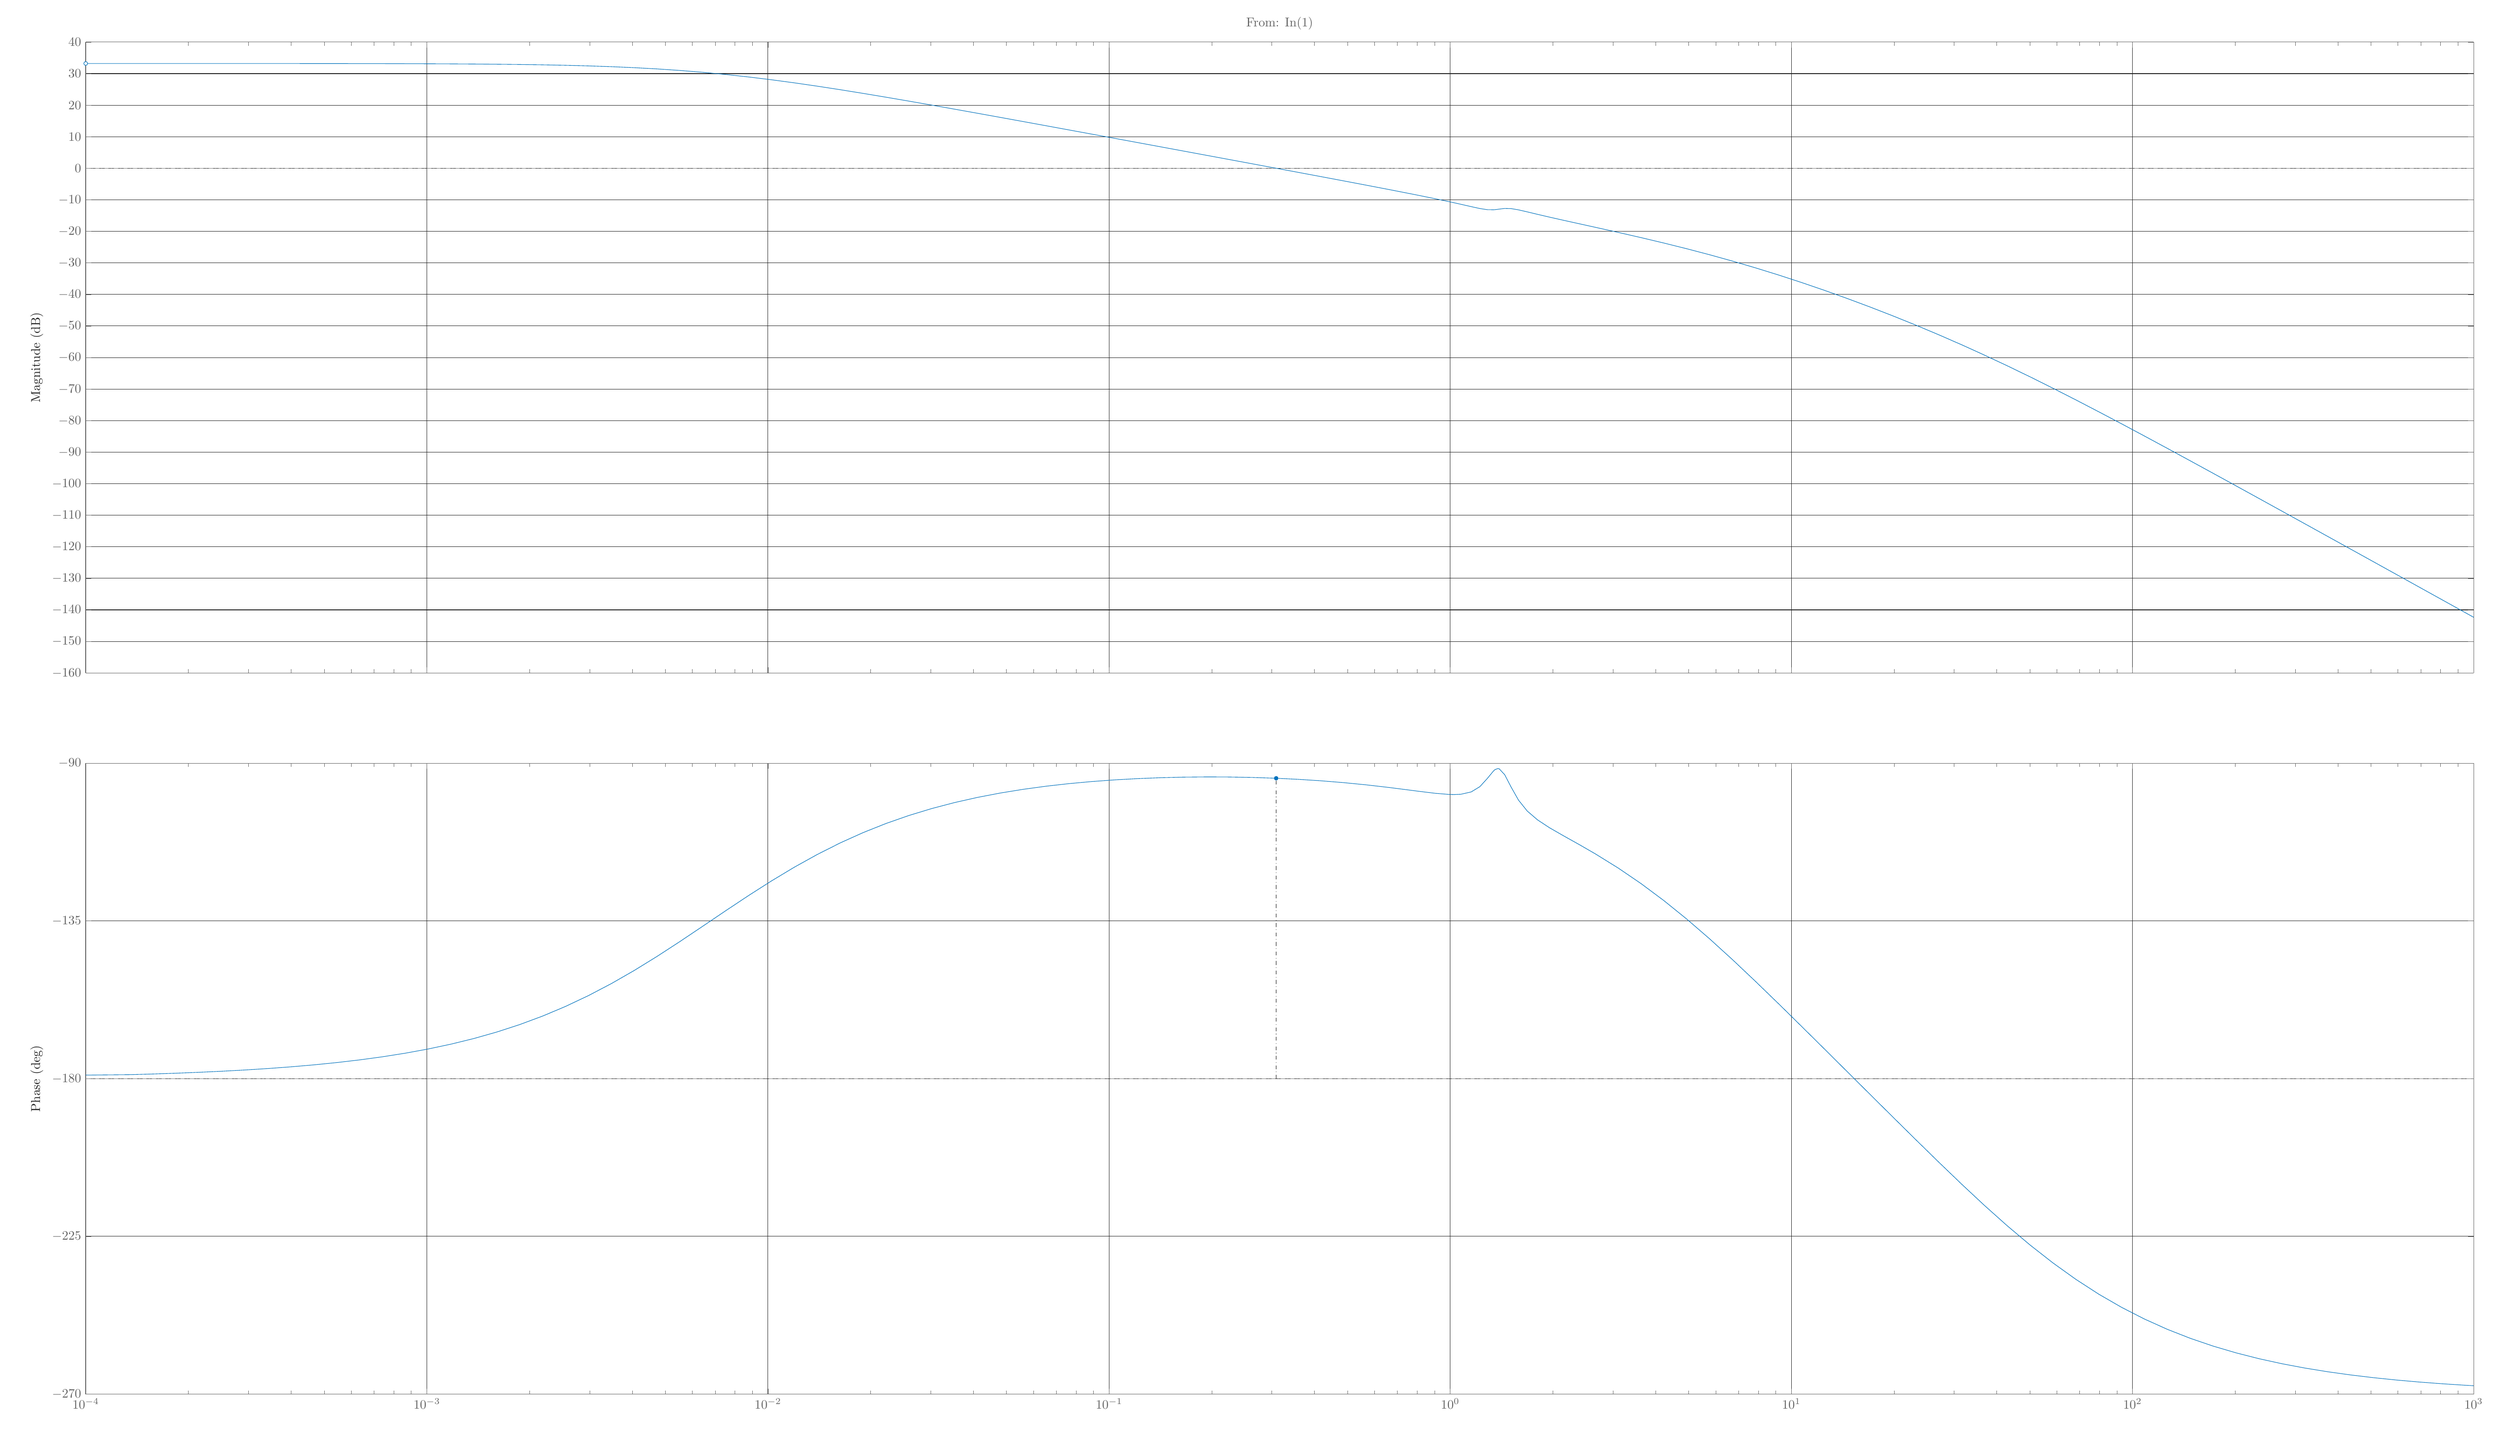
\begin{tikzpicture}

\begin{axis}[%
width=25.775in,
height=6.812in,
at={(0.787in,0.309in)},
scale only axis,
unbounded coords=jump,
separate axis lines,
every outer x axis line/.append style={mycolor3},
every x tick label/.append style={font=\color{mycolor3}},
every x tick/.append style={mycolor3},
xmode=log,
xmin=0.0001,
xmax=1000,
xminorticks=true,
every outer y axis line/.append style={mycolor3},
every y tick label/.append style={font=\color{mycolor3}},
every y tick/.append style={mycolor3},
ymin=-270,
ymax=-90,
ytick={-270, -225, -180, -135,  -90},
ylabel style={font=\color{mycolor4}},
ylabel={Phase (deg)},
axis background/.style={fill=white},
xmajorgrids,
ymajorgrids,
grid style={mycolor4}
]
\addplot [color=mycolor1, line width=1.5pt, forget plot]
  table[row sep=crcr]{%
nan	-270\\
nan	-90\\
};
\addplot [color=mycolor1, line width=1.5pt, forget plot]
  table[row sep=crcr]{%
nan	-270\\
nan	-90\\
};
\addplot [color=mycolor1, dashdotted, forget plot]
  table[row sep=crcr]{%
0.0001	-180\\
1000	-180\\
nan	nan\\
0.0001	-360\\
1000	-360\\
nan	nan\\
};
\addplot [color=mycolor1, dashdotted, forget plot]
  table[row sep=crcr]{%
0.308868678965405	-180\\
0.308868678965405	-94.2942065034725\\
nan	nan\\
};
\addplot [color=mycolor2, forget plot]
  table[row sep=crcr]{%
-1e+20	-270\\
-1.75e+18	-270\\
-17500000000000	-269.999999999864\\
-1750000000	-269.99999863543\\
-1750000	-269.998635430402\\
-17500	-269.863543193999\\
-1750	-268.635584214787\\
-1499.51714660695	-268.407733967093\\
-1284.88667026756	-268.141861352417\\
-1100.97691057881	-267.831637562135\\
-943.390717389296	-267.469689865374\\
-808.360318100044	-267.04743501152\\
-692.657232930092	-266.554889352785\\
-593.515084285712	-265.980454435204\\
-508.563454660737	-265.310678100672\\
-435.771211657966	-264.529993480644\\
-373.397945073603	-263.620442239832\\
-319.95235494038	-262.561394916269\\
-274.156595617355	-261.329291418802\\
-234.915723419207	-259.897440266105\\
-201.291517299815	-258.235937785327\\
-172.480046661486	-256.311799716545\\
-147.792449952265	-254.089437301325\\
-126.638464481412	-251.531653327372\\
-108.512313662772	-248.601366879305\\
-92.9806142601818	-245.264269189292\\
-79.6720145058224	-241.492517310478\\
-68.2683153463989	-237.269324799649\\
-58.4968625325115	-232.593869899189\\
-50.1240276515489	-227.485372563125\\
-42.9496222402847	-221.984740260228\\
-36.8021114226273	-216.152272499143\\
-31.5345126340395	-210.060896142796\\
-27.0208813740775	-203.786128190837\\
-23.1532999639208	-197.395596005958\\
-19.8392973122476	-190.941453821351\\
-16.9996379979133	-184.458046044911\\
-14.5664278079897	-177.965285103381\\
-12.4814904359387	-171.47641791628\\
-10.6949765279433	-165.007735847905\\
-9.16417182069131	-158.587370542645\\
-7.85247587404504	-152.260496177329\\
-6.72852698082737	-146.089088678084\\
-5.76545233094749	-140.145948962113\\
-4.940225501829	-134.504609951333\\
-4.23311591319856	-129.228075035594\\
-3.62721708309484	-124.359117605372\\
-3.10804240603791	-119.912715904844\\
-2.66317878870592	-115.866481575213\\
-2.39237635077625	-113.251005292419\\
-2.14399148550879	-110.661458933364\\
-1.95196026166226	-108.377130614364\\
-1.80130128659818	-106.140061807877\\
-1.68160667044661	-103.639294238503\\
-1.58548448116874	-100.534832319269\\
-1.50757886072228	-96.769102124804\\
-1.44393831174424	-93.2646549712019\\
-1.39159923312489	-91.5922210080171\\
-1.37957330551108	-91.5262736881954\\
-1.35500109262074	-91.7876340630653\\
-1.34115731252706	-92.1379646571659\\
-1.28454204027906	-94.3523862545132\\
-1.22142376581715	-96.6903547713756\\
-1.15160605608174	-98.199375732972\\
-1.07508301917166	-98.8555795953017\\
-1.02608589786395	-98.9451321714001\\
-0.992104431462472	-98.9109068480215\\
-0.903244457229836	-98.5837193879302\\
-0.809466464172925	-98.0197445405566\\
-0.773940231521988	-97.772508766217\\
-0.663163798637812	-96.9370357451874\\
-0.568243135466512	-96.1848533999579\\
-0.486908757184988	-95.5427539908611\\
-0.41721601727541	-95.0140809352767\\
-0.357498612424878	-94.5949793561642\\
-0.306328742411026	-94.279907448024\\
-0.262482972425072	-94.0637455219419\\
-0.224912981625002	-93.9426712194601\\
-0.19863774351497	-93.9127762453995\\
-0.192720498537819	-93.9145479687951\\
-0.165135824034342	-93.9791161613386\\
-0.141499428376322	-94.1381097565459\\
-0.121246182334501	-94.3953536061834\\
-0.103891845354981	-94.7568666364944\\
-0.0890214877156746	-95.2309805869888\\
-0.0762795698549222	-95.8284740612735\\
-0.0653614416761475	-96.5627127684196\\
-0.0560060585830474	-97.4497762934137\\
-0.0479897400909444	-98.5085373052574\\
-0.0411208217871896	-99.7606386653783\\
-0.0352350727728339	-101.230285578062\\
-0.0301917690198903	-102.943733059283\\
-0.025870328760984	-104.928306282853\\
-0.0221674294659739	-107.210752889781\\
-0.0189945374745302	-109.814715652381\\
-0.0162757912199579	-112.757173889708\\
-0.0139461874336695	-116.043893582795\\
-0.011950026963761	-119.664304162012\\
-0.0102395830483285	-123.586770743469\\
-0.00877396020289968	-127.755780118618\\
-0.00751811643879716	-132.09273240116\\
-0.00644202543437937	-136.501408360573\\
-0.00551995862727425	-140.877694026049\\
-0.00472987006294781	-145.121396576552\\
-0.00405286929177892	-149.147024682974\\
-0.00347276971198814	-152.890890490407\\
-0.00297570155962485	-156.313481847266\\
-0.00254978029248142	-159.397736860946\\
-0.00218482243923221	-162.144801361418\\
-0.00187210211995446	-164.568914922956\\
-0.00160414241661196	-166.692602269357\\
-0.00137453660531951	-168.542766100343\\
-0.00117779497618029	-170.147831159595\\
-0.00100921357826849	-171.535837120674\\
-0.000864761751544091	-172.733279347296\\
-0.000740985756668696	-173.764488576256\\
-0.000634926198580705	-174.651372951444\\
-0.000544047269486705	-175.413388796747\\
-0.000466176119520002	-176.067645991237\\
-0.000399450905462247	-176.629085041501\\
-0.000342276275410463	-177.110685670602\\
-0.000293285225059857	-177.523682399367\\
-0.000251306413613562	-177.877772959642\\
-0.00021533615786619	-178.181312017367\\
-0.000184514434859893	-178.441486803702\\
-0.000158104319353657	-178.664473721542\\
-0.000135474364470531	-178.855576406934\\
-1.35474364470531e-05	-179.885542518273\\
-1.35474364470531e-07	-179.998855423655\\
-1.35474364470531e-10	-179.999998855424\\
-1.35474364470531e-14	-179.999999999885\\
-1.35474364470531e-19	-180\\
-1e-20	-180\\
1e-20	-180\\
1.35474364470531e-19	-180\\
1.35474364470531e-14	-179.999999999885\\
1.35474364470531e-10	-179.999998855424\\
1.35474364470531e-07	-179.998855423655\\
1.35474364470531e-05	-179.885542518273\\
0.000135474364470531	-178.855576406934\\
0.000158104319353657	-178.664473721542\\
0.000184514434859893	-178.441486803702\\
0.00021533615786619	-178.181312017367\\
0.000251306413613562	-177.877772959642\\
0.000293285225059857	-177.523682399367\\
0.000342276275410463	-177.110685670602\\
0.000399450905462247	-176.629085041501\\
0.000466176119520002	-176.067645991237\\
0.000544047269486705	-175.413388796747\\
0.000634926198580705	-174.651372951444\\
0.000740985756668696	-173.764488576256\\
0.000864761751544091	-172.733279347296\\
0.00100921357826849	-171.535837120674\\
0.00117779497618029	-170.147831159595\\
0.00137453660531951	-168.542766100343\\
0.00160414241661196	-166.692602269357\\
0.00187210211995446	-164.568914922956\\
0.00218482243923221	-162.144801361418\\
0.00254978029248142	-159.397736860946\\
0.00297570155962485	-156.313481847266\\
0.00347276971198814	-152.890890490407\\
0.00405286929177892	-149.147024682974\\
0.00472987006294781	-145.121396576552\\
0.00551995862727425	-140.877694026049\\
0.00644202543437937	-136.501408360573\\
0.00751811643879716	-132.09273240116\\
0.00877396020289968	-127.755780118618\\
0.0102395830483285	-123.586770743469\\
0.011950026963761	-119.664304162012\\
0.0139461874336695	-116.043893582795\\
0.0162757912199579	-112.757173889708\\
0.0189945374745302	-109.814715652381\\
0.0221674294659739	-107.210752889781\\
0.025870328760984	-104.928306282853\\
0.0301917690198903	-102.943733059283\\
0.0352350727728339	-101.230285578062\\
0.0411208217871896	-99.7606386653783\\
0.0479897400909444	-98.5085373052574\\
0.0560060585830474	-97.4497762934137\\
0.0653614416761475	-96.5627127684196\\
0.0762795698549222	-95.8284740612735\\
0.0890214877156746	-95.2309805869888\\
0.103891845354981	-94.7568666364944\\
0.121246182334501	-94.3953536061834\\
0.141499428376322	-94.1381097565459\\
0.165135824034342	-93.9791161613386\\
0.192720498537819	-93.9145479687951\\
0.19863774351497	-93.9127762453995\\
0.224912981625002	-93.9426712194601\\
0.262482972425072	-94.0637455219419\\
0.306328742411026	-94.279907448024\\
0.357498612424878	-94.5949793561642\\
0.41721601727541	-95.0140809352767\\
0.486908757184988	-95.5427539908611\\
0.568243135466512	-96.1848533999579\\
0.663163798637812	-96.9370357451874\\
0.773940231521988	-97.772508766217\\
0.809466464172925	-98.0197445405566\\
0.903244457229836	-98.5837193879302\\
0.992104431462472	-98.9109068480215\\
1.02608589786395	-98.9451321714001\\
1.07508301917166	-98.8555795953017\\
1.15160605608174	-98.199375732972\\
1.22142376581715	-96.6903547713756\\
1.28454204027906	-94.3523862545132\\
1.34115731252706	-92.1379646571659\\
1.35500109262074	-91.7876340630653\\
1.37957330551108	-91.5262736881954\\
1.39159923312489	-91.5922210080171\\
1.44393831174424	-93.2646549712019\\
1.50757886072228	-96.769102124804\\
1.58548448116874	-100.534832319269\\
1.68160667044661	-103.639294238503\\
1.80130128659818	-106.140061807877\\
1.95196026166226	-108.377130614364\\
2.14399148550879	-110.661458933364\\
2.39237635077625	-113.251005292419\\
2.66317878870592	-115.866481575213\\
3.10804240603791	-119.912715904844\\
3.62721708309484	-124.359117605372\\
4.23311591319856	-129.228075035594\\
4.940225501829	-134.504609951333\\
5.76545233094749	-140.145948962113\\
6.72852698082737	-146.089088678084\\
7.85247587404504	-152.260496177329\\
9.16417182069131	-158.587370542645\\
10.6949765279433	-165.007735847905\\
12.4814904359387	-171.47641791628\\
14.5664278079897	-177.965285103381\\
16.9996379979133	-184.458046044911\\
19.8392973122476	-190.941453821351\\
23.1532999639208	-197.395596005958\\
27.0208813740775	-203.786128190837\\
31.5345126340395	-210.060896142796\\
36.8021114226273	-216.152272499143\\
42.9496222402847	-221.984740260228\\
50.1240276515489	-227.485372563125\\
58.4968625325115	-232.593869899189\\
68.2683153463989	-237.269324799649\\
79.6720145058224	-241.492517310478\\
92.9806142601818	-245.264269189292\\
108.512313662772	-248.601366879305\\
126.638464481412	-251.531653327372\\
147.792449952265	-254.089437301325\\
172.480046661486	-256.311799716545\\
201.291517299815	-258.235937785327\\
234.915723419207	-259.897440266105\\
274.156595617355	-261.329291418802\\
319.95235494038	-262.561394916269\\
373.397945073603	-263.620442239832\\
435.771211657966	-264.529993480644\\
508.563454660737	-265.310678100672\\
593.515084285712	-265.980454435204\\
692.657232930092	-266.554889352785\\
808.360318100044	-267.04743501152\\
943.390717389296	-267.469689865374\\
1100.97691057881	-267.831637562135\\
1284.88667026756	-268.141861352417\\
1499.51714660695	-268.407733967093\\
1750	-268.635584214787\\
17500	-269.863543193999\\
1750000	-269.998635430402\\
1750000000	-269.99999863543\\
17500000000000	-269.999999999864\\
1.75e+18	-270\\
1e+20	-270\\
};
\addplot[only marks, mark=*, mark options={}, mark size=1.5000pt, draw=mycolor2, fill=white, forget plot] table[row sep=crcr]{%
x	y\\
nan	nan\\
};
\addplot[only marks, mark=*, mark options={}, mark size=1.5000pt, draw=mycolor2, fill=mycolor2, forget plot] table[row sep=crcr]{%
x	y\\
0.308868678965405	-94.296749653314\\
};
\end{axis}

\begin{axis}[%
width=25.775in,
height=6.812in,
at={(0.787in,8.095in)},
scale only axis,
unbounded coords=jump,
separate axis lines,
every outer x axis line/.append style={mycolor3},
every x tick label/.append style={font=\color{mycolor3}},
every x tick/.append style={mycolor3},
xmode=log,
xmin=0.0001,
xmax=1000,
xtick={0.0001,0.001,0.01,0.1,1,10,100,1000},
xticklabels={\empty},
xminorticks=true,
every outer y axis line/.append style={mycolor3},
every y tick label/.append style={font=\color{mycolor3}},
every y tick/.append style={mycolor3},
ymin=-160,
ymax=40,
ylabel style={font=\color{mycolor4}},
ylabel={Magnitude (dB)},
axis background/.style={fill=white},
title style={font=\color{mycolor3}},
title={From: In(1)},
xmajorgrids,
ymajorgrids,
grid style={mycolor4}
]
\addplot [color=mycolor1, line width=1.5pt, forget plot]
  table[row sep=crcr]{%
nan	-160\\
nan	40\\
};
\addplot [color=mycolor1, line width=1.5pt, forget plot]
  table[row sep=crcr]{%
nan	-160\\
nan	40\\
};
\addplot [color=mycolor1, dashdotted, forget plot]
  table[row sep=crcr]{%
0.0001	0\\
1000	0\\
};
\addplot [color=mycolor1, dashdotted, forget plot]
  table[row sep=crcr]{%
0	0\\
0	33.2134315544518\\
nan	nan\\
};
\addplot [color=mycolor2, forget plot]
  table[row sep=crcr]{%
-1e+20	-1162.33530552371\\
-1.75e+18	-1056.91758844489\\
-17500000000000	-756.917588444891\\
-1750000000	-516.917588444891\\
-1750000	-336.917588446691\\
-17500	-216.917606446369\\
-1750	-156.919388248399\\
-1499.51714660695	-152.894842833186\\
-1284.88667026756	-148.870533047021\\
-1100.97691057881	-144.846544059612\\
-943.390717389296	-140.822991764238\\
-808.360318100044	-136.800033808226\\
-692.657232930092	-132.777884538844\\
-593.515084285712	-128.756835216276\\
-508.563454660737	-124.737281279408\\
-435.771211657966	-120.719758995443\\
-373.397945073603	-116.704994483939\\
-319.95235494038	-112.693968855146\\
-274.156595617355	-108.688003958723\\
-234.915723419207	-104.688873808669\\
-201.291517299815	-100.698946744807\\
-172.480046661486	-96.7213621040513\\
-147.792449952265	-92.7602414391038\\
-126.638464481412	-88.8209264236759\\
-108.512313662772	-84.9102214387509\\
-92.9806142601818	-81.0365968607913\\
-79.6720145058224	-77.2102803618677\\
-68.2683153463989	-73.4431356670038\\
-58.4968625325115	-69.7482194076853\\
-50.1240276515489	-66.1389451850359\\
-42.9496222402847	-62.6278939587986\\
-36.8021114226273	-59.2254809744773\\
-31.5345126340395	-55.9388486013993\\
-27.0208813740775	-52.7713852758664\\
-23.1532999639208	-49.7231002717167\\
-19.8392973122476	-46.7917702654108\\
-16.9996379979133	-43.9744838069135\\
-14.5664278079897	-41.269088342187\\
-12.4814904359387	-38.675110909407\\
-10.6949765279433	-36.1939006123003\\
-9.16417182069131	-33.8279508620485\\
-7.85247587404504	-31.5795712121497\\
-6.72852698082737	-29.4492724528002\\
-5.76545233094749	-27.4343427216389\\
-4.940225501829	-25.5280357973372\\
-4.23311591319856	-23.7195325163206\\
-3.62721708309484	-21.9944587942421\\
-3.10804240603791	-20.3353782169575\\
-2.66317878870592	-18.7212931229198\\
-2.39237635077625	-17.613064012835\\
-2.14399148550879	-16.4751451020785\\
-1.95196026166226	-15.4811376469751\\
-1.80130128659818	-14.6016814614468\\
-1.68160667044661	-13.8271722742804\\
-1.58548448116874	-13.1897891659639\\
-1.50757886072228	-12.7917033992952\\
-1.44393831174424	-12.7445777084054\\
-1.39159923312489	-12.9533927404257\\
-1.37957330551108	-13.0144073694213\\
-1.35500109262074	-13.1237322599761\\
-1.34115731252706	-13.1666990111837\\
-1.28454204027906	-13.136708798086\\
-1.22142376581715	-12.7674170245774\\
-1.15160605608174	-12.1635770979372\\
-1.07508301917166	-11.4261318795501\\
-1.02608589786395	-10.9373181368381\\
-0.992104431462472	-10.5921200383121\\
-0.903244457229836	-9.66012224951349\\
-0.809466464172925	-8.61232073021029\\
-0.773940231521988	-8.19224328772885\\
-0.663163798637812	-6.77277288193553\\
-0.568243135466512	-5.38038810214674\\
-0.486908757184988	-4.00446209030324\\
-0.41721601727541	-2.63914312248487\\
-0.357498612424878	-1.28096350948891\\
-0.306328742411026	0.0722415020065339\\
-0.262482972425072	1.42186678654927\\
-0.224912981625002	2.76882030286144\\
-0.19863774351497	3.8505373313111\\
-0.192720498537819	4.11368148535265\\
-0.165135824034342	5.45679204550537\\
-0.141499428376322	6.79830665140643\\
-0.121246182334501	8.13821718146317\\
-0.103891845354981	9.47635725313969\\
-0.0890214877156746	10.8123898072428\\
-0.0762795698549222	12.1457780566809\\
-0.0653614416761475	13.4757383474418\\
-0.0560060585830474	14.8011721215145\\
-0.0479897400909444	16.1205731794969\\
-0.0411208217871896	17.4319060286855\\
-0.0352350727728339	18.7324518021375\\
-0.0301917690198903	20.0186210141922\\
-0.025870328760984	21.2857387951801\\
-0.0221674294659739	22.5278202318032\\
-0.0189945374745302	23.7373729631507\\
-0.0162757912199579	24.9052914506339\\
-0.0139461874336695	26.0209375551542\\
-0.011950026963761	27.0725210299357\\
-0.0102395830483285	28.0478757532044\\
-0.00877396020289968	28.935644411693\\
-0.00751811643879716	29.7267297278124\\
-0.00644202543437937	30.4156933940213\\
-0.00551995862727425	31.0016915232541\\
-0.00472987006294781	31.4886265080871\\
-0.00405286929177892	31.8844603065633\\
-0.00347276971198814	32.1999312636264\\
-0.00297570155962485	32.4470772922834\\
-0.00254978029248142	32.6379324681316\\
-0.00218482243923221	32.7836029149014\\
-0.00187210211995446	32.8937563486602\\
-0.00160414241661196	32.9764500016297\\
-0.00137453660531951	33.0381838252975\\
-0.00117779497618029	33.0840753849855\\
-0.00100921357826849	33.1180813694946\\
-0.000864761751544091	33.1432198970086\\
-0.000740985756668696	33.1617702130551\\
-0.000634926198580705	33.1754408665694\\
-0.000544047269486705	33.1855056143245\\
-0.000466176119520002	33.1929102411686\\
-0.000399450905462247	33.1983549221354\\
-0.000342276275410463	33.2023568711692\\
-0.000293285225059857	33.2052975355676\\
-0.000251306413613562	33.2074579013614\\
-0.00021533615786619	33.2090447716537\\
-0.000184514434859893	33.21021025433\\
-0.000158104319353657	33.2110661753019\\
-0.000135474364470531	33.2116947178264\\
-1.35474364470531e-05	33.2134141826469\\
-1.35474364470531e-07	33.2134315527146\\
-1.35474364470531e-10	33.2134315544518\\
-1.35474364470531e-14	33.2134315544518\\
-1.35474364470531e-19	33.2134315544518\\
-1e-20	33.2134315544518\\
1e-20	33.2134315544518\\
1.35474364470531e-19	33.2134315544518\\
1.35474364470531e-14	33.2134315544518\\
1.35474364470531e-10	33.2134315544518\\
1.35474364470531e-07	33.2134315527146\\
1.35474364470531e-05	33.2134141826469\\
0.000135474364470531	33.2116947178264\\
0.000158104319353657	33.2110661753019\\
0.000184514434859893	33.21021025433\\
0.00021533615786619	33.2090447716537\\
0.000251306413613562	33.2074579013614\\
0.000293285225059857	33.2052975355676\\
0.000342276275410463	33.2023568711692\\
0.000399450905462247	33.1983549221354\\
0.000466176119520002	33.1929102411686\\
0.000544047269486705	33.1855056143245\\
0.000634926198580705	33.1754408665694\\
0.000740985756668696	33.1617702130551\\
0.000864761751544091	33.1432198970086\\
0.00100921357826849	33.1180813694946\\
0.00117779497618029	33.0840753849855\\
0.00137453660531951	33.0381838252975\\
0.00160414241661196	32.9764500016297\\
0.00187210211995446	32.8937563486602\\
0.00218482243923221	32.7836029149014\\
0.00254978029248142	32.6379324681316\\
0.00297570155962485	32.4470772922834\\
0.00347276971198814	32.1999312636264\\
0.00405286929177892	31.8844603065633\\
0.00472987006294781	31.4886265080871\\
0.00551995862727425	31.0016915232541\\
0.00644202543437937	30.4156933940213\\
0.00751811643879716	29.7267297278124\\
0.00877396020289968	28.935644411693\\
0.0102395830483285	28.0478757532044\\
0.011950026963761	27.0725210299357\\
0.0139461874336695	26.0209375551542\\
0.0162757912199579	24.9052914506339\\
0.0189945374745302	23.7373729631507\\
0.0221674294659739	22.5278202318032\\
0.025870328760984	21.2857387951801\\
0.0301917690198903	20.0186210141922\\
0.0352350727728339	18.7324518021375\\
0.0411208217871896	17.4319060286855\\
0.0479897400909444	16.1205731794969\\
0.0560060585830474	14.8011721215145\\
0.0653614416761475	13.4757383474418\\
0.0762795698549222	12.1457780566809\\
0.0890214877156746	10.8123898072428\\
0.103891845354981	9.47635725313969\\
0.121246182334501	8.13821718146317\\
0.141499428376322	6.79830665140643\\
0.165135824034342	5.45679204550537\\
0.192720498537819	4.11368148535265\\
0.19863774351497	3.8505373313111\\
0.224912981625002	2.76882030286144\\
0.262482972425072	1.42186678654927\\
0.306328742411026	0.0722415020065339\\
0.357498612424878	-1.28096350948891\\
0.41721601727541	-2.63914312248487\\
0.486908757184988	-4.00446209030324\\
0.568243135466512	-5.38038810214674\\
0.663163798637812	-6.77277288193553\\
0.773940231521988	-8.19224328772885\\
0.809466464172925	-8.61232073021029\\
0.903244457229836	-9.66012224951349\\
0.992104431462472	-10.5921200383121\\
1.02608589786395	-10.9373181368381\\
1.07508301917166	-11.4261318795501\\
1.15160605608174	-12.1635770979372\\
1.22142376581715	-12.7674170245774\\
1.28454204027906	-13.136708798086\\
1.34115731252706	-13.1666990111837\\
1.35500109262074	-13.1237322599761\\
1.37957330551108	-13.0144073694213\\
1.39159923312489	-12.9533927404257\\
1.44393831174424	-12.7445777084054\\
1.50757886072228	-12.7917033992952\\
1.58548448116874	-13.1897891659639\\
1.68160667044661	-13.8271722742804\\
1.80130128659818	-14.6016814614468\\
1.95196026166226	-15.4811376469751\\
2.14399148550879	-16.4751451020785\\
2.39237635077625	-17.613064012835\\
2.66317878870592	-18.7212931229198\\
3.10804240603791	-20.3353782169575\\
3.62721708309484	-21.9944587942421\\
4.23311591319856	-23.7195325163206\\
4.940225501829	-25.5280357973372\\
5.76545233094749	-27.4343427216389\\
6.72852698082737	-29.4492724528002\\
7.85247587404504	-31.5795712121497\\
9.16417182069131	-33.8279508620485\\
10.6949765279433	-36.1939006123003\\
12.4814904359387	-38.675110909407\\
14.5664278079897	-41.269088342187\\
16.9996379979133	-43.9744838069135\\
19.8392973122476	-46.7917702654108\\
23.1532999639208	-49.7231002717167\\
27.0208813740775	-52.7713852758664\\
31.5345126340395	-55.9388486013993\\
36.8021114226273	-59.2254809744773\\
42.9496222402847	-62.6278939587986\\
50.1240276515489	-66.1389451850359\\
58.4968625325115	-69.7482194076853\\
68.2683153463989	-73.4431356670038\\
79.6720145058224	-77.2102803618677\\
92.9806142601818	-81.0365968607913\\
108.512313662772	-84.9102214387509\\
126.638464481412	-88.8209264236759\\
147.792449952265	-92.7602414391038\\
172.480046661486	-96.7213621040513\\
201.291517299815	-100.698946744807\\
234.915723419207	-104.688873808669\\
274.156595617355	-108.688003958723\\
319.95235494038	-112.693968855146\\
373.397945073603	-116.704994483939\\
435.771211657966	-120.719758995443\\
508.563454660737	-124.737281279408\\
593.515084285712	-128.756835216276\\
692.657232930092	-132.777884538844\\
808.360318100044	-136.800033808226\\
943.390717389296	-140.822991764238\\
1100.97691057881	-144.846544059612\\
1284.88667026756	-148.870533047021\\
1499.51714660695	-152.894842833186\\
1750	-156.919388248399\\
17500	-216.917606446369\\
1750000	-336.917588446691\\
1750000000	-516.917588444891\\
17500000000000	-756.917588444891\\
1.75e+18	-1056.91758844489\\
1e+20	-1162.33530552371\\
};
\addplot[only marks, mark=*, mark options={}, mark size=1.5000pt, draw=mycolor2, fill=white, forget plot] table[row sep=crcr]{%
x	y\\
0.0001	33.2119214415097\\
};
\addplot[only marks, mark=*, mark options={}, mark size=1.5000pt, draw=mycolor2, fill=mycolor2, forget plot] table[row sep=crcr]{%
x	y\\
0	33.2134315544518\\
};
\end{axis}

\begin{axis}[%
width=26.667in,
height=15in,
at={(0in,0in)},
scale only axis,
xmin=0,
xmax=1,
ymin=0,
ymax=1,
axis line style={draw=none},
ticks=none,
axis x line*=bottom,
axis y line*=left
]
\end{axis}
\end{tikzpicture}%
\caption{Design A analysis: (left) Root locus with closed-loop poles marked in red; (right) Open-loop Bode plot showing PM = 42°.}
\label{fig:design_A_rlocus}
\label{fig:design_A_bode}
\end{figure}

\begin{figure}[h!]
\centering
\resizebox{0.7\textwidth}{!}{% This file was created by matlab2tikz.
%
\definecolor{mycolor1}{rgb}{0.49020,0.49020,0.49020}%
\definecolor{mycolor2}{rgb}{0.00000,0.44700,0.74100}%
\definecolor{mycolor3}{rgb}{0.38039,0.38039,0.38039}%
\definecolor{mycolor4}{rgb}{0.12941,0.12941,0.12941}%
%
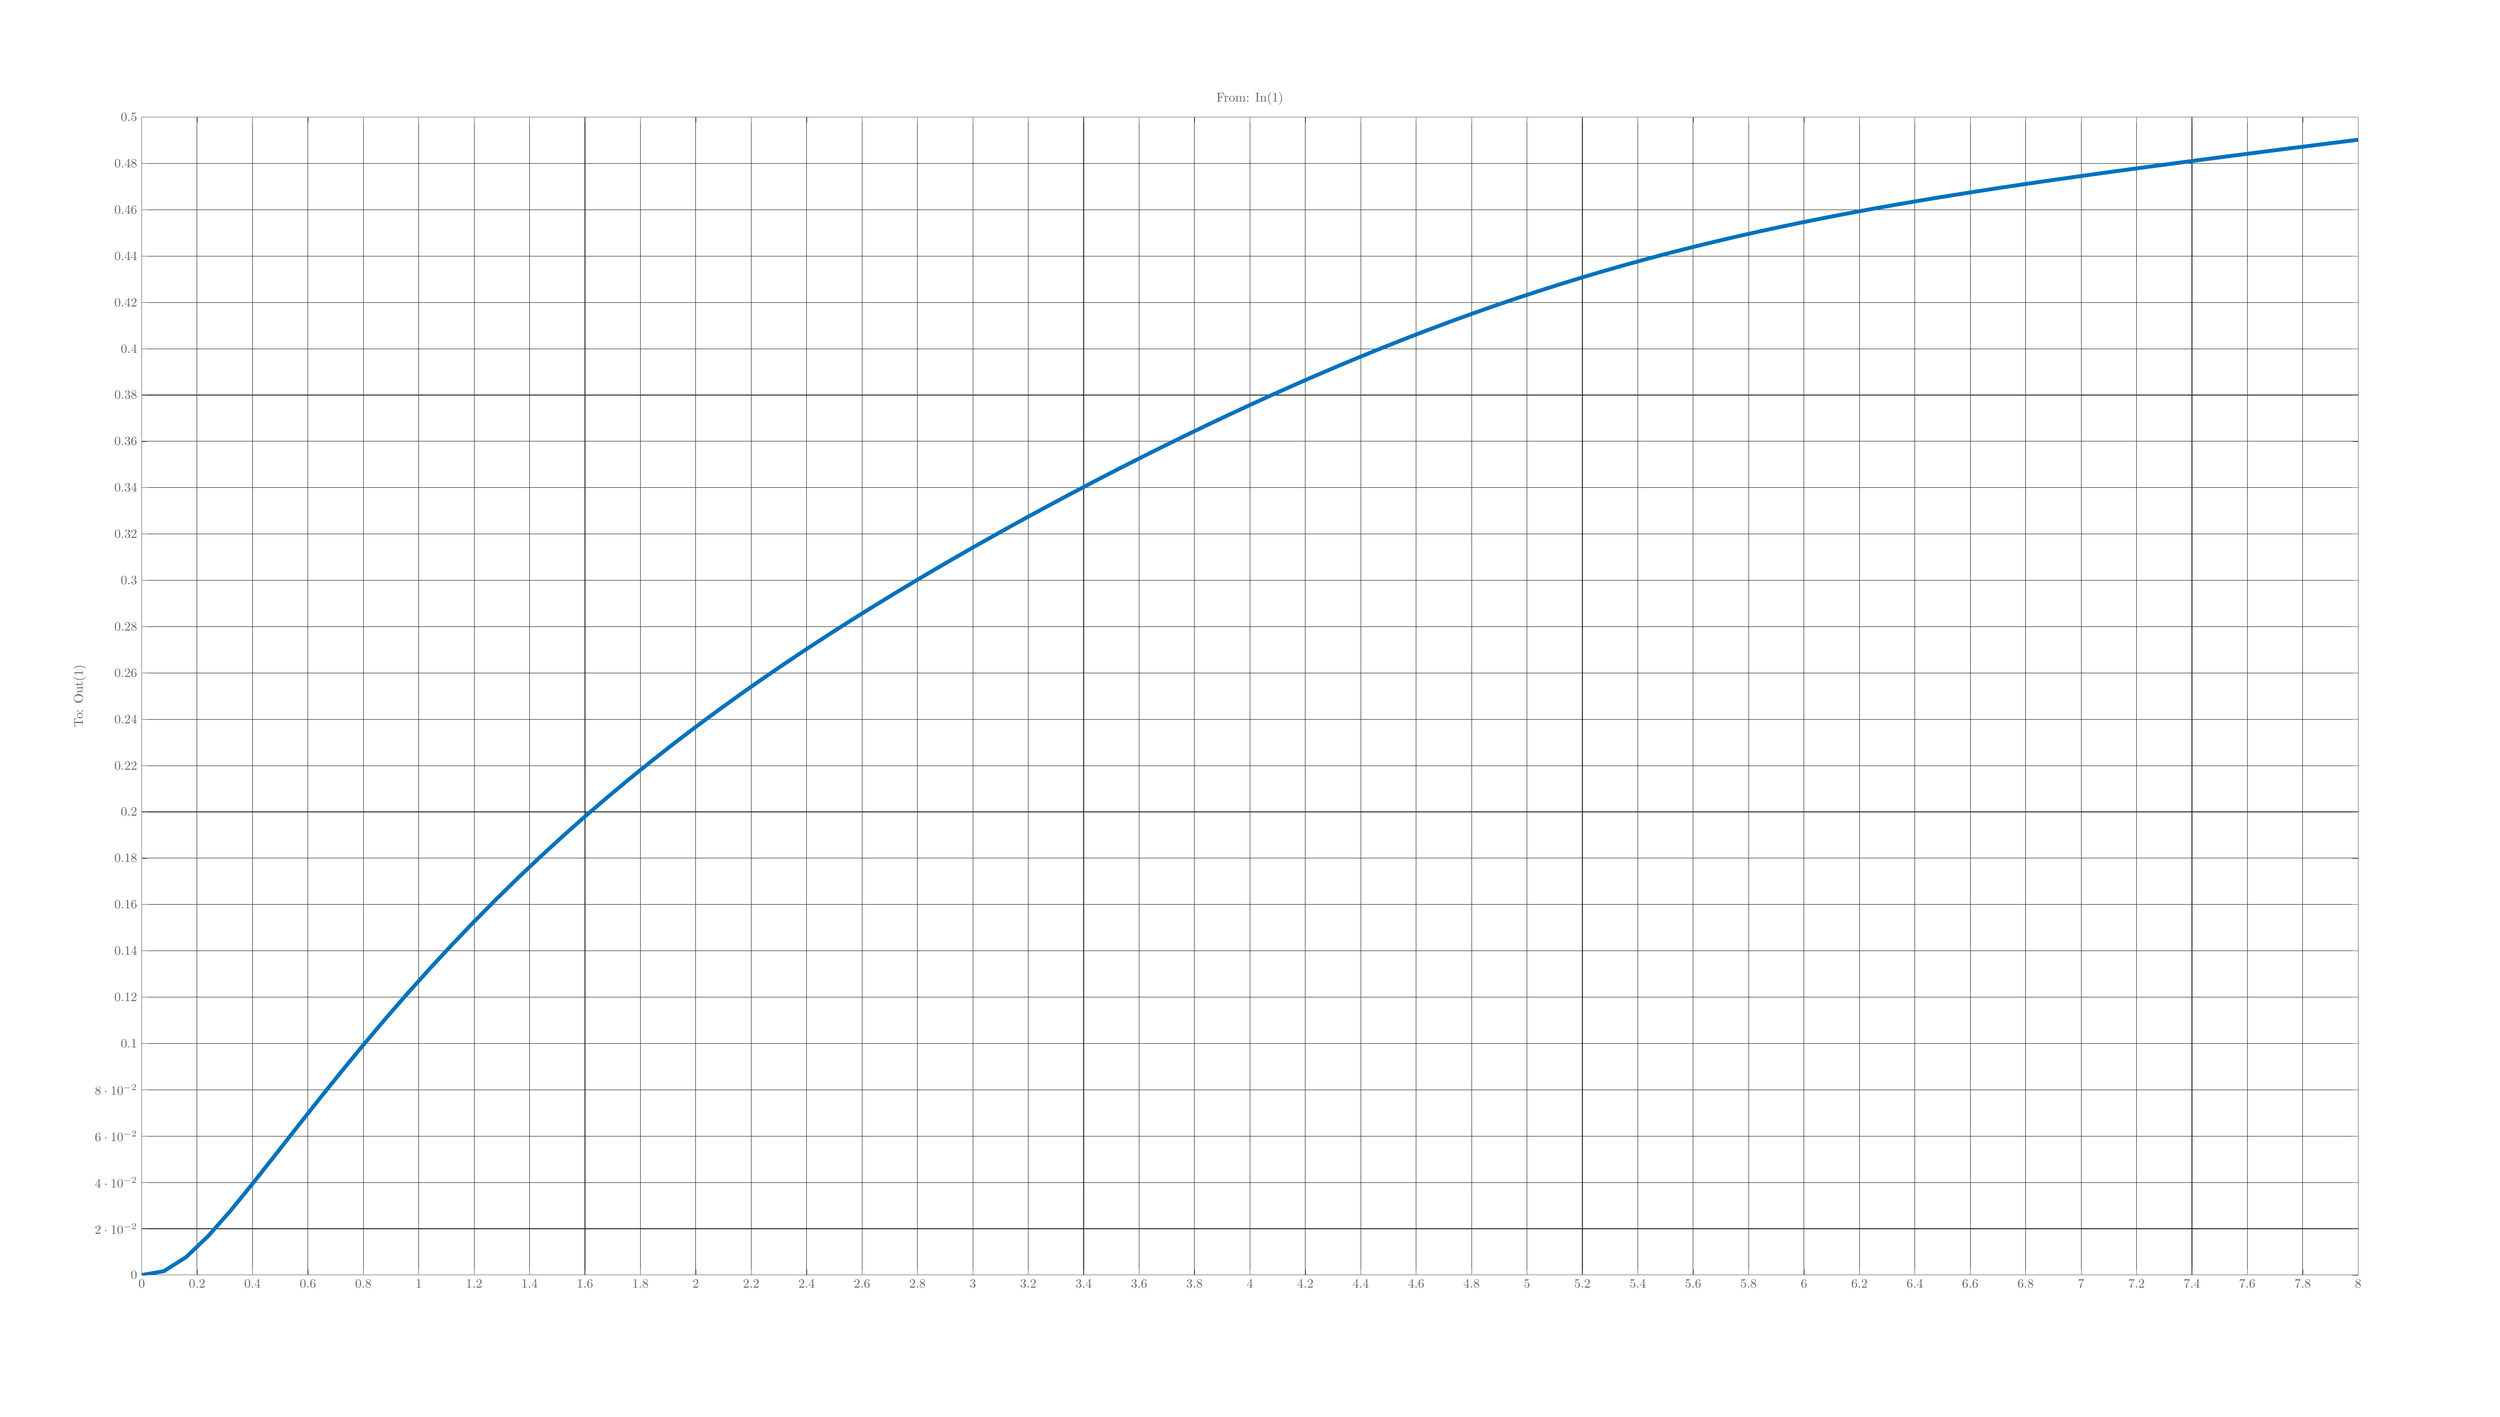
\begin{tikzpicture}

\begin{axis}[%
width=23.889in,
height=12.486in,
at={(1.389in,1.389in)},
scale only axis,
separate axis lines,
every outer x axis line/.append style={mycolor3},
every x tick label/.append style={font=\color{mycolor3}},
every x tick/.append style={mycolor3},
xmin=0,
xmax=8,
every outer y axis line/.append style={mycolor3},
every y tick label/.append style={font=\color{mycolor3}},
every y tick/.append style={mycolor3},
ymin=0,
ymax=0.5,
ylabel style={font=\color{mycolor3}},
ylabel={To: Out(1)},
axis background/.style={fill=white},
title style={font=\color{mycolor3}},
title={From: In(1)},
xmajorgrids,
ymajorgrids,
grid style={mycolor4}
]
\addplot [color=mycolor1, dotted, forget plot]
  table[row sep=crcr]{%
0	0.535291584116315\\
8	0.535291584116315\\
};
\addplot [color=mycolor2, line width=3.0pt, forget plot]
  table[row sep=crcr]{%
0	0\\
0.08	0.00166633828000285\\
0.16	0.00772776129654752\\
0.24	0.0168444615185643\\
0.32	0.0276891050097778\\
0.4	0.0394269714927952\\
0.48	0.0515516153659193\\
0.56	0.0637577153340131\\
0.64	0.0758623290357947\\
0.72	0.0877570527554796\\
0.8	0.099379007704982\\
0.88	0.110693241256829\\
0.96	0.121682044447503\\
1.04	0.132338458245484\\
1.12	0.142662315272741\\
1.2	0.15265781500003\\
1.28	0.162332025367422\\
1.36	0.171693943252564\\
1.44	0.180753891419733\\
1.52	0.189523117637576\\
1.6	0.198013515048617\\
1.68	0.206237415248289\\
1.76	0.214207425154976\\
1.84	0.221936290639169\\
1.92	0.229436777069563\\
2	0.236721561270372\\
2.08	0.24380313198549\\
2.16	0.250693697489864\\
2.24	0.25740509988837\\
2.32	0.263948736147999\\
2.4	0.270335486172439\\
2.48	0.276575648342411\\
2.56	0.282678882967151\\
2.64	0.288654164057621\\
2.72	0.29450973976228\\
2.8	0.300253101715502\\
2.88	0.305890963446102\\
2.96	0.311429247884927\\
3.04	0.316873083900376\\
3.12	0.322226811682057\\
3.2	0.327493996687922\\
3.28	0.332677451770881\\
3.36	0.337779267008699\\
3.44	0.342800846676907\\
3.52	0.347742952729659\\
3.6	0.352605754088587\\
3.68	0.357388880985395\\
3.76	0.362091483560597\\
3.84	0.36671229388868\\
3.92	0.371249690579197\\
4	0.375701765093823\\
4.08	0.380066388921008\\
4.16	0.384341280762232\\
4.24	0.388524072906593\\
4.32	0.392612376002906\\
4.4	0.396603841479988\\
4.48	0.400496220915675\\
4.56	0.404287421712306\\
4.64	0.407975558500236\\
4.72	0.411558999760212\\
4.8	0.415036409229222\\
4.88	0.418406781731734\\
4.96	0.421669473157793\\
5.04	0.424824224390456\\
5.12	0.427871179066173\\
5.2	0.430810895132199\\
5.28	0.43364435024373\\
5.36	0.436372941119441\\
5.44	0.438998477046445\\
5.52	0.441523167793654\\
5.6	0.443949606255363\\
5.68	0.446280746203917\\
5.76	0.448519875581016\\
5.84	0.450670585801137\\
5.92	0.452736737577269\\
6	0.454722423808464\\
6.08	0.456631930090421\\
6.16	0.458469693424358\\
6.24	0.460240259705861\\
6.32	0.461948240574349\\
6.4	0.463598270195414\\
6.48	0.465194962533041\\
6.56	0.466742869646801\\
6.64	0.468246441521104\\
6.72	0.469709987900013\\
6.8	0.471137642562468\\
6.88	0.472533330429761\\
6.96	0.473900737850333\\
7.04	0.475243286357164\\
7.12	0.476564110140911\\
7.2	0.477866037428172\\
7.28	0.479151575899658\\
7.36	0.480422902228232\\
7.44	0.481681855762476\\
7.52	0.482929936328352\\
7.6	0.484168306070251\\
7.68	0.485397795203825\\
7.76	0.486618911507146\\
7.84	0.487831853334253\\
7.92	0.489036525896632\\
8	0.490232560523908\\
};
\end{axis}

\begin{axis}[%
width=26.667in,
height=15in,
at={(0in,0in)},
scale only axis,
xmin=0,
xmax=1,
ymin=0,
ymax=1,
axis line style={draw=none},
ticks=none,
axis x line*=bottom,
axis y line*=left
]
\end{axis}
\end{tikzpicture}%}
\caption{Design A: Closed-loop step response for 30° bank command showing 22\% overshoot and 3.8~s settling time.}
\label{fig:design_A_step}
\end{figure}

\textbf{Performance Summary (Design A):}
\begin{center}
\begin{tabular}{lccc}
\hline
\textbf{Metric} & \textbf{Specification} & \textbf{Achieved} & \textbf{Pass/Fail} \\
\hline
$\omega_c$ & $[2,10]$~rad/s & 3.2~rad/s & \textcolor{green!60!black}{Pass} \\
Phase Margin & $>45^\circ$ (typical) & $42^\circ$ & \textcolor{red}{Marginal} \\
$T_s$ (2\%) & $\le 3$~s & 3.8~s & \textcolor{red}{Fail} \\
$M_p$ & $<20\%$ & 22\% & \textcolor{red}{Fail} \\
$e_{ss}$ & $<1\%$ & 3\% & \textcolor{red}{Fail} \\
$|\delta_a|_{\max}$ & $\le 20^\circ$ & 14.2$^\circ$ & \textcolor{green!60!black}{Pass} \\
\hline
\end{tabular}
\end{center}

\textbf{Conclusion:} P-only control provides fast response but suffers from excessive overshoot, slow settling, steady-state error, and marginal robustness. Integral action and phase lead are required.

\paragraph{Design Iteration B: Proportional-Integral (PI) Control}

Adding integral action eliminates steady-state error:
\begin{equation}
C_B(s) = K_p\left(1 + \frac{1}{T_i\,s}\right), \qquad K_p = -0.080,\; T_i = 0.60~\text{s}
\label{eq:design_B}
\end{equation}

\textbf{Analysis:}

\textbf{Root Locus:} Integral action adds a pole at origin, changing root locus topology. Dominant closed-loop poles at $s = -3.45 \pm 8.12j$ ($\zeta=0.39$, $\omega_n=8.82$~rad/s) show reduced damping (Figure~\ref{fig:design_B_rlocus}).

\textbf{Bode Plot:} Crossover frequency $\omega_c \approx 4.8$~rad/s with phase margin PM $\approx 38^\circ$. The integrator contributes $-90^\circ$ phase lag, degrading phase margin further (Figure~\ref{fig:design_B_bode}).

\textbf{Step Response:} Fast rise (0.38~s) but significant overshoot (28\%) and oscillatory settling (4.2~s). Zero steady-state error confirmed. Actuator briefly saturates at 19.8$^\circ$ (Figure~\ref{fig:design_B_step}).

\begin{figure}[h!]
\centering
\resizebox{0.48\textwidth}{!}{% This file was created by matlab2tikz.
%
\definecolor{mycolor1}{rgb}{0.85098,0.85098,0.85098}%
\definecolor{mycolor2}{rgb}{0.49020,0.49020,0.49020}%
\definecolor{mycolor3}{rgb}{0.92941,0.69412,0.12549}%
\definecolor{mycolor4}{rgb}{0.63529,0.07843,0.18431}%
\definecolor{mycolor5}{rgb}{0.30196,0.74510,0.93333}%
\definecolor{mycolor6}{rgb}{1.00000,0.27059,0.22745}%
\definecolor{mycolor7}{rgb}{0.46667,0.67451,0.18824}%
\definecolor{mycolor8}{rgb}{0.00000,0.44706,0.74118}%
\definecolor{mycolor9}{rgb}{0.85000,0.32500,0.09800}%
\definecolor{mycolor10}{rgb}{0.00000,0.44700,0.74100}%
\definecolor{mycolor11}{rgb}{0.92900,0.69400,0.12500}%
\definecolor{mycolor12}{rgb}{0.38039,0.38039,0.38039}%
%
\begin{tikzpicture}

\begin{axis}[%
width=23.889in,
height=12.486in,
at={(1.389in,1.389in)},
scale only axis,
unbounded coords=jump,
separate axis lines,
every outer x axis line/.append style={mycolor12},
every x tick label/.append style={font=\color{mycolor12}},
every x tick/.append style={mycolor12},
xmin=-120,
xmax=60,
every outer y axis line/.append style={mycolor12},
every y tick label/.append style={font=\color{mycolor12}},
every y tick/.append style={mycolor12},
ymin=-100,
ymax=100,
axis background/.style={fill=white},
legend style={legend cell align=left, align=left}
]
\addplot [color=mycolor1, dotted, forget plot]
  table[row sep=crcr]{%
0	0\\
-0	160\\
nan	nan\\
0	0\\
-25.6	157.938722294439\\
nan	nan\\
0	0\\
-48	152.630272226711\\
nan	nan\\
0	0\\
-73.6	142.067026434708\\
nan	nan\\
0	0\\
-96	128\\
nan	nan\\
0	0\\
-115.2	111.035850066544\\
nan	nan\\
0	0\\
-134.4	86.8138237840034\\
nan	nan\\
0	0\\
-147.2	62.7069374152494\\
nan	nan\\
0	0\\
-156.8	31.8395979874119\\
nan	nan\\
0	0\\
-160	0\\
nan	nan\\
0	-0\\
-0	-160\\
nan	nan\\
0	-0\\
-25.6	-157.938722294439\\
nan	nan\\
0	-0\\
-48	-152.630272226711\\
nan	nan\\
0	-0\\
-73.6	-142.067026434708\\
nan	nan\\
0	-0\\
-96	-128\\
nan	nan\\
0	-0\\
-115.2	-111.035850066544\\
nan	nan\\
0	-0\\
-134.4	-86.8138237840034\\
nan	nan\\
0	-0\\
-147.2	-62.7069374152494\\
nan	nan\\
0	-0\\
-156.8	-31.8395979874119\\
nan	nan\\
0	-0\\
-160	-0\\
nan	nan\\
};
\addplot [color=mycolor1, dotted, forget plot]
  table[row sep=crcr]{%
-0	0\\
-0	0\\
-0	0\\
-0	0\\
-0	0\\
-0	0\\
-0	0\\
-0	0\\
-0	0\\
-0	0\\
-0	0\\
-0	0\\
-0	0\\
-0	0\\
-0	0\\
-0	0\\
-0	0\\
-0	0\\
-0	0\\
-0	0\\
-0	0\\
-0	0\\
-0	0\\
-0	0\\
-0	0\\
-0	0\\
-0	0\\
-0	0\\
-0	0\\
-0	0\\
-0	0\\
-0	0\\
-0	0\\
-0	0\\
-0	0\\
-0	0\\
-0	0\\
-0	0\\
-0	0\\
-0	0\\
-0	0\\
nan	nan\\
-0	20\\
-0.706780182694095	19.9875076428591\\
-1.41309034551241	19.9500169342139\\
-2.11845530283758	19.8874871999928\\
-2.82238955059305	19.799851444511\\
-3.52439214087007	19.6870175505934\\
-4.22394160081047	19.548869976368\\
-4.92049091653081	19.3852719645698\\
-5.61346260801449	19.1960682835945\\
-6.30224392727074	18.9810885220311\\
-6.98618221960536	18.7401509597567\\
-7.66458049647532	18.4730670386119\\
-8.33669327796921	18.1796464539073\\
-9.00172277327151	17.8597028842354\\
-9.65881547826031	17.5130603709608\\
-10.3070592802984	17.1395603500327\\
-10.9454811708521	16.7390693271317\\
-11.5730456762464	16.3114871724044\\
-12.1886541249656	15.8567559930131\\
-12.7911448756505	15.3748695204258\\
-13.379294632449	14.8658829249433\\
-13.9518209727065	14.3299229427638\\
-14.5073862051576	13.7671981715381\\
-15.0446026638763	13.1780093597662\\
-15.5620395234223	12.5627594847407\\
-16.0582311932796	11.9219633845764\\
-16.5316873144854	11.2562566839995\\
-16.9809043384146	10.5664037330404\\
-17.4043786176186	9.85330426479261\\
-17.800620882638	9.11799847513654\\
-18.1681719186934	8.36167023583204\\
-18.5056191946062	7.58564817429745\\
-18.8116141363283	6.79140438980717\\
-19.084889682614	5.98055062702884\\
-19.3242777144376	5.15483179311303\\
-19.5287259165202	4.31611678218171\\
-19.6973136121657	3.46638665817748\\
-19.829266114248	2.60772033974848\\
-19.9239671573095	1.74227802444213\\
-19.9809690187532	0.872282678737498\\
-20	0\\
nan	nan\\
-0	40\\
-1.41356036538819	39.9750152857182\\
-2.82618069102481	39.9000338684277\\
-4.23691060567516	39.7749743999857\\
-5.6447791011861	39.5997028890219\\
-7.04878428174014	39.3740351011868\\
-8.44788320162095	39.097739952736\\
-9.84098183306163	38.7705439291397\\
-11.226925216029	38.392136567189\\
-12.6044878545415	37.9621770440621\\
-13.9723644392107	37.4803019195134\\
-15.3291609929506	36.9461340772238\\
-16.6733865559384	36.3592929078145\\
-18.003445546543	35.7194057684707\\
-19.3176309565206	35.0261207419217\\
-20.6141185605969	34.2791207000654\\
-21.8909623417043	33.4781386542634\\
-23.1460913524928	32.6229743448089\\
-24.3773082499313	31.7135119860263\\
-25.582289751301	30.7497390408517\\
-26.758589264898	29.7317658498866\\
-27.9036419454129	28.6598458855276\\
-29.0147724103153	27.5343963430762\\
-30.0892053277526	26.3560187195325\\
-31.1240790468447	25.1255189694813\\
-32.1164623865593	23.8439267691528\\
-33.0633746289707	22.512513367999\\
-33.9618086768293	21.1328074660809\\
-34.8087572352372	19.7066085295852\\
-35.601241765276	18.2359969502731\\
-36.3363438373869	16.7233404716641\\
-37.0112383892124	15.1712963485949\\
-37.6232282726567	13.5828087796143\\
-38.1697793652279	11.9611012540577\\
-38.6485554288753	10.3096635862261\\
-39.0574518330405	8.63223356436343\\
-39.3946272243315	6.93277331635495\\
-39.6585322284959	5.21544067949697\\
-39.8479343146189	3.48455604888425\\
-39.9619380375064	1.744565357475\\
-40	0\\
nan	nan\\
-0	60\\
-2.12034054808228	59.9625229285773\\
-4.23927103653722	59.8500508026416\\
-6.35536590851274	59.6624615999785\\
-8.46716865177915	59.3995543335329\\
-10.5731764226102	59.0610526517803\\
-12.6718248024314	58.646609929104\\
-14.7614727495924	58.1558158937095\\
-16.8403878240435	57.5882048507835\\
-18.9067317818122	56.9432655660932\\
-20.9585466588161	56.2204528792701\\
-22.993741489426	55.4192011158357\\
-25.0100798339076	54.5389393617218\\
-27.0051683198145	53.5791086527061\\
-28.9764464347809	52.5391811128825\\
-30.9211778408953	51.4186810500982\\
-32.8364435125564	50.2172079813951\\
-34.7191370287392	48.9344615172133\\
-36.5659623748969	47.5702679790394\\
-38.3734346269515	46.1246085612775\\
-40.137883897347	44.59764877483\\
-41.8554629181194	42.9897688282914\\
-43.5221586154729	41.3015945146143\\
-45.1338079916288	39.5340280792987\\
-46.686118570267	37.688278454222\\
-48.1746935798389	35.7658901537293\\
-49.5950619434561	33.7687700519985\\
-50.9427130152439	31.6992111991213\\
-52.2131358528558	29.5599127943778\\
-53.401862647914	27.3539954254096\\
-54.5045157560803	25.0850107074961\\
-55.5168575838186	22.7569445228924\\
-56.434842408985	20.3742131694215\\
-57.2546690478419	17.9416518810865\\
-57.9728331433129	15.4644953793391\\
-58.5861777495607	12.9483503465451\\
-59.0919408364972	10.3991599745324\\
-59.4877983427439	7.82316101924545\\
-59.7719014719284	5.22683407332638\\
-59.9429070562595	2.61684803621249\\
-60	0\\
nan	nan\\
-0	80\\
-2.82712073077638	79.9500305714364\\
-5.65236138204962	79.8000677368554\\
-8.47382121135032	79.5499487999714\\
-11.2895582023722	79.1994057780439\\
-14.0975685634803	78.7480702023737\\
-16.8957664032419	78.1954799054721\\
-19.6819636661233	77.5410878582794\\
-22.453850432058	76.7842731343781\\
-25.2089757090829	75.9243540881242\\
-27.9447288784214	74.9606038390268\\
-30.6583219859013	73.8922681544477\\
-33.3467731118768	72.7185858156291\\
-36.006891093086	71.4388115369415\\
-38.6352619130412	70.0522414838434\\
-41.2282371211937	68.5582414001309\\
-43.7819246834085	66.9562773085268\\
-46.2921827049856	65.2459486896177\\
-48.7546164998626	63.4270239720526\\
-51.164579502602	61.4994780817034\\
-53.517178529796	59.4635316997733\\
-55.8072838908259	57.3196917710552\\
-58.0295448206306	55.0687926861524\\
-60.1784106555051	52.712037439065\\
-62.2481580936893	50.2510379389626\\
-64.2329247731185	47.6878535383057\\
-66.1267492579415	45.025026735998\\
-67.9236173536586	42.2656149321617\\
-69.6175144704744	39.4132170591704\\
-71.202483530552	36.4719939005462\\
-72.6726876747737	33.4466809433281\\
-74.0224767784248	30.3425926971898\\
-75.2464565453133	27.1656175592287\\
-76.3395587304558	23.9222025081154\\
-77.2971108577505	20.6193271724521\\
-78.114903666081	17.2644671287269\\
-78.7892544486629	13.8655466327099\\
-79.3170644569918	10.4308813589939\\
-79.6958686292379	6.96911209776851\\
-79.9238760750127	3.48913071494999\\
-80	0\\
nan	nan\\
-0	100\\
-3.53390091347047	99.9375382142955\\
-7.06545172756203	99.7500846710693\\
-10.5922765141879	99.4374359999642\\
-14.1119477529652	98.9992572225549\\
-17.6219607043504	98.4350877529671\\
-21.1197080040524	97.7443498818401\\
-24.6024545826541	96.9263598228492\\
-28.0673130400725	95.9803414179726\\
-31.5112196363537	94.9054426101553\\
-34.9309110980268	93.7007547987835\\
-38.3229024823766	92.3653351930596\\
-41.683466389846	90.8982322695363\\
-45.0086138663575	89.2985144211768\\
-48.2940773913016	87.5653018548042\\
-51.5352964014922	85.6978017501636\\
-54.7274058542607	83.6953466356585\\
-57.8652283812321	81.5574358620222\\
-60.9432706248282	79.2837799650657\\
-63.9557243782525	76.8743476021292\\
-66.896473162245	74.3294146247166\\
-69.7591048635323	71.6496147138189\\
-72.5369310257882	68.8359908576905\\
-75.2230133193814	65.8900467988312\\
-77.8101976171116	62.8137974237033\\
-80.2911559663982	59.6098169228821\\
-82.6584365724269	56.2812834199975\\
-84.9045216920732	52.8320186652022\\
-87.021893088093	49.2665213239631\\
-89.0031044131899	45.5899923756827\\
-90.8408595934672	41.8083511791602\\
-92.528095973031	37.9282408714873\\
-94.0580706816417	33.9570219490358\\
-95.4244484130698	29.9027531351442\\
-96.6213885721882	25.7741589655652\\
-97.6436295826012	21.5805839109086\\
-98.4865680608286	17.3319332908874\\
-99.1463305712398	13.0386016987424\\
-99.6198357865473	8.71139012221063\\
-99.9048450937659	4.36141339368749\\
-100	0\\
nan	nan\\
-0	120\\
-4.24068109616457	119.925045857155\\
-8.47854207307444	119.700101605283\\
-12.7107318170255	119.324923199957\\
-16.9343373035583	118.799108667066\\
-21.1463528452204	118.122105303561\\
-25.3436496048628	117.293219858208\\
-29.5229454991849	116.311631787419\\
-33.680775648087	115.176409701567\\
-37.8134635636244	113.886531132186\\
-41.9170933176322	112.44090575854\\
-45.9874829788519	110.838402231671\\
-50.0201596678153	109.077878723444\\
-54.010336639629	107.158217305412\\
-57.9528928695619	105.078362225765\\
-61.8423556817906	102.837362100196\\
-65.6728870251128	100.43441596279\\
-69.4382740574785	97.8689230344266\\
-73.1319247497938	95.1405359580788\\
-76.746869253903	92.2492171225551\\
-80.275767794694	89.19529754966\\
-83.7109258362388	85.9795376565827\\
-87.0443172309459	82.6031890292285\\
-90.2676159832577	79.0680561585975\\
-93.372237140534	75.376556908444\\
-96.3493871596778	71.5317803074585\\
-99.1901238869122	67.537540103997\\
-101.885426030488	63.3984223982426\\
-104.426271705712	59.1198255887557\\
-106.803725295828	54.7079908508193\\
-109.009031512161	50.1700214149922\\
-111.033715167637	45.5138890457847\\
-112.86968481797	40.748426338843\\
-114.509338095684	35.8833037621731\\
-115.945666286626	30.9289907586782\\
-117.172355499121	25.8967006930903\\
-118.183881672994	20.7983199490649\\
-118.975596685488	15.6463220384909\\
-119.543802943857	10.4536681466528\\
-119.885814112519	5.23369607242499\\
-120	0\\
nan	nan\\
-0	140\\
-4.94746127885866	139.912553500014\\
-9.89163241858684	139.650118539497\\
-14.8291871198631	139.21241039995\\
-19.7567268541513	138.598960111577\\
-24.6707449860905	137.809122854154\\
-29.5675912056733	136.842089834576\\
-34.4434364157157	135.696903751989\\
-39.2942382561014	134.372477985162\\
-44.1157074908951	132.867619654217\\
-48.9032755372375	131.181056718297\\
-53.6520634753273	129.311469270283\\
-58.3568529457845	127.257525177351\\
-63.0120594129005	125.017920189648\\
-67.6117083478222	122.591422596726\\
-72.149414962089	119.976922450229\\
-76.6183681959649	117.173485289922\\
-81.0113197337249	114.180410206831\\
-85.3205788747595	110.997291951092\\
-89.5380141295535	107.624086642981\\
-93.655062427143	104.061180474603\\
-97.6627468089453	100.309460599347\\
-101.551703436103	96.3703872007666\\
-105.312218647134	92.2460655183637\\
-108.934276663956	87.9393163931846\\
-112.407618352957	83.4537436920349\\
-115.721811201398	78.7937967879965\\
-118.866330368902	73.9648261312831\\
-121.83065032333	68.9731298535483\\
-124.604346178466	63.8259893259558\\
-127.177203430854	58.5316916508243\\
-129.539334362243	53.0995372200822\\
-131.681298954298	47.5398307286502\\
-133.594227778298	41.8638543892019\\
-135.269944001063	36.0838225517912\\
-136.701081415642	30.212817475272\\
-137.88119528516	24.2647066072423\\
-138.804862799736	18.2540423782394\\
-139.467770101166	12.1959461710949\\
-139.866783131272	6.10597875116249\\
-140	0\\
nan	nan\\
-0	160\\
-5.65424146155276	159.900061142873\\
-11.3047227640992	159.600135473711\\
-16.9476424227006	159.099897599943\\
-22.5791164047444	158.398811556088\\
-28.1951371269606	157.496140404747\\
-33.7915328064838	156.390959810944\\
-39.3639273322465	155.082175716559\\
-44.9077008641159	153.568546268756\\
-50.4179514181659	151.848708176248\\
-55.8894577568429	149.921207678054\\
-61.3166439718026	147.784536308895\\
-66.6935462237537	145.437171631258\\
-72.0137821861721	142.877623073883\\
-77.2705238260825	140.104482967687\\
-82.4564742423875	137.116482800262\\
-87.5638493668171	133.912554617054\\
-92.5843654099713	130.491897379235\\
-97.5092329997251	126.854047944105\\
-102.329159005204	122.998956163407\\
-107.034357059592	118.927063399547\\
-111.614567781652	114.63938354211\\
-116.059089641261	110.137585372305\\
-120.35682131101	105.42407487813\\
-124.496316187379	100.502075877925\\
-128.465849546237	95.3757070766114\\
-132.253498515883	90.050053471996\\
-135.847234707317	84.5312298643235\\
-139.235028940949	78.8264341183409\\
-142.404967061104	72.9439878010923\\
-145.345375349547	66.8933618866563\\
-148.04495355685	60.6851853943796\\
-150.492913090627	54.3312351184573\\
-152.679117460912	47.8444050162308\\
-154.594221715501	41.2386543449043\\
-156.229807332162	34.5289342574537\\
-157.578508897326	27.7310932654198\\
-158.634128913984	20.8617627179879\\
-159.391737258476	13.938224195537\\
-159.847752150025	6.97826142989998\\
-160	0\\
nan	nan\\
-0	-0\\
-0	-0\\
-0	-0\\
-0	-0\\
-0	-0\\
-0	-0\\
-0	-0\\
-0	-0\\
-0	-0\\
-0	-0\\
-0	-0\\
-0	-0\\
-0	-0\\
-0	-0\\
-0	-0\\
-0	-0\\
-0	-0\\
-0	-0\\
-0	-0\\
-0	-0\\
-0	-0\\
-0	-0\\
-0	-0\\
-0	-0\\
-0	-0\\
-0	-0\\
-0	-0\\
-0	-0\\
-0	-0\\
-0	-0\\
-0	-0\\
-0	-0\\
-0	-0\\
-0	-0\\
-0	-0\\
-0	-0\\
-0	-0\\
-0	-0\\
-0	-0\\
-0	-0\\
-0	-0\\
nan	nan\\
-0	-20\\
-0.706780182694095	-19.9875076428591\\
-1.41309034551241	-19.9500169342139\\
-2.11845530283758	-19.8874871999928\\
-2.82238955059305	-19.799851444511\\
-3.52439214087007	-19.6870175505934\\
-4.22394160081047	-19.548869976368\\
-4.92049091653081	-19.3852719645698\\
-5.61346260801449	-19.1960682835945\\
-6.30224392727074	-18.9810885220311\\
-6.98618221960536	-18.7401509597567\\
-7.66458049647532	-18.4730670386119\\
-8.33669327796921	-18.1796464539073\\
-9.00172277327151	-17.8597028842354\\
-9.65881547826031	-17.5130603709608\\
-10.3070592802984	-17.1395603500327\\
-10.9454811708521	-16.7390693271317\\
-11.5730456762464	-16.3114871724044\\
-12.1886541249656	-15.8567559930131\\
-12.7911448756505	-15.3748695204258\\
-13.379294632449	-14.8658829249433\\
-13.9518209727065	-14.3299229427638\\
-14.5073862051576	-13.7671981715381\\
-15.0446026638763	-13.1780093597662\\
-15.5620395234223	-12.5627594847407\\
-16.0582311932796	-11.9219633845764\\
-16.5316873144854	-11.2562566839995\\
-16.9809043384146	-10.5664037330404\\
-17.4043786176186	-9.85330426479261\\
-17.800620882638	-9.11799847513654\\
-18.1681719186934	-8.36167023583204\\
-18.5056191946062	-7.58564817429745\\
-18.8116141363283	-6.79140438980717\\
-19.084889682614	-5.98055062702884\\
-19.3242777144376	-5.15483179311303\\
-19.5287259165202	-4.31611678218171\\
-19.6973136121657	-3.46638665817748\\
-19.829266114248	-2.60772033974848\\
-19.9239671573095	-1.74227802444213\\
-19.9809690187532	-0.872282678737498\\
-20	-0\\
nan	nan\\
-0	-40\\
-1.41356036538819	-39.9750152857182\\
-2.82618069102481	-39.9000338684277\\
-4.23691060567516	-39.7749743999857\\
-5.6447791011861	-39.5997028890219\\
-7.04878428174014	-39.3740351011868\\
-8.44788320162095	-39.097739952736\\
-9.84098183306163	-38.7705439291397\\
-11.226925216029	-38.392136567189\\
-12.6044878545415	-37.9621770440621\\
-13.9723644392107	-37.4803019195134\\
-15.3291609929506	-36.9461340772238\\
-16.6733865559384	-36.3592929078145\\
-18.003445546543	-35.7194057684707\\
-19.3176309565206	-35.0261207419217\\
-20.6141185605969	-34.2791207000654\\
-21.8909623417043	-33.4781386542634\\
-23.1460913524928	-32.6229743448089\\
-24.3773082499313	-31.7135119860263\\
-25.582289751301	-30.7497390408517\\
-26.758589264898	-29.7317658498866\\
-27.9036419454129	-28.6598458855276\\
-29.0147724103153	-27.5343963430762\\
-30.0892053277526	-26.3560187195325\\
-31.1240790468447	-25.1255189694813\\
-32.1164623865593	-23.8439267691528\\
-33.0633746289707	-22.512513367999\\
-33.9618086768293	-21.1328074660809\\
-34.8087572352372	-19.7066085295852\\
-35.601241765276	-18.2359969502731\\
-36.3363438373869	-16.7233404716641\\
-37.0112383892124	-15.1712963485949\\
-37.6232282726567	-13.5828087796143\\
-38.1697793652279	-11.9611012540577\\
-38.6485554288753	-10.3096635862261\\
-39.0574518330405	-8.63223356436343\\
-39.3946272243315	-6.93277331635495\\
-39.6585322284959	-5.21544067949697\\
-39.8479343146189	-3.48455604888425\\
-39.9619380375064	-1.744565357475\\
-40	-0\\
nan	nan\\
-0	-60\\
-2.12034054808228	-59.9625229285773\\
-4.23927103653722	-59.8500508026416\\
-6.35536590851274	-59.6624615999785\\
-8.46716865177915	-59.3995543335329\\
-10.5731764226102	-59.0610526517803\\
-12.6718248024314	-58.646609929104\\
-14.7614727495924	-58.1558158937095\\
-16.8403878240435	-57.5882048507835\\
-18.9067317818122	-56.9432655660932\\
-20.9585466588161	-56.2204528792701\\
-22.993741489426	-55.4192011158357\\
-25.0100798339076	-54.5389393617218\\
-27.0051683198145	-53.5791086527061\\
-28.9764464347809	-52.5391811128825\\
-30.9211778408953	-51.4186810500982\\
-32.8364435125564	-50.2172079813951\\
-34.7191370287392	-48.9344615172133\\
-36.5659623748969	-47.5702679790394\\
-38.3734346269515	-46.1246085612775\\
-40.137883897347	-44.59764877483\\
-41.8554629181194	-42.9897688282914\\
-43.5221586154729	-41.3015945146143\\
-45.1338079916288	-39.5340280792987\\
-46.686118570267	-37.688278454222\\
-48.1746935798389	-35.7658901537293\\
-49.5950619434561	-33.7687700519985\\
-50.9427130152439	-31.6992111991213\\
-52.2131358528558	-29.5599127943778\\
-53.401862647914	-27.3539954254096\\
-54.5045157560803	-25.0850107074961\\
-55.5168575838186	-22.7569445228924\\
-56.434842408985	-20.3742131694215\\
-57.2546690478419	-17.9416518810865\\
-57.9728331433129	-15.4644953793391\\
-58.5861777495607	-12.9483503465451\\
-59.0919408364972	-10.3991599745324\\
-59.4877983427439	-7.82316101924545\\
-59.7719014719284	-5.22683407332638\\
-59.9429070562595	-2.61684803621249\\
-60	-0\\
nan	nan\\
-0	-80\\
-2.82712073077638	-79.9500305714364\\
-5.65236138204962	-79.8000677368554\\
-8.47382121135032	-79.5499487999714\\
-11.2895582023722	-79.1994057780439\\
-14.0975685634803	-78.7480702023737\\
-16.8957664032419	-78.1954799054721\\
-19.6819636661233	-77.5410878582794\\
-22.453850432058	-76.7842731343781\\
-25.2089757090829	-75.9243540881242\\
-27.9447288784214	-74.9606038390268\\
-30.6583219859013	-73.8922681544477\\
-33.3467731118768	-72.7185858156291\\
-36.006891093086	-71.4388115369415\\
-38.6352619130412	-70.0522414838434\\
-41.2282371211937	-68.5582414001309\\
-43.7819246834085	-66.9562773085268\\
-46.2921827049856	-65.2459486896177\\
-48.7546164998626	-63.4270239720526\\
-51.164579502602	-61.4994780817034\\
-53.517178529796	-59.4635316997733\\
-55.8072838908259	-57.3196917710552\\
-58.0295448206306	-55.0687926861524\\
-60.1784106555051	-52.712037439065\\
-62.2481580936893	-50.2510379389626\\
-64.2329247731185	-47.6878535383057\\
-66.1267492579415	-45.025026735998\\
-67.9236173536586	-42.2656149321617\\
-69.6175144704744	-39.4132170591704\\
-71.202483530552	-36.4719939005462\\
-72.6726876747737	-33.4466809433281\\
-74.0224767784248	-30.3425926971898\\
-75.2464565453133	-27.1656175592287\\
-76.3395587304558	-23.9222025081154\\
-77.2971108577505	-20.6193271724521\\
-78.114903666081	-17.2644671287269\\
-78.7892544486629	-13.8655466327099\\
-79.3170644569918	-10.4308813589939\\
-79.6958686292379	-6.96911209776851\\
-79.9238760750127	-3.48913071494999\\
-80	-0\\
nan	nan\\
-0	-100\\
-3.53390091347047	-99.9375382142955\\
-7.06545172756203	-99.7500846710693\\
-10.5922765141879	-99.4374359999642\\
-14.1119477529652	-98.9992572225549\\
-17.6219607043504	-98.4350877529671\\
-21.1197080040524	-97.7443498818401\\
-24.6024545826541	-96.9263598228492\\
-28.0673130400725	-95.9803414179726\\
-31.5112196363537	-94.9054426101553\\
-34.9309110980268	-93.7007547987835\\
-38.3229024823766	-92.3653351930596\\
-41.683466389846	-90.8982322695363\\
-45.0086138663575	-89.2985144211768\\
-48.2940773913016	-87.5653018548042\\
-51.5352964014922	-85.6978017501636\\
-54.7274058542607	-83.6953466356585\\
-57.8652283812321	-81.5574358620222\\
-60.9432706248282	-79.2837799650657\\
-63.9557243782525	-76.8743476021292\\
-66.896473162245	-74.3294146247166\\
-69.7591048635323	-71.6496147138189\\
-72.5369310257882	-68.8359908576905\\
-75.2230133193814	-65.8900467988312\\
-77.8101976171116	-62.8137974237033\\
-80.2911559663982	-59.6098169228821\\
-82.6584365724269	-56.2812834199975\\
-84.9045216920732	-52.8320186652022\\
-87.021893088093	-49.2665213239631\\
-89.0031044131899	-45.5899923756827\\
-90.8408595934672	-41.8083511791602\\
-92.528095973031	-37.9282408714873\\
-94.0580706816417	-33.9570219490358\\
-95.4244484130698	-29.9027531351442\\
-96.6213885721882	-25.7741589655652\\
-97.6436295826012	-21.5805839109086\\
-98.4865680608286	-17.3319332908874\\
-99.1463305712398	-13.0386016987424\\
-99.6198357865473	-8.71139012221063\\
-99.9048450937659	-4.36141339368749\\
-100	-0\\
nan	nan\\
-0	-120\\
-4.24068109616457	-119.925045857155\\
-8.47854207307444	-119.700101605283\\
-12.7107318170255	-119.324923199957\\
-16.9343373035583	-118.799108667066\\
-21.1463528452204	-118.122105303561\\
-25.3436496048628	-117.293219858208\\
-29.5229454991849	-116.311631787419\\
-33.680775648087	-115.176409701567\\
-37.8134635636244	-113.886531132186\\
-41.9170933176322	-112.44090575854\\
-45.9874829788519	-110.838402231671\\
-50.0201596678153	-109.077878723444\\
-54.010336639629	-107.158217305412\\
-57.9528928695619	-105.078362225765\\
-61.8423556817906	-102.837362100196\\
-65.6728870251128	-100.43441596279\\
-69.4382740574785	-97.8689230344266\\
-73.1319247497938	-95.1405359580788\\
-76.746869253903	-92.2492171225551\\
-80.275767794694	-89.19529754966\\
-83.7109258362388	-85.9795376565827\\
-87.0443172309459	-82.6031890292285\\
-90.2676159832577	-79.0680561585975\\
-93.372237140534	-75.376556908444\\
-96.3493871596778	-71.5317803074585\\
-99.1901238869122	-67.537540103997\\
-101.885426030488	-63.3984223982426\\
-104.426271705712	-59.1198255887557\\
-106.803725295828	-54.7079908508193\\
-109.009031512161	-50.1700214149922\\
-111.033715167637	-45.5138890457847\\
-112.86968481797	-40.748426338843\\
-114.509338095684	-35.8833037621731\\
-115.945666286626	-30.9289907586782\\
-117.172355499121	-25.8967006930903\\
-118.183881672994	-20.7983199490649\\
-118.975596685488	-15.6463220384909\\
-119.543802943857	-10.4536681466528\\
-119.885814112519	-5.23369607242499\\
-120	-0\\
nan	nan\\
-0	-140\\
-4.94746127885866	-139.912553500014\\
-9.89163241858684	-139.650118539497\\
-14.8291871198631	-139.21241039995\\
-19.7567268541513	-138.598960111577\\
-24.6707449860905	-137.809122854154\\
-29.5675912056733	-136.842089834576\\
-34.4434364157157	-135.696903751989\\
-39.2942382561014	-134.372477985162\\
-44.1157074908951	-132.867619654217\\
-48.9032755372375	-131.181056718297\\
-53.6520634753273	-129.311469270283\\
-58.3568529457845	-127.257525177351\\
-63.0120594129005	-125.017920189648\\
-67.6117083478222	-122.591422596726\\
-72.149414962089	-119.976922450229\\
-76.6183681959649	-117.173485289922\\
-81.0113197337249	-114.180410206831\\
-85.3205788747595	-110.997291951092\\
-89.5380141295535	-107.624086642981\\
-93.655062427143	-104.061180474603\\
-97.6627468089453	-100.309460599347\\
-101.551703436103	-96.3703872007666\\
-105.312218647134	-92.2460655183637\\
-108.934276663956	-87.9393163931846\\
-112.407618352957	-83.4537436920349\\
-115.721811201398	-78.7937967879965\\
-118.866330368902	-73.9648261312831\\
-121.83065032333	-68.9731298535483\\
-124.604346178466	-63.8259893259558\\
-127.177203430854	-58.5316916508243\\
-129.539334362243	-53.0995372200822\\
-131.681298954298	-47.5398307286502\\
-133.594227778298	-41.8638543892019\\
-135.269944001063	-36.0838225517912\\
-136.701081415642	-30.212817475272\\
-137.88119528516	-24.2647066072423\\
-138.804862799736	-18.2540423782394\\
-139.467770101166	-12.1959461710949\\
-139.866783131272	-6.10597875116249\\
-140	-0\\
nan	nan\\
-0	-160\\
-5.65424146155276	-159.900061142873\\
-11.3047227640992	-159.600135473711\\
-16.9476424227006	-159.099897599943\\
-22.5791164047444	-158.398811556088\\
-28.1951371269606	-157.496140404747\\
-33.7915328064838	-156.390959810944\\
-39.3639273322465	-155.082175716559\\
-44.9077008641159	-153.568546268756\\
-50.4179514181659	-151.848708176248\\
-55.8894577568429	-149.921207678054\\
-61.3166439718026	-147.784536308895\\
-66.6935462237537	-145.437171631258\\
-72.0137821861721	-142.877623073883\\
-77.2705238260825	-140.104482967687\\
-82.4564742423875	-137.116482800262\\
-87.5638493668171	-133.912554617054\\
-92.5843654099713	-130.491897379235\\
-97.5092329997251	-126.854047944105\\
-102.329159005204	-122.998956163407\\
-107.034357059592	-118.927063399547\\
-111.614567781652	-114.63938354211\\
-116.059089641261	-110.137585372305\\
-120.35682131101	-105.42407487813\\
-124.496316187379	-100.502075877925\\
-128.465849546237	-95.3757070766114\\
-132.253498515883	-90.050053471996\\
-135.847234707317	-84.5312298643235\\
-139.235028940949	-78.8264341183409\\
-142.404967061104	-72.9439878010923\\
-145.345375349547	-66.8933618866563\\
-148.04495355685	-60.6851853943796\\
-150.492913090627	-54.3312351184573\\
-152.679117460912	-47.8444050162308\\
-154.594221715501	-41.2386543449043\\
-156.229807332162	-34.5289342574537\\
-157.578508897326	-27.7310932654198\\
-158.634128913984	-20.8617627179879\\
-159.391737258476	-13.938224195537\\
-159.847752150025	-6.97826142989998\\
-160	-0\\
nan	nan\\
};
\addplot [color=mycolor2, dotted, forget plot]
  table[row sep=crcr]{%
-120	0\\
60	0\\
};
\addplot [color=mycolor2, dotted, forget plot]
  table[row sep=crcr]{%
0	-100\\
0	100\\
};
\addplot [color=mycolor3, line width=3.0pt, forget plot]
  table[row sep=crcr]{%
0.0067737182235266	0\\
0.00592200003639289	0\\
0.00531143432955118	0\\
0.00349151727697045	0\\
0.00338441293863377	-5.4356678092749e-10\\
0.00338441049246024	-0.000107101892170977\\
0.00338431009862791	-0.000694439726884426\\
0.00338293298582285	-0.00263437400419266\\
0.00338081188295236	-0.00410930518792955\\
0.00337754484633607	-0.00567507373429722\\
0.00337251278000398	-0.00747015777867796\\
0.00336476211719351	-0.00959939097962297\\
0.00335282411838442	-0.0121708221492403\\
0.00333443654033331	-0.0153086014223416\\
0.00330611492599225	-0.0191614398441279\\
0.00326249225893958	-0.0239106314487032\\
0.00319530180843514	-0.0297790108361167\\
0.00309181032206015	-0.0370416094620602\\
0.00293240443675049	-0.0460386464097604\\
0.00268687241641662	-0.0571915229285876\\
0.00230867539995805	-0.0710226008345206\\
0.00172611978877105	-0.0881797110638982\\
0.00082875170723964	-0.1094665583558\\
-0.000553618192495066	-0.135880466739896\\
-0.00268326137126168	-0.168659253643608\\
-0.00596442402282404	-0.209339417712255\\
-0.0110202512225838	-0.259828199792601\\
-0.0188110850227644	-0.322492106629102\\
-0.0308146697978344	-0.400262971627228\\
-0.0492917453890046	-0.496755120388421\\
-0.0776295750035607	-0.616357008795369\\
-0.12049193894317	-0.764149047839351\\
-0.181508274855571	-0.945243770320033\\
-0.238364686323401	-1.16375915000345\\
-0.191309379811449	-1.30730370515763\\
-0.177380235897695	-1.32855556027912\\
-0.172126037811711	-1.33844779969297\\
-0.167109746837953	-1.35061158060265\\
-0.166718805790719	-1.35177910484535\\
-0.166399670413816	-1.35277063214107\\
-0.16591195918138	-1.35436336588812\\
-0.165291863177544	-1.35655374695427\\
-0.16448143736919	-1.35980218883104\\
-0.164069478150537	-1.36169785201417\\
-0.163841531978445	-1.36284858665546\\
-0.163708220927954	-1.36356438672703\\
-0.163627375833647	-1.36401653385107\\
-0.163577170299945	-1.36430494465231\\
-0.163545504825348	-1.36449006833741\\
-0.163525329790902	-1.36460937434642\\
-0.163512390679281	-1.36468646333539\\
-0.163504056616554	-1.36473635788998\\
-0.163498673673141	-1.36476868651765\\
-0.16349519054308	-1.36478964830029\\
-0.163492934066992	-1.36480324608503\\
-0.163491471136171	-1.36481206951063\\
-0.163490522209929	-1.36481779602148\\
-0.163489906492943	-1.36482151306234\\
-0.163488767670185	-1.3648283908745\\
-0.163488767573818	-1.36482839145668\\
};
\addplot [color=mycolor4, line width=3.0pt, forget plot]
  table[row sep=crcr]{%
-0.166628104128387	-1.40153963580028\\
-0.166628144624343	-1.40153974874067\\
-0.166628166502593	-1.40153980975733\\
-0.166628196232593	-1.4015398926716\\
-0.166628196324789	-1.40153989292872\\
-0.166628196416986	-1.40153989318586\\
-0.166628200200882	-1.40153990373878\\
-0.166628252105361	-1.40154004849483\\
-0.16662833205279	-1.40154027145778\\
-0.16662845519535	-1.40154061488183\\
-0.166628644873869	-1.4015411438529\\
-0.166628937045304	-1.40154195862856\\
-0.166629387107165	-1.40154321365172\\
-0.166630080420497	-1.4015451468531\\
-0.166631148545614	-1.40154812482375\\
-0.166632794315038	-1.40155271248558\\
-0.166635330608325	-1.40155978062324\\
-0.166639240446424	-1.40157067203695\\
-0.166645270435801	-1.40158745871108\\
-0.166654576802152	-1.40161334089523\\
-0.166668955352453	-1.40165326888005\\
-0.166691207749748	-1.40171491761737\\
-0.166725734812664	-1.40181022843483\\
-0.166779521333309	-1.4019578813264\\
-0.166863828276804	-1.40218733996565\\
-0.166997241466351	-1.40254566446931\\
-0.167211518729837	-1.40310946183227\\
-0.167563737097498	-1.40400703685318\\
-0.16816417801972	-1.40546251234327\\
-0.169248848743736	-1.4078919777092\\
-0.171400709425028	-1.41213653775774\\
-0.176382292481037	-1.42009148477849\\
-0.191259865302392	-1.43642940339873\\
-0.256937936962613	-1.47213778142816\\
-0.507556600570009	-1.66773078416508\\
-0.691352934352363	-1.89321333410495\\
-0.876680228434729	-2.13481469028715\\
-1.39676830331099	-3.04017248730618\\
-1.46322822779722	-3.23625124274812\\
-1.51582146405703	-3.43150294203853\\
-1.58636693878873	-3.80978024507151\\
-1.63907413251788	-4.49627300432693\\
-1.5472061692114	-6.15002022041673\\
-1.25552992775671	-7.99539615217556\\
-0.77986304736184	-10.094769278126\\
-0.0983724309124313	-12.5017727396548\\
0.822286917224378	-15.2637988864222\\
2.01880135454828	-18.42762978525\\
3.52882860668852	-22.0447015784757\\
5.39150390450112	-26.1754778502409\\
7.64932340639954	-30.8926734990819\\
10.3504060697573	-36.283545860808\\
13.5506432180728	-42.4517277342804\\
17.3156351887833	-49.5190468216728\\
21.7225058849367	-57.6276296488658\\
26.8617353448827	-66.9424586992816\\
32.8391379564376	-77.6544777625274\\
39.778088566493	-89.9843123077029\\
1182.36339290573	-2070.9257753532\\
inf	0\\
};
\addplot [color=mycolor5, line width=3.0pt, forget plot]
  table[row sep=crcr]{%
-0.166628104128387	1.40153963580028\\
-0.166628144624343	1.40153974874067\\
-0.166628166502593	1.40153980975733\\
-0.166628196232593	1.4015398926716\\
-0.166628196324789	1.40153989292872\\
-0.166628196416986	1.40153989318586\\
-0.166628200200882	1.40153990373878\\
-0.166628252105361	1.40154004849483\\
-0.16662833205279	1.40154027145778\\
-0.16662845519535	1.40154061488183\\
-0.166628644873869	1.4015411438529\\
-0.166628937045304	1.40154195862856\\
-0.166629387107165	1.40154321365172\\
-0.166630080420497	1.4015451468531\\
-0.166631148545614	1.40154812482375\\
-0.166632794315038	1.40155271248558\\
-0.166635330608325	1.40155978062324\\
-0.166639240446424	1.40157067203695\\
-0.166645270435801	1.40158745871108\\
-0.166654576802152	1.40161334089523\\
-0.166668955352453	1.40165326888005\\
-0.166691207749748	1.40171491761737\\
-0.166725734812664	1.40181022843483\\
-0.166779521333309	1.4019578813264\\
-0.166863828276804	1.40218733996565\\
-0.166997241466351	1.40254566446931\\
-0.167211518729837	1.40310946183227\\
-0.167563737097498	1.40400703685318\\
-0.16816417801972	1.40546251234327\\
-0.169248848743736	1.4078919777092\\
-0.171400709425028	1.41213653775774\\
-0.176382292481037	1.42009148477849\\
-0.191259865302392	1.43642940339873\\
-0.256937936962613	1.47213778142816\\
-0.507556600570009	1.66773078416508\\
-0.691352934352363	1.89321333410495\\
-0.876680228434729	2.13481469028715\\
-1.39676830331099	3.04017248730618\\
-1.46322822779722	3.23625124274812\\
-1.51582146405703	3.43150294203853\\
-1.58636693878873	3.80978024507151\\
-1.63907413251788	4.49627300432693\\
-1.5472061692114	6.15002022041673\\
-1.25552992775671	7.99539615217556\\
-0.77986304736184	10.094769278126\\
-0.0983724309124313	12.5017727396548\\
0.822286917224378	15.2637988864222\\
2.01880135454828	18.42762978525\\
3.52882860668852	22.0447015784757\\
5.39150390450112	26.1754778502409\\
7.64932340639954	30.8926734990819\\
10.3504060697573	36.283545860808\\
13.5506432180728	42.4517277342804\\
17.3156351887833	49.5190468216728\\
21.7225058849367	57.6276296488658\\
26.8617353448827	66.9424586992816\\
32.8391379564376	77.6544777625274\\
39.778088566493	89.9843123077029\\
1182.36339290573	2070.9257753532\\
inf	0\\
};
\addplot [color=mycolor6, line width=3.0pt, forget plot]
  table[row sep=crcr]{%
-6.67890168659426	0\\
-6.67889874195997	0\\
-6.67889715111148	0\\
-6.67889498934746	0\\
-6.67889498264351	0\\
-6.67889497593955	0\\
-6.67889470080143	0\\
-6.67889092670208	0\\
-6.67888511362998	0\\
-6.6788761600188	0\\
-6.67886236917068	0\\
-6.67884112772548	0\\
-6.67880841040918	0\\
-6.67875801719109	0\\
-6.67868039824162	0\\
-6.67856084390101	0\\
-6.67837669637247	0\\
-6.67809305407305	0\\
-6.67765615299125	0\\
-6.67698316694862	0\\
-6.67594648471037	0\\
-6.67434946256737	0\\
-6.67188900542699	0\\
-6.66809776153729	0\\
-6.66225468107155	0\\
-6.65324628260962	0\\
-6.63935064124062	0\\
-6.61789906858332	0\\
-6.58474139376237	0\\
-6.53338885935722	0\\
-6.45361001639137	0\\
-6.32905188415046	0\\
-6.1329978634556	0\\
-5.82021799143049	0\\
-5.3098893423986	0\\
-4.89155357479286	0\\
-4.45354841722221	0\\
-3.18803681955625	0\\
-3.01133055970592	0\\
-2.86244744643179	0\\
-2.63434960155853	0\\
-2.35687611902716	0\\
-2.02904068550354	0\\
-1.87583072988773	0\\
-1.79341740757938	0\\
-1.74557188450652	0\\
-1.71656905838296	0\\
-1.69853175536506	0\\
-1.68713645172595	0\\
-1.6798662057188	0\\
-1.67519876712829	0\\
-1.67219034796333	0\\
-1.6702462851212	0\\
-1.66898794015621	0\\
-1.6681725734022	0\\
-1.66764387666324	0\\
-1.66730090762074	0\\
-1.66707835667399	0\\
-1.66666670150351	0\\
-1.66666666666667	0\\
};
\addplot [color=mycolor7, line width=3.0pt, forget plot]
  table[row sep=crcr]{%
-35	0\\
-35.0000007147344	0\\
-35.000001100872	0\\
-35.0000016255845	0\\
-35.0000016272116	0\\
-35.0000016288389	0\\
-35.0000016956215	0\\
-35.0000026116863	0\\
-35.0000040226578	0\\
-35.0000061959106	0\\
-35.0000095432691	0\\
-35.0000146990458	0\\
-35.0000226402407	0\\
-35.0000348716761	0\\
-35.0000537111466	0\\
-35.0000827286143	0\\
-35.0001274226553	0\\
-35.0001962623057	0\\
-35.0003022916381	0\\
-35.0004656009074	0\\
-35.0007171320121	0\\
-35.0011045381382	0\\
-35.0017012049896	0\\
-35.0026201360386	0\\
-35.0040353162598	0\\
-35.0062145630395	0\\
-35.009569995482	0\\
-35.0147354638036	0\\
-35.02268508723	0\\
-35.0349141290048	0\\
-35.053713591379	0\\
-35.0825838296286	0\\
-35.126850032856	0\\
-35.194560938625	0\\
-35.297762873466	0\\
-35.3763642613346	0\\
-35.4542232269125	0\\
-35.6895912567734	0\\
-35.7341595497457	0\\
-35.778494461254	0\\
-35.8664767791288	0\\
-36.0397760662095	0\\
-36.5529682779628	0\\
-37.2903546349253	0\\
-38.3245576103675	0\\
-39.7356509884403	0\\
-41.6061342010261	0\\
-44.0173007897592	0\\
-47.048813928628	0\\
-50.7814751203292	0\\
-55.3018074409398	0\\
-60.7069978549457	0\\
-67.1094269803058	0\\
-74.6406762329517	0\\
-83.4552375049646	0\\
-93.7342280474573	0\\
-105.689378137462	0\\
-119.567503139954	0\\
-2404.73852575124	0\\
inf	0\\
};
\addplot [color=mycolor8, line width=3.0pt, forget plot]
  table[row sep=crcr]{%
0	0\\
0.000849569279244835	0\\
0.00145897403164603	0\\
0.00327731349264422	0\\
0.00338441293863377	5.4356678092749e-10\\
0.00338441049246024	0.000107101892170977\\
0.00338431009862791	0.000694439726884426\\
0.00338293298582285	0.00263437400419266\\
0.00338081188295236	0.00410930518792955\\
0.00337754484633607	0.00567507373429722\\
0.00337251278000398	0.00747015777867796\\
0.00336476211719351	0.00959939097962297\\
0.00335282411838442	0.0121708221492403\\
0.00333443654033331	0.0153086014223416\\
0.00330611492599225	0.0191614398441279\\
0.00326249225893958	0.0239106314487032\\
0.00319530180843514	0.0297790108361167\\
0.00309181032206015	0.0370416094620602\\
0.00293240443675049	0.0460386464097604\\
0.00268687241641662	0.0571915229285876\\
0.00230867539995805	0.0710226008345206\\
0.00172611978877105	0.0881797110638982\\
0.00082875170723964	0.1094665583558\\
-0.000553618192495066	0.135880466739896\\
-0.00268326137126168	0.168659253643608\\
-0.00596442402282404	0.209339417712255\\
-0.0110202512225838	0.259828199792601\\
-0.0188110850227644	0.322492106629102\\
-0.0308146697978344	0.400262971627228\\
-0.0492917453890046	0.496755120388421\\
-0.0776295750035607	0.616357008795369\\
-0.12049193894317	0.764149047839351\\
-0.181508274855571	0.945243770320033\\
-0.238364686323401	1.16375915000345\\
-0.191309379811449	1.30730370515763\\
-0.177380235897695	1.32855556027912\\
-0.172126037811711	1.33844779969297\\
-0.167109746837953	1.35061158060265\\
-0.166718805790719	1.35177910484535\\
-0.166399670413816	1.35277063214107\\
-0.16591195918138	1.35436336588812\\
-0.165291863177544	1.35655374695427\\
-0.16448143736919	1.35980218883104\\
-0.164069478150537	1.36169785201417\\
-0.163841531978445	1.36284858665546\\
-0.163708220927954	1.36356438672703\\
-0.163627375833647	1.36401653385107\\
-0.163577170299945	1.36430494465231\\
-0.163545504825348	1.36449006833741\\
-0.163525329790902	1.36460937434642\\
-0.163512390679281	1.36468646333539\\
-0.163504056616554	1.36473635788998\\
-0.163498673673141	1.36476868651765\\
-0.16349519054308	1.36478964830029\\
-0.163492934066992	1.36480324608503\\
-0.163491471136171	1.36481206951063\\
-0.163490522209929	1.36481779602148\\
-0.163489906492943	1.36482151306234\\
-0.163488767670185	1.3648283908745\\
-0.163488767573818	1.36482839145668\\
};
\addplot[only marks, mark=o, mark options={}, mark size=1.5000pt, draw=mycolor10, forget plot] table[row sep=crcr]{%
x	y\\
-1.66666666666667	0\\
-0.163488767573818	1.36482839145668\\
-0.163488767573818	-1.36482839145668\\
};
\addplot[only marks, mark=x, mark options={}, mark size=1.5000pt, draw=mycolor10, forget plot] table[row sep=crcr]{%
x	y\\
0	0\\
-35	0\\
-6.67890168659426	0\\
-0.166628104128387	1.40153963580028\\
-0.166628104128387	-1.40153963580028\\
0.0067737182235266	0\\
};
\addplot [color=red, line width=2.0pt, only marks, mark size=6.0pt, mark=x, mark options={solid, red}]
  table[row sep=crcr]{%
-35.2884677570001	0\\
-5.35763614337095	0\\
-0.485295557476664	1.64259642911235\\
-0.485295557476664	-1.64259642911235\\
-0.19434458065157	1.30304682203131\\
-0.19434458065157	-1.30304682203131\\
};
\addlegendentry{Closed-loop poles}

\end{axis}

\begin{axis}[%
width=26.667in,
height=15in,
at={(0in,0in)},
scale only axis,
xmin=0,
xmax=1,
ymin=0,
ymax=1,
axis line style={draw=none},
ticks=none,
axis x line*=bottom,
axis y line*=left
]
\end{axis}
\end{tikzpicture}%}
\resizebox{0.48\textwidth}{!}{% This file was created by matlab2tikz.
%
\definecolor{mycolor1}{rgb}{0.49020,0.49020,0.49020}%
\definecolor{mycolor2}{rgb}{0.00000,0.44700,0.74100}%
\definecolor{mycolor3}{rgb}{0.38039,0.38039,0.38039}%
\definecolor{mycolor4}{rgb}{0.12941,0.12941,0.12941}%
%
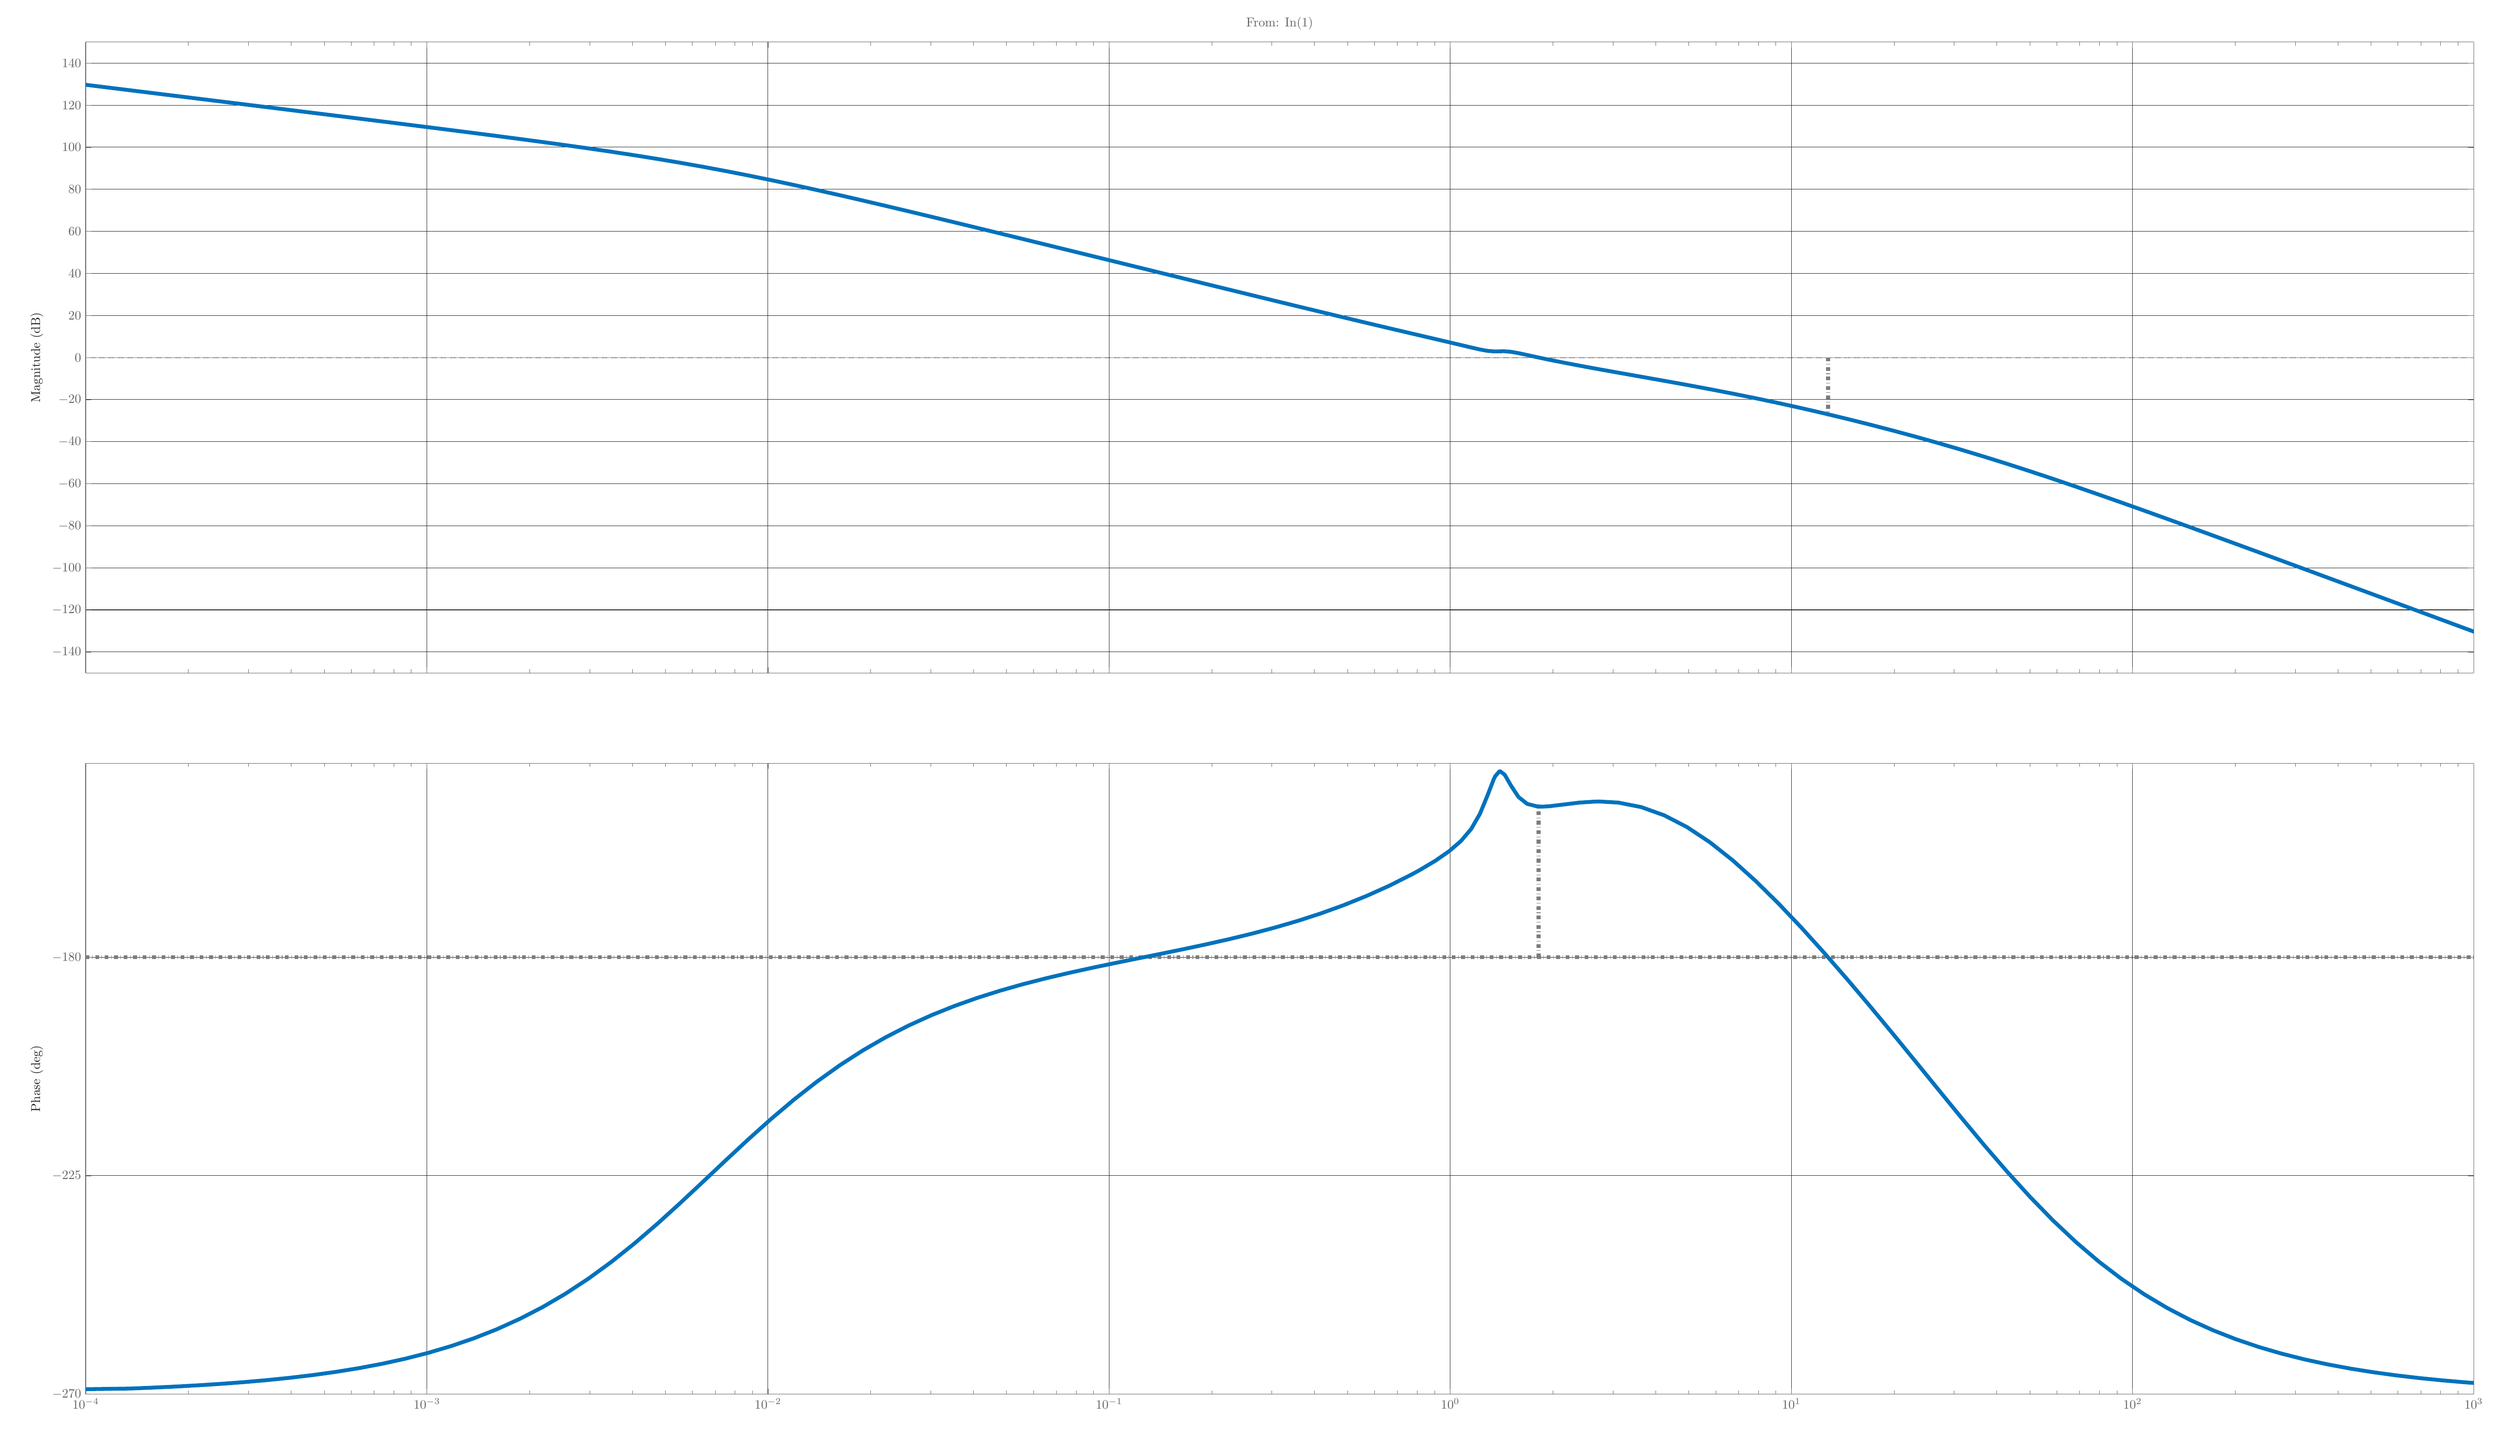
\begin{tikzpicture}

\begin{axis}[%
width=25.775in,
height=6.812in,
at={(0.787in,0.309in)},
scale only axis,
unbounded coords=jump,
separate axis lines,
every outer x axis line/.append style={mycolor3},
every x tick label/.append style={font=\color{mycolor3}},
every x tick/.append style={mycolor3},
xmode=log,
xmin=0.0001,
xmax=1000,
xminorticks=true,
every outer y axis line/.append style={mycolor3},
every y tick label/.append style={font=\color{mycolor3}},
every y tick/.append style={mycolor3},
ymin=-270,
ymax=-140,
ytick={-270, -225, -180, -135},
ylabel style={font=\color{mycolor4}},
ylabel={Phase (deg)},
axis background/.style={fill=white},
xmajorgrids,
ymajorgrids,
grid style={mycolor4}
]
\addplot [color=mycolor1, line width=1.5pt, forget plot]
  table[row sep=crcr]{%
nan	-270\\
nan	-140\\
};
\addplot [color=mycolor1, line width=1.5pt, forget plot]
  table[row sep=crcr]{%
nan	-270\\
nan	-140\\
};
\addplot [color=mycolor1, dashdotted, line width=3.0pt, forget plot]
  table[row sep=crcr]{%
0.0001	-180\\
1000	-180\\
nan	nan\\
0.0001	-360\\
1000	-360\\
nan	nan\\
};
\addplot [color=mycolor1, dashdotted, line width=3.0pt, forget plot]
  table[row sep=crcr]{%
1.81632290442861	-180\\
1.81632290442861	-148.934529454316\\
nan	nan\\
};
\addplot [color=mycolor2, line width=3.0pt, forget plot]
  table[row sep=crcr]{%
-1e+20	-270\\
-1.75e+18	-270\\
-17500000000000	-269.999999999869\\
-1750000000	-269.999998689998\\
-1750000	-269.998689997811\\
-17500	-269.868999934888\\
-1750	-268.690151607349\\
-1499.51714660695	-268.47141641764\\
-1284.88667026756	-268.216181457456\\
-1100.97691057881	-267.918372253838\\
-943.390717389296	-267.570912894969\\
-808.360318100044	-267.165566528376\\
-692.657232930092	-266.692753763957\\
-593.515084285712	-266.141347927853\\
-508.563454660737	-265.498447440201\\
-435.771211657966	-264.749127966093\\
-373.397945073603	-263.876181011176\\
-319.95235494038	-262.859852173003\\
-274.156595617355	-261.677602533766\\
-234.915723419207	-260.303932272212\\
-201.291517299815	-258.710328286304\\
-172.480046661486	-256.86542893758\\
-147.792449952265	-254.735538764358\\
-126.638464481412	-252.285669521891\\
-108.512313662772	-249.481317315947\\
-92.9806142601818	-246.291179381739\\
-79.6720145058224	-242.690918538156\\
-68.2683153463989	-238.667835958464\\
-58.4968625325115	-234.22587433322\\
-50.1240276515489	-229.389804443454\\
-42.9496222402847	-224.206996749675\\
-36.8021114226273	-218.745269451642\\
-31.5345126340395	-213.086286153324\\
-27.0208813740775	-207.31569996831\\
-23.1532999639208	-201.512872527645\\
-19.8392973122476	-195.743502336955\\
-16.9996379979133	-190.057503859892\\
-14.5664278079897	-184.492588353008\\
-12.4814904359387	-179.082192098008\\
-10.6949765279433	-173.865260909169\\
-9.16417182069131	-168.894962262243\\
-7.85247587404504	-164.243540734885\\
-6.72852698082737	-160.001321182802\\
-5.76545233094749	-156.269378689282\\
-4.940225501829	-153.147282446084\\
-4.23311591319856	-150.718676932324\\
-3.62721708309484	-149.037382412619\\
-3.10804240603791	-148.114848556016\\
-2.74056502950711	-147.89500804135\\
-2.66317878870592	-147.90557750255\\
-2.39237635077625	-148.114288382141\\
-2.14399148550879	-148.521749003766\\
-1.95196026166226	-148.869239370193\\
-1.85257528069098	-148.950654769454\\
-1.80130128659818	-148.916822245379\\
-1.68160667044661	-148.38364202748\\
-1.58548448116874	-146.964787633674\\
-1.50757886072228	-144.638268792743\\
-1.44393831174424	-142.360209541983\\
-1.40184847594141	-141.68449658122\\
-1.39159923312489	-141.73170548601\\
-1.35500109262074	-142.676500644128\\
-1.34115731252706	-143.314526313809\\
-1.28454204027906	-146.730038317009\\
-1.22142376581715	-150.454370836478\\
-1.15160605608174	-153.556312962162\\
-1.07508301917166	-156.031548071502\\
-0.992104431462472	-158.14714812826\\
-0.903244457229835	-160.128388303385\\
-0.809466464172925	-162.114831642027\\
-0.773940231521988	-162.864043504604\\
-0.663163798637812	-165.239511548265\\
-0.568243135466512	-167.358254944706\\
-0.486908757184988	-169.257281293113\\
-0.41721601727541	-170.960064462489\\
-0.357498612424878	-172.488529750255\\
-0.306328742411026	-173.86533588285\\
-0.262482972425072	-175.113758062291\\
-0.224912981625002	-176.257161397537\\
-0.192720498537819	-177.318598930176\\
-0.165135824034342	-178.320633187201\\
-0.141499428376322	-179.285354874536\\
-0.121246182334501	-180.234546539848\\
-0.103891845354981	-181.189943257465\\
-0.0890214877156746	-182.173552608925\\
-0.0762795698549222	-183.208004278202\\
-0.0653614416761475	-184.316902769909\\
-0.0560060585830474	-185.525154035592\\
-0.0479897400909444	-186.859227270563\\
-0.0411208217871896	-188.347295678058\\
-0.0352350727728339	-190.019173413125\\
-0.0301917690198903	-191.90593000507\\
-0.025870328760984	-194.03902130772\\
-0.0221674294659739	-196.448737731075\\
-0.0189945374745302	-199.16175982253\\
-0.0162757912199579	-202.197671187736\\
-0.0139461874336695	-205.564470163959\\
-0.011950026963761	-209.253499535564\\
-0.0102395830483285	-213.234764236745\\
-0.00877396020289968	-217.454156371418\\
-0.00751811643879716	-221.834280349041\\
-0.00644202543437937	-226.279948942085\\
-0.00551995862727425	-230.687932520432\\
-0.00472987006294781	-234.958796057717\\
-0.00405286929177892	-239.007697574398\\
-0.00347276971198814	-242.771505634551\\
-0.00297570155962485	-246.21118487169\\
-0.00254978029248142	-249.310081939664\\
-0.00218482243923221	-252.069692741589\\
-0.00187210211995446	-254.504556819848\\
-0.00160414241661196	-256.637455932259\\
-0.00137453660531951	-258.495513023294\\
-0.00117779497618029	-260.107341557575\\
-0.00100921357826849	-261.501142917718\\
-0.000864761751544091	-262.703551030775\\
-0.000740985756668696	-263.739015364013\\
-0.000634926198580705	-264.629545797611\\
-0.000544047269486705	-265.394685829973\\
-0.000466176119520002	-266.05162003716\\
-0.000399450905462247	-266.61535293116\\
-0.000342276275410463	-267.098919079162\\
-0.000293285225059857	-267.513599996117\\
-0.000251306413613562	-267.869133681588\\
-0.00021533615786619	-268.173909305595\\
-0.000184514434859893	-268.435143664702\\
-0.000158104319353657	-268.659038495425\\
-0.000135474364470531	-268.850919141354\\
-1.35474364470531e-05	-269.885076791714\\
-1.35474364470531e-07	-269.998850766389\\
-1.35474364470531e-10	-269.999998850766\\
-1.35474364470531e-14	-269.999999999885\\
-1.35474364470531e-19	-270\\
-1e-20	-270\\
1e-20	-270\\
1.35474364470531e-19	-270\\
1.35474364470531e-14	-269.999999999885\\
1.35474364470531e-10	-269.999998850766\\
1.35474364470531e-07	-269.998850766389\\
1.35474364470531e-05	-269.885076791714\\
0.000135474364470531	-268.850919141354\\
0.000158104319353657	-268.659038495425\\
0.000184514434859893	-268.435143664702\\
0.00021533615786619	-268.173909305595\\
0.000251306413613562	-267.869133681588\\
0.000293285225059857	-267.513599996117\\
0.000342276275410463	-267.098919079162\\
0.000399450905462247	-266.61535293116\\
0.000466176119520002	-266.05162003716\\
0.000544047269486705	-265.394685829973\\
0.000634926198580705	-264.629545797611\\
0.000740985756668696	-263.739015364013\\
0.000864761751544091	-262.703551030775\\
0.00100921357826849	-261.501142917718\\
0.00117779497618029	-260.107341557575\\
0.00137453660531951	-258.495513023294\\
0.00160414241661196	-256.637455932259\\
0.00187210211995446	-254.504556819848\\
0.00218482243923221	-252.069692741589\\
0.00254978029248142	-249.310081939664\\
0.00297570155962485	-246.21118487169\\
0.00347276971198814	-242.771505634551\\
0.00405286929177892	-239.007697574398\\
0.00472987006294781	-234.958796057717\\
0.00551995862727425	-230.687932520432\\
0.00644202543437937	-226.279948942085\\
0.00751811643879716	-221.834280349041\\
0.00877396020289968	-217.454156371418\\
0.0102395830483285	-213.234764236745\\
0.011950026963761	-209.253499535564\\
0.0139461874336695	-205.564470163959\\
0.0162757912199579	-202.197671187736\\
0.0189945374745302	-199.16175982253\\
0.0221674294659739	-196.448737731075\\
0.025870328760984	-194.03902130772\\
0.0301917690198903	-191.90593000507\\
0.0352350727728339	-190.019173413125\\
0.0411208217871896	-188.347295678058\\
0.0479897400909444	-186.859227270563\\
0.0560060585830474	-185.525154035592\\
0.0653614416761475	-184.316902769909\\
0.0762795698549222	-183.208004278202\\
0.0890214877156746	-182.173552608925\\
0.103891845354981	-181.189943257465\\
0.121246182334501	-180.234546539848\\
0.141499428376322	-179.285354874536\\
0.165135824034342	-178.320633187201\\
0.192720498537819	-177.318598930176\\
0.224912981625002	-176.257161397537\\
0.262482972425072	-175.113758062291\\
0.306328742411026	-173.86533588285\\
0.357498612424878	-172.488529750255\\
0.41721601727541	-170.960064462489\\
0.486908757184988	-169.257281293113\\
0.568243135466512	-167.358254944706\\
0.663163798637812	-165.239511548265\\
0.773940231521988	-162.864043504604\\
0.809466464172925	-162.114831642027\\
0.903244457229835	-160.128388303385\\
0.992104431462472	-158.14714812826\\
1.07508301917166	-156.031548071502\\
1.15160605608174	-153.556312962162\\
1.22142376581715	-150.454370836478\\
1.28454204027906	-146.730038317009\\
1.34115731252706	-143.314526313809\\
1.35500109262074	-142.676500644128\\
1.39159923312489	-141.73170548601\\
1.40184847594141	-141.68449658122\\
1.44393831174424	-142.360209541983\\
1.50757886072228	-144.638268792743\\
1.58548448116874	-146.964787633674\\
1.68160667044661	-148.38364202748\\
1.80130128659818	-148.916822245379\\
1.85257528069098	-148.950654769454\\
1.95196026166226	-148.869239370193\\
2.14399148550879	-148.521749003766\\
2.39237635077625	-148.114288382141\\
2.66317878870592	-147.90557750255\\
2.74056502950711	-147.89500804135\\
3.10804240603791	-148.114848556016\\
3.62721708309484	-149.037382412619\\
4.23311591319856	-150.718676932324\\
4.940225501829	-153.147282446084\\
5.76545233094749	-156.269378689282\\
6.72852698082737	-160.001321182802\\
7.85247587404504	-164.243540734885\\
9.16417182069131	-168.894962262243\\
10.6949765279433	-173.865260909169\\
12.4814904359387	-179.082192098008\\
14.5664278079897	-184.492588353008\\
16.9996379979133	-190.057503859892\\
19.8392973122476	-195.743502336955\\
23.1532999639208	-201.512872527645\\
27.0208813740775	-207.31569996831\\
31.5345126340395	-213.086286153324\\
36.8021114226273	-218.745269451642\\
42.9496222402847	-224.206996749675\\
50.1240276515489	-229.389804443454\\
58.4968625325115	-234.22587433322\\
68.2683153463989	-238.667835958464\\
79.6720145058224	-242.690918538156\\
92.9806142601818	-246.291179381739\\
108.512313662772	-249.481317315947\\
126.638464481412	-252.285669521891\\
147.792449952265	-254.735538764358\\
172.480046661486	-256.86542893758\\
201.291517299815	-258.710328286304\\
234.915723419207	-260.303932272212\\
274.156595617355	-261.677602533766\\
319.95235494038	-262.859852173003\\
373.397945073603	-263.876181011176\\
435.771211657966	-264.749127966093\\
508.563454660737	-265.498447440201\\
593.515084285712	-266.141347927853\\
692.657232930092	-266.692753763957\\
808.360318100044	-267.165566528376\\
943.390717389296	-267.570912894969\\
1100.97691057881	-267.918372253838\\
1284.88667026756	-268.216181457456\\
1499.51714660695	-268.47141641764\\
1750	-268.690151607349\\
17500	-269.868999934888\\
1750000	-269.998689997811\\
1750000000	-269.999998689998\\
17500000000000	-269.999999999869\\
1.75e+18	-270\\
1e+20	-270\\
};
\addplot[only marks, mark=*, mark options={}, mark size=1.5000pt, draw=mycolor2, fill=white, forget plot] table[row sep=crcr]{%
x	y\\
nan	nan\\
};
\addplot[only marks, mark=*, mark options={}, mark size=1.5000pt, draw=mycolor2, fill=mycolor2, forget plot] table[row sep=crcr]{%
x	y\\
1.81632290442861	-148.92683280529\\
};
\end{axis}

\begin{axis}[%
width=25.775in,
height=6.812in,
at={(0.787in,8.095in)},
scale only axis,
unbounded coords=jump,
separate axis lines,
every outer x axis line/.append style={mycolor3},
every x tick label/.append style={font=\color{mycolor3}},
every x tick/.append style={mycolor3},
xmode=log,
xmin=0.0001,
xmax=1000,
xtick={0.0001,0.001,0.01,0.1,1,10,100,1000},
xticklabels={\empty},
xminorticks=true,
every outer y axis line/.append style={mycolor3},
every y tick label/.append style={font=\color{mycolor3}},
every y tick/.append style={mycolor3},
ymin=-150,
ymax=150,
ylabel style={font=\color{mycolor4}},
ylabel={Magnitude (dB)},
axis background/.style={fill=white},
title style={font=\color{mycolor3}},
title={From: In(1)},
xmajorgrids,
ymajorgrids,
grid style={mycolor4}
]
\addplot [color=mycolor1, line width=1.5pt, forget plot]
  table[row sep=crcr]{%
nan	-150\\
nan	150\\
};
\addplot [color=mycolor1, line width=1.5pt, forget plot]
  table[row sep=crcr]{%
nan	-150\\
nan	150\\
};
\addplot [color=mycolor1, dashdotted, forget plot]
  table[row sep=crcr]{%
0.0001	0\\
1000	0\\
};
\addplot [color=mycolor1, dashdotted, line width=3.0pt, forget plot]
  table[row sep=crcr]{%
12.8174681266129	0\\
12.8174681266129	-26.9991681943771\\
nan	nan\\
};
\addplot [color=mycolor2, line width=3.0pt, forget plot]
  table[row sep=crcr]{%
-1e+20	-1150.29410569715\\
-1.75e+18	-1044.87638861833\\
-17500000000000	-744.876388618331\\
-1750000000	-504.876388618332\\
-1750000	-324.876388620128\\
-17500	-204.876406580418\\
-1750	-144.878184482663\\
-1499.51714660695	-140.853637641516\\
-1284.88667026756	-136.829325913248\\
-1100.97691057881	-132.80533428072\\
-943.390717389296	-128.781778382728\\
-808.360318100044	-124.75881552\\
-692.657232930092	-120.736659567739\\
-593.515084285712	-116.715601143186\\
-508.563454660737	-112.696034809558\\
-435.771211657966	-108.678495641414\\
-373.397945073603	-104.663708133968\\
-319.95235494038	-100.652651185178\\
-274.156595617355	-96.6466436316643\\
-234.915723419207	-92.6474553838459\\
-201.291517299815	-88.6574491927859\\
-172.480046661486	-84.6797567840698\\
-147.792449952265	-80.7184893447732\\
-126.638464481412	-76.7789744324475\\
-108.512313662772	-72.8679972051802\\
-92.9806142601818	-68.9940018639138\\
-79.6720145058224	-65.1671804407882\\
-68.2683153463989	-61.3993481397212\\
-58.4968625325115	-57.7034955442041\\
-50.1240276515489	-54.0929463676794\\
-42.9496222402847	-50.5801592716091\\
-36.8021114226273	-47.1753831691752\\
-31.5345126340395	-43.8855343248762\\
-27.0208813740775	-40.7136940329242\\
-23.1532999639208	-37.6594547404414\\
-19.8392973122476	-34.7200281745745\\
-16.9996379979133	-31.8917385238749\\
-14.5664278079897	-29.1714015456699\\
-12.4814904359387	-26.5571562868036\\
-10.6949765279433	-24.0484927241734\\
-9.16417182069131	-21.6454289304891\\
-7.85247587404504	-19.3470052235496\\
-6.72852698082737	-17.1494615642079\\
-5.76545233094749	-15.0445883431843\\
-4.940225501829	-13.0187008000824\\
-4.23311591319856	-11.0524518113873\\
-3.62721708309484	-9.12135055573138\\
-3.10804240603791	-7.19651445353129\\
-2.74056502950711	-5.61041610052026\\
-2.66317878870592	-5.24479665353128\\
-2.39237635077625	-3.85363021279085\\
-2.14399148550879	-2.38109398928963\\
-1.95196026166226	-1.06186971514181\\
-1.85257528069098	-0.296176256325292\\
-1.80130128659818	0.125533381248428\\
-1.68160667044661	1.18574372242419\\
-1.58548448116874	2.08399061483029\\
-1.50757886072228	2.7173011387487\\
-1.44393831174424	2.97445591373086\\
-1.40184847594141	2.96585118634296\\
-1.39159923312489	2.95171976949777\\
-1.35500109262074	2.91926770730467\\
-1.34115731252706	2.93022274343795\\
-1.28454204027906	3.19143007283507\\
-1.22142376581715	3.84038209687377\\
-1.15160605608174	4.78359023691886\\
-1.07508301917166	5.93410918165409\\
-0.992104431462472	7.2721764542705\\
-0.903244457229835	8.8203030529825\\
-0.809466464172925	10.6216572885964\\
-0.773940231521988	11.3598116445421\\
-0.663163798637812	13.9112826772728\\
-0.568243135466512	16.4846944966451\\
-0.486908757184988	19.0804545209005\\
-0.41721601727541	21.6957756527323\\
-0.357498612424878	24.3270820192554\\
-0.306328742411026	26.9709486164086\\
-0.262482972425072	29.6244229121004\\
-0.224912981625002	32.2850821058534\\
-0.192720498537819	34.9509820785287\\
-0.165135824034342	37.6205682953084\\
-0.141499428376322	40.2925792199853\\
-0.121246182334501	42.9659537975163\\
-0.103891845354981	45.639745394337\\
-0.0890214877156746	48.3130401762937\\
-0.0762795698549222	50.9848757602749\\
-0.0653614416761475	53.6541548645053\\
-0.0560060585830474	56.3195480387174\\
-0.0479897400909444	58.9793792223498\\
-0.0411208217871896	61.6314880260062\\
-0.0352350727728339	64.2730637832218\\
-0.0301917690198903	66.9004495544502\\
-0.025870328760984	69.5089209155058\\
-0.0221674294659739	72.0924565537748\\
-0.0189945374745302	74.6435373749274\\
-0.0162757912199579	77.1530382076737\\
-0.0139461874336695	79.6103064957677\\
-0.011950026963761	82.0035414057635\\
-0.0102395830483285	84.3205690422327\\
-0.00877396020289968	86.5500263839504\\
-0.00751811643879716	88.6828119622224\\
-0.00644202543437937	90.7134843922003\\
-0.00551995862727425	92.6411975273362\\
-0.00472987006294781	94.4698521012153\\
-0.00405286929177892	96.2074088537972\\
-0.00347276971198814	97.8646052356741\\
-0.00297570155962485	99.4534785031965\\
-0.00254978029248142	100.986062249828\\
-0.00218482243923221	102.473462245305\\
-0.00187210211995446	103.925345945783\\
-0.00160414241661196	105.349770392653\\
-0.00137453660531951	106.753235397289\\
-0.00117779497618029	108.140858422138\\
-0.00100921357826849	109.516596080468\\
-0.000864761751544091	110.883466435007\\
-0.000740985756668696	112.243748690562\\
-0.000634926198580705	113.599151366175\\
-0.000544047269486705	114.950948196667\\
-0.000466176119520002	116.300084950769\\
-0.000399450905462247	117.647261791684\\
-0.000342276275410463	118.992995924666\\
-0.000293285225059857	120.337668790635\\
-0.000251306413613562	121.681561370938\\
-0.00021533615786619	123.024880465239\\
-0.000184514434859893	124.367778178899\\
-0.000158104319353657	125.710366335975\\
-0.000135474364470531	127.052727118364\\
-1.35474364470531e-05	147.054446554777\\
-1.35474364470531e-07	187.054463924558\\
-1.35474364470531e-10	247.054463926295\\
-1.35474364470531e-14	327.054463926295\\
-1.35474364470531e-19	427.054463926295\\
-1e-20	449.691606373338\\
1e-20	449.691606373338\\
1.35474364470531e-19	427.054463926295\\
1.35474364470531e-14	327.054463926295\\
1.35474364470531e-10	247.054463926295\\
1.35474364470531e-07	187.054463924558\\
1.35474364470531e-05	147.054446554777\\
0.000135474364470531	127.052727118364\\
0.000158104319353657	125.710366335975\\
0.000184514434859893	124.367778178899\\
0.00021533615786619	123.024880465239\\
0.000251306413613562	121.681561370938\\
0.000293285225059857	120.337668790635\\
0.000342276275410463	118.992995924666\\
0.000399450905462247	117.647261791684\\
0.000466176119520002	116.300084950769\\
0.000544047269486705	114.950948196667\\
0.000634926198580705	113.599151366175\\
0.000740985756668696	112.243748690562\\
0.000864761751544091	110.883466435007\\
0.00100921357826849	109.516596080468\\
0.00117779497618029	108.140858422138\\
0.00137453660531951	106.753235397289\\
0.00160414241661196	105.349770392653\\
0.00187210211995446	103.925345945783\\
0.00218482243923221	102.473462245305\\
0.00254978029248142	100.986062249828\\
0.00297570155962485	99.4534785031965\\
0.00347276971198814	97.8646052356741\\
0.00405286929177892	96.2074088537972\\
0.00472987006294781	94.4698521012153\\
0.00551995862727425	92.6411975273362\\
0.00644202543437937	90.7134843922003\\
0.00751811643879716	88.6828119622224\\
0.00877396020289968	86.5500263839504\\
0.0102395830483285	84.3205690422327\\
0.011950026963761	82.0035414057635\\
0.0139461874336695	79.6103064957677\\
0.0162757912199579	77.1530382076737\\
0.0189945374745302	74.6435373749274\\
0.0221674294659739	72.0924565537748\\
0.025870328760984	69.5089209155058\\
0.0301917690198903	66.9004495544502\\
0.0352350727728339	64.2730637832218\\
0.0411208217871896	61.6314880260062\\
0.0479897400909444	58.9793792223498\\
0.0560060585830474	56.3195480387174\\
0.0653614416761475	53.6541548645053\\
0.0762795698549222	50.9848757602749\\
0.0890214877156746	48.3130401762937\\
0.103891845354981	45.639745394337\\
0.121246182334501	42.9659537975163\\
0.141499428376322	40.2925792199853\\
0.165135824034342	37.6205682953084\\
0.192720498537819	34.9509820785287\\
0.224912981625002	32.2850821058534\\
0.262482972425072	29.6244229121004\\
0.306328742411026	26.9709486164086\\
0.357498612424878	24.3270820192554\\
0.41721601727541	21.6957756527323\\
0.486908757184988	19.0804545209005\\
0.568243135466512	16.4846944966451\\
0.663163798637812	13.9112826772728\\
0.773940231521988	11.3598116445421\\
0.809466464172925	10.6216572885964\\
0.903244457229835	8.8203030529825\\
0.992104431462472	7.2721764542705\\
1.07508301917166	5.93410918165409\\
1.15160605608174	4.78359023691886\\
1.22142376581715	3.84038209687377\\
1.28454204027906	3.19143007283507\\
1.34115731252706	2.93022274343795\\
1.35500109262074	2.91926770730467\\
1.39159923312489	2.95171976949777\\
1.40184847594141	2.96585118634296\\
1.44393831174424	2.97445591373086\\
1.50757886072228	2.7173011387487\\
1.58548448116874	2.08399061483029\\
1.68160667044661	1.18574372242419\\
1.80130128659818	0.125533381248428\\
1.85257528069098	-0.296176256325292\\
1.95196026166226	-1.06186971514181\\
2.14399148550879	-2.38109398928963\\
2.39237635077625	-3.85363021279085\\
2.66317878870592	-5.24479665353128\\
2.74056502950711	-5.61041610052026\\
3.10804240603791	-7.19651445353129\\
3.62721708309484	-9.12135055573138\\
4.23311591319856	-11.0524518113873\\
4.940225501829	-13.0187008000824\\
5.76545233094749	-15.0445883431843\\
6.72852698082737	-17.1494615642079\\
7.85247587404504	-19.3470052235496\\
9.16417182069131	-21.6454289304891\\
10.6949765279433	-24.0484927241734\\
12.4814904359387	-26.5571562868036\\
14.5664278079897	-29.1714015456699\\
16.9996379979133	-31.8917385238749\\
19.8392973122476	-34.7200281745745\\
23.1532999639208	-37.6594547404414\\
27.0208813740775	-40.7136940329242\\
31.5345126340395	-43.8855343248762\\
36.8021114226273	-47.1753831691752\\
42.9496222402847	-50.5801592716091\\
50.1240276515489	-54.0929463676794\\
58.4968625325115	-57.7034955442041\\
68.2683153463989	-61.3993481397212\\
79.6720145058224	-65.1671804407882\\
92.9806142601818	-68.9940018639138\\
108.512313662772	-72.8679972051802\\
126.638464481412	-76.7789744324475\\
147.792449952265	-80.7184893447732\\
172.480046661486	-84.6797567840698\\
201.291517299815	-88.6574491927859\\
234.915723419207	-92.6474553838459\\
274.156595617355	-96.6466436316643\\
319.95235494038	-100.652651185178\\
373.397945073603	-104.663708133968\\
435.771211657966	-108.678495641414\\
508.563454660737	-112.696034809558\\
593.515084285712	-116.715601143186\\
692.657232930092	-120.736659567739\\
808.360318100044	-124.75881552\\
943.390717389296	-128.781778382728\\
1100.97691057881	-132.80533428072\\
1284.88667026756	-136.829325913248\\
1499.51714660695	-140.853637641516\\
1750	-144.878184482663\\
17500	-204.876406580418\\
1750000	-324.876388620128\\
1750000000	-504.876388618332\\
17500000000000	-744.876388618331\\
1.75e+18	-1044.87638861833\\
1e+20	-1150.29410569715\\
};
\addplot[only marks, mark=*, mark options={}, mark size=1.5000pt, draw=mycolor2, fill=white, forget plot] table[row sep=crcr]{%
x	y\\
nan	nan\\
};
\addplot[only marks, mark=*, mark options={}, mark size=1.5000pt, draw=mycolor2, fill=mycolor2, forget plot] table[row sep=crcr]{%
x	y\\
12.8174681266129	-26.9991681943771\\
};
\end{axis}

\begin{axis}[%
width=26.667in,
height=15in,
at={(0in,0in)},
scale only axis,
xmin=0,
xmax=1,
ymin=0,
ymax=1,
axis line style={draw=none},
ticks=none,
axis x line*=bottom,
axis y line*=left
]
\end{axis}
\end{tikzpicture}%}
\caption{Design B analysis: (left) Root locus showing reduced damping from integral action; (right) Bode plot with PM = 38°.}
\label{fig:design_B_rlocus}
\label{fig:design_B_bode}
\end{figure}

\begin{figure}[h!]
\centering
\resizebox{0.7\textwidth}{!}{% This file was created by matlab2tikz.
%
\definecolor{mycolor1}{rgb}{0.49020,0.49020,0.49020}%
\definecolor{mycolor2}{rgb}{0.00000,0.44700,0.74100}%
\definecolor{mycolor3}{rgb}{0.38039,0.38039,0.38039}%
\definecolor{mycolor4}{rgb}{0.12941,0.12941,0.12941}%
%
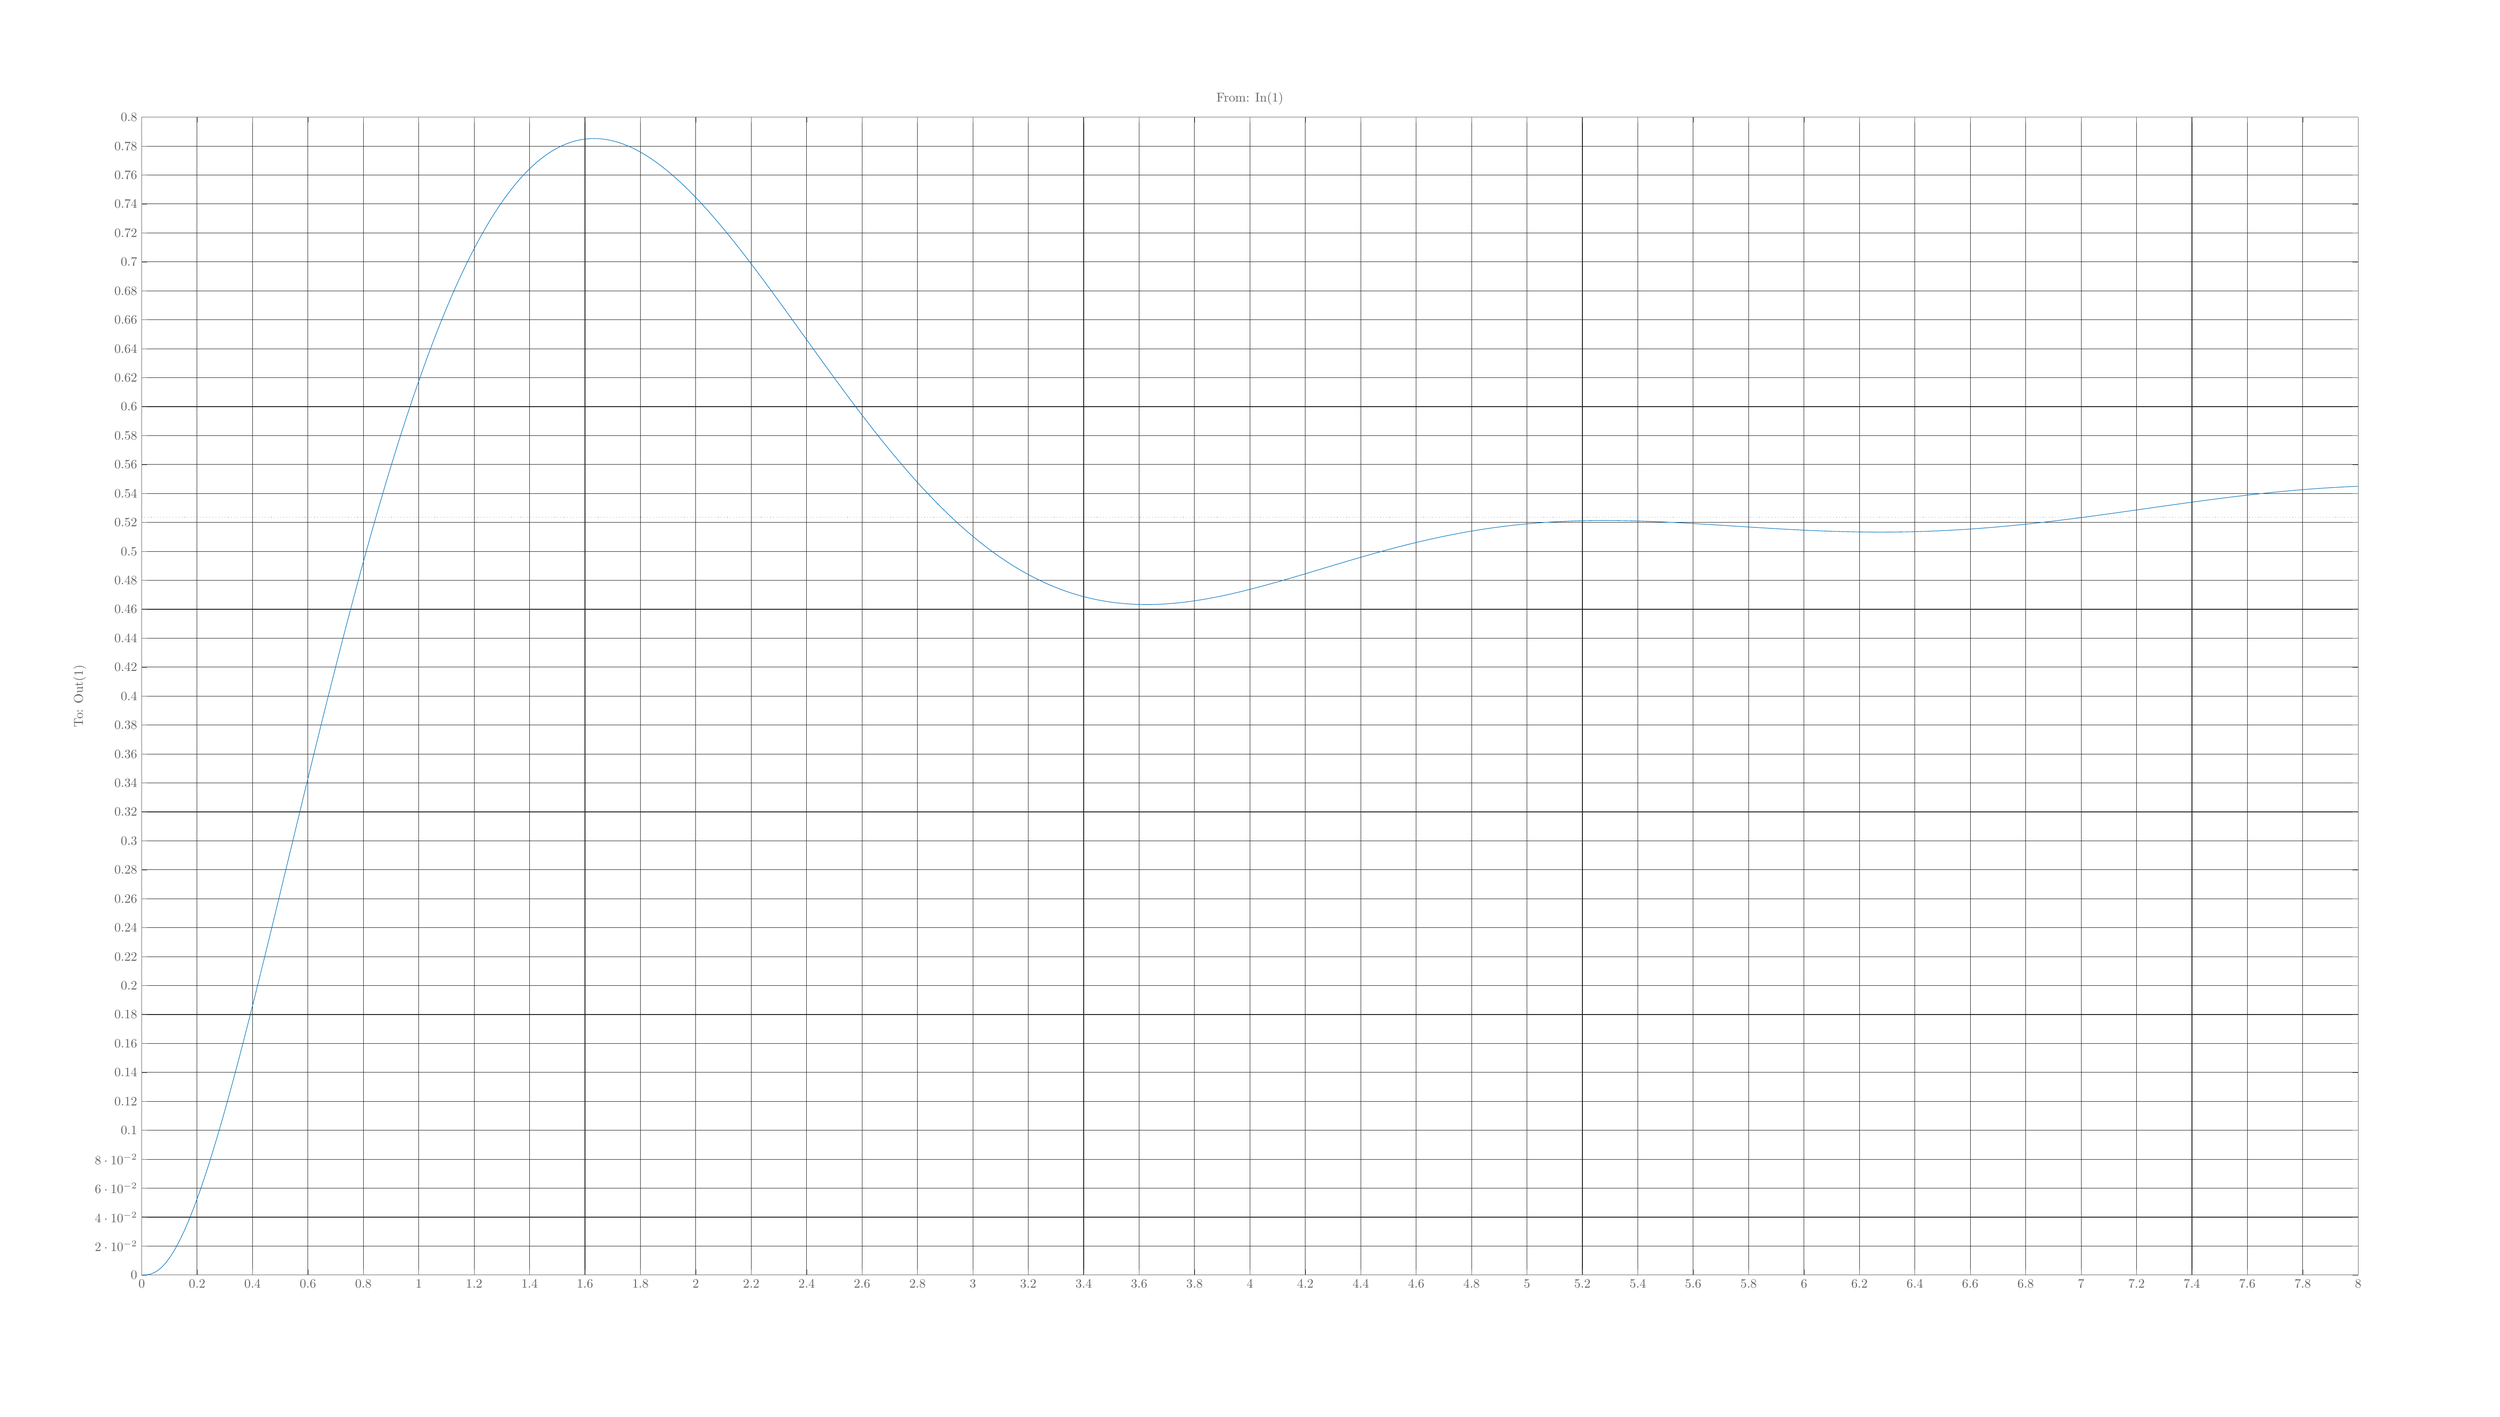
\begin{tikzpicture}

\begin{axis}[%
width=23.889in,
height=12.486in,
at={(1.389in,1.389in)},
scale only axis,
separate axis lines,
every outer x axis line/.append style={mycolor3},
every x tick label/.append style={font=\color{mycolor3}},
every x tick/.append style={mycolor3},
xmin=0,
xmax=8,
every outer y axis line/.append style={mycolor3},
every y tick label/.append style={font=\color{mycolor3}},
every y tick/.append style={mycolor3},
ymin=0,
ymax=0.8,
ylabel style={font=\color{mycolor3}},
ylabel={To: Out(1)},
axis background/.style={fill=white},
title style={font=\color{mycolor3}},
title={From: In(1)},
xmajorgrids,
ymajorgrids,
grid style={mycolor4}
]
\addplot [color=mycolor1, dotted, forget plot]
  table[row sep=crcr]{%
0	0.523598775598299\\
8	0.523598775598299\\
};
\addplot [color=mycolor2, forget plot]
  table[row sep=crcr]{%
0	0\\
0.0172043010752688	0.000115083225951973\\
0.0344086021505376	0.000789072739332498\\
0.0516129032258065	0.00230658169995276\\
0.0688172043010753	0.00478039242505776\\
0.0860215053763441	0.00823279363115475\\
0.103225806451613	0.0126396329948798\\
0.120430107526882	0.0179540766214954\\
0.137634408602151	0.024119332366227\\
0.154838709677419	0.0310753793678662\\
0.172043010752688	0.0387624497070007\\
0.189247311827957	0.047122756874218\\
0.206451612903226	0.0561012840557729\\
0.223655913978495	0.0656460739134277\\
0.240860215053763	0.0757082593077412\\
0.258064516129032	0.086241964324275\\
0.275268817204301	0.0972041450706343\\
0.29247311827957	0.108554407166129\\
0.309677419354839	0.120254819192911\\
0.326881720430108	0.132269731832901\\
0.344086021505376	0.144565607282145\\
0.361290322580645	0.157110860799657\\
0.378494623655914	0.169875714814531\\
0.395698924731183	0.182832065285971\\
0.412903225806452	0.195953359660795\\
0.43010752688172	0.209214485625453\\
0.447311827956989	0.222591669808464\\
0.464516129032258	0.236062385602737\\
0.481720430107527	0.249605269317347\\
0.498924731182796	0.263200043920063\\
0.516129032258065	0.276827449687388\\
0.533333333333333	0.290469181133915\\
0.550537634408602	0.304107829645527\\
0.567741935483871	0.317726831290335\\
0.58494623655914	0.331310419327057\\
0.602150537634409	0.344843580972735\\
0.619354838709677	0.358312018030344\\
0.636559139784946	0.371702111012281\\
0.653763440860215	0.385000886428116\\
0.670967741935484	0.398195986934535\\
0.688172043010753	0.411275644072427\\
0.705376344086021	0.424228653340703\\
0.72258064516129	0.43704435137895\\
0.739784946236559	0.449712595051531\\
0.756989247311828	0.462223742244486\\
0.774193548387097	0.474568634203697\\
0.791397849462366	0.486738579258354\\
0.808602150537634	0.498725337788016\\
0.825806451612903	0.510521108304559\\
0.843010752688172	0.522118514532117\\
0.860215053763441	0.533510593379006\\
0.87741935483871	0.544690783705426\\
0.894623655913979	0.555652915799794\\
0.911827956989247	0.566391201484767\\
0.929032258064516	0.576900224781497\\
0.946236559139785	0.58717493306755\\
0.963440860215054	0.597210628670126\\
0.980645161290323	0.607002960841938\\
0.997849462365591	0.616547918072305\\
1.01505376344086	0.625841820690774\\
1.03225806451613	0.63488131372487\\
1.0494623655914	0.643663359977594\\
1.06666666666667	0.652185233293818\\
1.08387096774194	0.660444511988056\\
1.1010752688172	0.668439072409078\\
1.11827956989247	0.676167082619548\\
1.13548387096774	0.683626996171378\\
1.15268817204301	0.690817545959732\\
1.16989247311828	0.697737738140716\\
1.18709677419355	0.704386846099627\\
1.20430107526882	0.71076440445838\\
1.22150537634409	0.716870203112286\\
1.23870967741935	0.722704281287737\\
1.25591397849462	0.728266921613702\\
1.27311827956989	0.733558644201042\\
1.29032258064516	0.738580200724757\\
1.30752688172043	0.743332568505226\\
1.3247311827957	0.747816944585369\\
1.34193548387097	0.752034739801445\\
1.35913978494624	0.755987572845932\\
1.37634408602151	0.759677264321546\\
1.39354838709677	0.763105830786061\\
1.41075268817204	0.766275478788095\\
1.42795698924731	0.76918859889451\\
1.44516129032258	0.771847759710459\\
1.46236559139785	0.774255701893529\\
1.47956989247312	0.776415332163714\\
1.49677419354839	0.778329717311279\\
1.51397849462366	0.780002078204807\\
1.53118279569892	0.781435783801966\\
1.54838709677419	0.782634345165709\\
1.56559139784946	0.783601409488805\\
1.58279569892473	0.784340754129737\\
1.6	0.784856280663106\\
1.61720430107527	0.785152008947815\\
1.63440860215054	0.785232071216349\\
1.65161290322581	0.785100706188555\\
1.66881720430108	0.78476225321336\\
1.68602150537634	0.784221146441895\\
1.70322580645161	0.783481909035525\\
1.72043010752688	0.782549147412261\\
1.73763440860215	0.781427545535052\\
1.75483870967742	0.780121859245421\\
1.77204301075269	0.778636910645879\\
1.78924731182796	0.776977582534525\\
1.80645161290323	0.775148812895193\\
1.82365591397849	0.773155589446437\\
1.84086021505376	0.771002944252609\\
1.85806451612903	0.768695948400218\\
1.8752688172043	0.766239706742648\\
1.89247311827957	0.763639352716308\\
1.90967741935484	0.760900043231121\\
1.92688172043011	0.758026953638249\\
1.94408602150538	0.755025272777806\\
1.96129032258065	0.751900198109257\\
1.97849462365591	0.748656930927073\\
1.99569892473118	0.745300671664138\\
2.01290322580645	0.741836615285286\\
2.03010752688172	0.738269946773261\\
2.04731182795699	0.734605836709254\\
2.06451612903226	0.730849436950111\\
2.08172043010753	0.727005876404156\\
2.0989247311828	0.723080256907482\\
2.11612903225806	0.719077649202463\\
2.13333333333333	0.715003089020102\\
2.1505376344086	0.71086157326774\\
2.16774193548387	0.70665805632354\\
2.18494623655914	0.702397446439033\\
2.20215053763441	0.69808460225091\\
2.21935483870968	0.693724329403144\\
2.23655913978495	0.689321377280387\\
2.25376344086022	0.68488043585351\\
2.27096774193548	0.680406132638018\\
2.28817204301075	0.67590302976597\\
2.30537634408602	0.671375621171942\\
2.32258064516129	0.666828329893435\\
2.33978494623656	0.662265505486049\\
2.35698924731183	0.657691421553633\\
2.3741935483871	0.6531102733935\\
2.39139784946237	0.648526175756725\\
2.40860215053763	0.64394316072342\\
2.4258064516129	0.63936517569279\\
2.44301075268817	0.634796081487672\\
2.46021505376344	0.630239650573177\\
2.47741935483871	0.625699565388937\\
2.49462365591398	0.6211794167944\\
2.51182795698925	0.616682702626496\\
2.52903225806452	0.612212826368923\\
2.54623655913979	0.60777309593222\\
2.56344086021505	0.603366722543712\\
2.58064516129032	0.598996819746303\\
2.59784946236559	0.594666402505062\\
2.61505376344086	0.590378386420428\\
2.63225806451613	0.586135587046806\\
2.6494623655914	0.581940719315247\\
2.66666666666667	0.577796397058845\\
2.68387096774194	0.573705132639393\\
2.7010752688172	0.569669336673819\\
2.71827956989247	0.56569131785879\\
2.73548387096774	0.561773282891906\\
2.75268817204301	0.557917336487744\\
2.76989247311828	0.55412548148705\\
2.78709677419355	0.550399619057262\\
2.80430107526882	0.546741548982522\\
2.82150537634409	0.54315297004128\\
2.83870967741935	0.539635480469568\\
2.85591397849462	0.536190578507927\\
2.87311827956989	0.532819663030008\\
2.89032258064516	0.529524034250747\\
2.90752688172043	0.526304894512041\\
2.9247311827957	0.523163349143794\\
2.94193548387097	0.520100407398166\\
2.95913978494624	0.517116983454838\\
2.97634408602151	0.514213897495095\\
2.99354838709677	0.511391876842467\\
3.01075268817204	0.50865155716769\\
3.02795698924731	0.505993483755705\\
3.04516129032258	0.503418112832405\\
3.06236559139785	0.500925812948818\\
3.07956989247312	0.498516866420421\\
3.09677419354839	0.49619147081925\\
3.11397849462366	0.493949740516476\\
3.13118279569892	0.491791708273112\\
3.14838709677419	0.489717326876505\\
3.16559139784946	0.487726470820281\\
3.18279569892473	0.485818938025391\\
3.2	0.48399445159994\\
3.21720430107527	0.482252661635455\\
3.23440860215054	0.480593147037278\\
3.25161290322581	0.479015417386769\\
3.26881720430108	0.477518914833018\\
3.28602150537634	0.47610301601179\\
3.30322580645161	0.474767033989406\\
3.32043010752688	0.473510220229343\\
3.33763440860215	0.472331766579278\\
3.35483870967742	0.471230807276395\\
3.37204301075269	0.470206420968735\\
3.38924731182796	0.469257632750441\\
3.40645161290323	0.46838341620874\\
3.42365591397849	0.467582695480554\\
3.44086021505376	0.466854347316649\\
3.45806451612903	0.466197203151256\\
3.4752688172043	0.465610051175146\\
3.49247311827957	0.465091638410164\\
3.50967741935484	0.464640672783247\\
3.52688172043011	0.464255825198011\\
3.54408602150538	0.463935731602017\\
3.56129032258065	0.463678995047845\\
3.57849462365591	0.463484187746183\\
3.59569892473118	0.463349853109133\\
3.61290322580645	0.463274507782013\\
3.63010752688172	0.463256643661945\\
3.64731182795699	0.463294729901584\\
3.66451612903226	0.463387214896373\\
3.68172043010753	0.463532528253752\\
3.6989247311828	0.463729082742802\\
3.71612903225806	0.463975276222833\\
3.73333333333333	0.464269493549503\\
3.7505376344086	0.46461010845704\\
3.76774193548387	0.464995485415274\\
3.78494623655914	0.465423981460132\\
3.80215053763441	0.465893947996381\\
3.81935483870968	0.466403732571406\\
3.83655913978495	0.466951680618858\\
3.85376344086021	0.467536137171084\\
3.87096774193548	0.468155448539261\\
3.88817204301075	0.468807963960241\\
3.90537634408602	0.469492037209128\\
3.92258064516129	0.470206028176683\\
3.93978494623656	0.470948304410694\\
3.95698924731183	0.471717242620478\\
3.9741935483871	0.472511230143769\\
3.99139784946237	0.473328666375249\\
4.00860215053763	0.474167964156062\\
4.0258064516129	0.475027551123683\\
4.04301075268817	0.475905871021565\\
4.06021505376344	0.476801384968031\\
4.07741935483871	0.477712572683927\\
4.09462365591398	0.478637933678612\\
4.11182795698925	0.479575988393871\\
4.12903225806452	0.480525279305433\\
4.14623655913979	0.481484371981769\\
4.16344086021505	0.482451856099947\\
4.18064516129032	0.483426346418294\\
4.19784946236559	0.48440648370574\\
4.21505376344086	0.485390935627693\\
4.23225806451613	0.486378397588372\\
4.2494623655914	0.487367593529569\\
4.26666666666667	0.488357276685833\\
4.28387096774194	0.489346230296118\\
4.3010752688172	0.490333268271993\\
4.31827956989247	0.491317235822519\\
4.33548387096774	0.492297010035966\\
4.35268817204301	0.493271500418565\\
4.36989247311828	0.494239649390535\\
4.38709677419355	0.495200432739644\\
4.40430107526882	0.496152860032627\\
4.42150537634409	0.497095974984796\\
4.43870967741935	0.498028855788207\\
4.45591397849462	0.498950615398809\\
4.47311827956989	0.499860401782996\\
4.49032258064516	0.500757398124046\\
4.50752688172043	0.50164082298893\\
4.5247311827957	0.502509930456041\\
4.54193548387097	0.503364010204372\\
4.55913978494624	0.504202387564746\\
4.57634408602151	0.505024423533701\\
4.59354838709677	0.505829514750654\\
4.61075268817204	0.506617093439017\\
4.62795698924731	0.507386627311929\\
4.64516129032258	0.50813761944332\\
4.66236559139785	0.508869608105018\\
4.67956989247312	0.509582166570649\\
4.69677419354839	0.510274902887094\\
4.71397849462366	0.510947459614267\\
4.73118279569892	0.511599513534036\\
4.74838709677419	0.512230775329071\\
4.76559139784946	0.512840989232474\\
4.78279569892473	0.513429932649003\\
4.8	0.51399741574877\\
4.81720430107527	0.514543281034264\\
4.83440860215054	0.515067402881579\\
4.85161290322581	0.515569687056733\\
4.86881720430108	0.516050070207975\\
4.88602150537634	0.516508519334985\\
4.90322580645161	0.51694503123587\\
4.92043010752688	0.517359631932881\\
4.93763440860215	0.517752376077769\\
4.95483870967742	0.518123346337704\\
4.97204301075269	0.518472652762692\\
4.98924731182796	0.518800432135411\\
5.00645161290323	0.51910684730441\\
5.02365591397849	0.519392086501598\\
5.04086021505376	0.51965636264496\\
5.05806451612903	0.519899912627423\\
5.0752688172043	0.52012299659282\\
5.09247311827957	0.520325897199856\\
5.10967741935484	0.52050891887502\\
5.12688172043011	0.52067238705535\\
5.14408602150538	0.520816647421971\\
5.16129032258065	0.520942065125312\\
5.17849462365591	0.5210490240029\\
5.19569892473118	0.521137925790637\\
5.21290322580645	0.521209189328425\\
5.23010752688172	0.521263249761039\\
5.24731182795699	0.521300557735103\\
5.26451612903226	0.521321578593028\\
5.28172043010753	0.521326791564757\\
5.2989247311828	0.52131668895816\\
5.31612903225806	0.521291775348899\\
5.33333333333333	0.521252566770563\\
5.3505376344086	0.521199589905898\\
5.36774193548387	0.521133381279879\\
5.38494623655914	0.521054486455435\\
5.40215053763441	0.520963459232548\\
5.41935483870968	0.520860860851488\\
5.43655913978495	0.5207472592009\\
5.45376344086022	0.520623228031457\\
5.47096774193548	0.52048934617577\\
5.48817204301075	0.520346196775228\\
5.50537634408602	0.520194366514434\\
5.52258064516129	0.520034444863872\\
5.53978494623656	0.519867023331438\\
5.55698924731183	0.519692694723427\\
5.5741935483871	0.519512052415578\\
5.59139784946237	0.519325689634741\\
5.60860215053763	0.519134198751713\\
5.6258064516129	0.518938170585775\\
5.64301075268817	0.518738193721452\\
5.66021505376344	0.518534853837974\\
5.67741935483871	0.518328733051918\\
5.69462365591398	0.518120409273493\\
5.71182795698925	0.517910455576886\\
5.72903225806452	0.517699439585089\\
5.74623655913978	0.517487922869614\\
5.76344086021505	0.517276460365444\\
5.78064516129032	0.517065599801595\\
5.79784946236559	0.516855881147623\\
5.81505376344086	0.516647836076365\\
5.83225806451613	0.516441987443244\\
5.8494623655914	0.51623884878238\\
5.86666666666667	0.516038923819778\\
5.88387096774194	0.515842706003822\\
5.9010752688172	0.515650678053289\\
5.91827956989247	0.515463311523075\\
5.93548387096774	0.515281066387811\\
5.95268817204301	0.515104390643524\\
5.96989247311828	0.514933719927472\\
5.98709677419355	0.51476947715628\\
6.00430107526882	0.51461207218247\\
6.02150537634409	0.514461901469454\\
6.03870967741936	0.514319347785071\\
6.05591397849462	0.514184779913691\\
6.07311827956989	0.514058552386917\\
6.09032258064516	0.513941005232896\\
6.10752688172043	0.513832463744212\\
6.1247311827957	0.513733238264356\\
6.14193548387097	0.513643623992696\\
6.15913978494624	0.513563900807913\\
6.17634408602151	0.513494333109806\\
6.19354838709677	0.513435169679379\\
6.21075268817204	0.513386643557086\\
6.22795698924731	0.513348971939129\\
6.24516129032258	0.513322356091645\\
6.26236559139785	0.513306981282637\\
6.27956989247312	0.513303016731473\\
6.29677419354839	0.513310615575774\\
6.31397849462366	0.513329914855482\\
6.33118279569892	0.513361035513905\\
6.34838709677419	0.513404082415503\\
6.36559139784946	0.513459144380195\\
6.38279569892473	0.51352629423391\\
6.4	0.513605588875151\\
6.41720430107527	0.51369706935727\\
6.43440860215054	0.513800760986194\\
6.45161290322581	0.513916673433284\\
6.46881720430108	0.514044800863052\\
6.48602150537634	0.514185122075386\\
6.50322580645161	0.514337600661988\\
6.52043010752688	0.514502185176682\\
6.53763440860215	0.514678809319244\\
6.55483870967742	0.514867392132422\\
6.57204301075269	0.51506783821177\\
6.58924731182796	0.515280037927948\\
6.60645161290323	0.515503867661108\\
6.62365591397849	0.515739190047\\
6.64086021505376	0.515985854234395\\
6.65806451612903	0.516243696153468\\
6.6752688172043	0.516512538794718\\
6.69247311827957	0.516792192498046\\
6.70967741935484	0.517082455251582\\
6.72688172043011	0.517383112999865\\
6.74408602150538	0.517693939960949\\
6.76129032258065	0.518014698952043\\
6.77849462365591	0.518345141723263\\
6.79569892473118	0.518685009299079\\
6.81290322580645	0.519034032327036\\
6.83010752688172	0.519391931433347\\
6.84731182795699	0.51975841758491\\
6.86451612903226	0.520133192457359\\
6.88172043010753	0.520515948808707\\
6.8989247311828	0.520906370858168\\
6.91612903225806	0.521304134669745\\
6.93333333333333	0.521708908540151\\
6.9505376344086	0.52212035339066\\
6.96774193548387	0.52253812316247\\
6.98494623655914	0.522961865215151\\
7.00215053763441	0.523391220727792\\
7.01935483870968	0.52382582510241\\
7.03655913978495	0.524265308369248\\
7.05376344086022	0.524709295593527\\
7.07096774193548	0.525157407283279\\
7.08817204301075	0.525609259797861\\
7.10537634408602	0.52606446575675\\
7.12258064516129	0.526522634448249\\
7.13978494623656	0.52698337223771\\
7.15698924731183	0.527446282974915\\
7.1741935483871	0.527910968400228\\
7.19139784946237	0.528377028549169\\
7.20860215053763	0.528844062155038\\
7.2258064516129	0.529311667049252\\
7.24301075268817	0.529779440559039\\
7.26021505376344	0.530246979902156\\
7.27741935483871	0.53071388257829\\
7.29462365591398	0.531179746756831\\
7.31182795698925	0.531644171660691\\
7.32903225806452	0.532106757945852\\
7.34623655913979	0.532567108076357\\
7.36344086021505	0.533024826694435\\
7.38064516129032	0.533479520985477\\
7.39784946236559	0.533930801037586\\
7.41505376344086	0.534378280195428\\
7.43225806451613	0.534821575408122\\
7.4494623655914	0.535260307570915\\
7.46666666666667	0.535694101860396\\
7.48387096774194	0.536122588063011\\
7.5010752688172	0.536545400896657\\
7.51827956989247	0.536962180325123\\
7.53548387096774	0.537372571865184\\
7.55268817204301	0.537776226886133\\
7.56989247311828	0.538172802901563\\
7.58709677419355	0.538561963853222\\
7.60430107526882	0.538943380386756\\
7.62150537634409	0.539316730119184\\
7.63870967741935	0.539681697897944\\
7.65591397849462	0.540037976051364\\
7.67311827956989	0.54038526463043\\
7.69032258064516	0.540723271641703\\
7.70752688172043	0.541051713271288\\
7.7247311827957	0.541370314099733\\
7.74193548387097	0.541678807307757\\
7.75913978494624	0.541976934872727\\
7.77634408602151	0.542264447755784\\
7.79354838709677	0.542541106079565\\
7.81075268817204	0.54280667929644\\
7.82795698924731	0.543060946347219\\
7.84516129032258	0.543303695810281\\
7.86236559139785	0.543534726041087\\
7.87956989247312	0.543753845302042\\
7.89677419354839	0.543960871882702\\
7.91397849462366	0.544155634210301\\
7.93118279569893	0.544337970950597\\
7.94838709677419	0.544507731099046\\
7.96559139784946	0.544664774062323\\
7.98279569892473	0.544808969730199\\
8	0.544940198537812\\
};
\end{axis}

\begin{axis}[%
width=26.667in,
height=15in,
at={(0in,0in)},
scale only axis,
xmin=0,
xmax=1,
ymin=0,
ymax=1,
axis line style={draw=none},
ticks=none,
axis x line*=bottom,
axis y line*=left
]
\end{axis}
\end{tikzpicture}%}
\caption{Design B: Closed-loop step response showing 28\% overshoot with zero steady-state error.}
\label{fig:design_B_step}
\end{figure}

\textbf{Performance Summary (Design B):}
\begin{center}
\begin{tabular}{lccc}
\hline
\textbf{Metric} & \textbf{Specification} & \textbf{Achieved} & \textbf{Pass/Fail} \\
\hline
$\omega_c$ & $[2,10]$~rad/s & 4.8~rad/s & \textcolor{green!60!black}{Pass} \\
Phase Margin & $>45^\circ$ & $38^\circ$ & \textcolor{red}{Fail} \\
$T_s$ (2\%) & $\le 3$~s & 4.2~s & \textcolor{red}{Fail} \\
$M_p$ & $<20\%$ & 28\% & \textcolor{red}{Fail} \\
$e_{ss}$ & $<1\%$ & $<0.1\%$ & \textcolor{green!60!black}{Pass} \\
$|\delta_a|_{\max}$ & $\le 20^\circ$ & 19.8$^\circ$ & \textcolor{green!60!black}{Pass} \\
\hline
\end{tabular}
\end{center}

\textbf{Conclusion:} Integral action successfully eliminates steady-state error but at the cost of severely degraded damping and phase margin. The system requires phase lead compensation to meet overshoot and settling time requirements.

\paragraph{Design Iteration C: Lead-PI with Noise Roll-off (FINAL)}

The final design incorporates lead compensation for phase boost and a high-frequency roll-off for noise attenuation:
\begin{equation}
C_{\mathrm{WL}}(s) = K \cdot \underbrace{\frac{1 + s/z_\ell}{1 + s/p_\ell}}_{\text{phase lead}} \cdot \underbrace{\left(1 + \frac{1}{T_i\,s}\right)}_{\text{integral}} \cdot \underbrace{\frac{1}{1 + s/\omega_f}}_{\text{noise roll-off}}
\label{eq:design_C}
\end{equation}

\textbf{Optimized Parameters} (via exhaustive grid search over 21,600 candidate designs):
\begin{equation}
\boxed{~
K = -0.1643,\quad
z_\ell = 2.227~\text{rad/s},\quad
p_\ell = 28.0~\text{rad/s},\quad
T_i = 0.694~\text{s},\quad
\omega_f = 28~\text{rad/s}
~}
\label{eq:final_params}
\end{equation}

The lead ratio $p_\ell/z_\ell = 12.6$ provides maximum phase boost:
\[
\phi_{\max} = \arcsin\left(\frac{p_\ell - z_\ell}{p_\ell + z_\ell}\right) \approx 59^\circ
\]
occurring at $\omega_m = \sqrt{z_\ell \cdot p_\ell} \approx 7.9$~rad/s, strategically placed near crossover.

\textbf{Optimization Methodology:}

\textbf{Stage 1 (Coarse Search):} Evaluated 21,600 combinations over broad ranges: $K \in [0.03,0.30]$, $z_\ell \in [0.3,2.5]$, $p_\ell \in [5.0,25.0]$, $T_i \in [0.25,1.50]$. Constraints: PM $>50^\circ$, dominant poles $\zeta > 0.40$. Cost function: $J = T_s + w_1 M_p^2 + w_2(0.60-\zeta)^2$. Result: 8,150 valid solutions (37.7\%), best cost 0.374.

\textbf{Stage 2 (Refined Search):} Narrowed search around Stage 1 optimum with finer resolution: $K \in [0.10,0.20]$, $z_\ell \in [1.5,2.5]$, $p_\ell \in [18.0,28.0]$, $T_i \in [0.50,0.85]$. Result: 21,011 valid solutions (97.3\%), best cost 0.339 (9.4\% improvement).

\textbf{Analysis (Design C):}

\paragraph{Root Locus Analysis.}
Figure~\ref{fig:design_C_rlocus} shows the root locus with all closed-loop poles well-damped. The fast pair at $s = -41.07 \pm 13.86j$ ($\zeta=0.95$, $\omega_n=43.3$~rad/s) represents actuator dynamics. The dominant pair at $s = -6.59 \pm 10.96j$ ($\zeta=0.52$, $\omega_n=12.8$~rad/s) constitutes the primary response poles. The slow pair at $s = -1.17 \pm 0.98j$ ($\zeta=0.76$, $\omega_n=1.53$~rad/s) arises from integral action. Finally, the residual Dutch roll mode at $s = -0.177 \pm 1.36j$ ($\zeta=0.13$) is an inherent plant mode with minimal contribution to step response.

\begin{figure}[h!]
\centering
\resizebox{0.7\textwidth}{!}{% This file was created by matlab2tikz.
%
\definecolor{mycolor1}{rgb}{0.85098,0.85098,0.85098}%
\definecolor{mycolor2}{rgb}{0.49020,0.49020,0.49020}%
\definecolor{mycolor3}{rgb}{0.00000,0.44706,0.74118}%
\definecolor{mycolor4}{rgb}{0.92941,0.69412,0.12549}%
\definecolor{mycolor5}{rgb}{0.63529,0.07843,0.18431}%
\definecolor{mycolor6}{rgb}{0.30196,0.74510,0.93333}%
\definecolor{mycolor7}{rgb}{1.00000,0.27059,0.22745}%
\definecolor{mycolor8}{rgb}{0.46667,0.67451,0.18824}%
\definecolor{mycolor9}{rgb}{0.85000,0.32500,0.09800}%
\definecolor{mycolor10}{rgb}{0.00000,0.44700,0.74100}%
\definecolor{mycolor11}{rgb}{0.92900,0.69400,0.12500}%
\definecolor{mycolor12}{rgb}{0.38039,0.38039,0.38039}%
%
\begin{tikzpicture}

\begin{axis}[%
width=23.889in,
height=12.486in,
at={(1.389in,1.389in)},
scale only axis,
unbounded coords=jump,
separate axis lines,
every outer x axis line/.append style={mycolor12},
every x tick label/.append style={font=\color{mycolor12}},
every x tick/.append style={mycolor12},
xmin=-120,
xmax=60,
every outer y axis line/.append style={mycolor12},
every y tick label/.append style={font=\color{mycolor12}},
every y tick/.append style={mycolor12},
ymin=-80,
ymax=80,
axis background/.style={fill=white},
legend style={legend cell align=left, align=left}
]
\addplot [color=mycolor1, dotted, forget plot]
  table[row sep=crcr]{%
0	0\\
-0	160\\
nan	nan\\
0	0\\
-28.8	157.386657630182\\
nan	nan\\
0	0\\
-60.8	147.997837822044\\
nan	nan\\
0	0\\
-86.4	134.666402640005\\
nan	nan\\
0	0\\
-108.8	117.313937790869\\
nan	nan\\
0	0\\
-128	96\\
nan	nan\\
0	0\\
-142.4	72.9536839371392\\
nan	nan\\
0	0\\
-152	49.9599839871872\\
nan	nan\\
0	0\\
-157.76	26.6792503642813\\
nan	nan\\
0	0\\
-160	0\\
nan	nan\\
0	-0\\
-0	-160\\
nan	nan\\
0	-0\\
-28.8	-157.386657630182\\
nan	nan\\
0	-0\\
-60.8	-147.997837822044\\
nan	nan\\
0	-0\\
-86.4	-134.666402640005\\
nan	nan\\
0	-0\\
-108.8	-117.313937790869\\
nan	nan\\
0	-0\\
-128	-96\\
nan	nan\\
0	-0\\
-142.4	-72.9536839371392\\
nan	nan\\
0	-0\\
-152	-49.9599839871872\\
nan	nan\\
0	-0\\
-157.76	-26.6792503642813\\
nan	nan\\
0	-0\\
-160	-0\\
nan	nan\\
};
\addplot [color=mycolor1, dotted, forget plot]
  table[row sep=crcr]{%
-0	0\\
-0	0\\
-0	0\\
-0	0\\
-0	0\\
-0	0\\
-0	0\\
-0	0\\
-0	0\\
-0	0\\
-0	0\\
-0	0\\
-0	0\\
-0	0\\
-0	0\\
-0	0\\
-0	0\\
-0	0\\
-0	0\\
-0	0\\
-0	0\\
-0	0\\
-0	0\\
-0	0\\
-0	0\\
-0	0\\
-0	0\\
-0	0\\
-0	0\\
-0	0\\
-0	0\\
-0	0\\
-0	0\\
-0	0\\
-0	0\\
-0	0\\
-0	0\\
-0	0\\
-0	0\\
-0	0\\
-0	0\\
nan	nan\\
-0	20\\
-0.883165081851474	19.9804909708995\\
-1.76388813888329	19.9220656216545\\
-2.6397524339733	19.8250272909606\\
-3.50839112516553	19.6898753605212\\
-4.36751054489882	19.5172962174631\\
-5.21491156503479	19.3081510603389\\
-6.0485085490925	19.0634609746382\\
-6.8663454996041	18.7843897819457\\
-7.66660912693098	18.4722252177386\\
-8.44763868864892	18.1283590152568\\
-9.2079325684638	17.7542664679401\\
-9.94615167418529	17.3514860134255\\
-10.6611198305064	16.9215993322021\\
-11.3518214207115	16.4662123887758\\
-12.0173965900836	15.9869377679607\\
-12.6571343623528	15.4853785789482\\
-13.2704640399757	14.9631141198519\\
-13.8569452613366	14.4216874194499\\
-14.4162570757714	13.8625947039243\\
-14.9481863736732	13.2872767765984\\
-15.4526159769575	12.6971122491958\\
-15.9295126578266	12.0934125243515\\
-16.3789153137451	11.4774184007191\\
-16.8009234860918	10.8502981532531\\
-17.1956863708802	10.2131469310064\\
-17.563392433603	9.56698731175365\\
-17.9042597075587	8.91277085559206\\
-18.2185268265103	8.25138050702575\\
-18.5064448184389	7.58363370568984\\
-18.7682696674606	6.91028607870023\\
-19.0042556354937	6.23203560169586\\
-19.214649323661	5.54952713019177\\
-19.3996844452996	4.86335721727294\\
-19.5595772774043	4.17407914745855\\
-19.6945227549043	3.48220812941384\\
-19.8046911719619	2.78822660184129\\
-19.8902254560882	2.09258961719233\\
-19.9512389839495	1.39573027671352\\
-19.9878139119743	0.698065197734084\\
-20	0\\
nan	nan\\
-0	40\\
-1.76633016370295	39.9609819417991\\
-3.52777627776659	39.8441312433089\\
-5.2795048679466	39.6500545819212\\
-7.01678225033106	39.3797507210424\\
-8.73502108979765	39.0345924349261\\
-10.4298231300696	38.6163021206778\\
-12.097017098185	38.1269219492765\\
-13.7326909992082	37.5687795638914\\
-15.333218253862	36.9444504354772\\
-16.8952773772978	36.2567180305136\\
-18.4158651369276	35.5085329358803\\
-19.8923033483706	34.702972026851\\
-21.3222396610129	33.8431986644042\\
-22.703642841423	32.9324247775517\\
-24.0347931801672	31.9738755359213\\
-25.3142687247055	30.9707571578965\\
-26.5409280799514	29.9262282397039\\
-27.7138905226732	28.8433748388999\\
-28.8325141515429	27.7251894078486\\
-29.8963727473464	26.5745535531968\\
-30.9052319539151	25.3942244983915\\
-31.8590253156532	24.1868250487031\\
-32.7578306274902	22.9548368014382\\
-33.6018469721836	21.7005963065063\\
-34.3913727417604	20.4262938620128\\
-35.1267848672061	19.1339746235073\\
-35.8085194151173	17.8255417111841\\
-36.4370536530206	16.5027610140515\\
-37.0128896368779	15.1672674113797\\
-37.5365393349212	13.8205721574005\\
-38.0085112709875	12.4640712033917\\
-38.429298647322	11.0990542603835\\
-38.7993688905992	9.72671443454588\\
-39.1191545548087	8.3481582949171\\
-39.3890455098086	6.96441625882769\\
-39.6093823439237	5.57645320368257\\
-39.7804509121764	4.18517923438465\\
-39.9024779678989	2.79146055342703\\
-39.9756278239486	1.39613039546817\\
-40	0\\
nan	nan\\
-0	60\\
-2.64949524555442	59.9414729126986\\
-5.29166441664988	59.7661968649634\\
-7.91925730191991	59.4750818728818\\
-10.5251733754966	59.0696260815636\\
-13.1025316346965	58.5518886523892\\
-15.6447346951044	57.9244531810167\\
-18.1455256472775	57.1903829239147\\
-20.5990364988123	56.3531693458371\\
-22.9998273807929	55.4166756532159\\
-25.3429160659468	54.3850770457704\\
-27.6237977053914	53.2627994038204\\
-29.8384550225559	52.0544580402765\\
-31.9833594915193	50.7647979966063\\
-34.0554642621346	49.3986371663275\\
-36.0521897702508	47.960813303882\\
-37.9714030870583	46.4561357368447\\
-39.811392119927	44.8893423595558\\
-41.5708357840099	43.2650622583498\\
-43.2487712273143	41.5877841117729\\
-44.8445591210196	39.8618303297952\\
-46.3578479308726	38.0913367475873\\
-47.7885379734797	36.2802375730546\\
-49.1367459412354	34.4322552021573\\
-50.4027704582754	32.5508944597594\\
-51.5870591126406	30.6394407930191\\
-52.6901773008091	28.700961935261\\
-53.712779122676	26.7383125667762\\
-54.6555804795309	24.7541415210773\\
-55.5193344553168	22.7509011170695\\
-56.3048090023818	20.7308582361007\\
-57.0127669064812	18.6961068050876\\
-57.6439479709829	16.6485813905753\\
-58.1990533358988	14.5900716518188\\
-58.678731832213	12.5222374423757\\
-59.083568264713	10.4466243882415\\
-59.4140735158856	8.36467980552386\\
-59.6706763682646	6.27776885157698\\
-59.8537169518484	4.18719083014055\\
-59.9634417359228	2.09419559320225\\
-60	0\\
nan	nan\\
-0	80\\
-3.5326603274059	79.9219638835982\\
-7.05555255553317	79.6882624866179\\
-10.5590097358932	79.3001091638424\\
-14.0335645006621	78.7595014420848\\
-17.4700421795953	78.0691848698522\\
-20.8596462601392	77.2326042413556\\
-24.19403419637	76.2538438985529\\
-27.4653819984164	75.1375591277829\\
-30.6664365077239	73.8889008709545\\
-33.7905547545957	72.5134360610272\\
-36.8317302738552	71.0170658717606\\
-39.7846066967412	69.405944053702\\
-42.6444793220257	67.6863973288084\\
-45.4072856828461	65.8648495551034\\
-48.0695863603344	63.9477510718426\\
-50.628537449411	61.941514315793\\
-53.0818561599027	59.8524564794077\\
-55.4277810453465	57.6867496777998\\
-57.6650283030857	55.4503788156972\\
-59.7927454946928	53.1491071063936\\
-61.8104639078301	50.788448996783\\
-63.7180506313063	48.3736500974062\\
-65.5156612549805	45.9096736028765\\
-67.2036939443673	43.4011926130126\\
-68.7827454835208	40.8525877240255\\
-70.2535697344122	38.2679492470146\\
-71.6170388302347	35.6510834223682\\
-72.8741073060412	33.005522028103\\
-74.0257792737557	30.3345348227593\\
-75.0730786698424	27.6411443148009\\
-76.0170225419749	24.9281424067834\\
-76.8585972946439	22.1981085207671\\
-77.5987377811984	19.4534288690918\\
-78.2383091096173	16.6963165898342\\
-78.7780910196173	13.9288325176554\\
-79.2187646878475	11.1529064073651\\
-79.5609018243528	8.3703584687693\\
-79.8049559357979	5.58292110685406\\
-79.9512556478971	2.79226079093634\\
-80	0\\
nan	nan\\
-0	100\\
-4.41582540925737	99.9024548544977\\
-8.81944069441647	99.6103281082723\\
-13.1987621698665	99.1251364548029\\
-17.5419556258277	98.449376802606\\
-21.8375527244941	97.5864810873153\\
-26.074557825174	96.5407553016945\\
-30.2425427454625	95.3173048731912\\
-34.3317274980205	93.9219489097286\\
-38.3330456346549	92.3611260886931\\
-42.2381934432446	90.6417950762839\\
-46.039662842319	88.7713323397007\\
-49.7307583709265	86.7574300671275\\
-53.3055991525321	84.6079966610105\\
-56.7591071035576	82.3310619438792\\
-60.0869829504181	79.9346888398033\\
-63.2856718117638	77.4268928947412\\
-66.3523201998784	74.8155705992597\\
-69.2847263066831	72.1084370972497\\
-72.0812853788571	69.3129735196216\\
-74.740931868366	66.436383882992\\
-77.2630798847876	63.4855612459788\\
-79.6475632891329	60.4670626217577\\
-81.8945765687256	57.3870920035956\\
-84.0046174304591	54.2514907662657\\
-85.978431854401	51.0657346550319\\
-87.8169621680152	47.8349365587683\\
-89.5212985377933	44.5638542779603\\
-91.0926341325515	41.2569025351288\\
-92.5322240921946	37.9181685284492\\
-93.841348337303	34.5514303935012\\
-95.0212781774687	31.1601780084793\\
-96.0732466183049	27.7476356509589\\
-96.998422226498	24.3167860863647\\
-97.7978863870216	20.8703957372928\\
-98.4726137745216	17.4110406470692\\
-99.0234558598094	13.9411330092064\\
-99.451127280441	10.4629480859616\\
-99.7561949197474	6.97865138356758\\
-99.9390695598714	3.49032598867042\\
-100	0\\
nan	nan\\
-0	120\\
-5.29899049110885	119.882945825397\\
-10.5833288332998	119.532393729927\\
-15.8385146038398	118.950163745764\\
-21.0503467509932	118.139252163127\\
-26.205063269393	117.103777304778\\
-31.2894693902087	115.848906362033\\
-36.291051294555	114.380765847829\\
-41.1980729976246	112.706338691674\\
-45.9996547615859	110.833351306432\\
-50.6858321318935	108.770154091541\\
-55.2475954107828	106.525598807641\\
-59.6769100451118	104.108916080553\\
-63.9667189830385	101.529595993213\\
-68.1109285242691	98.797274332655\\
-72.1043795405017	95.9216266077639\\
-75.9428061741165	92.9122714736894\\
-79.6227842398541	89.7786847191116\\
-83.1416715680197	86.5301245166996\\
-86.4975424546286	83.1755682235459\\
-89.6891182420392	79.7236606595904\\
-92.7156958617452	76.1826734951746\\
-95.5770759469595	72.5604751461093\\
-98.2734918824707	68.8645104043147\\
-100.805540916551	65.1017889195188\\
-103.174118225281	61.2788815860383\\
-105.380354601618	57.4019238705219\\
-107.425558245352	53.4766251335523\\
-109.311160959062	49.5082830421545\\
-111.038668910634	45.501802234139\\
-112.609618004764	41.4617164722014\\
-114.025533812962	37.3922136101751\\
-115.287895941966	33.2971627811506\\
-116.398106671798	29.1801433036376\\
-117.357463664426	25.0444748847513\\
-118.167136529426	20.8932487764831\\
-118.828147031771	16.7293596110477\\
-119.341352736529	12.555537703154\\
-119.707433903697	8.3743816602811\\
-119.926883471846	4.1883911864045\\
-120	0\\
nan	nan\\
-0	140\\
-6.18215557296032	139.863436796297\\
-12.3472169721831	139.454459351581\\
-18.4782670378131	138.775191036724\\
-24.5587378761587	137.829127523648\\
-30.5725738142918	136.621073522241\\
-36.5043809552435	135.157057422372\\
-42.3395598436475	133.444226822468\\
-48.0644184972287	131.49072847362\\
-53.6662638885169	129.30557652417\\
-59.1334708205424	126.898513106798\\
-64.4555279792466	124.279865275581\\
-69.6230617192971	121.460402093979\\
-74.627838813545	118.451195325415\\
-79.4627499449806	115.263486721431\\
-84.1217761305853	111.908564375725\\
-88.5999405364693	108.397650052638\\
-92.8932482798298	104.741798838964\\
-96.9986168293563	100.95181193615\\
-100.9137995304	97.0381629274702\\
-104.637304615712	93.0109374361888\\
-108.168311838703	88.8797857443703\\
-111.506588604786	84.6538876704608\\
-114.652407196216	80.3419288050338\\
-117.606464402643	75.952087072772\\
-120.369804596161	71.4920285170447\\
-122.943747035221	66.9689111822756\\
-125.329817952911	62.3893959891444\\
-127.529687785572	57.7596635491803\\
-129.545113729072	53.0854359398289\\
-131.377887672224	48.3720025509016\\
-133.029789448456	43.624249211871\\
-134.502545265627	38.8466899113424\\
-135.797791117097	34.0435005209106\\
-136.91704094183	29.2185540322099\\
-137.86165928433	24.3754569058969\\
-138.632838203733	19.517586212889\\
-139.231578192617	14.6481273203463\\
-139.658672887646	9.77011193699461\\
-139.91469738382	4.88645638413859\\
-140	0\\
nan	nan\\
-0	160\\
-7.06532065481179	159.843927767196\\
-14.1111051110663	159.376524973236\\
-21.1180194717864	158.600218327685\\
-28.0671290013243	157.51900288417\\
-34.9400843591906	156.138369739704\\
-41.7192925202783	154.465208482711\\
-48.38806839274	152.507687797106\\
-54.9307639968328	150.275118255566\\
-61.3328730154478	147.777801741909\\
-67.5811095091914	145.026872122054\\
-73.6634605477104	142.034131743521\\
-79.5692133934824	138.811888107404\\
-85.2889586440514	135.372794657617\\
-90.8145713656922	131.729699110207\\
-96.1391727206689	127.895502143685\\
-101.257074898822	123.883028631586\\
-106.163712319805	119.704912958815\\
-110.855562090693	115.3734993556\\
-115.330056606171	110.900757631394\\
-119.585490989386	106.298214212787\\
-123.62092781566	101.576897993566\\
-127.436101262613	96.7473001948124\\
-131.031322509961	91.8193472057529\\
-134.407387888735	86.8023852260251\\
-137.565490967042	81.7051754480511\\
-140.507139468824	76.5358984940292\\
-143.234077660469	71.3021668447364\\
-145.748214612082	66.011044056206\\
-148.051558547511	60.6690696455187\\
-150.146157339685	55.2822886296018\\
-152.03404508395	49.8562848135669\\
-153.717194589288	44.3962170415342\\
-155.197475562397	38.9068577381835\\
-156.476618219235	33.3926331796684\\
-157.556182039235	27.8576650353107\\
-158.437529375695	22.3058128147303\\
-159.121803648706	16.7407169375386\\
-159.609911871596	11.1658422137081\\
-159.902511295794	5.58452158187267\\
-160	0\\
nan	nan\\
-0	-0\\
-0	-0\\
-0	-0\\
-0	-0\\
-0	-0\\
-0	-0\\
-0	-0\\
-0	-0\\
-0	-0\\
-0	-0\\
-0	-0\\
-0	-0\\
-0	-0\\
-0	-0\\
-0	-0\\
-0	-0\\
-0	-0\\
-0	-0\\
-0	-0\\
-0	-0\\
-0	-0\\
-0	-0\\
-0	-0\\
-0	-0\\
-0	-0\\
-0	-0\\
-0	-0\\
-0	-0\\
-0	-0\\
-0	-0\\
-0	-0\\
-0	-0\\
-0	-0\\
-0	-0\\
-0	-0\\
-0	-0\\
-0	-0\\
-0	-0\\
-0	-0\\
-0	-0\\
-0	-0\\
nan	nan\\
-0	-20\\
-0.883165081851474	-19.9804909708995\\
-1.76388813888329	-19.9220656216545\\
-2.6397524339733	-19.8250272909606\\
-3.50839112516553	-19.6898753605212\\
-4.36751054489882	-19.5172962174631\\
-5.21491156503479	-19.3081510603389\\
-6.0485085490925	-19.0634609746382\\
-6.8663454996041	-18.7843897819457\\
-7.66660912693098	-18.4722252177386\\
-8.44763868864892	-18.1283590152568\\
-9.2079325684638	-17.7542664679401\\
-9.94615167418529	-17.3514860134255\\
-10.6611198305064	-16.9215993322021\\
-11.3518214207115	-16.4662123887758\\
-12.0173965900836	-15.9869377679607\\
-12.6571343623528	-15.4853785789482\\
-13.2704640399757	-14.9631141198519\\
-13.8569452613366	-14.4216874194499\\
-14.4162570757714	-13.8625947039243\\
-14.9481863736732	-13.2872767765984\\
-15.4526159769575	-12.6971122491958\\
-15.9295126578266	-12.0934125243515\\
-16.3789153137451	-11.4774184007191\\
-16.8009234860918	-10.8502981532531\\
-17.1956863708802	-10.2131469310064\\
-17.563392433603	-9.56698731175365\\
-17.9042597075587	-8.91277085559206\\
-18.2185268265103	-8.25138050702575\\
-18.5064448184389	-7.58363370568984\\
-18.7682696674606	-6.91028607870023\\
-19.0042556354937	-6.23203560169586\\
-19.214649323661	-5.54952713019177\\
-19.3996844452996	-4.86335721727294\\
-19.5595772774043	-4.17407914745855\\
-19.6945227549043	-3.48220812941384\\
-19.8046911719619	-2.78822660184129\\
-19.8902254560882	-2.09258961719233\\
-19.9512389839495	-1.39573027671352\\
-19.9878139119743	-0.698065197734084\\
-20	-0\\
nan	nan\\
-0	-40\\
-1.76633016370295	-39.9609819417991\\
-3.52777627776659	-39.8441312433089\\
-5.2795048679466	-39.6500545819212\\
-7.01678225033106	-39.3797507210424\\
-8.73502108979765	-39.0345924349261\\
-10.4298231300696	-38.6163021206778\\
-12.097017098185	-38.1269219492765\\
-13.7326909992082	-37.5687795638914\\
-15.333218253862	-36.9444504354772\\
-16.8952773772978	-36.2567180305136\\
-18.4158651369276	-35.5085329358803\\
-19.8923033483706	-34.702972026851\\
-21.3222396610129	-33.8431986644042\\
-22.703642841423	-32.9324247775517\\
-24.0347931801672	-31.9738755359213\\
-25.3142687247055	-30.9707571578965\\
-26.5409280799514	-29.9262282397039\\
-27.7138905226732	-28.8433748388999\\
-28.8325141515429	-27.7251894078486\\
-29.8963727473464	-26.5745535531968\\
-30.9052319539151	-25.3942244983915\\
-31.8590253156532	-24.1868250487031\\
-32.7578306274902	-22.9548368014382\\
-33.6018469721836	-21.7005963065063\\
-34.3913727417604	-20.4262938620128\\
-35.1267848672061	-19.1339746235073\\
-35.8085194151173	-17.8255417111841\\
-36.4370536530206	-16.5027610140515\\
-37.0128896368779	-15.1672674113797\\
-37.5365393349212	-13.8205721574005\\
-38.0085112709875	-12.4640712033917\\
-38.429298647322	-11.0990542603835\\
-38.7993688905992	-9.72671443454588\\
-39.1191545548087	-8.3481582949171\\
-39.3890455098086	-6.96441625882769\\
-39.6093823439237	-5.57645320368257\\
-39.7804509121764	-4.18517923438465\\
-39.9024779678989	-2.79146055342703\\
-39.9756278239486	-1.39613039546817\\
-40	-0\\
nan	nan\\
-0	-60\\
-2.64949524555442	-59.9414729126986\\
-5.29166441664988	-59.7661968649634\\
-7.91925730191991	-59.4750818728818\\
-10.5251733754966	-59.0696260815636\\
-13.1025316346965	-58.5518886523892\\
-15.6447346951044	-57.9244531810167\\
-18.1455256472775	-57.1903829239147\\
-20.5990364988123	-56.3531693458371\\
-22.9998273807929	-55.4166756532159\\
-25.3429160659468	-54.3850770457704\\
-27.6237977053914	-53.2627994038204\\
-29.8384550225559	-52.0544580402765\\
-31.9833594915193	-50.7647979966063\\
-34.0554642621346	-49.3986371663275\\
-36.0521897702508	-47.960813303882\\
-37.9714030870583	-46.4561357368447\\
-39.811392119927	-44.8893423595558\\
-41.5708357840099	-43.2650622583498\\
-43.2487712273143	-41.5877841117729\\
-44.8445591210196	-39.8618303297952\\
-46.3578479308726	-38.0913367475873\\
-47.7885379734797	-36.2802375730546\\
-49.1367459412354	-34.4322552021573\\
-50.4027704582754	-32.5508944597594\\
-51.5870591126406	-30.6394407930191\\
-52.6901773008091	-28.700961935261\\
-53.712779122676	-26.7383125667762\\
-54.6555804795309	-24.7541415210773\\
-55.5193344553168	-22.7509011170695\\
-56.3048090023818	-20.7308582361007\\
-57.0127669064812	-18.6961068050876\\
-57.6439479709829	-16.6485813905753\\
-58.1990533358988	-14.5900716518188\\
-58.678731832213	-12.5222374423757\\
-59.083568264713	-10.4466243882415\\
-59.4140735158856	-8.36467980552386\\
-59.6706763682646	-6.27776885157698\\
-59.8537169518484	-4.18719083014055\\
-59.9634417359228	-2.09419559320225\\
-60	-0\\
nan	nan\\
-0	-80\\
-3.5326603274059	-79.9219638835982\\
-7.05555255553317	-79.6882624866179\\
-10.5590097358932	-79.3001091638424\\
-14.0335645006621	-78.7595014420848\\
-17.4700421795953	-78.0691848698522\\
-20.8596462601392	-77.2326042413556\\
-24.19403419637	-76.2538438985529\\
-27.4653819984164	-75.1375591277829\\
-30.6664365077239	-73.8889008709545\\
-33.7905547545957	-72.5134360610272\\
-36.8317302738552	-71.0170658717606\\
-39.7846066967412	-69.405944053702\\
-42.6444793220257	-67.6863973288084\\
-45.4072856828461	-65.8648495551034\\
-48.0695863603344	-63.9477510718426\\
-50.628537449411	-61.941514315793\\
-53.0818561599027	-59.8524564794077\\
-55.4277810453465	-57.6867496777998\\
-57.6650283030857	-55.4503788156972\\
-59.7927454946928	-53.1491071063936\\
-61.8104639078301	-50.788448996783\\
-63.7180506313063	-48.3736500974062\\
-65.5156612549805	-45.9096736028765\\
-67.2036939443673	-43.4011926130126\\
-68.7827454835208	-40.8525877240255\\
-70.2535697344122	-38.2679492470146\\
-71.6170388302347	-35.6510834223682\\
-72.8741073060412	-33.005522028103\\
-74.0257792737557	-30.3345348227593\\
-75.0730786698424	-27.6411443148009\\
-76.0170225419749	-24.9281424067834\\
-76.8585972946439	-22.1981085207671\\
-77.5987377811984	-19.4534288690918\\
-78.2383091096173	-16.6963165898342\\
-78.7780910196173	-13.9288325176554\\
-79.2187646878475	-11.1529064073651\\
-79.5609018243528	-8.3703584687693\\
-79.8049559357979	-5.58292110685406\\
-79.9512556478971	-2.79226079093634\\
-80	-0\\
nan	nan\\
-0	-100\\
-4.41582540925737	-99.9024548544977\\
-8.81944069441647	-99.6103281082723\\
-13.1987621698665	-99.1251364548029\\
-17.5419556258277	-98.449376802606\\
-21.8375527244941	-97.5864810873153\\
-26.074557825174	-96.5407553016945\\
-30.2425427454625	-95.3173048731912\\
-34.3317274980205	-93.9219489097286\\
-38.3330456346549	-92.3611260886931\\
-42.2381934432446	-90.6417950762839\\
-46.039662842319	-88.7713323397007\\
-49.7307583709265	-86.7574300671275\\
-53.3055991525321	-84.6079966610105\\
-56.7591071035576	-82.3310619438792\\
-60.0869829504181	-79.9346888398033\\
-63.2856718117638	-77.4268928947412\\
-66.3523201998784	-74.8155705992597\\
-69.2847263066831	-72.1084370972497\\
-72.0812853788571	-69.3129735196216\\
-74.740931868366	-66.436383882992\\
-77.2630798847876	-63.4855612459788\\
-79.6475632891329	-60.4670626217577\\
-81.8945765687256	-57.3870920035956\\
-84.0046174304591	-54.2514907662657\\
-85.978431854401	-51.0657346550319\\
-87.8169621680152	-47.8349365587683\\
-89.5212985377933	-44.5638542779603\\
-91.0926341325515	-41.2569025351288\\
-92.5322240921946	-37.9181685284492\\
-93.841348337303	-34.5514303935012\\
-95.0212781774687	-31.1601780084793\\
-96.0732466183049	-27.7476356509589\\
-96.998422226498	-24.3167860863647\\
-97.7978863870216	-20.8703957372928\\
-98.4726137745216	-17.4110406470692\\
-99.0234558598094	-13.9411330092064\\
-99.451127280441	-10.4629480859616\\
-99.7561949197474	-6.97865138356758\\
-99.9390695598714	-3.49032598867042\\
-100	-0\\
nan	nan\\
-0	-120\\
-5.29899049110885	-119.882945825397\\
-10.5833288332998	-119.532393729927\\
-15.8385146038398	-118.950163745764\\
-21.0503467509932	-118.139252163127\\
-26.205063269393	-117.103777304778\\
-31.2894693902087	-115.848906362033\\
-36.291051294555	-114.380765847829\\
-41.1980729976246	-112.706338691674\\
-45.9996547615859	-110.833351306432\\
-50.6858321318935	-108.770154091541\\
-55.2475954107828	-106.525598807641\\
-59.6769100451118	-104.108916080553\\
-63.9667189830385	-101.529595993213\\
-68.1109285242691	-98.797274332655\\
-72.1043795405017	-95.9216266077639\\
-75.9428061741165	-92.9122714736894\\
-79.6227842398541	-89.7786847191116\\
-83.1416715680197	-86.5301245166996\\
-86.4975424546286	-83.1755682235459\\
-89.6891182420392	-79.7236606595904\\
-92.7156958617452	-76.1826734951746\\
-95.5770759469595	-72.5604751461093\\
-98.2734918824707	-68.8645104043147\\
-100.805540916551	-65.1017889195188\\
-103.174118225281	-61.2788815860383\\
-105.380354601618	-57.4019238705219\\
-107.425558245352	-53.4766251335523\\
-109.311160959062	-49.5082830421545\\
-111.038668910634	-45.501802234139\\
-112.609618004764	-41.4617164722014\\
-114.025533812962	-37.3922136101751\\
-115.287895941966	-33.2971627811506\\
-116.398106671798	-29.1801433036376\\
-117.357463664426	-25.0444748847513\\
-118.167136529426	-20.8932487764831\\
-118.828147031771	-16.7293596110477\\
-119.341352736529	-12.555537703154\\
-119.707433903697	-8.3743816602811\\
-119.926883471846	-4.1883911864045\\
-120	-0\\
nan	nan\\
-0	-140\\
-6.18215557296032	-139.863436796297\\
-12.3472169721831	-139.454459351581\\
-18.4782670378131	-138.775191036724\\
-24.5587378761587	-137.829127523648\\
-30.5725738142918	-136.621073522241\\
-36.5043809552435	-135.157057422372\\
-42.3395598436475	-133.444226822468\\
-48.0644184972287	-131.49072847362\\
-53.6662638885169	-129.30557652417\\
-59.1334708205424	-126.898513106798\\
-64.4555279792466	-124.279865275581\\
-69.6230617192971	-121.460402093979\\
-74.627838813545	-118.451195325415\\
-79.4627499449806	-115.263486721431\\
-84.1217761305853	-111.908564375725\\
-88.5999405364693	-108.397650052638\\
-92.8932482798298	-104.741798838964\\
-96.9986168293563	-100.95181193615\\
-100.9137995304	-97.0381629274702\\
-104.637304615712	-93.0109374361888\\
-108.168311838703	-88.8797857443703\\
-111.506588604786	-84.6538876704608\\
-114.652407196216	-80.3419288050338\\
-117.606464402643	-75.952087072772\\
-120.369804596161	-71.4920285170447\\
-122.943747035221	-66.9689111822756\\
-125.329817952911	-62.3893959891444\\
-127.529687785572	-57.7596635491803\\
-129.545113729072	-53.0854359398289\\
-131.377887672224	-48.3720025509016\\
-133.029789448456	-43.624249211871\\
-134.502545265627	-38.8466899113424\\
-135.797791117097	-34.0435005209106\\
-136.91704094183	-29.2185540322099\\
-137.86165928433	-24.3754569058969\\
-138.632838203733	-19.517586212889\\
-139.231578192617	-14.6481273203463\\
-139.658672887646	-9.77011193699461\\
-139.91469738382	-4.88645638413859\\
-140	-0\\
nan	nan\\
-0	-160\\
-7.06532065481179	-159.843927767196\\
-14.1111051110663	-159.376524973236\\
-21.1180194717864	-158.600218327685\\
-28.0671290013243	-157.51900288417\\
-34.9400843591906	-156.138369739704\\
-41.7192925202783	-154.465208482711\\
-48.38806839274	-152.507687797106\\
-54.9307639968328	-150.275118255566\\
-61.3328730154478	-147.777801741909\\
-67.5811095091914	-145.026872122054\\
-73.6634605477104	-142.034131743521\\
-79.5692133934824	-138.811888107404\\
-85.2889586440514	-135.372794657617\\
-90.8145713656922	-131.729699110207\\
-96.1391727206689	-127.895502143685\\
-101.257074898822	-123.883028631586\\
-106.163712319805	-119.704912958815\\
-110.855562090693	-115.3734993556\\
-115.330056606171	-110.900757631394\\
-119.585490989386	-106.298214212787\\
-123.62092781566	-101.576897993566\\
-127.436101262613	-96.7473001948124\\
-131.031322509961	-91.8193472057529\\
-134.407387888735	-86.8023852260251\\
-137.565490967042	-81.7051754480511\\
-140.507139468824	-76.5358984940292\\
-143.234077660469	-71.3021668447364\\
-145.748214612082	-66.011044056206\\
-148.051558547511	-60.6690696455187\\
-150.146157339685	-55.2822886296018\\
-152.03404508395	-49.8562848135669\\
-153.717194589288	-44.3962170415342\\
-155.197475562397	-38.9068577381835\\
-156.476618219235	-33.3926331796684\\
-157.556182039235	-27.8576650353107\\
-158.437529375695	-22.3058128147303\\
-159.121803648706	-16.7407169375386\\
-159.609911871596	-11.1658422137081\\
-159.902511295794	-5.58452158187267\\
-160	-0\\
nan	nan\\
};
\addplot [color=mycolor2, dotted, forget plot]
  table[row sep=crcr]{%
-120	0\\
60	0\\
};
\addplot [color=mycolor2, dotted, forget plot]
  table[row sep=crcr]{%
0	-80\\
0	80\\
};
\addplot [color=mycolor3, forget plot]
  table[row sep=crcr]{%
0.00677371822352655	0\\
0.005922713754755	0\\
0.0053674219605126	0\\
0.00380755669124773	0\\
0.00348881892680009	0\\
0.00338171207639718	-1.51990272853614e-10\\
0.00338170692936663	-0.000107101703000149\\
0.00337926905539704	-0.00233335781573686\\
0.00337548674720907	-0.0037247617395676\\
0.00336981962942827	-0.00514816362575179\\
0.00336132846611334	-0.00673994533868839\\
0.00334860599147543	-0.00858950962301947\\
0.00332954369756597	-0.0107824160929207\\
0.00330098242973088	-0.0134129987424523\\
0.00325818891737246	-0.0165912447532869\\
0.00319407156446117	-0.0204484885685626\\
0.00309800571297239	-0.0251432931387052\\
0.00295407409924003	-0.0308681312991351\\
0.00273843181991595	-0.0378572638240636\\
0.00241536119551787	-0.0463961487742101\\
0.00193136742963049	-0.0568326985754876\\
0.0012063472164955	-0.0695906775145401\\
0.000120390842569591	-0.0851854589163971\\
-0.001505914634214	-0.104242172187787\\
-0.00394082035823775	-0.12751584816804\\
-0.00758496325861914	-0.155912302126884\\
-0.00768036243611376	-0.15658528710959\\
-0.00769141788876275	-0.156663085787975\\
-0.007702473295207	-0.156740844674494\\
-0.0130356777796078	-0.190506783345922\\
-0.0171116687029077	-0.212631666886451\\
-0.0211811681035699	-0.232554156518623\\
-0.0333364244603685	-0.283478326419156\\
-0.0514343872947036	-0.344817853454513\\
-0.0782819945693699	-0.418087342583729\\
-0.117871009191282	-0.504494050837527\\
-0.175688138524495	-0.604462887964181\\
-0.259016949403401	-0.717114923452893\\
-0.300545643411307	-0.76409305764662\\
-0.300827830300863	-0.764395493772033\\
-0.30110998740272	-0.76469768392092\\
-0.378491579481701	-0.840082613049102\\
-0.400556033781817	-0.859030511132101\\
-0.42262526818185	-0.876908187097707\\
-0.466888814331832	-0.909567325654103\\
-0.555867153041975	-0.962559362249587\\
-0.802281567620989	-1.03384820446501\\
-1.06815491164886	-1.01514915352676\\
-1.30195931038001	-0.917340998932435\\
-1.47773061712232	-0.775507439836744\\
-1.59849560870474	-0.621411440735935\\
-1.67856922704956	-0.469316501042865\\
-1.73118558579282	-0.317810867189669\\
-1.76577944289993	-0.134581430125195\\
-1.77308369400526	-0.0123180794813358\\
-1.77314514932322	0\\
-1.78551249586678	0\\
-1.98485978039153	0\\
-2.08090982459312	0\\
-2.13410337601921	0\\
-2.16673058438346	0\\
-2.18751656110221	0\\
-2.20100885983682	0\\
-2.20985885678663	0\\
-2.21570024879153	0\\
-2.21957086307086	0\\
-2.22214197871387	0\\
-2.22727271024241	0\\
-2.22727272727273	0\\
};
\addplot [color=mycolor2, forget plot]
  table[row sep=crcr]{%
-0.166628104128384	-1.40153963580028\\
-0.166628219069811	-1.40153972282604\\
-0.166628276348414	-1.40153976619307\\
-0.166628362170879	-1.40153983117089\\
-0.166628366052096	-1.40153983410942\\
-0.166628366314285	-1.40153983430793\\
-0.166628366576474	-1.40153983450643\\
-0.166628490761954	-1.40153992852855\\
-0.166628683435697	-1.40154007440145\\
-0.166628972129232	-1.40154029296527\\
-0.166629404698629	-1.40154062044227\\
-0.166630052856551	-1.40154111110326\\
-0.16663102407144	-1.40154184625941\\
-0.166632479409859	-1.40154294773192\\
-0.166634660300446	-1.40154459802753\\
-0.166637928703104	-1.40154707055333\\
-0.166642827448387	-1.40155077485557\\
-0.166650170988984	-1.40155632432786\\
-0.166661182146684	-1.40156463749209\\
-0.166677698738639	-1.40157708936873\\
-0.166702487073201	-1.40159573740694\\
-0.166739720455757	-1.40162365799276\\
-0.166795715960282	-1.40166544596477\\
-0.166880083125726	-1.40172795194472\\
-0.16700754655319	-1.40182136014274\\
-0.167200907716335	-1.40196073578072\\
-0.167206011769971	-1.40196437731282\\
-0.167206603399045	-1.40196479929198\\
-0.167207195054614	-1.40196522126432\\
-0.167496011409243	-1.40216816791909\\
-0.167721363010449	-1.40232238197593\\
-0.16795040583394	-1.40247550007353\\
-0.168659147602548	-1.40292703553922\\
-0.169785066592359	-1.40357933855762\\
-0.171619156209858	-1.40448704587077\\
-0.174702277780759	-1.40563352178093\\
-0.180045304590075	-1.40665476295967\\
-0.189276283947294	-1.40584368604217\\
-0.194214867246367	-1.40400383841029\\
-0.194248287883345	-1.40398752715105\\
-0.194281697796488	-1.40397116469661\\
-0.202742185016962	-1.39749485852541\\
-0.204690812573261	-1.39498048079304\\
-0.206329954421415	-1.39223851554351\\
-0.208532351592073	-1.38630290168268\\
-0.208460409609076	-1.37454315905771\\
-0.193666291553589	-1.35773464837208\\
-0.180208954443535	-1.35605163757829\\
-0.172943145317367	-1.35805370520439\\
-0.169084240946155	-1.36009489053122\\
-0.166926781531583	-1.36161900251317\\
-0.165658518806806	-1.36267472231079\\
-0.164883506852686	-1.36338853794672\\
-0.164396522045369	-1.36386705004782\\
-0.164295859023077	-1.36396905605278\\
-0.164295015521526	-1.36396991543157\\
-0.164294173779495	-1.36397077309477\\
-0.164084517197168	-1.36418682102644\\
-0.163881939393736	-1.36440027527797\\
-0.163749215469716	-1.36454271187168\\
-0.163661725873457	-1.36463775271144\\
-0.163603817020647	-1.36470117042484\\
-0.163565381914862	-1.36474348907248\\
-0.163539824849141	-1.3647717295902\\
-0.163522809972386	-1.36479057602367\\
-0.163511472816238	-1.36480315360845\\
-0.163503914618112	-1.3648115476968\\
-0.163488767624242	-1.36482839140056\\
-0.163488767573818	-1.36482839145667\\
};
\addplot [color=mycolor4, forget plot]
  table[row sep=crcr]{%
-0.166628104128384	1.40153963580028\\
-0.166628219069811	1.40153972282604\\
-0.166628276348414	1.40153976619307\\
-0.166628362170879	1.40153983117089\\
-0.166628366052096	1.40153983410942\\
-0.166628366314285	1.40153983430793\\
-0.166628366576474	1.40153983450643\\
-0.166628490761954	1.40153992852855\\
-0.166628683435697	1.40154007440145\\
-0.166628972129232	1.40154029296527\\
-0.166629404698629	1.40154062044227\\
-0.166630052856551	1.40154111110326\\
-0.16663102407144	1.40154184625941\\
-0.166632479409859	1.40154294773192\\
-0.166634660300446	1.40154459802753\\
-0.166637928703104	1.40154707055333\\
-0.166642827448387	1.40155077485557\\
-0.166650170988984	1.40155632432786\\
-0.166661182146684	1.40156463749209\\
-0.166677698738639	1.40157708936873\\
-0.166702487073201	1.40159573740694\\
-0.166739720455757	1.40162365799276\\
-0.166795715960282	1.40166544596477\\
-0.166880083125726	1.40172795194472\\
-0.16700754655319	1.40182136014274\\
-0.167200907716335	1.40196073578072\\
-0.167206011769971	1.40196437731282\\
-0.167206603399045	1.40196479929198\\
-0.167207195054614	1.40196522126432\\
-0.167496011409243	1.40216816791909\\
-0.167721363010449	1.40232238197593\\
-0.16795040583394	1.40247550007353\\
-0.168659147602548	1.40292703553922\\
-0.169785066592359	1.40357933855762\\
-0.171619156209858	1.40448704587077\\
-0.174702277780759	1.40563352178093\\
-0.180045304590075	1.40665476295967\\
-0.189276283947294	1.40584368604217\\
-0.194214867246367	1.40400383841029\\
-0.194248287883345	1.40398752715105\\
-0.194281697796488	1.40397116469661\\
-0.202742185016962	1.39749485852541\\
-0.204690812573261	1.39498048079304\\
-0.206329954421415	1.39223851554351\\
-0.208532351592073	1.38630290168268\\
-0.208460409609076	1.37454315905771\\
-0.193666291553589	1.35773464837208\\
-0.180208954443535	1.35605163757829\\
-0.172943145317367	1.35805370520439\\
-0.169084240946155	1.36009489053122\\
-0.166926781531583	1.36161900251317\\
-0.165658518806806	1.36267472231079\\
-0.164883506852686	1.36338853794672\\
-0.164396522045369	1.36386705004782\\
-0.164295859023077	1.36396905605278\\
-0.164295015521526	1.36396991543157\\
-0.164294173779495	1.36397077309477\\
-0.164084517197168	1.36418682102644\\
-0.163881939393736	1.36440027527797\\
-0.163749215469716	1.36454271187168\\
-0.163661725873457	1.36463775271144\\
-0.163603817020647	1.36470117042484\\
-0.163565381914862	1.36474348907248\\
-0.163539824849141	1.3647717295902\\
-0.163522809972386	1.36479057602367\\
-0.163511472816238	1.36480315360845\\
-0.163503914618112	1.3648115476968\\
-0.163488767624242	1.36482839140056\\
-0.163488767573818	1.36482839145667\\
};
\addplot [color=mycolor5, forget plot]
  table[row sep=crcr]{%
-6.67890168659426	0\\
-6.67891392279644	0\\
-6.67892002043122	0\\
-6.67892915670501	0\\
-6.6789295698814	0\\
-6.67892959779279	0\\
-6.6789296257042	0\\
-6.67894284589063	0\\
-6.67896335691419	0\\
-6.67899408948389	0\\
-6.67904013773534	0\\
-6.67910913494025	0\\
-6.6792125195694	0\\
-6.67936743319722	0\\
-6.67959956627069	0\\
-6.67994742669237	0\\
-6.68046874609676	0\\
-6.68125010225169	0\\
-6.68242138988722	0\\
-6.68417762279325	0\\
-6.68681187118875	0\\
-6.69076522426037	0\\
-6.69670303648648	0\\
-6.70563232588334	0\\
-6.71908491346575	0\\
-6.73940860461651	0\\
-6.73994375366158	0\\
-6.74000578037704	0\\
-6.74006780897328	0\\
-6.77024299766131	0\\
-6.79365058066318	0\\
-6.81732780071816	0\\
-6.88995294049605	0\\
-7.00376526568711	0\\
-7.18681451085342	0\\
-7.49481257202924	0\\
-8.06135285785464	0\\
-9.40599718271496	0\\
-11.5163544108643	0\\
-11.7307928249684	0\\
-11.7284533270966	-0.216720109968563\\
-11.1267932298867	-3.49294834999932\\
-10.9687688258925	-3.92744731527192\\
-10.8162455017305	-4.30728913363565\\
-10.5259409897363	-4.95542225047257\\
-9.99491230961249	-5.97888664498043\\
-8.68388375816936	-8.06697947493897\\
-7.20734551956297	-10.124598926693\\
-5.59669590638753	-12.2656353981729\\
-3.86408661747031	-14.51977627217\\
-1.99010848387539	-16.8978040144366\\
0.0585160687830646	-19.4183073271214\\
2.31631001788942	-22.1081444666005\\
4.81634619380388	-24.9986503877533\\
5.55720332942297	-25.8406189725995\\
5.56390816504035	-25.8482118533471\\
5.57060803347218	-25.8557986379407\\
7.59103067030229	-28.123689710928\\
10.6733634089301	-31.5191528394602\\
14.0980081442463	-35.223096475538\\
17.9021421255545	-39.2761353671152\\
22.1261605224193	-43.7219316966674\\
26.8143022247134	-48.6077290633666\\
32.0152434828882	-53.9849167404843\\
37.7826907465779	-59.9096244663867\\
44.1759946487161	-66.4433534879448\\
51.2608015261304	-73.6536516461677\\
1714.37040837934	-1737.82841624615\\
inf	0\\
};
\addplot [color=mycolor6, forget plot]
  table[row sep=crcr]{%
-27.9999977309398	0\\
-27.9580565004228	0\\
-27.9486826484587	0\\
-27.9372203277809	0\\
-27.936751437245	0\\
-27.9367198886239	0\\
-27.9366883558818	0\\
-27.9232073835368	0\\
-27.9060809024268	0\\
-27.8851559539901	0\\
-27.859600165766	0\\
-27.8284034513709	0\\
-27.7903421495933	0\\
-27.7439367805959	0\\
-27.6874025804977	0\\
-27.6185919263546	0\\
-27.5349276799799	0\\
-27.4333262975939	0\\
-27.3101091582687	0\\
-27.160899764347	0\\
-26.9805029578744	0\\
-26.7627596175421	0\\
-26.5003657486222	0\\
-26.1846373240381	0\\
-25.8051896705424	0\\
-25.3494786237419	0\\
-25.3387583459995	0\\
-25.3375192686336	0\\
-25.336280868871	0\\
-24.8021113489098	0\\
-24.4550582416857	0\\
-24.1437568933118	0\\
-23.3493167054041	0\\
-22.3845996917664	0\\
-21.1995699662279	0\\
-19.7121519026316	0\\
-17.7568813845494	0\\
-14.7758495311207	0\\
-11.949914838269	0\\
-11.7307937345062	0\\
-11.7284533270966	0.216720109968563\\
-11.1267932298867	3.49294834999932\\
-10.9687688258925	3.92744731527192\\
-10.8162455017305	4.30728913363565\\
-10.5259409897363	4.95542225047257\\
-9.99491230961249	5.97888664498043\\
-8.68388375816936	8.06697947493897\\
-7.20734551956297	10.124598926693\\
-5.59669590638753	12.2656353981729\\
-3.86408661747031	14.51977627217\\
-1.99010848387539	16.8978040144366\\
0.0585160687830646	19.4183073271214\\
2.31631001788942	22.1081444666005\\
4.81634619380388	24.9986503877533\\
5.55720332942297	25.8406189725995\\
5.56390816504035	25.8482118533471\\
5.57060803347218	25.8557986379407\\
7.59103067030229	28.123689710928\\
10.6733634089301	31.5191528394602\\
14.0980081442463	35.223096475538\\
17.9021421255545	39.2761353671152\\
22.1261605224193	43.7219316966674\\
26.8143022247134	48.6077290633666\\
32.0152434828882	53.9849167404843\\
37.7826907465779	59.9096244663867\\
44.1759946487161	66.4433534879448\\
51.2608015261304	73.6536516461677\\
1714.37040837934	1737.82841624615\\
inf	0\\
};
\addplot [color=mycolor7, forget plot]
  table[row sep=crcr]{%
-28.0000022690611	0\\
-28.0421219261091	0\\
-28.0515847015384	0\\
-28.063180269733	0\\
-28.0636551865232	0\\
-28.0636871422385	0\\
-28.0637190820744	0\\
-28.0773928873499	0\\
-28.0948186008445	0\\
-28.1161920241588	0\\
-28.1424200599792	0\\
-28.1746246636526	0\\
-28.2141975593505	0\\
-28.2628710477141	0\\
-28.3228109786071	0\\
-28.3967411334109	0\\
-28.4881137064559	0\\
-28.6013504424881	0\\
-28.742198022872	0\\
-28.9182808740112	0\\
-29.140024836796	0\\
-29.4223569432953	0\\
-29.7882861019031	0\\
-30.2781498955447	0\\
-30.983865661558	0\\
-32.5268313687387	0\\
-32.7058278916938	0\\
-32.7890295423482	0\\
-32.7896080810418	-0.0826092659365688\\
-33.0359832258393	-1.73930001868746\\
-33.1935046454259	-2.24942129103897\\
-33.3330181673612	-2.6322758992209\\
-33.6810616933007	-3.44363070969695\\
-34.0872901556999	-4.25206603375007\\
-34.5595986989938	-5.09143977186374\\
-35.1066365640113	-5.98274695511221\\
-35.7378415239971	-6.94199764039748\\
-36.4634754980452	-7.98305882500262\\
-36.7747969530894	-8.41455741284358\\
-36.7768226903922	-8.4173397294171\\
-36.778847076018	-8.42011987556369\\
-37.2946650939284	-9.11894594131091\\
-37.4286764160662	-9.29763230713771\\
-37.5574913639799	-9.46837548671597\\
-37.8013299326536	-9.78901183890235\\
-38.2434522160502	-10.3625305881952\\
-39.3228604709698	-11.7270018918325\\
-40.5469827026584	-13.2262171557447\\
-41.9310937262288	-14.875001144293\\
-43.4917906127749	-16.6894212622888\\
-45.2471612142021	-18.6870518033327\\
-47.2169804112404	-20.8872344379892\\
-49.4229330135577	-23.3113398943624\\
-51.8888623171724	-25.9830352614973\\
-52.6225158647084	-26.7715709867325\\
-52.6291601119405	-26.7787004224547\\
-52.6357995146125	-26.785824452759\\
-54.6410438721017	-28.9285614696604\\
-57.7084848301781	-32.1770257713937\\
-61.123250154408	-35.7607142678364\\
-64.9208178609422	-39.7154296576542\\
-69.1404662754802	-44.0808594599756\\
-73.8256970045336	-48.9009800252281\\
-79.0246979613918	-54.22450174156\\
-84.790851371935	-60.1053610008643\\
-91.1832922448683	-66.6032647271983\\
-98.2675233512473	-73.7842936028625\\
-1761.37597534029	-1737.82865470841\\
inf	0\\
};
\addplot [color=mycolor8, forget plot]
  table[row sep=crcr]{%
-34.9999999999992	0\\
-34.9998045944675	0\\
-34.9997072099122	0\\
-34.9995612848982	0\\
-34.9995546853205	0\\
-34.9995542394965	0\\
-34.9995537936728	0\\
-34.999342616437	0\\
-34.999014923065	0\\
-34.9985238039951	0\\
-34.997787660682	0\\
-34.9966840329334	0\\
-34.9950289873664	0\\
-34.99254592116	0\\
-34.9888181084858	0\\
-34.9832159758923	0\\
-34.974784400624	0\\
-34.9620651405143	0\\
-34.9428101049459	0\\
-34.9135012403898	0\\
-34.8685022714812	0\\
-34.7984356450512	0\\
-34.6866786393803	0\\
-34.5001926356415	0\\
-34.1553471972384	0\\
-33.0400938375805	0\\
-32.8710814368604	0\\
-32.7890335426929	0\\
-32.7896080810418	0.0826092659365688\\
-33.0359832258393	1.73930001868746\\
-33.1935046454259	2.24942129103897\\
-33.3330181673612	2.6322758992209\\
-33.6810616933007	3.44363070969695\\
-34.0872901556999	4.25206603375007\\
-34.5595986989938	5.09143977186374\\
-35.1066365640113	5.98274695511221\\
-35.7378415239971	6.94199764039748\\
-36.4634754980452	7.98305882500262\\
-36.7747969530894	8.41455741284358\\
-36.7768226903922	8.4173397294171\\
-36.778847076018	8.42011987556369\\
-37.2946650939284	9.11894594131091\\
-37.4286764160662	9.29763230713771\\
-37.5574913639799	9.46837548671597\\
-37.8013299326536	9.78901183890235\\
-38.2434522160502	10.3625305881952\\
-39.3228604709698	11.7270018918325\\
-40.5469827026584	13.2262171557447\\
-41.9310937262288	14.875001144293\\
-43.4917906127749	16.6894212622888\\
-45.2471612142021	18.6870518033327\\
-47.2169804112404	20.8872344379892\\
-49.4229330135577	23.3113398943624\\
-51.8888623171724	25.9830352614973\\
-52.6225158647084	26.7715709867325\\
-52.6291601119405	26.7787004224547\\
-52.6357995146125	26.785824452759\\
-54.6410438721017	28.9285614696604\\
-57.7084848301781	32.1770257713937\\
-61.123250154408	35.7607142678364\\
-64.9208178609422	39.7154296576542\\
-69.1404662754802	44.0808594599756\\
-73.8256970045336	48.9009800252281\\
-79.0246979613918	54.22450174156\\
-84.790851371935	60.1053610008643\\
-91.1832922448683	66.6032647271983\\
-98.2675233512473	73.7842936028625\\
-1761.37597534029	1737.82865470841\\
inf	0\\
};
\addplot [color=mycolor3, forget plot]
  table[row sep=crcr]{%
0	0\\
0.00084649155321079	0\\
0.0013995344495037	0\\
0.00295603014012474	0\\
0.00327461552005543	0\\
0.00338171207639718	1.51990272853614e-10\\
0.00338170692936663	0.000107101703000149\\
0.00337926905539704	0.00233335781573686\\
0.00337548674720907	0.0037247617395676\\
0.00336981962942827	0.00514816362575179\\
0.00336132846611334	0.00673994533868839\\
0.00334860599147543	0.00858950962301947\\
0.00332954369756597	0.0107824160929207\\
0.00330098242973088	0.0134129987424523\\
0.00325818891737246	0.0165912447532869\\
0.00319407156446117	0.0204484885685626\\
0.00309800571297239	0.0251432931387052\\
0.00295407409924003	0.0308681312991351\\
0.00273843181991595	0.0378572638240636\\
0.00241536119551787	0.0463961487742101\\
0.00193136742963049	0.0568326985754876\\
0.0012063472164955	0.0695906775145401\\
0.000120390842569591	0.0851854589163971\\
-0.001505914634214	0.104242172187787\\
-0.00394082035823775	0.12751584816804\\
-0.00758496325861914	0.155912302126884\\
-0.00768036243611376	0.15658528710959\\
-0.00769141788876275	0.156663085787975\\
-0.007702473295207	0.156740844674494\\
-0.0130356777796078	0.190506783345922\\
-0.0171116687029077	0.212631666886451\\
-0.0211811681035699	0.232554156518623\\
-0.0333364244603685	0.283478326419156\\
-0.0514343872947036	0.344817853454513\\
-0.0782819945693699	0.418087342583729\\
-0.117871009191282	0.504494050837527\\
-0.175688138524495	0.604462887964181\\
-0.259016949403401	0.717114923452893\\
-0.300545643411307	0.76409305764662\\
-0.300827830300863	0.764395493772033\\
-0.30110998740272	0.76469768392092\\
-0.378491579481701	0.840082613049102\\
-0.400556033781817	0.859030511132101\\
-0.42262526818185	0.876908187097707\\
-0.466888814331832	0.909567325654103\\
-0.555867153041975	0.962559362249587\\
-0.802281567620989	1.03384820446501\\
-1.06815491164886	1.01514915352676\\
-1.30195931038001	0.917340998932435\\
-1.47773061712232	0.775507439836744\\
-1.59849560870474	0.621411440735935\\
-1.67856922704956	0.469316501042865\\
-1.73118558579282	0.317810867189669\\
-1.76577944289993	0.134581430125195\\
-1.77308369400526	0.0123180794813358\\
-1.77314510246075	0\\
-1.76090037092105	0\\
-1.59232895824279	0\\
-1.52646763075092	0\\
-1.49329834934536	0\\
-1.47397866972161	0\\
-1.4620484753623	0\\
-1.45445499332042	0\\
-1.44953671313541	0\\
-1.44631705717678	0\\
-1.44419517561951	0\\
-1.4427907184436	0\\
-1.44000000923689	0\\
-1.44	0\\
};
\addplot[only marks, mark=o, mark options={}, mark size=1.5000pt, draw=mycolor10, forget plot] table[row sep=crcr]{%
x	y\\
-0.163488767573818	1.36482839145667\\
-0.163488767573818	-1.36482839145667\\
-2.22727272727273	0\\
-1.44	0\\
};
\addplot[only marks, mark=x, mark options={}, mark size=1.5000pt, draw=mycolor10, forget plot] table[row sep=crcr]{%
x	y\\
0	0\\
-34.9999999999992	0\\
-28.0000022690611	0\\
-27.9999977309398	0\\
-6.67890168659426	0\\
-0.166628104128384	1.40153963580028\\
-0.166628104128384	-1.40153963580028\\
0.00677371822352655	0\\
};
\addplot [color=red, line width=2.0pt, only marks, mark size=6.0pt, mark=x, mark options={solid, red}]
  table[row sep=crcr]{%
-41.0730977506595	13.8580349396821\\
-41.0730977506595	-13.8580349396821\\
-6.58639583271183	10.9567176529898\\
-6.58639583271183	-10.9567176529898\\
-1.16642944826871	0.984338786884299\\
-1.16642944826871	-0.984338786884299\\
-0.17676905667357	1.35673081628135\\
-0.17676905667357	-1.35673081628135\\
};
\addlegendentry{Closed-loop poles}

\end{axis}

\begin{axis}[%
width=26.667in,
height=15in,
at={(0in,0in)},
scale only axis,
xmin=0,
xmax=1,
ymin=0,
ymax=1,
axis line style={draw=none},
ticks=none,
axis x line*=bottom,
axis y line*=left
]
\end{axis}
\end{tikzpicture}%}
\caption{Design C: Root locus showing all closed-loop poles with excellent damping. Dominant poles at $\zeta=0.52$ provide fast, well-damped response.}
\label{fig:design_C_rlocus}
\end{figure}

\paragraph{Frequency Domain Analysis.}
The open-loop Bode plot (Figure~\ref{fig:design_C_bode}) demonstrates exceptional robustness. The crossover frequency is $\omega_c = 5.43$~rad/s (within specification). The phase margin of PM $= 73.0^\circ$ indicates excellent robustness. The gain margin is GM $= 12.6$~dB at 19.3~rad/s. The noise bandwidth is approximately 19.5~rad/s, with roll-off effective at frequencies greater than $\omega_f$.

\begin{figure}[h!]
\centering
\resizebox{0.75\textwidth}{!}{% This file was created by matlab2tikz.
%
\definecolor{mycolor1}{rgb}{0.49020,0.49020,0.49020}%
\definecolor{mycolor2}{rgb}{0.00000,0.44700,0.74100}%
\definecolor{mycolor3}{rgb}{0.38039,0.38039,0.38039}%
\definecolor{mycolor4}{rgb}{0.12941,0.12941,0.12941}%
%
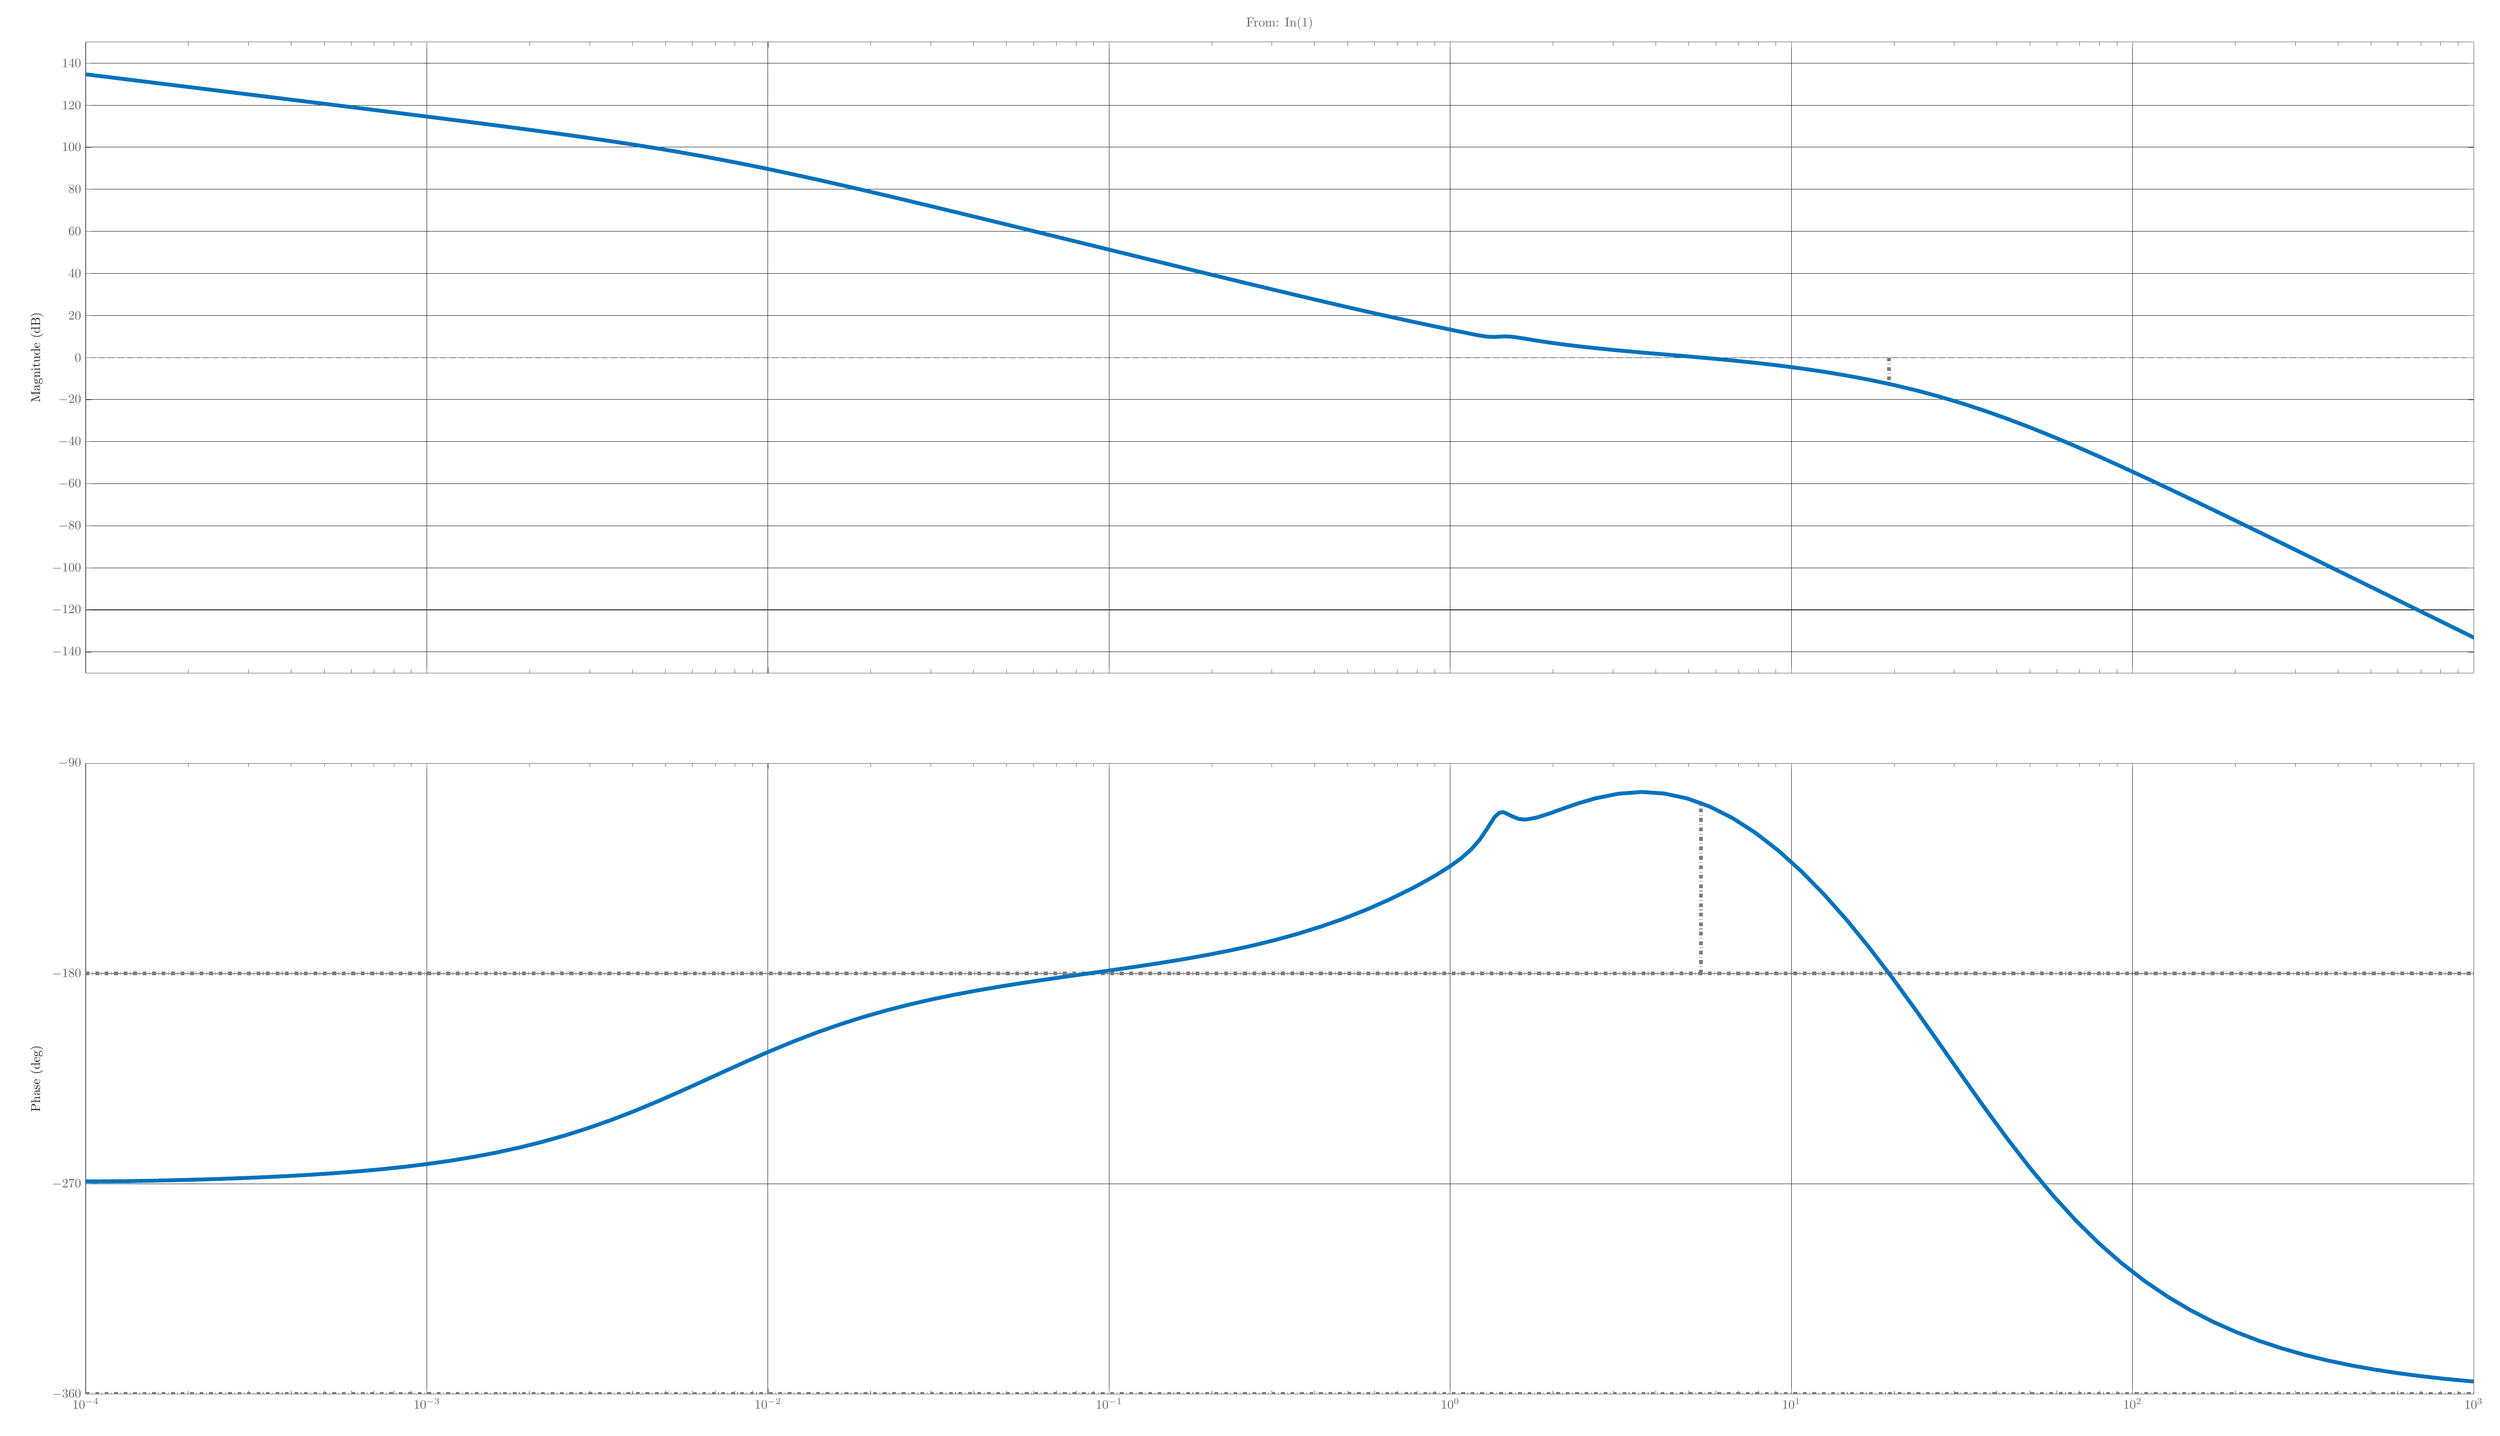
\begin{tikzpicture}

\begin{axis}[%
width=25.775in,
height=6.812in,
at={(0.787in,0.309in)},
scale only axis,
unbounded coords=jump,
separate axis lines,
every outer x axis line/.append style={mycolor3},
every x tick label/.append style={font=\color{mycolor3}},
every x tick/.append style={mycolor3},
xmode=log,
xmin=0.0001,
xmax=1000,
xminorticks=true,
every outer y axis line/.append style={mycolor3},
every y tick label/.append style={font=\color{mycolor3}},
every y tick/.append style={mycolor3},
ymin=-360,
ymax=-90,
ytick={-360, -270, -180,  -90},
ylabel style={font=\color{mycolor4}},
ylabel={Phase (deg)},
axis background/.style={fill=white},
xmajorgrids,
ymajorgrids,
grid style={mycolor4}
]
\addplot [color=mycolor1, line width=1.5pt, forget plot]
  table[row sep=crcr]{%
nan	-360\\
nan	-90\\
};
\addplot [color=mycolor1, line width=1.5pt, forget plot]
  table[row sep=crcr]{%
nan	-360\\
nan	-90\\
};
\addplot [color=mycolor1, dashdotted, line width=3.0pt, forget plot]
  table[row sep=crcr]{%
0.0001	-180\\
1000	-180\\
nan	nan\\
0.0001	-360\\
1000	-360\\
nan	nan\\
};
\addplot [color=mycolor1, dashdotted, line width=3.0pt, forget plot]
  table[row sep=crcr]{%
5.42949841575391	-180\\
5.42949841575391	-107.020038070252\\
nan	nan\\
};
\addplot [color=mycolor2, line width=3.0pt, forget plot]
  table[row sep=crcr]{%
-1e+20	-360\\
-1.75000000000006e+18	-360\\
-17500000000000.5	-359.999999999692\\
-1750000000.00005	-359.999996922034\\
-1750000.00000005	-359.9969220336\\
-17500.0000000005	-359.692203670225\\
-1750.00000000005	-356.922343794628\\
-1499.51714660699	-356.408375908165\\
-1284.8866702676	-355.808630817512\\
-1100.97691057884	-355.108825563096\\
-943.390717389322	-354.292318080901\\
-808.360318100068	-353.339728849051\\
-692.657232930111	-352.228508534768\\
-593.515084285727	-350.932447971935\\
-508.563454660752	-349.421129255444\\
-435.771211657978	-347.659321316114\\
-373.397945073613	-345.606331291816\\
-319.952354940388	-343.215336203711\\
-274.156595617363	-340.432740571937\\
-234.915723419213	-337.197638345075\\
-201.291517299819	-333.441506500702\\
-172.48004666149	-329.088327824387\\
-147.792449952269	-324.05543489486\\
-126.638464481415	-318.255483025876\\
-108.512313662775	-311.600078367888\\
-92.9806142601842	-304.005660631851\\
-79.6720145058243	-295.402174280758\\
-68.2683153464004	-285.74471304745\\
-58.4968625325129	-275.027531559982\\
-50.12402765155	-263.298530330857\\
-42.9496222402856	-250.670791250168\\
-36.8021114226282	-237.326704214182\\
-31.5345126340402	-223.510748427686\\
-27.0208813740781	-209.509782813283\\
-23.1532999639213	-195.624170440597\\
-19.839297312248	-182.137094112412\\
-16.9996379979137	-169.290570549487\\
-14.56642780799	-157.274075346492\\
-12.481490435939	-146.226813859356\\
-10.6949765279435	-136.250071147949\\
-9.16417182069149	-127.423532511336\\
-7.85247587404519	-119.819299902326\\
-6.7285269808275	-113.508973043374\\
-5.76545233094759	-108.561866483658\\
-4.94022550182908	-105.035352565596\\
-4.23311591319864	-102.960448412046\\
-3.65537477663796	-102.32454484816\\
-3.6272170830949	-102.326277293982\\
-3.10804240603796	-103.065637080323\\
-2.66317878870596	-105.039861215203\\
-2.39237635077625	-107.015608647208\\
-2.14399148550879	-109.397305851084\\
-1.95196026166226	-111.538657944906\\
-1.80130128659818	-113.177340519737\\
-1.68160667044661	-114.034278392502\\
-1.64845285105767	-114.093307704997\\
-1.58548448116874	-113.81840123128\\
-1.50757886072228	-112.526639439479\\
-1.44393831174424	-111.135285293291\\
-1.41957163236147	-110.941268701905\\
-1.39159923312488	-111.264874367195\\
-1.35500109262074	-112.755630213267\\
-1.34115731252706	-113.603632838799\\
-1.28454204027905	-117.897951557933\\
-1.22142376581715	-122.640843413019\\
-1.15160605608174	-126.918366951544\\
-1.07508301917166	-130.742619532461\\
-0.992104431462468	-134.394261625374\\
-0.903244457229831	-138.106456003623\\
-0.809466464172921	-142.017122482169\\
-0.773940231521999	-143.521422319161\\
-0.663163798637822	-148.342312279952\\
-0.56824313546652	-152.662727736184\\
-0.486908757184994	-156.52171449139\\
-0.417216017275415	-159.953595584924\\
-0.357498612424882	-162.996707386722\\
-0.30632874241103	-165.69304649832\\
-0.262482972425075	-168.086214016479\\
-0.224912981625005	-170.219583461767\\
-0.192720498537822	-172.135099195387\\
-0.165135824034344	-173.872667609202\\
-0.141499428376324	-175.469996408779\\
-0.121246182334502	-176.962738662178\\
-0.103891845354982	-178.38482856349\\
-0.0890214877156756	-179.768927234281\\
-0.0762795698549229	-181.146920590872\\
-0.0653614416761481	-182.550425413864\\
-0.0560060585830479	-184.011264324024\\
-0.0479897400909448	-185.561865545687\\
-0.0411208217871901	-187.235528804491\\
-0.0352350727728342	-189.066473885323\\
-0.0301917690198906	-191.089553474917\\
-0.0258703287609841	-193.339470204048\\
-0.022167429465974	-195.849299759223\\
-0.0189945374745303	-198.64811132683\\
-0.016275791219958	-201.757536534607\\
-0.0139461874336696	-205.187329405494\\
-0.011950026963761	-208.930337618363\\
-0.0102395830483286	-212.957855919845\\
-0.00877396020289974	-217.216881811637\\
-0.00751811643879721	-221.630967007947\\
-0.0064420254343794	-226.105736074599\\
-0.00551995862727427	-230.538655030218\\
-0.00472987006294783	-234.830884958209\\
-0.00405286929177894	-238.89809468552\\
-0.00347276971198815	-242.677590481836\\
-0.00297570155962486	-246.130712043948\\
-0.00254978029248143	-249.241127409941\\
-0.00218482243923222	-252.010607869552\\
-0.00187210211995447	-254.453928936796\\
-0.00160414241661196	-256.59407456701\\
-0.00137453660531951	-258.458340961802\\
-0.00117779497618029	-260.075490044592\\
-0.00100921357826849	-261.473850407737\\
-0.000864761751544091	-262.680164980302\\
-0.000740985756668697	-263.718976629895\\
-0.000634926198580705	-264.612375268438\\
-0.000544047269486704	-265.379972970933\\
-0.000466176119520002	-266.039013074496\\
-0.000399450905462247	-266.604550441536\\
-0.000342276275410462	-267.089662782865\\
-0.000293285225059857	-267.505668581788\\
-0.000251306413613561	-267.862337514832\\
-0.00021533615786619	-268.168085894962\\
-0.000184514434859893	-268.430153776639\\
-0.000158104319353657	-268.654762825299\\
-0.000135474364470531	-268.847255460969\\
-1.35474364470531e-05	-269.884710423675\\
-1.35474364470531e-07	-269.998847102709\\
-1.35474364470531e-10	-269.999998847103\\
-1.35474364470531e-14	-269.999999999885\\
-1.3547436447053e-19	-270\\
-1e-20	-270\\
1e-20	-270\\
1.3547436447053e-19	-270\\
1.35474364470531e-14	-269.999999999885\\
1.35474364470531e-10	-269.999998847103\\
1.35474364470531e-07	-269.998847102709\\
1.35474364470531e-05	-269.884710423675\\
0.000135474364470531	-268.847255460969\\
0.000158104319353657	-268.654762825299\\
0.000184514434859893	-268.430153776639\\
0.00021533615786619	-268.168085894962\\
0.000251306413613561	-267.862337514832\\
0.000293285225059857	-267.505668581788\\
0.000342276275410462	-267.089662782865\\
0.000399450905462247	-266.604550441536\\
0.000466176119520002	-266.039013074496\\
0.000544047269486704	-265.379972970933\\
0.000634926198580705	-264.612375268438\\
0.000740985756668697	-263.718976629895\\
0.000864761751544091	-262.680164980302\\
0.00100921357826849	-261.473850407737\\
0.00117779497618029	-260.075490044592\\
0.00137453660531951	-258.458340961802\\
0.00160414241661196	-256.59407456701\\
0.00187210211995447	-254.453928936796\\
0.00218482243923222	-252.010607869552\\
0.00254978029248143	-249.241127409941\\
0.00297570155962486	-246.130712043948\\
0.00347276971198815	-242.677590481836\\
0.00405286929177894	-238.89809468552\\
0.00472987006294783	-234.830884958209\\
0.00551995862727427	-230.538655030218\\
0.0064420254343794	-226.105736074599\\
0.00751811643879721	-221.630967007947\\
0.00877396020289974	-217.216881811637\\
0.0102395830483286	-212.957855919845\\
0.011950026963761	-208.930337618363\\
0.0139461874336696	-205.187329405494\\
0.016275791219958	-201.757536534607\\
0.0189945374745303	-198.64811132683\\
0.022167429465974	-195.849299759223\\
0.0258703287609841	-193.339470204048\\
0.0301917690198906	-191.089553474917\\
0.0352350727728342	-189.066473885323\\
0.0411208217871901	-187.235528804491\\
0.0479897400909448	-185.561865545687\\
0.0560060585830479	-184.011264324024\\
0.0653614416761481	-182.550425413864\\
0.0762795698549229	-181.146920590872\\
0.0890214877156756	-179.768927234281\\
0.103891845354982	-178.38482856349\\
0.121246182334502	-176.962738662178\\
0.141499428376324	-175.469996408779\\
0.165135824034344	-173.872667609202\\
0.192720498537822	-172.135099195387\\
0.224912981625005	-170.219583461767\\
0.262482972425075	-168.086214016479\\
0.30632874241103	-165.69304649832\\
0.357498612424882	-162.996707386722\\
0.417216017275415	-159.953595584924\\
0.486908757184994	-156.52171449139\\
0.56824313546652	-152.662727736184\\
0.663163798637822	-148.342312279952\\
0.773940231521999	-143.521422319161\\
0.809466464172921	-142.017122482169\\
0.903244457229831	-138.106456003623\\
0.992104431462468	-134.394261625374\\
1.07508301917166	-130.742619532461\\
1.15160605608174	-126.918366951544\\
1.22142376581715	-122.640843413019\\
1.28454204027905	-117.897951557933\\
1.34115731252706	-113.603632838799\\
1.35500109262074	-112.755630213267\\
1.39159923312488	-111.264874367195\\
1.41957163236147	-110.941268701905\\
1.44393831174424	-111.135285293291\\
1.50757886072228	-112.526639439479\\
1.58548448116874	-113.81840123128\\
1.64845285105767	-114.093307704997\\
1.68160667044661	-114.034278392502\\
1.80130128659818	-113.177340519737\\
1.95196026166226	-111.538657944906\\
2.14399148550879	-109.397305851084\\
2.39237635077625	-107.015608647208\\
2.66317878870596	-105.039861215203\\
3.10804240603796	-103.065637080323\\
3.6272170830949	-102.326277293982\\
3.65537477663796	-102.32454484816\\
4.23311591319864	-102.960448412046\\
4.94022550182908	-105.035352565596\\
5.76545233094759	-108.561866483658\\
6.7285269808275	-113.508973043374\\
7.85247587404519	-119.819299902326\\
9.16417182069149	-127.423532511336\\
10.6949765279435	-136.250071147949\\
12.481490435939	-146.226813859356\\
14.56642780799	-157.274075346492\\
16.9996379979137	-169.290570549487\\
19.839297312248	-182.137094112412\\
23.1532999639213	-195.624170440597\\
27.0208813740781	-209.509782813283\\
31.5345126340402	-223.510748427686\\
36.8021114226282	-237.326704214182\\
42.9496222402856	-250.670791250168\\
50.12402765155	-263.298530330857\\
58.4968625325129	-275.027531559982\\
68.2683153464004	-285.74471304745\\
79.6720145058243	-295.402174280758\\
92.9806142601842	-304.005660631851\\
108.512313662775	-311.600078367888\\
126.638464481415	-318.255483025876\\
147.792449952269	-324.05543489486\\
172.48004666149	-329.088327824387\\
201.291517299819	-333.441506500702\\
234.915723419213	-337.197638345075\\
274.156595617363	-340.432740571937\\
319.952354940388	-343.215336203711\\
373.397945073613	-345.606331291816\\
435.771211657978	-347.659321316114\\
508.563454660752	-349.421129255444\\
593.515084285727	-350.932447971935\\
692.657232930111	-352.228508534768\\
808.360318100068	-353.339728849051\\
943.390717389322	-354.292318080901\\
1100.97691057884	-355.108825563096\\
1284.8866702676	-355.808630817512\\
1499.51714660699	-356.408375908165\\
1750.00000000005	-356.922343794628\\
17500.0000000005	-359.692203670225\\
1750000.00000005	-359.9969220336\\
1750000000.00005	-359.999996922034\\
17500000000000.5	-359.999999999692\\
1.75000000000006e+18	-360\\
1e+20	-360\\
};
\addplot[only marks, mark=*, mark options={}, mark size=1.5000pt, draw=mycolor2, fill=white, forget plot] table[row sep=crcr]{%
x	y\\
nan	nan\\
};
\addplot[only marks, mark=*, mark options={}, mark size=1.5000pt, draw=mycolor2, fill=mycolor2, forget plot] table[row sep=crcr]{%
x	y\\
5.42949841575391	-107.191262509792\\
};
\end{axis}

\begin{axis}[%
width=25.775in,
height=6.812in,
at={(0.787in,8.095in)},
scale only axis,
unbounded coords=jump,
separate axis lines,
every outer x axis line/.append style={mycolor3},
every x tick label/.append style={font=\color{mycolor3}},
every x tick/.append style={mycolor3},
xmode=log,
xmin=0.0001,
xmax=1000,
xtick={0.0001,0.001,0.01,0.1,1,10,100,1000},
xticklabels={\empty},
xminorticks=true,
every outer y axis line/.append style={mycolor3},
every y tick label/.append style={font=\color{mycolor3}},
every y tick/.append style={mycolor3},
ymin=-150,
ymax=150,
ylabel style={font=\color{mycolor4}},
ylabel={Magnitude (dB)},
axis background/.style={fill=white},
title style={font=\color{mycolor3}},
title={From: In(1)},
xmajorgrids,
ymajorgrids,
grid style={mycolor4}
]
\addplot [color=mycolor1, line width=1.5pt, forget plot]
  table[row sep=crcr]{%
nan	-150\\
nan	150\\
};
\addplot [color=mycolor1, line width=1.5pt, forget plot]
  table[row sep=crcr]{%
nan	-150\\
nan	150\\
};
\addplot [color=mycolor1, dashdotted, forget plot]
  table[row sep=crcr]{%
0.0001	0\\
1000	0\\
};
\addplot [color=mycolor1, dashdotted, line width=3.0pt, forget plot]
  table[row sep=crcr]{%
19.3456508044871	0\\
19.3456508044871	-12.5654903989516\\
nan	nan\\
};
\addplot [color=mycolor2, line width=3.0pt, forget plot]
  table[row sep=crcr]{%
-1e+20	-1493.11305616064\\
-1.75000000000006e+18	-1352.55610005555\\
-17500000000000.5	-952.556100055548\\
-1750000000.00005	-632.556100055548\\
-1750000.00000005	-392.556100059561\\
-17500.0000000005	-232.556140193121\\
-1750.00000000005	-152.560113186805\\
-1499.51714660699	-147.194636578772\\
-1284.8866702676	-141.829685452934\\
-1100.97691057884	-136.46544979986\\
-943.390717389322	-131.102188190061\\
-808.360318100068	-125.740252433322\\
-692.657232930111	-120.380121023292\\
-593.515084285727	-115.022444427686\\
-508.563454660752	-109.6681062913\\
-435.771211657978	-104.318305905918\\
-373.397945073613	-98.9746689007016\\
-319.952354940388	-93.6393950084474\\
-274.156595617363	-88.3154538592203\\
-234.915723419213	-83.006841737587\\
-201.291517299819	-77.7189134414492\\
-172.48004666149	-72.4588025000843\\
-147.792449952269	-67.2359377646133\\
-126.638464481415	-62.0626511465255\\
-108.512313662775	-56.9548449949225\\
-92.9806142601842	-51.9326427062692\\
-79.6720145058243	-47.0208797410563\\
-68.2683153464004	-42.2492108798124\\
-58.4968625325129	-37.6515397599287\\
-50.12402765155	-33.2644729581905\\
-42.9496222402856	-29.1246364866206\\
-36.8021114226282	-25.2650152723761\\
-31.5345126340402	-21.7109325121174\\
-27.0208813740781	-18.4766732981301\\
-23.1532999639213	-15.5637964267767\\
-19.839297312248	-12.9617196918996\\
-16.9996379979137	-10.6503666515255\\
-14.56642780799	-8.60393622705645\\
-12.481490435939	-6.79456549335171\\
-10.6949765279435	-5.19487136787905\\
-9.16417182069149	-3.77887971292539\\
-7.85247587404519	-2.52142106981775\\
-6.7285269808275	-1.39651749521739\\
-5.76545233094759	-0.375515661671108\\
-4.94022550182908	0.574307889832187\\
-4.23311591319864	1.49021501446757\\
-3.65537477663796	2.36643161056958\\
-3.6272170830949	2.41350133724519\\
-3.10804240603796	3.38840252741309\\
-2.66317878870596	4.46130725521163\\
-2.39237635077625	5.28982932812777\\
-2.14399148550879	6.23041466916585\\
-1.95196026166226	7.13024008834051\\
-1.80130128659818	7.98537662523051\\
-1.68160667044661	8.78076029776561\\
-1.64845285105767	9.01702522094903\\
-1.58548448116874	9.46654727042516\\
-1.50757886072228	9.92827871747167\\
-1.44393831174424	10.0459791066089\\
-1.41957163236147	10.0011993725895\\
-1.39159923312488	9.90921404259926\\
-1.35500109262074	9.79746666199222\\
-1.34115731252706	9.77853452096572\\
-1.28454204027905	9.91821274746286\\
-1.22142376581715	10.4332070343182\\
-1.15160605608174	11.2305143760277\\
-1.07508301917166	12.2244470342025\\
-0.992104431462468	13.397483878872\\
-0.903244457229831	14.7755370707826\\
-0.809466464172921	16.4064035010969\\
-0.773940231521999	17.0827504811094\\
-0.663163798637822	19.4528241701571\\
-0.56824313546652	21.8863897294388\\
-0.486908757184994	24.375502071441\\
-0.417216017275415	26.9102075188821\\
-0.357498612424882	29.4810012124926\\
-0.30632874241103	32.079692214114\\
-0.262482972425075	34.6995817386554\\
-0.224912981625005	37.3353523679453\\
-0.192720498537822	39.9828523465005\\
-0.165135824034344	42.6388598712172\\
-0.141499428376324	45.3008634388229\\
-0.121246182334502	47.9668699833867\\
-0.103891845354982	50.6352407454833\\
-0.0890214877156756	53.3045494445297\\
-0.0762795698549229	55.9734551227156\\
-0.0653614416761481	58.6405812781046\\
-0.0560060585830479	61.3043927669005\\
-0.0479897400909448	63.9630621337723\\
-0.0411208217871901	66.6143176319447\\
-0.0352350727728342	69.255266725903\\
-0.0301917690198906	71.8821923077501\\
-0.0258703287609841	74.4903257449308\\
-0.022167429465974	77.0736132491221\\
-0.0189945374745303	79.6245118724789\\
-0.016275791219958	82.1338789250159\\
-0.0139461874336696	84.591048985227\\
-0.011950026963761	86.9842117722853\\
-0.0102395830483286	89.3011864535216\\
-0.00877396020289974	91.5306049138257\\
-0.00751811643879721	93.6633619442408\\
-0.0064420254343794	95.6940134136179\\
-0.00551995862727427	97.6217111589519\\
-0.00472987006294783	99.4503544332675\\
-0.00405286929177894	101.187902889447\\
-0.00347276971198815	102.845093179918\\
-0.00297570155962486	104.433961974994\\
-0.00254978029248143	105.966542437858\\
-0.00218482243923222	107.453940022322\\
-0.00187210211995447	108.905821952583\\
-0.00160414241661196	110.330245099721\\
-0.00137453660531951	111.733709150066\\
-0.00117779497618029	113.121331474255\\
-0.00100921357826849	114.497068618146\\
-0.000864761751544091	115.863938594972\\
-0.000740985756668697	117.224220573204\\
-0.000634926198580705	118.579623045199\\
-0.000544047269486704	119.931419726191\\
-0.000466176119520002	121.280556370527\\
-0.000399450905462247	122.627733130849\\
-0.000342276275410462	123.973467204659\\
-0.000293285225059857	125.318140027182\\
-0.000251306413613561	126.662032575586\\
-0.00021533615786619	128.005351646466\\
-0.000184514434859893	129.348249342929\\
-0.000158104319353657	130.69083748738\\
-0.000135474364470531	132.033198260499\\
-1.35474364470531e-05	152.034917671559\\
-1.35474364470531e-07	192.034935041084\\
-1.35474364470531e-10	252.034935042821\\
-1.35474364470531e-14	332.034935042821\\
-1.3547436447053e-19	432.034935042821\\
-1e-20	454.672077489864\\
1e-20	454.672077489864\\
1.3547436447053e-19	432.034935042821\\
1.35474364470531e-14	332.034935042821\\
1.35474364470531e-10	252.034935042821\\
1.35474364470531e-07	192.034935041084\\
1.35474364470531e-05	152.034917671559\\
0.000135474364470531	132.033198260499\\
0.000158104319353657	130.69083748738\\
0.000184514434859893	129.348249342929\\
0.00021533615786619	128.005351646466\\
0.000251306413613561	126.662032575586\\
0.000293285225059857	125.318140027182\\
0.000342276275410462	123.973467204659\\
0.000399450905462247	122.627733130849\\
0.000466176119520002	121.280556370527\\
0.000544047269486704	119.931419726191\\
0.000634926198580705	118.579623045199\\
0.000740985756668697	117.224220573204\\
0.000864761751544091	115.863938594972\\
0.00100921357826849	114.497068618146\\
0.00117779497618029	113.121331474255\\
0.00137453660531951	111.733709150066\\
0.00160414241661196	110.330245099721\\
0.00187210211995447	108.905821952583\\
0.00218482243923222	107.453940022322\\
0.00254978029248143	105.966542437858\\
0.00297570155962486	104.433961974994\\
0.00347276971198815	102.845093179918\\
0.00405286929177894	101.187902889447\\
0.00472987006294783	99.4503544332675\\
0.00551995862727427	97.6217111589519\\
0.0064420254343794	95.6940134136179\\
0.00751811643879721	93.6633619442408\\
0.00877396020289974	91.5306049138257\\
0.0102395830483286	89.3011864535216\\
0.011950026963761	86.9842117722853\\
0.0139461874336696	84.591048985227\\
0.016275791219958	82.1338789250159\\
0.0189945374745303	79.6245118724789\\
0.022167429465974	77.0736132491221\\
0.0258703287609841	74.4903257449308\\
0.0301917690198906	71.8821923077501\\
0.0352350727728342	69.255266725903\\
0.0411208217871901	66.6143176319447\\
0.0479897400909448	63.9630621337723\\
0.0560060585830479	61.3043927669005\\
0.0653614416761481	58.6405812781046\\
0.0762795698549229	55.9734551227156\\
0.0890214877156756	53.3045494445297\\
0.103891845354982	50.6352407454833\\
0.121246182334502	47.9668699833867\\
0.141499428376324	45.3008634388229\\
0.165135824034344	42.6388598712172\\
0.192720498537822	39.9828523465005\\
0.224912981625005	37.3353523679453\\
0.262482972425075	34.6995817386554\\
0.30632874241103	32.079692214114\\
0.357498612424882	29.4810012124926\\
0.417216017275415	26.9102075188821\\
0.486908757184994	24.375502071441\\
0.56824313546652	21.8863897294388\\
0.663163798637822	19.4528241701571\\
0.773940231521999	17.0827504811094\\
0.809466464172921	16.4064035010969\\
0.903244457229831	14.7755370707826\\
0.992104431462468	13.397483878872\\
1.07508301917166	12.2244470342025\\
1.15160605608174	11.2305143760277\\
1.22142376581715	10.4332070343182\\
1.28454204027905	9.91821274746286\\
1.34115731252706	9.77853452096572\\
1.35500109262074	9.79746666199222\\
1.39159923312488	9.90921404259926\\
1.41957163236147	10.0011993725895\\
1.44393831174424	10.0459791066089\\
1.50757886072228	9.92827871747167\\
1.58548448116874	9.46654727042516\\
1.64845285105767	9.01702522094903\\
1.68160667044661	8.78076029776561\\
1.80130128659818	7.98537662523051\\
1.95196026166226	7.13024008834051\\
2.14399148550879	6.23041466916585\\
2.39237635077625	5.28982932812777\\
2.66317878870596	4.46130725521163\\
3.10804240603796	3.38840252741309\\
3.6272170830949	2.41350133724519\\
3.65537477663796	2.36643161056958\\
4.23311591319864	1.49021501446757\\
4.94022550182908	0.574307889832187\\
5.76545233094759	-0.375515661671108\\
6.7285269808275	-1.39651749521739\\
7.85247587404519	-2.52142106981775\\
9.16417182069149	-3.77887971292539\\
10.6949765279435	-5.19487136787905\\
12.481490435939	-6.79456549335171\\
14.56642780799	-8.60393622705645\\
16.9996379979137	-10.6503666515255\\
19.839297312248	-12.9617196918996\\
23.1532999639213	-15.5637964267767\\
27.0208813740781	-18.4766732981301\\
31.5345126340402	-21.7109325121174\\
36.8021114226282	-25.2650152723761\\
42.9496222402856	-29.1246364866206\\
50.12402765155	-33.2644729581905\\
58.4968625325129	-37.6515397599287\\
68.2683153464004	-42.2492108798124\\
79.6720145058243	-47.0208797410563\\
92.9806142601842	-51.9326427062692\\
108.512313662775	-56.9548449949225\\
126.638464481415	-62.0626511465255\\
147.792449952269	-67.2359377646133\\
172.48004666149	-72.4588025000843\\
201.291517299819	-77.7189134414492\\
234.915723419213	-83.006841737587\\
274.156595617363	-88.3154538592203\\
319.952354940388	-93.6393950084474\\
373.397945073613	-98.9746689007016\\
435.771211657978	-104.318305905918\\
508.563454660752	-109.6681062913\\
593.515084285727	-115.022444427686\\
692.657232930111	-120.380121023292\\
808.360318100068	-125.740252433322\\
943.390717389322	-131.102188190061\\
1100.97691057884	-136.46544979986\\
1284.8866702676	-141.829685452934\\
1499.51714660699	-147.194636578772\\
1750.00000000005	-152.560113186805\\
17500.0000000005	-232.556140193121\\
1750000.00000005	-392.556100059561\\
1750000000.00005	-632.556100055548\\
17500000000000.5	-952.556100055548\\
1.75000000000006e+18	-1352.55610005555\\
1e+20	-1493.11305616064\\
};
\addplot[only marks, mark=*, mark options={}, mark size=1.5000pt, draw=mycolor2, fill=white, forget plot] table[row sep=crcr]{%
x	y\\
nan	nan\\
};
\addplot[only marks, mark=*, mark options={}, mark size=1.5000pt, draw=mycolor2, fill=mycolor2, forget plot] table[row sep=crcr]{%
x	y\\
19.3456508044871	-12.5654903989516\\
};
\end{axis}

\begin{axis}[%
width=26.667in,
height=15in,
at={(0in,0in)},
scale only axis,
xmin=0,
xmax=1,
ymin=0,
ymax=1,
axis line style={draw=none},
ticks=none,
axis x line*=bottom,
axis y line*=left
]
\end{axis}
\end{tikzpicture}%}
\caption{Design C: Open-loop Bode plot showing crossover at 5.43~rad/s with phase margin of 73°. Lead compensation provides significant phase boost near crossover.}
\label{fig:design_C_bode}
\end{figure}

\paragraph{Linear Step Response.}
Figure~\ref{fig:design_C_step} shows the ideal linear response to a 30$^\circ$ command. The rise time is 0.24~s with zero overshoot, indicating critically damped response. The settling time (2\%) is 0.34~s with steady-state error less than 0.01\%.

\begin{figure}[h!]
\centering
\resizebox{0.7\textwidth}{!}{% This file was created by matlab2tikz.
%
\definecolor{mycolor1}{rgb}{0.49020,0.49020,0.49020}%
\definecolor{mycolor2}{rgb}{0.00000,0.44700,0.74100}%
\definecolor{mycolor3}{rgb}{0.38039,0.38039,0.38039}%
\definecolor{mycolor4}{rgb}{0.12941,0.12941,0.12941}%
%
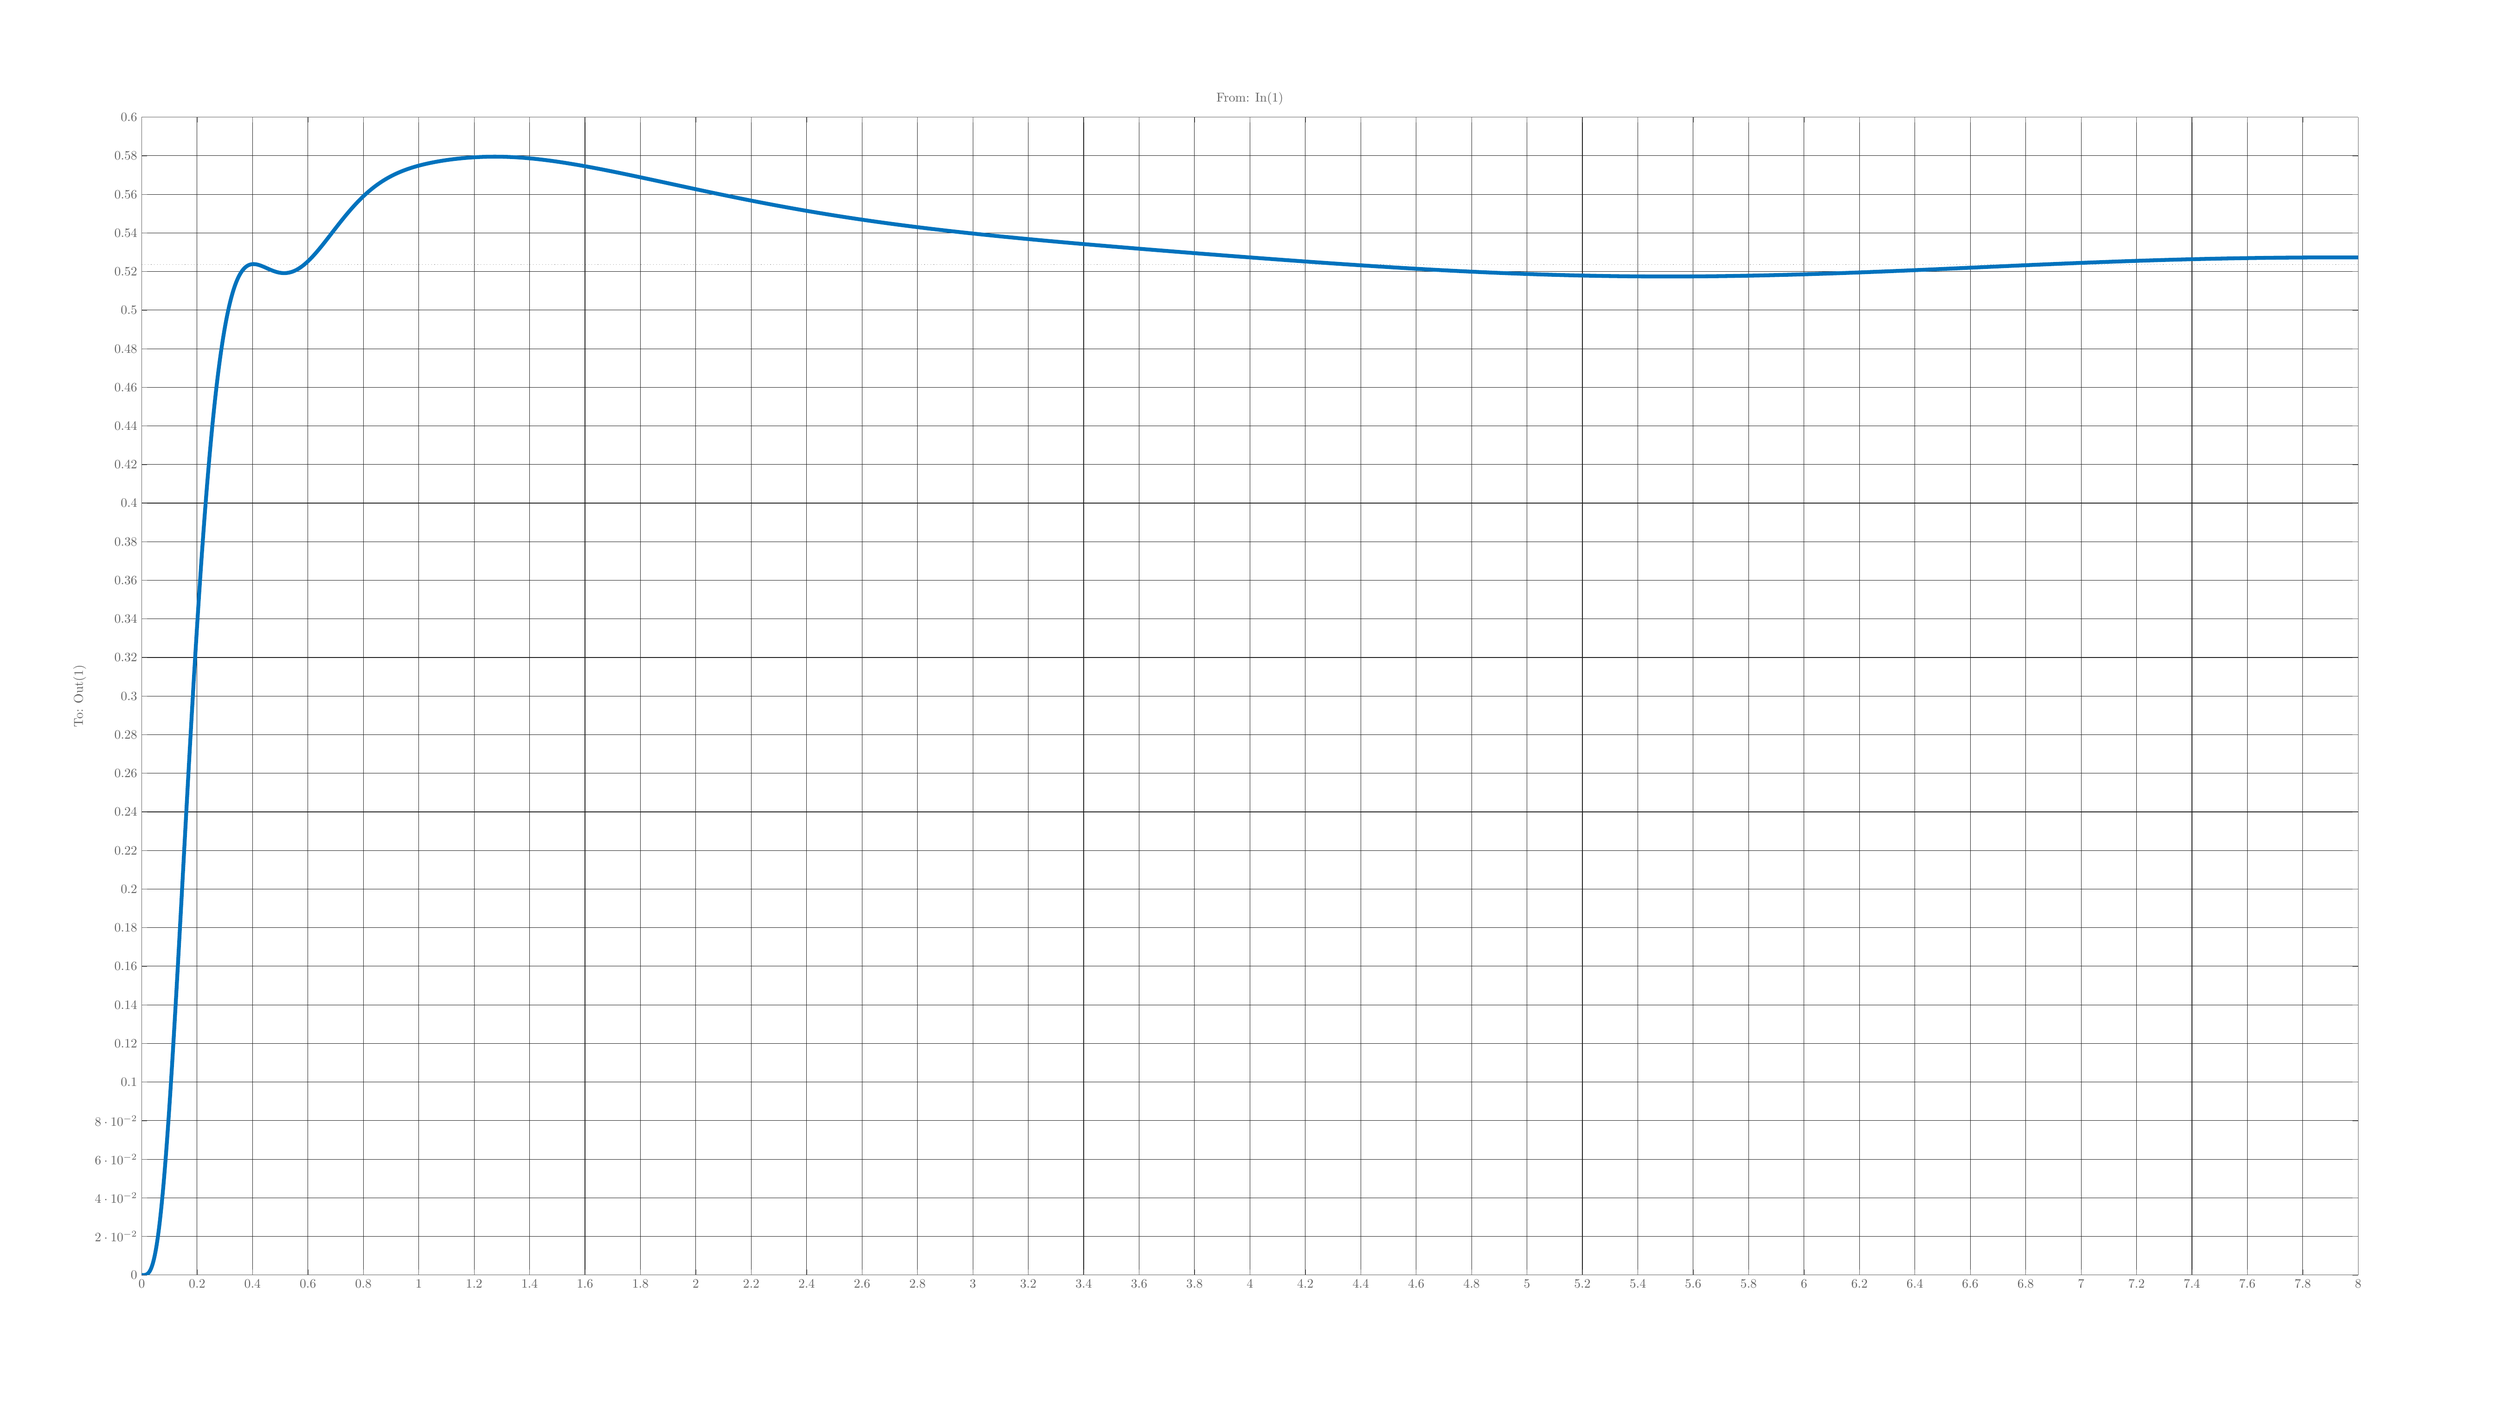
\begin{tikzpicture}

\begin{axis}[%
width=23.889in,
height=12.486in,
at={(1.389in,1.389in)},
scale only axis,
separate axis lines,
every outer x axis line/.append style={mycolor3},
every x tick label/.append style={font=\color{mycolor3}},
every x tick/.append style={mycolor3},
xmin=0,
xmax=8,
every outer y axis line/.append style={mycolor3},
every y tick label/.append style={font=\color{mycolor3}},
every y tick/.append style={mycolor3},
ymin=0,
ymax=0.6,
ylabel style={font=\color{mycolor3}},
ylabel={To: Out(1)},
axis background/.style={fill=white},
title style={font=\color{mycolor3}},
title={From: In(1)},
xmajorgrids,
ymajorgrids,
grid style={mycolor4}
]
\addplot [color=mycolor1, dotted, forget plot]
  table[row sep=crcr]{%
0	0.523598775598299\\
8	0.523598775598299\\
};
\addplot [color=mycolor2, line width=3.0pt, forget plot]
  table[row sep=crcr]{%
0	0\\
0.00224215246636771	1.16822125479921e-07\\
0.00448430493273543	1.79247314274625e-06\\
0.00672645739910314	8.70368356406195e-06\\
0.00896860986547085	2.63889099866725e-05\\
0.0112107623318386	6.18163093030744e-05\\
0.0134529147982063	0.000123012115304548\\
0.015695067264574	0.000218742516642965\\
0.0179372197309417	0.000358242833050481\\
0.0201793721973094	0.00055098842072789\\
0.0224215246636771	0.000806502313188657\\
0.0246636771300448	0.00113419512549149\\
0.0269058295964126	0.00154323322225225\\
0.0291479820627803	0.00204243157729849\\
0.031390134529148	0.0026401681392001\\
0.0336322869955157	0.003344316865762\\
0.0358744394618834	0.00416219690520411\\
0.0381165919282511	0.00510053568522361\\
0.0403587443946188	0.00616544392623555\\
0.0426008968609865	0.00736240082439372\\
0.0448430493273543	0.00869624785586757\\
0.047085201793722	0.0101711898384608\\
0.0493273542600897	0.0117908020519888\\
0.0515695067264574	0.0135580423667042\\
0.0538116591928251	0.0154752674611358\\
0.0560538116591928	0.0175442523285032\\
0.0582959641255605	0.0197662123757764\\
0.0605381165919283	0.0221418275127343\\
0.062780269058296	0.0246712677111779\\
0.0650224215246637	0.0273542195878414\\
0.0672645739910314	0.0301899136294517\\
0.0695067264573991	0.0331771517356901\\
0.0717488789237668	0.0363143348062973\\
0.0739910313901345	0.0395994901429343\\
0.0762331838565022	0.0430302984753297\\
0.07847533632287	0.0466041204552746\\
0.0807174887892377	0.0503180224917145\\
0.0829596412556054	0.0541688018259913\\
0.0852017937219731	0.0581530107686556\\
0.0874439461883408	0.0622669800385724\\
0.0896860986547085	0.0665068411616392\\
0.0919282511210762	0.070868547900631\\
0.0941704035874439	0.0753478966997712\\
0.0964125560538117	0.0799405461378415\\
0.0986547085201794	0.0846420353922235\\
0.100896860986547	0.0894478017234064\\
0.103139013452915	0.0943531969953782\\
0.105381165919283	0.0993535032521093\\
0.10762331838565	0.104443947374169\\
0.109865470852018	0.109619714842527\\
0.112107623318386	0.114875962638892\\
0.114349775784753	0.120207831313613\\
0.116591928251121	0.125610456253345\\
0.118834080717489	0.131078978181379\\
0.121076233183857	0.136608552923869\\
0.123318385650224	0.142194360475237\\
0.125560538116592	0.14783161339575\\
0.12780269058296	0.153515564573825\\
0.130044843049327	0.15924151438498\\
0.132286995515695	0.165004817278549\\
0.134529147982063	0.1708008878224\\
0.13677130044843	0.176625206234908\\
0.139013452914798	0.18247332343239\\
0.141255605381166	0.188340865619135\\
0.143497757847534	0.194223538446027\\
0.145739910313901	0.200117130762657\\
0.147982062780269	0.206017517986669\\
0.150224215246637	0.211920665112979\\
0.152466367713004	0.217822629384401\\
0.154708520179372	0.223719562644114\\
0.15695067264574	0.229607713389377\\
0.159192825112108	0.235483428544861\\
0.161434977578475	0.24134315497297\\
0.163677130044843	0.247183440737596\\
0.165919282511211	0.253000936136824\\
0.168161434977578	0.258792394519235\\
0.170403587443946	0.264554672897621\\
0.172645739910314	0.270284732373149\\
0.174887892376682	0.275979638382232\\
0.177130044843049	0.281636560777677\\
0.179372197309417	0.287252773754995\\
0.181614349775785	0.292825655634124\\
0.183856502242152	0.298352688506213\\
0.18609865470852	0.303831457754544\\
0.188340807174888	0.30925965145816\\
0.190582959641256	0.314635059686227\\
0.192825112107623	0.319955573690734\\
0.195067264573991	0.325219185004648\\
0.197309417040359	0.330423984452274\\
0.199551569506726	0.335568161078137\\
0.201793721973094	0.340650001000378\\
0.204035874439462	0.345667886194297\\
0.20627802690583	0.35062029321136\\
0.208520179372197	0.355505791838692\\
0.210762331838565	0.360323043703809\\
0.213004484304933	0.365070800829058\\
0.2152466367713	0.369747904140019\\
0.217488789237668	0.374353281931873\\
0.219730941704036	0.378885948297546\\
0.221973094170404	0.383345001521213\\
0.224215246636771	0.387729622440594\\
0.226457399103139	0.392039072781261\\
0.228699551569507	0.396272693466047\\
0.230941704035874	0.400429902902462\\
0.233183856502242	0.404510195250895\\
0.23542600896861	0.408513138676243\\
0.237668161434978	0.412438373585473\\
0.239910313901345	0.416285610853498\\
0.242152466367713	0.420054630039656\\
0.244394618834081	0.423745277596944\\
0.246636771300448	0.427357465076076\\
0.248878923766816	0.430891167326335\\
0.251121076233184	0.434346420695089\\
0.253363228699552	0.437723321227759\\
0.255605381165919	0.441022022869958\\
0.257847533632287	0.444242735673397\\
0.260089686098655	0.447385724007146\\
0.262331838565022	0.450451304775701\\
0.26457399103139	0.453439845645277\\
0.266816143497758	0.456351763279671\\
0.269058295964126	0.459187521586979\\
0.271300448430493	0.461947629978372\\
0.273542600896861	0.46463264164011\\
0.275784753363229	0.467243151819886\\
0.278026905829596	0.469779796128555\\
0.280269058295964	0.47224324885824\\
0.282511210762332	0.474634221317769\\
0.2847533632287	0.476953460186331\\
0.286995515695067	0.479201745886211\\
0.289237668161435	0.481379890975388\\
0.291479820627803	0.48348873856078\\
0.29372197309417	0.485529160732826\\
0.295964125560538	0.487502057022095\\
0.298206278026906	0.489408352878537\\
0.300448430493274	0.491248998173985\\
0.302690582959641	0.49302496572844\\
0.304932735426009	0.494737249860667\\
0.307174887892377	0.496386864963581\\
0.309417040358744	0.497974844104842\\
0.311659192825112	0.499502237653099\\
0.31390134529148	0.500970111930225\\
0.316143497757848	0.502379547889899\\
0.318385650224215	0.503731639822832\\
0.320627802690583	0.505027494088925\\
0.322869955156951	0.506268227876584\\
0.325112107623318	0.507454967989427\\
0.327354260089686	0.508588849660556\\
0.329596412556054	0.509671015394553\\
0.331838565022422	0.510702613837331\\
0.334080717488789	0.511684798673955\\
0.336322869955157	0.512618727554482\\
0.338565022421525	0.513505561047905\\
0.340807174887892	0.514346461624205\\
0.34304932735426	0.515142592664531\\
0.345291479820628	0.515895117499471\\
0.347533632286996	0.516605198475396\\
0.349775784753363	0.517273996048798\\
0.352017937219731	0.517902667908537\\
0.354260089686099	0.518492368125905\\
0.356502242152466	0.519044246332378\\
0.358744394618834	0.519559446924912\\
0.360986547085202	0.520039108298623\\
0.36322869955157	0.520484362106681\\
0.365470852017937	0.52089633254721\\
0.367713004484305	0.521276135676996\\
0.369955156950673	0.521624878751776\\
0.37219730941704	0.521943659592851\\
0.374439461883408	0.522233565979796\\
0.376681614349776	0.522495675068972\\
0.378923766816143	0.522731052837568\\
0.381165919282511	0.522940753552889\\
0.383408071748879	0.523125819266564\\
0.385650224215247	0.523287279333373\\
0.387892376681614	0.523426149954359\\
0.390134529147982	0.523543433743889\\
0.39237668161435	0.523640119320309\\
0.394618834080717	0.523717180919851\\
0.396860986547085	0.523775578033415\\
0.399103139013453	0.523816255065859\\
0.401345291479821	0.523840141017412\\
0.403587443946188	0.523848149186836\\
0.405829596412556	0.523841176895925\\
0.408071748878924	0.523820105234959\\
0.410313901345291	0.5237857988287\\
0.412556053811659	0.523739105622523\\
0.414798206278027	0.523680856688268\\
0.417040358744395	0.523611866049401\\
0.419282511210762	0.523532930525054\\
0.42152466367713	0.523444829592526\\
0.423766816143498	0.523348325267824\\
0.426008968609865	0.523244162003798\\
0.428251121076233	0.523133066605466\\
0.430493273542601	0.52301574816207\\
0.432735426008969	0.522892897995449\\
0.434977578475336	0.522765189624291\\
0.437219730941704	0.522633278743828\\
0.439461883408072	0.522497803220543\\
0.441704035874439	0.522359383101453\\
0.443946188340807	0.522218620637544\\
0.446188340807175	0.522076100320919\\
0.448430493273543	0.52193238893523\\
0.45067264573991	0.521788035618974\\
0.452914798206278	0.521643571941218\\
0.455156950672646	0.521499511989338\\
0.457399103139013	0.521356352468341\\
0.459641255605381	0.521214572811366\\
0.461883408071749	0.521074635300935\\
0.464125560538117	0.520936985200558\\
0.466367713004484	0.520802050896265\\
0.468609865470852	0.52067024404768\\
0.47085201793722	0.520541959748228\\
0.473094170403587	0.520417576694076\\
0.475336322869955	0.520297457361429\\
0.477578475336323	0.520181948191778\\
0.479820627802691	0.520071379784734\\
0.482062780269058	0.519966067098061\\
0.484304932735426	0.519866309654542\\
0.486547085201794	0.519772391755306\\
0.488789237668161	0.519684582699265\\
0.491031390134529	0.51960313700829\\
0.493273542600897	0.519528294657795\\
0.495515695067265	0.519460281312367\\
0.497757847533632	0.519399308566125\\
0.5	0.519345574187449\\
0.502242152466368	0.51929926236778\\
0.504484304932735	0.519260543974156\\
0.506726457399103	0.519229576805169\\
0.508968609865471	0.519206505850056\\
0.511210762331839	0.519191463550589\\
0.513452914798206	0.519184570065506\\
0.515695067264574	0.519185933537172\\
0.517937219730942	0.519195650360199\\
0.520179372197309	0.519213805451743\\
0.522421524663677	0.519240472523221\\
0.524663677130045	0.519275714353176\\
0.526905829596413	0.519319583061047\\
0.52914798206278	0.519372120381579\\
0.531390134529148	0.519433357939655\\
0.533632286995516	0.519503317525291\\
0.535874439461883	0.519582011368588\\
0.538116591928251	0.519669442414405\\
0.540358744394619	0.519765604596546\\
0.542600896860987	0.519870483111248\\
0.544843049327354	0.519984054689779\\
0.547085201793722	0.520106287869932\\
0.54932735426009	0.520237143266254\\
0.551569506726457	0.520376573838803\\
0.553811659192825	0.520524525160272\\
0.556053811659193	0.52068093568131\\
0.55829596412556	0.520845736993873\\
0.560538116591928	0.521018854092453\\
0.562780269058296	0.521200205633032\\
0.565022421524664	0.521389704189626\\
0.567264573991031	0.521587256508266\\
0.569506726457399	0.521792763758302\\
0.571748878923767	0.522006121780892\\
0.573991031390135	0.522227221334561\\
0.576233183856502	0.522455948337723\\
0.57847533632287	0.52269218410804\\
0.580717488789238	0.522935805598543\\
0.582959641255605	0.523186685630389\\
0.585201793721973	0.523444693122186\\
0.587443946188341	0.523709693315791\\
0.589686098654709	0.523981547998498\\
0.591928251121076	0.524260115721548\\
0.594170403587444	0.524545252014887\\
0.596412556053812	0.524836809598109\\
0.598654708520179	0.525134638587521\\
0.600896860986547	0.525438586699282\\
0.603139013452915	0.525748499448556\\
0.605381165919282	0.526064220344646\\
0.60762331838565	0.526385591082055\\
0.609865470852018	0.526712451727448\\
0.612107623318386	0.527044640902477\\
0.614349775784753	0.527381995962449\\
0.616591928251121	0.527724353170794\\
0.618834080717489	0.528071547869346\\
0.621076233183857	0.52842341464439\\
0.623318385650224	0.528779787488482\\
0.625560538116592	0.529140499958022\\
0.62780269058296	0.529505385326596\\
0.630044843049327	0.529874276734056\\
0.632286995515695	0.53024700733137\\
0.634529147982063	0.530623410421235\\
0.63677130044843	0.531003319594451\\
0.639013452914798	0.531386568862101\\
0.641255605381166	0.531772992783513\\
0.643497757847534	0.532162426590056\\
0.645739910313901	0.532554706304772\\
0.647982062780269	0.532949668857869\\
0.650224215246637	0.533347152198119\\
0.652466367713004	0.533746995400168\\
0.654708520179372	0.534149038767797\\
0.65695067264574	0.534553123933186\\
0.659192825112108	0.534959093952183\\
0.661434977578475	0.535366793395652\\
0.663677130044843	0.535776068436914\\
0.665919282511211	0.536186766935339\\
0.668161434977579	0.536598738516127\\
0.670403587443946	0.537011834646326\\
0.672645739910314	0.537425908707137\\
0.674887892376682	0.537840816062549\\
0.677130044843049	0.538256414124361\\
0.679372197309417	0.538672562413646\\
0.681614349775785	0.539089122618703\\
0.683856502242152	0.539505958649553\\
0.68609865470852	0.539922936689049\\
0.688340807174888	0.540339925240635\\
0.690582959641256	0.540756795172833\\
0.692825112107623	0.541173419760504\\
0.695067264573991	0.541589674722949\\
0.697309417040359	0.542005438258915\\
0.699551569506726	0.542420591078557\\
0.701793721973094	0.542835016432428\\
0.704035874439462	0.543248600137555\\
0.70627802690583	0.54366123060067\\
0.708520179372197	0.544072798838654\\
0.710762331838565	0.544483198496259\\
0.713004484304933	0.544892325861182\\
0.7152466367713	0.54530007987654\\
0.717488789237668	0.545706362150826\\
0.719730941704036	0.546111076965408\\
0.721973094170404	0.546514131279623\\
0.724215246636771	0.546915434733557\\
0.726457399103139	0.547314899648551\\
0.728699551569507	0.547712441025519\\
0.730941704035874	0.548107976541121\\
0.733183856502242	0.548501426541885\\
0.73542600896861	0.548892714036315\\
0.737668161434978	0.549281764685066\\
0.739910313901345	0.549668506789246\\
0.742152466367713	0.55005287127691\\
0.744394618834081	0.550434791687804\\
0.746636771300448	0.550814204156433\\
0.748878923766816	0.551191047393505\\
0.751121076233184	0.551565262665818\\
0.753363228699552	0.551936793774655\\
0.755605381165919	0.552305587032736\\
0.757847533632287	0.552671591239803\\
0.760089686098655	0.553034757656892\\
0.762331838565022	0.553395039979336\\
0.76457399103139	0.55375239430859\\
0.766816143497758	0.554106779122899\\
0.769058295964126	0.554458155246896\\
0.771300448430493	0.554806485820164\\
0.773542600896861	0.555151736264836\\
0.775784753363229	0.555493874252268\\
0.778026905829596	0.555832869668861\\
0.780269058295964	0.556168694581059\\
0.782511210762332	0.556501323199601\\
0.784753363228699	0.556830731843058\\
0.786995515695067	0.557156898900717\\
0.789237668161435	0.557479804794853\\
0.791479820627803	0.557799431942446\\
0.79372197309417	0.55811576471638\\
0.795964125560538	0.55842878940618\\
0.798206278026906	0.558738494178327\\
0.800448430493274	0.559044869036196\\
0.802690582959641	0.559347905779661\\
0.804932735426009	0.559647597964409\\
0.807174887892377	0.559943940861008\\
0.809417040358744	0.560236931413759\\
0.811659192825112	0.560526568199384\\
0.81390134529148	0.560812851385584\\
0.816143497757848	0.5610957826895\\
0.818385650224215	0.561375365336113\\
0.820627802690583	0.561651604016634\\
0.822869955156951	0.561924504846893\\
0.825112107623318	0.56219407532578\\
0.827354260089686	0.562460324293765\\
0.829596412556054	0.562723261891524\\
0.831838565022421	0.562982899518707\\
0.834080717488789	0.563239249792871\\
0.836322869955157	0.563492326508617\\
0.838565022421525	0.563742144596944\\
0.840807174887892	0.56398872008486\\
0.84304932735426	0.564232070055264\\
0.845291479820628	0.564472212607136\\
0.847533632286996	0.564709166816039\\
0.849775784753363	0.564942952694985\\
0.852017937219731	0.565173591155652\\
0.854260089686099	0.565401103970001\\
0.856502242152466	0.565625513732301\\
0.858744394618834	0.565846843821573\\
0.860986547085202	0.566065118364493\\
0.863228699551569	0.566280362198745\\
0.865470852017937	0.566492600836861\\
0.867713004484305	0.566701860430553\\
0.869955156950673	0.566908167735554\\
0.87219730941704	0.567111550076975\\
0.874439461883408	0.56731203531521\\
0.876681614349776	0.567509651812381\\
0.878923766816143	0.567704428399333\\
0.881165919282511	0.567896394343219\\
0.883408071748879	0.56808557931564\\
0.885650224215247	0.568272013361392\\
0.887892376681614	0.568455726867796\\
0.890134529147982	0.568636750534638\\
0.89237668161435	0.568815115344718\\
0.894618834080718	0.568990852535009\\
0.896860986547085	0.569163993568451\\
0.899103139013453	0.569334570106357\\
0.901345291479821	0.569502613981456\\
0.903587443946188	0.569668157171573\\
0.905829596412556	0.56983123177394\\
0.908071748878924	0.569991869980147\\
0.910313901345291	0.57015010405174\\
0.912556053811659	0.570305966296451\\
0.914798206278027	0.570459489045077\\
0.917040358744395	0.570610704629003\\
0.919282511210762	0.570759645358359\\
0.92152466367713	0.570906343500827\\
0.923766816143498	0.57105083126108\\
0.926008968609865	0.571193140760866\\
0.928251121076233	0.571333304019717\\
0.930493273542601	0.571471352936305\\
0.932735426008969	0.571607319270409\\
0.934977578475336	0.571741234625522\\
0.937219730941704	0.571873130432072\\
0.939461883408072	0.572003037931261\\
0.941704035874439	0.572130988159517\\
0.943946188340807	0.572257011933552\\
0.946188340807175	0.572381139836016\\
0.948430493273543	0.572503402201758\\
0.95067264573991	0.572623829104664\\
0.952914798206278	0.572742450345082\\
0.955156950672646	0.572859295437826\\
0.957399103139013	0.572974393600744\\
0.959641255605381	0.573087773743847\\
0.961883408071749	0.573199464458999\\
0.964125560538117	0.573309494010142\\
0.966367713004484	0.573417890324071\\
0.968609865470852	0.57352468098173\\
0.97085201793722	0.57362989321003\\
0.973094170403587	0.573733553874191\\
0.975336322869955	0.573835689470571\\
0.977578475336323	0.573936326120004\\
0.979820627802691	0.574035489561622\\
0.982062780269058	0.574133205147148\\
0.984304932735426	0.574229497835663\\
0.986547085201794	0.574324392188831\\
0.988789237668161	0.57441791236657\\
0.991031390134529	0.574510082123168\\
0.993273542600897	0.57460092480382\\
0.995515695067265	0.574690463341599\\
0.997757847533632	0.574778720254823\\
1	0.574865717644831\\
1.00224215246637	0.574951477194151\\
1.00448430493274	0.575036020165041\\
1.0067264573991	0.57511936739841\\
1.00896860986547	0.575201539313096\\
1.01121076233184	0.575282555905493\\
1.01345291479821	0.575362436749525\\
1.01569506726457	0.575441200996947\\
1.01793721973094	0.575518867377967\\
1.02017937219731	0.575595454202185\\
1.02242152466368	0.575670979359829\\
1.02466367713004	0.575745460323284\\
1.02690582959641	0.575818914148905\\
1.02914798206278	0.575891357479099\\
1.03139013452915	0.575962806544679\\
1.03363228699552	0.576033277167458\\
1.03587443946188	0.576102784763098\\
1.03811659192825	0.576171344344191\\
1.04035874439462	0.576238970523562\\
1.04260089686099	0.576305677517792\\
1.04484304932735	0.576371479150946\\
1.04708520179372	0.576436388858502\\
1.04932735426009	0.576500419691461\\
1.05156950672646	0.576563584320651\\
1.05381165919283	0.576625895041185\\
1.05605381165919	0.576687363777099\\
1.05829596412556	0.576748002086135\\
1.06053811659193	0.576807821164667\\
1.0627802690583	0.576866831852778\\
1.06502242152466	0.576925044639451\\
1.06726457399103	0.576982469667894\\
1.0695067264574	0.577039116740971\\
1.07174887892377	0.577094995326745\\
1.07399103139013	0.577150114564116\\
1.0762331838565	0.577204483268553\\
1.07847533632287	0.577258109937904\\
1.08071748878924	0.577311002758294\\
1.08295964125561	0.577363169610078\\
1.08520179372197	0.577414618073873\\
1.08744394618834	0.577465355436632\\
1.08968609865471	0.57751538869778\\
1.09192825112108	0.57756472457538\\
1.09417040358744	0.577613369512353\\
1.09641255605381	0.57766132968271\\
1.09865470852018	0.577708610997826\\
1.10089686098655	0.577755219112722\\
1.10313901345291	0.577801159432367\\
1.10538116591928	0.577846437117982\\
1.10762331838565	0.577891057093358\\
1.10986547085202	0.577935024051154\\
1.11210762331839	0.577978342459207\\
1.11434977578475	0.578021016566816\\
1.11659192825112	0.578063050411016\\
1.11883408071749	0.578104447822826\\
1.12107623318386	0.578145212433474\\
1.12331838565022	0.578185347680592\\
1.12556053811659	0.578224856814377\\
1.12780269058296	0.578263742903706\\
1.13004484304933	0.578302008842225\\
1.1322869955157	0.578339657354372\\
1.13452914798206	0.578376691001371\\
1.13677130044843	0.578413112187156\\
1.1390134529148	0.578448923164248\\
1.14125560538117	0.578484126039576\\
1.14349775784753	0.578518722780223\\
1.1457399103139	0.578552715219124\\
1.14798206278027	0.578586105060679\\
1.15022421524664	0.578618893886311\\
1.152466367713	0.578651083159943\\
1.15470852017937	0.578682674233399\\
1.15695067264574	0.578713668351736\\
1.15919282511211	0.578744066658486\\
1.16143497757848	0.578773870200826\\
1.16367713004484	0.578803079934663\\
1.16591928251121	0.578831696729628\\
1.16816143497758	0.578859721373992\\
1.17040358744395	0.578887154579492\\
1.17264573991031	0.578913996986067\\
1.17488789237668	0.5789402491665\\
1.17713004484305	0.578965911630981\\
1.17937219730942	0.57899098483156\\
1.18161434977578	0.579015469166525\\
1.18385650224215	0.579039364984669\\
1.18609865470852	0.579062672589479\\
1.18834080717489	0.579085392243213\\
1.19058295964126	0.579107524170896\\
1.19282511210762	0.579129068564209\\
1.19506726457399	0.579150025585286\\
1.19730941704036	0.579170395370415\\
1.19955156950673	0.579190178033637\\
1.20179372197309	0.579209373670257\\
1.20403587443946	0.579227982360247\\
1.20627802690583	0.57924600417156\\
1.2085201793722	0.579263439163341\\
1.21076233183856	0.579280287389051\\
1.21300448430493	0.579296548899482\\
1.2152466367713	0.579312223745686\\
1.21748878923767	0.579327311981804\\
1.21973094170404	0.579341813667801\\
1.2219730941704	0.579355728872106\\
1.22421524663677	0.57936905767416\\
1.22645739910314	0.579381800166867\\
1.22869955156951	0.57939395645896\\
1.23094170403587	0.579405526677264\\
1.23318385650224	0.57941651096888\\
1.23542600896861	0.579426909503274\\
1.23766816143498	0.579436722474273\\
1.23991031390135	0.579445950101981\\
1.24215246636771	0.579454592634601\\
1.24439461883408	0.579462650350179\\
1.24663677130045	0.579470123558255\\
1.24887892376682	0.579477012601435\\
1.25112107623318	0.579483317856879\\
1.25336322869955	0.579489039737711\\
1.25560538116592	0.579494178694345\\
1.25784753363229	0.579498735215734\\
1.26008968609865	0.57950270983054\\
1.26233183856502	0.579506103108233\\
1.26457399103139	0.579508915660109\\
1.26681614349776	0.579511148140238\\
1.26905829596413	0.579512801246338\\
1.27130044843049	0.579513875720585\\
1.27354260089686	0.579514372350343\\
1.27578475336323	0.579514291968833\\
1.2780269058296	0.579513635455737\\
1.28026905829596	0.579512403737734\\
1.28251121076233	0.579510597788974\\
1.2847533632287	0.579508218631487\\
1.28699551569507	0.579505267335537\\
1.28923766816144	0.579501745019915\\
1.2914798206278	0.579497652852172\\
1.29372197309417	0.579492992048799\\
1.29596412556054	0.579487763875352\\
1.29820627802691	0.579481969646523\\
1.30044843049327	0.579475610726163\\
1.30269058295964	0.579468688527249\\
1.30493273542601	0.579461204511809\\
1.30717488789238	0.579453160190795\\
1.30941704035874	0.579444557123915\\
1.31165919282511	0.579435396919418\\
1.31390134529148	0.579425681233838\\
1.31614349775785	0.579415411771693\\
1.31838565022422	0.579404590285154\\
1.32062780269058	0.579393218573663\\
1.32286995515695	0.579381298483526\\
1.32511210762332	0.579368831907464\\
1.32735426008969	0.579355820784131\\
1.32959641255605	0.579342267097601\\
1.33183856502242	0.579328172876823\\
1.33408071748879	0.579313540195049\\
1.33632286995516	0.579298371169227\\
1.33856502242152	0.579282667959373\\
1.34080717488789	0.579266432767917\\
1.34304932735426	0.579249667839019\\
1.34529147982063	0.579232375457871\\
1.347533632287	0.579214557949967\\
1.34977578475336	0.579196217680361\\
1.35201793721973	0.579177357052898\\
1.3542600896861	0.579157978509433\\
1.35650224215247	0.579138084529033\\
1.35874439461883	0.579117677627153\\
1.3609865470852	0.579096760354814\\
1.36322869955157	0.57907533529775\\
1.36547085201794	0.579053405075557\\
1.3677130044843	0.579030972340822\\
1.36995515695067	0.579008039778243\\
1.37219730941704	0.578984610103742\\
1.37443946188341	0.578960686063565\\
1.37668161434978	0.578936270433385\\
1.37892376681614	0.578911366017382\\
1.38116591928251	0.578885975647336\\
1.38340807174888	0.578860102181698\\
1.38565022421525	0.578833748504674\\
1.38789237668161	0.578806917525292\\
1.39013452914798	0.578779612176475\\
1.39237668161435	0.578751835414113\\
1.39461883408072	0.578723590216128\\
1.39686098654709	0.57869487958155\\
1.39910313901345	0.578665706529584\\
1.40134529147982	0.578636074098686\\
1.40358744394619	0.578605985345638\\
1.40582959641256	0.578575443344629\\
1.40807174887892	0.578544451186334\\
1.41031390134529	0.578513011977009\\
1.41255605381166	0.578481128837581\\
1.41479820627803	0.578448804902745\\
1.41704035874439	0.578416043320076\\
1.41928251121076	0.578382847249138\\
1.42152466367713	0.578349219860603\\
1.4237668161435	0.578315164335384\\
1.42600896860987	0.578280683863771\\
1.42825112107623	0.578245781644574\\
1.4304932735426	0.578210460884283\\
1.43273542600897	0.578174724796232\\
1.43497757847534	0.578138576599774\\
1.4372197309417	0.578102019519468\\
1.43946188340807	0.578065056784279\\
1.44170403587444	0.578027691626783\\
1.44394618834081	0.577989927282394\\
1.44618834080717	0.577951766988589\\
1.44843049327354	0.57791321398416\\
1.45067264573991	0.577874271508469\\
1.45291479820628	0.577834942800719\\
1.45515695067265	0.577795231099239\\
1.45739910313901	0.577755139640778\\
1.45964125560538	0.577714671659819\\
1.46188340807175	0.577673830387904\\
1.46412556053812	0.577632619052967\\
1.46636771300448	0.577591040878691\\
1.46860986547085	0.577549099083875\\
1.47085201793722	0.57750679688181\\
1.47309417040359	0.577464137479678\\
1.47533632286996	0.577421124077961\\
1.47757847533632	0.577377759869863\\
1.47982062780269	0.57733404804075\\
1.48206278026906	0.577289991767604\\
1.48430493273543	0.577245594218491\\
1.48654708520179	0.577200858552041\\
1.48878923766816	0.577155787916949\\
1.49103139013453	0.577110385451485\\
1.4932735426009	0.577064654283021\\
1.49551569506726	0.577018597527575\\
1.49775784753363	0.576972218289361\\
1.5	0.576925519660368\\
1.50224215246637	0.576878504719939\\
1.50448430493274	0.576831176534373\\
1.5067264573991	0.576783538156539\\
1.50896860986547	0.576735592625505\\
1.51121076233184	0.57668734296618\\
1.51345291479821	0.57663879218897\\
1.51569506726457	0.57658994328945\\
1.51793721973094	0.576540799248048\\
1.52017937219731	0.576491363029745\\
1.52242152466368	0.576441637583782\\
1.52466367713004	0.576391625843391\\
1.52690582959641	0.576341330725532\\
1.52914798206278	0.576290755130643\\
1.53139013452915	0.576239901942405\\
1.53363228699552	0.576188774027524\\
1.53587443946188	0.576137374235515\\
1.53811659192825	0.576085705398507\\
1.54035874439462	0.576033770331063\\
1.54260089686099	0.575981571829997\\
1.54484304932735	0.575929112674224\\
1.54708520179372	0.575876395624602\\
1.54932735426009	0.575823423423799\\
1.55156950672646	0.575770198796165\\
1.55381165919283	0.575716724447617\\
1.55605381165919	0.575663003065534\\
1.55829596412556	0.575609037318662\\
1.56053811659193	0.575554829857035\\
1.5627802690583	0.575500383311895\\
1.56502242152466	0.575445700295635\\
1.56726457399103	0.575390783401743\\
1.5695067264574	0.575335635204758\\
1.57174887892377	0.575280258260234\\
1.57399103139013	0.575224655104719\\
1.5762331838565	0.575168828255736\\
1.57847533632287	0.575112780211774\\
1.58071748878924	0.57505651345229\\
1.58295964125561	0.575000030437718\\
1.58520179372197	0.574943333609486\\
1.58744394618834	0.57488642539004\\
1.58968609865471	0.574829308182875\\
1.59192825112108	0.574771984372578\\
1.59417040358744	0.574714456324871\\
1.59641255605381	0.574656726386665\\
1.59865470852018	0.574598796886123\\
1.60089686098655	0.574540670132722\\
1.60313901345291	0.574482348417328\\
1.60538116591928	0.574423834012274\\
1.60762331838565	0.574365129171447\\
1.60986547085202	0.574306236130372\\
1.61210762331839	0.574247157106312\\
1.61434977578475	0.574187894298368\\
1.61659192825112	0.574128449887582\\
1.61883408071749	0.574068826037047\\
1.62107623318386	0.574009024892025\\
1.62331838565022	0.573949048580058\\
1.62556053811659	0.573888899211101\\
1.62780269058296	0.573828578877639\\
1.63004484304933	0.573768089654824\\
1.6322869955157	0.573707433600604\\
1.63452914798206	0.573646612755862\\
1.63677130044843	0.573585629144558\\
1.6390134529148	0.573524484773869\\
1.64125560538117	0.573463181634335\\
1.64349775784753	0.57340172170001\\
1.6457399103139	0.573340106928608\\
1.64798206278027	0.573278339261663\\
1.65022421524664	0.573216420624676\\
1.652466367713	0.573154352927279\\
1.65470852017937	0.573092138063386\\
1.65695067264574	0.573029777911362\\
1.65919282511211	0.572967274334176\\
1.66143497757848	0.572904629179571\\
1.66367713004484	0.572841844280219\\
1.66591928251121	0.572778921453898\\
1.66816143497758	0.572715862503645\\
1.67040358744395	0.572652669217931\\
1.67264573991031	0.572589343370824\\
1.67488789237668	0.572525886722158\\
1.67713004484305	0.572462301017696\\
1.67937219730942	0.572398587989306\\
1.68161434977578	0.572334749355121\\
1.68385650224215	0.572270786819707\\
1.68609865470852	0.572206702074238\\
1.68834080717489	0.572142496796653\\
1.69058295964126	0.572078172651828\\
1.69282511210762	0.572013731291744\\
1.69506726457399	0.571949174355647\\
1.69730941704036	0.571884503470215\\
1.69955156950673	0.571819720249724\\
1.70179372197309	0.571754826296209\\
1.70403587443946	0.571689823199625\\
1.70627802690583	0.571624712538011\\
1.7085201793722	0.571559495877646\\
1.71076233183856	0.57149417477321\\
1.71300448430493	0.571428750767941\\
1.7152466367713	0.57136322539379\\
1.71748878923767	0.571297600171576\\
1.71973094170404	0.571231876611138\\
1.7219730941704	0.571166056211487\\
1.72421524663677	0.571100140460955\\
1.72645739910314	0.571034130837345\\
1.72869955156951	0.570968028808074\\
1.73094170403587	0.570901835830319\\
1.73318385650224	0.570835553351159\\
1.73542600896861	0.570769182807718\\
1.73766816143498	0.570702725627301\\
1.73991031390135	0.57063618322753\\
1.74215246636771	0.570569557016484\\
1.74439461883408	0.570502848392826\\
1.74663677130045	0.570436058745936\\
1.74887892376682	0.570369189456039\\
1.75112107623318	0.570302241894336\\
1.75336322869955	0.570235217423119\\
1.75560538116592	0.570168117395902\\
1.75784753363229	0.570100943157539\\
1.76008968609865	0.570033696044336\\
1.76233183856502	0.569966377384176\\
1.76457399103139	0.569898988496626\\
1.76681614349776	0.569831530693049\\
1.76905829596413	0.569764005276714\\
1.77130044843049	0.569696413542904\\
1.77354260089686	0.569628756779019\\
1.77578475336323	0.569561036264678\\
1.7780269058296	0.569493253271818\\
1.78026905829596	0.569425409064795\\
1.78251121076233	0.569357504900478\\
1.7847533632287	0.569289542028341\\
1.78699551569507	0.569221521690555\\
1.78923766816144	0.569153445122079\\
1.7914798206278	0.569085313550742\\
1.79372197309417	0.569017128197333\\
1.79596412556054	0.568948890275678\\
1.79820627802691	0.568880600992724\\
1.80044843049327	0.568812261548615\\
1.80269058295964	0.56874387313677\\
1.80493273542601	0.568675436943954\\
1.80717488789238	0.568606954150351\\
1.80941704035874	0.568538425929634\\
1.81165919282511	0.568469853449031\\
1.81390134529148	0.568401237869393\\
1.81614349775785	0.568332580345255\\
1.81838565022422	0.568263882024899\\
1.82062780269058	0.568195144050413\\
1.82286995515695	0.56812636755775\\
1.82511210762332	0.56805755367678\\
1.82735426008969	0.567988703531348\\
1.82959641255605	0.567919818239324\\
1.83183856502242	0.567850898912654\\
1.83408071748879	0.567781946657408\\
1.83632286995516	0.567712962573826\\
1.83856502242152	0.567643947756363\\
1.84080717488789	0.567574903293735\\
1.84304932735426	0.567505830268956\\
1.84529147982063	0.567436729759382\\
1.847533632287	0.567367602836747\\
1.84977578475336	0.567298450567201\\
1.85201793721973	0.567229274011342\\
1.8542600896861	0.567160074224256\\
1.85650224215247	0.567090852255545\\
1.85874439461883	0.567021609149355\\
1.8609865470852	0.566952345944415\\
1.86322869955157	0.566883063674053\\
1.86547085201794	0.566813763366232\\
1.8677130044843	0.566744446043573\\
1.86995515695067	0.566675112723377\\
1.87219730941704	0.566605764417648\\
1.87443946188341	0.566536402133119\\
1.87668161434978	0.566467026871269\\
1.87892376681614	0.566397639628343\\
1.88116591928251	0.566328241395369\\
1.88340807174888	0.56625883315818\\
1.88565022421525	0.566189415897425\\
1.88789237668161	0.566119990588589\\
1.89013452914798	0.566050558202003\\
1.89237668161435	0.565981119702859\\
1.89461883408072	0.565911676051226\\
1.89686098654709	0.565842228202055\\
1.89910313901345	0.565772777105198\\
1.90134529147982	0.565703323705408\\
1.90358744394619	0.56563386894236\\
1.90582959641256	0.565564413750649\\
1.90807174887892	0.565494959059804\\
1.91031390134529	0.565425505794295\\
1.91255605381166	0.565356054873536\\
1.91479820627803	0.565286607211894\\
1.91704035874439	0.565217163718694\\
1.91928251121076	0.565147725298223\\
1.92152466367713	0.565078292849735\\
1.9237668161435	0.565008867267454\\
1.92600896860987	0.564939449440579\\
1.92825112107623	0.564870040253284\\
1.9304932735426	0.564800640584724\\
1.93273542600897	0.564731251309033\\
1.93497757847534	0.564661873295332\\
1.9372197309417	0.564592507407723\\
1.93946188340807	0.564523154505296\\
1.94170403587444	0.564453815442125\\
1.94394618834081	0.564384491067273\\
1.94618834080717	0.564315182224791\\
1.94843049327354	0.564245889753716\\
1.95067264573991	0.564176614488072\\
1.95291479820628	0.564107357256872\\
1.95515695067265	0.564038118884116\\
1.95739910313901	0.563968900188787\\
1.95964125560538	0.563899701984856\\
1.96188340807175	0.56383052508128\\
1.96412556053812	0.563761370281998\\
1.96636771300448	0.563692238385933\\
1.96860986547085	0.563623130186991\\
1.97085201793722	0.563554046474058\\
1.97309417040359	0.563484988031002\\
1.97533632286996	0.563415955636671\\
1.97757847533632	0.56334695006489\\
1.97982062780269	0.563277972084465\\
1.98206278026906	0.563209022459176\\
1.98430493273543	0.563140101947783\\
1.98654708520179	0.56307121130402\\
1.98878923766816	0.563002351276599\\
1.99103139013453	0.562933522609205\\
1.9932735426009	0.5628647260405\\
1.99551569506726	0.562795962304121\\
1.99775784753363	0.562727232128681\\
2	0.562658536237767\\
2.00224215246637	0.562589875349943\\
2.00448430493274	0.562521250178752\\
2.0067264573991	0.562452661432712\\
2.00896860986547	0.56238410981532\\
2.01121076233184	0.562315596025054\\
2.01345291479821	0.562247120755374\\
2.01569506726457	0.562178684694722\\
2.01793721973094	0.562110288526526\\
2.02017937219731	0.562041932929201\\
2.02242152466368	0.561973618576154\\
2.02466367713004	0.561905346135781\\
2.02690582959641	0.561837116271478\\
2.02914798206278	0.561768929641635\\
2.03139013452915	0.56170078689965\\
2.03363228699552	0.561632688693922\\
2.03587443946188	0.561564635667865\\
2.03811659192825	0.561496628459905\\
2.04035874439462	0.561428667703488\\
2.04260089686099	0.561360754027085\\
2.04484304932735	0.561292888054196\\
2.04708520179372	0.561225070403357\\
2.04932735426009	0.561157301688144\\
2.05156950672646	0.561089582517182\\
2.05381165919283	0.561021913494148\\
2.05605381165919	0.56095429521778\\
2.05829596412556	0.560886728281884\\
2.06053811659193	0.56081921327534\\
2.0627802690583	0.560751750782112\\
2.06502242152466	0.560684341381254\\
2.06726457399103	0.560616985646917\\
2.0695067264574	0.560549684148362\\
2.07174887892377	0.560482437449965\\
2.07399103139013	0.560415246111228\\
2.0762331838565	0.560348110686788\\
2.07847533632287	0.560281031726425\\
2.08071748878924	0.560214009775076\\
2.08295964125561	0.560147045372843\\
2.08520179372197	0.560080139055003\\
2.08744394618834	0.56001329135202\\
2.08968609865471	0.559946502789555\\
2.09192825112108	0.559879773888481\\
2.09417040358744	0.559813105164891\\
2.09641255605381	0.55974649713011\\
2.09865470852018	0.55967995029071\\
2.10089686098655	0.559613465148523\\
2.10313901345291	0.559547042200649\\
2.10538116591928	0.559480681939475\\
2.10762331838565	0.559414384852685\\
2.10986547085202	0.559348151423273\\
2.11210762331839	0.55928198212956\\
2.11434977578475	0.559215877445207\\
2.11659192825112	0.559149837839226\\
2.11883408071749	0.559083863776001\\
2.12107623318386	0.559017955715298\\
2.12331838565022	0.55895211411228\\
2.12556053811659	0.558886339417525\\
2.12780269058296	0.55882063207704\\
2.13004484304933	0.558754992532279\\
2.13228699551569	0.558689421220154\\
2.13452914798206	0.558623918573056\\
2.13677130044843	0.558558485018868\\
2.1390134529148	0.558493120980984\\
2.14125560538117	0.558427826878326\\
2.14349775784753	0.558362603125357\\
2.1457399103139	0.558297450132102\\
2.14798206278027	0.558232368304165\\
2.15022421524664	0.558167358042744\\
2.152466367713	0.558102419744651\\
2.15470852017937	0.558037553802329\\
2.15695067264574	0.557972760603867\\
2.15919282511211	0.557908040533025\\
2.16143497757848	0.557843393969246\\
2.16367713004484	0.557778821287674\\
2.16591928251121	0.557714322859179\\
2.16816143497758	0.557649899050367\\
2.17040358744395	0.557585550223607\\
2.17264573991031	0.557521276737044\\
2.17488789237668	0.557457078944618\\
2.17713004484305	0.557392957196088\\
2.17937219730942	0.557328911837046\\
2.18161434977578	0.557264943208938\\
2.18385650224215	0.557201051649085\\
2.18609865470852	0.557137237490698\\
2.18834080717489	0.557073501062904\\
2.19058295964126	0.557009842690759\\
2.19282511210762	0.556946262695272\\
2.19506726457399	0.556882761393422\\
2.19730941704036	0.556819339098181\\
2.19955156950673	0.556755996118528\\
2.20179372197309	0.556692732759477\\
2.20403587443946	0.55662954932209\\
2.20627802690583	0.556566446103499\\
2.2085201793722	0.556503423396929\\
2.21076233183856	0.556440481491713\\
2.21300448430493	0.556377620673315\\
2.2152466367713	0.556314841223351\\
2.21748878923767	0.556252143419605\\
2.21973094170404	0.556189527536055\\
2.2219730941704	0.556126993842888\\
2.22421524663677	0.556064542606522\\
2.22645739910314	0.556002174089627\\
2.22869955156951	0.555939888551143\\
2.23094170403587	0.555877686246305\\
2.23318385650224	0.555815567426654\\
2.23542600896861	0.555753532340068\\
2.23766816143498	0.555691581230774\\
2.23991031390135	0.555629714339372\\
2.24215246636771	0.555567931902854\\
2.24439461883408	0.555506234154623\\
2.24663677130045	0.555444621324516\\
2.24887892376682	0.55538309363882\\
2.25112107623318	0.555321651320297\\
2.25336322869955	0.555260294588199\\
2.25560538116592	0.55519902365829\\
2.25784753363229	0.555137838742866\\
2.26008968609865	0.555076740050776\\
2.26233183856502	0.555015727787439\\
2.26457399103139	0.554954802154865\\
2.26681614349776	0.554893963351677\\
2.26905829596413	0.554833211573125\\
2.27130044843049	0.554772547011113\\
2.27354260089686	0.554711969854211\\
2.27578475336323	0.554651480287682\\
2.2780269058296	0.554591078493493\\
2.28026905829596	0.554530764650342\\
2.28251121076233	0.554470538933673\\
2.2847533632287	0.554410401515696\\
2.28699551569507	0.554350352565408\\
2.28923766816144	0.554290392248609\\
2.2914798206278	0.554230520727923\\
2.29372197309417	0.554170738162815\\
2.29596412556054	0.554111044709615\\
2.29820627802691	0.55405144052153\\
2.30044843049327	0.553991925748666\\
2.30269058295964	0.553932500538047\\
2.30493273542601	0.553873165033634\\
2.30717488789238	0.553813919376341\\
2.30941704035874	0.553754763704056\\
2.31165919282511	0.553695698151657\\
2.31390134529148	0.553636722851033\\
2.31614349775785	0.553577837931099\\
2.31838565022422	0.553519043517816\\
2.32062780269058	0.553460339734209\\
2.32286995515695	0.553401726700386\\
2.32511210762332	0.55334320453355\\
2.32735426008969	0.553284773348026\\
2.32959641255605	0.55322643325527\\
2.33183856502242	0.553168184363892\\
2.33408071748879	0.553110026779673\\
2.33632286995516	0.553051960605577\\
2.33856502242152	0.552993985941777\\
2.34080717488789	0.552936102885663\\
2.34304932735426	0.552878311531869\\
2.34529147982063	0.552820611972279\\
2.347533632287	0.552763004296055\\
2.34977578475336	0.552705488589643\\
2.35201793721973	0.552648064936801\\
2.3542600896861	0.552590733418605\\
2.35650224215247	0.552533494113474\\
2.35874439461883	0.55247634709718\\
2.3609865470852	0.55241929244287\\
2.36322869955157	0.552362330221079\\
2.36547085201794	0.552305460499746\\
2.36771300448431	0.552248683344231\\
2.36995515695067	0.552191998817333\\
2.37219730941704	0.552135406979303\\
2.37443946188341	0.55207890788786\\
2.37668161434978	0.55202250159821\\
2.37892376681614	0.551966188163057\\
2.38116591928251	0.551909967632624\\
2.38340807174888	0.551853840054663\\
2.38565022421525	0.551797805474474\\
2.38789237668161	0.551741863934921\\
2.39013452914798	0.551686015476444\\
2.39237668161435	0.551630260137077\\
2.39461883408072	0.551574597952461\\
2.39686098654709	0.551519028955862\\
2.39910313901345	0.551463553178184\\
2.40134529147982	0.551408170647981\\
2.40358744394619	0.55135288139148\\
2.40582959641256	0.551297685432586\\
2.40807174887892	0.551242582792903\\
2.41031390134529	0.551187573491749\\
2.41255605381166	0.551132657546164\\
2.41479820627803	0.551077834970933\\
2.41704035874439	0.551023105778594\\
2.41928251121076	0.550968469979454\\
2.42152466367713	0.550913927581604\\
2.4237668161435	0.550859478590934\\
2.42600896860987	0.550805123011144\\
2.42825112107623	0.550750860843762\\
2.4304932735426	0.550696692088153\\
2.43273542600897	0.550642616741538\\
2.43497757847534	0.550588634799003\\
2.4372197309417	0.550534746253517\\
2.43946188340807	0.550480951095944\\
2.44170403587444	0.550427249315053\\
2.44394618834081	0.550373640897539\\
2.44618834080717	0.55032012582803\\
2.44843049327354	0.550266704089102\\
2.45067264573991	0.550213375661294\\
2.45291479820628	0.550160140523121\\
2.45515695067265	0.550106998651085\\
2.45739910313901	0.550053950019689\\
2.45964125560538	0.550000994601453\\
2.46188340807175	0.549948132366923\\
2.46412556053812	0.549895363284684\\
2.46636771300448	0.549842687321379\\
2.46860986547085	0.549790104441712\\
2.47085201793722	0.549737614608471\\
2.47309417040359	0.549685217782532\\
2.47533632286996	0.549632913922878\\
2.47757847533632	0.549580702986607\\
2.47982062780269	0.54952858492895\\
2.48206278026906	0.549476559703276\\
2.48430493273543	0.549424627261113\\
2.48654708520179	0.549372787552152\\
2.48878923766816	0.549321040524267\\
2.49103139013453	0.549269386123521\\
2.4932735426009	0.549217824294185\\
2.49551569506726	0.549166354978741\\
2.49775784753363	0.549114978117903\\
2.5	0.549063693650626\\
2.50224215246637	0.549012501514115\\
2.50448430493274	0.548961401643842\\
2.5067264573991	0.548910393973554\\
2.50896860986547	0.548859478435288\\
2.51121076233184	0.548808654959382\\
2.51345291479821	0.548757923474483\\
2.51569506726457	0.548707283907567\\
2.51793721973094	0.548656736183943\\
2.52017937219731	0.548606280227267\\
2.52242152466368	0.548555915959557\\
2.52466367713004	0.548505643301201\\
2.52690582959641	0.548455462170968\\
2.52914798206278	0.548405372486023\\
2.53139013452915	0.548355374161937\\
2.53363228699552	0.548305467112698\\
2.53587443946188	0.548255651250721\\
2.53811659192825	0.548205926486863\\
2.54035874439462	0.548156292730432\\
2.54260089686099	0.548106749889199\\
2.54484304932735	0.548057297869408\\
2.54708520179372	0.54800793657579\\
2.54932735426009	0.547958665911572\\
2.55156950672646	0.547909485778488\\
2.55381165919283	0.547860396076793\\
2.55605381165919	0.54781139670527\\
2.55829596412556	0.547762487561245\\
2.56053811659193	0.547713668540595\\
2.5627802690583	0.547664939537761\\
2.56502242152466	0.547616300445758\\
2.56726457399103	0.547567751156187\\
2.5695067264574	0.547519291559244\\
2.57174887892377	0.547470921543734\\
2.57399103139013	0.547422640997077\\
2.5762331838565	0.547374449805326\\
2.57847533632287	0.54732634785317\\
2.58071748878924	0.54727833502395\\
2.58295964125561	0.547230411199668\\
2.58520179372197	0.547182576260998\\
2.58744394618834	0.547134830087297\\
2.58968609865471	0.547087172556613\\
2.59192825112108	0.547039603545702\\
2.59417040358744	0.54699212293003\\
2.59641255605381	0.546944730583791\\
2.59865470852018	0.546897426379914\\
2.60089686098655	0.546850210190072\\
2.60313901345291	0.546803081884698\\
2.60538116591928	0.546756041332988\\
2.60762331838565	0.54670908840292\\
2.60986547085202	0.546662222961256\\
2.61210762331839	0.546615444873557\\
2.61434977578475	0.546568754004194\\
2.61659192825112	0.546522150216356\\
2.61883408071749	0.54647563337206\\
2.62107623318386	0.546429203332164\\
2.62331838565022	0.546382859956374\\
2.62556053811659	0.546336603103257\\
2.62780269058296	0.546290432630249\\
2.63004484304933	0.546244348393668\\
2.63228699551569	0.546198350248719\\
2.63452914798206	0.546152438049509\\
2.63677130044843	0.546106611649056\\
2.6390134529148	0.546060870899298\\
2.64125560538117	0.546015215651101\\
2.64349775784753	0.545969645754274\\
2.6457399103139	0.545924161057576\\
2.64798206278027	0.545878761408726\\
2.65022421524664	0.54583344665441\\
2.652466367713	0.5457882166403\\
2.65470852017937	0.545743071211051\\
2.65695067264574	0.545698010210323\\
2.65919282511211	0.545653033480782\\
2.66143497757848	0.545608140864114\\
2.66367713004484	0.545563332201036\\
2.66591928251121	0.545518607331299\\
2.66816143497758	0.545473966093705\\
2.67040358744395	0.545429408326115\\
2.67264573991031	0.545384933865454\\
2.67488789237668	0.545340542547727\\
2.67713004484305	0.545296234208024\\
2.67937219730942	0.545252008680532\\
2.68161434977578	0.545207865798542\\
2.68385650224215	0.545163805394461\\
2.68609865470852	0.545119827299821\\
2.68834080717489	0.545075931345288\\
2.69058295964126	0.54503211736067\\
2.69282511210762	0.544988385174928\\
2.69506726457399	0.544944734616186\\
2.69730941704036	0.544901165511738\\
2.69955156950673	0.544857677688059\\
2.70179372197309	0.544814270970815\\
2.70403587443946	0.544770945184869\\
2.70627802690583	0.544727700154293\\
2.7085201793722	0.544684535702377\\
2.71076233183856	0.544641451651636\\
2.71300448430493	0.544598447823823\\
2.7152466367713	0.544555524039932\\
2.71748878923767	0.544512680120214\\
2.71973094170404	0.544469915884182\\
2.7219730941704	0.544427231150618\\
2.72421524663677	0.544384625737589\\
2.72645739910314	0.544342099462448\\
2.72869955156951	0.544299652141848\\
2.73094170403587	0.544257283591749\\
2.73318385650224	0.544214993627427\\
2.73542600896861	0.544172782063483\\
2.73766816143498	0.544130648713852\\
2.73991031390135	0.544088593391811\\
2.74215246636771	0.544046615909988\\
2.74439461883408	0.544004716080373\\
2.74663677130045	0.54396289371432\\
2.74887892376682	0.543921148622565\\
2.75112107623318	0.543879480615227\\
2.75336322869955	0.54383788950182\\
2.75560538116592	0.543796375091259\\
2.75784753363229	0.543754937191874\\
2.76008968609865	0.543713575611412\\
2.76233183856502	0.54367229015705\\
2.76457399103139	0.543631080635398\\
2.76681614349776	0.543589946852516\\
2.76905829596413	0.543548888613914\\
2.77130044843049	0.543507905724566\\
2.77354260089686	0.543466997988912\\
2.77578475336323	0.543426165210875\\
2.7780269058296	0.543385407193861\\
2.78026905829596	0.543344723740772\\
2.78251121076233	0.543304114654014\\
2.7847533632287	0.543263579735502\\
2.78699551569507	0.543223118786669\\
2.78923766816144	0.543182731608479\\
2.7914798206278	0.543142418001427\\
2.79372197309417	0.543102177765554\\
2.79596412556054	0.54306201070045\\
2.79820627802691	0.543021916605266\\
2.80044843049327	0.542981895278719\\
2.80269058295964	0.5429419465191\\
2.80493273542601	0.542902070124284\\
2.80717488789238	0.542862265891736\\
2.80941704035874	0.542822533618519\\
2.81165919282511	0.542782873101302\\
2.81390134529148	0.542743284136368\\
2.81614349775785	0.542703766519622\\
2.81838565022422	0.542664320046596\\
2.82062780269058	0.542624944512461\\
2.82286995515695	0.542585639712032\\
2.82511210762332	0.542546405439774\\
2.82735426008969	0.542507241489813\\
2.82959641255605	0.542468147655942\\
2.83183856502242	0.542429123731626\\
2.83408071748879	0.542390169510016\\
2.83632286995516	0.542351284783948\\
2.83856502242152	0.542312469345956\\
2.84080717488789	0.542273722988279\\
2.84304932735426	0.542235045502865\\
2.84529147982063	0.542196436681383\\
2.847533632287	0.542157896315225\\
2.84977578475336	0.542119424195518\\
2.85201793721973	0.542081020113128\\
2.8542600896861	0.542042683858667\\
2.85650224215247	0.542004415222505\\
2.85874439461883	0.541966213994769\\
2.8609865470852	0.541928079965357\\
2.86322869955157	0.541890012923942\\
2.86547085201794	0.54185201265998\\
2.86771300448431	0.541814078962714\\
2.86995515695067	0.541776211621186\\
2.87219730941704	0.54173841042424\\
2.87443946188341	0.541700675160531\\
2.87668161434978	0.541663005618528\\
2.87892376681614	0.541625401586526\\
2.88116591928251	0.541587862852651\\
2.88340807174888	0.541550389204865\\
2.88565022421525	0.541512980430973\\
2.88789237668161	0.541475636318631\\
2.89013452914798	0.541438356655355\\
2.89237668161435	0.541401141228519\\
2.89461883408072	0.541363989825373\\
2.89686098654709	0.541326902233041\\
2.89910313901345	0.541289878238529\\
2.90134529147982	0.541252917628736\\
2.90358744394619	0.541216020190455\\
2.90582959641256	0.541179185710382\\
2.90807174887892	0.541142413975123\\
2.91031390134529	0.541105704771199\\
2.91255605381166	0.541069057885052\\
2.91479820627803	0.541032473103052\\
2.91704035874439	0.540995950211504\\
2.91928251121076	0.540959488996653\\
2.92152466367713	0.540923089244691\\
2.9237668161435	0.540886750741762\\
2.92600896860987	0.54085047327397\\
2.92825112107623	0.540814256627383\\
2.9304932735426	0.540778100588041\\
2.93273542600897	0.54074200494196\\
2.93497757847534	0.540705969475141\\
2.9372197309417	0.540669993973573\\
2.93946188340807	0.540634078223239\\
2.94170403587444	0.540598222010126\\
2.94394618834081	0.540562425120223\\
2.94618834080717	0.540526687339538\\
2.94843049327354	0.540491008454092\\
2.95067264573991	0.540455388249933\\
2.95291479820628	0.540419826513139\\
2.95515695067265	0.540384323029823\\
2.95739910313901	0.540348877586141\\
2.95964125560538	0.540313489968294\\
2.96188340807175	0.540278159962537\\
2.96412556053812	0.540242887355185\\
2.96636771300448	0.540207671932615\\
2.96860986547085	0.540172513481273\\
2.97085201793722	0.540137411787682\\
2.97309417040359	0.540102366638446\\
2.97533632286996	0.540067377820252\\
2.97757847533632	0.540032445119881\\
2.97982062780269	0.539997568324212\\
2.98206278026906	0.539962747220222\\
2.98430493273543	0.539927981595\\
2.98654708520179	0.539893271235746\\
2.98878923766816	0.539858615929778\\
2.99103139013453	0.539824015464538\\
2.9932735426009	0.539789469627596\\
2.99551569506726	0.539754978206658\\
2.99775784753363	0.539720540989566\\
3	0.539686157764309\\
3.00224215246637	0.539651828319023\\
3.00448430493274	0.539617552442001\\
3.0067264573991	0.539583329921692\\
3.00896860986547	0.539549160546714\\
3.01121076233184	0.53951504410585\\
3.01345291479821	0.539480980388061\\
3.01569506726457	0.539446969182484\\
3.01793721973094	0.539413010278444\\
3.02017937219731	0.539379103465452\\
3.02242152466368	0.539345248533216\\
3.02466367713004	0.53931144527164\\
3.02690582959641	0.539277693470834\\
3.02914798206278	0.539243992921114\\
3.03139013452915	0.539210343413013\\
3.03363228699552	0.539176744737278\\
3.03587443946188	0.53914319668488\\
3.03811659192825	0.539109699047019\\
3.04035874439462	0.539076251615124\\
3.04260089686099	0.539042854180863\\
3.04484304932735	0.539009506536143\\
3.04708520179372	0.538976208473119\\
3.04932735426009	0.538942959784193\\
3.05156950672646	0.538909760262025\\
3.05381165919283	0.538876609699532\\
3.05605381165919	0.538843507889895\\
3.05829596412556	0.538810454626564\\
3.06053811659193	0.53877744970326\\
3.0627802690583	0.538744492913981\\
3.06502242152466	0.538711584053007\\
3.06726457399103	0.538678722914902\\
3.0695067264574	0.538645909294522\\
3.07174887892377	0.538613142987014\\
3.07399103139013	0.538580423787825\\
3.0762331838565	0.538547751492704\\
3.07847533632287	0.538515125897707\\
3.08071748878924	0.538482546799198\\
3.08295964125561	0.538450013993861\\
3.08520179372197	0.538417527278693\\
3.08744394618834	0.538385086451018\\
3.08968609865471	0.538352691308486\\
3.09192825112108	0.538320341649077\\
3.09417040358744	0.538288037271108\\
3.09641255605381	0.538255777973234\\
3.09865470852018	0.538223563554452\\
3.10089686098655	0.538191393814107\\
3.10313901345291	0.538159268551894\\
3.10538116591928	0.538127187567864\\
3.10762331838565	0.538095150662425\\
3.10986547085202	0.538063157636348\\
3.11210762331839	0.53803120829077\\
3.11434977578475	0.537999302427197\\
3.11659192825112	0.53796743984751\\
3.11883408071749	0.537935620353967\\
3.12107623318386	0.537903843749205\\
3.12331838565022	0.537872109836248\\
3.12556053811659	0.537840418418508\\
3.12780269058296	0.537808769299787\\
3.13004484304933	0.537777162284285\\
3.13228699551569	0.537745597176599\\
3.13452914798206	0.53771407378173\\
3.13677130044843	0.537682591905084\\
3.1390134529148	0.537651151352477\\
3.14125560538117	0.537619751930139\\
3.14349775784753	0.537588393444715\\
3.1457399103139	0.53755707570327\\
3.14798206278027	0.537525798513294\\
3.15022421524664	0.537494561682701\\
3.152466367713	0.537463365019837\\
3.15470852017937	0.537432208333482\\
3.15695067264574	0.537401091432851\\
3.15919282511211	0.537370014127599\\
3.16143497757848	0.537338976227824\\
3.16367713004484	0.537307977544072\\
3.16591928251121	0.537277017887337\\
3.16816143497758	0.537246097069066\\
3.17040358744395	0.537215214901163\\
3.17264573991031	0.537184371195989\\
3.17488789237668	0.53715356576637\\
3.17713004484305	0.537122798425594\\
3.17937219730942	0.537092068987419\\
3.18161434977578	0.537061377266076\\
3.18385650224215	0.537030723076266\\
3.18609865470852	0.537000106233172\\
3.18834080717489	0.536969526552453\\
3.19058295964126	0.536938983850256\\
3.19282511210762	0.53690847794321\\
3.19506726457399	0.536878008648435\\
3.19730941704036	0.536847575783542\\
3.19955156950673	0.536817179166639\\
3.20179372197309	0.536786818616327\\
3.20403587443946	0.536756493951714\\
3.20627802690583	0.536726204992405\\
3.2085201793722	0.536695951558514\\
3.21076233183856	0.536665733470664\\
3.21300448430493	0.536635550549988\\
3.2152466367713	0.536605402618133\\
3.21748878923767	0.536575289497266\\
3.21973094170404	0.536545211010069\\
3.2219730941704	0.536515166979748\\
3.22421524663677	0.536485157230034\\
3.22645739910314	0.536455181585186\\
3.22869955156951	0.53642523986999\\
3.23094170403587	0.536395331909767\\
3.23318385650224	0.536365457530371\\
3.23542600896861	0.536335616558196\\
3.23766816143498	0.536305808820172\\
3.23991031390135	0.536276034143775\\
3.24215246636771	0.536246292357023\\
3.24439461883408	0.536216583288482\\
3.24663677130045	0.536186906767268\\
3.24887892376682	0.536157262623049\\
3.25112107623318	0.536127650686045\\
3.25336322869955	0.536098070787036\\
3.25560538116592	0.536068522757357\\
3.25784753363229	0.536039006428907\\
3.26008968609865	0.536009521634147\\
3.26233183856502	0.535980068206104\\
3.26457399103139	0.535950645978373\\
3.26681614349776	0.535921254785118\\
3.26905829596413	0.535891894461076\\
3.27130044843049	0.535862564841558\\
3.27354260089686	0.535833265762452\\
3.27578475336323	0.535803997060223\\
3.2780269058296	0.535774758571918\\
3.28026905829596	0.535745550135167\\
3.28251121076233	0.535716371588183\\
3.2847533632287	0.535687222769767\\
3.28699551569507	0.535658103519309\\
3.28923766816144	0.535629013676788\\
3.2914798206278	0.535599953082778\\
3.29372197309417	0.535570921578446\\
3.29596412556054	0.535541919005556\\
3.29820627802691	0.535512945206472\\
3.30044843049327	0.535484000024155\\
3.30269058295964	0.535455083302171\\
3.30493273542601	0.535426194884688\\
3.30717488789238	0.535397334616483\\
3.30941704035874	0.535368502342937\\
3.31165919282511	0.535339697910042\\
3.31390134529148	0.535310921164402\\
3.31614349775785	0.535282171953234\\
3.31838565022422	0.535253450124367\\
3.32062780269058	0.535224755526248\\
3.32286995515695	0.535196088007944\\
3.32511210762332	0.535167447419139\\
3.32735426008969	0.535138833610139\\
3.32959641255605	0.535110246431874\\
3.33183856502242	0.535081685735897\\
3.33408071748879	0.535053151374387\\
3.33632286995516	0.535024643200153\\
3.33856502242152	0.534996161066632\\
3.34080717488789	0.53496770482789\\
3.34304932735426	0.534939274338628\\
3.34529147982063	0.534910869454179\\
3.347533632287	0.534882490030512\\
3.34977578475336	0.534854135924233\\
3.35201793721973	0.534825806992584\\
3.3542600896861	0.53479750309345\\
3.35650224215247	0.534769224085353\\
3.35874439461883	0.534740969827461\\
3.3609865470852	0.534712740179582\\
3.36322869955157	0.534684535002172\\
3.36547085201794	0.534656354156331\\
3.3677130044843	0.534628197503808\\
3.36995515695067	0.534600064907\\
3.37219730941704	0.534571956228955\\
3.37443946188341	0.534543871333371\\
3.37668161434978	0.5345158100846\\
3.37892376681614	0.534487772347647\\
3.38116591928251	0.534459757988172\\
3.38340807174888	0.53443176687249\\
3.38565022421525	0.534403798867575\\
3.38789237668161	0.534375853841058\\
3.39013452914798	0.534347931661232\\
3.39237668161435	0.534320032197046\\
3.39461883408072	0.534292155318116\\
3.39686098654709	0.534264300894716\\
3.39910313901345	0.534236468797788\\
3.40134529147982	0.534208658898934\\
3.40358744394619	0.534180871070426\\
3.40582959641256	0.534153105185201\\
3.40807174887892	0.534125361116863\\
3.41031390134529	0.534097638739686\\
3.41255605381166	0.534069937928614\\
3.41479820627803	0.534042258559259\\
3.41704035874439	0.534014600507907\\
3.41928251121076	0.533986963651516\\
3.42152466367713	0.533959347867714\\
3.4237668161435	0.533931753034809\\
3.42600896860987	0.533904179031778\\
3.42825112107623	0.533876625738276\\
3.4304932735426	0.533849093034636\\
3.43273542600897	0.533821580801865\\
3.43497757847534	0.533794088921651\\
3.4372197309417	0.533766617276358\\
3.43946188340807	0.533739165749032\\
3.44170403587444	0.533711734223398\\
3.44394618834081	0.533684322583861\\
3.44618834080717	0.533656930715509\\
3.44843049327354	0.533629558504111\\
3.45067264573991	0.53360220583612\\
3.45291479820628	0.53357487259867\\
3.45515695067265	0.533547558679583\\
3.45739910313901	0.533520263967363\\
3.45964125560538	0.5334929883512\\
3.46188340807175	0.533465731720968\\
3.46412556053812	0.533438493967231\\
3.46636771300448	0.533411274981236\\
3.46860986547085	0.53338407465492\\
3.47085201793722	0.533356892880906\\
3.47309417040359	0.533329729552507\\
3.47533632286996	0.533302584563725\\
3.47757847533632	0.533275457809248\\
3.47982062780269	0.533248349184459\\
3.48206278026906	0.533221258585426\\
3.48430493273543	0.53319418590891\\
3.48654708520179	0.533167131052362\\
3.48878923766816	0.533140093913927\\
3.49103139013453	0.533113074392437\\
3.4932735426009	0.533086072387419\\
3.49551569506726	0.533059087799092\\
3.49775784753363	0.533032120528366\\
3.5	0.533005170476847\\
3.50224215246637	0.53297823754683\\
3.50448430493274	0.532951321641307\\
3.5067264573991	0.532924422663961\\
3.50896860986547	0.532897540519171\\
3.51121076233184	0.532870675112008\\
3.51345291479821	0.532843826348239\\
3.51569506726457	0.532816994134325\\
3.51793721973094	0.532790178377421\\
3.52017937219731	0.532763378985377\\
3.52242152466368	0.532736595866738\\
3.52466367713004	0.532709828930745\\
3.52690582959641	0.532683078087332\\
3.52914798206278	0.532656343247132\\
3.53139013452915	0.532629624321468\\
3.53363228699552	0.532602921222363\\
3.53587443946188	0.532576233862533\\
3.53811659192825	0.532549562155391\\
3.54035874439462	0.532522906015043\\
3.54260089686099	0.532496265356294\\
3.54484304932735	0.532469640094643\\
3.54708520179372	0.532443030146282\\
3.54932735426009	0.532416435428102\\
3.55156950672646	0.532389855857689\\
3.55381165919283	0.532363291353321\\
3.55605381165919	0.532336741833976\\
3.55829596412556	0.532310207219323\\
3.56053811659193	0.532283687429729\\
3.5627802690583	0.532257182386255\\
3.56502242152466	0.532230692010655\\
3.56726457399103	0.532204216225381\\
3.5695067264574	0.532177754953576\\
3.57174887892377	0.532151308119081\\
3.57399103139013	0.532124875646429\\
3.5762331838565	0.532098457460846\\
3.57847533632287	0.532072053488254\\
3.58071748878924	0.532045663655267\\
3.58295964125561	0.532019287889192\\
3.58520179372197	0.53199292611803\\
3.58744394618834	0.531966578270475\\
3.58968609865471	0.531940244275913\\
3.59192825112108	0.531913924064421\\
3.59417040358744	0.53188761756677\\
3.59641255605381	0.531861324714421\\
3.59865470852018	0.531835045439526\\
3.60089686098655	0.531808779674928\\
3.60313901345291	0.531782527354163\\
3.60538116591928	0.531756288411453\\
3.60762331838565	0.531730062781713\\
3.60986547085202	0.531703850400545\\
3.61210762331839	0.531677651204242\\
3.61434977578475	0.531651465129784\\
3.61659192825112	0.53162529211484\\
3.61883408071749	0.531599132097765\\
3.62107623318386	0.531572985017605\\
3.62331838565022	0.531546850814087\\
3.62556053811659	0.53152072942763\\
3.62780269058296	0.531494620799334\\
3.63004484304933	0.531468524870987\\
3.63228699551569	0.53144244158506\\
3.63452914798206	0.53141637088471\\
3.63677130044843	0.531390312713776\\
3.6390134529148	0.531364267016781\\
3.64125560538117	0.531338233738929\\
3.64349775784753	0.531312212826108\\
3.6457399103139	0.531286204224886\\
3.64798206278027	0.531260207882512\\
3.65022421524664	0.531234223746914\\
3.652466367713	0.531208251766701\\
3.65470852017937	0.53118229189116\\
3.65695067264574	0.531156344070256\\
3.65919282511211	0.531130408254633\\
3.66143497757848	0.531104484395609\\
3.66367713004484	0.531078572445181\\
3.66591928251121	0.531052672356019\\
3.66816143497758	0.53102678408147\\
3.67040358744395	0.531000907575552\\
3.67264573991031	0.530975042792959\\
3.67488789237668	0.530949189689057\\
3.67713004484305	0.530923348219882\\
3.67937219730942	0.530897518342144\\
3.68161434977578	0.530871700013219\\
3.68385650224215	0.530845893191157\\
3.68609865470852	0.530820097834674\\
3.68834080717489	0.530794313903154\\
3.69058295964126	0.530768541356649\\
3.69282511210762	0.530742780155875\\
3.69506726457399	0.530717030262215\\
3.69730941704036	0.530691291637718\\
3.69955156950673	0.530665564245093\\
3.70179372197309	0.530639848047714\\
3.70403587443946	0.530614143009617\\
3.70627802690583	0.530588449095497\\
3.7085201793722	0.530562766270711\\
3.71076233183856	0.530537094501275\\
3.71300448430493	0.530511433753862\\
3.7152466367713	0.530485783995804\\
3.71748878923767	0.530460145195087\\
3.71973094170404	0.530434517320354\\
3.7219730941704	0.530408900340902\\
3.72421524663677	0.530383294226682\\
3.72645739910314	0.530357698948296\\
3.72869955156951	0.530332114476999\\
3.73094170403587	0.530306540784695\\
3.73318385650224	0.530280977843939\\
3.73542600896861	0.530255425627932\\
3.73766816143498	0.530229884110525\\
3.73991031390135	0.530204353266215\\
3.74215246636771	0.530178833070141\\
3.74439461883408	0.53015332349809\\
3.74663677130045	0.530127824526491\\
3.74887892376682	0.530102336132413\\
3.75112107623318	0.530076858293569\\
3.75336322869955	0.530051390988311\\
3.75560538116592	0.530025934195627\\
3.75784753363229	0.530000487895146\\
3.76008968609865	0.529975052067133\\
3.76233183856502	0.529949626692485\\
3.76457399103139	0.529924211752738\\
3.76681614349776	0.529898807230058\\
3.76905829596413	0.529873413107242\\
3.77130044843049	0.529848029367721\\
3.77354260089686	0.529822655995553\\
3.77578475336323	0.529797292975425\\
3.7780269058296	0.52977194029265\\
3.78026905829596	0.529746597933169\\
3.78251121076233	0.529721265883545\\
3.7847533632287	0.529695944130968\\
3.78699551569507	0.529670632663246\\
3.78923766816144	0.529645331468812\\
3.7914798206278	0.529620040536714\\
3.79372197309417	0.529594759856624\\
3.79596412556054	0.529569489418826\\
3.79820627802691	0.529544229214223\\
3.80044843049327	0.52951897923433\\
3.80269058295964	0.52949373947128\\
3.80493273542601	0.529468509917812\\
3.80717488789238	0.529443290567279\\
3.80941704035874	0.529418081413644\\
3.81165919282511	0.529392882451476\\
3.81390134529148	0.529367693675951\\
3.81614349775785	0.529342515082851\\
3.81838565022422	0.529317346668562\\
3.82062780269058	0.529292188430072\\
3.82286995515695	0.52926704036497\\
3.82511210762332	0.529241902471445\\
3.82735426008969	0.529216774748287\\
3.82959641255605	0.529191657194878\\
3.83183856502242	0.5291665498112\\
3.83408071748879	0.529141452597828\\
3.83632286995516	0.529116365555928\\
3.83856502242152	0.52909128868726\\
3.84080717488789	0.529066221994173\\
3.84304932735426	0.529041165479603\\
3.84529147982063	0.529016119147076\\
3.847533632287	0.528991083000701\\
3.84977578475336	0.528966057045174\\
3.85201793721973	0.528941041285769\\
3.8542600896861	0.528916035728347\\
3.85650224215247	0.528891040379345\\
3.85874439461883	0.528866055245778\\
3.8609865470852	0.52884108033524\\
3.86322869955157	0.528816115655898\\
3.86547085201794	0.528791161216496\\
3.8677130044843	0.528766217026345\\
3.86995515695067	0.528741283095333\\
3.87219730941704	0.528716359433911\\
3.87443946188341	0.528691446053101\\
3.87668161434978	0.528666542964492\\
3.87892376681614	0.528641650180235\\
3.88116591928251	0.528616767713044\\
3.88340807174888	0.528591895576197\\
3.88565022421525	0.528567033783529\\
3.88789237668161	0.528542182349435\\
3.89013452914798	0.528517341288865\\
3.89237668161435	0.528492510617325\\
3.89461883408072	0.528467690350876\\
3.89686098654709	0.528442880506128\\
3.89910313901345	0.528418081100242\\
3.90134529147982	0.528393292150929\\
3.90358744394619	0.528368513676446\\
3.90582959641256	0.528343745695595\\
3.90807174887892	0.528318988227722\\
3.91031390134529	0.528294241292716\\
3.91255605381166	0.528269504911005\\
3.91479820627803	0.528244779103556\\
3.91704035874439	0.528220063891874\\
3.91928251121076	0.528195359297998\\
3.92152466367713	0.528170665344503\\
3.9237668161435	0.528145982054493\\
3.92600896860987	0.528121309451606\\
3.92825112107623	0.528096647560005\\
3.9304932735426	0.528071996404383\\
3.93273542600897	0.528047356009956\\
3.93497757847534	0.528022726402466\\
3.9372197309417	0.527998107608174\\
3.93946188340807	0.527973499653864\\
3.94170403587444	0.527948902566836\\
3.94394618834081	0.527924316374909\\
3.94618834080717	0.527899741106415\\
3.94843049327354	0.527875176790201\\
3.95067264573991	0.527850623455623\\
3.95291479820628	0.527826081132549\\
3.95515695067265	0.527801549851355\\
3.95739910313901	0.527777029642921\\
3.95964125560538	0.527752520538633\\
3.96188340807175	0.527728022570381\\
3.96412556053812	0.527703535770553\\
3.96636771300448	0.527679060172038\\
3.96860986547085	0.527654595808222\\
3.97085201793722	0.527630142712986\\
3.97309417040359	0.527605700920705\\
3.97533632286996	0.527581270466247\\
3.97757847533632	0.527556851384968\\
3.97982062780269	0.527532443712714\\
3.98206278026906	0.527508047485817\\
3.98430493273543	0.527483662741093\\
3.98654708520179	0.527459289515843\\
3.98878923766816	0.527434927847846\\
3.99103139013453	0.527410577775362\\
3.9932735426009	0.527386239337128\\
3.99551569506726	0.527361912572357\\
3.99775784753363	0.527337597520734\\
4	0.527313294222418\\
4.00224215246637	0.527289002718037\\
4.00448430493274	0.527264723048687\\
4.0067264573991	0.527240455255929\\
4.00896860986547	0.52721619938179\\
4.01121076233184	0.527191955468759\\
4.01345291479821	0.527167723559786\\
4.01569506726457	0.52714350369828\\
4.01793721973094	0.527119295928103\\
4.02017937219731	0.527095100293578\\
4.02242152466368	0.527070916839477\\
4.02466367713004	0.527046745611023\\
4.02690582959641	0.527022586653892\\
4.02914798206278	0.526998440014202\\
4.03139013452915	0.52697430573852\\
4.03363228699552	0.526950183873856\\
4.03587443946188	0.526926074467661\\
4.03811659192825	0.526901977567825\\
4.04035874439462	0.526877893222678\\
4.04260089686099	0.526853821480983\\
4.04484304932735	0.526829762391938\\
4.04708520179372	0.526805716005175\\
4.04932735426009	0.526781682370752\\
4.05156950672646	0.526757661539158\\
4.05381165919283	0.526733653561308\\
4.05605381165919	0.526709658488539\\
4.05829596412556	0.526685676372612\\
4.06053811659193	0.526661707265709\\
4.0627802690583	0.526637751220427\\
4.06502242152466	0.526613808289783\\
4.06726457399103	0.526589878527207\\
4.0695067264574	0.526565961986539\\
4.07174887892377	0.526542058722034\\
4.07399103139013	0.526518168788352\\
4.0762331838565	0.52649429224056\\
4.07847533632287	0.52647042913413\\
4.08071748878924	0.526446579524937\\
4.08295964125561	0.526422743469255\\
4.08520179372197	0.526398921023758\\
4.08744394618834	0.526375112245516\\
4.08968609865471	0.526351317191992\\
4.09192825112108	0.526327535921045\\
4.09417040358744	0.52630376849092\\
4.09641255605381	0.526280014960255\\
4.09865470852018	0.526256275388071\\
4.10089686098655	0.526232549833775\\
4.10313901345291	0.526208838357157\\
4.10538116591928	0.526185141018387\\
4.10762331838565	0.526161457878012\\
4.10986547085202	0.526137788996957\\
4.11210762331839	0.526114134436522\\
4.11434977578475	0.526090494258377\\
4.11659192825112	0.526066868524565\\
4.11883408071749	0.526043257297495\\
4.12107623318386	0.526019660639944\\
4.12331838565022	0.525996078615053\\
4.12556053811659	0.525972511286324\\
4.12780269058296	0.52594895871762\\
4.13004484304933	0.525925420973162\\
4.1322869955157	0.525901898117528\\
4.13452914798206	0.525878390215648\\
4.13677130044843	0.525854897332807\\
4.1390134529148	0.525831419534636\\
4.14125560538117	0.525807956887117\\
4.14349775784753	0.525784509456577\\
4.1457399103139	0.525761077309686\\
4.14798206278027	0.525737660513457\\
4.15022421524664	0.525714259135243\\
4.152466367713	0.525690873242731\\
4.15470852017937	0.525667502903948\\
4.15695067264574	0.525644148187253\\
4.15919282511211	0.525620809161334\\
4.16143497757847	0.525597485895213\\
4.16367713004484	0.525574178458235\\
4.16591928251121	0.525550886920072\\
4.16816143497758	0.525527611350719\\
4.17040358744395	0.525504351820492\\
4.17264573991031	0.525481108400027\\
4.17488789237668	0.525457881160275\\
4.17713004484305	0.525434670172503\\
4.17937219730942	0.52541147550829\\
4.18161434977578	0.525388297239528\\
4.18385650224215	0.525365135438413\\
4.18609865470852	0.525341990177452\\
4.18834080717489	0.525318861529454\\
4.19058295964126	0.525295749567532\\
4.19282511210762	0.525272654365097\\
4.19506726457399	0.52524957599586\\
4.19730941704036	0.525226514533827\\
4.19955156950673	0.525203470053299\\
4.20179372197309	0.525180442628868\\
4.20403587443946	0.525157432335416\\
4.20627802690583	0.525134439248112\\
4.2085201793722	0.525111463442413\\
4.21076233183856	0.525088504994057\\
4.21300448430493	0.525065563979064\\
4.2152466367713	0.525042640473734\\
4.21748878923767	0.525019734554644\\
4.21973094170404	0.524996846298645\\
4.2219730941704	0.524973975782863\\
4.22421524663677	0.524951123084693\\
4.22645739910314	0.524928288281801\\
4.22869955156951	0.524905471452116\\
4.23094170403587	0.524882672673836\\
4.23318385650224	0.524859892025419\\
4.23542600896861	0.524837129585583\\
4.23766816143498	0.524814385433306\\
4.23991031390134	0.524791659647822\\
4.24215246636771	0.524768952308617\\
4.24439461883408	0.524746263495432\\
4.24663677130045	0.524723593288255\\
4.24887892376682	0.524700941767323\\
4.25112107623318	0.52467830901312\\
4.25336322869955	0.524655695106372\\
4.25560538116592	0.524633100128046\\
4.25784753363229	0.52461052415935\\
4.26008968609866	0.524587967281728\\
4.26233183856502	0.52456542957686\\
4.26457399103139	0.524542911126658\\
4.26681614349776	0.524520412013265\\
4.26905829596413	0.524497932319055\\
4.27130044843049	0.524475472126626\\
4.27354260089686	0.524453031518801\\
4.27578475336323	0.524430610578627\\
4.2780269058296	0.52440820938937\\
4.28026905829596	0.524385828034515\\
4.28251121076233	0.524363466597763\\
4.2847533632287	0.524341125163029\\
4.28699551569507	0.52431880381444\\
4.28923766816143	0.524296502636332\\
4.2914798206278	0.524274221713251\\
4.29372197309417	0.524251961129946\\
4.29596412556054	0.524229720971371\\
4.29820627802691	0.524207501322681\\
4.30044843049327	0.524185302269231\\
4.30269058295964	0.524163123896572\\
4.30493273542601	0.524140966290451\\
4.30717488789238	0.524118829536809\\
4.30941704035874	0.524096713721774\\
4.31165919282511	0.524074618931669\\
4.31390134529148	0.524052545252997\\
4.31614349775785	0.524030492772451\\
4.31838565022422	0.524008461576903\\
4.32062780269058	0.523986451753407\\
4.32286995515695	0.523964463389196\\
4.32511210762332	0.523942496571677\\
4.32735426008969	0.523920551388433\\
4.32959641255605	0.523898627927218\\
4.33183856502242	0.523876726275956\\
4.33408071748879	0.523854846522739\\
4.33632286995516	0.523832988755825\\
4.33856502242152	0.523811153063636\\
4.34080717488789	0.523789339534754\\
4.34304932735426	0.523767548257921\\
4.34529147982063	0.523745779322038\\
4.347533632287	0.523724032816158\\
4.34977578475336	0.523702308829491\\
4.35201793721973	0.523680607451395\\
4.3542600896861	0.523658928771379\\
4.35650224215247	0.523637272879098\\
4.35874439461883	0.52361563986435\\
4.3609865470852	0.52359402981708\\
4.36322869955157	0.523572442827369\\
4.36547085201794	0.523550878985441\\
4.3677130044843	0.523529338381653\\
4.36995515695067	0.523507821106497\\
4.37219730941704	0.5234863272506\\
4.37443946188341	0.523464856904716\\
4.37668161434978	0.523443410159728\\
4.37892376681614	0.523421987106646\\
4.38116591928251	0.523400587836604\\
4.38340807174888	0.523379212440858\\
4.38565022421525	0.523357861010782\\
4.38789237668161	0.523336533637869\\
4.39013452914798	0.52331523041373\\
4.39237668161435	0.523293951430085\\
4.39461883408072	0.52327269677877\\
4.39686098654709	0.523251466551729\\
4.39910313901345	0.523230260841013\\
4.40134529147982	0.523209079738778\\
4.40358744394619	0.523187923337285\\
4.40582959641256	0.523166791728895\\
4.40807174887892	0.523145685006069\\
4.41031390134529	0.523124603261365\\
4.41255605381166	0.523103546587436\\
4.41479820627803	0.523082515077028\\
4.41704035874439	0.523061508822979\\
4.41928251121076	0.523040527918214\\
4.42152466367713	0.523019572455748\\
4.4237668161435	0.522998642528679\\
4.42600896860987	0.522977738230187\\
4.42825112107623	0.522956859653535\\
4.4304932735426	0.522936006892064\\
4.43273542600897	0.522915180039191\\
4.43497757847534	0.522894379188409\\
4.4372197309417	0.522873604433282\\
4.43946188340807	0.522852855867448\\
4.44170403587444	0.522832133584609\\
4.44394618834081	0.522811437678538\\
4.44618834080717	0.52279076824307\\
4.44843049327354	0.522770125372104\\
4.45067264573991	0.522749509159599\\
4.45291479820628	0.522728919699572\\
4.45515695067265	0.522708357086098\\
4.45739910313901	0.522687821413305\\
4.45964125560538	0.522667312775374\\
4.46188340807175	0.522646831266539\\
4.46412556053812	0.522626376981078\\
4.46636771300448	0.522605950013319\\
4.46860986547085	0.522585550457633\\
4.47085201793722	0.522565178408434\\
4.47309417040359	0.522544833960178\\
4.47533632286996	0.522524517207356\\
4.47757847533632	0.522504228244499\\
4.47982062780269	0.522483967166171\\
4.48206278026906	0.522463734066968\\
4.48430493273543	0.522443529041519\\
4.48654708520179	0.52242335218448\\
4.48878923766816	0.522403203590532\\
4.49103139013453	0.522383083354384\\
4.4932735426009	0.522362991570766\\
4.49551569506726	0.522342928334429\\
4.49775784753363	0.522322893740142\\
4.5	0.522302887882692\\
4.50224215246637	0.522282910856881\\
4.50448430493274	0.522262962757522\\
4.5067264573991	0.52224304367944\\
4.50896860986547	0.522223153717471\\
4.51121076233184	0.522203292966455\\
4.51345291479821	0.522183461521238\\
4.51569506726457	0.522163659476671\\
4.51793721973094	0.522143886927603\\
4.52017937219731	0.522124143968884\\
4.52242152466368	0.522104430695362\\
4.52466367713004	0.52208474720188\\
4.52690582959641	0.522065093583273\\
4.52914798206278	0.52204546993437\\
4.53139013452915	0.522025876349986\\
4.53363228699552	0.522006312924929\\
4.53587443946188	0.521986779753987\\
4.53811659192825	0.521967276931936\\
4.54035874439462	0.521947804553533\\
4.54260089686099	0.521928362713514\\
4.54484304932735	0.521908951506593\\
4.54708520179372	0.521889571027462\\
4.54932735426009	0.521870221370786\\
4.55156950672646	0.521850902631202\\
4.55381165919283	0.521831614903319\\
4.55605381165919	0.521812358281714\\
4.55829596412556	0.521793132860931\\
4.56053811659193	0.521773938735478\\
4.5627802690583	0.521754775999826\\
4.56502242152466	0.521735644748409\\
4.56726457399103	0.521716545075618\\
4.5695067264574	0.521697477075803\\
4.57174887892377	0.521678440843268\\
4.57399103139013	0.521659436472273\\
4.5762331838565	0.521640464057026\\
4.57847533632287	0.52162152369169\\
4.58071748878924	0.521602615470371\\
4.58295964125561	0.521583739487124\\
4.58520179372197	0.521564895835949\\
4.58744394618834	0.521546084610786\\
4.58968609865471	0.521527305905519\\
4.59192825112108	0.521508559813967\\
4.59417040358744	0.521489846429889\\
4.59641255605381	0.521471165846979\\
4.59865470852018	0.521452518158862\\
4.60089686098655	0.521433903459097\\
4.60313901345291	0.521415321841172\\
4.60538116591928	0.521396773398503\\
4.60762331838565	0.521378258224432\\
4.60986547085202	0.521359776412224\\
4.61210762331839	0.52134132805507\\
4.61434977578475	0.521322913246077\\
4.61659192825112	0.521304532078275\\
4.61883408071749	0.521286184644609\\
4.62107623318386	0.52126787103794\\
4.62331838565022	0.521249591351042\\
4.62556053811659	0.5212313456766\\
4.62780269058296	0.521213134107212\\
4.63004484304933	0.521194956735382\\
4.6322869955157	0.521176813653519\\
4.63452914798206	0.52115870495394\\
4.63677130044843	0.521140630728862\\
4.6390134529148	0.521122591070406\\
4.64125560538117	0.521104586070589\\
4.64349775784753	0.521086615821328\\
4.6457399103139	0.521068680414436\\
4.64798206278027	0.521050779941618\\
4.65022421524664	0.521032914494475\\
4.652466367713	0.521015084164494\\
4.65470852017937	0.520997289043056\\
4.65695067264574	0.520979529221425\\
4.65919282511211	0.520961804790752\\
4.66143497757847	0.520944115842073\\
4.66367713004484	0.520926462466304\\
4.66591928251121	0.520908844754243\\
4.66816143497758	0.520891262796567\\
4.67040358744395	0.520873716683827\\
4.67264573991031	0.520856206506452\\
4.67488789237668	0.520838732354744\\
4.67713004484305	0.520821294318876\\
4.67937219730942	0.520803892488892\\
4.68161434977578	0.520786526954705\\
4.68385650224215	0.520769197806093\\
4.68609865470852	0.5207519051327\\
4.68834080717489	0.520734649024035\\
4.69058295964126	0.520717429569466\\
4.69282511210762	0.520700246858224\\
4.69506726457399	0.520683100979395\\
4.69730941704036	0.520665992021926\\
4.69955156950673	0.520648920074616\\
4.70179372197309	0.520631885226119\\
4.70403587443946	0.52061488756494\\
4.70627802690583	0.520597927179435\\
4.7085201793722	0.520581004157809\\
4.71076233183856	0.520564118588113\\
4.71300448430493	0.520547270558244\\
4.7152466367713	0.520530460155943\\
4.71748878923767	0.520513687468791\\
4.71973094170404	0.520496952584213\\
4.7219730941704	0.52048025558947\\
4.72421524663677	0.520463596571663\\
4.72645739910314	0.520446975617726\\
4.72869955156951	0.520430392814429\\
4.73094170403587	0.520413848248374\\
4.73318385650224	0.520397342005995\\
4.73542600896861	0.520380874173552\\
4.73766816143498	0.520364444837138\\
4.73991031390134	0.520348054082667\\
4.74215246636771	0.520331701995882\\
4.74439461883408	0.520315388662347\\
4.74663677130045	0.520299114167448\\
4.74887892376682	0.520282878596391\\
4.75112107623318	0.520266682034199\\
4.75336322869955	0.520250524565716\\
4.75560538116592	0.520234406275598\\
4.75784753363229	0.520218327248314\\
4.76008968609866	0.520202287568149\\
4.76233183856502	0.520186287319197\\
4.76457399103139	0.52017032658536\\
4.76681614349776	0.52015440545035\\
4.76905829596413	0.520138523997685\\
4.77130044843049	0.520122682310685\\
4.77354260089686	0.520106880472477\\
4.77578475336323	0.520091118565988\\
4.7780269058296	0.520075396673946\\
4.78026905829596	0.520059714878876\\
4.78251121076233	0.520044073263103\\
4.7847533632287	0.520028471908746\\
4.78699551569507	0.520012910897719\\
4.78923766816143	0.51999739031173\\
4.7914798206278	0.519981910232275\\
4.79372197309417	0.519966470740645\\
4.79596412556054	0.519951071917916\\
4.79820627802691	0.519935713844951\\
4.80044843049327	0.519920396602401\\
4.80269058295964	0.5199051202707\\
4.80493273542601	0.519889884930064\\
4.80717488789238	0.519874690660492\\
4.80941704035874	0.519859537541762\\
4.81165919282511	0.519844425653431\\
4.81390134529148	0.519829355074832\\
4.81614349775785	0.519814325885075\\
4.81838565022422	0.519799338163044\\
4.82062780269058	0.519784391987396\\
4.82286995515695	0.519769487436559\\
4.82511210762332	0.519754624588731\\
4.82735426008969	0.51973980352188\\
4.82959641255605	0.519725024313741\\
4.83183856502242	0.519710287041814\\
4.83408071748879	0.519695591783364\\
4.83632286995516	0.519680938615421\\
4.83856502242152	0.519666327614774\\
4.84080717488789	0.519651758857975\\
4.84304932735426	0.519637232421333\\
4.84529147982063	0.519622748380918\\
4.847533632287	0.519608306812554\\
4.84977578475336	0.51959390779182\\
4.85201793721973	0.519579551394052\\
4.8542600896861	0.519565237694334\\
4.85650224215247	0.519550966767506\\
4.85874439461883	0.519536738688154\\
4.8609865470852	0.519522553530615\\
4.86322869955157	0.519508411368972\\
4.86547085201794	0.519494312277055\\
4.8677130044843	0.519480256328438\\
4.86995515695067	0.51946624359644\\
4.87219730941704	0.51945227415412\\
4.87443946188341	0.519438348074279\\
4.87668161434978	0.519424465429458\\
4.87892376681614	0.519410626291935\\
4.88116591928251	0.519396830733726\\
4.88340807174888	0.519383078826584\\
4.88565022421525	0.519369370641995\\
4.88789237668161	0.519355706251179\\
4.89013452914798	0.519342085725087\\
4.89237668161435	0.519328509134403\\
4.89461883408072	0.519314976549539\\
4.89686098654709	0.519301488040635\\
4.89910313901345	0.519288043677561\\
4.90134529147982	0.519274643529909\\
4.90358744394619	0.519261287667\\
4.90582959641256	0.519247976157876\\
4.90807174887892	0.5192347090713\\
4.91031390134529	0.519221486475761\\
4.91255605381166	0.519208308439463\\
4.91479820627803	0.519195175030331\\
4.91704035874439	0.519182086316009\\
4.91928251121076	0.519169042363856\\
4.92152466367713	0.519156043240945\\
4.9237668161435	0.519143089014066\\
4.92600896860987	0.519130179749719\\
4.92825112107623	0.51911731551412\\
4.9304932735426	0.51910449637319\\
4.93273542600897	0.519091722392566\\
4.93497757847534	0.519078993637587\\
4.9372197309417	0.519066310173305\\
4.93946188340807	0.519053672064475\\
4.94170403587444	0.519041079375557\\
4.94394618834081	0.519028532170717\\
4.94618834080717	0.519016030513821\\
4.94843049327354	0.51900357446844\\
4.95067264573991	0.518991164097843\\
4.95291479820628	0.518978799465\\
4.95515695067265	0.518966480632579\\
4.95739910313901	0.518954207662945\\
4.95964125560538	0.51894198061816\\
4.96188340807175	0.518929799559982\\
4.96412556053812	0.518917664549861\\
4.96636771300448	0.518905575648942\\
4.96860986547085	0.518893532918062\\
4.97085201793722	0.518881536417748\\
4.97309417040359	0.518869586208217\\
4.97533632286996	0.518857682349377\\
4.97757847533632	0.518845824900821\\
4.97982062780269	0.518834013921832\\
4.98206278026906	0.518822249471375\\
4.98430493273543	0.518810531608104\\
4.98654708520179	0.518798860390355\\
4.98878923766816	0.518787235876145\\
4.99103139013453	0.518775658123177\\
4.9932735426009	0.518764127188832\\
4.99551569506726	0.518752643130171\\
4.99775784753363	0.518741206003935\\
5	0.518729815866542\\
5.00224215246637	0.518718472774088\\
5.00448430493274	0.518707176782344\\
5.0067264573991	0.518695927946756\\
5.00896860986547	0.518684726322444\\
5.01121076233184	0.518673571964204\\
5.01345291479821	0.518662464926499\\
5.01569506726457	0.518651405263468\\
5.01793721973094	0.518640393028918\\
5.02017937219731	0.518629428276325\\
5.02242152466368	0.518618511058836\\
5.02466367713004	0.518607641429262\\
5.02690582959641	0.518596819440084\\
5.02914798206278	0.518586045143447\\
5.03139013452915	0.518575318591161\\
5.03363228699552	0.5185646398347\\
5.03587443946188	0.518554008925202\\
5.03811659192825	0.518543425913465\\
5.04035874439462	0.518532890849952\\
5.04260089686099	0.518522403784782\\
5.04484304932735	0.518511964767737\\
5.04708520179372	0.518501573848256\\
5.04932735426009	0.518491231075437\\
5.05156950672646	0.518480936498034\\
5.05381165919283	0.518470690164458\\
5.05605381165919	0.518460492122775\\
5.05829596412556	0.518450342420706\\
5.06053811659193	0.518440241105624\\
5.0627802690583	0.518430188224558\\
5.06502242152466	0.518420183824185\\
5.06726457399103	0.518410227950837\\
5.0695067264574	0.518400320650494\\
5.07174887892377	0.518390461968787\\
5.07399103139013	0.518380651950995\\
5.0762331838565	0.518370890642046\\
5.07847533632287	0.518361178086515\\
5.08071748878924	0.518351514328623\\
5.08295964125561	0.518341899412236\\
5.08520179372197	0.518332333380868\\
5.08744394618834	0.518322816277674\\
5.08968609865471	0.518313348145454\\
5.09192825112108	0.518303929026651\\
5.09417040358744	0.518294558963349\\
5.09641255605381	0.518285237997273\\
5.09865470852018	0.518275966169791\\
5.10089686098655	0.518266743521908\\
5.10313901345291	0.518257570094269\\
5.10538116591928	0.518248445927158\\
5.10762331838565	0.518239371060495\\
5.10986547085202	0.51823034553384\\
5.11210762331839	0.518221369386387\\
5.11434977578475	0.518212442656965\\
5.11659192825112	0.518203565384039\\
5.11883408071749	0.518194737605709\\
5.12107623318386	0.518185959359707\\
5.12331838565022	0.518177230683398\\
5.12556053811659	0.51816855161378\\
5.12780269058296	0.518159922187483\\
5.13004484304933	0.518151342440766\\
5.1322869955157	0.51814281240952\\
5.13452914798206	0.518134332129266\\
5.13677130044843	0.51812590163515\\
5.1390134529148	0.518117520961953\\
5.14125560538117	0.518109190144077\\
5.14349775784753	0.518100909215555\\
5.1457399103139	0.518092678210046\\
5.14798206278027	0.518084497160835\\
5.15022421524664	0.518076366100832\\
5.152466367713	0.51806828506257\\
5.15470852017937	0.518060254078208\\
5.15695067264574	0.518052273179529\\
5.15919282511211	0.518044342397937\\
5.16143497757847	0.51803646176446\\
5.16367713004484	0.518028631309748\\
5.16591928251121	0.51802085106407\\
5.16816143497758	0.518013121057319\\
5.17040358744395	0.518005441319005\\
5.17264573991031	0.517997811878258\\
5.17488789237668	0.51799023276383\\
5.17713004484305	0.517982704004089\\
5.17937219730942	0.51797522562702\\
5.18161434977578	0.517967797660229\\
5.18385650224215	0.517960420130936\\
5.18609865470852	0.517953093065977\\
5.18834080717489	0.517945816491808\\
5.19058295964126	0.517938590434495\\
5.19282511210762	0.517931414919724\\
5.19506726457399	0.517924289972791\\
5.19730941704036	0.51791721561861\\
5.19955156950673	0.517910191881705\\
5.20179372197309	0.517903218786216\\
5.20403587443946	0.517896296355894\\
5.20627802690583	0.517889424614101\\
5.2085201793722	0.517882603583813\\
5.21076233183856	0.517875833287616\\
5.21300448430493	0.517869113747707\\
5.2152466367713	0.517862444985893\\
5.21748878923767	0.517855827023591\\
5.21973094170404	0.517849259881827\\
5.2219730941704	0.517842743581238\\
5.22421524663677	0.517836278142068\\
5.22645739910314	0.517829863584168\\
5.22869955156951	0.517823499926999\\
5.23094170403587	0.517817187189629\\
5.23318385650224	0.517810925390733\\
5.23542600896861	0.517804714548591\\
5.23766816143498	0.517798554681091\\
5.23991031390134	0.517792445805727\\
5.24215246636771	0.517786387939597\\
5.24439461883408	0.517780381099406\\
5.24663677130045	0.517774425301462\\
5.24887892376682	0.517768520561678\\
5.25112107623318	0.517762666895572\\
5.25336322869955	0.517756864318265\\
5.25560538116592	0.51775111284448\\
5.25784753363229	0.517745412488547\\
5.26008968609866	0.517739763264394\\
5.26233183856502	0.517734165185554\\
5.26457399103139	0.517728618265162\\
5.26681614349776	0.517723122515955\\
5.26905829596413	0.51771767795027\\
5.27130044843049	0.517712284580046\\
5.27354260089686	0.517706942416824\\
5.27578475336323	0.517701651471744\\
5.2780269058296	0.517696411755546\\
5.28026905829596	0.517691223278573\\
5.28251121076233	0.517686086050764\\
5.2847533632287	0.51768100008166\\
5.28699551569507	0.5176759653804\\
5.28923766816143	0.517670981955723\\
5.2914798206278	0.517666049815966\\
5.29372197309417	0.517661168969065\\
5.29596412556054	0.517656339422553\\
5.29820627802691	0.517651561183562\\
5.30044843049327	0.517646834258823\\
5.30269058295964	0.517642158654661\\
5.30493273542601	0.517637534377003\\
5.30717488789238	0.51763296143137\\
5.30941704035874	0.517628439822881\\
5.31165919282511	0.51762396955625\\
5.31390134529148	0.517619550635791\\
5.31614349775785	0.517615183065411\\
5.31838565022422	0.517610866848615\\
5.32062780269058	0.517606601988504\\
5.32286995515695	0.517602388487773\\
5.32511210762332	0.517598226348716\\
5.32735426008969	0.517594115573218\\
5.32959641255605	0.517590056162764\\
5.33183856502242	0.51758604811843\\
5.33408071748879	0.517582091440891\\
5.33632286995516	0.517578186130413\\
5.33856502242152	0.51757433218686\\
5.34080717488789	0.517570529609688\\
5.34304932735426	0.51756677839795\\
5.34529147982063	0.517563078550292\\
5.347533632287	0.517559430064954\\
5.34977578475336	0.51755583293977\\
5.35201793721973	0.517552287172169\\
5.3542600896861	0.517548792759174\\
5.35650224215247	0.517545349697402\\
5.35874439461883	0.517541957983061\\
5.3609865470852	0.517538617611957\\
5.36322869955157	0.517535328579486\\
5.36547085201794	0.517532090880641\\
5.3677130044843	0.517528904510004\\
5.36995515695067	0.517525769461755\\
5.37219730941704	0.517522685729664\\
5.37443946188341	0.517519653307096\\
5.37668161434978	0.517516672187009\\
5.37892376681614	0.517513742361955\\
5.38116591928251	0.517510863824076\\
5.38340807174888	0.517508036565112\\
5.38565022421525	0.517505260576392\\
5.38789237668161	0.51750253584884\\
5.39013452914798	0.517499862372973\\
5.39237668161435	0.517497240138901\\
5.39461883408072	0.517494669136327\\
5.39686098654709	0.517492149354547\\
5.39910313901345	0.51748968078245\\
5.40134529147982	0.517487263408519\\
5.40358744394619	0.517484897220828\\
5.40582959641256	0.517482582207048\\
5.40807174887892	0.517480318354439\\
5.41031390134529	0.517478105649857\\
5.41255605381166	0.51747594407975\\
5.41479820627803	0.517473833630159\\
5.41704035874439	0.51747177428672\\
5.41928251121076	0.517469766034661\\
5.42152466367713	0.517467808858803\\
5.4237668161435	0.517465902743563\\
5.42600896860987	0.517464047672949\\
5.42825112107623	0.517462243630563\\
5.4304932735426	0.517460490599603\\
5.43273542600897	0.517458788562859\\
5.43497757847534	0.517457137502713\\
5.4372197309417	0.517455537401146\\
5.43946188340807	0.517453988239729\\
5.44170403587444	0.517452489999629\\
5.44394618834081	0.517451042661607\\
5.44618834080717	0.517449646206017\\
5.44843049327354	0.517448300612811\\
5.45067264573991	0.517447005861532\\
5.45291479820628	0.517445761931321\\
5.45515695067265	0.517444568800912\\
5.45739910313901	0.517443426448633\\
5.45964125560538	0.517442334852411\\
5.46188340807175	0.517441293989765\\
5.46412556053812	0.517440303837812\\
5.46636771300448	0.517439364373262\\
5.46860986547085	0.517438475572423\\
5.47085201793722	0.517437637411199\\
5.47309417040359	0.51743684986509\\
5.47533632286996	0.517436112909191\\
5.47757847533632	0.517435426518195\\
5.47982062780269	0.517434790666393\\
5.48206278026906	0.51743420532767\\
5.48430493273543	0.51743367047551\\
5.48654708520179	0.517433186082994\\
5.48878923766816	0.517432752122801\\
5.49103139013453	0.517432368567208\\
5.4932735426009	0.51743203538809\\
5.49551569506726	0.517431752556918\\
5.49775784753363	0.517431520044766\\
5.5	0.517431337822301\\
5.50224215246637	0.517431205859795\\
5.50448430493274	0.517431124127114\\
5.5067264573991	0.517431092593728\\
5.50896860986547	0.517431111228703\\
5.51121076233184	0.517431180000706\\
5.51345291479821	0.517431298878006\\
5.51569506726457	0.517431467828471\\
5.51793721973094	0.51743168681957\\
5.52017937219731	0.517431955818373\\
5.52242152466368	0.517432274791551\\
5.52466367713004	0.517432643705377\\
5.52690582959641	0.517433062525727\\
5.52914798206278	0.517433531218077\\
5.53139013452915	0.517434049747508\\
5.53363228699552	0.517434618078702\\
5.53587443946188	0.517435236175945\\
5.53811659192825	0.517435904003126\\
5.54035874439462	0.517436621523737\\
5.54260089686099	0.517437388700877\\
5.54484304932735	0.517438205497247\\
5.54708520179372	0.517439071875152\\
5.54932735426009	0.517439987796505\\
5.55156950672646	0.517440953222823\\
5.55381165919283	0.517441968115227\\
5.55605381165919	0.517443032434448\\
5.55829596412556	0.51744414614082\\
5.56053811659193	0.517445309194285\\
5.5627802690583	0.517446521554394\\
5.56502242152466	0.517447783180303\\
5.56726457399103	0.517449094030778\\
5.5695067264574	0.517450454064193\\
5.57174887892377	0.517451863238528\\
5.57399103139013	0.517453321511377\\
5.5762331838565	0.51745482883994\\
5.57847533632287	0.517456385181028\\
5.58071748878924	0.517457990491063\\
5.58295964125561	0.517459644726077\\
5.58520179372197	0.517461347841712\\
5.58744394618834	0.517463099793225\\
5.58968609865471	0.517464900535481\\
5.59192825112108	0.517466750022961\\
5.59417040358744	0.517468648209757\\
5.59641255605381	0.517470595049574\\
5.59865470852018	0.517472590495732\\
5.60089686098655	0.517474634501165\\
5.60313901345291	0.51747672701842\\
5.60538116591928	0.517478867999661\\
5.60762331838565	0.517481057396666\\
5.60986547085202	0.517483295160832\\
5.61210762331839	0.51748558124317\\
5.61434977578475	0.517487915594307\\
5.61659192825112	0.517490298164489\\
5.61883408071749	0.517492728903581\\
5.62107623318386	0.517495207761065\\
5.62331838565022	0.517497734686042\\
5.62556053811659	0.517500309627231\\
5.62780269058296	0.517502932532975\\
5.63004484304933	0.517505603351232\\
5.6322869955157	0.517508322029586\\
5.63452914798206	0.517511088515239\\
5.63677130044843	0.517513902755015\\
5.6390134529148	0.517516764695364\\
5.64125560538117	0.517519674282354\\
5.64349775784753	0.51752263146168\\
5.6457399103139	0.517525636178659\\
5.64798206278027	0.517528688378235\\
5.65022421524664	0.517531788004974\\
5.652466367713	0.51753493500307\\
5.65470852017937	0.517538129316343\\
5.65695067264574	0.517541370888237\\
5.65919282511211	0.517544659661828\\
5.66143497757847	0.517547995579815\\
5.66367713004484	0.517551378584529\\
5.66591928251121	0.517554808617929\\
5.66816143497758	0.517558285621602\\
5.67040358744395	0.517561809536768\\
5.67264573991031	0.517565380304275\\
5.67488789237668	0.517568997864603\\
5.67713004484305	0.517572662157866\\
5.67937219730942	0.517576373123808\\
5.68161434977578	0.517580130701806\\
5.68385650224215	0.517583934830874\\
5.68609865470852	0.517587785449656\\
5.68834080717489	0.517591682496433\\
5.69058295964126	0.517595625909122\\
5.69282511210762	0.517599615625276\\
5.69506726457399	0.517603651582084\\
5.69730941704036	0.517607733716372\\
5.69955156950673	0.517611861964605\\
5.70179372197309	0.517616036262887\\
5.70403587443946	0.51762025654696\\
5.70627802690583	0.517624522752206\\
5.7085201793722	0.517628834813651\\
5.71076233183856	0.517633192665956\\
5.71300448430493	0.51763759624343\\
5.7152466367713	0.51764204548002\\
5.71748878923767	0.51764654030932\\
5.71973094170404	0.517651080664564\\
5.7219730941704	0.517655666478633\\
5.72421524663677	0.517660297684054\\
5.72645739910314	0.517664974212997\\
5.72869955156951	0.517669695997281\\
5.73094170403587	0.517674462968372\\
5.73318385650224	0.517679275057382\\
5.73542600896861	0.517684132195074\\
5.73766816143498	0.517689034311859\\
5.73991031390134	0.517693981337798\\
5.74215246636771	0.517698973202604\\
5.74439461883408	0.51770400983564\\
5.74663677130045	0.517709091165921\\
5.74887892376682	0.517714217122117\\
5.75112107623318	0.51771938763255\\
5.75336322869955	0.517724602625195\\
5.75560538116592	0.517729862027685\\
5.75784753363229	0.517735165767307\\
5.76008968609866	0.517740513771004\\
5.76233183856502	0.517745905965378\\
5.76457399103139	0.517751342276687\\
5.76681614349776	0.517756822630849\\
5.76905829596413	0.517762346953441\\
5.77130044843049	0.5177679151697\\
5.77354260089686	0.517773527204526\\
5.77578475336323	0.517779182982477\\
5.7780269058296	0.517784882427776\\
5.78026905829596	0.51779062546431\\
5.78251121076233	0.517796412015627\\
5.7847533632287	0.517802242004943\\
5.78699551569507	0.517808115355137\\
5.78923766816143	0.517814031988757\\
5.7914798206278	0.517819991828015\\
5.79372197309417	0.517825994794793\\
5.79596412556054	0.517832040810641\\
5.79820627802691	0.517838129796779\\
5.80044843049327	0.517844261674098\\
5.80269058295964	0.517850436363158\\
5.80493273542601	0.517856653784191\\
5.80717488789238	0.517862913857105\\
5.80941704035874	0.517869216501478\\
5.81165919282511	0.517875561636563\\
5.81390134529148	0.51788194918129\\
5.81614349775785	0.517888379054262\\
5.81838565022422	0.517894851173762\\
5.82062780269058	0.517901365457748\\
5.82286995515695	0.517907921823857\\
5.82511210762332	0.517914520189408\\
5.82735426008969	0.517921160471395\\
5.82959641255605	0.517927842586498\\
5.83183856502242	0.517934566451076\\
5.83408071748879	0.51794133198117\\
5.83632286995516	0.517948139092507\\
5.83856502242152	0.517954987700497\\
5.84080717488789	0.517961877720234\\
5.84304932735426	0.517968809066501\\
5.84529147982063	0.517975781653766\\
5.847533632287	0.517982795396184\\
5.84977578475336	0.517989850207599\\
5.85201793721973	0.517996946001547\\
5.8542600896861	0.518004082691252\\
5.85650224215247	0.51801126018963\\
5.85874439461883	0.518018478409287\\
5.8609865470852	0.518025737262527\\
5.86322869955157	0.518033036661343\\
5.86547085201794	0.518040376517425\\
5.8677130044843	0.518047756742159\\
5.86995515695067	0.518055177246627\\
5.87219730941704	0.518062637941608\\
5.87443946188341	0.518070138737581\\
5.87668161434978	0.518077679544722\\
5.87892376681614	0.518085260272908\\
5.88116591928251	0.51809288083172\\
5.88340807174888	0.518100541130437\\
5.88565022421525	0.518108241078043\\
5.88789237668161	0.518115980583225\\
5.89013452914798	0.518123759554376\\
5.89237668161435	0.518131577899593\\
5.89461883408072	0.518139435526682\\
5.89686098654709	0.518147332343154\\
5.89910313901345	0.518155268256231\\
5.90134529147982	0.518163243172842\\
5.90358744394619	0.518171256999628\\
5.90582959641256	0.518179309642941\\
5.90807174887892	0.518187401008846\\
5.91031390134529	0.518195531003119\\
5.91255605381166	0.518203699531252\\
5.91479820627803	0.518211906498453\\
5.91704035874439	0.518220151809643\\
5.91928251121076	0.518228435369463\\
5.92152466367713	0.518236757082271\\
5.9237668161435	0.518245116852144\\
5.92600896860987	0.518253514582878\\
5.92825112107623	0.518261950177991\\
5.9304932735426	0.518270423540723\\
5.93273542600897	0.518278934574036\\
5.93497757847534	0.518287483180616\\
5.9372197309417	0.518296069262876\\
5.93946188340807	0.518304692722951\\
5.94170403587444	0.518313353462705\\
5.94394618834081	0.51832205138373\\
5.94618834080717	0.518330786387346\\
5.94843049327354	0.518339558374602\\
5.95067264573991	0.518348367246281\\
5.95291479820628	0.518357212902894\\
5.95515695067265	0.518366095244686\\
5.95739910313901	0.518375014171637\\
5.95964125560538	0.51838396958346\\
5.96188340807175	0.518392961379605\\
5.96412556053812	0.518401989459258\\
5.96636771300448	0.518411053721343\\
5.96860986547085	0.518420154064523\\
5.97085201793722	0.518429290387201\\
5.97309417040359	0.51843846258752\\
5.97533632286996	0.518447670563366\\
5.97757847533632	0.518456914212367\\
5.97982062780269	0.518466193431895\\
5.98206278026906	0.518475508119068\\
5.98430493273543	0.518484858170749\\
5.98654708520179	0.518494243483548\\
5.98878923766816	0.518503663953823\\
5.99103139013453	0.518513119477681\\
5.9932735426009	0.51852260995098\\
5.99551569506726	0.518532135269329\\
5.99775784753363	0.518541695328088\\
6	0.518551290022372\\
6.00224215246637	0.518560919247049\\
6.00448430493274	0.518570582896743\\
6.0067264573991	0.518580280865834\\
6.00896860986547	0.518590013048459\\
6.01121076233184	0.518599779338516\\
6.01345291479821	0.51860957962966\\
6.01569506726457	0.518619413815307\\
6.01793721973094	0.518629281788635\\
6.02017937219731	0.518639183442587\\
6.02242152466368	0.518649118669867\\
6.02466367713004	0.518659087362943\\
6.02690582959641	0.518669089414054\\
6.02914798206278	0.518679124715201\\
6.03139013452915	0.518689193158155\\
6.03363228699552	0.518699294634457\\
6.03587443946188	0.518709429035419\\
6.03811659192825	0.51871959625212\\
6.04035874439462	0.518729796175417\\
6.04260089686099	0.518740028695938\\
6.04484304932735	0.518750293704085\\
6.04708520179372	0.518760591090038\\
6.04932735426009	0.51877092074375\\
6.05156950672646	0.518781282554957\\
6.05381165919283	0.518791676413171\\
6.05605381165919	0.518802102207683\\
6.05829596412556	0.518812559827569\\
6.06053811659193	0.518823049161684\\
6.0627802690583	0.518833570098667\\
6.06502242152466	0.518844122526945\\
6.06726457399103	0.518854706334725\\
6.0695067264574	0.518865321410006\\
6.07174887892377	0.518875967640571\\
6.07399103139013	0.518886644913994\\
6.0762331838565	0.51889735311764\\
6.07847533632287	0.518908092138662\\
6.08071748878924	0.518918861864009\\
6.08295964125561	0.518929662180421\\
6.08520179372197	0.518940492974434\\
6.08744394618834	0.518951354132378\\
6.08968609865471	0.518962245540383\\
6.09192825112108	0.518973167084374\\
6.09417040358744	0.518984118650075\\
6.09641255605381	0.518995100123013\\
6.09865470852018	0.519006111388514\\
6.10089686098655	0.519017152331708\\
6.10313901345291	0.519028222837527\\
6.10538116591928	0.519039322790709\\
6.10762331838565	0.519050452075797\\
6.10986547085202	0.519061610577143\\
6.11210762331839	0.519072798178905\\
6.11434977578475	0.519084014765051\\
6.11659192825112	0.51909526021936\\
6.11883408071749	0.519106534425422\\
6.12107623318386	0.51911783726664\\
6.12331838565022	0.519129168626232\\
6.12556053811659	0.519140528387229\\
6.12780269058296	0.51915191643248\\
6.13004484304933	0.51916333264465\\
6.1322869955157	0.519174776906224\\
6.13452914798206	0.519186249099506\\
6.13677130044843	0.51919774910662\\
6.1390134529148	0.519209276809513\\
6.14125560538117	0.519220832089955\\
6.14349775784753	0.519232414829542\\
6.1457399103139	0.519244024909691\\
6.14798206278027	0.519255662211651\\
6.15022421524664	0.519267326616494\\
6.152466367713	0.519279018005125\\
6.15470852017937	0.519290736258278\\
6.15695067264574	0.519302481256516\\
6.15919282511211	0.519314252880237\\
6.16143497757847	0.519326051009672\\
6.16367713004484	0.519337875524888\\
6.16591928251121	0.519349726305785\\
6.16816143497758	0.519361603232102\\
6.17040358744395	0.519373506183418\\
6.17264573991031	0.51938543503915\\
6.17488789237668	0.519397389678554\\
6.17713004484305	0.519409369980731\\
6.17937219730942	0.519421375824623\\
6.18161434977578	0.519433407089017\\
6.18385650224215	0.519445463652546\\
6.18609865470852	0.519457545393689\\
6.18834080717489	0.519469652190772\\
6.19058295964126	0.519481783921972\\
6.19282511210762	0.519493940465314\\
6.19506726457399	0.519506121698676\\
6.19730941704036	0.519518327499789\\
6.19955156950673	0.519530557746236\\
6.20179372197309	0.519542812315456\\
6.20403587443946	0.519555091084743\\
6.20627802690583	0.519567393931251\\
6.2085201793722	0.519579720731989\\
6.21076233183856	0.519592071363829\\
6.21300448430493	0.519604445703503\\
6.2152466367713	0.519616843627602\\
6.21748878923767	0.519629265012586\\
6.21973094170404	0.519641709734775\\
6.2219730941704	0.519654177670355\\
6.22421524663677	0.519666668695383\\
6.22645739910314	0.519679182685779\\
6.22869955156951	0.519691719517335\\
6.23094170403587	0.519704279065714\\
6.23318385650224	0.519716861206449\\
6.23542600896861	0.519729465814947\\
6.23766816143498	0.51974209276649\\
6.23991031390134	0.519754741936232\\
6.24215246636771	0.519767413199208\\
6.24439461883408	0.519780106430327\\
6.24663677130045	0.519792821504379\\
6.24887892376682	0.519805558296035\\
6.25112107623318	0.519818316679844\\
6.25336322869955	0.519831096530242\\
6.25560538116592	0.519843897721544\\
6.25784753363229	0.519856720127955\\
6.26008968609866	0.519869563623563\\
6.26233183856502	0.519882428082343\\
6.26457399103139	0.519895313378162\\
6.26681614349776	0.519908219384773\\
6.26905829596413	0.519921145975822\\
6.27130044843049	0.519934093024848\\
6.27354260089686	0.519947060405283\\
6.27578475336323	0.519960047990452\\
6.2780269058296	0.519973055653578\\
6.28026905829596	0.519986083267781\\
6.28251121076233	0.519999130706079\\
6.2847533632287	0.520012197841388\\
6.28699551569507	0.520025284546527\\
6.28923766816143	0.520038390694217\\
6.2914798206278	0.520051516157082\\
6.29372197309417	0.520064660807648\\
6.29596412556054	0.52007782451835\\
6.29820627802691	0.52009100716153\\
6.30044843049327	0.520104208609434\\
6.30269058295964	0.520117428734222\\
6.30493273542601	0.520130667407963\\
6.30717488789238	0.520143924502636\\
6.30941704035874	0.520157199890136\\
6.31165919282511	0.520170493442271\\
6.31390134529148	0.520183805030762\\
6.31614349775785	0.520197134527251\\
6.31838565022422	0.520210481803296\\
6.32062780269058	0.520223846730373\\
6.32286995515695	0.520237229179879\\
6.32511210762332	0.520250629023134\\
6.32735426008969	0.520264046131379\\
6.32959641255605	0.520277480375781\\
6.33183856502242	0.520290931627429\\
6.33408071748879	0.520304399757342\\
6.33632286995516	0.520317884636465\\
6.33856502242152	0.520331386135671\\
6.34080717488789	0.520344904125766\\
6.34304932735426	0.520358438477484\\
6.34529147982063	0.520371989061495\\
6.347533632287	0.520385555748399\\
6.34977578475336	0.520399138408735\\
6.35201793721973	0.520412736912975\\
6.3542600896861	0.52042635113153\\
6.35650224215247	0.520439980934751\\
6.35874439461883	0.520453626192926\\
6.3609865470852	0.520467286776287\\
6.36322869955157	0.520480962555006\\
6.36547085201794	0.520494653399201\\
6.3677130044843	0.520508359178933\\
6.36995515695067	0.520522079764209\\
6.37219730941704	0.520535815024985\\
6.37443946188341	0.520549564831164\\
6.37668161434978	0.520563329052599\\
6.37892376681614	0.520577107559096\\
6.38116591928251	0.52059090022041\\
6.38340807174888	0.520604706906251\\
6.38565022421525	0.520618527486283\\
6.38789237668161	0.520632361830128\\
6.39013452914798	0.520646209807363\\
6.39237668161435	0.520660071287524\\
6.39461883408072	0.520673946140105\\
6.39686098654709	0.520687834234564\\
6.39910313901345	0.520701735440318\\
6.40134529147982	0.520715649626749\\
6.40358744394619	0.520729576663203\\
6.40582959641256	0.520743516418991\\
6.40807174887892	0.520757468763391\\
6.41031390134529	0.520771433565651\\
6.41255605381166	0.520785410694986\\
6.41479820627803	0.520799400020582\\
6.41704035874439	0.520813401411598\\
6.41928251121076	0.520827414737164\\
6.42152466367713	0.520841439866387\\
6.4237668161435	0.520855476668346\\
6.42600896860987	0.5208695250121\\
6.42825112107623	0.520883584766684\\
6.4304932735426	0.520897655801112\\
6.43273542600897	0.52091173798438\\
6.43497757847534	0.520925831185462\\
6.4372197309417	0.520939935273319\\
6.43946188340807	0.520954050116894\\
6.44170403587444	0.520968175585114\\
6.44394618834081	0.520982311546894\\
6.44618834080717	0.520996457871137\\
6.44843049327354	0.521010614426733\\
6.45067264573991	0.521024781082564\\
6.45291479820628	0.521038957707502\\
6.45515695067265	0.521053144170412\\
6.45739910313901	0.521067340340152\\
6.45964125560538	0.521081546085576\\
6.46188340807175	0.521095761275533\\
6.46412556053812	0.521109985778871\\
6.46636771300448	0.521124219464434\\
6.46860986547085	0.521138462201068\\
6.47085201793722	0.521152713857619\\
6.47309417040359	0.521166974302935\\
6.47533632286996	0.521181243405868\\
6.47757847533632	0.521195521035274\\
6.47982062780269	0.521209807060015\\
6.48206278026906	0.52122410134896\\
6.48430493273543	0.521238403770987\\
6.48654708520179	0.521252714194981\\
6.48878923766816	0.521267032489841\\
6.49103139013453	0.521281358524475\\
6.4932735426009	0.521295692167805\\
6.49551569506726	0.521310033288768\\
6.49775784753363	0.521324381756316\\
6.5	0.521338737439416\\
6.50224215246637	0.521353100207055\\
6.50448430493274	0.521367469928238\\
6.5067264573991	0.52138184647199\\
6.50896860986547	0.521396229707359\\
6.51121076233184	0.521410619503414\\
6.51345291479821	0.521425015729247\\
6.51569506726457	0.521439418253978\\
6.51793721973094	0.521453826946751\\
6.52017937219731	0.521468241676737\\
6.52242152466368	0.521482662313137\\
6.52466367713004	0.521497088725181\\
6.52690582959641	0.52151152078213\\
6.52914798206278	0.521525958353278\\
6.53139013452915	0.521540401307951\\
6.53363228699552	0.521554849515511\\
6.53587443946188	0.521569302845354\\
6.53811659192825	0.521583761166914\\
6.54035874439462	0.521598224349664\\
6.54260089686099	0.521612692263113\\
6.54484304932735	0.521627164776815\\
6.54708520179372	0.521641641760361\\
6.54932735426009	0.521656123083389\\
6.55156950672646	0.521670608615578\\
6.55381165919283	0.521685098226653\\
6.55605381165919	0.521699591786387\\
6.55829596412556	0.521714089164597\\
6.56053811659193	0.521728590231153\\
6.5627802690583	0.521743094855971\\
6.56502242152466	0.52175760290902\\
6.56726457399103	0.521772114260322\\
6.5695067264574	0.521786628779951\\
6.57174887892377	0.521801146338035\\
6.57399103139013	0.521815666804759\\
6.5762331838565	0.521830190050365\\
6.57847533632287	0.521844715945152\\
6.58071748878924	0.52185924435948\\
6.5829596412556	0.521873775163767\\
6.58520179372197	0.521888308228494\\
6.58744394618834	0.521902843424204\\
6.58968609865471	0.521917380621505\\
6.59192825112108	0.52193191969107\\
6.59417040358744	0.521946460503636\\
6.59641255605381	0.521961002930009\\
6.59865470852018	0.521975546841065\\
6.60089686098655	0.521990092107747\\
6.60313901345291	0.52200463860107\\
6.60538116591928	0.522019186192121\\
6.60762331838565	0.522033734752059\\
6.60986547085202	0.522048284152119\\
6.61210762331839	0.52206283426361\\
6.61434977578475	0.522077384957919\\
6.61659192825112	0.522091936106508\\
6.61883408071749	0.522106487580922\\
6.62107623318386	0.522121039252782\\
6.62331838565022	0.522135590993792\\
6.62556053811659	0.522150142675738\\
6.62780269058296	0.522164694170489\\
6.63004484304933	0.52217924535\\
6.6322869955157	0.522193796086309\\
6.63452914798206	0.522208346251543\\
6.63677130044843	0.522222895717916\\
6.6390134529148	0.522237444357732\\
6.64125560538117	0.522251992043383\\
6.64349775784753	0.522266538647355\\
6.6457399103139	0.522281084042225\\
6.64798206278027	0.522295628100663\\
6.65022421524664	0.522310170695435\\
6.652466367713	0.522324711699402\\
6.65470852017937	0.522339250985522\\
6.65695067264574	0.522353788426851\\
6.65919282511211	0.522368323896545\\
6.66143497757847	0.522382857267858\\
6.66367713004484	0.522397388414149\\
6.66591928251121	0.522411917208875\\
6.66816143497758	0.522426443525601\\
6.67040358744395	0.522440967237994\\
6.67264573991031	0.522455488219827\\
6.67488789237668	0.52247000634498\\
6.67713004484305	0.522484521487443\\
6.67937219730942	0.522499033521312\\
6.68161434977578	0.522513542320796\\
6.68385650224215	0.522528047760213\\
6.68609865470852	0.522542549713994\\
6.68834080717489	0.522557048056686\\
6.69058295964126	0.522571542662946\\
6.69282511210762	0.522586033407551\\
6.69506726457399	0.522600520165392\\
6.69730941704036	0.522615002811479\\
6.69955156950673	0.522629481220942\\
6.70179372197309	0.522643955269028\\
6.70403587443946	0.522658424831107\\
6.70627802690583	0.522672889782673\\
6.7085201793722	0.522687349999339\\
6.71076233183856	0.522701805356847\\
6.71300448430493	0.52271625573106\\
6.7152466367713	0.522730700997971\\
6.71748878923767	0.522745141033699\\
6.71973094170404	0.522759575714491\\
6.7219730941704	0.522774004916726\\
6.72421524663677	0.522788428516911\\
6.72645739910314	0.522802846391687\\
6.72869955156951	0.522817258417826\\
6.73094170403587	0.522831664472235\\
6.73318385650224	0.522846064431957\\
6.73542600896861	0.522860458174169\\
6.73766816143498	0.522874845576187\\
6.73991031390134	0.522889226515464\\
6.74215246636771	0.522903600869593\\
6.74439461883408	0.522917968516305\\
6.74663677130045	0.522932329333476\\
6.74887892376682	0.522946683199122\\
6.75112107623318	0.522961029991402\\
6.75336322869955	0.522975369588621\\
6.75560538116592	0.522989701869229\\
6.75784753363229	0.523004026711821\\
6.76008968609866	0.523018343995143\\
6.76233183856502	0.523032653598086\\
6.76457399103139	0.523046955399692\\
6.76681614349776	0.523061249279154\\
6.76905829596413	0.523075535115816\\
6.77130044843049	0.523089812789175\\
6.77354260089686	0.523104082178883\\
6.77578475336323	0.523118343164744\\
6.7780269058296	0.523132595626719\\
6.78026905829596	0.523146839444927\\
6.78251121076233	0.523161074499643\\
6.7847533632287	0.523175300671303\\
6.78699551569507	0.523189517840499\\
6.78923766816143	0.523203725887987\\
6.7914798206278	0.523217924694685\\
6.79372197309417	0.523232114141672\\
6.79596412556054	0.523246294110191\\
6.79820627802691	0.523260464481651\\
6.80044843049327	0.523274625137626\\
6.80269058295964	0.523288775959857\\
6.80493273542601	0.523302916830252\\
6.80717488789238	0.52331704763089\\
6.80941704035874	0.523331168244017\\
6.81165919282511	0.523345278552052\\
6.81390134529148	0.523359378437584\\
6.81614349775785	0.523373467783376\\
6.81838565022422	0.523387546472364\\
6.82062780269058	0.523401614387659\\
6.82286995515695	0.523415671412547\\
6.82511210762332	0.523429717430492\\
6.82735426008969	0.523443752325134\\
6.82959641255605	0.523457775980292\\
6.83183856502242	0.523471788279966\\
6.83408071748879	0.523485789108334\\
6.83632286995516	0.523499778349758\\
6.83856502242152	0.52351375588878\\
6.84080717488789	0.523527721610126\\
6.84304932735426	0.523541675398708\\
6.84529147982063	0.523555617139622\\
6.847533632287	0.523569546718149\\
6.84977578475336	0.52358346401976\\
6.85201793721973	0.523597368930111\\
6.8542600896861	0.523611261335049\\
6.85650224215247	0.523625141120611\\
6.85874439461883	0.523639008173024\\
6.8609865470852	0.523652862378706\\
6.86322869955157	0.523666703624271\\
6.86547085201794	0.523680531796524\\
6.8677130044843	0.523694346782465\\
6.86995515695067	0.52370814846929\\
6.87219730941704	0.523721936744392\\
6.87443946188341	0.52373571149536\\
6.87668161434978	0.523749472609982\\
6.87892376681614	0.523763219976246\\
6.88116591928251	0.523776953482338\\
6.88340807174888	0.523790673016649\\
6.88565022421525	0.523804378467767\\
6.88789237668161	0.523818069724487\\
6.89013452914798	0.523831746675806\\
6.89237668161435	0.523845409210924\\
6.89461883408072	0.523859057219251\\
6.89686098654709	0.523872690590398\\
6.89910313901345	0.523886309214189\\
6.90134529147982	0.523899912980651\\
6.90358744394619	0.523913501780023\\
6.90582959641256	0.523927075502755\\
6.90807174887892	0.523940634039504\\
6.91031390134529	0.523954177281143\\
6.91255605381166	0.523967705118755\\
6.91479820627803	0.523981217443638\\
6.91704035874439	0.523994714147304\\
6.91928251121076	0.524008195121478\\
6.92152466367713	0.524021660258105\\
6.9237668161435	0.524035109449344\\
6.92600896860987	0.524048542587574\\
6.92825112107623	0.524061959565391\\
6.9304932735426	0.524075360275612\\
6.93273542600897	0.524088744611272\\
6.93497757847534	0.52410211246563\\
6.9372197309417	0.524115463732167\\
6.93946188340807	0.524128798304584\\
6.94170403587444	0.524142116076809\\
6.94394618834081	0.524155416942994\\
6.94618834080717	0.524168700797514\\
6.94843049327354	0.524181967534975\\
6.95067264573991	0.524195217050205\\
6.95291479820628	0.524208449238263\\
6.95515695067265	0.524221663994437\\
6.95739910313901	0.524234861214243\\
6.95964125560538	0.524248040793429\\
6.96188340807175	0.524261202627973\\
6.96412556053812	0.524274346614086\\
6.96636771300448	0.524287472648211\\
6.96860986547085	0.524300580627026\\
6.97085201793722	0.524313670447441\\
6.97309417040359	0.524326742006606\\
6.97533632286996	0.524339795201901\\
6.97757847533632	0.524352829930949\\
6.97982062780269	0.524365846091606\\
6.98206278026906	0.524378843581969\\
6.98430493273543	0.524391822300373\\
6.98654708520179	0.524404782145394\\
6.98878923766816	0.524417723015849\\
6.99103139013453	0.524430644810797\\
6.9932735426009	0.524443547429537\\
6.99551569506726	0.524456430771614\\
6.99775784753363	0.524469294736815\\
7	0.524482139225173\\
7.00224215246637	0.524494964136967\\
7.00448430493274	0.52450776937272\\
7.0067264573991	0.524520554833205\\
7.00896860986547	0.524533320419441\\
7.01121076233184	0.524546066032695\\
7.01345291479821	0.524558791574485\\
7.01569506726457	0.524571496946578\\
7.01793721973094	0.524584182050993\\
7.02017937219731	0.524596846789998\\
7.02242152466368	0.524609491066117\\
7.02466367713004	0.524622114782123\\
7.02690582959641	0.524634717841046\\
7.02914798206278	0.52464730014617\\
7.03139013452915	0.524659861601033\\
7.03363228699552	0.524672402109429\\
7.03587443946188	0.52468492157541\\
7.03811659192825	0.524697419903284\\
7.04035874439462	0.524709896997619\\
7.04260089686099	0.524722352763241\\
7.04484304932735	0.524734787105234\\
7.04708520179372	0.524747199928944\\
7.04932735426009	0.524759591139978\\
7.05156950672646	0.524771960644204\\
7.05381165919283	0.524784308347753\\
7.05605381165919	0.52479663415702\\
7.05829596412556	0.52480893797866\\
7.06053811659193	0.524821219719597\\
7.0627802690583	0.524833479287018\\
7.06502242152466	0.524845716588376\\
7.06726457399103	0.524857931531391\\
7.0695067264574	0.524870124024049\\
7.07174887892377	0.524882293974606\\
7.07399103139013	0.524894441291585\\
7.0762331838565	0.524906565883779\\
7.07847533632287	0.524918667660251\\
7.08071748878924	0.524930746530333\\
7.0829596412556	0.52494280240363\\
7.08520179372197	0.524954835190018\\
7.08744394618834	0.524966844799647\\
7.08968609865471	0.524978831142939\\
7.09192825112108	0.52499079413059\\
7.09417040358744	0.52500273367357\\
7.09641255605381	0.525014649683125\\
7.09865470852018	0.525026542070776\\
7.10089686098655	0.525038410748323\\
7.10313901345291	0.525050255627839\\
7.10538116591928	0.525062076621678\\
7.10762331838565	0.525073873642471\\
7.10986547085202	0.525085646603128\\
7.11210762331839	0.525097395416839\\
7.11434977578475	0.525109119997073\\
7.11659192825112	0.525120820257582\\
7.11883408071749	0.525132496112398\\
7.12107623318386	0.525144147475835\\
7.12331838565022	0.52515577426249\\
7.12556053811659	0.525167376387243\\
7.12780269058296	0.525178953765259\\
7.13004484304933	0.525190506311985\\
7.1322869955157	0.525202033943157\\
7.13452914798206	0.525213536574793\\
7.13677130044843	0.525225014123198\\
7.1390134529148	0.525236466504965\\
7.14125560538117	0.525247893636974\\
7.14349775784753	0.525259295436393\\
7.1457399103139	0.525270671820678\\
7.14798206278027	0.525282022707574\\
7.15022421524664	0.525293348015118\\
7.152466367713	0.525304647661634\\
7.15470852017937	0.525315921565739\\
7.15695067264574	0.525327169646341\\
7.15919282511211	0.525338391822639\\
7.16143497757847	0.525349588014127\\
7.16367713004484	0.525360758140589\\
7.16591928251121	0.525371902122104\\
7.16816143497758	0.525383019879046\\
7.17040358744395	0.525394111332082\\
7.17264573991031	0.525405176402176\\
7.17488789237668	0.525416215010587\\
7.17713004484305	0.52542722707887\\
7.17937219730942	0.525438212528878\\
7.18161434977578	0.525449171282759\\
7.18385650224215	0.525460103262961\\
7.18609865470852	0.52547100839223\\
7.18834080717489	0.525481886593611\\
7.19058295964126	0.525492737790448\\
7.19282511210762	0.525503561906386\\
7.19506726457399	0.525514358865368\\
7.19730941704036	0.525525128591641\\
7.19955156950673	0.525535871009753\\
7.20179372197309	0.525546586044551\\
7.20403587443946	0.525557273621187\\
7.20627802690583	0.525567933665117\\
7.2085201793722	0.525578566102098\\
7.21076233183856	0.525589170858192\\
7.21300448430493	0.525599747859765\\
7.2152466367713	0.525610297033489\\
7.21748878923767	0.52562081830634\\
7.21973094170404	0.5256313116056\\
7.2219730941704	0.525641776858859\\
7.22421524663677	0.525652213994013\\
7.22645739910314	0.525662622939262\\
7.22869955156951	0.52567300362312\\
7.23094170403587	0.525683355974402\\
7.23318385650224	0.525693679922238\\
7.23542600896861	0.525703975396064\\
7.23766816143498	0.525714242325624\\
7.23991031390134	0.525724480640975\\
7.24215246636771	0.525734690272484\\
7.24439461883408	0.525744871150826\\
7.24663677130045	0.52575502320699\\
7.24887892376682	0.525765146372276\\
7.25112107623318	0.525775240578296\\
7.25336322869955	0.525785305756975\\
7.25560538116592	0.525795341840549\\
7.25784753363229	0.525805348761571\\
7.26008968609866	0.525815326452903\\
7.26233183856502	0.525825274847726\\
7.26457399103139	0.525835193879533\\
7.26681614349776	0.525845083482131\\
7.26905829596413	0.525854943589645\\
7.27130044843049	0.525864774136515\\
7.27354260089686	0.525874575057497\\
7.27578475336323	0.525884346287662\\
7.2780269058296	0.5258940877624\\
7.28026905829596	0.525903799417418\\
7.28251121076233	0.525913481188741\\
7.2847533632287	0.525923133012711\\
7.28699551569507	0.525932754825989\\
7.28923766816143	0.525942346565556\\
7.2914798206278	0.525951908168709\\
7.29372197309417	0.525961439573069\\
7.29596412556054	0.525970940716574\\
7.29820627802691	0.525980411537484\\
7.30044843049327	0.525989851974377\\
7.30269058295964	0.525999261966155\\
7.30493273542601	0.526008641452039\\
7.30717488789238	0.526017990371575\\
7.30941704035874	0.526027308664627\\
7.31165919282511	0.526036596271384\\
7.31390134529148	0.526045853132357\\
7.31614349775785	0.526055079188381\\
7.31838565022422	0.526064274380612\\
7.32062780269058	0.526073438650533\\
7.32286995515695	0.526082571939947\\
7.32511210762332	0.526091674190986\\
7.32735426008969	0.526100745346103\\
7.32959641255605	0.526109785348078\\
7.33183856502242	0.526118794140014\\
7.33408071748879	0.526127771665344\\
7.33632286995516	0.526136717867821\\
7.33856502242152	0.52614563269153\\
7.34080717488789	0.526154516080878\\
7.34304932735426	0.526163367980601\\
7.34529147982063	0.526172188335762\\
7.347533632287	0.526180977091751\\
7.34977578475336	0.526189734194286\\
7.35201793721973	0.526198459589412\\
7.3542600896861	0.526207153223503\\
7.35650224215247	0.526215815043261\\
7.35874439461883	0.526224444995717\\
7.3609865470852	0.526233043028231\\
7.36322869955157	0.526241609088494\\
7.36547085201794	0.526250143124522\\
7.3677130044843	0.526258645084666\\
7.36995515695067	0.526267114917603\\
7.37219730941704	0.526275552572343\\
7.37443946188341	0.526283957998225\\
7.37668161434978	0.526292331144919\\
7.37892376681614	0.526300671962427\\
7.38116591928251	0.526308980401081\\
7.38340807174888	0.526317256411545\\
7.38565022421525	0.526325499944814\\
7.38789237668161	0.526333710952218\\
7.39013452914798	0.526341889385414\\
7.39237668161435	0.526350035196396\\
7.39461883408072	0.526358148337488\\
7.39686098654709	0.526366228761348\\
7.39910313901345	0.526374276420966\\
7.40134529147982	0.526382291269667\\
7.40358744394619	0.526390273261107\\
7.40582959641256	0.526398222349278\\
7.40807174887892	0.526406138488504\\
7.41031390134529	0.526414021633444\\
7.41255605381166	0.52642187173909\\
7.41479820627803	0.526429688760772\\
7.41704035874439	0.526437472654149\\
7.41928251121076	0.52644522337522\\
7.42152466367713	0.526452940880315\\
7.4237668161435	0.526460625126101\\
7.42600896860987	0.526468276069581\\
7.42825112107623	0.526475893668092\\
7.4304932735426	0.526483477879307\\
7.43273542600897	0.526491028661235\\
7.43497757847534	0.52649854597222\\
7.4372197309417	0.526506029770944\\
7.43946188340807	0.526513480016423\\
7.44170403587444	0.526520896668012\\
7.44394618834081	0.526528279685399\\
7.44618834080717	0.526535629028612\\
7.44843049327354	0.526542944658015\\
7.45067264573991	0.526550226534307\\
7.45291479820628	0.526557474618526\\
7.45515695067265	0.526564688872046\\
7.45739910313901	0.526571869256581\\
7.45964125560538	0.526579015734178\\
7.46188340807175	0.526586128267225\\
7.46412556053812	0.526593206818447\\
7.46636771300448	0.526600251350906\\
7.46860986547085	0.526607261828003\\
7.47085201793722	0.526614238213474\\
7.47309417040359	0.526621180471398\\
7.47533632286996	0.526628088566188\\
7.47757847533632	0.526634962462598\\
7.47982062780269	0.526641802125718\\
7.48206278026906	0.526648607520979\\
7.48430493273543	0.526655378614147\\
7.48654708520179	0.526662115371332\\
7.48878923766816	0.526668817758977\\
7.49103139013453	0.526675485743867\\
7.4932735426009	0.526682119293125\\
7.49551569506726	0.526688718374215\\
7.49775784753363	0.526695282954936\\
7.5	0.526701813003428\\
7.50224215246637	0.526708308488172\\
7.50448430493274	0.526714769377985\\
7.5067264573991	0.526721195642026\\
7.50896860986547	0.52672758724979\\
7.51121076233184	0.526733944171115\\
7.51345291479821	0.526740266376175\\
7.51569506726457	0.526746553835487\\
7.51793721973094	0.526752806519903\\
7.52017937219731	0.526759024400619\\
7.52242152466368	0.526765207449167\\
7.52466367713004	0.526771355637421\\
7.52690582959641	0.526777468937592\\
7.52914798206278	0.526783547322232\\
7.53139013452915	0.526789590764234\\
7.53363228699552	0.526795599236829\\
7.53587443946188	0.526801572713586\\
7.53811659192825	0.526807511168416\\
7.54035874439462	0.52681341457557\\
7.54260089686099	0.526819282909636\\
7.54484304932735	0.526825116145545\\
7.54708520179372	0.526830914258564\\
7.54932735426009	0.526836677224303\\
7.55156950672646	0.526842405018708\\
7.55381165919283	0.526848097618068\\
7.55605381165919	0.526853754999009\\
7.55829596412556	0.526859377138498\\
7.56053811659193	0.526864964013842\\
7.5627802690583	0.526870515602684\\
7.56502242152466	0.526876031883012\\
7.56726457399103	0.526881512833149\\
7.5695067264574	0.526886958431758\\
7.57174887892377	0.526892368657843\\
7.57399103139013	0.526897743490746\\
7.5762331838565	0.526903082910148\\
7.57847533632287	0.526908386896071\\
7.58071748878924	0.526913655428874\\
7.5829596412556	0.526918888489256\\
7.58520179372197	0.526924086058255\\
7.58744394618834	0.526929248117248\\
7.58968609865471	0.526934374647951\\
7.59192825112108	0.526939465632418\\
7.59417040358744	0.526944521053043\\
7.59641255605381	0.526949540892557\\
7.59865470852018	0.526954525134031\\
7.60089686098655	0.526959473760875\\
7.60313901345291	0.526964386756835\\
7.60538116591928	0.526969264105998\\
7.60762331838565	0.526974105792787\\
7.60986547085202	0.526978911801965\\
7.61210762331839	0.526983682118631\\
7.61434977578475	0.526988416728225\\
7.61659192825112	0.526993115616522\\
7.61883408071749	0.526997778769635\\
7.62107623318386	0.527002406174016\\
7.62331838565022	0.527006997816454\\
7.62556053811659	0.527011553684075\\
7.62780269058296	0.527016073764343\\
7.63004484304933	0.527020558045058\\
7.6322869955157	0.527025006514358\\
7.63452914798206	0.527029419160717\\
7.63677130044843	0.527033795972946\\
7.6390134529148	0.527038136940194\\
7.64125560538117	0.527042442051946\\
7.64349775784753	0.52704671129802\\
7.6457399103139	0.527050944668576\\
7.64798206278027	0.527055142154104\\
7.65022421524664	0.527059303745436\\
7.652466367713	0.527063429433734\\
7.65470852017937	0.5270675192105\\
7.65695067264574	0.527071573067568\\
7.65919282511211	0.527075590997111\\
7.66143497757847	0.527079572991633\\
7.66367713004484	0.527083519043976\\
7.66591928251121	0.527087429147315\\
7.66816143497758	0.527091303295162\\
7.67040358744395	0.527095141481359\\
7.67264573991031	0.527098943700087\\
7.67488789237668	0.527102709945858\\
7.67713004484305	0.527106440213518\\
7.67937219730942	0.52711013449825\\
7.68161434977578	0.527113792795565\\
7.68385650224215	0.527117415101313\\
7.68609865470852	0.527121001411672\\
7.68834080717489	0.527124551723155\\
7.69058295964126	0.52712806603261\\
7.69282511210762	0.527131544337213\\
7.69506726457399	0.527134986634476\\
7.69730941704036	0.527138392922241\\
7.69955156950673	0.527141763198682\\
7.70179372197309	0.527145097462305\\
7.70403587443946	0.527148395711948\\
7.70627802690583	0.527151657946779\\
7.7085201793722	0.527154884166296\\
7.71076233183856	0.527158074370331\\
7.71300448430493	0.527161228559044\\
7.7152466367713	0.527164346732926\\
7.71748878923767	0.527167428892796\\
7.71973094170404	0.527170475039806\\
7.7219730941704	0.527173485175435\\
7.72421524663677	0.527176459301492\\
7.72645739910314	0.527179397420116\\
7.72869955156951	0.527182299533773\\
7.73094170403587	0.527185165645258\\
7.73318385650224	0.527187995757695\\
7.73542600896861	0.527190789874536\\
7.73766816143498	0.527193547999558\\
7.73991031390134	0.527196270136869\\
7.74215246636771	0.527198956290902\\
7.74439461883408	0.527201606466418\\
7.74663677130045	0.527204220668502\\
7.74887892376682	0.52720679890257\\
7.75112107623318	0.527209341174359\\
7.75336322869955	0.527211847489935\\
7.75560538116592	0.527214317855688\\
7.75784753363229	0.527216752278334\\
7.76008968609866	0.527219150764912\\
7.76233183856502	0.527221513322789\\
7.76457399103139	0.527223839959652\\
7.76681614349776	0.527226130683515\\
7.76905829596413	0.527228385502714\\
7.77130044843049	0.52723060442591\\
7.77354260089686	0.527232787462085\\
7.77578475336323	0.527234934620545\\
7.7780269058296	0.527237045910918\\
7.78026905829596	0.527239121343154\\
7.78251121076233	0.527241160927524\\
7.7847533632287	0.527243164674622\\
7.78699551569507	0.527245132595362\\
7.78923766816143	0.527247064700978\\
7.7914798206278	0.527248961003027\\
7.79372197309417	0.527250821513382\\
7.79596412556054	0.52725264624424\\
7.79820627802691	0.527254435208115\\
7.80044843049327	0.527256188417839\\
7.80269058295964	0.527257905886566\\
7.80493273542601	0.527259587627765\\
7.80717488789238	0.527261233655224\\
7.80941704035874	0.527262843983051\\
7.81165919282511	0.527264418625667\\
7.81390134529148	0.527265957597813\\
7.81614349775785	0.527267460914546\\
7.81838565022422	0.527268928591238\\
7.82062780269058	0.527270360643577\\
7.82286995515695	0.527271757087568\\
7.82511210762332	0.527273117939529\\
7.82735426008969	0.527274443216094\\
7.82959641255605	0.527275732934211\\
7.83183856502242	0.527276987111141\\
7.83408071748879	0.527278205764459\\
7.83632286995516	0.527279388912055\\
7.83856502242152	0.527280536572127\\
7.84080717488789	0.527281648763191\\
7.84304932735426	0.52728272550407\\
7.84529147982063	0.527283766813902\\
7.847533632287	0.527284772712134\\
7.84977578475336	0.527285743218525\\
7.85201793721973	0.527286678353143\\
7.8542600896861	0.527287578136368\\
7.85650224215247	0.527288442588886\\
7.85874439461883	0.527289271731696\\
7.8609865470852	0.527290065586103\\
7.86322869955157	0.52729082417372\\
7.86547085201794	0.52729154751647\\
7.8677130044843	0.527292235636582\\
7.86995515695067	0.527292888556591\\
7.87219730941704	0.52729350629934\\
7.87443946188341	0.527294088887978\\
7.87668161434978	0.527294636345958\\
7.87892376681614	0.52729514869704\\
7.88116591928251	0.527295625965289\\
7.88340807174888	0.527296068175071\\
7.88565022421525	0.52729647535106\\
7.88789237668161	0.527296847518231\\
7.89013452914798	0.527297184701862\\
7.89237668161435	0.527297486927534\\
7.89461883408072	0.527297754221131\\
7.89686098654709	0.527297986608837\\
7.89910313901345	0.527298184117137\\
7.90134529147982	0.527298346772818\\
7.90358744394619	0.527298474602966\\
7.90582959641256	0.527298567634967\\
7.90807174887892	0.527298625896507\\
7.91031390134529	0.52729864941557\\
7.91255605381166	0.527298638220437\\
7.91479820627803	0.52729859233969\\
7.91704035874439	0.527298511802205\\
7.91928251121076	0.527298396637157\\
7.92152466367713	0.527298246874016\\
7.9237668161435	0.52729806254255\\
7.92600896860987	0.527297843672819\\
7.92825112107623	0.52729759029518\\
7.9304932735426	0.527297302440284\\
7.93273542600897	0.527296980139076\\
7.93497757847534	0.527296623422795\\
7.9372197309417	0.527296232322971\\
7.93946188340807	0.527295806871427\\
7.94170403587444	0.527295347100279\\
7.94394618834081	0.527294853041933\\
7.94618834080717	0.527294324729087\\
7.94843049327354	0.527293762194729\\
7.95067264573991	0.527293165472134\\
7.95291479820628	0.527292534594872\\
7.95515695067265	0.527291869596795\\
7.95739910313901	0.527291170512049\\
7.95964125560538	0.527290437375064\\
7.96188340807175	0.527289670220558\\
7.96412556053812	0.527288869083538\\
7.96636771300448	0.527288033999293\\
7.96860986547085	0.5272871650034\\
7.97085201793722	0.527286262131721\\
7.97309417040359	0.527285325420401\\
7.97533632286996	0.527284354905871\\
7.97757847533632	0.527283350624844\\
7.97982062780269	0.527282312614316\\
7.98206278026906	0.527281240911565\\
7.98430493273543	0.527280135554152\\
7.98654708520179	0.527278996579917\\
7.98878923766816	0.527277824026982\\
7.99103139013453	0.52727661793375\\
7.9932735426009	0.5272753783389\\
7.99551569506726	0.527274105281395\\
7.99775784753363	0.527272798800471\\
8	0.527271458935645\\
};
\end{axis}

\begin{axis}[%
width=26.667in,
height=15in,
at={(0in,0in)},
scale only axis,
xmin=0,
xmax=1,
ymin=0,
ymax=1,
axis line style={draw=none},
ticks=none,
axis x line*=bottom,
axis y line*=left
]
\end{axis}
\end{tikzpicture}%}
\caption{Design C: Linear closed-loop step response showing critically damped behavior with 0\% overshoot and 0.34~s settling time.}
\label{fig:design_C_step}
\end{figure}

\paragraph{Nonlinear Simulation with Actuator Saturation.}
Figure~\ref{fig:nonlinear_response} presents the realistic nonlinear response with $\pm20^\circ$ actuator limits. The actuator saturates initially at $+20.0^\circ$ for 0.12~s, resulting in 10.8\% overshoot due to saturation nonlinearity. The settling time (2\%) is 3.42~s. No integrator windup is observed, confirming anti-windup effectiveness with $k_{aw}=5$.

\begin{figure}[h!]
\centering
\resizebox{0.95\textwidth}{!}{% This file was created by matlab2tikz.
%
\definecolor{mycolor1}{rgb}{0.00000,0.44700,0.74100}%
%
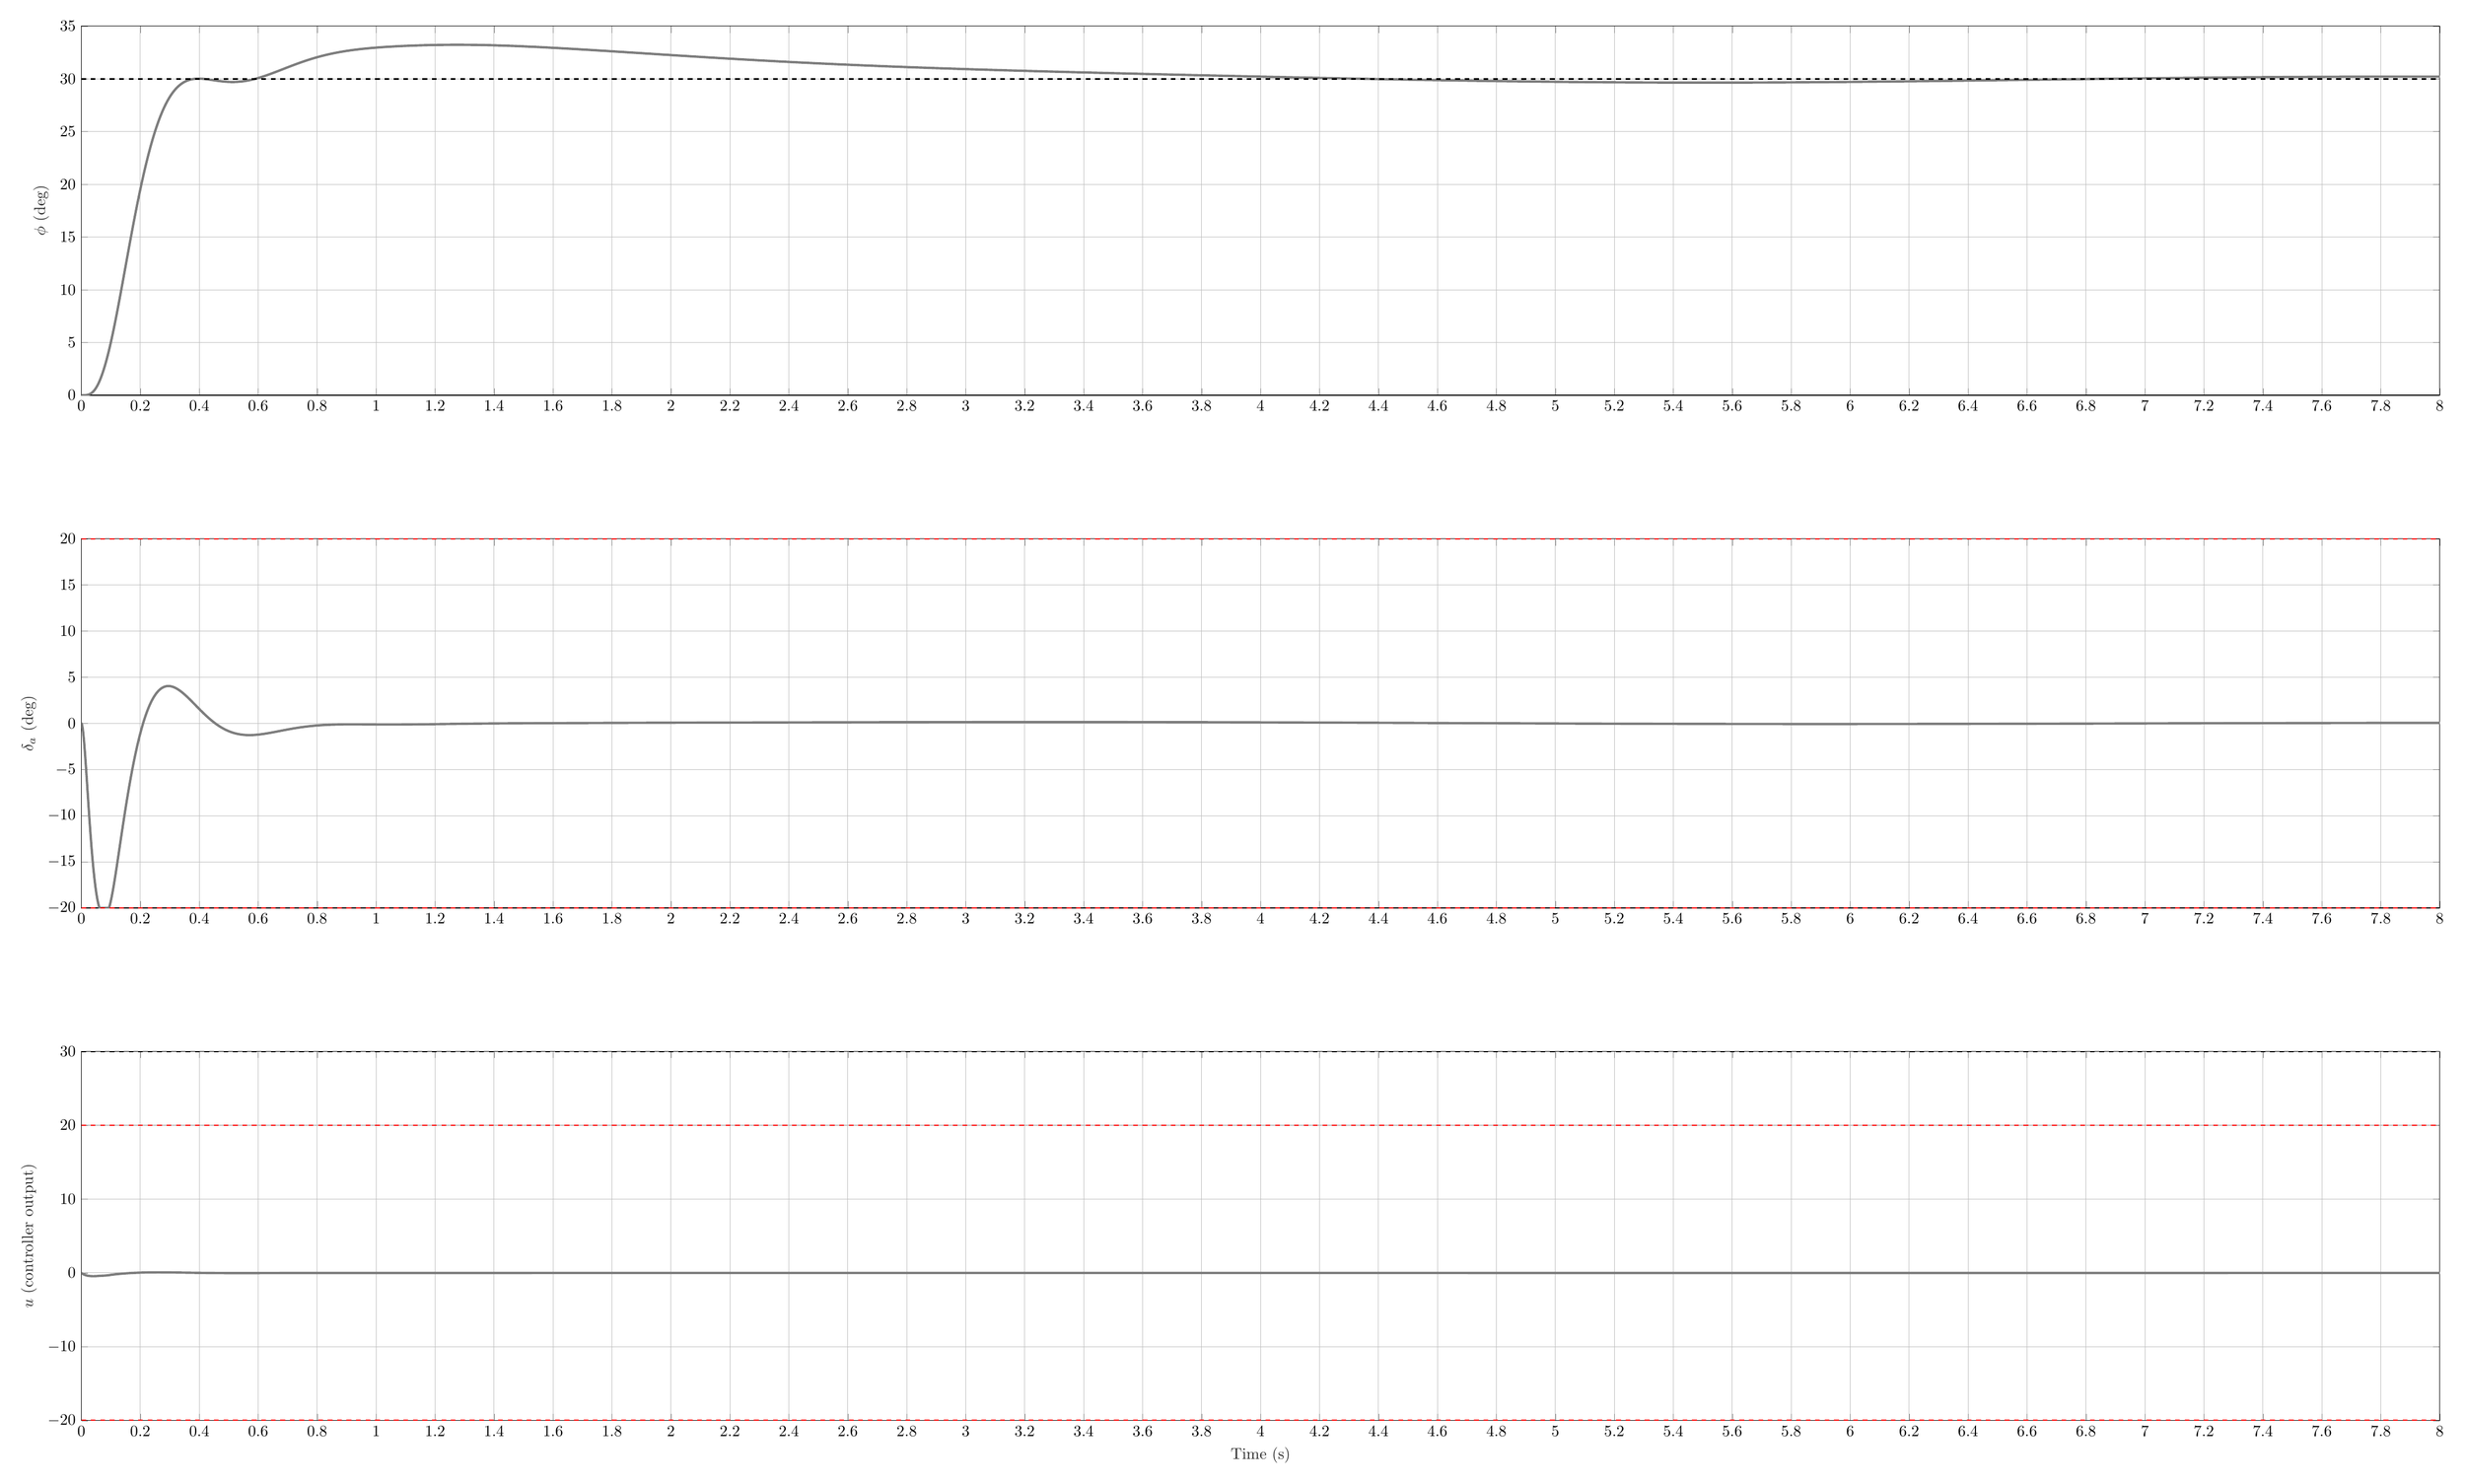
\begin{tikzpicture}

\begin{axis}[%
width=20.667in,
height=3.236in,
at={(3.467in,10.639in)},
scale only axis,
xmin=0,
xmax=8,
ymin=0,
ymax=35,
ylabel style={font=\color{white!15!black}},
ylabel={$\phi$ (deg)},
axis background/.style={fill=white},
xmajorgrids,
ymajorgrids
]
\addplot [color=mycolor1, line width=1.5pt, forget plot]
  table[row sep=crcr]{%
0	0\\
3.01259940762476e-05	2.21560527787266e-13\\
6.02519881524951e-05	3.62791889563652e-12\\
9.03779822287427e-05	1.839446841975e-11\\
0.00012050397630499	5.81137732689572e-11\\
0.000271133946686228	1.46667942888609e-09\\
0.000421763917067466	8.64497283226322e-09\\
0.000572393887448704	2.93225417383397e-08\\
0.000723023857829942	7.44681881032981e-08\\
0.00115007038637399	4.69470345646553e-07\\
0.00157711691491804	1.65405714943712e-06\\
0.00200416344346209	4.28991462324773e-06\\
0.00243120997200615	9.22046782714267e-06\\
0.0028588713994828	1.74857125907413e-05\\
0.00328653282695946	3.0296654908083e-05\\
0.00371419425443611	4.90319162433847e-05\\
0.00414185568191277	7.52230669943442e-05\\
0.00457612188145816	0.000111181333638605\\
0.00501038808100356	0.000158493795608568\\
0.00544465428054895	0.000219232555566133\\
0.00587892048009435	0.000295603597572817\\
0.00635993432740735	0.000401275236650951\\
0.00684094817472036	0.000532374975075744\\
0.00732196202203336	0.000692453657231686\\
0.00780297586934637	0.000885221840620794\\
0.00834383769594983	0.00114583636849004\\
0.00888469952255328	0.00145842896392501\\
0.00942556134915675	0.00182896496396478\\
0.00996642317576021	0.00226359943870751\\
0.0105310631377181	0.00279260041040144\\
0.0110957030996759	0.00340582905631485\\
0.0116603430616337	0.00411091629021293\\
0.0122249830235916	0.00491564758860078\\
0.0128027996084126	0.00585060370656253\\
0.0133806161932336	0.00690691625386764\\
0.0139584327780546	0.00809340009963664\\
0.0145362493628756	0.00941897196724188\\
0.0151284909382125	0.0109314150727919\\
0.0157207325135494	0.0126092902814476\\
0.0163129740888863	0.0144625036126118\\
0.0169052156642232	0.0165010093130792\\
0.0175128399618767	0.0187955240704106\\
0.0181204642595302	0.0213064822132363\\
0.0187280885571837	0.0240447667687686\\
0.0193357128548372	0.0270212537960052\\
0.019993664602274	0.0305254826523541\\
0.0206516163497107	0.0343355602896816\\
0.0213095680971475	0.0384652388496808\\
0.0219675198445842	0.0429281884007806\\
0.0226887585446486	0.0482194282969322\\
0.023409997244713	0.0539452747061062\\
0.0241312359447773	0.0601233631843951\\
0.0248524746448417	0.066771120743783\\
0.0256423799398331	0.0746110395853341\\
0.0264322852348246	0.0830573404031958\\
0.027222190529816	0.0921320281505784\\
0.0280120958248075	0.101856701539825\\
0.028877491412804	0.113281980644604\\
0.0297428870008006	0.125540220240675\\
0.0306082825887972	0.138658128262164\\
0.0314736781767937	0.152661710636846\\
0.032422875139768	0.169069849265944\\
0.0333720721027424	0.186606439838288\\
0.0343212690657167	0.205302898836346\\
0.035270466028691	0.225189512367428\\
0.0363138664234745	0.248457716890478\\
0.037357266818258	0.273236529650173\\
0.0384006672130415	0.29956151984431\\
0.039444067607825	0.327466519759978\\
0.0405866626757499	0.35987485017644\\
0.0417292577436747	0.394256295595661\\
0.0428718528115996	0.430648278994852\\
0.0440144478795245	0.46908571486366\\
0.0452294894743327	0.512240705789394\\
0.0464445310691409	0.557781466150541\\
0.0476595726639491	0.605740919316079\\
0.0488746142587574	0.656148900196797\\
0.0501701530850658	0.712623789027806\\
0.0514656919113743	0.771941558364148\\
0.0527612307376827	0.834127161969894\\
0.0540567695639912	0.899201850170775\\
0.0554404446987273	0.971914022931054\\
0.0568241198334634	1.04795867614641\\
0.0582077949681996	1.12734823336004\\
0.0595914701029357	1.21009080729805\\
0.0599404528345773	1.23148970395423\\
0.0602894355662189	1.25310217469078\\
0.0606384182978606	1.27492822235897\\
0.0609874010295022	1.29696783356188\\
0.0613363837611439	1.31922100252892\\
0.0616853664927855	1.3416876513729\\
0.0620343492244271	1.36436752783858\\
0.0623833319560687	1.38726022167433\\
0.0628466558260224	1.41798146757682\\
0.063309979695976	1.44907578818615\\
0.0637733035659296	1.48054203016148\\
0.0642366274358832	1.51237904370654\\
0.0648581083046427	1.55566393255539\\
0.0654795891734021	1.59961110565255\\
0.0661010700421616	1.64421781801498\\
0.066722550910921	1.68948133595919\\
0.0673698148309984	1.73731798734935\\
0.0680170787510759	1.7858610565592\\
0.0686643426711533	1.83510749430085\\
0.0693116065912307	1.8850542643558\\
0.070000870916635	1.93900861508291\\
0.0706901352420394	1.99375007243863\\
0.0713793995674437	2.0492750186516\\
0.072068663892848	2.10557985245551\\
0.0728038684798239	2.16649302018557\\
0.0735390730667997	2.22828509284553\\
0.0742742776537756	2.29095176184508\\
0.0750094822407515	2.35448873955098\\
0.0757959484886407	2.42341440572982\\
0.0765824147365299	2.49332589661376\\
0.077368880984419	2.56421804299967\\
0.0781553472323082	2.63608570256668\\
0.0789979797502578	2.71416255322368\\
0.0798406122682074	2.79334709778211\\
0.080683244786157	2.87363311385563\\
0.0815258773041066	2.95501441370844\\
0.0824279929827107	3.04334759723531\\
0.0833301086613147	3.13292160095411\\
0.0842322243399187	3.22372896339235\\
0.0851343400185227	3.31576226753428\\
0.0860950062679084	3.41510846146824\\
0.0870556725172941	3.51582768952172\\
0.0880163387666798	3.6179111600986\\
0.0889770050160655	3.7213501373505\\
0.0899867035628272	3.83152016357858\\
0.0909964021095889	3.9431679973984\\
0.0920061006563506	4.05628369386021\\
0.0930157992031123	4.17085737425912\\
0.093170341027759	4.18852175586566\\
0.0933248828524058	4.20622002798823\\
0.0934794246770526	4.22395215561616\\
0.0936339665016993	4.24171810377473\\
0.0937885083263461	4.25951783964144\\
0.0939430501509928	4.27735131843699\\
0.0940975919756396	4.29521847747463\\
0.0942521338002863	4.31311924099585\\
0.0944122421017475	4.33170013259017\\
0.0945723504032086	4.35031692501504\\
0.0947324587046697	4.3689695335081\\
0.0948925670061308	4.38765787278818\\
0.0956931085134365	4.4816325181403\\
0.0964936500207421	4.57648734545404\\
0.0972941915280477	4.6722111346449\\
0.0980947330353534	4.76879240066422\\
0.0996229689393587	4.95550464750897\\
0.101151204843364	5.14521433929577\\
0.102679440747369	5.33783412282831\\
0.104207676651375	5.53327456657945\\
0.105753895401694	5.73379178156241\\
0.107300114152013	5.93700509081332\\
0.108846332902332	6.14281557698451\\
0.110392551652651	6.35112333595837\\
0.111997694588381	6.56990304228339\\
0.11360283752411	6.79115062704145\\
0.115207980459839	7.01475109967581\\
0.116813123395568	7.2405893637466\\
0.118477402853009	7.47698766984123\\
0.12014168231045	7.71553871356453\\
0.12180596176789	7.95611391130756\\
0.123470241225331	8.19858543470754\\
0.125196641003569	8.45197514353052\\
0.126923040781806	8.70712710369258\\
0.128649440560044	8.96390120275411\\
0.130375840338281	9.22215891859215\\
0.132167620438292	9.49161932742996\\
0.133959400538304	9.76237856328572\\
0.135751180638315	10.0342871230378\\
0.137542960738326	10.3071979053346\\
0.139403675521435	10.591513922037\\
0.141264390304544	10.8765949378859\\
0.143125105087653	11.162284298494\\
0.144985819870762	11.4484285434079\\
0.146919109333348	11.7460540049947\\
0.148852398795933	12.043843005095\\
0.150785688258518	12.3416341770773\\
0.152718977721103	12.6392701247956\\
0.154728208221769	12.9482681863859\\
0.156737438722434	13.2567648335899\\
0.1587466692231	13.5645967646466\\
0.160755899723765	13.8716054086658\\
0.162843498857101	14.1895515232281\\
0.164931097990437	14.5062753512643\\
0.167018697123773	14.8216149556012\\
0.169106296257109	15.1354138635351\\
0.171272491697998	15.4592365670882\\
0.173438687138887	15.7810750376589\\
0.175604882579775	16.1007727548211\\
0.177771078020664	16.418179338723\\
0.180011431437259	16.7438884815277\\
0.182251784853853	17.066839789983\\
0.184492138270447	17.3868872214019\\
0.186732491687041	17.7038914240079\\
0.189032854403807	18.0260809093635\\
0.191333217120573	18.3447856586345\\
0.193633579837338	18.6598763883718\\
0.195933942554104	18.9712307948796\\
0.198259294444868	19.2820523976899\\
0.200584646335631	19.5888262127377\\
0.202909998226395	19.8914471932692\\
0.205235350117159	20.1898170489244\\
0.207500302349706	20.4762626812554\\
0.209765254582254	20.758509785786\\
0.212030206814801	21.0364856249532\\
0.214295159047349	21.3101230491776\\
0.21631136225085	21.5500082571351\\
0.218327565454352	21.786367072372\\
0.220343768657853	22.0191630785412\\
0.222359971861355	22.2483630792516\\
0.224902661844889	22.5322402461012\\
0.227445351828423	22.8102978383078\\
0.229988041811957	23.0824906283911\\
0.232530731795491	23.3487807026087\\
0.235481757276786	23.6503939377955\\
0.238432782758081	23.9439798093549\\
0.241383808239376	24.2295149200156\\
0.244334833720671	24.5069873673684\\
0.247635374321579	24.8077713720833\\
0.250935914922486	25.0984858422628\\
0.254236455523394	25.3791632308911\\
0.257536996124301	25.6498509249232\\
0.26110640813489	25.9314182751526\\
0.264675820145479	26.2014735921209\\
0.268245232156069	26.4601330227238\\
0.271814644166658	26.7075288016482\\
0.275567530825021	26.9556569493325\\
0.279320417483383	27.1916895414621\\
0.283073304141746	27.4158346036014\\
0.286826190800109	27.6283145976156\\
0.290701656493417	27.8357432772348\\
0.294577122186725	28.0312625548743\\
0.298452587880034	28.2151626348493\\
0.302328053573342	28.3877445581785\\
0.306299267738096	28.5531755070319\\
0.310270481902851	28.7073977033564\\
0.314241696067605	28.8507674516489\\
0.31821291023236	28.9836474474923\\
0.322071240220089	29.103053734198\\
0.325929570207819	29.2132517034445\\
0.329787900195549	29.314589262296\\
0.333646230183279	29.4074158635928\\
0.337049073784036	29.4825008389932\\
0.340451917384792	29.5514812231275\\
0.343854760985549	29.6145988963656\\
0.347257604586306	29.6720947961574\\
0.350011675469845	29.7146772145775\\
0.352765746353384	29.7538614569625\\
0.355519817236922	29.789773670789\\
0.358273888120461	29.8225390492852\\
0.361211795923381	29.8541626077585\\
0.364149703726302	29.8824963102722\\
0.367087611529222	29.9076882747731\\
0.370025519332142	29.9298847882598\\
0.373293435708585	29.9512315302119\\
0.376561352085028	29.9692471185252\\
0.379829268461471	29.9841245979306\\
0.383097184837913	29.9960534139962\\
0.386606266309874	30.0057914323078\\
0.390115347781835	30.0125696058975\\
0.393624429253795	30.0166084367733\\
0.397133510725756	30.0181228120034\\
0.400839654199142	30.0172126266677\\
0.404545797672527	30.0139601414423\\
0.408251941145913	30.0085981333139\\
0.411958084619299	30.0013517013852\\
0.415603737602884	29.992596134711\\
0.419249390586469	29.9824278331138\\
0.422895043570054	29.9710395709445\\
0.426540696553639	29.9586166428638\\
0.430293090955803	29.9449370044313\\
0.434045485357967	29.9305357120212\\
0.437797879760132	29.9155904208687\\
0.441550274162296	29.9002703801952\\
0.445386998961751	29.8843861982333\\
0.449223723761207	29.8684417398924\\
0.453060448560662	29.8525913042564\\
0.456897173360117	29.8369803064128\\
0.460399186135719	29.8230561953263\\
0.463901198911321	29.80954314992\\
0.467403211686923	29.7965328984432\\
0.470905224462525	29.7841113756731\\
0.474328032642741	29.7726166478707\\
0.477750840822957	29.7618305868103\\
0.481173649003173	29.7518178269222\\
0.484596457183389	29.7426381311792\\
0.488030045006324	29.7343217868334\\
0.491463632829259	29.7269496449082\\
0.494897220652194	29.7205677068709\\
0.498330808475128	29.7152175271198\\
0.501965801145464	29.710719050032\\
0.505600793815799	29.7074572132724\\
0.509235786486134	29.7054655972892\\
0.51287077915647	29.7047728892622\\
0.516663589495501	29.7054605722458\\
0.520456399834532	29.7076097646682\\
0.524249210173563	29.7112367141867\\
0.528042020512594	29.7163527684561\\
0.53196906203428	29.7232258673549\\
0.535896103555966	29.7317039563669\\
0.539823145077652	29.7417838094809\\
0.543750186599338	29.7534576459869\\
0.547800345171362	29.7671541608105\\
0.551850503743387	29.7825144799117\\
0.555900662315411	29.7995156706688\\
0.559950820887435	29.818130862122\\
0.56412160857819	29.8389548043893\\
0.568292396268946	29.8614196102208\\
0.572463183959701	29.8854836728699\\
0.576633971650457	29.9111022685222\\
0.580930374430174	29.939067386981\\
0.585226777209891	29.968575459375\\
0.589523179989608	29.9995680204823\\
0.593819582769325	30.0319844627604\\
0.598277548256071	30.0670579290134\\
0.602735513742817	30.1035240828813\\
0.607193479229564	30.141308650767\\
0.61165144471631	30.1803362948751\\
0.616298917859053	30.2222639457574\\
0.620946391001795	30.2653714593423\\
0.625593864144537	30.3095704361331\\
0.63024133728728	30.3547726591585\\
0.635126612062361	30.4032727833622\\
0.640011886837442	30.4526816849248\\
0.644897161612523	30.5028980645663\\
0.649782436387604	30.5538222772562\\
0.654794576314306	30.6067017710594\\
0.659806716241009	30.6601185627496\\
0.664818856167712	30.713970697025\\
0.669830996094415	30.7681592099248\\
0.674903184975336	30.8232411704961\\
0.679975373856258	30.8784723036058\\
0.685047562737179	30.9337593322122\\
0.6901197516181	30.9890128781135\\
0.695305729310734	31.0453821967452\\
0.700491707003367	31.1015393194699\\
0.705677684696001	31.1574010337504\\
0.710863662388635	31.2128887826904\\
0.716218865161277	31.2697161758602\\
0.72157406793392	31.3259891328743\\
0.726929270706563	31.3816361926665\\
0.732284473479205	31.4365912067913\\
0.737743625929434	31.4918374534406\\
0.743202778379663	31.5462418519662\\
0.748661930829891	31.599750559897\\
0.75412108328012	31.6523151028162\\
0.759214740193208	31.7004707232892\\
0.764308397106296	31.7477355253256\\
0.769402054019384	31.79408210284\\
0.774495710932471	31.8394866445505\\
0.779456426834987	31.8827813224013\\
0.784417142737503	31.9251476607074\\
0.789377858640018	31.9665729738077\\
0.794338574542534	32.0070473145513\\
0.799276567701765	32.0463846097698\\
0.804214560860997	32.0847679162469\\
0.809152554020228	32.1221950492058\\
0.814090547179459	32.158665992031\\
0.819069611455796	32.1944742757294\\
0.824048675732133	32.2293169423127\\
0.829027740008469	32.2632002521221\\
0.834006804284806	32.2961321633983\\
0.839078436902364	32.3287082036197\\
0.844150069519923	32.3603191511229\\
0.849221702137481	32.3909784640658\\
0.85429333475504	32.420700864944\\
0.859508832583604	32.4503060597353\\
0.864724330412168	32.4789561507394\\
0.869939828240732	32.506670981179\\
0.875155326069296	32.5334712269497\\
0.880574378983997	32.5603717156672\\
0.885993431898699	32.5863332204489\\
0.8914124848134	32.6113814795563\\
0.896831537728101	32.6355426041263\\
0.902533602193041	32.6600368148094\\
0.908235666657981	32.6836095862596\\
0.91393773112292	32.706292420203\\
0.91963979558786	32.7281166630593\\
0.925746754748153	32.750573838653\\
0.931853713908446	32.7721203110425\\
0.937960673068739	32.7927938310053\\
0.944067632229032	32.8126313192897\\
0.950806501603583	32.8335945619266\\
0.957545370978134	32.8536314949202\\
0.964284240352685	32.8727882158225\\
0.971023109727236	32.8911089544067\\
0.97901042188167	32.9117994133488\\
0.986997734036105	32.9314429497648\\
0.99498504619054	32.9501035439042\\
1.00297235834497	32.9678408393194\\
1.01135983109742	32.9855337631172\\
1.01974730384986	33.0023300468056\\
1.02813477660231	33.0182848214761\\
1.03652224935475	33.0334481555094\\
1.04439928228509	33.0470085641547\\
1.05227631521543	33.0599450719368\\
1.06015334814577	33.0722882931771\\
1.06803038107612	33.0840655767833\\
1.0753144779759	33.0944737785036\\
1.08259857487569	33.1044356964349\\
1.08988267177547	33.1139662445153\\
1.09716676867525	33.1230785302104\\
1.10437223838645	33.1316920847595\\
1.11157770809764	33.1399167973671\\
1.11878317780883	33.1477606296073\\
1.12598864752002	33.1552303570949\\
1.13332815742251	33.162460240643\\
1.14066766732501	33.1693124557762\\
1.1480071772275	33.1757907452901\\
1.15534668713	33.1818981131235\\
1.16297547430514	33.1878554900519\\
1.17060426148028	33.1934162093211\\
1.17823304865542	33.1985813863447\\
1.18586183583056	33.2033518065135\\
1.19396238949679	33.207985589869\\
1.20206294316303	33.2121747506736\\
1.21016349682926	33.2159191707291\\
1.2182640504955	33.2192188311812\\
1.22712548175832	33.2223190895204\\
1.23598691302114	33.2248870966689\\
1.24484834428396	33.2269232129772\\
1.25370977554678	33.2284284265993\\
1.26398693377755	33.2295112603107\\
1.27426409200831	33.2298850438113\\
1.28454125023907	33.2295540268144\\
1.29481840846984	33.2285239838197\\
1.30729397615686	33.2263445714555\\
1.31976954384389	33.2231602151034\\
1.33224511153092	33.2189883957817\\
1.34472067921795	33.2138495831473\\
1.35624324173877	33.2082640833974\\
1.36776580425959	33.2018926330662\\
1.37928836678041	33.1947562220837\\
1.39081092930122	33.1868770513532\\
1.40131675044724	33.1790654437279\\
1.41182257159325	33.1706740127224\\
1.42232839273927	33.1617215153064\\
1.43283421388528	33.1522269560716\\
1.44355466690838	33.1419995932383\\
1.45427511993147	33.1312485421689\\
1.46499557295456	33.1199944874124\\
1.47571602597766	33.1082579052237\\
1.48715746781825	33.0952225742532\\
1.49859890965885	33.0816852827629\\
1.51004035149944	33.0676700670355\\
1.52148179334004	33.0532002889504\\
1.53431438775102	33.0364584590874\\
1.547146982162	33.0192048110224\\
1.55997957657298	33.0014695592306\\
1.57281217098397	32.983281576322\\
1.58900854664744	32.9597225465357\\
1.60520492231092	32.9355396848586\\
1.6214012979744	32.9107832987625\\
1.63759767363788	32.8855004758367\\
1.65587342003588	32.8563950325873\\
1.67414916643388	32.8267358028755\\
1.69242491283187	32.7965788913121\\
1.71070065922987	32.7659768713545\\
1.72598910726814	32.7400709992978\\
1.74127755530641	32.7139155836201\\
1.75656600334469	32.6875366791083\\
1.77185445138296	32.6609593223998\\
1.78801406233123	32.6326783810288\\
1.8041736732795	32.6042294867802\\
1.82033328422778	32.5756385723751\\
1.83649289517605	32.5469307269858\\
1.85529182332338	32.5134189687463\\
1.87409075147071	32.4798178283701\\
1.89288967961804	32.4461620486632\\
1.91168860776537	32.4124851143833\\
1.93605030322665	32.3688635962242\\
1.96041199868792	32.3253257543844\\
1.9847736941492	32.2819332446889\\
2.00913538961047	32.2387440420909\\
2.03201000043149	32.1984243349003\\
2.05488461125251	32.1583724116062\\
2.07775922207353	32.1186263675141\\
2.10063383289455	32.0792211793858\\
2.12444214793938	32.0386038847902\\
2.14825046298421	31.9984230194016\\
2.17205877802904	31.9587078786905\\
2.19586709307387	31.9194845242176\\
2.22287535705472	31.8756137299727\\
2.24988362103557	31.8324342283805\\
2.27689188501642	31.78997043901\\
2.30390014899727	31.7482426861005\\
2.33028504812221	31.7082044889989\\
2.35666994724715	31.6688959541853\\
2.38305484637209	31.6303256214129\\
2.40943974549703	31.5924993525684\\
2.43539773858392	31.5560142852255\\
2.46135573167082	31.5202527677255\\
2.48731372475771	31.485213048635\\
2.51327171784461	31.4508915359329\\
2.53839484463513	31.4183526597977\\
2.56351797142566	31.3864746655591\\
2.58864109821618	31.3552495044773\\
2.6137642250067	31.324667958657\\
2.64006175836685	31.2933349612975\\
2.666359291727	31.262682376095\\
2.69265682508714	31.2326957513973\\
2.71895435844729	31.203359685706\\
2.7366592922277	31.1839673239261\\
2.75436422600811	31.1648572345848\\
2.77206915978852	31.1460240572566\\
2.78977409356893	31.1274623315606\\
2.80747902734934	31.1091664736299\\
2.82518396112975	31.0911307560989\\
2.84288889491015	31.0733493835114\\
2.86059382869056	31.0558165005963\\
2.88883395014664	31.0283503856991\\
2.91707407160271	31.0014770596555\\
2.94531419305879	30.9751720131432\\
2.97355431451486	30.9494106372999\\
2.98780028373157	30.9366136093666\\
3.00204625294828	30.9239455466118\\
3.016292222165	30.9114033078383\\
3.03053819138171	30.8989837850573\\
3.04478416059842	30.8866838834922\\
3.05903012981513	30.8745005105576\\
3.07327609903184	30.8624306083099\\
3.08752206824856	30.8504711479417\\
3.1224828009256	30.8215710496835\\
3.15744353360264	30.7932744747203\\
3.19240426627968	30.7655390900238\\
3.22736499895673	30.7383242898965\\
3.24895007301778	30.7217645021721\\
3.27053514707883	30.7053793599531\\
3.29212022113988	30.689160271095\\
3.31370529520094	30.6730989383517\\
3.33529036926199	30.6571873820523\\
3.35687544332304	30.6414178374527\\
3.37846051738409	30.6257828706906\\
3.40004559144514	30.6102754743307\\
3.41561288897728	30.5991668229612\\
3.43118018650941	30.5881185647703\\
3.44674748404154	30.5771283691817\\
3.46231478157368	30.5661939734212\\
3.47788207910581	30.555313212942\\
3.49344937663794	30.5444840346122\\
3.50901667417008	30.5337044629698\\
3.52458397170221	30.5229726150041\\
3.55163340276777	30.504433429597\\
3.57868283383334	30.486024240893\\
3.6057322648989	30.4677371541705\\
3.63278169596446	30.4495651625011\\
3.65179320185695	30.436858609014\\
3.67080470774944	30.4242039250997\\
3.68981621364193	30.4115994144627\\
3.70882771953442	30.3990435564313\\
3.72783922542691	30.3865350351954\\
3.7468507313194	30.3740727578049\\
3.76586223721189	30.3616558067977\\
3.78487374310438	30.3492834476474\\
3.81119132703964	30.3322290780961\\
3.83750891097489	30.3152582554403\\
3.86382649491014	30.298370722336\\
3.8901440788454	30.2815670654113\\
3.90371577019078	30.2729347446173\\
3.91728746153616	30.2643251970912\\
3.93085915288154	30.2557386843132\\
3.94443084422693	30.2471754913475\\
3.95800253557231	30.2386359479301\\
3.97157422691769	30.2301204387141\\
3.98514591826308	30.2216293762902\\
3.99871760960846	30.2131632098653\\
4.02809086517373	30.1949274594434\\
4.05746412073901	30.1768161831317\\
4.08683737630428	30.158835654236\\
4.11621063186956	30.1409928257669\\
4.14373369811461	30.1244056332701\\
4.17125676435966	30.1079528304434\\
4.19877983060472	30.0916416441064\\
4.22630289684977	30.0754797229192\\
4.24694074777543	30.0634636308818\\
4.26757859870109	30.0515394748054\\
4.28821644962676	30.0397108713108\\
4.30885430055242	30.027981520388\\
4.32949215147808	30.0163551931045\\
4.35013000240374	30.0048358031424\\
4.37076785332941	29.9934273149388\\
4.39140570425507	29.9821336769274\\
4.40767819869046	29.9733125093028\\
4.42395069312586	29.9645672782284\\
4.44022318756125	29.9558999981179\\
4.45649568199665	29.9473127205946\\
4.47276817643204	29.9388074995695\\
4.48904067086743	29.930386377277\\
4.50531316530283	29.922051416907\\
4.52158565973822	29.9138046832141\\
4.54710398716749	29.9010548518026\\
4.57262231459675	29.8885350510163\\
4.59814064202602	29.8762532377544\\
4.62365896945528	29.8642172685687\\
4.64107841586567	29.8561464197162\\
4.65849786227607	29.8481962484656\\
4.67591730868646	29.8403691947998\\
4.69333675509686	29.8326676909076\\
4.71075620150725	29.825094135584\\
4.72817564791765	29.8176508845173\\
4.74559509432804	29.8103402715022\\
4.76301454073844	29.8031645931489\\
4.78955621462285	29.7924956481092\\
4.81609788850726	29.7821530372988\\
4.84263956239167	29.7721443658531\\
4.86918123627608	29.7624768964987\\
4.88517871422827	29.7568177732884\\
4.90117619218047	29.7512866690205\\
4.91717367013267	29.7458850297377\\
4.93317114808487	29.7406142795698\\
4.94916862603706	29.7354757941598\\
4.96516610398926	29.7304708893748\\
4.98116358194146	29.7256008484692\\
4.99716105989366	29.72086690833\\
5.02541962351935	29.7128408406246\\
5.05367818714505	29.7052493429167\\
5.08193675077075	29.6980981461143\\
5.11019531439644	29.6913924125669\\
5.12665189748672	29.6876944002768\\
5.143108480577	29.6841499153689\\
5.15956506366727	29.680759736306\\
5.17602164675755	29.6775245943005\\
5.19247822984783	29.6744451528466\\
5.2089348129381	29.6715219985715\\
5.22539139602838	29.6687556636711\\
5.24184797911866	29.6661466159701\\
5.27199678378995	29.6617760737851\\
5.30214558846124	29.6579366606171\\
5.33229439313253	29.65462956043\\
5.36244319780382	29.6518550973156\\
5.37742141120313	29.6506746623857\\
5.39239962460245	29.649625509135\\
5.40737783800177	29.6487074707556\\
5.42235605140108	29.6479203479496\\
5.4373342648004	29.6472638910504\\
5.45231247819972	29.6467377916792\\
5.46729069159903	29.6463417040163\\
5.48226890499835	29.6460752367924\\
5.51702285317393	29.645953726636\\
5.55177680134952	29.6465212073896\\
5.5865307495251	29.6477699623842\\
5.62128469770068	29.6496908985225\\
5.63729885829491	29.650799453313\\
5.65331301888913	29.6520474604583\\
5.66932717948336	29.6534337585917\\
5.68534134007759	29.6549571407192\\
5.70135550067181	29.6566163423453\\
5.71736966126604	29.6584100343214\\
5.73338382186026	29.6603368409399\\
5.74939798245449	29.6623953364752\\
5.77983276161503	29.6666650916849\\
5.81026754077558	29.6713944429924\\
5.84070231993612	29.6765720874309\\
5.87113709909667	29.6821860258527\\
5.88761126838737	29.6854023918591\\
5.90408543767808	29.6887408657757\\
5.92055960696879	29.6921993283482\\
5.9370337762595	29.6957756238666\\
5.9535079455502	29.6994675473618\\
5.96998211484091	29.7032728346498\\
5.98645628413162	29.7071891859697\\
6.00293045342232	29.7112142643795\\
6.0304711718378	29.718179469343\\
6.05801189025328	29.7254304858243\\
6.08555260866876	29.7329556463227\\
6.11309332708423	29.7407429406843\\
6.13015189095704	29.7456924565261\\
6.14721045482985	29.7507349072502\\
6.16426901870267	29.7558672976238\\
6.18132758257548	29.7610866120548\\
6.19838614644829	29.7663898017992\\
6.2154447103211	29.7717737712179\\
6.23250327419391	29.7772354072765\\
6.24956183806672	29.782771581168\\
6.27740623599313	29.7919600634253\\
6.30525063391953	29.8013248613702\\
6.33309503184594	29.8108520010105\\
6.36093942977234	29.8205272731331\\
6.37651431324539	29.8259984728649\\
6.39208919671843	29.8315090891014\\
6.40766408019148	29.8370566081176\\
6.42323896366452	29.8426385223458\\
6.43881384713757	29.8482523180354\\
6.45438873061062	29.853895466444\\
6.46996361408366	29.8595654457193\\
6.48553849755671	29.8652597387883\\
6.5126803911338	29.8752336072523\\
6.53982228471088	29.885260336453\\
6.56696417828797	29.8953266395966\\
6.59410607186506	29.9054192534435\\
6.6134220296676	29.912610585425\\
6.63273798747014	29.9198038507729\\
6.65205394527268	29.9269943465301\\
6.67136990307522	29.9341774070102\\
6.69068586087776	29.9413484024528\\
6.7100018186803	29.9485027026467\\
6.72931777648283	29.955635726902\\
6.74863373428537	29.9627429714873\\
6.77149672864303	29.9711158580451\\
6.79435972300068	29.9794390020314\\
6.81722271735834	29.9877051804546\\
6.84008571171599	29.9959071538062\\
6.85847006625643	30.0024510602057\\
6.87685442079687	30.0089453085946\\
6.89523877533731	30.0153863289648\\
6.91362312987775	30.0217706199459\\
6.93054876563024	30.0275952219363\\
6.94747440138273	30.0333661364045\\
6.96440003713522	30.0390807402864\\
6.98132567288771	30.0447364865609\\
7.0010118012876	30.0512372756155\\
7.02069792968748	30.0576511256367\\
7.04038405808737	30.0639742328694\\
7.06007018648726	30.0702028426642\\
7.07956767778404	30.0762750379826\\
7.09906516908083	30.0822475267804\\
7.11856266037761	30.0881169447675\\
7.1380601516744	30.0938800265493\\
7.15923942510662	30.1000160376121\\
7.18041869853883	30.1060188632412\\
7.20159797197105	30.1118846691495\\
7.22277724540327	30.1176098261483\\
7.23895673655392	30.1218864965502\\
7.25513622770458	30.1260774923855\\
7.27131571885523	30.1301813493311\\
7.28749521000589	30.1341966269918\\
7.30367470115654	30.1381219424974\\
7.3198541923072	30.1419559842809\\
7.33603368345785	30.1456974755122\\
7.35221317460851	30.1493451909139\\
7.37753160786677	30.1548623440235\\
7.40285004112502	30.1601427443921\\
7.42816847438328	30.1651824406917\\
7.45348690764154	30.1699778260251\\
7.4713688848096	30.1732157012738\\
7.48925086197767	30.1763289700708\\
7.50713283914573	30.1793166439015\\
7.52501481631379	30.1821777936745\\
7.54289679348186	30.1849115759084\\
7.56077877064992	30.1875172429072\\
7.57866074781798	30.1899941134639\\
7.59654272498605	30.1923415858892\\
7.62211964712593	30.1954733100941\\
7.64769656926582	30.1983379882905\\
7.6732734914057	30.2009346758317\\
7.69885041354559	30.2032628195639\\
7.71466601023124	30.2045679461278\\
7.7304816069169	30.205770273733\\
7.74629720360255	30.2068698536898\\
7.7621128002882	30.2078667646235\\
7.77792839697386	30.2087611374536\\
7.79374399365951	30.209553166447\\
7.80955959034517	30.2102430795291\\
7.82537518703082	30.2108311496814\\
7.85355084323973	30.2116275014581\\
7.88172649944864	30.2121038061639\\
7.90990215565755	30.2122626453104\\
7.93807781186646	30.2121070702403\\
7.95355835889985	30.2118889990234\\
7.96903890593323	30.2115776734108\\
7.98451945296662	30.2111737610787\\
8	30.2106779578723\\
};
\addplot [color=black, dashed, line width=1.0pt, forget plot]
  table[row sep=crcr]{%
0	30\\
8	30\\
};
\end{axis}

\begin{axis}[%
width=20.667in,
height=3.236in,
at={(3.467in,6.144in)},
scale only axis,
xmin=0,
xmax=8,
ymin=-20,
ymax=20,
ylabel style={font=\color{white!15!black}},
ylabel={$\delta_a$ (deg)},
axis background/.style={fill=white},
xmajorgrids,
ymajorgrids
]
\addplot [color=mycolor1, line width=1.5pt, forget plot]
  table[row sep=crcr]{%
0	0\\
3.01259940762476e-05	-2.75298387417236e-05\\
6.02519881524951e-05	-0.000110022826593854\\
9.03779822287427e-05	-0.000247334365468926\\
0.00012050397630499	-0.000439320116575602\\
0.000271133946686228	-0.00221432786020752\\
0.000421763917067466	-0.00533468898385212\\
0.000572393887448704	-0.00978265120627718\\
0.000723023857829942	-0.0155406205701218\\
0.00115007038637399	-0.0388343014878632\\
0.00157711691491804	-0.0721274888109862\\
0.00200416344346209	-0.115039679590709\\
0.00243120997200615	-0.167199890571575\\
0.0028588713994828	-0.228340784735897\\
0.00328653282695946	-0.298040448872625\\
0.00371419425443611	-0.375954520500133\\
0.00414185568191277	-0.461747411173345\\
0.00457612188145816	-0.556591435016281\\
0.00501038808100356	-0.658889676112544\\
0.00544465428054895	-0.768318056764668\\
0.00587892048009435	-0.8845610313375\\
0.00635993432740735	-1.02090070942039\\
0.00684094817472036	-1.16481967051184\\
0.00732196202203336	-1.31592506559974\\
0.00780297586934637	-1.47383568928145\\
0.00834383769594983	-1.65906227101109\\
0.00888469952255328	-1.85191822076105\\
0.00942556134915675	-2.05191324870614\\
0.00996642317576021	-2.2585737160548\\
0.0105310631377181	-2.48093657064833\\
0.0110957030996759	-2.70956553313132\\
0.0116603430616337	-2.94397855263367\\
0.0122249830235916	-3.18371112294523\\
0.0128027996084126	-3.43407913995484\\
0.0133806161932336	-3.68909018921937\\
0.0139584327780546	-3.94830230013098\\
0.0145362493628756	-4.21129048099205\\
0.0151284909382125	-4.48433587353174\\
0.0157207325135494	-4.76049911826546\\
0.0163129740888863	-5.03937688008082\\
0.0169052156642232	-5.32058227409233\\
0.0175128399618767	-5.61112249934433\\
0.0181204642595302	-5.9033412356966\\
0.0187280885571837	-6.1968734046451\\
0.0193357128548372	-6.49136983656198\\
0.019993664602274	-6.81095991247682\\
0.0206516163497107	-7.13088836394045\\
0.0213095680971475	-7.45077339054841\\
0.0219675198445842	-7.77025204084124\\
0.0226887585446486	-8.11958619974289\\
0.023409997244713	-8.46759222325446\\
0.0241312359447773	-8.81386797502129\\
0.0248524746448417	-9.1580343577209\\
0.0256423799398331	-9.53212652678009\\
0.0264322852348246	-9.90282673861993\\
0.027222190529816	-10.2697293494616\\
0.0280120958248075	-10.6324561866146\\
0.028877491412804	-11.0246402517023\\
0.0297428870008006	-11.4109699118996\\
0.0306082825887972	-11.79105794497\\
0.0314736781767937	-12.1645491117511\\
0.032422875139768	-12.5662388087379\\
0.0333720721027424	-12.9592237444594\\
0.0343212690657167	-13.3431636216859\\
0.035270466028691	-13.7177544173506\\
0.0363138664234745	-14.1184167467777\\
0.037357266818258	-14.5071576954962\\
0.0384006672130415	-14.8837200722667\\
0.039444067607825	-15.2478865981791\\
0.0405866626757499	-15.6322459421113\\
0.0417292577436747	-16.001355666018\\
0.0428718528115996	-16.3550895940152\\
0.0440144478795245	-16.6933626950403\\
0.0452294894743327	-17.036074143827\\
0.0464445310691409	-17.3612581807846\\
0.0476595726639491	-17.6689609369387\\
0.0488746142587574	-17.9592641616252\\
0.0501701530850658	-18.2497672515913\\
0.0514656919113743	-18.5208181002821\\
0.0527612307376827	-18.7726457327919\\
0.0540567695639912	-19.0055077596747\\
0.0554404446987273	-19.2335918911583\\
0.0568241198334634	-19.4407635379476\\
0.0582077949681996	-19.6274419857939\\
0.0595914701029357	-19.7940662814366\\
0.0599404528345773	-19.832978652524\\
0.0602894355662189	-19.8706524253349\\
0.0606384182978606	-19.9070953081307\\
0.0609874010295022	-19.9423150716782\\
0.0613363837611439	-19.9763173856107\\
0.0616853664927855	-20\\
0.0620343492244271	-20\\
0.0623833319560687	-20\\
0.0628466558260224	-20\\
0.063309979695976	-20\\
0.0637733035659296	-20\\
0.0642366274358832	-20\\
0.0648581083046427	-20\\
0.0654795891734021	-20\\
0.0661010700421616	-20\\
0.066722550910921	-20\\
0.0673698148309984	-20\\
0.0680170787510759	-20\\
0.0686643426711533	-20\\
0.0693116065912307	-20\\
0.070000870916635	-20\\
0.0706901352420394	-20\\
0.0713793995674437	-20\\
0.072068663892848	-20\\
0.0728038684798239	-20\\
0.0735390730667997	-20\\
0.0742742776537756	-20\\
0.0750094822407515	-20\\
0.0757959484886407	-20\\
0.0765824147365299	-20\\
0.077368880984419	-20\\
0.0781553472323082	-20\\
0.0789979797502578	-20\\
0.0798406122682074	-20\\
0.080683244786157	-20\\
0.0815258773041066	-20\\
0.0824279929827107	-20\\
0.0833301086613147	-20\\
0.0842322243399187	-20\\
0.0851343400185227	-20\\
0.0860950062679084	-20\\
0.0870556725172941	-20\\
0.0880163387666798	-20\\
0.0889770050160655	-20\\
0.0899867035628272	-20\\
0.0909964021095889	-20\\
0.0920061006563506	-20\\
0.0930157992031123	-20\\
0.093170341027759	-20\\
0.0933248828524058	-20\\
0.0934794246770526	-20\\
0.0936339665016993	-20\\
0.0937885083263461	-20\\
0.0939430501509928	-19.9849134197161\\
0.0940975919756396	-19.9695608374675\\
0.0942521338002863	-19.9539976893204\\
0.0944122421017475	-19.9376543326418\\
0.0945723504032086	-19.9210892739035\\
0.0947324587046697	-19.9043045395286\\
0.0948925670061308	-19.887302141614\\
0.0956931085134365	-19.7990947453962\\
0.0964936500207421	-19.7057393820849\\
0.0972941915280477	-19.6074718209098\\
0.0980947330353534	-19.5045197907324\\
0.0996229689393587	-19.2957678172406\\
0.101151204843364	-19.0721860200856\\
0.102679440747369	-18.8351248030776\\
0.104207676651375	-18.5858507091447\\
0.105753895401694	-18.3224208557736\\
0.107300114152013	-18.0488283045215\\
0.108846332902332	-17.7661291415177\\
0.110392551652651	-17.475312246065\\
0.111997694588381	-17.165810686085\\
0.11360283752411	-16.8495000676896\\
0.115207980459839	-16.5272624685562\\
0.116813123395568	-16.199921183794\\
0.118477402853009	-15.8559462306926\\
0.12014168231045	-15.5080832980246\\
0.12180596176789	-15.1570543779081\\
0.123470241225331	-14.8035311182795\\
0.125196641003569	-14.4348395603837\\
0.126923040781806	-14.0647602817404\\
0.128649440560044	-13.693874656023\\
0.130375840338281	-13.3227215702765\\
0.132167620438292	-12.9377595913437\\
0.133959400538304	-12.5535425031946\\
0.135751180638315	-12.1705299507107\\
0.137542960738326	-11.7891462438053\\
0.139403675521435	-11.3952290409159\\
0.141264390304544	-11.0038752599492\\
0.143125105087653	-10.6154405422052\\
0.144985819870762	-10.2302515471581\\
0.146919109333348	-9.83379470137709\\
0.148852398795933	-9.44145632783449\\
0.150785688258518	-9.05350403578957\\
0.152718977721103	-8.67018195867476\\
0.154728208221769	-8.27694473559853\\
0.156737438722434	-7.88916087932397\\
0.1587466692231	-7.50702379834456\\
0.160755899723765	-7.13070807301295\\
0.162843498857101	-6.7460465778754\\
0.164931097990437	-6.36798448179815\\
0.167018697123773	-5.99665247388732\\
0.169106296257109	-5.63216622883193\\
0.171272491697998	-5.261301180213\\
0.173438687138887	-4.89800536889442\\
0.175604882579775	-4.54235589850133\\
0.177771078020664	-4.1944179003722\\
0.180011431437259	-3.84273606159784\\
0.182251784853853	-3.49940034360082\\
0.184492138270447	-3.16444139093666\\
0.186732491687041	-2.83788025512336\\
0.189032854403807	-2.51132144251183\\
0.191333217120573	-2.19362671003344\\
0.193633579837338	-1.88478634610762\\
0.195933942554104	-1.58478293301999\\
0.198259294444868	-1.29047581555523\\
0.200584646335631	-1.00513650320141\\
0.202909998226395	-0.728722304412775\\
0.205235350117159	-0.461184470204177\\
0.207500302349706	-0.209076756675433\\
0.209765254582254	0.0347193687381411\\
0.212030206814801	0.270265882914817\\
0.214295159047349	0.49762905041801\\
0.21631136225085	0.693194646380356\\
0.218327565454352	0.882384748780443\\
0.220343768657853	1.06525475281939\\
0.222359971861355	1.24186226582943\\
0.224902661844889	1.45575087231912\\
0.227445351828423	1.65990002056048\\
0.229988041811957	1.85443998153334\\
0.232530731795491	2.03950540709456\\
0.235481757276786	2.24259577174369\\
0.238432782758081	2.433337143536\\
0.241383808239376	2.61196166784088\\
0.244334833720671	2.77870738856258\\
0.247635374321579	2.95143041044821\\
0.250935914922486	3.10995038491635\\
0.254236455523394	3.25462539775893\\
0.257536996124301	3.38581965266868\\
0.26110640813489	3.51295685568301\\
0.264675820145479	3.62523785947252\\
0.268245232156069	3.72314543261145\\
0.271814644166658	3.80716649732601\\
0.275567530825021	3.88106952440697\\
0.279320417483383	3.94074096218734\\
0.283073304141746	3.98675893025022\\
0.286826190800109	4.0197016594806\\
0.290701656493417	4.04061112719912\\
0.294577122186725	4.04883172047035\\
0.298452587880034	4.04499787955456\\
0.302328053573342	4.02973903595239\\
0.306299267738096	4.00290442288315\\
0.310270481902851	3.96539637702824\\
0.314241696067605	3.91787356563873\\
0.31821291023236	3.8609843264874\\
0.322071240220089	3.79734692317735\\
0.325929570207819	3.72604743442113\\
0.329787900195549	3.6476513446966\\
0.333646230183279	3.56271170793917\\
0.337049073784036	3.4828005462459\\
0.340451917384792	3.3985841297969\\
0.343854760985549	3.31041759901299\\
0.347257604586306	3.21864733816892\\
0.350011675469845	3.14196690490254\\
0.352765746353384	3.06332238467755\\
0.355519817236922	2.98288484124298\\
0.358273888120461	2.90082129504029\\
0.361211795923381	2.81167110567813\\
0.364149703726302	2.72104896018423\\
0.367087611529222	2.62914240454092\\
0.370025519332142	2.53613350719335\\
0.373293435708585	2.4315971894095\\
0.376561352085028	2.3261507059587\\
0.379829268461471	2.22002091682642\\
0.383097184837913	2.11342612925692\\
0.386606266309874	1.99868635836138\\
0.390115347781835	1.88390137233217\\
0.393624429253795	1.769309021507\\
0.397133510725756	1.65513589298482\\
0.400839654199142	1.53524442472161\\
0.404545797672527	1.41630133628809\\
0.408251941145913	1.29853354905825\\
0.411958084619299	1.18215451994371\\
0.415603737602884	1.06922421997325\\
0.419249390586469	0.958009533641658\\
0.422895043570054	0.848676552079165\\
0.426540696553639	0.741379603503737\\
0.430293090955803	0.63321783569777\\
0.434045485357967	0.527507023179487\\
0.437797879760132	0.424377625648705\\
0.441550274162296	0.323948110800047\\
0.445386998961751	0.224164157464813\\
0.449223723761207	0.127415409695323\\
0.453060448560662	0.033791017504677\\
0.456897173360117	-0.0566314174003921\\
0.460399186135719	-0.136314072169269\\
0.463901198911321	-0.213231828736446\\
0.467403211686923	-0.287349918074247\\
0.470905224462525	-0.358640483532722\\
0.474328032642741	-0.425566175891517\\
0.477750840822957	-0.489757467420288\\
0.481173649003173	-0.551206743676545\\
0.484596457183389	-0.609911721301559\\
0.488030045006324	-0.666047327323856\\
0.491463632829259	-0.719432786977673\\
0.494897220652194	-0.770081272012472\\
0.498330808475128	-0.818010380261741\\
0.501965801145464	-0.865812037190878\\
0.505600793815799	-0.91062215816437\\
0.509235786486134	-0.952477026528493\\
0.51287077915647	-0.991417259886966\\
0.516663589495501	-1.02898954860718\\
0.520456399834532	-1.06349370138511\\
0.524249210173563	-1.09499005422471\\
0.528042020512594	-1.12354265674747\\
0.53196906203428	-1.15007613839879\\
0.535896103555966	-1.17360598578989\\
0.539823145077652	-1.19421496936753\\
0.543750186599338	-1.21198858764255\\
0.547800345171362	-1.22744272167963\\
0.551850503743387	-1.24007479062954\\
0.555900662315411	-1.24998685206724\\
0.559950820887435	-1.2572824726518\\
0.56412160857819	-1.26217181745805\\
0.568292396268946	-1.26451468568727\\
0.572463183959701	-1.26442844333542\\
0.576633971650457	-1.26203061026941\\
0.580930374430174	-1.25726780405892\\
0.585226777209891	-1.25030613088513\\
0.589523179989608	-1.24127396621734\\
0.593819582769325	-1.23029841503068\\
0.598277548256071	-1.21699049502111\\
0.602735513742817	-1.20186537968206\\
0.607193479229564	-1.18506030734923\\
0.61165144471631	-1.16670972663844\\
0.616298917859053	-1.14607583613736\\
0.620946391001795	-1.12405190465884\\
0.625593864144537	-1.10078041335296\\
0.63024133728728	-1.07639942477408\\
0.635126612062361	-1.04972142044952\\
0.640011886837442	-1.02211587819722\\
0.644897161612523	-0.993727524024732\\
0.649782436387604	-0.964694842819058\\
0.654794576314306	-0.934377359696324\\
0.659806716241009	-0.903657759962253\\
0.664818856167712	-0.872665673532214\\
0.669830996094415	-0.841523462099032\\
0.674903184975336	-0.809973144433642\\
0.679975373856258	-0.77849956150385\\
0.685047562737179	-0.747207644981283\\
0.6901197516181	-0.716194862187359\\
0.695305729310734	-0.684868858926827\\
0.700491707003367	-0.654017678450471\\
0.705677684696001	-0.623722378046038\\
0.710863662388635	-0.594056478946951\\
0.716218865161277	-0.564153238044742\\
0.72157406793392	-0.535056448899353\\
0.726929270706563	-0.50682309043836\\
0.732284473479205	-0.479502663490583\\
0.737743625929434	-0.452635297444987\\
0.743202778379663	-0.426797437628276\\
0.748661930829891	-0.402018964209201\\
0.75412108328012	-0.378323128834735\\
0.759214740193208	-0.357204945358124\\
0.764308397106296	-0.337052416268374\\
0.769402054019384	-0.317869803507862\\
0.774495710932471	-0.299657463436291\\
0.779456426834987	-0.282849764194379\\
0.784417142737503	-0.266952259663658\\
0.789377858640018	-0.251955295151033\\
0.794338574542534	-0.237846640209549\\
0.799276567701765	-0.224670174396197\\
0.804214560860997	-0.212342093166508\\
0.809152554020228	-0.200843280072073\\
0.814090547179459	-0.190152931791414\\
0.819069611455796	-0.1801694203135\\
0.824048675732133	-0.170960151255406\\
0.829027740008469	-0.162499034031264\\
0.834006804284806	-0.154759006455985\\
0.839078436902364	-0.147587397164823\\
0.844150069519923	-0.141104062366291\\
0.849221702137481	-0.135277646650803\\
0.85429333475504	-0.130076458677394\\
0.859508832583604	-0.125346075113273\\
0.864724330412168	-0.121207637158865\\
0.869939828240732	-0.117625827978295\\
0.875155326069296	-0.114565601591844\\
0.880574378983997	-0.111901106720699\\
0.885993431898699	-0.109723214677611\\
0.8914124848134	-0.107993697270857\\
0.896831537728101	-0.106675215840267\\
0.902533602193041	-0.105691593411536\\
0.908235666657981	-0.10508098128265\\
0.91393773112292	-0.104803088676095\\
0.91963979558786	-0.104819195460074\\
0.925746754748153	-0.105120276072027\\
0.931853713908446	-0.105671906329613\\
0.937960673068739	-0.106432332252783\\
0.944067632229032	-0.107362207990938\\
0.950806501603583	-0.108540553944001\\
0.957545370978134	-0.109833410441585\\
0.964284240352685	-0.111197580436717\\
0.971023109727236	-0.112593524839612\\
0.97901042188167	-0.114239859890205\\
0.986997734036105	-0.115826265030261\\
0.99498504619054	-0.117305317747354\\
1.00297235834497	-0.118636165386638\\
1.01135983109742	-0.119836259115439\\
1.01974730384986	-0.120801517327554\\
1.02813477660231	-0.121505468100117\\
1.03652224935475	-0.121927859930395\\
1.04439928228509	-0.122055287028856\\
1.05227631521543	-0.121914385695605\\
1.06015334814577	-0.121501616975064\\
1.06803038107612	-0.120816708784231\\
1.0753144779759	-0.119943645907394\\
1.08259857487569	-0.118845062969059\\
1.08988267177547	-0.117527391910194\\
1.09716676867525	-0.115998462144936\\
1.10437223838645	-0.114287213124847\\
1.11157770809764	-0.112388597897796\\
1.11878317780883	-0.110313776194503\\
1.12598864752002	-0.108074475171422\\
1.13332815742251	-0.105637156140971\\
1.14066766732501	-0.103055716135732\\
1.1480071772275	-0.100344104072637\\
1.15534668713	-0.0975162373313348\\
1.16297547430514	-0.094468648416435\\
1.17060426148028	-0.0913263081670644\\
1.17823304865542	-0.0881046520171364\\
1.18586183583056	-0.0848185550721405\\
1.19396238949679	-0.0812747598145989\\
1.20206294316303	-0.0776913059387989\\
1.21016349682926	-0.0740840513423414\\
1.2182640504955	-0.0704677613260953\\
1.22712548175832	-0.0665176871559667\\
1.23598691302114	-0.0625901547375884\\
1.24484834428396	-0.0587004412237335\\
1.25370977554678	-0.0548620996235724\\
1.26398693377755	-0.0504906034558697\\
1.27426409200831	-0.0462206248506721\\
1.28454125023907	-0.0420657356543677\\
1.29481840846984	-0.0380367301700639\\
1.30729397615686	-0.0333268608694098\\
1.31976954384389	-0.0288250080122893\\
1.33224511153092	-0.0245369802713434\\
1.34472067921795	-0.020464533693638\\
1.35624324173877	-0.0168931681085533\\
1.36776580425959	-0.013500247649957\\
1.37928836678041	-0.0102800260191772\\
1.39081092930122	-0.00722551118477149\\
1.40131675044724	-0.00457801853133466\\
1.41182257159325	-0.00205428543121642\\
1.42232839273927	0.000353195447697663\\
1.43283421388528	0.00265201707532716\\
1.44355466690838	0.00489380688778447\\
1.45427511993147	0.00703900193246194\\
1.46499557295456	0.00909589030378598\\
1.47571602597766	0.0110723553529608\\
1.48715746781825	0.0131015476647847\\
1.49859890965885	0.0150567370730976\\
1.51004035149944	0.0169462485046758\\
1.52148179334004	0.0187776023392003\\
1.53431438775102	0.020770882700841\\
1.547146982162	0.0227084997272011\\
1.55997957657298	0.0245981914707825\\
1.57281217098397	0.0264464706562802\\
1.58900854664744	0.0287285658805004\\
1.60520492231092	0.0309624990592622\\
1.6214012979744	0.0331551650276409\\
1.63759767363788	0.0353114202388613\\
1.65587342003588	0.037704910206852\\
1.67414916643388	0.0400587825242654\\
1.69242491283187	0.0423739504170656\\
1.71070065922987	0.0446505604627606\\
1.72598910726814	0.046524995304608\\
1.74127755530641	0.0483711566557292\\
1.75656600334469	0.0501882114804408\\
1.77185445138296	0.0519755618675121\\
1.78801406233123	0.053831945472411\\
1.8041736732795	0.0556539766700082\\
1.82033328422778	0.0574413681184608\\
1.83649289517605	0.0591942896651002\\
1.85529182332338	0.0611907707497544\\
1.87409075147071	0.0631422003394334\\
1.89288967961804	0.065050081966528\\
1.91168860776537	0.0669164645132277\\
1.93605030322665	0.0692771890404109\\
1.96041199868792	0.0715777046378868\\
1.9847736941492	0.073823980495776\\
2.00913538961047	0.0760219259062069\\
2.03201000043149	0.0780467500068337\\
2.05488461125251	0.0800385107777102\\
2.07775922207353	0.0820013745964526\\
2.10063383289455	0.0839387903203126\\
2.12444214793938	0.085931426499228\\
2.14825046298421	0.0879027296791802\\
2.17205877802904	0.0898550847894509\\
2.19586709307387	0.0917902102298588\\
2.22287535705472	0.0939661586187046\\
2.24988362103557	0.0961228634008976\\
2.27689188501642	0.098260979723691\\
2.30390014899727	0.100380703420788\\
2.33028504812221	0.10243356832832\\
2.35666994724715	0.104468142253437\\
2.38305484637209	0.106483606977963\\
2.40943974549703	0.108479027314146\\
2.43539773858392	0.110421501457302\\
2.46135573167082	0.112342131543938\\
2.48731372475771	0.114239457256697\\
2.51327171784461	0.11611189960221\\
2.53839484463513	0.117898815397399\\
2.56351797142566	0.119659101004351\\
2.58864109821618	0.121390940719178\\
2.6137642250067	0.123092458171629\\
2.64006175836685	0.124838943295996\\
2.666359291727	0.12654750906114\\
2.69265682508714	0.12821554404559\\
2.71895435844729	0.129840669255321\\
2.7366592922277	0.130909280928854\\
2.75436422600811	0.131956455930343\\
2.77206915978852	0.132981480923763\\
2.78977409356893	0.133983277257632\\
2.80747902734934	0.134960903257835\\
2.82518396112975	0.135913679321449\\
2.84288889491015	0.136840716207935\\
2.86059382869056	0.137741218397745\\
2.88883395014664	0.139120878452157\\
2.91707407160271	0.1404271542458\\
2.94531419305879	0.141656284069247\\
2.97355431451486	0.142805732659025\\
2.98780028373157	0.143354478930028\\
3.00204625294828	0.14388171740802\\
3.016292222165	0.144387155416812\\
3.03053819138171	0.14487019259128\\
3.04478416059842	0.145330330824481\\
3.05903012981513	0.145767370359345\\
3.07327609903184	0.146180934612118\\
3.08752206824856	0.146570656363383\\
3.1224828009256	0.147423884592444\\
3.15744353360264	0.148126242953883\\
3.19240426627968	0.148672903457839\\
3.22736499895673	0.149059823076504\\
3.24895007301778	0.149217172486362\\
3.27053514707883	0.149311267943257\\
3.29212022113988	0.149341464449087\\
3.31370529520094	0.149306706374067\\
3.33529036926199	0.149206034646561\\
3.35687544332304	0.149039454874199\\
3.37846051738409	0.148806632483312\\
3.40004559144514	0.148506675581544\\
3.41561288897728	0.148248345669549\\
3.43118018650941	0.147954684908353\\
3.44674748404154	0.147625447933476\\
3.46231478157368	0.147260823144264\\
3.47788207910581	0.146860877919841\\
3.49344937663794	0.146425339796924\\
3.50901667417008	0.145954195517155\\
3.52458397170221	0.145447408866238\\
3.55163340276777	0.14448200180636\\
3.57868283383334	0.143409263087577\\
3.6057322648989	0.142229614213388\\
3.63278169596446	0.140943390734905\\
3.65179320185695	0.139976015572498\\
3.67080470774944	0.138956549881773\\
3.68981621364193	0.137885165062528\\
3.70882771953442	0.136762551032794\\
3.72783922542691	0.135589224556404\\
3.7468507313194	0.134365444256631\\
3.76586223721189	0.133091779880177\\
3.78487374310438	0.131768638708189\\
3.81119132703964	0.129855944192195\\
3.83750891097489	0.127851652905118\\
3.86382649491014	0.125758109082401\\
3.8901440788454	0.123576137623161\\
3.90371577019078	0.122416754147674\\
3.91728746153616	0.12123470454997\\
3.93085915288154	0.120030178488838\\
3.94443084422693	0.118803711147305\\
3.95800253557231	0.117555747528866\\
3.97157422691769	0.11628641980612\\
3.98514591826308	0.114996065537754\\
3.99871760960846	0.113685038920881\\
4.02809086517373	0.11077850211283\\
4.05746412073901	0.107780534646695\\
4.08683737630428	0.104695028934678\\
4.11621063186956	0.10152604231104\\
4.14373369811461	0.098484516155407\\
4.17125676435966	0.0953770557425809\\
4.19877983060472	0.0922074885266297\\
4.22630289684977	0.0889792331040142\\
4.24694074777543	0.0865224007245295\\
4.26757859870109	0.0840363961150967\\
4.28821644962676	0.0815227145588835\\
4.30885430055242	0.0789834410869034\\
4.32949215147808	0.0764205454757657\\
4.35013000240374	0.0738352461872987\\
4.37076785332941	0.071229204988086\\
4.39140570425507	0.068604432173855\\
4.40767819869046	0.0665228557577143\\
4.42395069312586	0.0644317396747881\\
4.44022318756125	0.062332104633767\\
4.45649568199665	0.0602245606644861\\
4.47276817643204	0.0581098718962568\\
4.48904067086743	0.0559891381332336\\
4.50531316530283	0.0538632265134411\\
4.52158565973822	0.0517330863149927\\
4.54710398716749	0.0483863538890641\\
4.57262231459675	0.0450348381040813\\
4.59814064202602	0.0416819600445984\\
4.62365896945528	0.0383313275740362\\
4.64107841586567	0.0360471544832332\\
4.65849786227607	0.0337668114663563\\
4.67591730868646	0.0314915015132627\\
4.69333675509686	0.0292221030313876\\
4.71075620150725	0.0269596176987731\\
4.72817564791765	0.0247052691399311\\
4.74559509432804	0.0224600941178061\\
4.76301454073844	0.0202252212255031\\
4.78955621462285	0.0168423270280225\\
4.81609788850726	0.0134893795355837\\
4.84263956239167	0.0101699022819716\\
4.86918123627608	0.00688775015167449\\
4.88517871422827	0.00492903050729394\\
4.90117619218047	0.00298599033757133\\
4.91717367013267	0.00105949903958121\\
4.93317114808487	-0.000849930402391548\\
4.94916862603706	-0.00274167329296304\\
4.96516610398926	-0.00461482515578797\\
4.98116358194146	-0.00646869175331682\\
4.99716105989366	-0.0083025403261137\\
5.02541962351935	-0.0114907808842886\\
5.05367818714505	-0.0146107705723349\\
5.08193675077075	-0.0176590011714604\\
5.11019531439644	-0.020631741803942\\
5.12665189748672	-0.0223268035726834\\
5.143108480577	-0.0239944280625365\\
5.15956506366727	-0.0256338850101389\\
5.17602164675755	-0.0272447531940515\\
5.19247822984783	-0.0288265222693482\\
5.2089348129381	-0.030378458673061\\
5.22539139602838	-0.03190001593281\\
5.24184797911866	-0.0333906179691206\\
5.27199678378995	-0.0360391795645461\\
5.30214558846124	-0.0385791135653646\\
5.33229439313253	-0.0410077116108002\\
5.36244319780382	-0.0433217819046079\\
5.37742141120313	-0.0444279897225226\\
5.39239962460245	-0.0455049911200791\\
5.40737783800177	-0.0465524127228122\\
5.42235605140108	-0.0475701701782403\\
5.4373342648004	-0.0485581041389502\\
5.45231247819972	-0.0495158199498809\\
5.46729069159903	-0.0504430981046549\\
5.48226890499835	-0.0513397204850145\\
5.51702285317393	-0.0533007996763943\\
5.55177680134952	-0.0550937058121182\\
5.5865307495251	-0.0567167908161789\\
5.62128469770068	-0.058168073271962\\
5.63729885829491	-0.0587786164131076\\
5.65331301888913	-0.0593523803090209\\
5.66932717948336	-0.0598892023120171\\
5.68534134007759	-0.0603892064061982\\
5.70135550067181	-0.060852445906671\\
5.71736966126604	-0.0612787544309433\\
5.73338382186026	-0.0616681470641445\\
5.74939798245449	-0.0620206464561847\\
5.77983276161503	-0.0625888247327246\\
5.81026754077558	-0.0630245489576376\\
5.84070231993612	-0.0633287447311\\
5.87113709909667	-0.0635016631577096\\
5.88761126838737	-0.0635407926875271\\
5.90408543767808	-0.0635420021051087\\
5.92055960696879	-0.0635053726421075\\
5.9370337762595	-0.0634313564240894\\
5.9535079455502	-0.0633203065599358\\
5.96998211484091	-0.0631722793872483\\
5.98645628413162	-0.0629875680563932\\
6.00293045342232	-0.0627664763994512\\
6.0304711718378	-0.0623162736536836\\
6.05801189025328	-0.0617670674841118\\
6.08555260866876	-0.0611208330018971\\
6.11309332708423	-0.0603787585999864\\
6.13015189095704	-0.0598718058948089\\
6.14721045482985	-0.0593293448770824\\
6.16426901870267	-0.0587517152033893\\
6.18132758257548	-0.0581396930575538\\
6.19838614644829	-0.0574939296513074\\
6.2154447103211	-0.0568147118904114\\
6.23250327419391	-0.0561026081982581\\
6.24956183806672	-0.0553582020690285\\
6.27740623599313	-0.0540748429941454\\
6.30525063391953	-0.0527099854910672\\
6.33309503184594	-0.0512668737509273\\
6.36093942977234	-0.0497471218740151\\
6.37651431324539	-0.0488644500811056\\
6.39208919671843	-0.0479593354135085\\
6.40766408019148	-0.0470321287442664\\
6.42323896366452	-0.0460836122639368\\
6.43881384713757	-0.0451144452179733\\
6.45438873061062	-0.0441249126724684\\
6.46996361408366	-0.0431155702797895\\
6.48553849755671	-0.0420869886825909\\
6.5126803911338	-0.0402500794092313\\
6.53982228471088	-0.0383595977434891\\
6.56696417828797	-0.0364187780182151\\
6.59410607186506	-0.0344302940306284\\
6.6134220296676	-0.0329878308389959\\
6.63273798747014	-0.0315239663926026\\
6.65205394527268	-0.0300396748362792\\
6.67136990307522	-0.0285364270578095\\
6.69068586087776	-0.0270155474933702\\
6.7100018186803	-0.0254778289619067\\
6.72931777648283	-0.0239244094098281\\
6.74863373428537	-0.0223565493532211\\
6.77149672864303	-0.0204833335864238\\
6.79435972300068	-0.0185938635377519\\
6.81722271735834	-0.0166906719148811\\
6.84008571171599	-0.0147744440982258\\
6.85847006625643	-0.0132252218546608\\
6.87685442079687	-0.0116699773530707\\
6.89523877533731	-0.0101093137345353\\
6.91362312987775	-0.00854493872034653\\
6.93054876563024	-0.00710258648041891\\
6.94747440138273	-0.0056583452227753\\
6.96440003713522	-0.00421298546241098\\
6.98132567288771	-0.0027673893072104\\
7.0010118012876	-0.00108668655220907\\
7.02069792968748	0.000591942182455615\\
7.04038405808737	0.00226712065949142\\
7.06007018648726	0.00393807986121955\\
7.07956767778404	0.00558780186376979\\
7.09906516908083	0.00723108201366047\\
7.11856266037761	0.00886698809830279\\
7.1380601516744	0.010494097777771\\
7.15923942510662	0.0122501152493289\\
7.18041869853883	0.0139933713998224\\
7.20159797197105	0.0157226007686419\\
7.22277724540327	0.0174363130962708\\
7.23895673655392	0.0187341966735639\\
7.25513622770458	0.0200215817207797\\
7.27131571885523	0.0212977867575472\\
7.28749521000589	0.0225625227007295\\
7.30367470115654	0.0238153692189986\\
7.3198541923072	0.0250556064933199\\
7.33603368345785	0.0262827397463021\\
7.35221317460851	0.027496206519728\\
7.37753160786677	0.0293664003137211\\
7.40285004112502	0.0312000711902649\\
7.42816847438328	0.0329954300829581\\
7.45348690764154	0.0347506139996259\\
7.4713688848096	0.0359651637241262\\
7.48925086197767	0.03715816458197\\
7.50713283914573	0.0383289452480617\\
7.52501481631379	0.0394771665980873\\
7.54289679348186	0.0406023710022315\\
7.56077877064992	0.0417039152604719\\
7.57866074781798	0.0427813472336235\\
7.59654272498605	0.0438341030356399\\
7.62211964712593	0.0452959375060211\\
7.64769656926582	0.0467051812042493\\
7.6732734914057	0.048060726198879\\
7.69885041354559	0.0493612272722106\\
7.71466601023124	0.0501373710622199\\
7.7304816069169	0.0508917475228615\\
7.74629720360255	0.0516240303920727\\
7.7621128002882	0.0523342162167436\\
7.77792839697386	0.0530222045620527\\
7.79374399365951	0.0536876441490747\\
7.80955959034517	0.0543303733083848\\
7.82537518703082	0.0549501982947266\\
7.85355084323973	0.0559971097576306\\
7.88172649944864	0.0569701195199041\\
7.90990215565755	0.0578686254722017\\
7.93807781186646	0.0586918977499161\\
7.95355835889985	0.0591120163464327\\
7.96903890593323	0.0595092005330586\\
7.98451945296662	0.0598833496681519\\
8	0.0602345267434093\\
};
\addplot [color=red, dashed, line width=1.0pt, forget plot]
  table[row sep=crcr]{%
0	20\\
8	20\\
};
\addplot [color=red, dashed, line width=1.0pt, forget plot]
  table[row sep=crcr]{%
0	-20\\
8	-20\\
};
\end{axis}

\begin{axis}[%
width=20.667in,
height=3.236in,
at={(3.467in,1.65in)},
scale only axis,
xmin=0,
xmax=8,
xlabel style={font=\color{white!15!black}},
xlabel={Time (s)},
ymin=-20,
ymax=30,
ylabel style={font=\color{white!15!black}},
ylabel={$u$ (controller output)},
axis background/.style={fill=white},
xmajorgrids,
ymajorgrids
]
\addplot [color=mycolor1, line width=1.5pt, forget plot]
  table[row sep=crcr]{%
0	0\\
3.01259940762476e-05	-0.000911465279664509\\
6.02519881524951e-05	-0.00182149421101807\\
9.03779822287427e-05	-0.00273008857089431\\
0.00012050397630499	-0.00363725013415288\\
0.000271133946686228	-0.00815162798543611\\
0.000421763917067466	-0.0126304510161675\\
0.000572393887448704	-0.0170739388710698\\
0.000723023857829942	-0.0214823099792102\\
0.00115007038637399	-0.0337913430987997\\
0.00157711691491804	-0.0458247580428251\\
0.00200416344346209	-0.0575873745563659\\
0.00243120997200615	-0.0690839373179961\\
0.0028588713994828	-0.0803351072113302\\
0.00328653282695946	-0.0913287539873842\\
0.00371419425443611	-0.102069419171109\\
0.00414185568191277	-0.11256157289631\\
0.00457612188145816	-0.122965992782505\\
0.00501038808100356	-0.133123231752436\\
0.00544465428054895	-0.143037746999695\\
0.00587892048009435	-0.152713924044182\\
0.00635993432740735	-0.163158727039016\\
0.00684094817472036	-0.173322167655282\\
0.00732196202203336	-0.183209901783489\\
0.00780297586934637	-0.192827484011364\\
0.00834383769594983	-0.203325808972072\\
0.00888469952255328	-0.213497066644389\\
0.00942556134915675	-0.22334870152192\\
0.00996642317576021	-0.232888007349684\\
0.0105310631377181	-0.242521197468594\\
0.0110957030996759	-0.25182972786573\\
0.0116603430616337	-0.260821379498079\\
0.0122249830235916	-0.269503767570395\\
0.0128027996084126	-0.278076368883025\\
0.0133806161932336	-0.286340707528914\\
0.0139584327780546	-0.294304413901349\\
0.0145362493628756	-0.301974950690094\\
0.0151284909382125	-0.309540373203751\\
0.0157207325135494	-0.31681314024746\\
0.0163129740888863	-0.323800748026342\\
0.0169052156642232	-0.330510522523122\\
0.0175128399618767	-0.337113323890997\\
0.0181204642595302	-0.34343874423928\\
0.0187280885571837	-0.349494146173672\\
0.0193357128548372	-0.355286719420181\\
0.019993664602274	-0.361270815490423\\
0.0206516163497107	-0.366963645245787\\
0.0213095680971475	-0.372373663841718\\
0.0219675198445842	-0.37750911017701\\
0.0226887585446486	-0.382832573498803\\
0.023409997244713	-0.387846006597035\\
0.0241312359447773	-0.392559384075119\\
0.0248524746448417	-0.396982399348151\\
0.0256423799398331	-0.401504504873616\\
0.0264322852348246	-0.405701586633522\\
0.027222190529816	-0.409585242768903\\
0.0280120958248075	-0.413166711400715\\
0.028877491412804	-0.416756446213396\\
0.0297428870008006	-0.420010327084159\\
0.0306082825887972	-0.422941678342825\\
0.0314736781767937	-0.425563368852342\\
0.032422875139768	-0.428097565679336\\
0.0333720721027424	-0.430289891272994\\
0.0343212690657167	-0.432155483379175\\
0.035270466028691	-0.433708909521659\\
0.0363138664234745	-0.435073001098991\\
0.037357266818258	-0.436094573336353\\
0.0384006672130415	-0.436790653925485\\
0.039444067607825	-0.437177562742213\\
0.0405866626757499	-0.437265055456725\\
0.0417292577436747	-0.437020006319486\\
0.0428718528115996	-0.436461006393343\\
0.0440144478795245	-0.435605797743755\\
0.0452294894743327	-0.434390297882395\\
0.0464445310691409	-0.432878149448179\\
0.0476595726639491	-0.431087615821167\\
0.0488746142587574	-0.429036069373806\\
0.0501701530850658	-0.426579620120952\\
0.0514656919113743	-0.423863964041124\\
0.0527612307376827	-0.420906907137357\\
0.0540567695639912	-0.417725326344799\\
0.0554404446987273	-0.414097334700194\\
0.0568241198334634	-0.410249600237169\\
0.0582077949681996	-0.406199272269752\\
0.0595914701029357	-0.401962543341057\\
0.0599404528345773	-0.400866369683862\\
0.0602894355662189	-0.399759542900899\\
0.0606384182978606	-0.398642293578809\\
0.0609874010295022	-0.397514848777524\\
0.0613363837611439	-0.396372550949752\\
0.0616853664927855	-0.395233919313222\\
0.0620343492244271	-0.394124088043149\\
0.0623833319560687	-0.393055050798451\\
0.0628466558260224	-0.391699165027553\\
0.063309979695976	-0.390410117153062\\
0.0637733035659296	-0.389182229986315\\
0.0642366274358832	-0.388010124846094\\
0.0648581083046427	-0.386516659017573\\
0.0654795891734021	-0.38510310381796\\
0.0661010700421616	-0.383758919748204\\
0.066722550910921	-0.382474229546654\\
0.0673698148309984	-0.38118959890493\\
0.0680170787510759	-0.379950055481367\\
0.0686643426711533	-0.378746721181772\\
0.0693116065912307	-0.377571235550591\\
0.070000870916635	-0.376341322022557\\
0.0706901352420394	-0.375125457299094\\
0.0713793995674437	-0.373915475687937\\
0.072068663892848	-0.372703627656171\\
0.0728038684798239	-0.371400728246141\\
0.0735390730667997	-0.370079173757279\\
0.0742742776537756	-0.36873112982793\\
0.0750094822407515	-0.367349064336885\\
0.0757959484886407	-0.36582482093544\\
0.0765824147365299	-0.364245094221607\\
0.077368880984419	-0.362601823812147\\
0.0781553472323082	-0.36088711872349\\
0.0789979797502578	-0.358961949296489\\
0.0798406122682074	-0.356936815060976\\
0.080683244786157	-0.354802668467591\\
0.0815258773041066	-0.352550464035112\\
0.0824279929827107	-0.349998188307014\\
0.0833301086613147	-0.347289306285444\\
0.0842322243399187	-0.344412722525401\\
0.0851343400185227	-0.341357119394105\\
0.0860950062679084	-0.337893428359813\\
0.0870556725172941	-0.334199564397429\\
0.0880163387666798	-0.330260988626\\
0.0889770050160655	-0.326062632964147\\
0.0899867035628272	-0.321352893887334\\
0.0909964021095889	-0.31632029888167\\
0.0920061006563506	-0.310945355450359\\
0.0930157992031123	-0.305207644173327\\
0.093170341027759	-0.30429609493964\\
0.0933248828524058	-0.303375471912752\\
0.0934794246770526	-0.302445696134661\\
0.0936339665016993	-0.301506688077373\\
0.0937885083263461	-0.300557872632668\\
0.0939430501509928	-0.299605280162011\\
0.0940975919756396	-0.298654993915555\\
0.0942521338002863	-0.297708103811602\\
0.0944122421017475	-0.296729185308363\\
0.0945723504032086	-0.295752731386621\\
0.0947324587046697	-0.294778732396336\\
0.0948925670061308	-0.293807178734431\\
0.0956931085134365	-0.28898575737446\\
0.0964936500207421	-0.284224055685208\\
0.0972941915280477	-0.279520925497138\\
0.0980947330353534	-0.274875246706705\\
0.0996229689393587	-0.266162223412207\\
0.101151204843364	-0.257647293664921\\
0.102679440747369	-0.249323491424762\\
0.104207676651375	-0.241184183576893\\
0.105753895401694	-0.233130423211277\\
0.107300114152013	-0.225252886883778\\
0.108846332902332	-0.217545702337817\\
0.110392551652651	-0.210003293129314\\
0.111997694588381	-0.202342109940018\\
0.11360283752411	-0.194847236818247\\
0.115207980459839	-0.187513405533273\\
0.116813123395568	-0.180335631344777\\
0.118477402853009	-0.173053176941933\\
0.12014168231045	-0.165928521719687\\
0.12180596176789	-0.158957035307158\\
0.123470241225331	-0.152134349927955\\
0.125196641003569	-0.145209849069482\\
0.126923040781806	-0.138436773311425\\
0.128649440560044	-0.131811106517046\\
0.130375840338281	-0.125329068804987\\
0.132167620438292	-0.118749649540485\\
0.133959400538304	-0.112317449313463\\
0.135751180638315	-0.106029017293287\\
0.137542960738326	-0.0998811084026946\\
0.139403675521435	-0.0936421546290143\\
0.141264390304544	-0.0875483175929051\\
0.143125105087653	-0.0815966402306095\\
0.144985819870762	-0.0757843379119978\\
0.146919109333348	-0.0698901712350217\\
0.148852398795933	-0.0641409348312715\\
0.150785688258518	-0.0585340751703026\\
0.152718977721103	-0.0530671763327668\\
0.154728208221769	-0.0475314082392288\\
0.156737438722434	-0.0421419784546621\\
0.1587466692231	-0.0368966320180807\\
0.160755899723765	-0.0317932165748182\\
0.162843498857101	-0.0266388948489177\\
0.164931097990437	-0.0216334262941721\\
0.167018697123773	-0.0167747396680542\\
0.169106296257109	-0.0120608325288427\\
0.171272491697998	-0.00732044507043589\\
0.173438687138887	-0.0027318097695312\\
0.175604882579775	0.0017070783352811\\
0.177771078020664	0.0059981864882986\\
0.180011431437259	0.0102827892015817\\
0.182251784853853	0.014413447255285\\
0.184492138270447	0.0183922063680396\\
0.186732491687041	0.02222110114463\\
0.189032854403807	0.0259987347224928\\
0.191333217120573	0.0296226527624274\\
0.193633579837338	0.0330950131777065\\
0.195933942554104	0.0364179828289118\\
0.198259294444868	0.0396274310484052\\
0.200584646335631	0.0426886829281694\\
0.202909998226395	0.045603993862067\\
0.205235350117159	0.0483756394403875\\
0.207500302349706	0.0509393609357418\\
0.209765254582254	0.0533710859014397\\
0.212030206814801	0.055672962332699\\
0.214295159047349	0.0578471589318392\\
0.21631136225085	0.0596769297987219\\
0.218327565454352	0.0614088115501587\\
0.220343768657853	0.0630443696395372\\
0.222359971861355	0.0645851814064468\\
0.224902661844889	0.0663957169142138\\
0.227445351828423	0.0680613002735869\\
0.229988041811957	0.0695851662459786\\
0.232530731795491	0.0709705736537955\\
0.235481757276786	0.0724092030166156\\
0.238432782758081	0.0736709138050581\\
0.241383808239376	0.0747608974607352\\
0.244334833720671	0.0756843682824815\\
0.247635374321579	0.0765263947686549\\
0.250935914922486	0.0771740246809079\\
0.254236455523394	0.077634614259498\\
0.257536996124301	0.0779155131082328\\
0.26110640813489	0.0780255337794927\\
0.264675820145479	0.0779432494688473\\
0.268245232156069	0.0776778822739294\\
0.271814644166658	0.0772385835114536\\
0.275567530825021	0.0765990884759089\\
0.279320417483383	0.0757878291391615\\
0.283073304141746	0.0748151467862789\\
0.286826190800109	0.073691227240055\\
0.290701656493417	0.0723825111345399\\
0.294577122186725	0.0709340988982872\\
0.298452587880034	0.0693566581566698\\
0.302328053573342	0.0676606164327649\\
0.306299267738096	0.0658102966680205\\
0.310270481902851	0.0638568644616498\\
0.314241696067605	0.0618107444530862\\
0.31821291023236	0.0596820467970331\\
0.322071240220089	0.0575440698450936\\
0.325929570207819	0.0553461190550469\\
0.329787900195549	0.0530966192962935\\
0.333646230183279	0.0508036901672546\\
0.337049073784036	0.0487516476248741\\
0.340451917384792	0.0466770883118352\\
0.343854760985549	0.0445850001993269\\
0.347257604586306	0.0424801815895328\\
0.350011675469845	0.0407705060142026\\
0.352765746353384	0.0390578720252788\\
0.355519817236922	0.037344554738209\\
0.358273888120461	0.0356327483586895\\
0.361211795923381	0.0338107234488044\\
0.364149703726302	0.0319952886552121\\
0.367087611529222	0.0301888071292176\\
0.370025519332142	0.0283935394141287\\
0.373293435708585	0.0264124151152165\\
0.376561352085028	0.0244506582580624\\
0.379829268461471	0.0225109408208305\\
0.383097184837913	0.0205957843810701\\
0.386606266309874	0.0185693442186376\\
0.390115347781835	0.016576705481934\\
0.393624429253795	0.0146204255356315\\
0.397133510725756	0.012702875471173\\
0.400839654199142	0.0107221101160919\\
0.404545797672527	0.00878933854880209\\
0.408251941145913	0.00690669847178996\\
0.411958084619299	0.00507611806015774\\
0.415603737602884	0.00332787865995027\\
0.419249390586469	0.00163312184630243\\
0.422895043570054	-6.88936777562196e-06\\
0.426540696553639	-0.00159106443354394\\
0.430293090955803	-0.00316234132300825\\
0.434045485357967	-0.00467267714452746\\
0.437797879760132	-0.00612143246732201\\
0.441550274162296	-0.00750813295565144\\
0.445386998961751	-0.00886151218273451\\
0.449223723761207	-0.0101495372864397\\
0.453060448560662	-0.0113722125175796\\
0.456897173360117	-0.0125296902563765\\
0.460399186135719	-0.013529528277669\\
0.463901198911321	-0.0144756322929459\\
0.467403211686923	-0.0153684263387762\\
0.470905224462525	-0.0162084165657432\\
0.474328032642741	-0.0169789461485363\\
0.477750840822957	-0.0177002201399899\\
0.481173649003173	-0.0183729271040723\\
0.484596457183389	-0.0189978133834392\\
0.488030045006324	-0.0195774292509082\\
0.491463632829259	-0.0201106026814145\\
0.494897220652194	-0.0205982522772727\\
0.498330808475128	-0.0210413390718931\\
0.501965801145464	-0.0214629707482759\\
0.505600793815799	-0.0218370269623742\\
0.509235786486134	-0.0221647922488644\\
0.51287077915647	-0.0224475852868858\\
0.516663589495501	-0.0226961758703022\\
0.520456399834532	-0.022898856174532\\
0.524249210173563	-0.0230572317019232\\
0.528042020512594	-0.0231729274829306\\
0.53196906203428	-0.0232494991972549\\
0.535896103555966	-0.0232839310598005\\
0.539823145077652	-0.0232780825295285\\
0.543750186599338	-0.0232338142822553\\
0.547800345171362	-0.0231498839850108\\
0.551850503743387	-0.0230291167331435\\
0.555900662315411	-0.0228735491773883\\
0.559950820887435	-0.0226851991435011\\
0.56412160857819	-0.0224590883184848\\
0.568292396268946	-0.0222025015929141\\
0.572463183959701	-0.0219175738129979\\
0.576633971650457	-0.0216064005930545\\
0.580930374430174	-0.0212605851859045\\
0.585226777209891	-0.0208913137360743\\
0.589523179989608	-0.0205007433718706\\
0.593819582769325	-0.0200909720809058\\
0.598277548256071	-0.0196476774602461\\
0.602735513742817	-0.0191881249494186\\
0.607193479229564	-0.0187144568961597\\
0.61165144471631	-0.0182287358090744\\
0.616298917859053	-0.0177116763156681\\
0.620946391001795	-0.0171858364036263\\
0.625593864144537	-0.0166532808728687\\
0.63024133728728	-0.0161159737494307\\
0.635126612062361	-0.0155480955499224\\
0.640011886837442	-0.0149790817840544\\
0.644897161612523	-0.0144108642768566\\
0.649782436387604	-0.0138452517247524\\
0.654794576314306	-0.0132694276300145\\
0.659806716241009	-0.0126998184936833\\
0.664818856167712	-0.0121379896761776\\
0.669830996094415	-0.0115853778116807\\
0.674903184975336	-0.0110368682299674\\
0.679975373856258	-0.0105003703420297\\
0.685047562737179	-0.00997698942221537\\
0.6901197516181	-0.00946770994947976\\
0.695305729310734	-0.00896248681068475\\
0.700491707003367	-0.00847370980304763\\
0.705677684696001	-0.00800206041837807\\
0.710863662388635	-0.00754810813488537\\
0.716218865161277	-0.00709840265141804\\
0.72157406793392	-0.00666844142380248\\
0.726929270706563	-0.00625849832085074\\
0.732284473479205	-0.00586874565789837\\
0.737743625929434	-0.00549228460661966\\
0.743202778379663	-0.00513684986296831\\
0.748661930829891	-0.00480232052915873\\
0.75412108328012	-0.00448849484915688\\
0.759214740193208	-0.00421410354766602\\
0.764308397106296	-0.00395719864166357\\
0.769402054019384	-0.00371743962719617\\
0.774495710932471	-0.00349444438084642\\
0.779456426834987	-0.00329297902463369\\
0.784417142737503	-0.00310658156510821\\
0.789377858640018	-0.00293479434246339\\
0.794338574542534	-0.00277713739218485\\
0.799276567701765	-0.00263373783063009\\
0.804214560860997	-0.0025033223705928\\
0.809152554020228	-0.00238535834977104\\
0.814090547179459	-0.00227930375491526\\
0.819069611455796	-0.00218386540120945\\
0.824048675732133	-0.0020993972639965\\
0.829027740008469	-0.00202531948492458\\
0.834006804284806	-0.00196105313583828\\
0.839078436902364	-0.00190508038726729\\
0.844150069519923	-0.00185807441968026\\
0.849221702137481	-0.00181942935386069\\
0.85429333475504	-0.00178854917548835\\
0.859508832583604	-0.00176427377812273\\
0.864724330412168	-0.00174695965430428\\
0.869939828240732	-0.00173599250682969\\
0.875155326069296	-0.00173077620200565\\
0.880574378983997	-0.0017308273373543\\
0.885993431898699	-0.00173583084357285\\
0.8914124848134	-0.00174517966793387\\
0.896831537728101	-0.00175829313047976\\
0.902533602193041	-0.00177554647396172\\
0.908235666657981	-0.00179573452431348\\
0.91393773112292	-0.00181827229031383\\
0.91963979558786	-0.00184260991530894\\
0.925746754748153	-0.00187008662363285\\
0.931853713908446	-0.00189844318279434\\
0.937960673068739	-0.00192713166774592\\
0.944067632229032	-0.00195564975506062\\
0.950806501603583	-0.0019863717345853\\
0.957545370978134	-0.00201577228470184\\
0.964284240352685	-0.00204335725974884\\
0.971023109727236	-0.00206869338854963\\
0.97901042188167	-0.00209529828238298\\
0.986997734036105	-0.00211769810215994\\
0.99498504619054	-0.00213547458907455\\
1.00297235834497	-0.00214830543313463\\
1.01135983109742	-0.00215620327136777\\
1.01974730384986	-0.00215823189694299\\
1.02813477660231	-0.00215432054744727\\
1.03652224935475	-0.00214447659092805\\
1.04439928228509	-0.0021299027051837\\
1.05227631521543	-0.00211029897647581\\
1.06015334814577	-0.00208583717434516\\
1.06803038107612	-0.00205672227891446\\
1.0753144779759	-0.00202586434871704\\
1.08259857487569	-0.00199144649558799\\
1.08988267177547	-0.00195369785048306\\
1.09716676867525	-0.00191285660458841\\
1.10437223838645	-0.00186965637633983\\
1.11157770809764	-0.00182392363222037\\
1.11878317780883	-0.00177591120281716\\
1.12598864752002	-0.00172587002125183\\
1.13332815742251	-0.00167307063388793\\
1.14066766732501	-0.00161869066334348\\
1.1480071772275	-0.00156298831204875\\
1.15534668713	-0.00150621208764501\\
1.16297547430514	-0.00144631735870353\\
1.17060426148028	-0.00138578338807426\\
1.17823304865542	-0.00132485779121502\\
1.18586183583056	-0.00126377191877212\\
1.19396238949679	-0.00119897455927176\\
1.20206294316303	-0.00113448356763426\\
1.21016349682926	-0.00107052082433629\\
1.2182640504955	-0.00100728574288594\\
1.22712548175832	-0.000939154948518304\\
1.23598691302114	-0.000872316524489232\\
1.24484834428396	-0.000806949095948834\\
1.25370977554678	-0.000743202013384521\\
1.26398693377755	-0.000671460210159237\\
1.27426409200831	-0.000602210147541013\\
1.28454125023907	-0.000535557145217788\\
1.29481840846984	-0.00047156680147244\\
1.30729397615686	-0.000397507417175201\\
1.31976954384389	-0.000327397797800394\\
1.33224511153092	-0.000261163069609112\\
1.34472067921795	-0.000198683671032808\\
1.35624324173877	-0.000144174271244107\\
1.36776580425959	-9.25722911353788e-05\\
1.37928836678041	-4.37039006844481e-05\\
1.39081092930122	2.6108938167474e-06\\
1.40131675044724	4.27720320591196e-05\\
1.41182257159325	8.11168873875589e-05\\
1.42232839273927	0.000117793381551891\\
1.43283421388528	0.000152943825303541\\
1.44355466690838	0.000187382562194041\\
1.45427511993147	0.000220521217815009\\
1.46499557295456	0.000252495983627917\\
1.47571602597766	0.000283432064065513\\
1.48715746781825	0.00031543346007937\\
1.49859890965885	0.000346515967358894\\
1.51004035149944	0.000376797776793883\\
1.52148179334004	0.000406382099382108\\
1.53431438775102	0.000438845168672574\\
1.547146982162	0.000470655593582339\\
1.55997957657298	0.000501905493902701\\
1.57281217098397	0.000532668629150635\\
1.58900854664744	0.000570890433613258\\
1.60520492231092	0.000608513757394143\\
1.6214012979744	0.000645593656250532\\
1.63759767363788	0.00068216249282083\\
1.65587342003588	0.000722830620127546\\
1.67414916643388	0.000762856165191935\\
1.69242491283187	0.000802215798858317\\
1.71070065922987	0.000840888128683672\\
1.72598910726814	0.000872693852757815\\
1.74127755530641	0.000903981989396899\\
1.75656600334469	0.00093473800128189\\
1.77185445138296	0.000964953928476379\\
1.78801406233123	0.000996300418953069\\
1.8041736732795	0.00102703652188483\\
1.82033328422778	0.00105716638243081\\
1.83649289517605	0.00108670165734511\\
1.85529182332338	0.0011203348851237\\
1.87409075147071	0.00115321750245122\\
1.89288967961804	0.00118538839005442\\
1.91168860776537	0.00121689212750711\\
1.93605030322665	0.00125680189924465\\
1.96041199868792	0.0012957798287405\\
1.9847736941492	0.00133393556361728\\
2.00913538961047	0.00137136856194311\\
2.03201000043149	0.00140593975764711\\
2.05488461125251	0.00144002694379948\\
2.07775922207353	0.00147369298745774\\
2.10063383289455	0.0015069876055128\\
2.12444214793938	0.00154129061272353\\
2.14825046298421	0.00157527571116057\\
2.17205877802904	0.00160897241250859\\
2.19586709307387	0.00164240068909641\\
2.22287535705472	0.00168001362368925\\
2.24988362103557	0.00171730810766313\\
2.27689188501642	0.00175428512670634\\
2.30390014899727	0.00179094046406752\\
2.33028504812221	0.00182643003703523\\
2.35666994724715	0.00186158803453146\\
2.38305484637209	0.00189639580206552\\
2.40943974549703	0.00193083309241263\\
2.43539773858392	0.00196432905189073\\
2.46135573167082	0.00199741735282875\\
2.48731372475771	0.00203006967053402\\
2.51327171784461	0.00206225577282636\\
2.53839484463513	0.00209293181488846\\
2.56351797142566	0.00212310859112421\\
2.58864109821618	0.00215275264728371\\
2.6137642250067	0.00218182821933097\\
2.64006175836685	0.00221161427656411\\
2.666359291727	0.00224069256313767\\
2.69265682508714	0.00226901689216255\\
2.71895435844729	0.00229654275465898\\
2.7366592922277	0.00231460191503871\\
2.75436422600811	0.00233226194229403\\
2.77206915978852	0.00234950776534354\\
2.78977409356893	0.00236632544556698\\
2.80747902734934	0.00238270031411011\\
2.82518396112975	0.00239861754164137\\
2.84288889491015	0.00241406276434988\\
2.86059382869056	0.00242902023999757\\
2.88883395014664	0.0024518339735739\\
2.91707407160271	0.00247330930326283\\
2.94531419305879	0.00249338573062163\\
2.97355431451486	0.00251201423118572\\
2.98780028373157	0.00252084636396685\\
3.00204625294828	0.0025292870686388\\
3.016292222165	0.00253732958167132\\
3.03053819138171	0.00254496831148726\\
3.04478416059842	0.00255219739121586\\
3.05903012981513	0.00255900996107448\\
3.07327609903184	0.00256539983638534\\
3.08752206824856	0.0025713608555405\\
3.1224828009256	0.00258413508809582\\
3.15744353360264	0.00259420798442456\\
3.19240426627968	0.0026015024390284\\
3.22736499895673	0.00260594789458519\\
3.24895007301778	0.00260724351014837\\
3.27053514707883	0.00260741409464034\\
3.29212022113988	0.00260644535201617\\
3.31370529520094	0.00260432982714019\\
3.33529036926199	0.00260105703530471\\
3.35687544332304	0.00259661831551285\\
3.37846051738409	0.00259100853663694\\
3.40004559144514	0.0025842151778958\\
3.41561288897728	0.00257857597445035\\
3.43118018650941	0.0025723188582084\\
3.44674748404154	0.00256544247846929\\
3.46231478157368	0.00255794493636288\\
3.47788207910581	0.00254982509094143\\
3.49344937663794	0.00254108276722462\\
3.50901667417008	0.00253171779000839\\
3.52458397170221	0.00252173089854473\\
3.55163340276777	0.00250290069506721\\
3.57868283383334	0.00248220118459526\\
3.6057322648989	0.00245964201471133\\
3.63278169596446	0.00243523355435044\\
3.65179320185695	0.00241697876312842\\
3.67080470774944	0.00239782495309476\\
3.68981621364193	0.00237777941155682\\
3.70882771953442	0.00235684858453807\\
3.72783922542691	0.00233504087681388\\
3.7468507313194	0.00231236459502564\\
3.76586223721189	0.00228882834641433\\
3.78487374310438	0.00226444465739591\\
3.81119132703964	0.00222931046177221\\
3.83750891097489	0.0021926063454223\\
3.86382649491014	0.00215436990533825\\
3.8901440788454	0.00211462673950387\\
3.90371577019078	0.00209355278399984\\
3.91728746153616	0.00207209656716783\\
3.93085915288154	0.00205026357881504\\
3.94443084422693	0.00202805839091721\\
3.95800253557231	0.0020054861548269\\
3.97157422691769	0.00198255348760756\\
3.98514591826308	0.00195926658890647\\
3.99871760960846	0.00193563181500921\\
4.02809086517373	0.00188331884089174\\
4.05746412073901	0.00182947482759315\\
4.08683737630428	0.00177417047338047\\
4.11621063186956	0.00171747932700161\\
4.14373369811461	0.00166316814121784\\
4.17125676435966	0.00160777003771778\\
4.19877983060472	0.00155135072804122\\
4.22630289684977	0.00149397788345741\\
4.24694074777543	0.00145037206841257\\
4.26757859870109	0.00140629963497211\\
4.28821644962676	0.0013617923567047\\
4.30885430055242	0.00131687665584199\\
4.32949215147808	0.00127158310189961\\
4.35013000240374	0.00122594265373007\\
4.37076785332941	0.00117998405319889\\
4.39140570425507	0.00113374370768018\\
4.40767819869046	0.00109710816242692\\
4.42395069312586	0.0010603307365766\\
4.44022318756125	0.00102342716875321\\
4.45649568199665	0.000986413750434401\\
4.47276817643204	0.000949306468340181\\
4.48904067086743	0.000912121303889291\\
4.50531316530283	0.000874874321923381\\
4.52158565973822	0.000837580742851661\\
4.54710398716749	0.000779041831512137\\
4.57262231459675	0.000720487915298343\\
4.59814064202602	0.000661978907512233\\
4.62365896945528	0.000603577960416122\\
4.64107841586567	0.00056380596587469\\
4.65849786227607	0.000524130680895612\\
4.67591730868646	0.00048457109029854\\
4.69333675509686	0.000445146643892319\\
4.71075620150725	0.00040587625908026\\
4.72817564791765	0.00036677893542389\\
4.74559509432804	0.000327873629160398\\
4.76301454073844	0.000289178009125786\\
4.78955621462285	0.000230663612917487\\
4.81609788850726	0.000172741646337079\\
4.84263956239167	0.000115473309528675\\
4.86918123627608	5.89251090564227e-05\\
4.88517871422827	2.52164442901593e-05\\
4.90117619218047	-8.19689632292872e-06\\
4.91717367013267	-4.13019870285177e-05\\
4.93317114808487	-7.40854031320249e-05\\
4.94916862603706	-0.000106534257070927\\
4.96516610398926	-0.000138636191208147\\
4.98116358194146	-0.000170378819373363\\
4.99716105989366	-0.000201750579184624\\
5.02541962351935	-0.000256224081798634\\
5.05367818714505	-0.000309440805799639\\
5.08193675077075	-0.000361340571083776\\
5.11019531439644	-0.000411861376336602\\
5.12665189748672	-0.000440623705045149\\
5.143108480577	-0.00046888929490587\\
5.15956506366727	-0.000496647690348751\\
5.17602164675755	-0.000523887930601581\\
5.19247822984783	-0.000550599738817403\\
5.2089348129381	-0.000576773486111635\\
5.22539139602838	-0.000602399536856181\\
5.24184797911866	-0.00062746923155922\\
5.27199678378995	-0.00067192402107081\\
5.30214558846124	-0.000714431517081282\\
5.33229439313253	-0.000754945333098923\\
5.36244319780382	-0.000793416033340936\\
5.37742141120313	-0.000811755028786157\\
5.39239962460245	-0.000829576345969564\\
5.40737783800177	-0.000846875578326077\\
5.42235605140108	-0.000863647681129763\\
5.4373342648004	-0.000879888188244792\\
5.45231247819972	-0.000895593655678226\\
5.46729069159903	-0.000910760455626248\\
5.48226890499835	-0.000925385443389608\\
5.51702285317393	-0.000957215663180696\\
5.55177680134952	-0.000986079324398989\\
5.5865307495251	-0.00101194987023007\\
5.62128469770068	-0.00103480483762863\\
5.63729885829491	-0.00104431652847041\\
5.65331301888913	-0.00105318501781423\\
5.66932717948336	-0.00106141010490137\\
5.68534134007759	-0.00106899041044164\\
5.70135550067181	-0.00107592543586709\\
5.71736966126604	-0.00108221609015492\\
5.73338382186026	-0.00108786281802801\\
5.74939798245449	-0.00109286685966777\\
5.77983276161503	-0.00110061005455168\\
5.81026754077558	-0.00110604777095917\\
5.84070231993612	-0.00110919525799432\\
5.87113709909667	-0.00111006946046669\\
5.88761126838737	-0.00110960130636016\\
5.90408543767808	-0.00110847860734002\\
5.92055960696879	-0.00110670623490994\\
5.9370337762595	-0.00110428711051539\\
5.9535079455502	-0.00110122535886006\\
5.96998211484091	-0.00109752697152996\\
5.98645628413162	-0.00109319705946976\\
6.00293045342232	-0.0010882418692499\\
6.0304711718378	-0.00107857820847312\\
6.05801189025328	-0.00106721323756214\\
6.08555260866876	-0.00105417886921863\\
6.11309332708423	-0.00103950772913095\\
6.13015189095704	-0.00102961435496041\\
6.14721045482985	-0.00101911676345639\\
6.16426901870267	-0.00100802492631167\\
6.18132758257548	-0.000996346159014622\\
6.19838614644829	-0.000984089286489905\\
6.2154447103211	-0.000971265214100391\\
6.23250327419391	-0.000957883586873591\\
6.24956183806672	-0.000943955651217186\\
6.27740623599313	-0.000920075617439028\\
6.30525063391953	-0.000894815311246271\\
6.33309503184594	-0.00086822384175033\\
6.36093942977234	-0.000840349886975243\\
6.37651431324539	-0.000824217537446281\\
6.39208919671843	-0.000807710909690441\\
6.40766408019148	-0.00079084016508046\\
6.42323896366452	-0.000773612500787693\\
6.43881384713757	-0.000756036337712788\\
6.45438873061062	-0.000738122786220543\\
6.46996361408366	-0.000719881379373566\\
6.48553849755671	-0.000701322350029219\\
6.5126803911338	-0.00066825105850485\\
6.53982228471088	-0.000634298274345764\\
6.56696417828797	-0.0005995178576699\\
6.59410607186506	-0.000563964436921373\\
6.6134220296676	-0.000538220848863138\\
6.63273798747014	-0.000512134855619975\\
6.65205394527268	-0.000485728016664868\\
6.67136990307522	-0.000459017570221172\\
6.69068586087776	-0.000432023301119028\\
6.7100018186803	-0.000404766311142906\\
6.72931777648283	-0.00037726563211458\\
6.74863373428537	-0.000349544374661362\\
6.77149672864303	-0.000316477254048511\\
6.79435972300068	-0.000283161772695347\\
6.81722271735834	-0.000249631414200467\\
6.84008571171599	-0.000215920532022995\\
6.85847006625643	-0.000188703423323364\\
6.87685442079687	-0.000161411748432578\\
6.89523877533731	-0.00013406611884207\\
6.91362312987775	-0.000106677099451972\\
6.93054876563024	-8.14353766933126e-05\\
6.94747440138273	-5.61860133520374e-05\\
6.96440003713522	-3.094091367248e-05\\
6.98132567288771	-5.7156970009531e-06\\
7.0010118012876	2.35798377111209e-05\\
7.02069792968748	5.28117433171574e-05\\
7.04038405808737	8.19596923726983e-05\\
7.06007018648726	0.000111003116496985\\
7.07956767778404	0.000139646374512444\\
7.09906516908083	0.000168147036673561\\
7.11856266037761	0.000196484631990927\\
7.1380601516744	0.000224643572769205\\
7.15923942510662	0.000255007222580797\\
7.18041869853883	0.000285115165630764\\
7.20159797197105	0.000314946901106281\\
7.22277724540327	0.000344474696400688\\
7.23895673655392	0.000366811468447868\\
7.25513622770458	0.000388950084099907\\
7.27131571885523	0.000410880824891071\\
7.28749521000589	0.00043259384227535\\
7.30367470115654	0.00045407970145478\\
7.3198541923072	0.000475329040588707\\
7.33603368345785	0.000496332713398346\\
7.35221317460851	0.000517082494126855\\
7.37753160786677	0.000549022490121952\\
7.40285004112502	0.000580288105310893\\
7.42816847438328	0.000610849292519514\\
7.45348690764154	0.000640674059709909\\
7.4713688848096	0.000661278655619088\\
7.48925086197767	0.000681492652422977\\
7.50713283914573	0.000701306624636096\\
7.52501481631379	0.000720711008379118\\
7.54289679348186	0.000739696964510559\\
7.56077877064992	0.00075825546967453\\
7.57866074781798	0.000776377825742759\\
7.59654272498605	0.000794056995744379\\
7.62211964712593	0.000818557446355972\\
7.64769656926582	0.000842115148475676\\
7.6732734914057	0.000864712075046065\\
7.69885041354559	0.000886324927735019\\
7.71466601023124	0.000899187993924272\\
7.7304816069169	0.000911665808953985\\
7.74629720360255	0.000923754686191291\\
7.7621128002882	0.000935450680202623\\
7.77792839697386	0.000946750310692288\\
7.79374399365951	0.000957650529735144\\
7.80955959034517	0.000968148373906437\\
7.82537518703082	0.000978241583186092\\
7.85355084323973	0.000995212314193404\\
7.88172649944864	0.00101087971208058\\
7.90990215565755	0.00102523469853168\\
7.93807781186646	0.00103826687403285\\
7.95355835889985	0.00104486122227258\\
7.96903890593323	0.00105105442781662\\
7.98451945296662	0.00105684595067216\\
8	0.00106223507141354\\
};
\addplot [color=black, dashed, line width=1.0pt, forget plot]
  table[row sep=crcr]{%
0	30\\
8	30\\
};
\addplot [color=red, dashed, line width=1.0pt, forget plot]
  table[row sep=crcr]{%
0	20\\
8	20\\
};
\addplot [color=red, dashed, line width=1.0pt, forget plot]
  table[row sep=crcr]
\caption{Design C: Nonlinear step response with actuator saturation. Top: bank angle showing 10.8\% overshoot; Middle: aileron deflection hitting ±20° limits; Bottom: controller output demonstrating anti-windup effectiveness.}
\label{fig:nonlinear_response}
\end{figure}

\textbf{Performance Summary (Design C):}
\begin{center}
\begin{tabular}{lccc}
\hline
\textbf{Metric} & \textbf{Specification} & \textbf{Achieved (Nonlinear)} & \textbf{Pass/Fail} \\
\hline
$\omega_c$ & $[2,10]$~rad/s & 5.43~rad/s & \textcolor{green!60!black}{Pass} \\
Phase Margin & $>45^\circ$ (typical) & $73.0^\circ$ & \textcolor{green!60!black}{Pass} \\
Noise BW & $\approx 20$~rad/s & 19.5~rad/s & \textcolor{green!60!black}{Pass} \\
$T_s$ (2\%) & $\le 3$~s & 3.42~s & \textcolor{orange}{Marginal}$^*$ \\
$M_p$ & $<20\%$ & 10.8\% & \textcolor{green!60!black}{Pass} \\
$e_{ss}$ & $<1\%$ & $<0.01\%$ & \textcolor{green!60!black}{Pass} \\
$|\delta_a|_{\max}$ & $\le 20^\circ$ & 20.0$^\circ$ & \textcolor{green!60!black}{Pass} \\
\hline
\multicolumn{4}{l}{$^*$Settling time dominated by actuator saturation; linear response is 0.34~s.}
\end{tabular}
\end{center}

\textbf{Comparative Summary:}
\begin{center}
\begin{tabular}{lcccc}
\hline
\textbf{Design} & \textbf{Structure} & $\boldsymbol{\omega_c}$ \textbf{(rad/s)} & \textbf{PM (deg)} & $\boldsymbol{M_p}$ \textbf{(\%)} \\
\hline
A (P) & $K$ & 3.2 & 42 & 22 \\
B (PI) & $K(1+\tfrac{1}{T_i s})$ & 4.8 & 38 & 28 \\
C (Final) & $K\tfrac{1+s/z_\ell}{1+s/p_\ell}(1+\tfrac{1}{T_i s})\tfrac{1}{1+s/\omega_f}$ & 5.4 & 73 & 10.8 \\
\hline
\end{tabular}
\end{center}

Figure~\ref{fig:design_comparison} provides a visual comparison of the evolution from Design A through C, clearly showing the progressive improvement in both frequency and time domain performance.

\begin{figure}[h!]
\centering
\resizebox{0.95\textwidth}{!}{% This file was created by matlab2tikz.
%
\definecolor{mycolor1}{rgb}{0.49020,0.49020,0.49020}%
\definecolor{mycolor2}{rgb}{0.00000,0.44700,0.74100}%
\definecolor{mycolor3}{rgb}{0.85000,0.32500,0.09800}%
\definecolor{mycolor4}{rgb}{0.92900,0.69400,0.12500}%
\definecolor{mycolor5}{rgb}{0.38039,0.38039,0.38039}%
\definecolor{mycolor6}{rgb}{0.12941,0.12941,0.12941}%
%
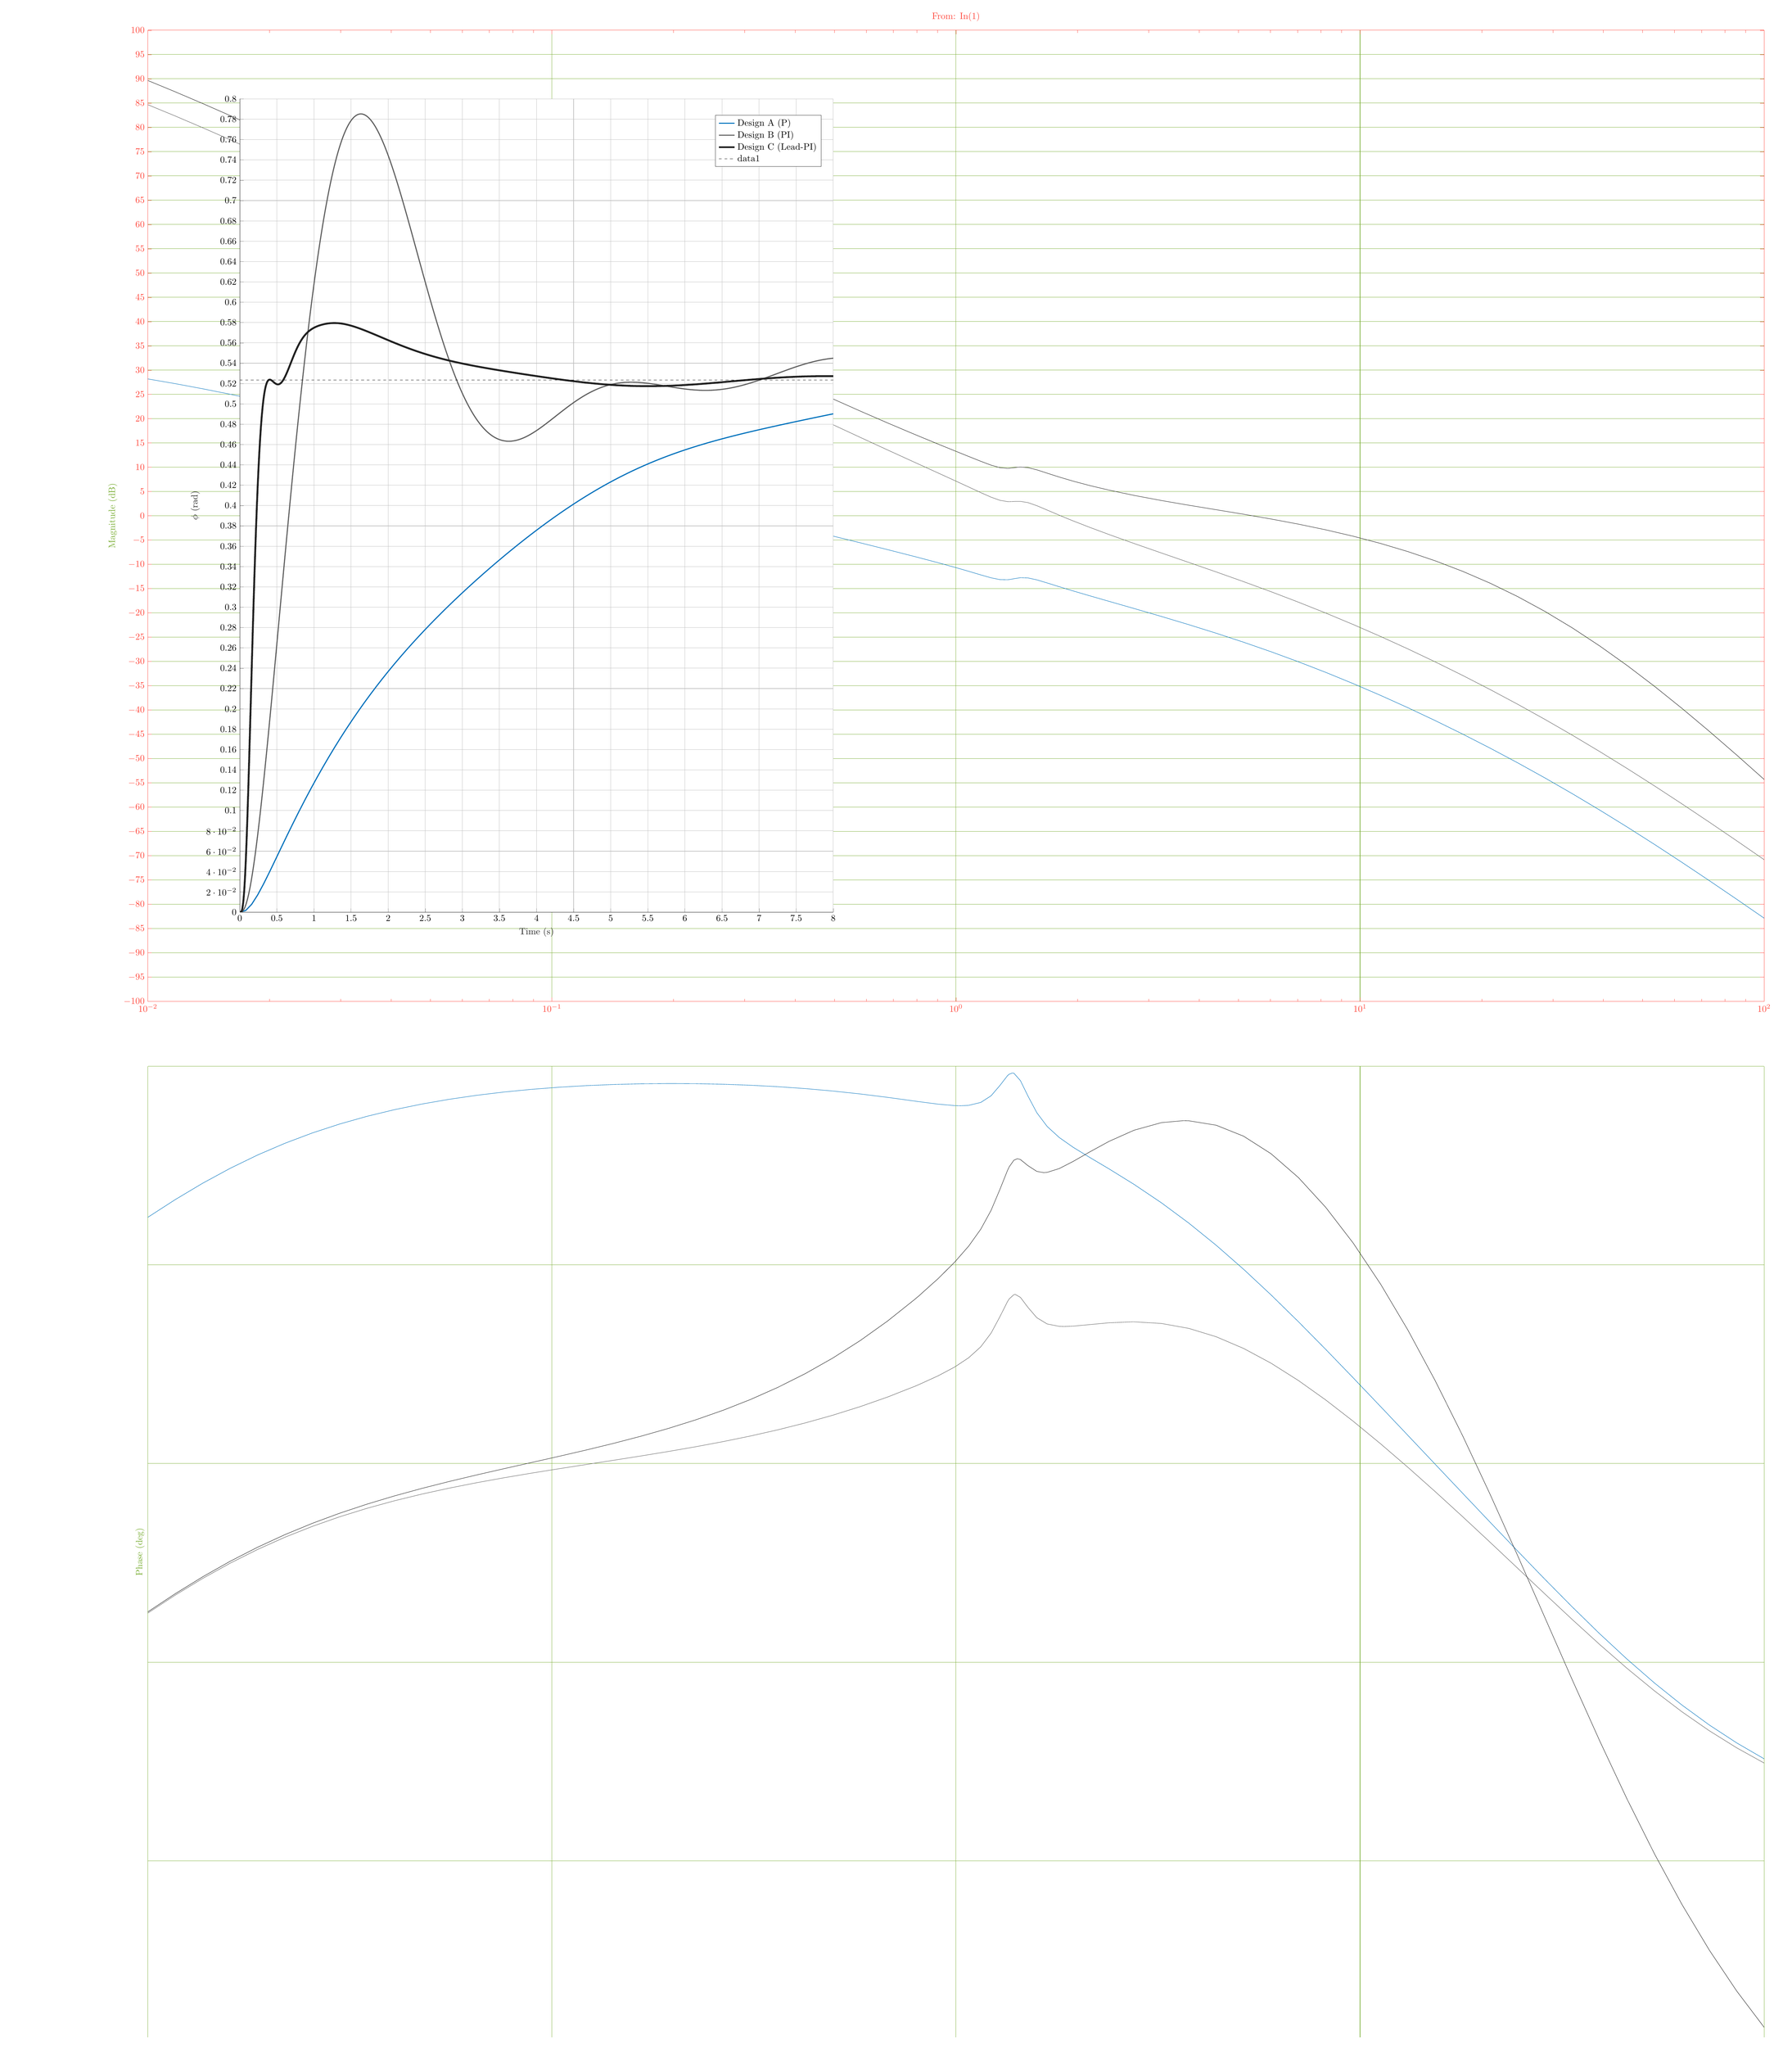
\begin{tikzpicture}

\begin{axis}[%
width=24.303in,
height=14.598in,
at={(2.085in,-15.264in)},
scale only axis,
unbounded coords=jump,
separate axis lines,
every outer x axis line/.append style={mycolor5},
every x tick label/.append style={font=\color{mycolor5}},
every x tick/.append style={mycolor5},
xmode=log,
xmin=0.01,
xmax=100,
xtick={0.01,0.1,1,10,100},
xticklabels={\empty},
xminorticks=true,
every outer y axis line/.append style={mycolor5},
every y tick label/.append style={font=\color{mycolor5}},
every y tick/.append style={mycolor5},
ymin=-310,
ymax=-90,
ytick={-315,-270,-225,-180,-135,-90},
yticklabels={\empty},
ylabel style={font=\color{mycolor6}},
ylabel={Phase (deg)},
axis line style={draw=none},
ticks=none,
xmajorgrids,
ymajorgrids,
grid style={mycolor6}
]
\addplot [color=mycolor1, line width=1.5pt, forget plot]
  table[row sep=crcr]{%
nan	-310\\
nan	-90\\
};
\addplot [color=mycolor1, line width=1.5pt, forget plot]
  table[row sep=crcr]{%
nan	-310\\
nan	-90\\
};
\addplot [color=mycolor1, line width=1.5pt, forget plot]
  table[row sep=crcr]{%
nan	-310\\
nan	-90\\
};
\addplot [color=mycolor1, line width=1.5pt, forget plot]
  table[row sep=crcr]{%
nan	-310\\
nan	-90\\
};
\addplot [color=mycolor1, line width=1.5pt, forget plot]
  table[row sep=crcr]{%
nan	-310\\
nan	-90\\
};
\addplot [color=mycolor1, line width=1.5pt, forget plot]
  table[row sep=crcr]{%
nan	-310\\
nan	-90\\
};
\addplot [color=mycolor2, forget plot]
  table[row sep=crcr]{%
-100	-246.889180911204\\
-85.5467253556568	-243.285025360282\\
-73.1824221907617	-239.226018127396\\
-62.6051657201482	-234.703214781408\\
-53.556669177069	-229.726862372165\\
-45.8159766905449	-224.329486840945\\
-39.1940677484722	-218.565423902727\\
-33.5292414924956	-212.505647449648\\
-28.6831681334201	-206.228345557223\\
-24.5375110663982	-199.807648916422\\
-20.9910372010855	-193.304071099349\\
-17.9571449437164	-186.759769109756\\
-15.3617494667183	-180.199942284595\\
-13.1414736261176	-173.639595598737\\
-11.2421003506209	-167.093379281429\\
-9.61724871115296	-160.585511616889\\
-8.22724134170047	-154.156768672561\\
-7.03813555493155	-147.86617444521\\
-6.02089449333613	-141.786473247687\\
-5.15067807616812	-135.994505799144\\
-4.40623642777357	-130.559364920055\\
-3.76939097538836	-125.531530061385\\
-3.22459054529639	-120.934440414497\\
-2.75853161762918	-116.755778212185\\
-2.39237635077625	-113.251005292419\\
-2.14399148550879	-110.661458933364\\
-1.95196026166226	-108.377130614364\\
-1.80130128659818	-106.140061807877\\
-1.68160667044661	-103.639294238503\\
-1.58548448116874	-100.534832319269\\
-1.50757886072228	-96.769102124804\\
-1.44393831174424	-93.2646549712019\\
-1.39159923312489	-91.5922210080171\\
-1.37957330551108	-91.5262736881954\\
-1.35500109262074	-91.7876340630653\\
-1.34115731252706	-92.1379646571659\\
-1.28454204027906	-94.3523862545132\\
-1.22142376581715	-96.6903547713756\\
-1.15160605608174	-98.199375732972\\
-1.07508301917166	-98.8555795953017\\
-1.02608589786395	-98.9451321714001\\
-0.992104431462472	-98.9109068480215\\
-0.903244457229836	-98.5837193879302\\
-0.809466464172925	-98.0197445405566\\
-0.791234261898132	-97.8945776391606\\
-0.676875000945854	-97.0440219906756\\
-0.579044398060249	-96.2708618941614\\
-0.495353520895917	-95.608586292651\\
-0.423758716060406	-95.0622839833508\\
-0.362511704998853	-94.6284105572593\\
-0.310116892657478	-94.3012933546563\\
-0.26529484644319	-94.0755681319155\\
-0.226951053669467	-93.9471739290603\\
-0.19863774351497	-93.9127762453995\\
-0.194149194574388	-93.9137881469958\\
-0.166088278262772	-93.9750368993961\\
-0.142083083253392	-94.1326204867298\\
-0.121547425007629	-94.3904162693414\\
-0.103979841848149	-94.7545870511402\\
-0.0889513497310823	-95.2337058549708\\
-0.0760949668545988	-95.8388970371921\\
-0.0650967523045817	-96.5839840191222\\
-0.0556881399094527	-97.4856224467099\\
-0.0476393801040134	-98.563381847757\\
-0.0407539296587178	-99.8397164783135\\
-0.0348636522767809	-101.339734989757\\
-0.0298247128621689	-103.090638142685\\
-0.0255140652003129	-105.120647283391\\
-0.0218264472839749	-107.457205505077\\
-0.0186718109129192	-110.124225645052\\
-0.0159731228006025	-113.138233788224\\
-0.0136644834929533	-116.503482032826\\
-0.0116895181649858	-120.206537008406\\
-0.01	-124.211461633229\\
0.01	-124.211461633229\\
0.0116895181649858	-120.206537008406\\
0.0136644834929533	-116.503482032826\\
0.0159731228006025	-113.138233788224\\
0.0186718109129192	-110.124225645052\\
0.0218264472839749	-107.457205505077\\
0.0255140652003129	-105.120647283391\\
0.0298247128621689	-103.090638142685\\
0.0348636522767809	-101.339734989757\\
0.0407539296587178	-99.8397164783135\\
0.0476393801040134	-98.563381847757\\
0.0556881399094527	-97.4856224467099\\
0.0650967523045817	-96.5839840191222\\
0.0760949668545988	-95.8388970371921\\
0.0889513497310823	-95.2337058549708\\
0.103979841848149	-94.7545870511402\\
0.121547425007629	-94.3904162693414\\
0.142083083253392	-94.1326204867298\\
0.166088278262772	-93.9750368993961\\
0.194149194574388	-93.9137881469958\\
0.19863774351497	-93.9127762453995\\
0.226951053669467	-93.9471739290603\\
0.26529484644319	-94.0755681319155\\
0.310116892657478	-94.3012933546563\\
0.362511704998853	-94.6284105572593\\
0.423758716060406	-95.0622839833508\\
0.495353520895917	-95.608586292651\\
0.579044398060249	-96.2708618941614\\
0.676875000945854	-97.0440219906756\\
0.791234261898132	-97.8945776391606\\
0.809466464172925	-98.0197445405566\\
0.903244457229836	-98.5837193879302\\
0.992104431462472	-98.9109068480215\\
1.02608589786395	-98.9451321714001\\
1.07508301917166	-98.8555795953017\\
1.15160605608174	-98.199375732972\\
1.22142376581715	-96.6903547713756\\
1.28454204027906	-94.3523862545132\\
1.34115731252706	-92.1379646571659\\
1.35500109262074	-91.7876340630653\\
1.37957330551108	-91.5262736881954\\
1.39159923312489	-91.5922210080171\\
1.44393831174424	-93.2646549712019\\
1.50757886072228	-96.769102124804\\
1.58548448116874	-100.534832319269\\
1.68160667044661	-103.639294238503\\
1.80130128659818	-106.140061807877\\
1.95196026166226	-108.377130614364\\
2.14399148550879	-110.661458933364\\
2.39237635077625	-113.251005292419\\
2.75853161762918	-116.755778212185\\
3.22459054529639	-120.934440414497\\
3.76939097538836	-125.531530061385\\
4.40623642777357	-130.559364920055\\
5.15067807616812	-135.994505799144\\
6.02089449333613	-141.786473247687\\
7.03813555493155	-147.86617444521\\
8.22724134170047	-154.156768672561\\
9.61724871115296	-160.585511616889\\
11.2421003506209	-167.093379281429\\
13.1414736261176	-173.639595598737\\
15.3617494667183	-180.199942284595\\
17.9571449437164	-186.759769109756\\
20.9910372010855	-193.304071099349\\
24.5375110663982	-199.807648916422\\
28.6831681334201	-206.228345557223\\
33.5292414924956	-212.505647449648\\
39.1940677484722	-218.565423902727\\
45.8159766905449	-224.329486840945\\
53.556669177069	-229.726862372165\\
62.6051657201482	-234.703214781408\\
73.1824221907617	-239.226018127396\\
85.5467253556568	-243.285025360282\\
100	-246.889180911204\\
};
\addplot [color=mycolor3, forget plot]
  table[row sep=crcr]{%
-100	-247.844022165077\\
-85.5467253556568	-244.401150918016\\
-73.1824221907617	-240.530654659328\\
-62.6051657201482	-236.228175460905\\
-53.556669177069	-231.509313726681\\
-45.8159766905449	-226.412840371808\\
-39.1940677484722	-221.000370708157\\
-33.5292414924956	-215.351355486638\\
-28.6831681334201	-209.553839836064\\
-24.5375110663982	-203.693394153369\\
-20.9910372010855	-197.843773058103\\
-17.9571449437164	-192.062403309568\\
-15.3617494667183	-186.392004283254\\
-13.1414736261176	-180.867541709938\\
-11.2421003506209	-175.526184687712\\
-9.61724871115296	-170.41720675631\\
-8.22724134170047	-165.608715231929\\
-7.03813555493155	-161.188700163982\\
-6.02089449333613	-157.259295932938\\
-5.15067807616812	-153.925152634343\\
-4.40623642777357	-151.278577201967\\
-3.76939097538836	-149.384535197443\\
-3.22459054529639	-148.267141525726\\
-2.75853161762918	-147.895569492525\\
-2.74056502950711	-147.89500804135\\
-2.39237635077625	-148.114288382141\\
-2.14399148550879	-148.521749003766\\
-1.95196026166226	-148.869239370193\\
-1.85257528069098	-148.950654769454\\
-1.80130128659818	-148.916822245379\\
-1.68160667044661	-148.38364202748\\
-1.58548448116874	-146.964787633674\\
-1.50757886072228	-144.638268792743\\
-1.44393831174424	-142.360209541983\\
-1.40184847594141	-141.68449658122\\
-1.39159923312489	-141.73170548601\\
-1.35500109262074	-142.676500644128\\
-1.34115731252706	-143.314526313809\\
-1.28454204027906	-146.730038317009\\
-1.22142376581715	-150.454370836478\\
-1.15160605608174	-153.556312962162\\
-1.07508301917166	-156.031548071502\\
-0.992104431462472	-158.14714812826\\
-0.903244457229835	-160.128388303385\\
-0.809466464172925	-162.114831642027\\
-0.791234261898132	-162.498989239996\\
-0.676875000945854	-164.940721296655\\
-0.579044398060249	-167.112273025233\\
-0.495353520895917	-169.055999394208\\
-0.423758716060406	-170.796806127763\\
-0.362511704998853	-172.35730598744\\
-0.310116892657478	-173.760801361555\\
-0.26529484644319	-175.03127965858\\
-0.226951053669467	-176.192864638837\\
-0.194149194574388	-177.269376951094\\
-0.166088278262772	-178.28413109963\\
-0.142083083253392	-179.259945206368\\
-0.121547425007629	-180.219307895183\\
-0.103979841848149	-181.184650294407\\
-0.0889513497310823	-182.178682189258\\
-0.0760949668545988	-183.224760204338\\
-0.0650967523045817	-184.347259454388\\
-0.0556881399094527	-185.571917170166\\
-0.0476393801040134	-186.926106397168\\
-0.0407539296587178	-188.438978708353\\
-0.0348636522767809	-190.141385676571\\
-0.0298247128621689	-192.065449460327\\
-0.0255140652003129	-194.243606837572\\
-0.0218264472839749	-196.706910408745\\
-0.0186718109129192	-199.482362920662\\
-0.0159731228006025	-202.589135086229\\
-0.0136644834929533	-206.033742217686\\
-0.0116895181649858	-209.80468756436\\
-0.01	-213.867691081358\\
0.01	-213.867691081358\\
0.0116895181649858	-209.80468756436\\
0.0136644834929533	-206.033742217686\\
0.0159731228006025	-202.589135086229\\
0.0186718109129192	-199.482362920662\\
0.0218264472839749	-196.706910408745\\
0.0255140652003129	-194.243606837572\\
0.0298247128621689	-192.065449460327\\
0.0348636522767809	-190.141385676571\\
0.0407539296587178	-188.438978708353\\
0.0476393801040134	-186.926106397168\\
0.0556881399094527	-185.571917170166\\
0.0650967523045817	-184.347259454388\\
0.0760949668545988	-183.224760204338\\
0.0889513497310823	-182.178682189258\\
0.103979841848149	-181.184650294407\\
0.121547425007629	-180.219307895183\\
0.142083083253392	-179.259945206368\\
0.166088278262772	-178.28413109963\\
0.194149194574388	-177.269376951094\\
0.226951053669467	-176.192864638837\\
0.26529484644319	-175.03127965858\\
0.310116892657478	-173.760801361555\\
0.362511704998853	-172.35730598744\\
0.423758716060406	-170.796806127763\\
0.495353520895917	-169.055999394208\\
0.579044398060249	-167.112273025233\\
0.676875000945854	-164.940721296655\\
0.791234261898132	-162.498989239996\\
0.809466464172925	-162.114831642027\\
0.903244457229835	-160.128388303385\\
0.992104431462472	-158.14714812826\\
1.07508301917166	-156.031548071502\\
1.15160605608174	-153.556312962162\\
1.22142376581715	-150.454370836478\\
1.28454204027906	-146.730038317009\\
1.34115731252706	-143.314526313809\\
1.35500109262074	-142.676500644128\\
1.39159923312489	-141.73170548601\\
1.40184847594141	-141.68449658122\\
1.44393831174424	-142.360209541983\\
1.50757886072228	-144.638268792743\\
1.58548448116874	-146.964787633674\\
1.68160667044661	-148.38364202748\\
1.80130128659818	-148.916822245379\\
1.85257528069098	-148.950654769454\\
1.95196026166226	-148.869239370193\\
2.14399148550879	-148.521749003766\\
2.39237635077625	-148.114288382141\\
2.74056502950711	-147.89500804135\\
2.75853161762918	-147.895569492525\\
3.22459054529639	-148.267141525726\\
3.76939097538836	-149.384535197443\\
4.40623642777357	-151.278577201967\\
5.15067807616812	-153.925152634343\\
6.02089449333613	-157.259295932938\\
7.03813555493155	-161.188700163982\\
8.22724134170047	-165.608715231929\\
9.61724871115296	-170.41720675631\\
11.2421003506209	-175.526184687712\\
13.1414736261176	-180.867541709938\\
15.3617494667183	-186.392004283254\\
17.9571449437164	-192.062403309568\\
20.9910372010855	-197.843773058103\\
24.5375110663982	-203.693394153369\\
28.6831681334201	-209.553839836064\\
33.5292414924956	-215.351355486638\\
39.1940677484722	-221.000370708157\\
45.8159766905449	-226.412840371808\\
53.556669177069	-231.509313726681\\
62.6051657201482	-236.228175460905\\
73.1824221907617	-240.530654659328\\
85.5467253556568	-244.401150918016\\
100	-247.844022165077\\
};
\addplot [color=mycolor4, forget plot]
  table[row sep=crcr]{%
-100	-307.705612515528\\
-85.5467253556568	-299.49357313132\\
-73.1824221907617	-290.222250686956\\
-62.6051657201482	-279.865466862981\\
-53.556669177069	-268.446325544774\\
-45.8159766905449	-256.05127467557\\
-39.1940677484722	-242.83841727364\\
-33.5292414924956	-229.035327593578\\
-28.6831681334201	-214.923583414785\\
-24.5375110663982	-200.811508565587\\
-20.9910372010855	-187.001527403424\\
-17.9571449437164	-173.761264342587\\
-15.3617494667183	-161.306219196459\\
-13.1414736261176	-149.797186201434\\
-11.2421003506209	-139.350182739166\\
-9.61724871115296	-130.052981963511\\
-8.22724134170047	-121.981311671458\\
-7.03813555493155	-115.208996488229\\
-6.02089449333613	-109.808973938962\\
-5.15067807616812	-105.845320700636\\
-4.40623642777357	-103.359107970527\\
-3.76939097538836	-102.35202868948\\
-3.65537477663796	-102.32454484816\\
-3.22459054529639	-102.770815965975\\
-2.75853161762918	-104.492064124813\\
-2.39237635077625	-107.015608647208\\
-2.14399148550879	-109.397305851084\\
-1.95196026166226	-111.538657944906\\
-1.80130128659818	-113.177340519737\\
-1.68160667044661	-114.034278392502\\
-1.64845285105767	-114.093307704997\\
-1.58548448116874	-113.81840123128\\
-1.50757886072228	-112.526639439479\\
-1.44393831174424	-111.135285293291\\
-1.41957163236147	-110.941268701905\\
-1.39159923312488	-111.264874367195\\
-1.35500109262074	-112.755630213267\\
-1.34115731252706	-113.603632838799\\
-1.28454204027905	-117.897951557933\\
-1.22142376581715	-122.640843413019\\
-1.15160605608174	-126.918366951544\\
-1.07508301917166	-130.742619532461\\
-0.992104431462468	-134.394261625374\\
-0.903244457229831	-138.106456003623\\
-0.809466464172921	-142.017122482169\\
-0.791234261898132	-142.78700744201\\
-0.676875000945854	-147.733475079152\\
-0.579044398060249	-152.161442038429\\
-0.495353520895917	-156.113938512481\\
-0.423758716060406	-159.62618062507\\
-0.362511704998853	-162.737244082207\\
-0.310116892657478	-165.490193409108\\
-0.26529484644319	-167.929964594832\\
-0.226951053669467	-170.101387852329\\
-0.194149194574388	-172.047870136045\\
-0.166088278262772	-173.810717134526\\
-0.142083083253392	-175.428942120708\\
-0.121547425007629	-176.939406269229\\
-0.103979841848149	-178.377167221252\\
-0.0889513497310823	-179.775946945431\\
-0.0760949668545988	-181.168655985838\\
-0.0650967523045817	-182.587926706697\\
-0.0556881399094527	-184.066613170455\\
-0.0476393801040134	-185.638209983758\\
-0.0407539296587178	-187.337126458381\\
-0.0348636522767809	-189.198725133757\\
-0.0298247128621689	-191.258995395308\\
-0.0255140652003129	-193.553687473955\\
-0.0218264472839749	-196.116691758477\\
-0.0186718109129192	-198.977440659127\\
-0.0159731228006025	-202.157184656861\\
-0.0136644834929533	-205.664219033102\\
-0.0116895181649858	-209.48857024082\\
-0.01	-213.597261597978\\
0.01	-213.597261597978\\
0.0116895181649858	-209.48857024082\\
0.0136644834929533	-205.664219033102\\
0.0159731228006025	-202.157184656861\\
0.0186718109129192	-198.977440659127\\
0.0218264472839749	-196.116691758477\\
0.0255140652003129	-193.553687473955\\
0.0298247128621689	-191.258995395308\\
0.0348636522767809	-189.198725133757\\
0.0407539296587178	-187.337126458381\\
0.0476393801040134	-185.638209983758\\
0.0556881399094527	-184.066613170455\\
0.0650967523045817	-182.587926706697\\
0.0760949668545988	-181.168655985838\\
0.0889513497310823	-179.775946945431\\
0.103979841848149	-178.377167221252\\
0.121547425007629	-176.939406269229\\
0.142083083253392	-175.428942120708\\
0.166088278262772	-173.810717134526\\
0.194149194574388	-172.047870136045\\
0.226951053669467	-170.101387852329\\
0.26529484644319	-167.929964594832\\
0.310116892657478	-165.490193409108\\
0.362511704998853	-162.737244082207\\
0.423758716060406	-159.62618062507\\
0.495353520895917	-156.113938512481\\
0.579044398060249	-152.161442038429\\
0.676875000945854	-147.733475079152\\
0.791234261898132	-142.78700744201\\
0.809466464172921	-142.017122482169\\
0.903244457229831	-138.106456003623\\
0.992104431462468	-134.394261625374\\
1.07508301917166	-130.742619532461\\
1.15160605608174	-126.918366951544\\
1.22142376581715	-122.640843413019\\
1.28454204027905	-117.897951557933\\
1.34115731252706	-113.603632838799\\
1.35500109262074	-112.755630213267\\
1.39159923312488	-111.264874367195\\
1.41957163236147	-110.941268701905\\
1.44393831174424	-111.135285293291\\
1.50757886072228	-112.526639439479\\
1.58548448116874	-113.81840123128\\
1.64845285105767	-114.093307704997\\
1.68160667044661	-114.034278392502\\
1.80130128659818	-113.177340519737\\
1.95196026166226	-111.538657944906\\
2.14399148550879	-109.397305851084\\
2.39237635077625	-107.015608647208\\
2.75853161762918	-104.492064124813\\
3.22459054529639	-102.770815965975\\
3.65537477663796	-102.32454484816\\
3.76939097538836	-102.35202868948\\
4.40623642777357	-103.359107970527\\
5.15067807616812	-105.845320700636\\
6.02089449333613	-109.808973938962\\
7.03813555493155	-115.208996488229\\
8.22724134170047	-121.981311671458\\
9.61724871115296	-130.052981963511\\
11.2421003506209	-139.350182739166\\
13.1414736261176	-149.797186201434\\
15.3617494667183	-161.306219196459\\
17.9571449437164	-173.761264342587\\
20.9910372010855	-187.001527403424\\
24.5375110663982	-200.811508565587\\
28.6831681334201	-214.923583414785\\
33.5292414924956	-229.035327593578\\
39.1940677484722	-242.83841727364\\
45.8159766905449	-256.05127467557\\
53.556669177069	-268.446325544774\\
62.6051657201482	-279.865466862981\\
73.1824221907617	-290.222250686956\\
85.5467253556568	-299.49357313132\\
100	-307.705612515528\\
};
\end{axis}

\begin{axis}[%
width=24.303in,
height=14.598in,
at={(2.085in,0.309in)},
scale only axis,
unbounded coords=jump,
separate axis lines,
every outer x axis line/.append style={mycolor5},
every x tick label/.append style={font=\color{mycolor5}},
every x tick/.append style={mycolor5},
xmode=log,
xmin=0.01,
xmax=100,
xminorticks=true,
every outer y axis line/.append style={mycolor5},
every y tick label/.append style={font=\color{mycolor5}},
every y tick/.append style={mycolor5},
ymin=-100,
ymax=100,
ylabel style={font=\color{mycolor6}},
ylabel={Magnitude (dB)},
axis background/.style={fill=white},
title style={font=\color{mycolor5}},
title={From: In(1)},
xmajorgrids,
ymajorgrids,
grid style={mycolor6},
legend style={legend cell align=left, align=left}
]
\addplot [color=mycolor1, line width=1.5pt, forget plot]
  table[row sep=crcr]{%
nan	-100\\
nan	100\\
};
\addplot [color=mycolor1, line width=1.5pt, forget plot]
  table[row sep=crcr]{%
nan	-100\\
nan	100\\
};
\addplot [color=mycolor1, line width=1.5pt, forget plot]
  table[row sep=crcr]{%
nan	-100\\
nan	100\\
};
\addplot [color=mycolor1, line width=1.5pt, forget plot]
  table[row sep=crcr]{%
nan	-100\\
nan	100\\
};
\addplot [color=mycolor1, line width=1.5pt, forget plot]
  table[row sep=crcr]{%
nan	-100\\
nan	100\\
};
\addplot [color=mycolor1, line width=1.5pt, forget plot]
  table[row sep=crcr]{%
nan	-100\\
nan	100\\
};
\addplot [color=mycolor2, forget plot]
  table[row sep=crcr]{%
-100	-82.8564115228265\\
-85.5467253556568	-78.9659407069561\\
-73.1824221907617	-75.1301356443448\\
-62.6051657201482	-71.3619914587826\\
-53.556669177069	-67.6753181292187\\
-45.8159766905449	-64.0836372377637\\
-39.1940677484722	-60.5988043187767\\
-33.5292414924956	-57.2296888986709\\
-28.6831681334201	-53.9813520763124\\
-24.5375110663982	-50.8550693132923\\
-20.9910372010855	-47.8492517954211\\
-17.9571449437164	-44.9609716328349\\
-15.3617494667183	-42.1875829325174\\
-13.1414736261176	-39.5279321474121\\
-11.2421003506209	-36.9828108618545\\
-9.61724871115296	-34.5545258546251\\
-8.22724134170047	-32.2456925077664\\
-7.03813555493155	-30.0575792346795\\
-6.02089449333613	-27.988492678904\\
-5.15067807616812	-26.0326983606921\\
-4.40623642777357	-24.180151660679\\
-3.76939097538836	-22.4169259096048\\
-3.22459054529639	-20.7258146085798\\
-2.75853161762918	-19.0861937516305\\
-2.39237635077625	-17.613064012835\\
-2.14399148550879	-16.4751451020785\\
-1.95196026166226	-15.4811376469751\\
-1.80130128659818	-14.6016814614468\\
-1.68160667044661	-13.8271722742804\\
-1.58548448116874	-13.1897891659639\\
-1.50757886072228	-12.7917033992952\\
-1.44393831174424	-12.7445777084054\\
-1.39159923312489	-12.9533927404257\\
-1.37957330551108	-13.0144073694213\\
-1.35500109262074	-13.1237322599761\\
-1.34115731252706	-13.1666990111837\\
-1.28454204027906	-13.136708798086\\
-1.22142376581715	-12.7674170245774\\
-1.15160605608174	-12.1635770979372\\
-1.07508301917166	-11.4261318795501\\
-1.02608589786395	-10.9373181368381\\
-0.992104431462472	-10.5921200383121\\
-0.903244457229836	-9.66012224951349\\
-0.809466464172925	-8.61232073021029\\
-0.791234261898132	-8.39855611845482\\
-0.676875000945854	-6.95895338924452\\
-0.579044398060249	-5.54908099707682\\
-0.495353520895917	-4.15701600614817\\
-0.423758716060406	-2.77630414200438\\
-0.362511704998853	-1.40316998055083\\
-0.310116892657478	-0.0352789939812091\\
-0.26529484644319	1.3288628577063\\
-0.226951053669467	2.69022368268803\\
-0.19863774351497	3.8505373313111\\
-0.194149194574388	4.04942000830995\\
-0.166088278262772	5.40681607737917\\
-0.142083083253392	6.76257912570526\\
-0.121547425007629	8.11670598082094\\
-0.103979841848149	9.46902845023783\\
-0.0889513497310823	10.8192006064442\\
-0.0760949668545988	12.1666683527655\\
-0.0650967523045817	13.5106197271157\\
-0.0556881399094527	14.849912920974\\
-0.0476393801040134	16.1829779157624\\
-0.0407539296587178	17.5076872081577\\
-0.0348636522767809	18.8211919080954\\
-0.0298247128621689	20.1197226404488\\
-0.0255140652003129	21.3983618718884\\
-0.0218264472839749	22.6508077621465\\
-0.0186718109129192	23.8691714892402\\
-0.0159731228006025	25.0438801721897\\
-0.0136644834929533	26.1637899883587\\
-0.0116895181649858	27.2166319352287\\
-0.01	28.1898866184175\\
0.01	28.1898866184175\\
0.0116895181649858	27.2166319352287\\
0.0136644834929533	26.1637899883587\\
0.0159731228006025	25.0438801721897\\
0.0186718109129192	23.8691714892402\\
0.0218264472839749	22.6508077621465\\
0.0255140652003129	21.3983618718884\\
0.0298247128621689	20.1197226404488\\
0.0348636522767809	18.8211919080954\\
0.0407539296587178	17.5076872081577\\
0.0476393801040134	16.1829779157624\\
0.0556881399094527	14.849912920974\\
0.0650967523045817	13.5106197271157\\
0.0760949668545988	12.1666683527655\\
0.0889513497310823	10.8192006064442\\
0.103979841848149	9.46902845023783\\
0.121547425007629	8.11670598082094\\
0.142083083253392	6.76257912570526\\
0.166088278262772	5.40681607737917\\
0.194149194574388	4.04942000830995\\
0.19863774351497	3.8505373313111\\
0.226951053669467	2.69022368268803\\
0.26529484644319	1.3288628577063\\
0.310116892657478	-0.0352789939812091\\
0.362511704998853	-1.40316998055083\\
0.423758716060406	-2.77630414200438\\
0.495353520895917	-4.15701600614817\\
0.579044398060249	-5.54908099707682\\
0.676875000945854	-6.95895338924452\\
0.791234261898132	-8.39855611845482\\
0.809466464172925	-8.61232073021029\\
0.903244457229836	-9.66012224951349\\
0.992104431462472	-10.5921200383121\\
1.02608589786395	-10.9373181368381\\
1.07508301917166	-11.4261318795501\\
1.15160605608174	-12.1635770979372\\
1.22142376581715	-12.7674170245774\\
1.28454204027906	-13.136708798086\\
1.34115731252706	-13.1666990111837\\
1.35500109262074	-13.1237322599761\\
1.37957330551108	-13.0144073694213\\
1.39159923312489	-12.9533927404257\\
1.44393831174424	-12.7445777084054\\
1.50757886072228	-12.7917033992952\\
1.58548448116874	-13.1897891659639\\
1.68160667044661	-13.8271722742804\\
1.80130128659818	-14.6016814614468\\
1.95196026166226	-15.4811376469751\\
2.14399148550879	-16.4751451020785\\
2.39237635077625	-17.613064012835\\
2.75853161762918	-19.0861937516305\\
3.22459054529639	-20.7258146085798\\
3.76939097538836	-22.4169259096048\\
4.40623642777357	-24.180151660679\\
5.15067807616812	-26.0326983606921\\
6.02089449333613	-27.988492678904\\
7.03813555493155	-30.0575792346795\\
8.22724134170047	-32.2456925077664\\
9.61724871115296	-34.5545258546251\\
11.2421003506209	-36.9828108618545\\
13.1414736261176	-39.5279321474121\\
15.3617494667183	-42.1875829325174\\
17.9571449437164	-44.9609716328349\\
20.9910372010855	-47.8492517954211\\
24.5375110663982	-50.8550693132923\\
28.6831681334201	-53.9813520763124\\
33.5292414924956	-57.2296888986709\\
39.1940677484722	-60.5988043187767\\
45.8159766905449	-64.0836372377637\\
53.556669177069	-67.6753181292187\\
62.6051657201482	-71.3619914587826\\
73.1824221907617	-75.1301356443448\\
85.5467253556568	-78.9659407069561\\
100	-82.8564115228265\\
};
\addplot [color=mycolor3, forget plot]
  table[row sep=crcr]{%
-100	-70.8140054902273\\
-85.5467253556568	-66.9230927460066\\
-73.1824221907617	-63.0866838838288\\
-62.6051657201482	-59.3177147730479\\
-53.556669177069	-55.6299144790614\\
-45.8159766905449	-52.0366941215995\\
-39.1940677484722	-48.5497584837392\\
-33.5292414924956	-45.1777714519415\\
-28.6831681334201	-41.9255137879252\\
-24.5375110663982	-38.7938791140154\\
-20.9910372010855	-35.7807591333704\\
-17.9571449437164	-32.8825203436149\\
-15.3617494667183	-30.0955605097463\\
-13.1414736261176	-27.4174337720344\\
-11.2421003506209	-24.8471924663312\\
-9.61724871115296	-22.3848154893441\\
-8.22724134170047	-20.0298257383473\\
-7.03813555493155	-17.7794249063143\\
-6.02089449333613	-15.6266447073038\\
-5.15067807616812	-13.5590341388741\\
-4.40623642777357	-11.558206883172\\
-3.76939097538836	-9.60021659976326\\
-3.22459054529639	-7.6563489061083\\
-2.75853161762918	-5.69353717563081\\
-2.74056502950711	-5.61041610052026\\
-2.39237635077625	-3.85363021279085\\
-2.14399148550879	-2.38109398928963\\
-1.95196026166226	-1.06186971514181\\
-1.85257528069098	-0.296176256325292\\
-1.80130128659818	0.125533381248428\\
-1.68160667044661	1.18574372242419\\
-1.58548448116874	2.08399061483029\\
-1.50757886072228	2.7173011387487\\
-1.44393831174424	2.97445591373086\\
-1.40184847594141	2.96585118634296\\
-1.39159923312489	2.95171976949777\\
-1.35500109262074	2.91926770730467\\
-1.34115731252706	2.93022274343795\\
-1.28454204027906	3.19143007283507\\
-1.22142376581715	3.84038209687377\\
-1.15160605608174	4.78359023691886\\
-1.07508301917166	5.93410918165409\\
-0.992104431462472	7.2721764542705\\
-0.903244457229835	8.8203030529825\\
-0.809466464172925	10.6216572885964\\
-0.791234261898132	10.9962199089151\\
-0.676875000945854	13.5720782548543\\
-0.579044398060249	16.1697706728742\\
-0.495353520895917	18.7904798466351\\
-0.423758716060406	21.4315489280576\\
-0.362511704998853	24.089313781745\\
-0.310116892657478	26.7602048398564\\
-0.26529484644319	29.4411289200136\\
-0.226951053669467	32.129545734644\\
-0.194149194574388	34.823419614668\\
-0.166088278262772	37.521127036082\\
-0.142083083253392	40.2213548605736\\
-0.121547425007629	42.9230025484338\\
-0.103979841848149	45.6250912364471\\
-0.0889513497310823	48.3266776249941\\
-0.0760949668545988	51.0267682331097\\
-0.0650967523045817	53.724228355501\\
-0.0556881399094527	56.4176793520599\\
-0.0476393801040134	59.1053775412709\\
-0.0407539296587178	61.7850681445505\\
-0.0348636522767809	64.4538090297516\\
-0.0298247128621689	67.107762531875\\
-0.0255140652003129	69.7419611129704\\
-0.0218264472839749	72.3500663229383\\
-0.0186718109129192	74.9241625396688\\
-0.0159731228006025	77.4546572648262\\
-0.0136644834929533	79.9303923169745\\
-0.0116895181649858	82.3390881842228\\
-0.01	84.6682177805032\\
0.01	84.6682177805032\\
0.0116895181649858	82.3390881842228\\
0.0136644834929533	79.9303923169745\\
0.0159731228006025	77.4546572648262\\
0.0186718109129192	74.9241625396688\\
0.0218264472839749	72.3500663229383\\
0.0255140652003129	69.7419611129704\\
0.0298247128621689	67.107762531875\\
0.0348636522767809	64.4538090297516\\
0.0407539296587178	61.7850681445505\\
0.0476393801040134	59.1053775412709\\
0.0556881399094527	56.4176793520599\\
0.0650967523045817	53.724228355501\\
0.0760949668545988	51.0267682331097\\
0.0889513497310823	48.3266776249941\\
0.103979841848149	45.6250912364471\\
0.121547425007629	42.9230025484338\\
0.142083083253392	40.2213548605736\\
0.166088278262772	37.521127036082\\
0.194149194574388	34.823419614668\\
0.226951053669467	32.129545734644\\
0.26529484644319	29.4411289200136\\
0.310116892657478	26.7602048398564\\
0.362511704998853	24.089313781745\\
0.423758716060406	21.4315489280576\\
0.495353520895917	18.7904798466351\\
0.579044398060249	16.1697706728742\\
0.676875000945854	13.5720782548543\\
0.791234261898132	10.9962199089151\\
0.809466464172925	10.6216572885964\\
0.903244457229835	8.8203030529825\\
0.992104431462472	7.2721764542705\\
1.07508301917166	5.93410918165409\\
1.15160605608174	4.78359023691886\\
1.22142376581715	3.84038209687377\\
1.28454204027906	3.19143007283507\\
1.34115731252706	2.93022274343795\\
1.35500109262074	2.91926770730467\\
1.39159923312489	2.95171976949777\\
1.40184847594141	2.96585118634296\\
1.44393831174424	2.97445591373086\\
1.50757886072228	2.7173011387487\\
1.58548448116874	2.08399061483029\\
1.68160667044661	1.18574372242419\\
1.80130128659818	0.125533381248428\\
1.85257528069098	-0.296176256325292\\
1.95196026166226	-1.06186971514181\\
2.14399148550879	-2.38109398928963\\
2.39237635077625	-3.85363021279085\\
2.74056502950711	-5.61041610052026\\
2.75853161762918	-5.69353717563081\\
3.22459054529639	-7.6563489061083\\
3.76939097538836	-9.60021659976326\\
4.40623642777357	-11.558206883172\\
5.15067807616812	-13.5590341388741\\
6.02089449333613	-15.6266447073038\\
7.03813555493155	-17.7794249063143\\
8.22724134170047	-20.0298257383473\\
9.61724871115296	-22.3848154893441\\
11.2421003506209	-24.8471924663312\\
13.1414736261176	-27.4174337720344\\
15.3617494667183	-30.0955605097463\\
17.9571449437164	-32.8825203436149\\
20.9910372010855	-35.7807591333704\\
24.5375110663982	-38.7938791140154\\
28.6831681334201	-41.9255137879252\\
33.5292414924956	-45.1777714519415\\
39.1940677484722	-48.5497584837392\\
45.8159766905449	-52.0366941215995\\
53.556669177069	-55.6299144790614\\
62.6051657201482	-59.3177147730479\\
73.1824221907617	-63.0866838838288\\
85.5467253556568	-66.9230927460066\\
100	-70.8140054902273\\
};
\addplot [color=mycolor4, forget plot]
  table[row sep=crcr]{%
-100	-54.2867053944414\\
-85.5467253556568	-49.2675546992761\\
-73.1824221907617	-44.3769448991568\\
-62.6051657201482	-39.6479991095864\\
-53.556669177069	-35.1175232883119\\
-45.8159766905449	-30.8237147279683\\
-39.1940677484722	-26.8027024781368\\
-33.5292414924956	-23.0843635741785\\
-28.6831681334201	-19.6883466311565\\
-24.5375110663982	-16.6214676561952\\
-20.9910372010855	-13.8773653761001\\
-17.9571449437164	-11.4385415869769\\
-15.3617494667183	-9.28003736952944\\
-13.1414736261176	-7.37347373701934\\
-11.2421003506209	-5.69023093501922\\
-9.61724871115296	-4.20302251825057\\
-8.22724134170047	-2.88574894408977\\
-7.03813555493155	-1.71205857942906\\
-6.02089449333613	-0.653377321696027\\
-5.15067807616812	0.322773336013201\\
-4.40623642777357	1.25357327935277\\
-3.76939097538836	2.18063428136023\\
-3.65537477663796	2.36643161056958\\
-3.22459054529639	3.14894927425122\\
-2.75853161762918	4.20585492374532\\
-2.39237635077625	5.28982932812777\\
-2.14399148550879	6.23041466916585\\
-1.95196026166226	7.13024008834051\\
-1.80130128659818	7.98537662523051\\
-1.68160667044661	8.78076029776561\\
-1.64845285105767	9.01702522094903\\
-1.58548448116874	9.46654727042516\\
-1.50757886072228	9.92827871747167\\
-1.44393831174424	10.0459791066089\\
-1.41957163236147	10.0011993725895\\
-1.39159923312488	9.90921404259926\\
-1.35500109262074	9.79746666199222\\
-1.34115731252706	9.77853452096572\\
-1.28454204027905	9.91821274746286\\
-1.22142376581715	10.4332070343182\\
-1.15160605608174	11.2305143760277\\
-1.07508301917166	12.2244470342025\\
-0.992104431462468	13.397483878872\\
-0.903244457229831	14.7755370707826\\
-0.809466464172921	16.4064035010969\\
-0.791234261898132	16.7490420859301\\
-0.676875000945854	19.1350699532444\\
-0.579044398060249	21.586579438075\\
-0.495353520895917	24.0959906572253\\
-0.423758716060406	26.6531017948454\\
-0.362511704998853	29.2479957631221\\
-0.310116892657478	31.8720748415943\\
-0.26529484644319	34.518296235587\\
-0.226951053669467	37.1810724225946\\
-0.194149194574388	39.8560484487805\\
-0.166088278262772	42.5398534808808\\
-0.142083083253392	45.2298679710696\\
-0.121547425007629	47.9240201206909\\
-0.103979841848149	50.6206119882382\\
-0.0889513497310823	53.318169537302\\
-0.0760949668545988	56.0153084483478\\
-0.0650967523045817	58.7106066788124\\
-0.0556881399094527	61.402474601781\\
-0.0476393801040134	64.0890137506831\\
-0.0407539296587178	66.7678558675023\\
-0.0348636522767809	69.4359756636229\\
-0.0298247128621689	72.0894745594103\\
-0.0255140652003129	74.7233404066266\\
-0.0218264472839749	77.3312020914091\\
-0.0186718109129192	79.9051200784722\\
-0.0159731228006025	82.4354843643938\\
-0.0136644834929533	84.9111239544962\\
-0.0116895181649858	87.3197499584572\\
-0.01	89.6488284261008\\
0.01	89.6488284261008\\
0.0116895181649858	87.3197499584572\\
0.0136644834929533	84.9111239544962\\
0.0159731228006025	82.4354843643938\\
0.0186718109129192	79.9051200784722\\
0.0218264472839749	77.3312020914091\\
0.0255140652003129	74.7233404066266\\
0.0298247128621689	72.0894745594103\\
0.0348636522767809	69.4359756636229\\
0.0407539296587178	66.7678558675023\\
0.0476393801040134	64.0890137506831\\
0.0556881399094527	61.402474601781\\
0.0650967523045817	58.7106066788124\\
0.0760949668545988	56.0153084483478\\
0.0889513497310823	53.318169537302\\
0.103979841848149	50.6206119882382\\
0.121547425007629	47.9240201206909\\
0.142083083253392	45.2298679710696\\
0.166088278262772	42.5398534808808\\
0.194149194574388	39.8560484487805\\
0.226951053669467	37.1810724225946\\
0.26529484644319	34.518296235587\\
0.310116892657478	31.8720748415943\\
0.362511704998853	29.2479957631221\\
0.423758716060406	26.6531017948454\\
0.495353520895917	24.0959906572253\\
0.579044398060249	21.586579438075\\
0.676875000945854	19.1350699532444\\
0.791234261898132	16.7490420859301\\
0.809466464172921	16.4064035010969\\
0.903244457229831	14.7755370707826\\
0.992104431462468	13.397483878872\\
1.07508301917166	12.2244470342025\\
1.15160605608174	11.2305143760277\\
1.22142376581715	10.4332070343182\\
1.28454204027905	9.91821274746286\\
1.34115731252706	9.77853452096572\\
1.35500109262074	9.79746666199222\\
1.39159923312488	9.90921404259926\\
1.41957163236147	10.0011993725895\\
1.44393831174424	10.0459791066089\\
1.50757886072228	9.92827871747167\\
1.58548448116874	9.46654727042516\\
1.64845285105767	9.01702522094903\\
1.68160667044661	8.78076029776561\\
1.80130128659818	7.98537662523051\\
1.95196026166226	7.13024008834051\\
2.14399148550879	6.23041466916585\\
2.39237635077625	5.28982932812777\\
2.75853161762918	4.20585492374532\\
3.22459054529639	3.14894927425122\\
3.65537477663796	2.36643161056958\\
3.76939097538836	2.18063428136023\\
4.40623642777357	1.25357327935277\\
5.15067807616812	0.322773336013201\\
6.02089449333613	-0.653377321696027\\
7.03813555493155	-1.71205857942906\\
8.22724134170047	-2.88574894408977\\
9.61724871115296	-4.20302251825057\\
11.2421003506209	-5.69023093501922\\
13.1414736261176	-7.37347373701934\\
15.3617494667183	-9.28003736952944\\
17.9571449437164	-11.4385415869769\\
20.9910372010855	-13.8773653761001\\
24.5375110663982	-16.6214676561952\\
28.6831681334201	-19.6883466311565\\
33.5292414924956	-23.0843635741785\\
39.1940677484722	-26.8027024781368\\
45.8159766905449	-30.8237147279683\\
53.556669177069	-35.1175232883119\\
62.6051657201482	-39.6479991095864\\
73.1824221907617	-44.3769448991568\\
85.5467253556568	-49.2675546992761\\
100	-54.2867053944414\\
};
\end{axis}

\begin{axis}[%
width=8.924in,
height=12.225in,
at={(3.467in,1.65in)},
scale only axis,
xmin=0,
xmax=8,
xlabel style={font=\color{white!15!black}},
xlabel={Time (s)},
ymin=0,
ymax=0.8,
ylabel style={font=\color{white!15!black}},
ylabel={$\phi$ (rad)},
axis background/.style={fill=white},
axis x line*=bottom,
axis y line*=left,
xmajorgrids,
ymajorgrids,
legend style={legend cell align=left, align=left, draw=white!15!black}
]
\addplot [color=mycolor2, line width=1.2pt]
  table[row sep=crcr]{%
0	0\\
0.08	0.00166633828000285\\
0.16	0.00772776129654752\\
0.24	0.0168444615185643\\
0.32	0.0276891050097778\\
0.4	0.0394269714927952\\
0.48	0.0515516153659193\\
0.56	0.0637577153340131\\
0.64	0.0758623290357947\\
0.72	0.0877570527554796\\
0.8	0.099379007704982\\
0.88	0.110693241256829\\
0.96	0.121682044447503\\
1.04	0.132338458245484\\
1.12	0.142662315272741\\
1.2	0.15265781500003\\
1.28	0.162332025367422\\
1.36	0.171693943252564\\
1.44	0.180753891419733\\
1.52	0.189523117637576\\
1.6	0.198013515048617\\
1.68	0.206237415248289\\
1.76	0.214207425154976\\
1.84	0.221936290639169\\
1.92	0.229436777069563\\
2	0.236721561270372\\
2.08	0.24380313198549\\
2.16	0.250693697489864\\
2.24	0.25740509988837\\
2.32	0.263948736147999\\
2.4	0.270335486172439\\
2.48	0.276575648342411\\
2.56	0.282678882967151\\
2.64	0.288654164057621\\
2.72	0.29450973976228\\
2.8	0.300253101715502\\
2.88	0.305890963446102\\
2.96	0.311429247884927\\
3.04	0.316873083900376\\
3.12	0.322226811682057\\
3.2	0.327493996687922\\
3.28	0.332677451770881\\
3.36	0.337779267008699\\
3.44	0.342800846676907\\
3.52	0.347742952729659\\
3.6	0.352605754088587\\
3.68	0.357388880985395\\
3.76	0.362091483560597\\
3.84	0.36671229388868\\
3.92	0.371249690579197\\
4	0.375701765093823\\
4.08	0.380066388921008\\
4.16	0.384341280762232\\
4.24	0.388524072906593\\
4.32	0.392612376002906\\
4.4	0.396603841479988\\
4.48	0.400496220915675\\
4.56	0.404287421712306\\
4.64	0.407975558500236\\
4.72	0.411558999760212\\
4.8	0.415036409229222\\
4.88	0.418406781731734\\
4.96	0.421669473157793\\
5.04	0.424824224390456\\
5.12	0.427871179066173\\
5.2	0.430810895132199\\
5.28	0.43364435024373\\
5.36	0.436372941119441\\
5.44	0.438998477046445\\
5.52	0.441523167793654\\
5.6	0.443949606255363\\
5.68	0.446280746203917\\
5.76	0.448519875581016\\
5.84	0.450670585801137\\
5.92	0.452736737577269\\
6	0.454722423808464\\
6.08	0.456631930090421\\
6.16	0.458469693424358\\
6.24	0.460240259705861\\
6.32	0.461948240574349\\
6.4	0.463598270195414\\
6.48	0.465194962533041\\
6.56	0.466742869646801\\
6.64	0.468246441521104\\
6.72	0.469709987900013\\
6.8	0.471137642562468\\
6.88	0.472533330429761\\
6.96	0.473900737850333\\
7.04	0.475243286357164\\
7.12	0.476564110140911\\
7.2	0.477866037428172\\
7.28	0.479151575899658\\
7.36	0.480422902228232\\
7.44	0.481681855762476\\
7.52	0.482929936328352\\
7.6	0.484168306070251\\
7.68	0.485397795203825\\
7.76	0.486618911507146\\
7.84	0.487831853334253\\
7.92	0.489036525896632\\
8	0.490232560523908\\
};
\addlegendentry{Design A (P)}

\addplot [color=mycolor3, line width=1.2pt]
  table[row sep=crcr]{%
0	0\\
0.0172043010752688	0.000115083225951973\\
0.0344086021505376	0.000789072739332498\\
0.0516129032258065	0.00230658169995276\\
0.0688172043010753	0.00478039242505776\\
0.0860215053763441	0.00823279363115475\\
0.103225806451613	0.0126396329948798\\
0.120430107526882	0.0179540766214954\\
0.137634408602151	0.024119332366227\\
0.154838709677419	0.0310753793678662\\
0.172043010752688	0.0387624497070007\\
0.189247311827957	0.047122756874218\\
0.206451612903226	0.0561012840557729\\
0.223655913978495	0.0656460739134277\\
0.240860215053763	0.0757082593077412\\
0.258064516129032	0.086241964324275\\
0.275268817204301	0.0972041450706343\\
0.29247311827957	0.108554407166129\\
0.309677419354839	0.120254819192911\\
0.326881720430108	0.132269731832901\\
0.344086021505376	0.144565607282145\\
0.361290322580645	0.157110860799657\\
0.378494623655914	0.169875714814531\\
0.395698924731183	0.182832065285971\\
0.412903225806452	0.195953359660795\\
0.43010752688172	0.209214485625453\\
0.447311827956989	0.222591669808464\\
0.464516129032258	0.236062385602737\\
0.481720430107527	0.249605269317347\\
0.498924731182796	0.263200043920063\\
0.516129032258065	0.276827449687388\\
0.533333333333333	0.290469181133915\\
0.550537634408602	0.304107829645527\\
0.567741935483871	0.317726831290335\\
0.58494623655914	0.331310419327057\\
0.602150537634409	0.344843580972735\\
0.619354838709677	0.358312018030344\\
0.636559139784946	0.371702111012281\\
0.653763440860215	0.385000886428116\\
0.670967741935484	0.398195986934535\\
0.688172043010753	0.411275644072427\\
0.705376344086021	0.424228653340703\\
0.72258064516129	0.43704435137895\\
0.739784946236559	0.449712595051531\\
0.756989247311828	0.462223742244486\\
0.774193548387097	0.474568634203697\\
0.791397849462366	0.486738579258354\\
0.808602150537634	0.498725337788016\\
0.825806451612903	0.510521108304559\\
0.843010752688172	0.522118514532117\\
0.860215053763441	0.533510593379006\\
0.87741935483871	0.544690783705426\\
0.894623655913979	0.555652915799794\\
0.911827956989247	0.566391201484767\\
0.929032258064516	0.576900224781497\\
0.946236559139785	0.58717493306755\\
0.963440860215054	0.597210628670126\\
0.980645161290323	0.607002960841938\\
0.997849462365591	0.616547918072305\\
1.01505376344086	0.625841820690774\\
1.03225806451613	0.63488131372487\\
1.0494623655914	0.643663359977594\\
1.06666666666667	0.652185233293818\\
1.08387096774194	0.660444511988056\\
1.1010752688172	0.668439072409078\\
1.11827956989247	0.676167082619548\\
1.13548387096774	0.683626996171378\\
1.15268817204301	0.690817545959732\\
1.16989247311828	0.697737738140716\\
1.18709677419355	0.704386846099627\\
1.20430107526882	0.71076440445838\\
1.22150537634409	0.716870203112286\\
1.23870967741935	0.722704281287737\\
1.25591397849462	0.728266921613702\\
1.27311827956989	0.733558644201042\\
1.29032258064516	0.738580200724757\\
1.30752688172043	0.743332568505226\\
1.3247311827957	0.747816944585369\\
1.34193548387097	0.752034739801445\\
1.35913978494624	0.755987572845932\\
1.37634408602151	0.759677264321546\\
1.39354838709677	0.763105830786061\\
1.41075268817204	0.766275478788095\\
1.42795698924731	0.76918859889451\\
1.44516129032258	0.771847759710459\\
1.46236559139785	0.774255701893529\\
1.47956989247312	0.776415332163714\\
1.49677419354839	0.778329717311279\\
1.51397849462366	0.780002078204807\\
1.53118279569892	0.781435783801966\\
1.54838709677419	0.782634345165709\\
1.56559139784946	0.783601409488805\\
1.58279569892473	0.784340754129737\\
1.6	0.784856280663106\\
1.61720430107527	0.785152008947815\\
1.63440860215054	0.785232071216349\\
1.65161290322581	0.785100706188555\\
1.66881720430108	0.78476225321336\\
1.68602150537634	0.784221146441895\\
1.70322580645161	0.783481909035525\\
1.72043010752688	0.782549147412261\\
1.73763440860215	0.781427545535052\\
1.75483870967742	0.780121859245421\\
1.77204301075269	0.778636910645879\\
1.78924731182796	0.776977582534525\\
1.80645161290323	0.775148812895193\\
1.82365591397849	0.773155589446437\\
1.84086021505376	0.771002944252609\\
1.85806451612903	0.768695948400218\\
1.8752688172043	0.766239706742648\\
1.89247311827957	0.763639352716308\\
1.90967741935484	0.760900043231121\\
1.92688172043011	0.758026953638249\\
1.94408602150538	0.755025272777806\\
1.96129032258065	0.751900198109257\\
1.97849462365591	0.748656930927073\\
1.99569892473118	0.745300671664138\\
2.01290322580645	0.741836615285286\\
2.03010752688172	0.738269946773261\\
2.04731182795699	0.734605836709254\\
2.06451612903226	0.730849436950111\\
2.08172043010753	0.727005876404156\\
2.0989247311828	0.723080256907482\\
2.11612903225806	0.719077649202463\\
2.13333333333333	0.715003089020102\\
2.1505376344086	0.71086157326774\\
2.16774193548387	0.70665805632354\\
2.18494623655914	0.702397446439033\\
2.20215053763441	0.69808460225091\\
2.21935483870968	0.693724329403144\\
2.23655913978495	0.689321377280387\\
2.25376344086022	0.68488043585351\\
2.27096774193548	0.680406132638018\\
2.28817204301075	0.67590302976597\\
2.30537634408602	0.671375621171942\\
2.32258064516129	0.666828329893435\\
2.33978494623656	0.662265505486049\\
2.35698924731183	0.657691421553633\\
2.3741935483871	0.6531102733935\\
2.39139784946237	0.648526175756725\\
2.40860215053763	0.64394316072342\\
2.4258064516129	0.63936517569279\\
2.44301075268817	0.634796081487672\\
2.46021505376344	0.630239650573177\\
2.47741935483871	0.625699565388937\\
2.49462365591398	0.6211794167944\\
2.51182795698925	0.616682702626496\\
2.52903225806452	0.612212826368923\\
2.54623655913979	0.60777309593222\\
2.56344086021505	0.603366722543712\\
2.58064516129032	0.598996819746303\\
2.59784946236559	0.594666402505062\\
2.61505376344086	0.590378386420428\\
2.63225806451613	0.586135587046806\\
2.6494623655914	0.581940719315247\\
2.66666666666667	0.577796397058845\\
2.68387096774194	0.573705132639393\\
2.7010752688172	0.569669336673819\\
2.71827956989247	0.56569131785879\\
2.73548387096774	0.561773282891906\\
2.75268817204301	0.557917336487744\\
2.76989247311828	0.55412548148705\\
2.78709677419355	0.550399619057262\\
2.80430107526882	0.546741548982522\\
2.82150537634409	0.54315297004128\\
2.83870967741935	0.539635480469568\\
2.85591397849462	0.536190578507927\\
2.87311827956989	0.532819663030008\\
2.89032258064516	0.529524034250747\\
2.90752688172043	0.526304894512041\\
2.9247311827957	0.523163349143794\\
2.94193548387097	0.520100407398166\\
2.95913978494624	0.517116983454838\\
2.97634408602151	0.514213897495095\\
2.99354838709677	0.511391876842467\\
3.01075268817204	0.50865155716769\\
3.02795698924731	0.505993483755705\\
3.04516129032258	0.503418112832405\\
3.06236559139785	0.500925812948818\\
3.07956989247312	0.498516866420421\\
3.09677419354839	0.49619147081925\\
3.11397849462366	0.493949740516476\\
3.13118279569892	0.491791708273112\\
3.14838709677419	0.489717326876505\\
3.16559139784946	0.487726470820281\\
3.18279569892473	0.485818938025391\\
3.2	0.48399445159994\\
3.21720430107527	0.482252661635455\\
3.23440860215054	0.480593147037278\\
3.25161290322581	0.479015417386769\\
3.26881720430108	0.477518914833018\\
3.28602150537634	0.47610301601179\\
3.30322580645161	0.474767033989406\\
3.32043010752688	0.473510220229343\\
3.33763440860215	0.472331766579278\\
3.35483870967742	0.471230807276395\\
3.37204301075269	0.470206420968735\\
3.38924731182796	0.469257632750441\\
3.40645161290323	0.46838341620874\\
3.42365591397849	0.467582695480554\\
3.44086021505376	0.466854347316649\\
3.45806451612903	0.466197203151256\\
3.4752688172043	0.465610051175146\\
3.49247311827957	0.465091638410164\\
3.50967741935484	0.464640672783247\\
3.52688172043011	0.464255825198011\\
3.54408602150538	0.463935731602017\\
3.56129032258065	0.463678995047845\\
3.57849462365591	0.463484187746183\\
3.59569892473118	0.463349853109133\\
3.61290322580645	0.463274507782013\\
3.63010752688172	0.463256643661945\\
3.64731182795699	0.463294729901584\\
3.66451612903226	0.463387214896373\\
3.68172043010753	0.463532528253752\\
3.6989247311828	0.463729082742802\\
3.71612903225806	0.463975276222833\\
3.73333333333333	0.464269493549503\\
3.7505376344086	0.46461010845704\\
3.76774193548387	0.464995485415274\\
3.78494623655914	0.465423981460132\\
3.80215053763441	0.465893947996381\\
3.81935483870968	0.466403732571406\\
3.83655913978495	0.466951680618858\\
3.85376344086021	0.467536137171084\\
3.87096774193548	0.468155448539261\\
3.88817204301075	0.468807963960241\\
3.90537634408602	0.469492037209128\\
3.92258064516129	0.470206028176683\\
3.93978494623656	0.470948304410694\\
3.95698924731183	0.471717242620478\\
3.9741935483871	0.472511230143769\\
3.99139784946237	0.473328666375249\\
4.00860215053763	0.474167964156062\\
4.0258064516129	0.475027551123683\\
4.04301075268817	0.475905871021565\\
4.06021505376344	0.476801384968031\\
4.07741935483871	0.477712572683927\\
4.09462365591398	0.478637933678612\\
4.11182795698925	0.479575988393871\\
4.12903225806452	0.480525279305433\\
4.14623655913979	0.481484371981769\\
4.16344086021505	0.482451856099947\\
4.18064516129032	0.483426346418294\\
4.19784946236559	0.48440648370574\\
4.21505376344086	0.485390935627693\\
4.23225806451613	0.486378397588372\\
4.2494623655914	0.487367593529569\\
4.26666666666667	0.488357276685833\\
4.28387096774194	0.489346230296118\\
4.3010752688172	0.490333268271993\\
4.31827956989247	0.491317235822519\\
4.33548387096774	0.492297010035966\\
4.35268817204301	0.493271500418565\\
4.36989247311828	0.494239649390535\\
4.38709677419355	0.495200432739644\\
4.40430107526882	0.496152860032627\\
4.42150537634409	0.497095974984796\\
4.43870967741935	0.498028855788207\\
4.45591397849462	0.498950615398809\\
4.47311827956989	0.499860401782996\\
4.49032258064516	0.500757398124046\\
4.50752688172043	0.50164082298893\\
4.5247311827957	0.502509930456041\\
4.54193548387097	0.503364010204372\\
4.55913978494624	0.504202387564746\\
4.57634408602151	0.505024423533701\\
4.59354838709677	0.505829514750654\\
4.61075268817204	0.506617093439017\\
4.62795698924731	0.507386627311929\\
4.64516129032258	0.50813761944332\\
4.66236559139785	0.508869608105018\\
4.67956989247312	0.509582166570649\\
4.69677419354839	0.510274902887094\\
4.71397849462366	0.510947459614267\\
4.73118279569892	0.511599513534036\\
4.74838709677419	0.512230775329071\\
4.76559139784946	0.512840989232474\\
4.78279569892473	0.513429932649003\\
4.8	0.51399741574877\\
4.81720430107527	0.514543281034264\\
4.83440860215054	0.515067402881579\\
4.85161290322581	0.515569687056733\\
4.86881720430108	0.516050070207975\\
4.88602150537634	0.516508519334985\\
4.90322580645161	0.51694503123587\\
4.92043010752688	0.517359631932881\\
4.93763440860215	0.517752376077769\\
4.95483870967742	0.518123346337704\\
4.97204301075269	0.518472652762692\\
4.98924731182796	0.518800432135411\\
5.00645161290323	0.51910684730441\\
5.02365591397849	0.519392086501598\\
5.04086021505376	0.51965636264496\\
5.05806451612903	0.519899912627423\\
5.0752688172043	0.52012299659282\\
5.09247311827957	0.520325897199856\\
5.10967741935484	0.52050891887502\\
5.12688172043011	0.52067238705535\\
5.14408602150538	0.520816647421971\\
5.16129032258065	0.520942065125312\\
5.17849462365591	0.5210490240029\\
5.19569892473118	0.521137925790637\\
5.21290322580645	0.521209189328425\\
5.23010752688172	0.521263249761039\\
5.24731182795699	0.521300557735103\\
5.26451612903226	0.521321578593028\\
5.28172043010753	0.521326791564757\\
5.2989247311828	0.52131668895816\\
5.31612903225806	0.521291775348899\\
5.33333333333333	0.521252566770563\\
5.3505376344086	0.521199589905898\\
5.36774193548387	0.521133381279879\\
5.38494623655914	0.521054486455435\\
5.40215053763441	0.520963459232548\\
5.41935483870968	0.520860860851488\\
5.43655913978495	0.5207472592009\\
5.45376344086022	0.520623228031457\\
5.47096774193548	0.52048934617577\\
5.48817204301075	0.520346196775228\\
5.50537634408602	0.520194366514434\\
5.52258064516129	0.520034444863872\\
5.53978494623656	0.519867023331438\\
5.55698924731183	0.519692694723427\\
5.5741935483871	0.519512052415578\\
5.59139784946237	0.519325689634741\\
5.60860215053763	0.519134198751713\\
5.6258064516129	0.518938170585775\\
5.64301075268817	0.518738193721452\\
5.66021505376344	0.518534853837974\\
5.67741935483871	0.518328733051918\\
5.69462365591398	0.518120409273493\\
5.71182795698925	0.517910455576886\\
5.72903225806452	0.517699439585089\\
5.74623655913978	0.517487922869614\\
5.76344086021505	0.517276460365444\\
5.78064516129032	0.517065599801595\\
5.79784946236559	0.516855881147623\\
5.81505376344086	0.516647836076365\\
5.83225806451613	0.516441987443244\\
5.8494623655914	0.51623884878238\\
5.86666666666667	0.516038923819778\\
5.88387096774194	0.515842706003822\\
5.9010752688172	0.515650678053289\\
5.91827956989247	0.515463311523075\\
5.93548387096774	0.515281066387811\\
5.95268817204301	0.515104390643524\\
5.96989247311828	0.514933719927472\\
5.98709677419355	0.51476947715628\\
6.00430107526882	0.51461207218247\\
6.02150537634409	0.514461901469454\\
6.03870967741936	0.514319347785071\\
6.05591397849462	0.514184779913691\\
6.07311827956989	0.514058552386917\\
6.09032258064516	0.513941005232896\\
6.10752688172043	0.513832463744212\\
6.1247311827957	0.513733238264356\\
6.14193548387097	0.513643623992696\\
6.15913978494624	0.513563900807913\\
6.17634408602151	0.513494333109806\\
6.19354838709677	0.513435169679379\\
6.21075268817204	0.513386643557086\\
6.22795698924731	0.513348971939129\\
6.24516129032258	0.513322356091645\\
6.26236559139785	0.513306981282637\\
6.27956989247312	0.513303016731473\\
6.29677419354839	0.513310615575774\\
6.31397849462366	0.513329914855482\\
6.33118279569892	0.513361035513905\\
6.34838709677419	0.513404082415503\\
6.36559139784946	0.513459144380195\\
6.38279569892473	0.51352629423391\\
6.4	0.513605588875151\\
6.41720430107527	0.51369706935727\\
6.43440860215054	0.513800760986194\\
6.45161290322581	0.513916673433284\\
6.46881720430108	0.514044800863052\\
6.48602150537634	0.514185122075386\\
6.50322580645161	0.514337600661988\\
6.52043010752688	0.514502185176682\\
6.53763440860215	0.514678809319244\\
6.55483870967742	0.514867392132422\\
6.57204301075269	0.51506783821177\\
6.58924731182796	0.515280037927948\\
6.60645161290323	0.515503867661108\\
6.62365591397849	0.515739190047\\
6.64086021505376	0.515985854234395\\
6.65806451612903	0.516243696153468\\
6.6752688172043	0.516512538794718\\
6.69247311827957	0.516792192498046\\
6.70967741935484	0.517082455251582\\
6.72688172043011	0.517383112999865\\
6.74408602150538	0.517693939960949\\
6.76129032258065	0.518014698952043\\
6.77849462365591	0.518345141723263\\
6.79569892473118	0.518685009299079\\
6.81290322580645	0.519034032327036\\
6.83010752688172	0.519391931433347\\
6.84731182795699	0.51975841758491\\
6.86451612903226	0.520133192457359\\
6.88172043010753	0.520515948808707\\
6.8989247311828	0.520906370858168\\
6.91612903225806	0.521304134669745\\
6.93333333333333	0.521708908540151\\
6.9505376344086	0.52212035339066\\
6.96774193548387	0.52253812316247\\
6.98494623655914	0.522961865215151\\
7.00215053763441	0.523391220727792\\
7.01935483870968	0.52382582510241\\
7.03655913978495	0.524265308369248\\
7.05376344086022	0.524709295593527\\
7.07096774193548	0.525157407283279\\
7.08817204301075	0.525609259797861\\
7.10537634408602	0.52606446575675\\
7.12258064516129	0.526522634448249\\
7.13978494623656	0.52698337223771\\
7.15698924731183	0.527446282974915\\
7.1741935483871	0.527910968400228\\
7.19139784946237	0.528377028549169\\
7.20860215053763	0.528844062155038\\
7.2258064516129	0.529311667049252\\
7.24301075268817	0.529779440559039\\
7.26021505376344	0.530246979902156\\
7.27741935483871	0.53071388257829\\
7.29462365591398	0.531179746756831\\
7.31182795698925	0.531644171660691\\
7.32903225806452	0.532106757945852\\
7.34623655913979	0.532567108076357\\
7.36344086021505	0.533024826694435\\
7.38064516129032	0.533479520985477\\
7.39784946236559	0.533930801037586\\
7.41505376344086	0.534378280195428\\
7.43225806451613	0.534821575408122\\
7.4494623655914	0.535260307570915\\
7.46666666666667	0.535694101860396\\
7.48387096774194	0.536122588063011\\
7.5010752688172	0.536545400896657\\
7.51827956989247	0.536962180325123\\
7.53548387096774	0.537372571865184\\
7.55268817204301	0.537776226886133\\
7.56989247311828	0.538172802901563\\
7.58709677419355	0.538561963853222\\
7.60430107526882	0.538943380386756\\
7.62150537634409	0.539316730119184\\
7.63870967741935	0.539681697897944\\
7.65591397849462	0.540037976051364\\
7.67311827956989	0.54038526463043\\
7.69032258064516	0.540723271641703\\
7.70752688172043	0.541051713271288\\
7.7247311827957	0.541370314099733\\
7.74193548387097	0.541678807307757\\
7.75913978494624	0.541976934872727\\
7.77634408602151	0.542264447755784\\
7.79354838709677	0.542541106079565\\
7.81075268817204	0.54280667929644\\
7.82795698924731	0.543060946347219\\
7.84516129032258	0.543303695810281\\
7.86236559139785	0.543534726041087\\
7.87956989247312	0.543753845302042\\
7.89677419354839	0.543960871882702\\
7.91397849462366	0.544155634210301\\
7.93118279569893	0.544337970950597\\
7.94838709677419	0.544507731099046\\
7.96559139784946	0.544664774062323\\
7.98279569892473	0.544808969730199\\
8	0.544940198537812\\
};
\addlegendentry{Design B (PI)}

\addplot [color=mycolor4, line width=2.0pt]
  table[row sep=crcr]{%
0	0\\
0.00224215246636771	1.16822125479921e-07\\
0.00448430493273543	1.79247314274625e-06\\
0.00672645739910314	8.70368356406195e-06\\
0.00896860986547085	2.63889099866725e-05\\
0.0112107623318386	6.18163093030744e-05\\
0.0134529147982063	0.000123012115304548\\
0.015695067264574	0.000218742516642965\\
0.0179372197309417	0.000358242833050481\\
0.0201793721973094	0.00055098842072789\\
0.0224215246636771	0.000806502313188657\\
0.0246636771300448	0.00113419512549149\\
0.0269058295964126	0.00154323322225225\\
0.0291479820627803	0.00204243157729849\\
0.031390134529148	0.0026401681392001\\
0.0336322869955157	0.003344316865762\\
0.0358744394618834	0.00416219690520411\\
0.0381165919282511	0.00510053568522361\\
0.0403587443946188	0.00616544392623555\\
0.0426008968609865	0.00736240082439372\\
0.0448430493273543	0.00869624785586757\\
0.047085201793722	0.0101711898384608\\
0.0493273542600897	0.0117908020519888\\
0.0515695067264574	0.0135580423667042\\
0.0538116591928251	0.0154752674611358\\
0.0560538116591928	0.0175442523285032\\
0.0582959641255605	0.0197662123757764\\
0.0605381165919283	0.0221418275127343\\
0.062780269058296	0.0246712677111779\\
0.0650224215246637	0.0273542195878414\\
0.0672645739910314	0.0301899136294517\\
0.0695067264573991	0.0331771517356901\\
0.0717488789237668	0.0363143348062973\\
0.0739910313901345	0.0395994901429343\\
0.0762331838565022	0.0430302984753297\\
0.07847533632287	0.0466041204552746\\
0.0807174887892377	0.0503180224917145\\
0.0829596412556054	0.0541688018259913\\
0.0852017937219731	0.0581530107686556\\
0.0874439461883408	0.0622669800385724\\
0.0896860986547085	0.0665068411616392\\
0.0919282511210762	0.070868547900631\\
0.0941704035874439	0.0753478966997712\\
0.0964125560538117	0.0799405461378415\\
0.0986547085201794	0.0846420353922235\\
0.100896860986547	0.0894478017234064\\
0.103139013452915	0.0943531969953782\\
0.105381165919283	0.0993535032521093\\
0.10762331838565	0.104443947374169\\
0.109865470852018	0.109619714842527\\
0.112107623318386	0.114875962638892\\
0.114349775784753	0.120207831313613\\
0.116591928251121	0.125610456253345\\
0.118834080717489	0.131078978181379\\
0.121076233183857	0.136608552923869\\
0.123318385650224	0.142194360475237\\
0.125560538116592	0.14783161339575\\
0.12780269058296	0.153515564573825\\
0.130044843049327	0.15924151438498\\
0.132286995515695	0.165004817278549\\
0.134529147982063	0.1708008878224\\
0.13677130044843	0.176625206234908\\
0.139013452914798	0.18247332343239\\
0.141255605381166	0.188340865619135\\
0.143497757847534	0.194223538446027\\
0.145739910313901	0.200117130762657\\
0.147982062780269	0.206017517986669\\
0.150224215246637	0.211920665112979\\
0.152466367713004	0.217822629384401\\
0.154708520179372	0.223719562644114\\
0.15695067264574	0.229607713389377\\
0.159192825112108	0.235483428544861\\
0.161434977578475	0.24134315497297\\
0.163677130044843	0.247183440737596\\
0.165919282511211	0.253000936136824\\
0.168161434977578	0.258792394519235\\
0.170403587443946	0.264554672897621\\
0.172645739910314	0.270284732373149\\
0.174887892376682	0.275979638382232\\
0.177130044843049	0.281636560777677\\
0.179372197309417	0.287252773754995\\
0.181614349775785	0.292825655634124\\
0.183856502242152	0.298352688506213\\
0.18609865470852	0.303831457754544\\
0.188340807174888	0.30925965145816\\
0.190582959641256	0.314635059686227\\
0.192825112107623	0.319955573690734\\
0.195067264573991	0.325219185004648\\
0.197309417040359	0.330423984452274\\
0.199551569506726	0.335568161078137\\
0.201793721973094	0.340650001000378\\
0.204035874439462	0.345667886194297\\
0.20627802690583	0.35062029321136\\
0.208520179372197	0.355505791838692\\
0.210762331838565	0.360323043703809\\
0.213004484304933	0.365070800829058\\
0.2152466367713	0.369747904140019\\
0.217488789237668	0.374353281931873\\
0.219730941704036	0.378885948297546\\
0.221973094170404	0.383345001521213\\
0.224215246636771	0.387729622440594\\
0.226457399103139	0.392039072781261\\
0.228699551569507	0.396272693466047\\
0.230941704035874	0.400429902902462\\
0.233183856502242	0.404510195250895\\
0.23542600896861	0.408513138676243\\
0.237668161434978	0.412438373585473\\
0.239910313901345	0.416285610853498\\
0.242152466367713	0.420054630039656\\
0.244394618834081	0.423745277596944\\
0.246636771300448	0.427357465076076\\
0.248878923766816	0.430891167326335\\
0.251121076233184	0.434346420695089\\
0.253363228699552	0.437723321227759\\
0.255605381165919	0.441022022869958\\
0.257847533632287	0.444242735673397\\
0.260089686098655	0.447385724007146\\
0.262331838565022	0.450451304775701\\
0.26457399103139	0.453439845645277\\
0.266816143497758	0.456351763279671\\
0.269058295964126	0.459187521586979\\
0.271300448430493	0.461947629978372\\
0.273542600896861	0.46463264164011\\
0.275784753363229	0.467243151819886\\
0.278026905829596	0.469779796128555\\
0.280269058295964	0.47224324885824\\
0.282511210762332	0.474634221317769\\
0.2847533632287	0.476953460186331\\
0.286995515695067	0.479201745886211\\
0.289237668161435	0.481379890975388\\
0.291479820627803	0.48348873856078\\
0.29372197309417	0.485529160732826\\
0.295964125560538	0.487502057022095\\
0.298206278026906	0.489408352878537\\
0.300448430493274	0.491248998173985\\
0.302690582959641	0.49302496572844\\
0.304932735426009	0.494737249860667\\
0.307174887892377	0.496386864963581\\
0.309417040358744	0.497974844104842\\
0.311659192825112	0.499502237653099\\
0.31390134529148	0.500970111930225\\
0.316143497757848	0.502379547889899\\
0.318385650224215	0.503731639822832\\
0.320627802690583	0.505027494088925\\
0.322869955156951	0.506268227876584\\
0.325112107623318	0.507454967989427\\
0.327354260089686	0.508588849660556\\
0.329596412556054	0.509671015394553\\
0.331838565022422	0.510702613837331\\
0.334080717488789	0.511684798673955\\
0.336322869955157	0.512618727554482\\
0.338565022421525	0.513505561047905\\
0.340807174887892	0.514346461624205\\
0.34304932735426	0.515142592664531\\
0.345291479820628	0.515895117499471\\
0.347533632286996	0.516605198475396\\
0.349775784753363	0.517273996048798\\
0.352017937219731	0.517902667908537\\
0.354260089686099	0.518492368125905\\
0.356502242152466	0.519044246332378\\
0.358744394618834	0.519559446924912\\
0.360986547085202	0.520039108298623\\
0.36322869955157	0.520484362106681\\
0.365470852017937	0.52089633254721\\
0.367713004484305	0.521276135676996\\
0.369955156950673	0.521624878751776\\
0.37219730941704	0.521943659592851\\
0.374439461883408	0.522233565979796\\
0.376681614349776	0.522495675068972\\
0.378923766816143	0.522731052837568\\
0.381165919282511	0.522940753552889\\
0.383408071748879	0.523125819266564\\
0.385650224215247	0.523287279333373\\
0.387892376681614	0.523426149954359\\
0.390134529147982	0.523543433743889\\
0.39237668161435	0.523640119320309\\
0.394618834080717	0.523717180919851\\
0.396860986547085	0.523775578033415\\
0.399103139013453	0.523816255065859\\
0.401345291479821	0.523840141017412\\
0.403587443946188	0.523848149186836\\
0.405829596412556	0.523841176895925\\
0.408071748878924	0.523820105234959\\
0.410313901345291	0.5237857988287\\
0.412556053811659	0.523739105622523\\
0.414798206278027	0.523680856688268\\
0.417040358744395	0.523611866049401\\
0.419282511210762	0.523532930525054\\
0.42152466367713	0.523444829592526\\
0.423766816143498	0.523348325267824\\
0.426008968609865	0.523244162003798\\
0.428251121076233	0.523133066605466\\
0.430493273542601	0.52301574816207\\
0.432735426008969	0.522892897995449\\
0.434977578475336	0.522765189624291\\
0.437219730941704	0.522633278743828\\
0.439461883408072	0.522497803220543\\
0.441704035874439	0.522359383101453\\
0.443946188340807	0.522218620637544\\
0.446188340807175	0.522076100320919\\
0.448430493273543	0.52193238893523\\
0.45067264573991	0.521788035618974\\
0.452914798206278	0.521643571941218\\
0.455156950672646	0.521499511989338\\
0.457399103139013	0.521356352468341\\
0.459641255605381	0.521214572811366\\
0.461883408071749	0.521074635300935\\
0.464125560538117	0.520936985200558\\
0.466367713004484	0.520802050896265\\
0.468609865470852	0.52067024404768\\
0.47085201793722	0.520541959748228\\
0.473094170403587	0.520417576694076\\
0.475336322869955	0.520297457361429\\
0.477578475336323	0.520181948191778\\
0.479820627802691	0.520071379784734\\
0.482062780269058	0.519966067098061\\
0.484304932735426	0.519866309654542\\
0.486547085201794	0.519772391755306\\
0.488789237668161	0.519684582699265\\
0.491031390134529	0.51960313700829\\
0.493273542600897	0.519528294657795\\
0.495515695067265	0.519460281312367\\
0.497757847533632	0.519399308566125\\
0.5	0.519345574187449\\
0.502242152466368	0.51929926236778\\
0.504484304932735	0.519260543974156\\
0.506726457399103	0.519229576805169\\
0.508968609865471	0.519206505850056\\
0.511210762331839	0.519191463550589\\
0.513452914798206	0.519184570065506\\
0.515695067264574	0.519185933537172\\
0.517937219730942	0.519195650360199\\
0.520179372197309	0.519213805451743\\
0.522421524663677	0.519240472523221\\
0.524663677130045	0.519275714353176\\
0.526905829596413	0.519319583061047\\
0.52914798206278	0.519372120381579\\
0.531390134529148	0.519433357939655\\
0.533632286995516	0.519503317525291\\
0.535874439461883	0.519582011368588\\
0.538116591928251	0.519669442414405\\
0.540358744394619	0.519765604596546\\
0.542600896860987	0.519870483111248\\
0.544843049327354	0.519984054689779\\
0.547085201793722	0.520106287869932\\
0.54932735426009	0.520237143266254\\
0.551569506726457	0.520376573838803\\
0.553811659192825	0.520524525160272\\
0.556053811659193	0.52068093568131\\
0.55829596412556	0.520845736993873\\
0.560538116591928	0.521018854092453\\
0.562780269058296	0.521200205633032\\
0.565022421524664	0.521389704189626\\
0.567264573991031	0.521587256508266\\
0.569506726457399	0.521792763758302\\
0.571748878923767	0.522006121780892\\
0.573991031390135	0.522227221334561\\
0.576233183856502	0.522455948337723\\
0.57847533632287	0.52269218410804\\
0.580717488789238	0.522935805598543\\
0.582959641255605	0.523186685630389\\
0.585201793721973	0.523444693122186\\
0.587443946188341	0.523709693315791\\
0.589686098654709	0.523981547998498\\
0.591928251121076	0.524260115721548\\
0.594170403587444	0.524545252014887\\
0.596412556053812	0.524836809598109\\
0.598654708520179	0.525134638587521\\
0.600896860986547	0.525438586699282\\
0.603139013452915	0.525748499448556\\
0.605381165919282	0.526064220344646\\
0.60762331838565	0.526385591082055\\
0.609865470852018	0.526712451727448\\
0.612107623318386	0.527044640902477\\
0.614349775784753	0.527381995962449\\
0.616591928251121	0.527724353170794\\
0.618834080717489	0.528071547869346\\
0.621076233183857	0.52842341464439\\
0.623318385650224	0.528779787488482\\
0.625560538116592	0.529140499958022\\
0.62780269058296	0.529505385326596\\
0.630044843049327	0.529874276734056\\
0.632286995515695	0.53024700733137\\
0.634529147982063	0.530623410421235\\
0.63677130044843	0.531003319594451\\
0.639013452914798	0.531386568862101\\
0.641255605381166	0.531772992783513\\
0.643497757847534	0.532162426590056\\
0.645739910313901	0.532554706304772\\
0.647982062780269	0.532949668857869\\
0.650224215246637	0.533347152198119\\
0.652466367713004	0.533746995400168\\
0.654708520179372	0.534149038767797\\
0.65695067264574	0.534553123933186\\
0.659192825112108	0.534959093952183\\
0.661434977578475	0.535366793395652\\
0.663677130044843	0.535776068436914\\
0.665919282511211	0.536186766935339\\
0.668161434977579	0.536598738516127\\
0.670403587443946	0.537011834646326\\
0.672645739910314	0.537425908707137\\
0.674887892376682	0.537840816062549\\
0.677130044843049	0.538256414124361\\
0.679372197309417	0.538672562413646\\
0.681614349775785	0.539089122618703\\
0.683856502242152	0.539505958649553\\
0.68609865470852	0.539922936689049\\
0.688340807174888	0.540339925240635\\
0.690582959641256	0.540756795172833\\
0.692825112107623	0.541173419760504\\
0.695067264573991	0.541589674722949\\
0.697309417040359	0.542005438258915\\
0.699551569506726	0.542420591078557\\
0.701793721973094	0.542835016432428\\
0.704035874439462	0.543248600137555\\
0.70627802690583	0.54366123060067\\
0.708520179372197	0.544072798838654\\
0.710762331838565	0.544483198496259\\
0.713004484304933	0.544892325861182\\
0.7152466367713	0.54530007987654\\
0.717488789237668	0.545706362150826\\
0.719730941704036	0.546111076965408\\
0.721973094170404	0.546514131279623\\
0.724215246636771	0.546915434733557\\
0.726457399103139	0.547314899648551\\
0.728699551569507	0.547712441025519\\
0.730941704035874	0.548107976541121\\
0.733183856502242	0.548501426541885\\
0.73542600896861	0.548892714036315\\
0.737668161434978	0.549281764685066\\
0.739910313901345	0.549668506789246\\
0.742152466367713	0.55005287127691\\
0.744394618834081	0.550434791687804\\
0.746636771300448	0.550814204156433\\
0.748878923766816	0.551191047393505\\
0.751121076233184	0.551565262665818\\
0.753363228699552	0.551936793774655\\
0.755605381165919	0.552305587032736\\
0.757847533632287	0.552671591239803\\
0.760089686098655	0.553034757656892\\
0.762331838565022	0.553395039979336\\
0.76457399103139	0.55375239430859\\
0.766816143497758	0.554106779122899\\
0.769058295964126	0.554458155246896\\
0.771300448430493	0.554806485820164\\
0.773542600896861	0.555151736264836\\
0.775784753363229	0.555493874252268\\
0.778026905829596	0.555832869668861\\
0.780269058295964	0.556168694581059\\
0.782511210762332	0.556501323199601\\
0.784753363228699	0.556830731843058\\
0.786995515695067	0.557156898900717\\
0.789237668161435	0.557479804794853\\
0.791479820627803	0.557799431942446\\
0.79372197309417	0.55811576471638\\
0.795964125560538	0.55842878940618\\
0.798206278026906	0.558738494178327\\
0.800448430493274	0.559044869036196\\
0.802690582959641	0.559347905779661\\
0.804932735426009	0.559647597964409\\
0.807174887892377	0.559943940861008\\
0.809417040358744	0.560236931413759\\
0.811659192825112	0.560526568199384\\
0.81390134529148	0.560812851385584\\
0.816143497757848	0.5610957826895\\
0.818385650224215	0.561375365336113\\
0.820627802690583	0.561651604016634\\
0.822869955156951	0.561924504846893\\
0.825112107623318	0.56219407532578\\
0.827354260089686	0.562460324293765\\
0.829596412556054	0.562723261891524\\
0.831838565022421	0.562982899518707\\
0.834080717488789	0.563239249792871\\
0.836322869955157	0.563492326508617\\
0.838565022421525	0.563742144596944\\
0.840807174887892	0.56398872008486\\
0.84304932735426	0.564232070055264\\
0.845291479820628	0.564472212607136\\
0.847533632286996	0.564709166816039\\
0.849775784753363	0.564942952694985\\
0.852017937219731	0.565173591155652\\
0.854260089686099	0.565401103970001\\
0.856502242152466	0.565625513732301\\
0.858744394618834	0.565846843821573\\
0.860986547085202	0.566065118364493\\
0.863228699551569	0.566280362198745\\
0.865470852017937	0.566492600836861\\
0.867713004484305	0.566701860430553\\
0.869955156950673	0.566908167735554\\
0.87219730941704	0.567111550076975\\
0.874439461883408	0.56731203531521\\
0.876681614349776	0.567509651812381\\
0.878923766816143	0.567704428399333\\
0.881165919282511	0.567896394343219\\
0.883408071748879	0.56808557931564\\
0.885650224215247	0.568272013361392\\
0.887892376681614	0.568455726867796\\
0.890134529147982	0.568636750534638\\
0.89237668161435	0.568815115344718\\
0.894618834080718	0.568990852535009\\
0.896860986547085	0.569163993568451\\
0.899103139013453	0.569334570106357\\
0.901345291479821	0.569502613981456\\
0.903587443946188	0.569668157171573\\
0.905829596412556	0.56983123177394\\
0.908071748878924	0.569991869980147\\
0.910313901345291	0.57015010405174\\
0.912556053811659	0.570305966296451\\
0.914798206278027	0.570459489045077\\
0.917040358744395	0.570610704629003\\
0.919282511210762	0.570759645358359\\
0.92152466367713	0.570906343500827\\
0.923766816143498	0.57105083126108\\
0.926008968609865	0.571193140760866\\
0.928251121076233	0.571333304019717\\
0.930493273542601	0.571471352936305\\
0.932735426008969	0.571607319270409\\
0.934977578475336	0.571741234625522\\
0.937219730941704	0.571873130432072\\
0.939461883408072	0.572003037931261\\
0.941704035874439	0.572130988159517\\
0.943946188340807	0.572257011933552\\
0.946188340807175	0.572381139836016\\
0.948430493273543	0.572503402201758\\
0.95067264573991	0.572623829104664\\
0.952914798206278	0.572742450345082\\
0.955156950672646	0.572859295437826\\
0.957399103139013	0.572974393600744\\
0.959641255605381	0.573087773743847\\
0.961883408071749	0.573199464458999\\
0.964125560538117	0.573309494010142\\
0.966367713004484	0.573417890324071\\
0.968609865470852	0.57352468098173\\
0.97085201793722	0.57362989321003\\
0.973094170403587	0.573733553874191\\
0.975336322869955	0.573835689470571\\
0.977578475336323	0.573936326120004\\
0.979820627802691	0.574035489561622\\
0.982062780269058	0.574133205147148\\
0.984304932735426	0.574229497835663\\
0.986547085201794	0.574324392188831\\
0.988789237668161	0.57441791236657\\
0.991031390134529	0.574510082123168\\
0.993273542600897	0.57460092480382\\
0.995515695067265	0.574690463341599\\
0.997757847533632	0.574778720254823\\
1	0.574865717644831\\
1.00224215246637	0.574951477194151\\
1.00448430493274	0.575036020165041\\
1.0067264573991	0.57511936739841\\
1.00896860986547	0.575201539313096\\
1.01121076233184	0.575282555905493\\
1.01345291479821	0.575362436749525\\
1.01569506726457	0.575441200996947\\
1.01793721973094	0.575518867377967\\
1.02017937219731	0.575595454202185\\
1.02242152466368	0.575670979359829\\
1.02466367713004	0.575745460323284\\
1.02690582959641	0.575818914148905\\
1.02914798206278	0.575891357479099\\
1.03139013452915	0.575962806544679\\
1.03363228699552	0.576033277167458\\
1.03587443946188	0.576102784763098\\
1.03811659192825	0.576171344344191\\
1.04035874439462	0.576238970523562\\
1.04260089686099	0.576305677517792\\
1.04484304932735	0.576371479150946\\
1.04708520179372	0.576436388858502\\
1.04932735426009	0.576500419691461\\
1.05156950672646	0.576563584320651\\
1.05381165919283	0.576625895041185\\
1.05605381165919	0.576687363777099\\
1.05829596412556	0.576748002086135\\
1.06053811659193	0.576807821164667\\
1.0627802690583	0.576866831852778\\
1.06502242152466	0.576925044639451\\
1.06726457399103	0.576982469667894\\
1.0695067264574	0.577039116740971\\
1.07174887892377	0.577094995326745\\
1.07399103139013	0.577150114564116\\
1.0762331838565	0.577204483268553\\
1.07847533632287	0.577258109937904\\
1.08071748878924	0.577311002758294\\
1.08295964125561	0.577363169610078\\
1.08520179372197	0.577414618073873\\
1.08744394618834	0.577465355436632\\
1.08968609865471	0.57751538869778\\
1.09192825112108	0.57756472457538\\
1.09417040358744	0.577613369512353\\
1.09641255605381	0.57766132968271\\
1.09865470852018	0.577708610997826\\
1.10089686098655	0.577755219112722\\
1.10313901345291	0.577801159432367\\
1.10538116591928	0.577846437117982\\
1.10762331838565	0.577891057093358\\
1.10986547085202	0.577935024051154\\
1.11210762331839	0.577978342459207\\
1.11434977578475	0.578021016566816\\
1.11659192825112	0.578063050411016\\
1.11883408071749	0.578104447822826\\
1.12107623318386	0.578145212433474\\
1.12331838565022	0.578185347680592\\
1.12556053811659	0.578224856814377\\
1.12780269058296	0.578263742903706\\
1.13004484304933	0.578302008842225\\
1.1322869955157	0.578339657354372\\
1.13452914798206	0.578376691001371\\
1.13677130044843	0.578413112187156\\
1.1390134529148	0.578448923164248\\
1.14125560538117	0.578484126039576\\
1.14349775784753	0.578518722780223\\
1.1457399103139	0.578552715219124\\
1.14798206278027	0.578586105060679\\
1.15022421524664	0.578618893886311\\
1.152466367713	0.578651083159943\\
1.15470852017937	0.578682674233399\\
1.15695067264574	0.578713668351736\\
1.15919282511211	0.578744066658486\\
1.16143497757848	0.578773870200826\\
1.16367713004484	0.578803079934663\\
1.16591928251121	0.578831696729628\\
1.16816143497758	0.578859721373992\\
1.17040358744395	0.578887154579492\\
1.17264573991031	0.578913996986067\\
1.17488789237668	0.5789402491665\\
1.17713004484305	0.578965911630981\\
1.17937219730942	0.57899098483156\\
1.18161434977578	0.579015469166525\\
1.18385650224215	0.579039364984669\\
1.18609865470852	0.579062672589479\\
1.18834080717489	0.579085392243213\\
1.19058295964126	0.579107524170896\\
1.19282511210762	0.579129068564209\\
1.19506726457399	0.579150025585286\\
1.19730941704036	0.579170395370415\\
1.19955156950673	0.579190178033637\\
1.20179372197309	0.579209373670257\\
1.20403587443946	0.579227982360247\\
1.20627802690583	0.57924600417156\\
1.2085201793722	0.579263439163341\\
1.21076233183856	0.579280287389051\\
1.21300448430493	0.579296548899482\\
1.2152466367713	0.579312223745686\\
1.21748878923767	0.579327311981804\\
1.21973094170404	0.579341813667801\\
1.2219730941704	0.579355728872106\\
1.22421524663677	0.57936905767416\\
1.22645739910314	0.579381800166867\\
1.22869955156951	0.57939395645896\\
1.23094170403587	0.579405526677264\\
1.23318385650224	0.57941651096888\\
1.23542600896861	0.579426909503274\\
1.23766816143498	0.579436722474273\\
1.23991031390135	0.579445950101981\\
1.24215246636771	0.579454592634601\\
1.24439461883408	0.579462650350179\\
1.24663677130045	0.579470123558255\\
1.24887892376682	0.579477012601435\\
1.25112107623318	0.579483317856879\\
1.25336322869955	0.579489039737711\\
1.25560538116592	0.579494178694345\\
1.25784753363229	0.579498735215734\\
1.26008968609865	0.57950270983054\\
1.26233183856502	0.579506103108233\\
1.26457399103139	0.579508915660109\\
1.26681614349776	0.579511148140238\\
1.26905829596413	0.579512801246338\\
1.27130044843049	0.579513875720585\\
1.27354260089686	0.579514372350343\\
1.27578475336323	0.579514291968833\\
1.2780269058296	0.579513635455737\\
1.28026905829596	0.579512403737734\\
1.28251121076233	0.579510597788974\\
1.2847533632287	0.579508218631487\\
1.28699551569507	0.579505267335537\\
1.28923766816144	0.579501745019915\\
1.2914798206278	0.579497652852172\\
1.29372197309417	0.579492992048799\\
1.29596412556054	0.579487763875352\\
1.29820627802691	0.579481969646523\\
1.30044843049327	0.579475610726163\\
1.30269058295964	0.579468688527249\\
1.30493273542601	0.579461204511809\\
1.30717488789238	0.579453160190795\\
1.30941704035874	0.579444557123915\\
1.31165919282511	0.579435396919418\\
1.31390134529148	0.579425681233838\\
1.31614349775785	0.579415411771693\\
1.31838565022422	0.579404590285154\\
1.32062780269058	0.579393218573663\\
1.32286995515695	0.579381298483526\\
1.32511210762332	0.579368831907464\\
1.32735426008969	0.579355820784131\\
1.32959641255605	0.579342267097601\\
1.33183856502242	0.579328172876823\\
1.33408071748879	0.579313540195049\\
1.33632286995516	0.579298371169227\\
1.33856502242152	0.579282667959373\\
1.34080717488789	0.579266432767917\\
1.34304932735426	0.579249667839019\\
1.34529147982063	0.579232375457871\\
1.347533632287	0.579214557949967\\
1.34977578475336	0.579196217680361\\
1.35201793721973	0.579177357052898\\
1.3542600896861	0.579157978509433\\
1.35650224215247	0.579138084529033\\
1.35874439461883	0.579117677627153\\
1.3609865470852	0.579096760354814\\
1.36322869955157	0.57907533529775\\
1.36547085201794	0.579053405075557\\
1.3677130044843	0.579030972340822\\
1.36995515695067	0.579008039778243\\
1.37219730941704	0.578984610103742\\
1.37443946188341	0.578960686063565\\
1.37668161434978	0.578936270433385\\
1.37892376681614	0.578911366017382\\
1.38116591928251	0.578885975647336\\
1.38340807174888	0.578860102181698\\
1.38565022421525	0.578833748504674\\
1.38789237668161	0.578806917525292\\
1.39013452914798	0.578779612176475\\
1.39237668161435	0.578751835414113\\
1.39461883408072	0.578723590216128\\
1.39686098654709	0.57869487958155\\
1.39910313901345	0.578665706529584\\
1.40134529147982	0.578636074098686\\
1.40358744394619	0.578605985345638\\
1.40582959641256	0.578575443344629\\
1.40807174887892	0.578544451186334\\
1.41031390134529	0.578513011977009\\
1.41255605381166	0.578481128837581\\
1.41479820627803	0.578448804902745\\
1.41704035874439	0.578416043320076\\
1.41928251121076	0.578382847249138\\
1.42152466367713	0.578349219860603\\
1.4237668161435	0.578315164335384\\
1.42600896860987	0.578280683863771\\
1.42825112107623	0.578245781644574\\
1.4304932735426	0.578210460884283\\
1.43273542600897	0.578174724796232\\
1.43497757847534	0.578138576599774\\
1.4372197309417	0.578102019519468\\
1.43946188340807	0.578065056784279\\
1.44170403587444	0.578027691626783\\
1.44394618834081	0.577989927282394\\
1.44618834080717	0.577951766988589\\
1.44843049327354	0.57791321398416\\
1.45067264573991	0.577874271508469\\
1.45291479820628	0.577834942800719\\
1.45515695067265	0.577795231099239\\
1.45739910313901	0.577755139640778\\
1.45964125560538	0.577714671659819\\
1.46188340807175	0.577673830387904\\
1.46412556053812	0.577632619052967\\
1.46636771300448	0.577591040878691\\
1.46860986547085	0.577549099083875\\
1.47085201793722	0.57750679688181\\
1.47309417040359	0.577464137479678\\
1.47533632286996	0.577421124077961\\
1.47757847533632	0.577377759869863\\
1.47982062780269	0.57733404804075\\
1.48206278026906	0.577289991767604\\
1.48430493273543	0.577245594218491\\
1.48654708520179	0.577200858552041\\
1.48878923766816	0.577155787916949\\
1.49103139013453	0.577110385451485\\
1.4932735426009	0.577064654283021\\
1.49551569506726	0.577018597527575\\
1.49775784753363	0.576972218289361\\
1.5	0.576925519660368\\
1.50224215246637	0.576878504719939\\
1.50448430493274	0.576831176534373\\
1.5067264573991	0.576783538156539\\
1.50896860986547	0.576735592625505\\
1.51121076233184	0.57668734296618\\
1.51345291479821	0.57663879218897\\
1.51569506726457	0.57658994328945\\
1.51793721973094	0.576540799248048\\
1.52017937219731	0.576491363029745\\
1.52242152466368	0.576441637583782\\
1.52466367713004	0.576391625843391\\
1.52690582959641	0.576341330725532\\
1.52914798206278	0.576290755130643\\
1.53139013452915	0.576239901942405\\
1.53363228699552	0.576188774027524\\
1.53587443946188	0.576137374235515\\
1.53811659192825	0.576085705398507\\
1.54035874439462	0.576033770331063\\
1.54260089686099	0.575981571829997\\
1.54484304932735	0.575929112674224\\
1.54708520179372	0.575876395624602\\
1.54932735426009	0.575823423423799\\
1.55156950672646	0.575770198796165\\
1.55381165919283	0.575716724447617\\
1.55605381165919	0.575663003065534\\
1.55829596412556	0.575609037318662\\
1.56053811659193	0.575554829857035\\
1.5627802690583	0.575500383311895\\
1.56502242152466	0.575445700295635\\
1.56726457399103	0.575390783401743\\
1.5695067264574	0.575335635204758\\
1.57174887892377	0.575280258260234\\
1.57399103139013	0.575224655104719\\
1.5762331838565	0.575168828255736\\
1.57847533632287	0.575112780211774\\
1.58071748878924	0.57505651345229\\
1.58295964125561	0.575000030437718\\
1.58520179372197	0.574943333609486\\
1.58744394618834	0.57488642539004\\
1.58968609865471	0.574829308182875\\
1.59192825112108	0.574771984372578\\
1.59417040358744	0.574714456324871\\
1.59641255605381	0.574656726386665\\
1.59865470852018	0.574598796886123\\
1.60089686098655	0.574540670132722\\
1.60313901345291	0.574482348417328\\
1.60538116591928	0.574423834012274\\
1.60762331838565	0.574365129171447\\
1.60986547085202	0.574306236130372\\
1.61210762331839	0.574247157106312\\
1.61434977578475	0.574187894298368\\
1.61659192825112	0.574128449887582\\
1.61883408071749	0.574068826037047\\
1.62107623318386	0.574009024892025\\
1.62331838565022	0.573949048580058\\
1.62556053811659	0.573888899211101\\
1.62780269058296	0.573828578877639\\
1.63004484304933	0.573768089654824\\
1.6322869955157	0.573707433600604\\
1.63452914798206	0.573646612755862\\
1.63677130044843	0.573585629144558\\
1.6390134529148	0.573524484773869\\
1.64125560538117	0.573463181634335\\
1.64349775784753	0.57340172170001\\
1.6457399103139	0.573340106928608\\
1.64798206278027	0.573278339261663\\
1.65022421524664	0.573216420624676\\
1.652466367713	0.573154352927279\\
1.65470852017937	0.573092138063386\\
1.65695067264574	0.573029777911362\\
1.65919282511211	0.572967274334176\\
1.66143497757848	0.572904629179571\\
1.66367713004484	0.572841844280219\\
1.66591928251121	0.572778921453898\\
1.66816143497758	0.572715862503645\\
1.67040358744395	0.572652669217931\\
1.67264573991031	0.572589343370824\\
1.67488789237668	0.572525886722158\\
1.67713004484305	0.572462301017696\\
1.67937219730942	0.572398587989306\\
1.68161434977578	0.572334749355121\\
1.68385650224215	0.572270786819707\\
1.68609865470852	0.572206702074238\\
1.68834080717489	0.572142496796653\\
1.69058295964126	0.572078172651828\\
1.69282511210762	0.572013731291744\\
1.69506726457399	0.571949174355647\\
1.69730941704036	0.571884503470215\\
1.69955156950673	0.571819720249724\\
1.70179372197309	0.571754826296209\\
1.70403587443946	0.571689823199625\\
1.70627802690583	0.571624712538011\\
1.7085201793722	0.571559495877646\\
1.71076233183856	0.57149417477321\\
1.71300448430493	0.571428750767941\\
1.7152466367713	0.57136322539379\\
1.71748878923767	0.571297600171576\\
1.71973094170404	0.571231876611138\\
1.7219730941704	0.571166056211487\\
1.72421524663677	0.571100140460955\\
1.72645739910314	0.571034130837345\\
1.72869955156951	0.570968028808074\\
1.73094170403587	0.570901835830319\\
1.73318385650224	0.570835553351159\\
1.73542600896861	0.570769182807718\\
1.73766816143498	0.570702725627301\\
1.73991031390135	0.57063618322753\\
1.74215246636771	0.570569557016484\\
1.74439461883408	0.570502848392826\\
1.74663677130045	0.570436058745936\\
1.74887892376682	0.570369189456039\\
1.75112107623318	0.570302241894336\\
1.75336322869955	0.570235217423119\\
1.75560538116592	0.570168117395902\\
1.75784753363229	0.570100943157539\\
1.76008968609865	0.570033696044336\\
1.76233183856502	0.569966377384176\\
1.76457399103139	0.569898988496626\\
1.76681614349776	0.569831530693049\\
1.76905829596413	0.569764005276714\\
1.77130044843049	0.569696413542904\\
1.77354260089686	0.569628756779019\\
1.77578475336323	0.569561036264678\\
1.7780269058296	0.569493253271818\\
1.78026905829596	0.569425409064795\\
1.78251121076233	0.569357504900478\\
1.7847533632287	0.569289542028341\\
1.78699551569507	0.569221521690555\\
1.78923766816144	0.569153445122079\\
1.7914798206278	0.569085313550742\\
1.79372197309417	0.569017128197333\\
1.79596412556054	0.568948890275678\\
1.79820627802691	0.568880600992724\\
1.80044843049327	0.568812261548615\\
1.80269058295964	0.56874387313677\\
1.80493273542601	0.568675436943954\\
1.80717488789238	0.568606954150351\\
1.80941704035874	0.568538425929634\\
1.81165919282511	0.568469853449031\\
1.81390134529148	0.568401237869393\\
1.81614349775785	0.568332580345255\\
1.81838565022422	0.568263882024899\\
1.82062780269058	0.568195144050413\\
1.82286995515695	0.56812636755775\\
1.82511210762332	0.56805755367678\\
1.82735426008969	0.567988703531348\\
1.82959641255605	0.567919818239324\\
1.83183856502242	0.567850898912654\\
1.83408071748879	0.567781946657408\\
1.83632286995516	0.567712962573826\\
1.83856502242152	0.567643947756363\\
1.84080717488789	0.567574903293735\\
1.84304932735426	0.567505830268956\\
1.84529147982063	0.567436729759382\\
1.847533632287	0.567367602836747\\
1.84977578475336	0.567298450567201\\
1.85201793721973	0.567229274011342\\
1.8542600896861	0.567160074224256\\
1.85650224215247	0.567090852255545\\
1.85874439461883	0.567021609149355\\
1.8609865470852	0.566952345944415\\
1.86322869955157	0.566883063674053\\
1.86547085201794	0.566813763366232\\
1.8677130044843	0.566744446043573\\
1.86995515695067	0.566675112723377\\
1.87219730941704	0.566605764417648\\
1.87443946188341	0.566536402133119\\
1.87668161434978	0.566467026871269\\
1.87892376681614	0.566397639628343\\
1.88116591928251	0.566328241395369\\
1.88340807174888	0.56625883315818\\
1.88565022421525	0.566189415897425\\
1.88789237668161	0.566119990588589\\
1.89013452914798	0.566050558202003\\
1.89237668161435	0.565981119702859\\
1.89461883408072	0.565911676051226\\
1.89686098654709	0.565842228202055\\
1.89910313901345	0.565772777105198\\
1.90134529147982	0.565703323705408\\
1.90358744394619	0.56563386894236\\
1.90582959641256	0.565564413750649\\
1.90807174887892	0.565494959059804\\
1.91031390134529	0.565425505794295\\
1.91255605381166	0.565356054873536\\
1.91479820627803	0.565286607211894\\
1.91704035874439	0.565217163718694\\
1.91928251121076	0.565147725298223\\
1.92152466367713	0.565078292849735\\
1.9237668161435	0.565008867267454\\
1.92600896860987	0.564939449440579\\
1.92825112107623	0.564870040253284\\
1.9304932735426	0.564800640584724\\
1.93273542600897	0.564731251309033\\
1.93497757847534	0.564661873295332\\
1.9372197309417	0.564592507407723\\
1.93946188340807	0.564523154505296\\
1.94170403587444	0.564453815442125\\
1.94394618834081	0.564384491067273\\
1.94618834080717	0.564315182224791\\
1.94843049327354	0.564245889753716\\
1.95067264573991	0.564176614488072\\
1.95291479820628	0.564107357256872\\
1.95515695067265	0.564038118884116\\
1.95739910313901	0.563968900188787\\
1.95964125560538	0.563899701984856\\
1.96188340807175	0.56383052508128\\
1.96412556053812	0.563761370281998\\
1.96636771300448	0.563692238385933\\
1.96860986547085	0.563623130186991\\
1.97085201793722	0.563554046474058\\
1.97309417040359	0.563484988031002\\
1.97533632286996	0.563415955636671\\
1.97757847533632	0.56334695006489\\
1.97982062780269	0.563277972084465\\
1.98206278026906	0.563209022459176\\
1.98430493273543	0.563140101947783\\
1.98654708520179	0.56307121130402\\
1.98878923766816	0.563002351276599\\
1.99103139013453	0.562933522609205\\
1.9932735426009	0.5628647260405\\
1.99551569506726	0.562795962304121\\
1.99775784753363	0.562727232128681\\
2	0.562658536237767\\
2.00224215246637	0.562589875349943\\
2.00448430493274	0.562521250178752\\
2.0067264573991	0.562452661432712\\
2.00896860986547	0.56238410981532\\
2.01121076233184	0.562315596025054\\
2.01345291479821	0.562247120755374\\
2.01569506726457	0.562178684694722\\
2.01793721973094	0.562110288526526\\
2.02017937219731	0.562041932929201\\
2.02242152466368	0.561973618576154\\
2.02466367713004	0.561905346135781\\
2.02690582959641	0.561837116271478\\
2.02914798206278	0.561768929641635\\
2.03139013452915	0.56170078689965\\
2.03363228699552	0.561632688693922\\
2.03587443946188	0.561564635667865\\
2.03811659192825	0.561496628459905\\
2.04035874439462	0.561428667703488\\
2.04260089686099	0.561360754027085\\
2.04484304932735	0.561292888054196\\
2.04708520179372	0.561225070403357\\
2.04932735426009	0.561157301688144\\
2.05156950672646	0.561089582517182\\
2.05381165919283	0.561021913494148\\
2.05605381165919	0.56095429521778\\
2.05829596412556	0.560886728281884\\
2.06053811659193	0.56081921327534\\
2.0627802690583	0.560751750782112\\
2.06502242152466	0.560684341381254\\
2.06726457399103	0.560616985646917\\
2.0695067264574	0.560549684148362\\
2.07174887892377	0.560482437449965\\
2.07399103139013	0.560415246111228\\
2.0762331838565	0.560348110686788\\
2.07847533632287	0.560281031726425\\
2.08071748878924	0.560214009775076\\
2.08295964125561	0.560147045372843\\
2.08520179372197	0.560080139055003\\
2.08744394618834	0.56001329135202\\
2.08968609865471	0.559946502789555\\
2.09192825112108	0.559879773888481\\
2.09417040358744	0.559813105164891\\
2.09641255605381	0.55974649713011\\
2.09865470852018	0.55967995029071\\
2.10089686098655	0.559613465148523\\
2.10313901345291	0.559547042200649\\
2.10538116591928	0.559480681939475\\
2.10762331838565	0.559414384852685\\
2.10986547085202	0.559348151423273\\
2.11210762331839	0.55928198212956\\
2.11434977578475	0.559215877445207\\
2.11659192825112	0.559149837839226\\
2.11883408071749	0.559083863776001\\
2.12107623318386	0.559017955715298\\
2.12331838565022	0.55895211411228\\
2.12556053811659	0.558886339417525\\
2.12780269058296	0.55882063207704\\
2.13004484304933	0.558754992532279\\
2.13228699551569	0.558689421220154\\
2.13452914798206	0.558623918573056\\
2.13677130044843	0.558558485018868\\
2.1390134529148	0.558493120980984\\
2.14125560538117	0.558427826878326\\
2.14349775784753	0.558362603125357\\
2.1457399103139	0.558297450132102\\
2.14798206278027	0.558232368304165\\
2.15022421524664	0.558167358042744\\
2.152466367713	0.558102419744651\\
2.15470852017937	0.558037553802329\\
2.15695067264574	0.557972760603867\\
2.15919282511211	0.557908040533025\\
2.16143497757848	0.557843393969246\\
2.16367713004484	0.557778821287674\\
2.16591928251121	0.557714322859179\\
2.16816143497758	0.557649899050367\\
2.17040358744395	0.557585550223607\\
2.17264573991031	0.557521276737044\\
2.17488789237668	0.557457078944618\\
2.17713004484305	0.557392957196088\\
2.17937219730942	0.557328911837046\\
2.18161434977578	0.557264943208938\\
2.18385650224215	0.557201051649085\\
2.18609865470852	0.557137237490698\\
2.18834080717489	0.557073501062904\\
2.19058295964126	0.557009842690759\\
2.19282511210762	0.556946262695272\\
2.19506726457399	0.556882761393422\\
2.19730941704036	0.556819339098181\\
2.19955156950673	0.556755996118528\\
2.20179372197309	0.556692732759477\\
2.20403587443946	0.55662954932209\\
2.20627802690583	0.556566446103499\\
2.2085201793722	0.556503423396929\\
2.21076233183856	0.556440481491713\\
2.21300448430493	0.556377620673315\\
2.2152466367713	0.556314841223351\\
2.21748878923767	0.556252143419605\\
2.21973094170404	0.556189527536055\\
2.2219730941704	0.556126993842888\\
2.22421524663677	0.556064542606522\\
2.22645739910314	0.556002174089627\\
2.22869955156951	0.555939888551143\\
2.23094170403587	0.555877686246305\\
2.23318385650224	0.555815567426654\\
2.23542600896861	0.555753532340068\\
2.23766816143498	0.555691581230774\\
2.23991031390135	0.555629714339372\\
2.24215246636771	0.555567931902854\\
2.24439461883408	0.555506234154623\\
2.24663677130045	0.555444621324516\\
2.24887892376682	0.55538309363882\\
2.25112107623318	0.555321651320297\\
2.25336322869955	0.555260294588199\\
2.25560538116592	0.55519902365829\\
2.25784753363229	0.555137838742866\\
2.26008968609865	0.555076740050776\\
2.26233183856502	0.555015727787439\\
2.26457399103139	0.554954802154865\\
2.26681614349776	0.554893963351677\\
2.26905829596413	0.554833211573125\\
2.27130044843049	0.554772547011113\\
2.27354260089686	0.554711969854211\\
2.27578475336323	0.554651480287682\\
2.2780269058296	0.554591078493493\\
2.28026905829596	0.554530764650342\\
2.28251121076233	0.554470538933673\\
2.2847533632287	0.554410401515696\\
2.28699551569507	0.554350352565408\\
2.28923766816144	0.554290392248609\\
2.2914798206278	0.554230520727923\\
2.29372197309417	0.554170738162815\\
2.29596412556054	0.554111044709615\\
2.29820627802691	0.55405144052153\\
2.30044843049327	0.553991925748666\\
2.30269058295964	0.553932500538047\\
2.30493273542601	0.553873165033634\\
2.30717488789238	0.553813919376341\\
2.30941704035874	0.553754763704056\\
2.31165919282511	0.553695698151657\\
2.31390134529148	0.553636722851033\\
2.31614349775785	0.553577837931099\\
2.31838565022422	0.553519043517816\\
2.32062780269058	0.553460339734209\\
2.32286995515695	0.553401726700386\\
2.32511210762332	0.55334320453355\\
2.32735426008969	0.553284773348026\\
2.32959641255605	0.55322643325527\\
2.33183856502242	0.553168184363892\\
2.33408071748879	0.553110026779673\\
2.33632286995516	0.553051960605577\\
2.33856502242152	0.552993985941777\\
2.34080717488789	0.552936102885663\\
2.34304932735426	0.552878311531869\\
2.34529147982063	0.552820611972279\\
2.347533632287	0.552763004296055\\
2.34977578475336	0.552705488589643\\
2.35201793721973	0.552648064936801\\
2.3542600896861	0.552590733418605\\
2.35650224215247	0.552533494113474\\
2.35874439461883	0.55247634709718\\
2.3609865470852	0.55241929244287\\
2.36322869955157	0.552362330221079\\
2.36547085201794	0.552305460499746\\
2.36771300448431	0.552248683344231\\
2.36995515695067	0.552191998817333\\
2.37219730941704	0.552135406979303\\
2.37443946188341	0.55207890788786\\
2.37668161434978	0.55202250159821\\
2.37892376681614	0.551966188163057\\
2.38116591928251	0.551909967632624\\
2.38340807174888	0.551853840054663\\
2.38565022421525	0.551797805474474\\
2.38789237668161	0.551741863934921\\
2.39013452914798	0.551686015476444\\
2.39237668161435	0.551630260137077\\
2.39461883408072	0.551574597952461\\
2.39686098654709	0.551519028955862\\
2.39910313901345	0.551463553178184\\
2.40134529147982	0.551408170647981\\
2.40358744394619	0.55135288139148\\
2.40582959641256	0.551297685432586\\
2.40807174887892	0.551242582792903\\
2.41031390134529	0.551187573491749\\
2.41255605381166	0.551132657546164\\
2.41479820627803	0.551077834970933\\
2.41704035874439	0.551023105778594\\
2.41928251121076	0.550968469979454\\
2.42152466367713	0.550913927581604\\
2.4237668161435	0.550859478590934\\
2.42600896860987	0.550805123011144\\
2.42825112107623	0.550750860843762\\
2.4304932735426	0.550696692088153\\
2.43273542600897	0.550642616741538\\
2.43497757847534	0.550588634799003\\
2.4372197309417	0.550534746253517\\
2.43946188340807	0.550480951095944\\
2.44170403587444	0.550427249315053\\
2.44394618834081	0.550373640897539\\
2.44618834080717	0.55032012582803\\
2.44843049327354	0.550266704089102\\
2.45067264573991	0.550213375661294\\
2.45291479820628	0.550160140523121\\
2.45515695067265	0.550106998651085\\
2.45739910313901	0.550053950019689\\
2.45964125560538	0.550000994601453\\
2.46188340807175	0.549948132366923\\
2.46412556053812	0.549895363284684\\
2.46636771300448	0.549842687321379\\
2.46860986547085	0.549790104441712\\
2.47085201793722	0.549737614608471\\
2.47309417040359	0.549685217782532\\
2.47533632286996	0.549632913922878\\
2.47757847533632	0.549580702986607\\
2.47982062780269	0.54952858492895\\
2.48206278026906	0.549476559703276\\
2.48430493273543	0.549424627261113\\
2.48654708520179	0.549372787552152\\
2.48878923766816	0.549321040524267\\
2.49103139013453	0.549269386123521\\
2.4932735426009	0.549217824294185\\
2.49551569506726	0.549166354978741\\
2.49775784753363	0.549114978117903\\
2.5	0.549063693650626\\
2.50224215246637	0.549012501514115\\
2.50448430493274	0.548961401643842\\
2.5067264573991	0.548910393973554\\
2.50896860986547	0.548859478435288\\
2.51121076233184	0.548808654959382\\
2.51345291479821	0.548757923474483\\
2.51569506726457	0.548707283907567\\
2.51793721973094	0.548656736183943\\
2.52017937219731	0.548606280227267\\
2.52242152466368	0.548555915959557\\
2.52466367713004	0.548505643301201\\
2.52690582959641	0.548455462170968\\
2.52914798206278	0.548405372486023\\
2.53139013452915	0.548355374161937\\
2.53363228699552	0.548305467112698\\
2.53587443946188	0.548255651250721\\
2.53811659192825	0.548205926486863\\
2.54035874439462	0.548156292730432\\
2.54260089686099	0.548106749889199\\
2.54484304932735	0.548057297869408\\
2.54708520179372	0.54800793657579\\
2.54932735426009	0.547958665911572\\
2.55156950672646	0.547909485778488\\
2.55381165919283	0.547860396076793\\
2.55605381165919	0.54781139670527\\
2.55829596412556	0.547762487561245\\
2.56053811659193	0.547713668540595\\
2.5627802690583	0.547664939537761\\
2.56502242152466	0.547616300445758\\
2.56726457399103	0.547567751156187\\
2.5695067264574	0.547519291559244\\
2.57174887892377	0.547470921543734\\
2.57399103139013	0.547422640997077\\
2.5762331838565	0.547374449805326\\
2.57847533632287	0.54732634785317\\
2.58071748878924	0.54727833502395\\
2.58295964125561	0.547230411199668\\
2.58520179372197	0.547182576260998\\
2.58744394618834	0.547134830087297\\
2.58968609865471	0.547087172556613\\
2.59192825112108	0.547039603545702\\
2.59417040358744	0.54699212293003\\
2.59641255605381	0.546944730583791\\
2.59865470852018	0.546897426379914\\
2.60089686098655	0.546850210190072\\
2.60313901345291	0.546803081884698\\
2.60538116591928	0.546756041332988\\
2.60762331838565	0.54670908840292\\
2.60986547085202	0.546662222961256\\
2.61210762331839	0.546615444873557\\
2.61434977578475	0.546568754004194\\
2.61659192825112	0.546522150216356\\
2.61883408071749	0.54647563337206\\
2.62107623318386	0.546429203332164\\
2.62331838565022	0.546382859956374\\
2.62556053811659	0.546336603103257\\
2.62780269058296	0.546290432630249\\
2.63004484304933	0.546244348393668\\
2.63228699551569	0.546198350248719\\
2.63452914798206	0.546152438049509\\
2.63677130044843	0.546106611649056\\
2.6390134529148	0.546060870899298\\
2.64125560538117	0.546015215651101\\
2.64349775784753	0.545969645754274\\
2.6457399103139	0.545924161057576\\
2.64798206278027	0.545878761408726\\
2.65022421524664	0.54583344665441\\
2.652466367713	0.5457882166403\\
2.65470852017937	0.545743071211051\\
2.65695067264574	0.545698010210323\\
2.65919282511211	0.545653033480782\\
2.66143497757848	0.545608140864114\\
2.66367713004484	0.545563332201036\\
2.66591928251121	0.545518607331299\\
2.66816143497758	0.545473966093705\\
2.67040358744395	0.545429408326115\\
2.67264573991031	0.545384933865454\\
2.67488789237668	0.545340542547727\\
2.67713004484305	0.545296234208024\\
2.67937219730942	0.545252008680532\\
2.68161434977578	0.545207865798542\\
2.68385650224215	0.545163805394461\\
2.68609865470852	0.545119827299821\\
2.68834080717489	0.545075931345288\\
2.69058295964126	0.54503211736067\\
2.69282511210762	0.544988385174928\\
2.69506726457399	0.544944734616186\\
2.69730941704036	0.544901165511738\\
2.69955156950673	0.544857677688059\\
2.70179372197309	0.544814270970815\\
2.70403587443946	0.544770945184869\\
2.70627802690583	0.544727700154293\\
2.7085201793722	0.544684535702377\\
2.71076233183856	0.544641451651636\\
2.71300448430493	0.544598447823823\\
2.7152466367713	0.544555524039932\\
2.71748878923767	0.544512680120214\\
2.71973094170404	0.544469915884182\\
2.7219730941704	0.544427231150618\\
2.72421524663677	0.544384625737589\\
2.72645739910314	0.544342099462448\\
2.72869955156951	0.544299652141848\\
2.73094170403587	0.544257283591749\\
2.73318385650224	0.544214993627427\\
2.73542600896861	0.544172782063483\\
2.73766816143498	0.544130648713852\\
2.73991031390135	0.544088593391811\\
2.74215246636771	0.544046615909988\\
2.74439461883408	0.544004716080373\\
2.74663677130045	0.54396289371432\\
2.74887892376682	0.543921148622565\\
2.75112107623318	0.543879480615227\\
2.75336322869955	0.54383788950182\\
2.75560538116592	0.543796375091259\\
2.75784753363229	0.543754937191874\\
2.76008968609865	0.543713575611412\\
2.76233183856502	0.54367229015705\\
2.76457399103139	0.543631080635398\\
2.76681614349776	0.543589946852516\\
2.76905829596413	0.543548888613914\\
2.77130044843049	0.543507905724566\\
2.77354260089686	0.543466997988912\\
2.77578475336323	0.543426165210875\\
2.7780269058296	0.543385407193861\\
2.78026905829596	0.543344723740772\\
2.78251121076233	0.543304114654014\\
2.7847533632287	0.543263579735502\\
2.78699551569507	0.543223118786669\\
2.78923766816144	0.543182731608479\\
2.7914798206278	0.543142418001427\\
2.79372197309417	0.543102177765554\\
2.79596412556054	0.54306201070045\\
2.79820627802691	0.543021916605266\\
2.80044843049327	0.542981895278719\\
2.80269058295964	0.5429419465191\\
2.80493273542601	0.542902070124284\\
2.80717488789238	0.542862265891736\\
2.80941704035874	0.542822533618519\\
2.81165919282511	0.542782873101302\\
2.81390134529148	0.542743284136368\\
2.81614349775785	0.542703766519622\\
2.81838565022422	0.542664320046596\\
2.82062780269058	0.542624944512461\\
2.82286995515695	0.542585639712032\\
2.82511210762332	0.542546405439774\\
2.82735426008969	0.542507241489813\\
2.82959641255605	0.542468147655942\\
2.83183856502242	0.542429123731626\\
2.83408071748879	0.542390169510016\\
2.83632286995516	0.542351284783948\\
2.83856502242152	0.542312469345956\\
2.84080717488789	0.542273722988279\\
2.84304932735426	0.542235045502865\\
2.84529147982063	0.542196436681383\\
2.847533632287	0.542157896315225\\
2.84977578475336	0.542119424195518\\
2.85201793721973	0.542081020113128\\
2.8542600896861	0.542042683858667\\
2.85650224215247	0.542004415222505\\
2.85874439461883	0.541966213994769\\
2.8609865470852	0.541928079965357\\
2.86322869955157	0.541890012923942\\
2.86547085201794	0.54185201265998\\
2.86771300448431	0.541814078962714\\
2.86995515695067	0.541776211621186\\
2.87219730941704	0.54173841042424\\
2.87443946188341	0.541700675160531\\
2.87668161434978	0.541663005618528\\
2.87892376681614	0.541625401586526\\
2.88116591928251	0.541587862852651\\
2.88340807174888	0.541550389204865\\
2.88565022421525	0.541512980430973\\
2.88789237668161	0.541475636318631\\
2.89013452914798	0.541438356655355\\
2.89237668161435	0.541401141228519\\
2.89461883408072	0.541363989825373\\
2.89686098654709	0.541326902233041\\
2.89910313901345	0.541289878238529\\
2.90134529147982	0.541252917628736\\
2.90358744394619	0.541216020190455\\
2.90582959641256	0.541179185710382\\
2.90807174887892	0.541142413975123\\
2.91031390134529	0.541105704771199\\
2.91255605381166	0.541069057885052\\
2.91479820627803	0.541032473103052\\
2.91704035874439	0.540995950211504\\
2.91928251121076	0.540959488996653\\
2.92152466367713	0.540923089244691\\
2.9237668161435	0.540886750741762\\
2.92600896860987	0.54085047327397\\
2.92825112107623	0.540814256627383\\
2.9304932735426	0.540778100588041\\
2.93273542600897	0.54074200494196\\
2.93497757847534	0.540705969475141\\
2.9372197309417	0.540669993973573\\
2.93946188340807	0.540634078223239\\
2.94170403587444	0.540598222010126\\
2.94394618834081	0.540562425120223\\
2.94618834080717	0.540526687339538\\
2.94843049327354	0.540491008454092\\
2.95067264573991	0.540455388249933\\
2.95291479820628	0.540419826513139\\
2.95515695067265	0.540384323029823\\
2.95739910313901	0.540348877586141\\
2.95964125560538	0.540313489968294\\
2.96188340807175	0.540278159962537\\
2.96412556053812	0.540242887355185\\
2.96636771300448	0.540207671932615\\
2.96860986547085	0.540172513481273\\
2.97085201793722	0.540137411787682\\
2.97309417040359	0.540102366638446\\
2.97533632286996	0.540067377820252\\
2.97757847533632	0.540032445119881\\
2.97982062780269	0.539997568324212\\
2.98206278026906	0.539962747220222\\
2.98430493273543	0.539927981595\\
2.98654708520179	0.539893271235746\\
2.98878923766816	0.539858615929778\\
2.99103139013453	0.539824015464538\\
2.9932735426009	0.539789469627596\\
2.99551569506726	0.539754978206658\\
2.99775784753363	0.539720540989566\\
3	0.539686157764309\\
3.00224215246637	0.539651828319023\\
3.00448430493274	0.539617552442001\\
3.0067264573991	0.539583329921692\\
3.00896860986547	0.539549160546714\\
3.01121076233184	0.53951504410585\\
3.01345291479821	0.539480980388061\\
3.01569506726457	0.539446969182484\\
3.01793721973094	0.539413010278444\\
3.02017937219731	0.539379103465452\\
3.02242152466368	0.539345248533216\\
3.02466367713004	0.53931144527164\\
3.02690582959641	0.539277693470834\\
3.02914798206278	0.539243992921114\\
3.03139013452915	0.539210343413013\\
3.03363228699552	0.539176744737278\\
3.03587443946188	0.53914319668488\\
3.03811659192825	0.539109699047019\\
3.04035874439462	0.539076251615124\\
3.04260089686099	0.539042854180863\\
3.04484304932735	0.539009506536143\\
3.04708520179372	0.538976208473119\\
3.04932735426009	0.538942959784193\\
3.05156950672646	0.538909760262025\\
3.05381165919283	0.538876609699532\\
3.05605381165919	0.538843507889895\\
3.05829596412556	0.538810454626564\\
3.06053811659193	0.53877744970326\\
3.0627802690583	0.538744492913981\\
3.06502242152466	0.538711584053007\\
3.06726457399103	0.538678722914902\\
3.0695067264574	0.538645909294522\\
3.07174887892377	0.538613142987014\\
3.07399103139013	0.538580423787825\\
3.0762331838565	0.538547751492704\\
3.07847533632287	0.538515125897707\\
3.08071748878924	0.538482546799198\\
3.08295964125561	0.538450013993861\\
3.08520179372197	0.538417527278693\\
3.08744394618834	0.538385086451018\\
3.08968609865471	0.538352691308486\\
3.09192825112108	0.538320341649077\\
3.09417040358744	0.538288037271108\\
3.09641255605381	0.538255777973234\\
3.09865470852018	0.538223563554452\\
3.10089686098655	0.538191393814107\\
3.10313901345291	0.538159268551894\\
3.10538116591928	0.538127187567864\\
3.10762331838565	0.538095150662425\\
3.10986547085202	0.538063157636348\\
3.11210762331839	0.53803120829077\\
3.11434977578475	0.537999302427197\\
3.11659192825112	0.53796743984751\\
3.11883408071749	0.537935620353967\\
3.12107623318386	0.537903843749205\\
3.12331838565022	0.537872109836248\\
3.12556053811659	0.537840418418508\\
3.12780269058296	0.537808769299787\\
3.13004484304933	0.537777162284285\\
3.13228699551569	0.537745597176599\\
3.13452914798206	0.53771407378173\\
3.13677130044843	0.537682591905084\\
3.1390134529148	0.537651151352477\\
3.14125560538117	0.537619751930139\\
3.14349775784753	0.537588393444715\\
3.1457399103139	0.53755707570327\\
3.14798206278027	0.537525798513294\\
3.15022421524664	0.537494561682701\\
3.152466367713	0.537463365019837\\
3.15470852017937	0.537432208333482\\
3.15695067264574	0.537401091432851\\
3.15919282511211	0.537370014127599\\
3.16143497757848	0.537338976227824\\
3.16367713004484	0.537307977544072\\
3.16591928251121	0.537277017887337\\
3.16816143497758	0.537246097069066\\
3.17040358744395	0.537215214901163\\
3.17264573991031	0.537184371195989\\
3.17488789237668	0.53715356576637\\
3.17713004484305	0.537122798425594\\
3.17937219730942	0.537092068987419\\
3.18161434977578	0.537061377266076\\
3.18385650224215	0.537030723076266\\
3.18609865470852	0.537000106233172\\
3.18834080717489	0.536969526552453\\
3.19058295964126	0.536938983850256\\
3.19282511210762	0.53690847794321\\
3.19506726457399	0.536878008648435\\
3.19730941704036	0.536847575783542\\
3.19955156950673	0.536817179166639\\
3.20179372197309	0.536786818616327\\
3.20403587443946	0.536756493951714\\
3.20627802690583	0.536726204992405\\
3.2085201793722	0.536695951558514\\
3.21076233183856	0.536665733470664\\
3.21300448430493	0.536635550549988\\
3.2152466367713	0.536605402618133\\
3.21748878923767	0.536575289497266\\
3.21973094170404	0.536545211010069\\
3.2219730941704	0.536515166979748\\
3.22421524663677	0.536485157230034\\
3.22645739910314	0.536455181585186\\
3.22869955156951	0.53642523986999\\
3.23094170403587	0.536395331909767\\
3.23318385650224	0.536365457530371\\
3.23542600896861	0.536335616558196\\
3.23766816143498	0.536305808820172\\
3.23991031390135	0.536276034143775\\
3.24215246636771	0.536246292357023\\
3.24439461883408	0.536216583288482\\
3.24663677130045	0.536186906767268\\
3.24887892376682	0.536157262623049\\
3.25112107623318	0.536127650686045\\
3.25336322869955	0.536098070787036\\
3.25560538116592	0.536068522757357\\
3.25784753363229	0.536039006428907\\
3.26008968609865	0.536009521634147\\
3.26233183856502	0.535980068206104\\
3.26457399103139	0.535950645978373\\
3.26681614349776	0.535921254785118\\
3.26905829596413	0.535891894461076\\
3.27130044843049	0.535862564841558\\
3.27354260089686	0.535833265762452\\
3.27578475336323	0.535803997060223\\
3.2780269058296	0.535774758571918\\
3.28026905829596	0.535745550135167\\
3.28251121076233	0.535716371588183\\
3.2847533632287	0.535687222769767\\
3.28699551569507	0.535658103519309\\
3.28923766816144	0.535629013676788\\
3.2914798206278	0.535599953082778\\
3.29372197309417	0.535570921578446\\
3.29596412556054	0.535541919005556\\
3.29820627802691	0.535512945206472\\
3.30044843049327	0.535484000024155\\
3.30269058295964	0.535455083302171\\
3.30493273542601	0.535426194884688\\
3.30717488789238	0.535397334616483\\
3.30941704035874	0.535368502342937\\
3.31165919282511	0.535339697910042\\
3.31390134529148	0.535310921164402\\
3.31614349775785	0.535282171953234\\
3.31838565022422	0.535253450124367\\
3.32062780269058	0.535224755526248\\
3.32286995515695	0.535196088007944\\
3.32511210762332	0.535167447419139\\
3.32735426008969	0.535138833610139\\
3.32959641255605	0.535110246431874\\
3.33183856502242	0.535081685735897\\
3.33408071748879	0.535053151374387\\
3.33632286995516	0.535024643200153\\
3.33856502242152	0.534996161066632\\
3.34080717488789	0.53496770482789\\
3.34304932735426	0.534939274338628\\
3.34529147982063	0.534910869454179\\
3.347533632287	0.534882490030512\\
3.34977578475336	0.534854135924233\\
3.35201793721973	0.534825806992584\\
3.3542600896861	0.53479750309345\\
3.35650224215247	0.534769224085353\\
3.35874439461883	0.534740969827461\\
3.3609865470852	0.534712740179582\\
3.36322869955157	0.534684535002172\\
3.36547085201794	0.534656354156331\\
3.3677130044843	0.534628197503808\\
3.36995515695067	0.534600064907\\
3.37219730941704	0.534571956228955\\
3.37443946188341	0.534543871333371\\
3.37668161434978	0.5345158100846\\
3.37892376681614	0.534487772347647\\
3.38116591928251	0.534459757988172\\
3.38340807174888	0.53443176687249\\
3.38565022421525	0.534403798867575\\
3.38789237668161	0.534375853841058\\
3.39013452914798	0.534347931661232\\
3.39237668161435	0.534320032197046\\
3.39461883408072	0.534292155318116\\
3.39686098654709	0.534264300894716\\
3.39910313901345	0.534236468797788\\
3.40134529147982	0.534208658898934\\
3.40358744394619	0.534180871070426\\
3.40582959641256	0.534153105185201\\
3.40807174887892	0.534125361116863\\
3.41031390134529	0.534097638739686\\
3.41255605381166	0.534069937928614\\
3.41479820627803	0.534042258559259\\
3.41704035874439	0.534014600507907\\
3.41928251121076	0.533986963651516\\
3.42152466367713	0.533959347867714\\
3.4237668161435	0.533931753034809\\
3.42600896860987	0.533904179031778\\
3.42825112107623	0.533876625738276\\
3.4304932735426	0.533849093034636\\
3.43273542600897	0.533821580801865\\
3.43497757847534	0.533794088921651\\
3.4372197309417	0.533766617276358\\
3.43946188340807	0.533739165749032\\
3.44170403587444	0.533711734223398\\
3.44394618834081	0.533684322583861\\
3.44618834080717	0.533656930715509\\
3.44843049327354	0.533629558504111\\
3.45067264573991	0.53360220583612\\
3.45291479820628	0.53357487259867\\
3.45515695067265	0.533547558679583\\
3.45739910313901	0.533520263967363\\
3.45964125560538	0.5334929883512\\
3.46188340807175	0.533465731720968\\
3.46412556053812	0.533438493967231\\
3.46636771300448	0.533411274981236\\
3.46860986547085	0.53338407465492\\
3.47085201793722	0.533356892880906\\
3.47309417040359	0.533329729552507\\
3.47533632286996	0.533302584563725\\
3.47757847533632	0.533275457809248\\
3.47982062780269	0.533248349184459\\
3.48206278026906	0.533221258585426\\
3.48430493273543	0.53319418590891\\
3.48654708520179	0.533167131052362\\
3.48878923766816	0.533140093913927\\
3.49103139013453	0.533113074392437\\
3.4932735426009	0.533086072387419\\
3.49551569506726	0.533059087799092\\
3.49775784753363	0.533032120528366\\
3.5	0.533005170476847\\
3.50224215246637	0.53297823754683\\
3.50448430493274	0.532951321641307\\
3.5067264573991	0.532924422663961\\
3.50896860986547	0.532897540519171\\
3.51121076233184	0.532870675112008\\
3.51345291479821	0.532843826348239\\
3.51569506726457	0.532816994134325\\
3.51793721973094	0.532790178377421\\
3.52017937219731	0.532763378985377\\
3.52242152466368	0.532736595866738\\
3.52466367713004	0.532709828930745\\
3.52690582959641	0.532683078087332\\
3.52914798206278	0.532656343247132\\
3.53139013452915	0.532629624321468\\
3.53363228699552	0.532602921222363\\
3.53587443946188	0.532576233862533\\
3.53811659192825	0.532549562155391\\
3.54035874439462	0.532522906015043\\
3.54260089686099	0.532496265356294\\
3.54484304932735	0.532469640094643\\
3.54708520179372	0.532443030146282\\
3.54932735426009	0.532416435428102\\
3.55156950672646	0.532389855857689\\
3.55381165919283	0.532363291353321\\
3.55605381165919	0.532336741833976\\
3.55829596412556	0.532310207219323\\
3.56053811659193	0.532283687429729\\
3.5627802690583	0.532257182386255\\
3.56502242152466	0.532230692010655\\
3.56726457399103	0.532204216225381\\
3.5695067264574	0.532177754953576\\
3.57174887892377	0.532151308119081\\
3.57399103139013	0.532124875646429\\
3.5762331838565	0.532098457460846\\
3.57847533632287	0.532072053488254\\
3.58071748878924	0.532045663655267\\
3.58295964125561	0.532019287889192\\
3.58520179372197	0.53199292611803\\
3.58744394618834	0.531966578270475\\
3.58968609865471	0.531940244275913\\
3.59192825112108	0.531913924064421\\
3.59417040358744	0.53188761756677\\
3.59641255605381	0.531861324714421\\
3.59865470852018	0.531835045439526\\
3.60089686098655	0.531808779674928\\
3.60313901345291	0.531782527354163\\
3.60538116591928	0.531756288411453\\
3.60762331838565	0.531730062781713\\
3.60986547085202	0.531703850400545\\
3.61210762331839	0.531677651204242\\
3.61434977578475	0.531651465129784\\
3.61659192825112	0.53162529211484\\
3.61883408071749	0.531599132097765\\
3.62107623318386	0.531572985017605\\
3.62331838565022	0.531546850814087\\
3.62556053811659	0.53152072942763\\
3.62780269058296	0.531494620799334\\
3.63004484304933	0.531468524870987\\
3.63228699551569	0.53144244158506\\
3.63452914798206	0.53141637088471\\
3.63677130044843	0.531390312713776\\
3.6390134529148	0.531364267016781\\
3.64125560538117	0.531338233738929\\
3.64349775784753	0.531312212826108\\
3.6457399103139	0.531286204224886\\
3.64798206278027	0.531260207882512\\
3.65022421524664	0.531234223746914\\
3.652466367713	0.531208251766701\\
3.65470852017937	0.53118229189116\\
3.65695067264574	0.531156344070256\\
3.65919282511211	0.531130408254633\\
3.66143497757848	0.531104484395609\\
3.66367713004484	0.531078572445181\\
3.66591928251121	0.531052672356019\\
3.66816143497758	0.53102678408147\\
3.67040358744395	0.531000907575552\\
3.67264573991031	0.530975042792959\\
3.67488789237668	0.530949189689057\\
3.67713004484305	0.530923348219882\\
3.67937219730942	0.530897518342144\\
3.68161434977578	0.530871700013219\\
3.68385650224215	0.530845893191157\\
3.68609865470852	0.530820097834674\\
3.68834080717489	0.530794313903154\\
3.69058295964126	0.530768541356649\\
3.69282511210762	0.530742780155875\\
3.69506726457399	0.530717030262215\\
3.69730941704036	0.530691291637718\\
3.69955156950673	0.530665564245093\\
3.70179372197309	0.530639848047714\\
3.70403587443946	0.530614143009617\\
3.70627802690583	0.530588449095497\\
3.7085201793722	0.530562766270711\\
3.71076233183856	0.530537094501275\\
3.71300448430493	0.530511433753862\\
3.7152466367713	0.530485783995804\\
3.71748878923767	0.530460145195087\\
3.71973094170404	0.530434517320354\\
3.7219730941704	0.530408900340902\\
3.72421524663677	0.530383294226682\\
3.72645739910314	0.530357698948296\\
3.72869955156951	0.530332114476999\\
3.73094170403587	0.530306540784695\\
3.73318385650224	0.530280977843939\\
3.73542600896861	0.530255425627932\\
3.73766816143498	0.530229884110525\\
3.73991031390135	0.530204353266215\\
3.74215246636771	0.530178833070141\\
3.74439461883408	0.53015332349809\\
3.74663677130045	0.530127824526491\\
3.74887892376682	0.530102336132413\\
3.75112107623318	0.530076858293569\\
3.75336322869955	0.530051390988311\\
3.75560538116592	0.530025934195627\\
3.75784753363229	0.530000487895146\\
3.76008968609865	0.529975052067133\\
3.76233183856502	0.529949626692485\\
3.76457399103139	0.529924211752738\\
3.76681614349776	0.529898807230058\\
3.76905829596413	0.529873413107242\\
3.77130044843049	0.529848029367721\\
3.77354260089686	0.529822655995553\\
3.77578475336323	0.529797292975425\\
3.7780269058296	0.52977194029265\\
3.78026905829596	0.529746597933169\\
3.78251121076233	0.529721265883545\\
3.7847533632287	0.529695944130968\\
3.78699551569507	0.529670632663246\\
3.78923766816144	0.529645331468812\\
3.7914798206278	0.529620040536714\\
3.79372197309417	0.529594759856624\\
3.79596412556054	0.529569489418826\\
3.79820627802691	0.529544229214223\\
3.80044843049327	0.52951897923433\\
3.80269058295964	0.52949373947128\\
3.80493273542601	0.529468509917812\\
3.80717488789238	0.529443290567279\\
3.80941704035874	0.529418081413644\\
3.81165919282511	0.529392882451476\\
3.81390134529148	0.529367693675951\\
3.81614349775785	0.529342515082851\\
3.81838565022422	0.529317346668562\\
3.82062780269058	0.529292188430072\\
3.82286995515695	0.52926704036497\\
3.82511210762332	0.529241902471445\\
3.82735426008969	0.529216774748287\\
3.82959641255605	0.529191657194878\\
3.83183856502242	0.5291665498112\\
3.83408071748879	0.529141452597828\\
3.83632286995516	0.529116365555928\\
3.83856502242152	0.52909128868726\\
3.84080717488789	0.529066221994173\\
3.84304932735426	0.529041165479603\\
3.84529147982063	0.529016119147076\\
3.847533632287	0.528991083000701\\
3.84977578475336	0.528966057045174\\
3.85201793721973	0.528941041285769\\
3.8542600896861	0.528916035728347\\
3.85650224215247	0.528891040379345\\
3.85874439461883	0.528866055245778\\
3.8609865470852	0.52884108033524\\
3.86322869955157	0.528816115655898\\
3.86547085201794	0.528791161216496\\
3.8677130044843	0.528766217026345\\
3.86995515695067	0.528741283095333\\
3.87219730941704	0.528716359433911\\
3.87443946188341	0.528691446053101\\
3.87668161434978	0.528666542964492\\
3.87892376681614	0.528641650180235\\
3.88116591928251	0.528616767713044\\
3.88340807174888	0.528591895576197\\
3.88565022421525	0.528567033783529\\
3.88789237668161	0.528542182349435\\
3.89013452914798	0.528517341288865\\
3.89237668161435	0.528492510617325\\
3.89461883408072	0.528467690350876\\
3.89686098654709	0.528442880506128\\
3.89910313901345	0.528418081100242\\
3.90134529147982	0.528393292150929\\
3.90358744394619	0.528368513676446\\
3.90582959641256	0.528343745695595\\
3.90807174887892	0.528318988227722\\
3.91031390134529	0.528294241292716\\
3.91255605381166	0.528269504911005\\
3.91479820627803	0.528244779103556\\
3.91704035874439	0.528220063891874\\
3.91928251121076	0.528195359297998\\
3.92152466367713	0.528170665344503\\
3.9237668161435	0.528145982054493\\
3.92600896860987	0.528121309451606\\
3.92825112107623	0.528096647560005\\
3.9304932735426	0.528071996404383\\
3.93273542600897	0.528047356009956\\
3.93497757847534	0.528022726402466\\
3.9372197309417	0.527998107608174\\
3.93946188340807	0.527973499653864\\
3.94170403587444	0.527948902566836\\
3.94394618834081	0.527924316374909\\
3.94618834080717	0.527899741106415\\
3.94843049327354	0.527875176790201\\
3.95067264573991	0.527850623455623\\
3.95291479820628	0.527826081132549\\
3.95515695067265	0.527801549851355\\
3.95739910313901	0.527777029642921\\
3.95964125560538	0.527752520538633\\
3.96188340807175	0.527728022570381\\
3.96412556053812	0.527703535770553\\
3.96636771300448	0.527679060172038\\
3.96860986547085	0.527654595808222\\
3.97085201793722	0.527630142712986\\
3.97309417040359	0.527605700920705\\
3.97533632286996	0.527581270466247\\
3.97757847533632	0.527556851384968\\
3.97982062780269	0.527532443712714\\
3.98206278026906	0.527508047485817\\
3.98430493273543	0.527483662741093\\
3.98654708520179	0.527459289515843\\
3.98878923766816	0.527434927847846\\
3.99103139013453	0.527410577775362\\
3.9932735426009	0.527386239337128\\
3.99551569506726	0.527361912572357\\
3.99775784753363	0.527337597520734\\
4	0.527313294222418\\
4.00224215246637	0.527289002718037\\
4.00448430493274	0.527264723048687\\
4.0067264573991	0.527240455255929\\
4.00896860986547	0.52721619938179\\
4.01121076233184	0.527191955468759\\
4.01345291479821	0.527167723559786\\
4.01569506726457	0.52714350369828\\
4.01793721973094	0.527119295928103\\
4.02017937219731	0.527095100293578\\
4.02242152466368	0.527070916839477\\
4.02466367713004	0.527046745611023\\
4.02690582959641	0.527022586653892\\
4.02914798206278	0.526998440014202\\
4.03139013452915	0.52697430573852\\
4.03363228699552	0.526950183873856\\
4.03587443946188	0.526926074467661\\
4.03811659192825	0.526901977567825\\
4.04035874439462	0.526877893222678\\
4.04260089686099	0.526853821480983\\
4.04484304932735	0.526829762391938\\
4.04708520179372	0.526805716005175\\
4.04932735426009	0.526781682370752\\
4.05156950672646	0.526757661539158\\
4.05381165919283	0.526733653561308\\
4.05605381165919	0.526709658488539\\
4.05829596412556	0.526685676372612\\
4.06053811659193	0.526661707265709\\
4.0627802690583	0.526637751220427\\
4.06502242152466	0.526613808289783\\
4.06726457399103	0.526589878527207\\
4.0695067264574	0.526565961986539\\
4.07174887892377	0.526542058722034\\
4.07399103139013	0.526518168788352\\
4.0762331838565	0.52649429224056\\
4.07847533632287	0.52647042913413\\
4.08071748878924	0.526446579524937\\
4.08295964125561	0.526422743469255\\
4.08520179372197	0.526398921023758\\
4.08744394618834	0.526375112245516\\
4.08968609865471	0.526351317191992\\
4.09192825112108	0.526327535921045\\
4.09417040358744	0.52630376849092\\
4.09641255605381	0.526280014960255\\
4.09865470852018	0.526256275388071\\
4.10089686098655	0.526232549833775\\
4.10313901345291	0.526208838357157\\
4.10538116591928	0.526185141018387\\
4.10762331838565	0.526161457878012\\
4.10986547085202	0.526137788996957\\
4.11210762331839	0.526114134436522\\
4.11434977578475	0.526090494258377\\
4.11659192825112	0.526066868524565\\
4.11883408071749	0.526043257297495\\
4.12107623318386	0.526019660639944\\
4.12331838565022	0.525996078615053\\
4.12556053811659	0.525972511286324\\
4.12780269058296	0.52594895871762\\
4.13004484304933	0.525925420973162\\
4.1322869955157	0.525901898117528\\
4.13452914798206	0.525878390215648\\
4.13677130044843	0.525854897332807\\
4.1390134529148	0.525831419534636\\
4.14125560538117	0.525807956887117\\
4.14349775784753	0.525784509456577\\
4.1457399103139	0.525761077309686\\
4.14798206278027	0.525737660513457\\
4.15022421524664	0.525714259135243\\
4.152466367713	0.525690873242731\\
4.15470852017937	0.525667502903948\\
4.15695067264574	0.525644148187253\\
4.15919282511211	0.525620809161334\\
4.16143497757847	0.525597485895213\\
4.16367713004484	0.525574178458235\\
4.16591928251121	0.525550886920072\\
4.16816143497758	0.525527611350719\\
4.17040358744395	0.525504351820492\\
4.17264573991031	0.525481108400027\\
4.17488789237668	0.525457881160275\\
4.17713004484305	0.525434670172503\\
4.17937219730942	0.52541147550829\\
4.18161434977578	0.525388297239528\\
4.18385650224215	0.525365135438413\\
4.18609865470852	0.525341990177452\\
4.18834080717489	0.525318861529454\\
4.19058295964126	0.525295749567532\\
4.19282511210762	0.525272654365097\\
4.19506726457399	0.52524957599586\\
4.19730941704036	0.525226514533827\\
4.19955156950673	0.525203470053299\\
4.20179372197309	0.525180442628868\\
4.20403587443946	0.525157432335416\\
4.20627802690583	0.525134439248112\\
4.2085201793722	0.525111463442413\\
4.21076233183856	0.525088504994057\\
4.21300448430493	0.525065563979064\\
4.2152466367713	0.525042640473734\\
4.21748878923767	0.525019734554644\\
4.21973094170404	0.524996846298645\\
4.2219730941704	0.524973975782863\\
4.22421524663677	0.524951123084693\\
4.22645739910314	0.524928288281801\\
4.22869955156951	0.524905471452116\\
4.23094170403587	0.524882672673836\\
4.23318385650224	0.524859892025419\\
4.23542600896861	0.524837129585583\\
4.23766816143498	0.524814385433306\\
4.23991031390134	0.524791659647822\\
4.24215246636771	0.524768952308617\\
4.24439461883408	0.524746263495432\\
4.24663677130045	0.524723593288255\\
4.24887892376682	0.524700941767323\\
4.25112107623318	0.52467830901312\\
4.25336322869955	0.524655695106372\\
4.25560538116592	0.524633100128046\\
4.25784753363229	0.52461052415935\\
4.26008968609866	0.524587967281728\\
4.26233183856502	0.52456542957686\\
4.26457399103139	0.524542911126658\\
4.26681614349776	0.524520412013265\\
4.26905829596413	0.524497932319055\\
4.27130044843049	0.524475472126626\\
4.27354260089686	0.524453031518801\\
4.27578475336323	0.524430610578627\\
4.2780269058296	0.52440820938937\\
4.28026905829596	0.524385828034515\\
4.28251121076233	0.524363466597763\\
4.2847533632287	0.524341125163029\\
4.28699551569507	0.52431880381444\\
4.28923766816143	0.524296502636332\\
4.2914798206278	0.524274221713251\\
4.29372197309417	0.524251961129946\\
4.29596412556054	0.524229720971371\\
4.29820627802691	0.524207501322681\\
4.30044843049327	0.524185302269231\\
4.30269058295964	0.524163123896572\\
4.30493273542601	0.524140966290451\\
4.30717488789238	0.524118829536809\\
4.30941704035874	0.524096713721774\\
4.31165919282511	0.524074618931669\\
4.31390134529148	0.524052545252997\\
4.31614349775785	0.524030492772451\\
4.31838565022422	0.524008461576903\\
4.32062780269058	0.523986451753407\\
4.32286995515695	0.523964463389196\\
4.32511210762332	0.523942496571677\\
4.32735426008969	0.523920551388433\\
4.32959641255605	0.523898627927218\\
4.33183856502242	0.523876726275956\\
4.33408071748879	0.523854846522739\\
4.33632286995516	0.523832988755825\\
4.33856502242152	0.523811153063636\\
4.34080717488789	0.523789339534754\\
4.34304932735426	0.523767548257921\\
4.34529147982063	0.523745779322038\\
4.347533632287	0.523724032816158\\
4.34977578475336	0.523702308829491\\
4.35201793721973	0.523680607451395\\
4.3542600896861	0.523658928771379\\
4.35650224215247	0.523637272879098\\
4.35874439461883	0.52361563986435\\
4.3609865470852	0.52359402981708\\
4.36322869955157	0.523572442827369\\
4.36547085201794	0.523550878985441\\
4.3677130044843	0.523529338381653\\
4.36995515695067	0.523507821106497\\
4.37219730941704	0.5234863272506\\
4.37443946188341	0.523464856904716\\
4.37668161434978	0.523443410159728\\
4.37892376681614	0.523421987106646\\
4.38116591928251	0.523400587836604\\
4.38340807174888	0.523379212440858\\
4.38565022421525	0.523357861010782\\
4.38789237668161	0.523336533637869\\
4.39013452914798	0.52331523041373\\
4.39237668161435	0.523293951430085\\
4.39461883408072	0.52327269677877\\
4.39686098654709	0.523251466551729\\
4.39910313901345	0.523230260841013\\
4.40134529147982	0.523209079738778\\
4.40358744394619	0.523187923337285\\
4.40582959641256	0.523166791728895\\
4.40807174887892	0.523145685006069\\
4.41031390134529	0.523124603261365\\
4.41255605381166	0.523103546587436\\
4.41479820627803	0.523082515077028\\
4.41704035874439	0.523061508822979\\
4.41928251121076	0.523040527918214\\
4.42152466367713	0.523019572455748\\
4.4237668161435	0.522998642528679\\
4.42600896860987	0.522977738230187\\
4.42825112107623	0.522956859653535\\
4.4304932735426	0.522936006892064\\
4.43273542600897	0.522915180039191\\
4.43497757847534	0.522894379188409\\
4.4372197309417	0.522873604433282\\
4.43946188340807	0.522852855867448\\
4.44170403587444	0.522832133584609\\
4.44394618834081	0.522811437678538\\
4.44618834080717	0.52279076824307\\
4.44843049327354	0.522770125372104\\
4.45067264573991	0.522749509159599\\
4.45291479820628	0.522728919699572\\
4.45515695067265	0.522708357086098\\
4.45739910313901	0.522687821413305\\
4.45964125560538	0.522667312775374\\
4.46188340807175	0.522646831266539\\
4.46412556053812	0.522626376981078\\
4.46636771300448	0.522605950013319\\
4.46860986547085	0.522585550457633\\
4.47085201793722	0.522565178408434\\
4.47309417040359	0.522544833960178\\
4.47533632286996	0.522524517207356\\
4.47757847533632	0.522504228244499\\
4.47982062780269	0.522483967166171\\
4.48206278026906	0.522463734066968\\
4.48430493273543	0.522443529041519\\
4.48654708520179	0.52242335218448\\
4.48878923766816	0.522403203590532\\
4.49103139013453	0.522383083354384\\
4.4932735426009	0.522362991570766\\
4.49551569506726	0.522342928334429\\
4.49775784753363	0.522322893740142\\
4.5	0.522302887882692\\
4.50224215246637	0.522282910856881\\
4.50448430493274	0.522262962757522\\
4.5067264573991	0.52224304367944\\
4.50896860986547	0.522223153717471\\
4.51121076233184	0.522203292966455\\
4.51345291479821	0.522183461521238\\
4.51569506726457	0.522163659476671\\
4.51793721973094	0.522143886927603\\
4.52017937219731	0.522124143968884\\
4.52242152466368	0.522104430695362\\
4.52466367713004	0.52208474720188\\
4.52690582959641	0.522065093583273\\
4.52914798206278	0.52204546993437\\
4.53139013452915	0.522025876349986\\
4.53363228699552	0.522006312924929\\
4.53587443946188	0.521986779753987\\
4.53811659192825	0.521967276931936\\
4.54035874439462	0.521947804553533\\
4.54260089686099	0.521928362713514\\
4.54484304932735	0.521908951506593\\
4.54708520179372	0.521889571027462\\
4.54932735426009	0.521870221370786\\
4.55156950672646	0.521850902631202\\
4.55381165919283	0.521831614903319\\
4.55605381165919	0.521812358281714\\
4.55829596412556	0.521793132860931\\
4.56053811659193	0.521773938735478\\
4.5627802690583	0.521754775999826\\
4.56502242152466	0.521735644748409\\
4.56726457399103	0.521716545075618\\
4.5695067264574	0.521697477075803\\
4.57174887892377	0.521678440843268\\
4.57399103139013	0.521659436472273\\
4.5762331838565	0.521640464057026\\
4.57847533632287	0.52162152369169\\
4.58071748878924	0.521602615470371\\
4.58295964125561	0.521583739487124\\
4.58520179372197	0.521564895835949\\
4.58744394618834	0.521546084610786\\
4.58968609865471	0.521527305905519\\
4.59192825112108	0.521508559813967\\
4.59417040358744	0.521489846429889\\
4.59641255605381	0.521471165846979\\
4.59865470852018	0.521452518158862\\
4.60089686098655	0.521433903459097\\
4.60313901345291	0.521415321841172\\
4.60538116591928	0.521396773398503\\
4.60762331838565	0.521378258224432\\
4.60986547085202	0.521359776412224\\
4.61210762331839	0.52134132805507\\
4.61434977578475	0.521322913246077\\
4.61659192825112	0.521304532078275\\
4.61883408071749	0.521286184644609\\
4.62107623318386	0.52126787103794\\
4.62331838565022	0.521249591351042\\
4.62556053811659	0.5212313456766\\
4.62780269058296	0.521213134107212\\
4.63004484304933	0.521194956735382\\
4.6322869955157	0.521176813653519\\
4.63452914798206	0.52115870495394\\
4.63677130044843	0.521140630728862\\
4.6390134529148	0.521122591070406\\
4.64125560538117	0.521104586070589\\
4.64349775784753	0.521086615821328\\
4.6457399103139	0.521068680414436\\
4.64798206278027	0.521050779941618\\
4.65022421524664	0.521032914494475\\
4.652466367713	0.521015084164494\\
4.65470852017937	0.520997289043056\\
4.65695067264574	0.520979529221425\\
4.65919282511211	0.520961804790752\\
4.66143497757847	0.520944115842073\\
4.66367713004484	0.520926462466304\\
4.66591928251121	0.520908844754243\\
4.66816143497758	0.520891262796567\\
4.67040358744395	0.520873716683827\\
4.67264573991031	0.520856206506452\\
4.67488789237668	0.520838732354744\\
4.67713004484305	0.520821294318876\\
4.67937219730942	0.520803892488892\\
4.68161434977578	0.520786526954705\\
4.68385650224215	0.520769197806093\\
4.68609865470852	0.5207519051327\\
4.68834080717489	0.520734649024035\\
4.69058295964126	0.520717429569466\\
4.69282511210762	0.520700246858224\\
4.69506726457399	0.520683100979395\\
4.69730941704036	0.520665992021926\\
4.69955156950673	0.520648920074616\\
4.70179372197309	0.520631885226119\\
4.70403587443946	0.52061488756494\\
4.70627802690583	0.520597927179435\\
4.7085201793722	0.520581004157809\\
4.71076233183856	0.520564118588113\\
4.71300448430493	0.520547270558244\\
4.7152466367713	0.520530460155943\\
4.71748878923767	0.520513687468791\\
4.71973094170404	0.520496952584213\\
4.7219730941704	0.52048025558947\\
4.72421524663677	0.520463596571663\\
4.72645739910314	0.520446975617726\\
4.72869955156951	0.520430392814429\\
4.73094170403587	0.520413848248374\\
4.73318385650224	0.520397342005995\\
4.73542600896861	0.520380874173552\\
4.73766816143498	0.520364444837138\\
4.73991031390134	0.520348054082667\\
4.74215246636771	0.520331701995882\\
4.74439461883408	0.520315388662347\\
4.74663677130045	0.520299114167448\\
4.74887892376682	0.520282878596391\\
4.75112107623318	0.520266682034199\\
4.75336322869955	0.520250524565716\\
4.75560538116592	0.520234406275598\\
4.75784753363229	0.520218327248314\\
4.76008968609866	0.520202287568149\\
4.76233183856502	0.520186287319197\\
4.76457399103139	0.52017032658536\\
4.76681614349776	0.52015440545035\\
4.76905829596413	0.520138523997685\\
4.77130044843049	0.520122682310685\\
4.77354260089686	0.520106880472477\\
4.77578475336323	0.520091118565988\\
4.7780269058296	0.520075396673946\\
4.78026905829596	0.520059714878876\\
4.78251121076233	0.520044073263103\\
4.7847533632287	0.520028471908746\\
4.78699551569507	0.520012910897719\\
4.78923766816143	0.51999739031173\\
4.7914798206278	0.519981910232275\\
4.79372197309417	0.519966470740645\\
4.79596412556054	0.519951071917916\\
4.79820627802691	0.519935713844951\\
4.80044843049327	0.519920396602401\\
4.80269058295964	0.5199051202707\\
4.80493273542601	0.519889884930064\\
4.80717488789238	0.519874690660492\\
4.80941704035874	0.519859537541762\\
4.81165919282511	0.519844425653431\\
4.81390134529148	0.519829355074832\\
4.81614349775785	0.519814325885075\\
4.81838565022422	0.519799338163044\\
4.82062780269058	0.519784391987396\\
4.82286995515695	0.519769487436559\\
4.82511210762332	0.519754624588731\\
4.82735426008969	0.51973980352188\\
4.82959641255605	0.519725024313741\\
4.83183856502242	0.519710287041814\\
4.83408071748879	0.519695591783364\\
4.83632286995516	0.519680938615421\\
4.83856502242152	0.519666327614774\\
4.84080717488789	0.519651758857975\\
4.84304932735426	0.519637232421333\\
4.84529147982063	0.519622748380918\\
4.847533632287	0.519608306812554\\
4.84977578475336	0.51959390779182\\
4.85201793721973	0.519579551394052\\
4.8542600896861	0.519565237694334\\
4.85650224215247	0.519550966767506\\
4.85874439461883	0.519536738688154\\
4.8609865470852	0.519522553530615\\
4.86322869955157	0.519508411368972\\
4.86547085201794	0.519494312277055\\
4.8677130044843	0.519480256328438\\
4.86995515695067	0.51946624359644\\
4.87219730941704	0.51945227415412\\
4.87443946188341	0.519438348074279\\
4.87668161434978	0.519424465429458\\
4.87892376681614	0.519410626291935\\
4.88116591928251	0.519396830733726\\
4.88340807174888	0.519383078826584\\
4.88565022421525	0.519369370641995\\
4.88789237668161	0.519355706251179\\
4.89013452914798	0.519342085725087\\
4.89237668161435	0.519328509134403\\
4.89461883408072	0.519314976549539\\
4.89686098654709	0.519301488040635\\
4.89910313901345	0.519288043677561\\
4.90134529147982	0.519274643529909\\
4.90358744394619	0.519261287667\\
4.90582959641256	0.519247976157876\\
4.90807174887892	0.5192347090713\\
4.91031390134529	0.519221486475761\\
4.91255605381166	0.519208308439463\\
4.91479820627803	0.519195175030331\\
4.91704035874439	0.519182086316009\\
4.91928251121076	0.519169042363856\\
4.92152466367713	0.519156043240945\\
4.9237668161435	0.519143089014066\\
4.92600896860987	0.519130179749719\\
4.92825112107623	0.51911731551412\\
4.9304932735426	0.51910449637319\\
4.93273542600897	0.519091722392566\\
4.93497757847534	0.519078993637587\\
4.9372197309417	0.519066310173305\\
4.93946188340807	0.519053672064475\\
4.94170403587444	0.519041079375557\\
4.94394618834081	0.519028532170717\\
4.94618834080717	0.519016030513821\\
4.94843049327354	0.51900357446844\\
4.95067264573991	0.518991164097843\\
4.95291479820628	0.518978799465\\
4.95515695067265	0.518966480632579\\
4.95739910313901	0.518954207662945\\
4.95964125560538	0.51894198061816\\
4.96188340807175	0.518929799559982\\
4.96412556053812	0.518917664549861\\
4.96636771300448	0.518905575648942\\
4.96860986547085	0.518893532918062\\
4.97085201793722	0.518881536417748\\
4.97309417040359	0.518869586208217\\
4.97533632286996	0.518857682349377\\
4.97757847533632	0.518845824900821\\
4.97982062780269	0.518834013921832\\
4.98206278026906	0.518822249471375\\
4.98430493273543	0.518810531608104\\
4.98654708520179	0.518798860390355\\
4.98878923766816	0.518787235876145\\
4.99103139013453	0.518775658123177\\
4.9932735426009	0.518764127188832\\
4.99551569506726	0.518752643130171\\
4.99775784753363	0.518741206003935\\
5	0.518729815866542\\
5.00224215246637	0.518718472774088\\
5.00448430493274	0.518707176782344\\
5.0067264573991	0.518695927946756\\
5.00896860986547	0.518684726322444\\
5.01121076233184	0.518673571964204\\
5.01345291479821	0.518662464926499\\
5.01569506726457	0.518651405263468\\
5.01793721973094	0.518640393028918\\
5.02017937219731	0.518629428276325\\
5.02242152466368	0.518618511058836\\
5.02466367713004	0.518607641429262\\
5.02690582959641	0.518596819440084\\
5.02914798206278	0.518586045143447\\
5.03139013452915	0.518575318591161\\
5.03363228699552	0.5185646398347\\
5.03587443946188	0.518554008925202\\
5.03811659192825	0.518543425913465\\
5.04035874439462	0.518532890849952\\
5.04260089686099	0.518522403784782\\
5.04484304932735	0.518511964767737\\
5.04708520179372	0.518501573848256\\
5.04932735426009	0.518491231075437\\
5.05156950672646	0.518480936498034\\
5.05381165919283	0.518470690164458\\
5.05605381165919	0.518460492122775\\
5.05829596412556	0.518450342420706\\
5.06053811659193	0.518440241105624\\
5.0627802690583	0.518430188224558\\
5.06502242152466	0.518420183824185\\
5.06726457399103	0.518410227950837\\
5.0695067264574	0.518400320650494\\
5.07174887892377	0.518390461968787\\
5.07399103139013	0.518380651950995\\
5.0762331838565	0.518370890642046\\
5.07847533632287	0.518361178086515\\
5.08071748878924	0.518351514328623\\
5.08295964125561	0.518341899412236\\
5.08520179372197	0.518332333380868\\
5.08744394618834	0.518322816277674\\
5.08968609865471	0.518313348145454\\
5.09192825112108	0.518303929026651\\
5.09417040358744	0.518294558963349\\
5.09641255605381	0.518285237997273\\
5.09865470852018	0.518275966169791\\
5.10089686098655	0.518266743521908\\
5.10313901345291	0.518257570094269\\
5.10538116591928	0.518248445927158\\
5.10762331838565	0.518239371060495\\
5.10986547085202	0.51823034553384\\
5.11210762331839	0.518221369386387\\
5.11434977578475	0.518212442656965\\
5.11659192825112	0.518203565384039\\
5.11883408071749	0.518194737605709\\
5.12107623318386	0.518185959359707\\
5.12331838565022	0.518177230683398\\
5.12556053811659	0.51816855161378\\
5.12780269058296	0.518159922187483\\
5.13004484304933	0.518151342440766\\
5.1322869955157	0.51814281240952\\
5.13452914798206	0.518134332129266\\
5.13677130044843	0.51812590163515\\
5.1390134529148	0.518117520961953\\
5.14125560538117	0.518109190144077\\
5.14349775784753	0.518100909215555\\
5.1457399103139	0.518092678210046\\
5.14798206278027	0.518084497160835\\
5.15022421524664	0.518076366100832\\
5.152466367713	0.51806828506257\\
5.15470852017937	0.518060254078208\\
5.15695067264574	0.518052273179529\\
5.15919282511211	0.518044342397937\\
5.16143497757847	0.51803646176446\\
5.16367713004484	0.518028631309748\\
5.16591928251121	0.51802085106407\\
5.16816143497758	0.518013121057319\\
5.17040358744395	0.518005441319005\\
5.17264573991031	0.517997811878258\\
5.17488789237668	0.51799023276383\\
5.17713004484305	0.517982704004089\\
5.17937219730942	0.51797522562702\\
5.18161434977578	0.517967797660229\\
5.18385650224215	0.517960420130936\\
5.18609865470852	0.517953093065977\\
5.18834080717489	0.517945816491808\\
5.19058295964126	0.517938590434495\\
5.19282511210762	0.517931414919724\\
5.19506726457399	0.517924289972791\\
5.19730941704036	0.51791721561861\\
5.19955156950673	0.517910191881705\\
5.20179372197309	0.517903218786216\\
5.20403587443946	0.517896296355894\\
5.20627802690583	0.517889424614101\\
5.2085201793722	0.517882603583813\\
5.21076233183856	0.517875833287616\\
5.21300448430493	0.517869113747707\\
5.2152466367713	0.517862444985893\\
5.21748878923767	0.517855827023591\\
5.21973094170404	0.517849259881827\\
5.2219730941704	0.517842743581238\\
5.22421524663677	0.517836278142068\\
5.22645739910314	0.517829863584168\\
5.22869955156951	0.517823499926999\\
5.23094170403587	0.517817187189629\\
5.23318385650224	0.517810925390733\\
5.23542600896861	0.517804714548591\\
5.23766816143498	0.517798554681091\\
5.23991031390134	0.517792445805727\\
5.24215246636771	0.517786387939597\\
5.24439461883408	0.517780381099406\\
5.24663677130045	0.517774425301462\\
5.24887892376682	0.517768520561678\\
5.25112107623318	0.517762666895572\\
5.25336322869955	0.517756864318265\\
5.25560538116592	0.51775111284448\\
5.25784753363229	0.517745412488547\\
5.26008968609866	0.517739763264394\\
5.26233183856502	0.517734165185554\\
5.26457399103139	0.517728618265162\\
5.26681614349776	0.517723122515955\\
5.26905829596413	0.51771767795027\\
5.27130044843049	0.517712284580046\\
5.27354260089686	0.517706942416824\\
5.27578475336323	0.517701651471744\\
5.2780269058296	0.517696411755546\\
5.28026905829596	0.517691223278573\\
5.28251121076233	0.517686086050764\\
5.2847533632287	0.51768100008166\\
5.28699551569507	0.5176759653804\\
5.28923766816143	0.517670981955723\\
5.2914798206278	0.517666049815966\\
5.29372197309417	0.517661168969065\\
5.29596412556054	0.517656339422553\\
5.29820627802691	0.517651561183562\\
5.30044843049327	0.517646834258823\\
5.30269058295964	0.517642158654661\\
5.30493273542601	0.517637534377003\\
5.30717488789238	0.51763296143137\\
5.30941704035874	0.517628439822881\\
5.31165919282511	0.51762396955625\\
5.31390134529148	0.517619550635791\\
5.31614349775785	0.517615183065411\\
5.31838565022422	0.517610866848615\\
5.32062780269058	0.517606601988504\\
5.32286995515695	0.517602388487773\\
5.32511210762332	0.517598226348716\\
5.32735426008969	0.517594115573218\\
5.32959641255605	0.517590056162764\\
5.33183856502242	0.51758604811843\\
5.33408071748879	0.517582091440891\\
5.33632286995516	0.517578186130413\\
5.33856502242152	0.51757433218686\\
5.34080717488789	0.517570529609688\\
5.34304932735426	0.51756677839795\\
5.34529147982063	0.517563078550292\\
5.347533632287	0.517559430064954\\
5.34977578475336	0.51755583293977\\
5.35201793721973	0.517552287172169\\
5.3542600896861	0.517548792759174\\
5.35650224215247	0.517545349697402\\
5.35874439461883	0.517541957983061\\
5.3609865470852	0.517538617611957\\
5.36322869955157	0.517535328579486\\
5.36547085201794	0.517532090880641\\
5.3677130044843	0.517528904510004\\
5.36995515695067	0.517525769461755\\
5.37219730941704	0.517522685729664\\
5.37443946188341	0.517519653307096\\
5.37668161434978	0.517516672187009\\
5.37892376681614	0.517513742361955\\
5.38116591928251	0.517510863824076\\
5.38340807174888	0.517508036565112\\
5.38565022421525	0.517505260576392\\
5.38789237668161	0.51750253584884\\
5.39013452914798	0.517499862372973\\
5.39237668161435	0.517497240138901\\
5.39461883408072	0.517494669136327\\
5.39686098654709	0.517492149354547\\
5.39910313901345	0.51748968078245\\
5.40134529147982	0.517487263408519\\
5.40358744394619	0.517484897220828\\
5.40582959641256	0.517482582207048\\
5.40807174887892	0.517480318354439\\
5.41031390134529	0.517478105649857\\
5.41255605381166	0.51747594407975\\
5.41479820627803	0.517473833630159\\
5.41704035874439	0.51747177428672\\
5.41928251121076	0.517469766034661\\
5.42152466367713	0.517467808858803\\
5.4237668161435	0.517465902743563\\
5.42600896860987	0.517464047672949\\
5.42825112107623	0.517462243630563\\
5.4304932735426	0.517460490599603\\
5.43273542600897	0.517458788562859\\
5.43497757847534	0.517457137502713\\
5.4372197309417	0.517455537401146\\
5.43946188340807	0.517453988239729\\
5.44170403587444	0.517452489999629\\
5.44394618834081	0.517451042661607\\
5.44618834080717	0.517449646206017\\
5.44843049327354	0.517448300612811\\
5.45067264573991	0.517447005861532\\
5.45291479820628	0.517445761931321\\
5.45515695067265	0.517444568800912\\
5.45739910313901	0.517443426448633\\
5.45964125560538	0.517442334852411\\
5.46188340807175	0.517441293989765\\
5.46412556053812	0.517440303837812\\
5.46636771300448	0.517439364373262\\
5.46860986547085	0.517438475572423\\
5.47085201793722	0.517437637411199\\
5.47309417040359	0.51743684986509\\
5.47533632286996	0.517436112909191\\
5.47757847533632	0.517435426518195\\
5.47982062780269	0.517434790666393\\
5.48206278026906	0.51743420532767\\
5.48430493273543	0.51743367047551\\
5.48654708520179	0.517433186082994\\
5.48878923766816	0.517432752122801\\
5.49103139013453	0.517432368567208\\
5.4932735426009	0.51743203538809\\
5.49551569506726	0.517431752556918\\
5.49775784753363	0.517431520044766\\
5.5	0.517431337822301\\
5.50224215246637	0.517431205859795\\
5.50448430493274	0.517431124127114\\
5.5067264573991	0.517431092593728\\
5.50896860986547	0.517431111228703\\
5.51121076233184	0.517431180000706\\
5.51345291479821	0.517431298878006\\
5.51569506726457	0.517431467828471\\
5.51793721973094	0.51743168681957\\
5.52017937219731	0.517431955818373\\
5.52242152466368	0.517432274791551\\
5.52466367713004	0.517432643705377\\
5.52690582959641	0.517433062525727\\
5.52914798206278	0.517433531218077\\
5.53139013452915	0.517434049747508\\
5.53363228699552	0.517434618078702\\
5.53587443946188	0.517435236175945\\
5.53811659192825	0.517435904003126\\
5.54035874439462	0.517436621523737\\
5.54260089686099	0.517437388700877\\
5.54484304932735	0.517438205497247\\
5.54708520179372	0.517439071875152\\
5.54932735426009	0.517439987796505\\
5.55156950672646	0.517440953222823\\
5.55381165919283	0.517441968115227\\
5.55605381165919	0.517443032434448\\
5.55829596412556	0.51744414614082\\
5.56053811659193	0.517445309194285\\
5.5627802690583	0.517446521554394\\
5.56502242152466	0.517447783180303\\
5.56726457399103	0.517449094030778\\
5.5695067264574	0.517450454064193\\
5.57174887892377	0.517451863238528\\
5.57399103139013	0.517453321511377\\
5.5762331838565	0.51745482883994\\
5.57847533632287	0.517456385181028\\
5.58071748878924	0.517457990491063\\
5.58295964125561	0.517459644726077\\
5.58520179372197	0.517461347841712\\
5.58744394618834	0.517463099793225\\
5.58968609865471	0.517464900535481\\
5.59192825112108	0.517466750022961\\
5.59417040358744	0.517468648209757\\
5.59641255605381	0.517470595049574\\
5.59865470852018	0.517472590495732\\
5.60089686098655	0.517474634501165\\
5.60313901345291	0.51747672701842\\
5.60538116591928	0.517478867999661\\
5.60762331838565	0.517481057396666\\
5.60986547085202	0.517483295160832\\
5.61210762331839	0.51748558124317\\
5.61434977578475	0.517487915594307\\
5.61659192825112	0.517490298164489\\
5.61883408071749	0.517492728903581\\
5.62107623318386	0.517495207761065\\
5.62331838565022	0.517497734686042\\
5.62556053811659	0.517500309627231\\
5.62780269058296	0.517502932532975\\
5.63004484304933	0.517505603351232\\
5.6322869955157	0.517508322029586\\
5.63452914798206	0.517511088515239\\
5.63677130044843	0.517513902755015\\
5.6390134529148	0.517516764695364\\
5.64125560538117	0.517519674282354\\
5.64349775784753	0.51752263146168\\
5.6457399103139	0.517525636178659\\
5.64798206278027	0.517528688378235\\
5.65022421524664	0.517531788004974\\
5.652466367713	0.51753493500307\\
5.65470852017937	0.517538129316343\\
5.65695067264574	0.517541370888237\\
5.65919282511211	0.517544659661828\\
5.66143497757847	0.517547995579815\\
5.66367713004484	0.517551378584529\\
5.66591928251121	0.517554808617929\\
5.66816143497758	0.517558285621602\\
5.67040358744395	0.517561809536768\\
5.67264573991031	0.517565380304275\\
5.67488789237668	0.517568997864603\\
5.67713004484305	0.517572662157866\\
5.67937219730942	0.517576373123808\\
5.68161434977578	0.517580130701806\\
5.68385650224215	0.517583934830874\\
5.68609865470852	0.517587785449656\\
5.68834080717489	0.517591682496433\\
5.69058295964126	0.517595625909122\\
5.69282511210762	0.517599615625276\\
5.69506726457399	0.517603651582084\\
5.69730941704036	0.517607733716372\\
5.69955156950673	0.517611861964605\\
5.70179372197309	0.517616036262887\\
5.70403587443946	0.51762025654696\\
5.70627802690583	0.517624522752206\\
5.7085201793722	0.517628834813651\\
5.71076233183856	0.517633192665956\\
5.71300448430493	0.51763759624343\\
5.7152466367713	0.51764204548002\\
5.71748878923767	0.51764654030932\\
5.71973094170404	0.517651080664564\\
5.7219730941704	0.517655666478633\\
5.72421524663677	0.517660297684054\\
5.72645739910314	0.517664974212997\\
5.72869955156951	0.517669695997281\\
5.73094170403587	0.517674462968372\\
5.73318385650224	0.517679275057382\\
5.73542600896861	0.517684132195074\\
5.73766816143498	0.517689034311859\\
5.73991031390134	0.517693981337798\\
5.74215246636771	0.517698973202604\\
5.74439461883408	0.51770400983564\\
5.74663677130045	0.517709091165921\\
5.74887892376682	0.517714217122117\\
5.75112107623318	0.51771938763255\\
5.75336322869955	0.517724602625195\\
5.75560538116592	0.517729862027685\\
5.75784753363229	0.517735165767307\\
5.76008968609866	0.517740513771004\\
5.76233183856502	0.517745905965378\\
5.76457399103139	0.517751342276687\\
5.76681614349776	0.517756822630849\\
5.76905829596413	0.517762346953441\\
5.77130044843049	0.5177679151697\\
5.77354260089686	0.517773527204526\\
5.77578475336323	0.517779182982477\\
5.7780269058296	0.517784882427776\\
5.78026905829596	0.51779062546431\\
5.78251121076233	0.517796412015627\\
5.7847533632287	0.517802242004943\\
5.78699551569507	0.517808115355137\\
5.78923766816143	0.517814031988757\\
5.7914798206278	0.517819991828015\\
5.79372197309417	0.517825994794793\\
5.79596412556054	0.517832040810641\\
5.79820627802691	0.517838129796779\\
5.80044843049327	0.517844261674098\\
5.80269058295964	0.517850436363158\\
5.80493273542601	0.517856653784191\\
5.80717488789238	0.517862913857105\\
5.80941704035874	0.517869216501478\\
5.81165919282511	0.517875561636563\\
5.81390134529148	0.51788194918129\\
5.81614349775785	0.517888379054262\\
5.81838565022422	0.517894851173762\\
5.82062780269058	0.517901365457748\\
5.82286995515695	0.517907921823857\\
5.82511210762332	0.517914520189408\\
5.82735426008969	0.517921160471395\\
5.82959641255605	0.517927842586498\\
5.83183856502242	0.517934566451076\\
5.83408071748879	0.51794133198117\\
5.83632286995516	0.517948139092507\\
5.83856502242152	0.517954987700497\\
5.84080717488789	0.517961877720234\\
5.84304932735426	0.517968809066501\\
5.84529147982063	0.517975781653766\\
5.847533632287	0.517982795396184\\
5.84977578475336	0.517989850207599\\
5.85201793721973	0.517996946001547\\
5.8542600896861	0.518004082691252\\
5.85650224215247	0.51801126018963\\
5.85874439461883	0.518018478409287\\
5.8609865470852	0.518025737262527\\
5.86322869955157	0.518033036661343\\
5.86547085201794	0.518040376517425\\
5.8677130044843	0.518047756742159\\
5.86995515695067	0.518055177246627\\
5.87219730941704	0.518062637941608\\
5.87443946188341	0.518070138737581\\
5.87668161434978	0.518077679544722\\
5.87892376681614	0.518085260272908\\
5.88116591928251	0.51809288083172\\
5.88340807174888	0.518100541130437\\
5.88565022421525	0.518108241078043\\
5.88789237668161	0.518115980583225\\
5.89013452914798	0.518123759554376\\
5.89237668161435	0.518131577899593\\
5.89461883408072	0.518139435526682\\
5.89686098654709	0.518147332343154\\
5.89910313901345	0.518155268256231\\
5.90134529147982	0.518163243172842\\
5.90358744394619	0.518171256999628\\
5.90582959641256	0.518179309642941\\
5.90807174887892	0.518187401008846\\
5.91031390134529	0.518195531003119\\
5.91255605381166	0.518203699531252\\
5.91479820627803	0.518211906498453\\
5.91704035874439	0.518220151809643\\
5.91928251121076	0.518228435369463\\
5.92152466367713	0.518236757082271\\
5.9237668161435	0.518245116852144\\
5.92600896860987	0.518253514582878\\
5.92825112107623	0.518261950177991\\
5.9304932735426	0.518270423540723\\
5.93273542600897	0.518278934574036\\
5.93497757847534	0.518287483180616\\
5.9372197309417	0.518296069262876\\
5.93946188340807	0.518304692722951\\
5.94170403587444	0.518313353462705\\
5.94394618834081	0.51832205138373\\
5.94618834080717	0.518330786387346\\
5.94843049327354	0.518339558374602\\
5.95067264573991	0.518348367246281\\
5.95291479820628	0.518357212902894\\
5.95515695067265	0.518366095244686\\
5.95739910313901	0.518375014171637\\
5.95964125560538	0.51838396958346\\
5.96188340807175	0.518392961379605\\
5.96412556053812	0.518401989459258\\
5.96636771300448	0.518411053721343\\
5.96860986547085	0.518420154064523\\
5.97085201793722	0.518429290387201\\
5.97309417040359	0.51843846258752\\
5.97533632286996	0.518447670563366\\
5.97757847533632	0.518456914212367\\
5.97982062780269	0.518466193431895\\
5.98206278026906	0.518475508119068\\
5.98430493273543	0.518484858170749\\
5.98654708520179	0.518494243483548\\
5.98878923766816	0.518503663953823\\
5.99103139013453	0.518513119477681\\
5.9932735426009	0.51852260995098\\
5.99551569506726	0.518532135269329\\
5.99775784753363	0.518541695328088\\
6	0.518551290022372\\
6.00224215246637	0.518560919247049\\
6.00448430493274	0.518570582896743\\
6.0067264573991	0.518580280865834\\
6.00896860986547	0.518590013048459\\
6.01121076233184	0.518599779338516\\
6.01345291479821	0.51860957962966\\
6.01569506726457	0.518619413815307\\
6.01793721973094	0.518629281788635\\
6.02017937219731	0.518639183442587\\
6.02242152466368	0.518649118669867\\
6.02466367713004	0.518659087362943\\
6.02690582959641	0.518669089414054\\
6.02914798206278	0.518679124715201\\
6.03139013452915	0.518689193158155\\
6.03363228699552	0.518699294634457\\
6.03587443946188	0.518709429035419\\
6.03811659192825	0.51871959625212\\
6.04035874439462	0.518729796175417\\
6.04260089686099	0.518740028695938\\
6.04484304932735	0.518750293704085\\
6.04708520179372	0.518760591090038\\
6.04932735426009	0.51877092074375\\
6.05156950672646	0.518781282554957\\
6.05381165919283	0.518791676413171\\
6.05605381165919	0.518802102207683\\
6.05829596412556	0.518812559827569\\
6.06053811659193	0.518823049161684\\
6.0627802690583	0.518833570098667\\
6.06502242152466	0.518844122526945\\
6.06726457399103	0.518854706334725\\
6.0695067264574	0.518865321410006\\
6.07174887892377	0.518875967640571\\
6.07399103139013	0.518886644913994\\
6.0762331838565	0.51889735311764\\
6.07847533632287	0.518908092138662\\
6.08071748878924	0.518918861864009\\
6.08295964125561	0.518929662180421\\
6.08520179372197	0.518940492974434\\
6.08744394618834	0.518951354132378\\
6.08968609865471	0.518962245540383\\
6.09192825112108	0.518973167084374\\
6.09417040358744	0.518984118650075\\
6.09641255605381	0.518995100123013\\
6.09865470852018	0.519006111388514\\
6.10089686098655	0.519017152331708\\
6.10313901345291	0.519028222837527\\
6.10538116591928	0.519039322790709\\
6.10762331838565	0.519050452075797\\
6.10986547085202	0.519061610577143\\
6.11210762331839	0.519072798178905\\
6.11434977578475	0.519084014765051\\
6.11659192825112	0.51909526021936\\
6.11883408071749	0.519106534425422\\
6.12107623318386	0.51911783726664\\
6.12331838565022	0.519129168626232\\
6.12556053811659	0.519140528387229\\
6.12780269058296	0.51915191643248\\
6.13004484304933	0.51916333264465\\
6.1322869955157	0.519174776906224\\
6.13452914798206	0.519186249099506\\
6.13677130044843	0.51919774910662\\
6.1390134529148	0.519209276809513\\
6.14125560538117	0.519220832089955\\
6.14349775784753	0.519232414829542\\
6.1457399103139	0.519244024909691\\
6.14798206278027	0.519255662211651\\
6.15022421524664	0.519267326616494\\
6.152466367713	0.519279018005125\\
6.15470852017937	0.519290736258278\\
6.15695067264574	0.519302481256516\\
6.15919282511211	0.519314252880237\\
6.16143497757847	0.519326051009672\\
6.16367713004484	0.519337875524888\\
6.16591928251121	0.519349726305785\\
6.16816143497758	0.519361603232102\\
6.17040358744395	0.519373506183418\\
6.17264573991031	0.51938543503915\\
6.17488789237668	0.519397389678554\\
6.17713004484305	0.519409369980731\\
6.17937219730942	0.519421375824623\\
6.18161434977578	0.519433407089017\\
6.18385650224215	0.519445463652546\\
6.18609865470852	0.519457545393689\\
6.18834080717489	0.519469652190772\\
6.19058295964126	0.519481783921972\\
6.19282511210762	0.519493940465314\\
6.19506726457399	0.519506121698676\\
6.19730941704036	0.519518327499789\\
6.19955156950673	0.519530557746236\\
6.20179372197309	0.519542812315456\\
6.20403587443946	0.519555091084743\\
6.20627802690583	0.519567393931251\\
6.2085201793722	0.519579720731989\\
6.21076233183856	0.519592071363829\\
6.21300448430493	0.519604445703503\\
6.2152466367713	0.519616843627602\\
6.21748878923767	0.519629265012586\\
6.21973094170404	0.519641709734775\\
6.2219730941704	0.519654177670355\\
6.22421524663677	0.519666668695383\\
6.22645739910314	0.519679182685779\\
6.22869955156951	0.519691719517335\\
6.23094170403587	0.519704279065714\\
6.23318385650224	0.519716861206449\\
6.23542600896861	0.519729465814947\\
6.23766816143498	0.51974209276649\\
6.23991031390134	0.519754741936232\\
6.24215246636771	0.519767413199208\\
6.24439461883408	0.519780106430327\\
6.24663677130045	0.519792821504379\\
6.24887892376682	0.519805558296035\\
6.25112107623318	0.519818316679844\\
6.25336322869955	0.519831096530242\\
6.25560538116592	0.519843897721544\\
6.25784753363229	0.519856720127955\\
6.26008968609866	0.519869563623563\\
6.26233183856502	0.519882428082343\\
6.26457399103139	0.519895313378162\\
6.26681614349776	0.519908219384773\\
6.26905829596413	0.519921145975822\\
6.27130044843049	0.519934093024848\\
6.27354260089686	0.519947060405283\\
6.27578475336323	0.519960047990452\\
6.2780269058296	0.519973055653578\\
6.28026905829596	0.519986083267781\\
6.28251121076233	0.519999130706079\\
6.2847533632287	0.520012197841388\\
6.28699551569507	0.520025284546527\\
6.28923766816143	0.520038390694217\\
6.2914798206278	0.520051516157082\\
6.29372197309417	0.520064660807648\\
6.29596412556054	0.52007782451835\\
6.29820627802691	0.52009100716153\\
6.30044843049327	0.520104208609434\\
6.30269058295964	0.520117428734222\\
6.30493273542601	0.520130667407963\\
6.30717488789238	0.520143924502636\\
6.30941704035874	0.520157199890136\\
6.31165919282511	0.520170493442271\\
6.31390134529148	0.520183805030762\\
6.31614349775785	0.520197134527251\\
6.31838565022422	0.520210481803296\\
6.32062780269058	0.520223846730373\\
6.32286995515695	0.520237229179879\\
6.32511210762332	0.520250629023134\\
6.32735426008969	0.520264046131379\\
6.32959641255605	0.520277480375781\\
6.33183856502242	0.520290931627429\\
6.33408071748879	0.520304399757342\\
6.33632286995516	0.520317884636465\\
6.33856502242152	0.520331386135671\\
6.34080717488789	0.520344904125766\\
6.34304932735426	0.520358438477484\\
6.34529147982063	0.520371989061495\\
6.347533632287	0.520385555748399\\
6.34977578475336	0.520399138408735\\
6.35201793721973	0.520412736912975\\
6.3542600896861	0.52042635113153\\
6.35650224215247	0.520439980934751\\
6.35874439461883	0.520453626192926\\
6.3609865470852	0.520467286776287\\
6.36322869955157	0.520480962555006\\
6.36547085201794	0.520494653399201\\
6.3677130044843	0.520508359178933\\
6.36995515695067	0.520522079764209\\
6.37219730941704	0.520535815024985\\
6.37443946188341	0.520549564831164\\
6.37668161434978	0.520563329052599\\
6.37892376681614	0.520577107559096\\
6.38116591928251	0.52059090022041\\
6.38340807174888	0.520604706906251\\
6.38565022421525	0.520618527486283\\
6.38789237668161	0.520632361830128\\
6.39013452914798	0.520646209807363\\
6.39237668161435	0.520660071287524\\
6.39461883408072	0.520673946140105\\
6.39686098654709	0.520687834234564\\
6.39910313901345	0.520701735440318\\
6.40134529147982	0.520715649626749\\
6.40358744394619	0.520729576663203\\
6.40582959641256	0.520743516418991\\
6.40807174887892	0.520757468763391\\
6.41031390134529	0.520771433565651\\
6.41255605381166	0.520785410694986\\
6.41479820627803	0.520799400020582\\
6.41704035874439	0.520813401411598\\
6.41928251121076	0.520827414737164\\
6.42152466367713	0.520841439866387\\
6.4237668161435	0.520855476668346\\
6.42600896860987	0.5208695250121\\
6.42825112107623	0.520883584766684\\
6.4304932735426	0.520897655801112\\
6.43273542600897	0.52091173798438\\
6.43497757847534	0.520925831185462\\
6.4372197309417	0.520939935273319\\
6.43946188340807	0.520954050116894\\
6.44170403587444	0.520968175585114\\
6.44394618834081	0.520982311546894\\
6.44618834080717	0.520996457871137\\
6.44843049327354	0.521010614426733\\
6.45067264573991	0.521024781082564\\
6.45291479820628	0.521038957707502\\
6.45515695067265	0.521053144170412\\
6.45739910313901	0.521067340340152\\
6.45964125560538	0.521081546085576\\
6.46188340807175	0.521095761275533\\
6.46412556053812	0.521109985778871\\
6.46636771300448	0.521124219464434\\
6.46860986547085	0.521138462201068\\
6.47085201793722	0.521152713857619\\
6.47309417040359	0.521166974302935\\
6.47533632286996	0.521181243405868\\
6.47757847533632	0.521195521035274\\
6.47982062780269	0.521209807060015\\
6.48206278026906	0.52122410134896\\
6.48430493273543	0.521238403770987\\
6.48654708520179	0.521252714194981\\
6.48878923766816	0.521267032489841\\
6.49103139013453	0.521281358524475\\
6.4932735426009	0.521295692167805\\
6.49551569506726	0.521310033288768\\
6.49775784753363	0.521324381756316\\
6.5	0.521338737439416\\
6.50224215246637	0.521353100207055\\
6.50448430493274	0.521367469928238\\
6.5067264573991	0.52138184647199\\
6.50896860986547	0.521396229707359\\
6.51121076233184	0.521410619503414\\
6.51345291479821	0.521425015729247\\
6.51569506726457	0.521439418253978\\
6.51793721973094	0.521453826946751\\
6.52017937219731	0.521468241676737\\
6.52242152466368	0.521482662313137\\
6.52466367713004	0.521497088725181\\
6.52690582959641	0.52151152078213\\
6.52914798206278	0.521525958353278\\
6.53139013452915	0.521540401307951\\
6.53363228699552	0.521554849515511\\
6.53587443946188	0.521569302845354\\
6.53811659192825	0.521583761166914\\
6.54035874439462	0.521598224349664\\
6.54260089686099	0.521612692263113\\
6.54484304932735	0.521627164776815\\
6.54708520179372	0.521641641760361\\
6.54932735426009	0.521656123083389\\
6.55156950672646	0.521670608615578\\
6.55381165919283	0.521685098226653\\
6.55605381165919	0.521699591786387\\
6.55829596412556	0.521714089164597\\
6.56053811659193	0.521728590231153\\
6.5627802690583	0.521743094855971\\
6.56502242152466	0.52175760290902\\
6.56726457399103	0.521772114260322\\
6.5695067264574	0.521786628779951\\
6.57174887892377	0.521801146338035\\
6.57399103139013	0.521815666804759\\
6.5762331838565	0.521830190050365\\
6.57847533632287	0.521844715945152\\
6.58071748878924	0.52185924435948\\
6.5829596412556	0.521873775163767\\
6.58520179372197	0.521888308228494\\
6.58744394618834	0.521902843424204\\
6.58968609865471	0.521917380621505\\
6.59192825112108	0.52193191969107\\
6.59417040358744	0.521946460503636\\
6.59641255605381	0.521961002930009\\
6.59865470852018	0.521975546841065\\
6.60089686098655	0.521990092107747\\
6.60313901345291	0.52200463860107\\
6.60538116591928	0.522019186192121\\
6.60762331838565	0.522033734752059\\
6.60986547085202	0.522048284152119\\
6.61210762331839	0.52206283426361\\
6.61434977578475	0.522077384957919\\
6.61659192825112	0.522091936106508\\
6.61883408071749	0.522106487580922\\
6.62107623318386	0.522121039252782\\
6.62331838565022	0.522135590993792\\
6.62556053811659	0.522150142675738\\
6.62780269058296	0.522164694170489\\
6.63004484304933	0.52217924535\\
6.6322869955157	0.522193796086309\\
6.63452914798206	0.522208346251543\\
6.63677130044843	0.522222895717916\\
6.6390134529148	0.522237444357732\\
6.64125560538117	0.522251992043383\\
6.64349775784753	0.522266538647355\\
6.6457399103139	0.522281084042225\\
6.64798206278027	0.522295628100663\\
6.65022421524664	0.522310170695435\\
6.652466367713	0.522324711699402\\
6.65470852017937	0.522339250985522\\
6.65695067264574	0.522353788426851\\
6.65919282511211	0.522368323896545\\
6.66143497757847	0.522382857267858\\
6.66367713004484	0.522397388414149\\
6.66591928251121	0.522411917208875\\
6.66816143497758	0.522426443525601\\
6.67040358744395	0.522440967237994\\
6.67264573991031	0.522455488219827\\
6.67488789237668	0.52247000634498\\
6.67713004484305	0.522484521487443\\
6.67937219730942	0.522499033521312\\
6.68161434977578	0.522513542320796\\
6.68385650224215	0.522528047760213\\
6.68609865470852	0.522542549713994\\
6.68834080717489	0.522557048056686\\
6.69058295964126	0.522571542662946\\
6.69282511210762	0.522586033407551\\
6.69506726457399	0.522600520165392\\
6.69730941704036	0.522615002811479\\
6.69955156950673	0.522629481220942\\
6.70179372197309	0.522643955269028\\
6.70403587443946	0.522658424831107\\
6.70627802690583	0.522672889782673\\
6.7085201793722	0.522687349999339\\
6.71076233183856	0.522701805356847\\
6.71300448430493	0.52271625573106\\
6.7152466367713	0.522730700997971\\
6.71748878923767	0.522745141033699\\
6.71973094170404	0.522759575714491\\
6.7219730941704	0.522774004916726\\
6.72421524663677	0.522788428516911\\
6.72645739910314	0.522802846391687\\
6.72869955156951	0.522817258417826\\
6.73094170403587	0.522831664472235\\
6.73318385650224	0.522846064431957\\
6.73542600896861	0.522860458174169\\
6.73766816143498	0.522874845576187\\
6.73991031390134	0.522889226515464\\
6.74215246636771	0.522903600869593\\
6.74439461883408	0.522917968516305\\
6.74663677130045	0.522932329333476\\
6.74887892376682	0.522946683199122\\
6.75112107623318	0.522961029991402\\
6.75336322869955	0.522975369588621\\
6.75560538116592	0.522989701869229\\
6.75784753363229	0.523004026711821\\
6.76008968609866	0.523018343995143\\
6.76233183856502	0.523032653598086\\
6.76457399103139	0.523046955399692\\
6.76681614349776	0.523061249279154\\
6.76905829596413	0.523075535115816\\
6.77130044843049	0.523089812789175\\
6.77354260089686	0.523104082178883\\
6.77578475336323	0.523118343164744\\
6.7780269058296	0.523132595626719\\
6.78026905829596	0.523146839444927\\
6.78251121076233	0.523161074499643\\
6.7847533632287	0.523175300671303\\
6.78699551569507	0.523189517840499\\
6.78923766816143	0.523203725887987\\
6.7914798206278	0.523217924694685\\
6.79372197309417	0.523232114141672\\
6.79596412556054	0.523246294110191\\
6.79820627802691	0.523260464481651\\
6.80044843049327	0.523274625137626\\
6.80269058295964	0.523288775959857\\
6.80493273542601	0.523302916830252\\
6.80717488789238	0.52331704763089\\
6.80941704035874	0.523331168244017\\
6.81165919282511	0.523345278552052\\
6.81390134529148	0.523359378437584\\
6.81614349775785	0.523373467783376\\
6.81838565022422	0.523387546472364\\
6.82062780269058	0.523401614387659\\
6.82286995515695	0.523415671412547\\
6.82511210762332	0.523429717430492\\
6.82735426008969	0.523443752325134\\
6.82959641255605	0.523457775980292\\
6.83183856502242	0.523471788279966\\
6.83408071748879	0.523485789108334\\
6.83632286995516	0.523499778349758\\
6.83856502242152	0.52351375588878\\
6.84080717488789	0.523527721610126\\
6.84304932735426	0.523541675398708\\
6.84529147982063	0.523555617139622\\
6.847533632287	0.523569546718149\\
6.84977578475336	0.52358346401976\\
6.85201793721973	0.523597368930111\\
6.8542600896861	0.523611261335049\\
6.85650224215247	0.523625141120611\\
6.85874439461883	0.523639008173024\\
6.8609865470852	0.523652862378706\\
6.86322869955157	0.523666703624271\\
6.86547085201794	0.523680531796524\\
6.8677130044843	0.523694346782465\\
6.86995515695067	0.52370814846929\\
6.87219730941704	0.523721936744392\\
6.87443946188341	0.52373571149536\\
6.87668161434978	0.523749472609982\\
6.87892376681614	0.523763219976246\\
6.88116591928251	0.523776953482338\\
6.88340807174888	0.523790673016649\\
6.88565022421525	0.523804378467767\\
6.88789237668161	0.523818069724487\\
6.89013452914798	0.523831746675806\\
6.89237668161435	0.523845409210924\\
6.89461883408072	0.523859057219251\\
6.89686098654709	0.523872690590398\\
6.89910313901345	0.523886309214189\\
6.90134529147982	0.523899912980651\\
6.90358744394619	0.523913501780023\\
6.90582959641256	0.523927075502755\\
6.90807174887892	0.523940634039504\\
6.91031390134529	0.523954177281143\\
6.91255605381166	0.523967705118755\\
6.91479820627803	0.523981217443638\\
6.91704035874439	0.523994714147304\\
6.91928251121076	0.524008195121478\\
6.92152466367713	0.524021660258105\\
6.9237668161435	0.524035109449344\\
6.92600896860987	0.524048542587574\\
6.92825112107623	0.524061959565391\\
6.9304932735426	0.524075360275612\\
6.93273542600897	0.524088744611272\\
6.93497757847534	0.52410211246563\\
6.9372197309417	0.524115463732167\\
6.93946188340807	0.524128798304584\\
6.94170403587444	0.524142116076809\\
6.94394618834081	0.524155416942994\\
6.94618834080717	0.524168700797514\\
6.94843049327354	0.524181967534975\\
6.95067264573991	0.524195217050205\\
6.95291479820628	0.524208449238263\\
6.95515695067265	0.524221663994437\\
6.95739910313901	0.524234861214243\\
6.95964125560538	0.524248040793429\\
6.96188340807175	0.524261202627973\\
6.96412556053812	0.524274346614086\\
6.96636771300448	0.524287472648211\\
6.96860986547085	0.524300580627026\\
6.97085201793722	0.524313670447441\\
6.97309417040359	0.524326742006606\\
6.97533632286996	0.524339795201901\\
6.97757847533632	0.524352829930949\\
6.97982062780269	0.524365846091606\\
6.98206278026906	0.524378843581969\\
6.98430493273543	0.524391822300373\\
6.98654708520179	0.524404782145394\\
6.98878923766816	0.524417723015849\\
6.99103139013453	0.524430644810797\\
6.9932735426009	0.524443547429537\\
6.99551569506726	0.524456430771614\\
6.99775784753363	0.524469294736815\\
7	0.524482139225173\\
7.00224215246637	0.524494964136967\\
7.00448430493274	0.52450776937272\\
7.0067264573991	0.524520554833205\\
7.00896860986547	0.524533320419441\\
7.01121076233184	0.524546066032695\\
7.01345291479821	0.524558791574485\\
7.01569506726457	0.524571496946578\\
7.01793721973094	0.524584182050993\\
7.02017937219731	0.524596846789998\\
7.02242152466368	0.524609491066117\\
7.02466367713004	0.524622114782123\\
7.02690582959641	0.524634717841046\\
7.02914798206278	0.52464730014617\\
7.03139013452915	0.524659861601033\\
7.03363228699552	0.524672402109429\\
7.03587443946188	0.52468492157541\\
7.03811659192825	0.524697419903284\\
7.04035874439462	0.524709896997619\\
7.04260089686099	0.524722352763241\\
7.04484304932735	0.524734787105234\\
7.04708520179372	0.524747199928944\\
7.04932735426009	0.524759591139978\\
7.05156950672646	0.524771960644204\\
7.05381165919283	0.524784308347753\\
7.05605381165919	0.52479663415702\\
7.05829596412556	0.52480893797866\\
7.06053811659193	0.524821219719597\\
7.0627802690583	0.524833479287018\\
7.06502242152466	0.524845716588376\\
7.06726457399103	0.524857931531391\\
7.0695067264574	0.524870124024049\\
7.07174887892377	0.524882293974606\\
7.07399103139013	0.524894441291585\\
7.0762331838565	0.524906565883779\\
7.07847533632287	0.524918667660251\\
7.08071748878924	0.524930746530333\\
7.0829596412556	0.52494280240363\\
7.08520179372197	0.524954835190018\\
7.08744394618834	0.524966844799647\\
7.08968609865471	0.524978831142939\\
7.09192825112108	0.52499079413059\\
7.09417040358744	0.52500273367357\\
7.09641255605381	0.525014649683125\\
7.09865470852018	0.525026542070776\\
7.10089686098655	0.525038410748323\\
7.10313901345291	0.525050255627839\\
7.10538116591928	0.525062076621678\\
7.10762331838565	0.525073873642471\\
7.10986547085202	0.525085646603128\\
7.11210762331839	0.525097395416839\\
7.11434977578475	0.525109119997073\\
7.11659192825112	0.525120820257582\\
7.11883408071749	0.525132496112398\\
7.12107623318386	0.525144147475835\\
7.12331838565022	0.52515577426249\\
7.12556053811659	0.525167376387243\\
7.12780269058296	0.525178953765259\\
7.13004484304933	0.525190506311985\\
7.1322869955157	0.525202033943157\\
7.13452914798206	0.525213536574793\\
7.13677130044843	0.525225014123198\\
7.1390134529148	0.525236466504965\\
7.14125560538117	0.525247893636974\\
7.14349775784753	0.525259295436393\\
7.1457399103139	0.525270671820678\\
7.14798206278027	0.525282022707574\\
7.15022421524664	0.525293348015118\\
7.152466367713	0.525304647661634\\
7.15470852017937	0.525315921565739\\
7.15695067264574	0.525327169646341\\
7.15919282511211	0.525338391822639\\
7.16143497757847	0.525349588014127\\
7.16367713004484	0.525360758140589\\
7.16591928251121	0.525371902122104\\
7.16816143497758	0.525383019879046\\
7.17040358744395	0.525394111332082\\
7.17264573991031	0.525405176402176\\
7.17488789237668	0.525416215010587\\
7.17713004484305	0.52542722707887\\
7.17937219730942	0.525438212528878\\
7.18161434977578	0.525449171282759\\
7.18385650224215	0.525460103262961\\
7.18609865470852	0.52547100839223\\
7.18834080717489	0.525481886593611\\
7.19058295964126	0.525492737790448\\
7.19282511210762	0.525503561906386\\
7.19506726457399	0.525514358865368\\
7.19730941704036	0.525525128591641\\
7.19955156950673	0.525535871009753\\
7.20179372197309	0.525546586044551\\
7.20403587443946	0.525557273621187\\
7.20627802690583	0.525567933665117\\
7.2085201793722	0.525578566102098\\
7.21076233183856	0.525589170858192\\
7.21300448430493	0.525599747859765\\
7.2152466367713	0.525610297033489\\
7.21748878923767	0.52562081830634\\
7.21973094170404	0.5256313116056\\
7.2219730941704	0.525641776858859\\
7.22421524663677	0.525652213994013\\
7.22645739910314	0.525662622939262\\
7.22869955156951	0.52567300362312\\
7.23094170403587	0.525683355974402\\
7.23318385650224	0.525693679922238\\
7.23542600896861	0.525703975396064\\
7.23766816143498	0.525714242325624\\
7.23991031390134	0.525724480640975\\
7.24215246636771	0.525734690272484\\
7.24439461883408	0.525744871150826\\
7.24663677130045	0.52575502320699\\
7.24887892376682	0.525765146372276\\
7.25112107623318	0.525775240578296\\
7.25336322869955	0.525785305756975\\
7.25560538116592	0.525795341840549\\
7.25784753363229	0.525805348761571\\
7.26008968609866	0.525815326452903\\
7.26233183856502	0.525825274847726\\
7.26457399103139	0.525835193879533\\
7.26681614349776	0.525845083482131\\
7.26905829596413	0.525854943589645\\
7.27130044843049	0.525864774136515\\
7.27354260089686	0.525874575057497\\
7.27578475336323	0.525884346287662\\
7.2780269058296	0.5258940877624\\
7.28026905829596	0.525903799417418\\
7.28251121076233	0.525913481188741\\
7.2847533632287	0.525923133012711\\
7.28699551569507	0.525932754825989\\
7.28923766816143	0.525942346565556\\
7.2914798206278	0.525951908168709\\
7.29372197309417	0.525961439573069\\
7.29596412556054	0.525970940716574\\
7.29820627802691	0.525980411537484\\
7.30044843049327	0.525989851974377\\
7.30269058295964	0.525999261966155\\
7.30493273542601	0.526008641452039\\
7.30717488789238	0.526017990371575\\
7.30941704035874	0.526027308664627\\
7.31165919282511	0.526036596271384\\
7.31390134529148	0.526045853132357\\
7.31614349775785	0.526055079188381\\
7.31838565022422	0.526064274380612\\
7.32062780269058	0.526073438650533\\
7.32286995515695	0.526082571939947\\
7.32511210762332	0.526091674190986\\
7.32735426008969	0.526100745346103\\
7.32959641255605	0.526109785348078\\
7.33183856502242	0.526118794140014\\
7.33408071748879	0.526127771665344\\
7.33632286995516	0.526136717867821\\
7.33856502242152	0.52614563269153\\
7.34080717488789	0.526154516080878\\
7.34304932735426	0.526163367980601\\
7.34529147982063	0.526172188335762\\
7.347533632287	0.526180977091751\\
7.34977578475336	0.526189734194286\\
7.35201793721973	0.526198459589412\\
7.3542600896861	0.526207153223503\\
7.35650224215247	0.526215815043261\\
7.35874439461883	0.526224444995717\\
7.3609865470852	0.526233043028231\\
7.36322869955157	0.526241609088494\\
7.36547085201794	0.526250143124522\\
7.3677130044843	0.526258645084666\\
7.36995515695067	0.526267114917603\\
7.37219730941704	0.526275552572343\\
7.37443946188341	0.526283957998225\\
7.37668161434978	0.526292331144919\\
7.37892376681614	0.526300671962427\\
7.38116591928251	0.526308980401081\\
7.38340807174888	0.526317256411545\\
7.38565022421525	0.526325499944814\\
7.38789237668161	0.526333710952218\\
7.39013452914798	0.526341889385414\\
7.39237668161435	0.526350035196396\\
7.39461883408072	0.526358148337488\\
7.39686098654709	0.526366228761348\\
7.39910313901345	0.526374276420966\\
7.40134529147982	0.526382291269667\\
7.40358744394619	0.526390273261107\\
7.40582959641256	0.526398222349278\\
7.40807174887892	0.526406138488504\\
7.41031390134529	0.526414021633444\\
7.41255605381166	0.52642187173909\\
7.41479820627803	0.526429688760772\\
7.41704035874439	0.526437472654149\\
7.41928251121076	0.52644522337522\\
7.42152466367713	0.526452940880315\\
7.4237668161435	0.526460625126101\\
7.42600896860987	0.526468276069581\\
7.42825112107623	0.526475893668092\\
7.4304932735426	0.526483477879307\\
7.43273542600897	0.526491028661235\\
7.43497757847534	0.52649854597222\\
7.4372197309417	0.526506029770944\\
7.43946188340807	0.526513480016423\\
7.44170403587444	0.526520896668012\\
7.44394618834081	0.526528279685399\\
7.44618834080717	0.526535629028612\\
7.44843049327354	0.526542944658015\\
7.45067264573991	0.526550226534307\\
7.45291479820628	0.526557474618526\\
7.45515695067265	0.526564688872046\\
7.45739910313901	0.526571869256581\\
7.45964125560538	0.526579015734178\\
7.46188340807175	0.526586128267225\\
7.46412556053812	0.526593206818447\\
7.46636771300448	0.526600251350906\\
7.46860986547085	0.526607261828003\\
7.47085201793722	0.526614238213474\\
7.47309417040359	0.526621180471398\\
7.47533632286996	0.526628088566188\\
7.47757847533632	0.526634962462598\\
7.47982062780269	0.526641802125718\\
7.48206278026906	0.526648607520979\\
7.48430493273543	0.526655378614147\\
7.48654708520179	0.526662115371332\\
7.48878923766816	0.526668817758977\\
7.49103139013453	0.526675485743867\\
7.4932735426009	0.526682119293125\\
7.49551569506726	0.526688718374215\\
7.49775784753363	0.526695282954936\\
7.5	0.526701813003428\\
7.50224215246637	0.526708308488172\\
7.50448430493274	0.526714769377985\\
7.5067264573991	0.526721195642026\\
7.50896860986547	0.52672758724979\\
7.51121076233184	0.526733944171115\\
7.51345291479821	0.526740266376175\\
7.51569506726457	0.526746553835487\\
7.51793721973094	0.526752806519903\\
7.52017937219731	0.526759024400619\\
7.52242152466368	0.526765207449167\\
7.52466367713004	0.526771355637421\\
7.52690582959641	0.526777468937592\\
7.52914798206278	0.526783547322232\\
7.53139013452915	0.526789590764234\\
7.53363228699552	0.526795599236829\\
7.53587443946188	0.526801572713586\\
7.53811659192825	0.526807511168416\\
7.54035874439462	0.52681341457557\\
7.54260089686099	0.526819282909636\\
7.54484304932735	0.526825116145545\\
7.54708520179372	0.526830914258564\\
7.54932735426009	0.526836677224303\\
7.55156950672646	0.526842405018708\\
7.55381165919283	0.526848097618068\\
7.55605381165919	0.526853754999009\\
7.55829596412556	0.526859377138498\\
7.56053811659193	0.526864964013842\\
7.5627802690583	0.526870515602684\\
7.56502242152466	0.526876031883012\\
7.56726457399103	0.526881512833149\\
7.5695067264574	0.526886958431758\\
7.57174887892377	0.526892368657843\\
7.57399103139013	0.526897743490746\\
7.5762331838565	0.526903082910148\\
7.57847533632287	0.526908386896071\\
7.58071748878924	0.526913655428874\\
7.5829596412556	0.526918888489256\\
7.58520179372197	0.526924086058255\\
7.58744394618834	0.526929248117248\\
7.58968609865471	0.526934374647951\\
7.59192825112108	0.526939465632418\\
7.59417040358744	0.526944521053043\\
7.59641255605381	0.526949540892557\\
7.59865470852018	0.526954525134031\\
7.60089686098655	0.526959473760875\\
7.60313901345291	0.526964386756835\\
7.60538116591928	0.526969264105998\\
7.60762331838565	0.526974105792787\\
7.60986547085202	0.526978911801965\\
7.61210762331839	0.526983682118631\\
7.61434977578475	0.526988416728225\\
7.61659192825112	0.526993115616522\\
7.61883408071749	0.526997778769635\\
7.62107623318386	0.527002406174016\\
7.62331838565022	0.527006997816454\\
7.62556053811659	0.527011553684075\\
7.62780269058296	0.527016073764343\\
7.63004484304933	0.527020558045058\\
7.6322869955157	0.527025006514358\\
7.63452914798206	0.527029419160717\\
7.63677130044843	0.527033795972946\\
7.6390134529148	0.527038136940194\\
7.64125560538117	0.527042442051946\\
7.64349775784753	0.52704671129802\\
7.6457399103139	0.527050944668576\\
7.64798206278027	0.527055142154104\\
7.65022421524664	0.527059303745436\\
7.652466367713	0.527063429433734\\
7.65470852017937	0.5270675192105\\
7.65695067264574	0.527071573067568\\
7.65919282511211	0.527075590997111\\
7.66143497757847	0.527079572991633\\
7.66367713004484	0.527083519043976\\
7.66591928251121	0.527087429147315\\
7.66816143497758	0.527091303295162\\
7.67040358744395	0.527095141481359\\
7.67264573991031	0.527098943700087\\
7.67488789237668	0.527102709945858\\
7.67713004484305	0.527106440213518\\
7.67937219730942	0.52711013449825\\
7.68161434977578	0.527113792795565\\
7.68385650224215	0.527117415101313\\
7.68609865470852	0.527121001411672\\
7.68834080717489	0.527124551723155\\
7.69058295964126	0.52712806603261\\
7.69282511210762	0.527131544337213\\
7.69506726457399	0.527134986634476\\
7.69730941704036	0.527138392922241\\
7.69955156950673	0.527141763198682\\
7.70179372197309	0.527145097462305\\
7.70403587443946	0.527148395711948\\
7.70627802690583	0.527151657946779\\
7.7085201793722	0.527154884166296\\
7.71076233183856	0.527158074370331\\
7.71300448430493	0.527161228559044\\
7.7152466367713	0.527164346732926\\
7.71748878923767	0.527167428892796\\
7.71973094170404	0.527170475039806\\
7.7219730941704	0.527173485175435\\
7.72421524663677	0.527176459301492\\
7.72645739910314	0.527179397420116\\
7.72869955156951	0.527182299533773\\
7.73094170403587	0.527185165645258\\
7.73318385650224	0.527187995757695\\
7.73542600896861	0.527190789874536\\
7.73766816143498	0.527193547999558\\
7.73991031390134	0.527196270136869\\
7.74215246636771	0.527198956290902\\
7.74439461883408	0.527201606466418\\
7.74663677130045	0.527204220668502\\
7.74887892376682	0.52720679890257\\
7.75112107623318	0.527209341174359\\
7.75336322869955	0.527211847489935\\
7.75560538116592	0.527214317855688\\
7.75784753363229	0.527216752278334\\
7.76008968609866	0.527219150764912\\
7.76233183856502	0.527221513322789\\
7.76457399103139	0.527223839959652\\
7.76681614349776	0.527226130683515\\
7.76905829596413	0.527228385502714\\
7.77130044843049	0.52723060442591\\
7.77354260089686	0.527232787462085\\
7.77578475336323	0.527234934620545\\
7.7780269058296	0.527237045910918\\
7.78026905829596	0.527239121343154\\
7.78251121076233	0.527241160927524\\
7.7847533632287	0.527243164674622\\
7.78699551569507	0.527245132595362\\
7.78923766816143	0.527247064700978\\
7.7914798206278	0.527248961003027\\
7.79372197309417	0.527250821513382\\
7.79596412556054	0.52725264624424\\
7.79820627802691	0.527254435208115\\
7.80044843049327	0.527256188417839\\
7.80269058295964	0.527257905886566\\
7.80493273542601	0.527259587627765\\
7.80717488789238	0.527261233655224\\
7.80941704035874	0.527262843983051\\
7.81165919282511	0.527264418625667\\
7.81390134529148	0.527265957597813\\
7.81614349775785	0.527267460914546\\
7.81838565022422	0.527268928591238\\
7.82062780269058	0.527270360643577\\
7.82286995515695	0.527271757087568\\
7.82511210762332	0.527273117939529\\
7.82735426008969	0.527274443216094\\
7.82959641255605	0.527275732934211\\
7.83183856502242	0.527276987111141\\
7.83408071748879	0.527278205764459\\
7.83632286995516	0.527279388912055\\
7.83856502242152	0.527280536572127\\
7.84080717488789	0.527281648763191\\
7.84304932735426	0.52728272550407\\
7.84529147982063	0.527283766813902\\
7.847533632287	0.527284772712134\\
7.84977578475336	0.527285743218525\\
7.85201793721973	0.527286678353143\\
7.8542600896861	0.527287578136368\\
7.85650224215247	0.527288442588886\\
7.85874439461883	0.527289271731696\\
7.8609865470852	0.527290065586103\\
7.86322869955157	0.52729082417372\\
7.86547085201794	0.52729154751647\\
7.8677130044843	0.527292235636582\\
7.86995515695067	0.527292888556591\\
7.87219730941704	0.52729350629934\\
7.87443946188341	0.527294088887978\\
7.87668161434978	0.527294636345958\\
7.87892376681614	0.52729514869704\\
7.88116591928251	0.527295625965289\\
7.88340807174888	0.527296068175071\\
7.88565022421525	0.52729647535106\\
7.88789237668161	0.527296847518231\\
7.89013452914798	0.527297184701862\\
7.89237668161435	0.527297486927534\\
7.89461883408072	0.527297754221131\\
7.89686098654709	0.527297986608837\\
7.89910313901345	0.527298184117137\\
7.90134529147982	0.527298346772818\\
7.90358744394619	0.527298474602966\\
7.90582959641256	0.527298567634967\\
7.90807174887892	0.527298625896507\\
7.91031390134529	0.52729864941557\\
7.91255605381166	0.527298638220437\\
7.91479820627803	0.52729859233969\\
7.91704035874439	0.527298511802205\\
7.91928251121076	0.527298396637157\\
7.92152466367713	0.527298246874016\\
7.9237668161435	0.52729806254255\\
7.92600896860987	0.527297843672819\\
7.92825112107623	0.52729759029518\\
7.9304932735426	0.527297302440284\\
7.93273542600897	0.527296980139076\\
7.93497757847534	0.527296623422795\\
7.9372197309417	0.527296232322971\\
7.93946188340807	0.527295806871427\\
7.94170403587444	0.527295347100279\\
7.94394618834081	0.527294853041933\\
7.94618834080717	0.527294324729087\\
7.94843049327354	0.527293762194729\\
7.95067264573991	0.527293165472134\\
7.95291479820628	0.527292534594872\\
7.95515695067265	0.527291869596795\\
7.95739910313901	0.527291170512049\\
7.95964125560538	0.527290437375064\\
7.96188340807175	0.527289670220558\\
7.96412556053812	0.527288869083538\\
7.96636771300448	0.527288033999293\\
7.96860986547085	0.5272871650034\\
7.97085201793722	0.527286262131721\\
7.97309417040359	0.527285325420401\\
7.97533632286996	0.527284354905871\\
7.97757847533632	0.527283350624844\\
7.97982062780269	0.527282312614316\\
7.98206278026906	0.527281240911565\\
7.98430493273543	0.527280135554152\\
7.98654708520179	0.527278996579917\\
7.98878923766816	0.527277824026982\\
7.99103139013453	0.52727661793375\\
7.9932735426009	0.5272753783389\\
7.99551569506726	0.527274105281395\\
7.99775784753363	0.527272798800471\\
8	0.527271458935645\\
};
\addlegendentry{Design C (Lead-PI)}

\addplot [color=black, dashed]
  table[row sep=crcr]{%
0	0.523598775598299\\
8	0.523598775598299\\
};
\addlegendentry{data1}

\end{axis}

\begin{axis}[%
width=26.667in,
height=15in,
at={(0in,0in)},
scale only axis,
xmin=0,
xmax=1,
ymin=0,
ymax=1,
axis line style={draw=none},
ticks=none,
axis x line*=bottom,
axis y line*=left
]
\end{axis}
\end{tikzpicture}%}
\caption{Design evolution comparison: (left) Open-loop magnitude response showing increasing crossover frequency and bandwidth; (right) Closed-loop step responses demonstrating reduced overshoot and improved settling from Design A to C.}
\label{fig:design_comparison}
\end{figure}

\paragraph{Design Justification and Trade-offs.}

\textbf{Why Lead-PI?} \textbf{Integral action} is essential for the $e_{ss} < 1\%$ requirement, providing zero type-1 error. \textbf{Lead compensation} recovers phase margin lost to the integrator, enabling higher crossover frequency while maintaining $\zeta > 0.5$ in dominant poles. \textbf{High-frequency roll-off} limits measurement noise amplification beyond $\omega_f$, which is critical for practical implementation with sensor noise.

\textbf{Parameter Selection Rationale:} The gain $K=-0.164$ is scaled to achieve $\omega_c \approx 5.4$~rad/s, balancing speed and robustness. The lead zero at $z_\ell = 2.2$~rad/s is positioned below crossover to begin phase boost early. The lead pole at $p_\ell = 28$~rad/s creates a high ratio $p_\ell/z_\ell = 12.6$ that maximizes phase contribution without excessive high-frequency gain. The integral time constant $T_i = 0.69$~s places the integral corner at $\omega_i = 1.44$~rad/s, low enough to not interfere with the crossover region. The roll-off frequency $\omega_f = 28$~rad/s starts beyond crossover, preserving loop gain where needed while attenuating sensor noise.

\textbf{Anti-Windup Strategy:}
Back-calculation anti-windup with gain $k_{aw}=5$ prevents integrator wind-up during actuator saturation. The saturated aileron signal is fed back to the controller, effectively "pausing" integral action when limits are reached.

\paragraph{Sensitivity and Disturbance Rejection.}
Figure~\ref{fig:sensitivity_functions} shows the sensitivity $S(s) = 1/(1+L(s))$ and complementary sensitivity $T(s) = L(s)/(1+L(s))$ functions. The sensitivity function remains below 0~dB across most frequencies, indicating good disturbance rejection at low frequencies. The complementary sensitivity shows the closed-loop bandwidth extends to approximately 10~rad/s before roll-off, providing excellent command tracking while attenuating measurement noise above 20~rad/s.

\begin{figure}[h!]
\centering
\resizebox{0.8\textwidth}{!}{% This file was created by matlab2tikz.
%
\definecolor{mycolor1}{rgb}{0.49020,0.49020,0.49020}%
\definecolor{mycolor2}{rgb}{0.00000,0.44700,0.74100}%
\definecolor{mycolor3}{rgb}{0.85000,0.32500,0.09800}%
\definecolor{mycolor4}{rgb}{0.38039,0.38039,0.38039}%
\definecolor{mycolor5}{rgb}{0.12941,0.12941,0.12941}%
%
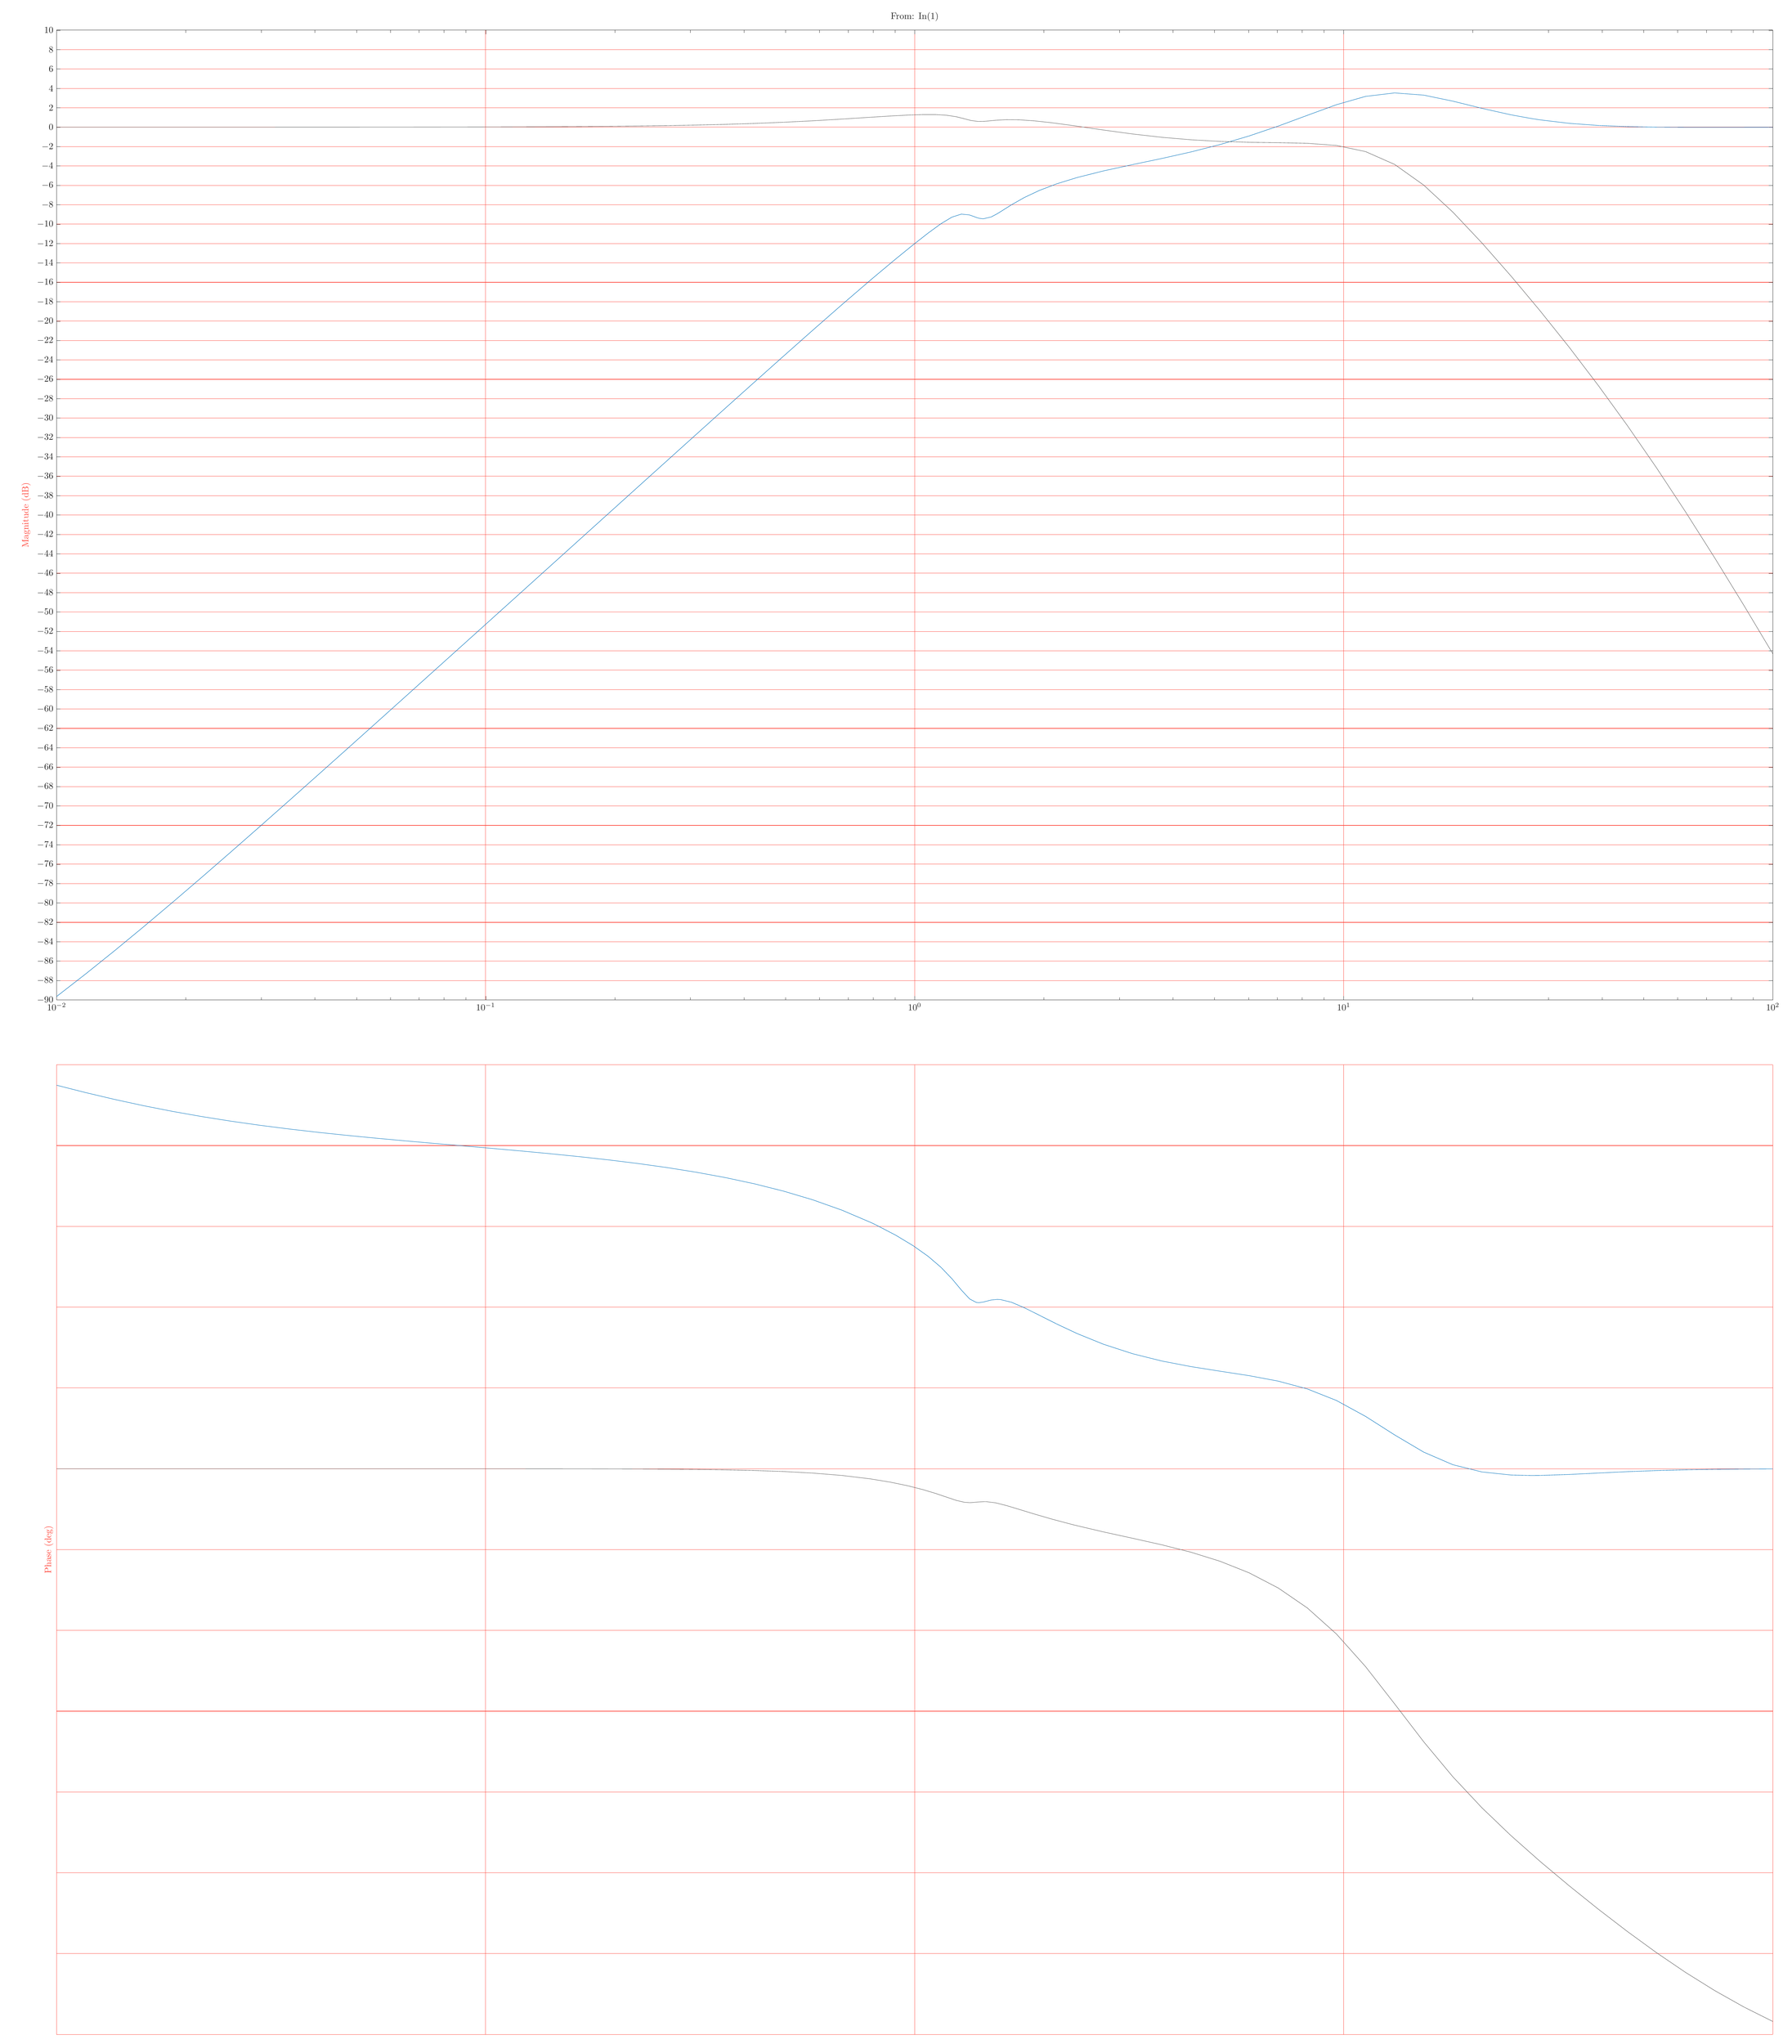
\begin{tikzpicture}

\begin{axis}[%
width=25.848in,
height=14.598in,
at={(0.714in,-15.264in)},
scale only axis,
unbounded coords=jump,
separate axis lines,
every outer x axis line/.append style={mycolor4},
every x tick label/.append style={font=\color{mycolor4}},
every x tick/.append style={mycolor4},
xmode=log,
xmin=0.01,
xmax=100,
xtick={0.01,0.1,1,10,100},
xticklabels={\empty},
xminorticks=true,
every outer y axis line/.append style={mycolor4},
every y tick label/.append style={font=\color{mycolor4}},
every y tick/.append style={mycolor4},
ymin=-315,
ymax=225,
ytick={-315,-270,-225,-180,-135,-90,-45,0,45,90,135,180,225},
yticklabels={\empty},
ylabel style={font=\color{mycolor5}},
ylabel={Phase (deg)},
axis line style={draw=none},
ticks=none,
xmajorgrids,
ymajorgrids,
grid style={mycolor5}
]
\addplot [color=mycolor1, line width=1.5pt, forget plot]
  table[row sep=crcr]{%
nan	-315\\
nan	225\\
};
\addplot [color=mycolor1, line width=1.5pt, forget plot]
  table[row sep=crcr]{%
nan	-315\\
nan	225\\
};
\addplot [color=mycolor1, line width=1.5pt, forget plot]
  table[row sep=crcr]{%
nan	-315\\
nan	225\\
};
\addplot [color=mycolor1, line width=1.5pt, forget plot]
  table[row sep=crcr]{%
nan	-315\\
nan	225\\
};
\addplot [color=mycolor2, forget plot]
  table[row sep=crcr]{%
-100	-0.0874059251163381\\
-85.5467253556568	-0.171290363079045\\
-73.1824221907617	-0.32414079596629\\
-62.6051657201482	-0.586763841646358\\
-53.556669177069	-1.00519159192558\\
-45.8159766905449	-1.61007048919653\\
-39.1940677484722	-2.37764941489578\\
-33.5292414924956	-3.17619336460478\\
-28.6831681334201	-3.71050637986811\\
-27.3649810756655	-3.75021130046122\\
-24.5375110663982	-3.47980969229867\\
-20.9910372010855	-1.76798774009749\\
-17.9571449437164	2.27304931725333\\
-15.3617494667183	9.2709323230947\\
-13.1414736261176	18.8581986691658\\
-11.2421003506209	29.1780579002396\\
-9.61724871115296	38.0241893751165\\
-8.22724134170047	44.4575318694928\\
-7.03813555493155	48.8037083334498\\
-6.02089449333613	51.842120876926\\
-5.15067807616812	54.3309918592856\\
-4.40623642777357	56.8875087817791\\
-3.76939097538836	59.9966302373703\\
-3.22459054529639	64.0384419382183\\
-2.75853161762918	69.2954432537248\\
-2.39237635077625	75.2779338137055\\
-2.14399148550878	80.6119470719379\\
-1.95196026166226	85.518310236875\\
-1.80130128659818	89.6759327575804\\
-1.68160667044661	92.7206378914625\\
-1.58548448116874	94.2249292995786\\
-1.55737457536084	94.3272319200869\\
-1.50757886072228	93.9797350047384\\
-1.44393831174424	92.8241983544655\\
-1.41074368011304	92.5001836207707\\
-1.39159923312488	92.6497986535288\\
-1.34516586651989	94.4842843459092\\
-1.34115731252706	94.7419909638751\\
-1.28454204027905	99.549454624222\\
-1.22142376581715	105.815566346838\\
-1.15160605608174	112.197104136092\\
-1.07508301917166	118.295849458072\\
-0.992104431462467	124.207178296335\\
-0.90324445722983	130.080257847349\\
-0.80946646417292	135.984626401748\\
-0.791234261898132	137.107805661084\\
-0.676875000945854	144.011501453475\\
-0.579044398060249	149.756692165831\\
-0.495353520895917	154.578959710467\\
-0.423758716060406	158.65670677078\\
-0.362511704998853	162.131003130561\\
-0.310116892657478	165.115002898965\\
-0.26529484644319	167.700544418529\\
-0.226951053669467	169.96324877457\\
-0.194149194574388	171.966459568183\\
-0.166088278262772	173.764261589217\\
-0.142083083253392	175.403797802981\\
-0.121547425007629	176.927071152147\\
-0.103979841848149	178.372375791458\\
-0.0889513497310823	179.775462349699\\
-0.0760949668545988	181.170507720051\\
-0.0650967523045817	182.590931243523\\
-0.0556881399094527	184.070073466094\\
-0.0476393801040134	185.641727688692\\
-0.0407539296587178	187.34048494213\\
-0.0348636522767809	189.201816897049\\
-0.0298247128621689	191.261777241919\\
-0.0255140652003129	193.556153001934\\
-0.0218264472839749	196.118854627315\\
-0.0186718109129192	198.979324538709\\
-0.0159731228006025	202.158817301028\\
-0.0136644834929533	205.665628883818\\
-0.0116895181649858	209.489784571786\\
-0.01	213.598305583323\\
0.01	213.598305583323\\
0.0116895181649858	209.489784571786\\
0.0136644834929533	205.665628883818\\
0.0159731228006025	202.158817301028\\
0.0186718109129192	198.979324538709\\
0.0218264472839749	196.118854627315\\
0.0255140652003129	193.556153001934\\
0.0298247128621689	191.261777241919\\
0.0348636522767809	189.201816897049\\
0.0407539296587178	187.34048494213\\
0.0476393801040134	185.641727688692\\
0.0556881399094527	184.070073466094\\
0.0650967523045817	182.590931243523\\
0.0760949668545988	181.170507720051\\
0.0889513497310823	179.775462349699\\
0.103979841848149	178.372375791458\\
0.121547425007629	176.927071152147\\
0.142083083253392	175.403797802981\\
0.166088278262772	173.764261589217\\
0.194149194574388	171.966459568183\\
0.226951053669467	169.96324877457\\
0.26529484644319	167.700544418529\\
0.310116892657478	165.115002898965\\
0.362511704998853	162.131003130561\\
0.423758716060406	158.65670677078\\
0.495353520895917	154.578959710467\\
0.579044398060249	149.756692165831\\
0.676875000945854	144.011501453475\\
0.791234261898132	137.107805661084\\
0.80946646417292	135.984626401748\\
0.90324445722983	130.080257847349\\
0.992104431462467	124.207178296335\\
1.07508301917166	118.295849458072\\
1.15160605608174	112.197104136092\\
1.22142376581715	105.815566346838\\
1.28454204027905	99.549454624222\\
1.34115731252706	94.7419909638751\\
1.34516586651989	94.4842843459092\\
1.39159923312488	92.6497986535288\\
1.41074368011304	92.5001836207707\\
1.44393831174424	92.8241983544655\\
1.50757886072228	93.9797350047384\\
1.55737457536084	94.3272319200869\\
1.58548448116874	94.2249292995786\\
1.68160667044661	92.7206378914625\\
1.80130128659818	89.6759327575804\\
1.95196026166226	85.518310236875\\
2.14399148550878	80.6119470719379\\
2.39237635077625	75.2779338137055\\
2.75853161762918	69.2954432537248\\
3.22459054529639	64.0384419382183\\
3.76939097538836	59.9966302373703\\
4.40623642777357	56.8875087817791\\
5.15067807616812	54.3309918592856\\
6.02089449333613	51.842120876926\\
7.03813555493155	48.8037083334498\\
8.22724134170047	44.4575318694928\\
9.61724871115296	38.0241893751165\\
11.2421003506209	29.1780579002396\\
13.1414736261176	18.8581986691658\\
15.3617494667183	9.2709323230947\\
17.9571449437164	2.27304931725333\\
20.9910372010855	-1.76798774009749\\
24.5375110663982	-3.47980969229867\\
27.3649810756655	-3.75021130046122\\
28.6831681334201	-3.71050637986811\\
33.5292414924956	-3.17619336460478\\
39.1940677484722	-2.37764941489578\\
45.8159766905449	-1.61007048919653\\
53.556669177069	-1.00519159192558\\
62.6051657201482	-0.586763841646358\\
73.1824221907617	-0.32414079596629\\
85.5467253556568	-0.171290363079045\\
100	-0.0874059251163381\\
};
\addplot [color=mycolor3, forget plot]
  table[row sep=crcr]{%
-100	-307.793018440645\\
-85.5467253556568	-299.664863494399\\
-73.1824221907617	-290.546391482923\\
-62.6051657201482	-280.452230704627\\
-53.556669177069	-269.451517136699\\
-45.8159766905449	-257.661345164767\\
-39.1940677484722	-245.216066688536\\
-33.5292414924956	-232.211520958182\\
-28.6831681334201	-218.634089794653\\
-24.5375110663982	-204.291318257886\\
-20.9910372010855	-188.769515143521\\
-17.9571449437164	-171.488215025333\\
-15.3617494667183	-152.035286873364\\
-13.1414736261176	-130.938987532268\\
-11.2421003506209	-110.172124838927\\
-9.61724871115296	-92.0287925883944\\
-8.22724134170047	-77.5237798019651\\
-7.03813555493155	-66.4052881547796\\
-6.02089449333613	-57.9668530620365\\
-5.15067807616812	-51.5143288413504\\
-4.40623642777357	-46.4715991887476\\
-3.76939097538836	-42.3553984521096\\
-3.22459054529639	-38.7323740277567\\
-2.75853161762918	-35.1966208710885\\
-2.35983346678219	-31.3844223477595\\
-2.33322936942428	-31.0887804557268\\
-2.09040651483373	-28.0611699795067\\
-1.90269341820247	-25.2311329820763\\
-1.75543293678617	-22.6764226581004\\
-1.63844422720746	-20.5187947097441\\
-1.54449782359004	-18.9717570593854\\
-1.46835641873509	-18.3141033721481\\
-1.45553358577972	-18.2984082256981\\
-1.40615656185632	-18.5040827448892\\
-1.35500109262074	-18.8403693675378\\
-1.34516586651989	-18.8606324341236\\
-1.34224796314547	-18.8618089966951\\
-1.30570664093022	-18.6574536111163\\
-1.250396659542	-17.6087930734653\\
-1.18875399690479	-15.8565420730849\\
-1.12059228536128	-13.7816282961633\\
-1.04591176485773	-11.6257107820322\\
-0.964962585899914	-9.49884194573737\\
-0.878311442283961	-7.46740913823664\\
-0.786904187416619	-5.59695019017315\\
-0.676875000945854	-3.72197362567678\\
-0.579044398060249	-2.40474987259807\\
-0.495353520895917	-1.53497880201413\\
-0.423758716060406	-0.969473854290734\\
-0.362511704998853	-0.606240951646049\\
-0.310116892657478	-0.375190510142921\\
-0.26529484644319	-0.229420176303192\\
-0.226951053669467	-0.138139077759752\\
-0.194149194574388	-0.0814105678620066\\
-0.166088278262772	-0.0464555453089879\\
-0.142083083253392	-0.0251443177270267\\
-0.121547425007629	-0.0123351170819639\\
-0.103979841848149	-0.00479142979390124\\
-0.0889513497310823	-0.000484595732336961\\
-0.0760949668545988	0.00185173421257914\\
-0.0650967523045817	0.00300453682554074\\
-0.0556881399094527	0.0034602956391395\\
-0.0500538326402051	0.00352981509900201\\
-0.0476393801040134	0.00351770493471817\\
-0.0407539296587178	0.00335848374944955\\
-0.0348636522767809	0.00309176329229372\\
-0.0298247128621689	0.00278184661088853\\
-0.0255140652003129	0.00246552797861774\\
-0.0218264472839749	0.00216286883757939\\
-0.0186718109129192	0.0018838795823746\\
-0.0159731228006025	0.0016326441671314\\
-0.0136644834929533	0.00140985071612701\\
-0.0116895181649858	0.00121433096586509\\
-0.01	0.00104398534524406\\
0.01	0.00104398534524406\\
0.0116895181649858	0.00121433096586509\\
0.0136644834929533	0.00140985071612701\\
0.0159731228006025	0.0016326441671314\\
0.0186718109129192	0.0018838795823746\\
0.0218264472839749	0.00216286883757939\\
0.0255140652003129	0.00246552797861774\\
0.0298247128621689	0.00278184661088853\\
0.0348636522767809	0.00309176329229372\\
0.0407539296587178	0.00335848374944955\\
0.0476393801040134	0.00351770493471817\\
0.0500538326402051	0.00352981509900201\\
0.0556881399094527	0.0034602956391395\\
0.0650967523045817	0.00300453682554074\\
0.0760949668545988	0.00185173421257914\\
0.0889513497310823	-0.000484595732336961\\
0.103979841848149	-0.00479142979390124\\
0.121547425007629	-0.0123351170819639\\
0.142083083253392	-0.0251443177270267\\
0.166088278262772	-0.0464555453089879\\
0.194149194574388	-0.0814105678620066\\
0.226951053669467	-0.138139077759752\\
0.26529484644319	-0.229420176303192\\
0.310116892657478	-0.375190510142921\\
0.362511704998853	-0.606240951646049\\
0.423758716060406	-0.969473854290734\\
0.495353520895917	-1.53497880201413\\
0.579044398060249	-2.40474987259807\\
0.676875000945854	-3.72197362567678\\
0.786904187416619	-5.59695019017315\\
0.878311442283961	-7.46740913823664\\
0.964962585899914	-9.49884194573737\\
1.04591176485773	-11.6257107820322\\
1.12059228536128	-13.7816282961633\\
1.18875399690479	-15.8565420730849\\
1.250396659542	-17.6087930734653\\
1.30570664093022	-18.6574536111163\\
1.34224796314547	-18.8618089966951\\
1.34516586651989	-18.8606324341236\\
1.35500109262074	-18.8403693675378\\
1.40615656185632	-18.5040827448892\\
1.45553358577972	-18.2984082256981\\
1.46835641873509	-18.3141033721481\\
1.54449782359004	-18.9717570593854\\
1.63844422720746	-20.5187947097441\\
1.75543293678617	-22.6764226581004\\
1.90269341820247	-25.2311329820763\\
2.09040651483373	-28.0611699795067\\
2.33322936942428	-31.0887804557268\\
2.35983346678219	-31.3844223477595\\
2.75853161762918	-35.1966208710885\\
3.22459054529639	-38.7323740277567\\
3.76939097538836	-42.3553984521096\\
4.40623642777357	-46.4715991887476\\
5.15067807616812	-51.5143288413504\\
6.02089449333613	-57.9668530620365\\
7.03813555493155	-66.4052881547796\\
8.22724134170047	-77.5237798019651\\
9.61724871115296	-92.0287925883944\\
11.2421003506209	-110.172124838927\\
13.1414736261176	-130.938987532268\\
15.3617494667183	-152.035286873364\\
17.9571449437164	-171.488215025333\\
20.9910372010855	-188.769515143521\\
24.5375110663982	-204.291318257886\\
28.6831681334201	-218.634089794653\\
33.5292414924956	-232.211520958182\\
39.1940677484722	-245.216066688536\\
45.8159766905449	-257.661345164767\\
53.556669177069	-269.451517136699\\
62.6051657201482	-280.452230704627\\
73.1824221907617	-290.546391482923\\
85.5467253556568	-299.664863494399\\
100	-307.793018440645\\
};
\end{axis}

\begin{axis}[%
width=25.848in,
height=14.598in,
at={(0.714in,0.309in)},
scale only axis,
unbounded coords=jump,
separate axis lines,
every outer x axis line/.append style={mycolor4},
every x tick label/.append style={font=\color{mycolor4}},
every x tick/.append style={mycolor4},
xmode=log,
xmin=0.01,
xmax=100,
xminorticks=true,
every outer y axis line/.append style={mycolor4},
every y tick label/.append style={font=\color{mycolor4}},
every y tick/.append style={mycolor4},
ymin=-90,
ymax=10,
ylabel style={font=\color{mycolor5}},
ylabel={Magnitude (dB)},
axis background/.style={fill=white},
title style={font=\color{mycolor4}},
title={From: In(1)},
xmajorgrids,
ymajorgrids,
grid style={mycolor5},
legend style={legend cell align=left, align=left}
]
\addplot [color=mycolor1, line width=1.5pt, forget plot]
  table[row sep=crcr]{%
nan	-90\\
nan	10\\
};
\addplot [color=mycolor1, line width=1.5pt, forget plot]
  table[row sep=crcr]{%
nan	-90\\
nan	10\\
};
\addplot [color=mycolor1, line width=1.5pt, forget plot]
  table[row sep=crcr]{%
nan	-90\\
nan	10\\
};
\addplot [color=mycolor1, line width=1.5pt, forget plot]
  table[row sep=crcr]{%
nan	-90\\
nan	10\\
};
\addplot [color=mycolor2, forget plot]
  table[row sep=crcr]{%
-100	-0.0102593899175354\\
-85.5467253556568	-0.0147389641584169\\
-73.1824221907617	-0.0182593409084535\\
-62.6051657201482	-0.0159391618062785\\
-53.556669177069	0.0027958442399825\\
-45.8159766905449	0.0569999577022069\\
-39.1940677484722	0.175620058132517\\
-33.5292414924956	0.395350580605923\\
-28.6831681334201	0.753227394285776\\
-27.3649810756655	0.892420833617155\\
-24.5375110663982	1.27300914267232\\
-20.9910372010855	1.94334421909099\\
-17.9571449437164	2.68367900962647\\
-15.3617494667183	3.30528120581239\\
-13.1414736261176	3.53119193170973\\
-11.2421003506209	3.1727643035267\\
-9.61724871115296	2.31622024239838\\
-8.22724134170047	1.2222493309579\\
-7.03813555493155	0.111028915490177\\
-6.02089449333613	-0.904934247134155\\
-5.15067807616812	-1.79090757294401\\
-4.40623642777357	-2.55457400553005\\
-3.76939097538836	-3.22688955767302\\
-3.22459054529639	-3.85533232170271\\
-2.75853161762918	-4.50490269134811\\
-2.39237635077625	-5.19097595246304\\
-2.14399148550878	-5.83996621039048\\
-1.95196026166226	-6.528086397306\\
-1.80130128659818	-7.25457633637081\\
-1.68160667044661	-8.00284393621597\\
-1.58548448116874	-8.71699128050133\\
-1.55737457536084	-8.9289661346214\\
-1.50757886072228	-9.25988167249043\\
-1.44393831174424	-9.4516695818925\\
-1.41074368011304	-9.3881879113604\\
-1.39159923312488	-9.30602062671002\\
-1.34516586651989	-9.06690513152701\\
-1.34115731252706	-9.04942444615172\\
-1.28454204027905	-8.96632338133879\\
-1.22142376581715	-9.27535016594847\\
-1.15160605608174	-9.95561351830388\\
-1.07508301917166	-10.9191062682273\\
-0.992104431462467	-12.1278314525266\\
-0.90324445722983	-13.5929423026605\\
-0.80946646417292	-15.3520814568389\\
-0.791234261898132	-15.7228787922617\\
-0.676875000945854	-18.3016184332281\\
-0.579044398060249	-20.9296042595755\\
-0.495353520895917	-23.5888106224719\\
-0.423758716060406	-26.2673166848359\\
-0.362511704998853	-28.9576464141489\\
-0.310116892657478	-31.6552170992662\\
-0.26529484644319	-34.3572222620607\\
-0.226951053669467	-37.0619122337741\\
-0.194149194574388	-39.7681526859365\\
-0.166088278262772	-42.4751570830934\\
-0.142083083253392	-45.1823215502855\\
-0.121547425007629	-47.8891170869398\\
-0.103979841848149	-50.5950114661502\\
-0.0889513497310823	-53.2994035435354\\
-0.0760949668545988	-56.0015584673237\\
-0.0650967523045817	-58.7005352274413\\
-0.0556881399094527	-61.3950993100894\\
-0.0476393801040134	-64.0836137834564\\
-0.0407539296587178	-66.7639026745256\\
-0.0348636522767809	-69.43308188942\\
-0.0298247128621689	-72.087356433351\\
-0.0255140652003129	-74.7217901007025\\
-0.0218264472839749	-77.3300674275207\\
-0.0186718109129192	-79.9042896437204\\
-0.0159731228006025	-82.4348765998667\\
-0.0136644834929533	-84.9106791604154\\
-0.0116895181649858	-87.3194244381211\\
-0.01	-89.6485901974779\\
0.01	-89.6485901974779\\
0.0116895181649858	-87.3194244381211\\
0.0136644834929533	-84.9106791604154\\
0.0159731228006025	-82.4348765998667\\
0.0186718109129192	-79.9042896437204\\
0.0218264472839749	-77.3300674275207\\
0.0255140652003129	-74.7217901007025\\
0.0298247128621689	-72.087356433351\\
0.0348636522767809	-69.43308188942\\
0.0407539296587178	-66.7639026745256\\
0.0476393801040134	-64.0836137834564\\
0.0556881399094527	-61.3950993100894\\
0.0650967523045817	-58.7005352274413\\
0.0760949668545988	-56.0015584673237\\
0.0889513497310823	-53.2994035435354\\
0.103979841848149	-50.5950114661502\\
0.121547425007629	-47.8891170869398\\
0.142083083253392	-45.1823215502855\\
0.166088278262772	-42.4751570830934\\
0.194149194574388	-39.7681526859365\\
0.226951053669467	-37.0619122337741\\
0.26529484644319	-34.3572222620607\\
0.310116892657478	-31.6552170992662\\
0.362511704998853	-28.9576464141489\\
0.423758716060406	-26.2673166848359\\
0.495353520895917	-23.5888106224719\\
0.579044398060249	-20.9296042595755\\
0.676875000945854	-18.3016184332281\\
0.791234261898132	-15.7228787922617\\
0.80946646417292	-15.3520814568389\\
0.90324445722983	-13.5929423026605\\
0.992104431462467	-12.1278314525266\\
1.07508301917166	-10.9191062682273\\
1.15160605608174	-9.95561351830388\\
1.22142376581715	-9.27535016594847\\
1.28454204027905	-8.96632338133879\\
1.34115731252706	-9.04942444615172\\
1.34516586651989	-9.06690513152701\\
1.39159923312488	-9.30602062671002\\
1.41074368011304	-9.3881879113604\\
1.44393831174424	-9.4516695818925\\
1.50757886072228	-9.25988167249043\\
1.55737457536084	-8.9289661346214\\
1.58548448116874	-8.71699128050133\\
1.68160667044661	-8.00284393621597\\
1.80130128659818	-7.25457633637081\\
1.95196026166226	-6.528086397306\\
2.14399148550878	-5.83996621039048\\
2.39237635077625	-5.19097595246304\\
2.75853161762918	-4.50490269134811\\
3.22459054529639	-3.85533232170271\\
3.76939097538836	-3.22688955767302\\
4.40623642777357	-2.55457400553005\\
5.15067807616812	-1.79090757294401\\
6.02089449333613	-0.904934247134155\\
7.03813555493155	0.111028915490177\\
8.22724134170047	1.2222493309579\\
9.61724871115296	2.31622024239838\\
11.2421003506209	3.1727643035267\\
13.1414736261176	3.53119193170973\\
15.3617494667183	3.30528120581239\\
17.9571449437164	2.68367900962647\\
20.9910372010855	1.94334421909099\\
24.5375110663982	1.27300914267232\\
27.3649810756655	0.892420833617155\\
28.6831681334201	0.753227394285776\\
33.5292414924956	0.395350580605923\\
39.1940677484722	0.175620058132517\\
45.8159766905449	0.0569999577022069\\
53.556669177069	0.0027958442399825\\
62.6051657201482	-0.0159391618062785\\
73.1824221907617	-0.0182593409084535\\
85.5467253556568	-0.0147389641584169\\
100	-0.0102593899175354\\
};
\addplot [color=mycolor3, forget plot]
  table[row sep=crcr]{%
-100	-54.296964784359\\
-85.5467253556568	-49.2822936634345\\
-73.1824221907617	-44.3952042400652\\
-62.6051657201482	-39.6639382713927\\
-53.556669177069	-35.1147274440719\\
-45.8159766905449	-30.7667147702661\\
-39.1940677484722	-26.6270824200043\\
-33.5292414924956	-22.6890129935726\\
-28.6831681334201	-18.9351192368707\\
-24.5375110663982	-15.3484585135229\\
-20.9910372010855	-11.9340211570091\\
-17.9571449437164	-8.75486257735047\\
-15.3617494667183	-5.97475616371706\\
-13.1414736261176	-3.84228180530961\\
-11.2421003506209	-2.51746663149253\\
-9.61724871115296	-1.88680227585221\\
-8.22724134170047	-1.66349961313188\\
-7.03813555493155	-1.60102966393889\\
-6.02089449333613	-1.5583115688302\\
-5.15067807616812	-1.46813423693083\\
-4.40623642777357	-1.30100072617729\\
-3.76939097538836	-1.0462552763128\\
-3.22459054529639	-0.706383047451502\\
-2.75853161762918	-0.299047767602812\\
-2.35983346678219	0.136717244208039\\
-2.33322936942428	0.167849237541713\\
-2.09040651483373	0.452225486457196\\
-1.90269341820247	0.649704934185318\\
-1.75543293678617	0.756821139449281\\
-1.63844422720746	0.77444106474894\\
-1.54449782359004	0.712831583936254\\
-1.46835641873509	0.618247055670133\\
-1.45553358577972	0.60436144641712\\
-1.40615656185632	0.589353905328126\\
-1.35500109262074	0.683551000544188\\
-1.34516586651989	0.715229670275074\\
-1.34224796314547	0.725283000199988\\
-1.30570664093022	0.866872390990114\\
-1.250396659542	1.0749631536716\\
-1.18875399690479	1.22601954763167\\
-1.12059228536128	1.29685588997506\\
-1.04591176485773	1.29917662441158\\
-0.964962585899914	1.24747482897113\\
-0.878311442283961	1.15156402702689\\
-0.786904187416619	1.01934831250934\\
-0.676875000945854	0.833451520016346\\
-0.579044398060249	0.656975178499496\\
-0.495353520895917	0.507180034753395\\
-0.423758716060406	0.385785110009493\\
-0.362511704998853	0.290349348973241\\
-0.310116892657478	0.21685774232818\\
-0.26529484644319	0.161073973526351\\
-0.226951053669467	0.119160188820535\\
-0.194149194574388	0.0878957628441003\\
-0.166088278262772	0.0646963977874076\\
-0.142083083253392	0.0475464207841158\\
-0.121547425007629	0.0349030337510706\\
-0.103979841848149	0.0256005220880226\\
-0.0889513497310823	0.0187659937665499\\
-0.0760949668545988	0.0137499810241045\\
-0.0650967523045817	0.0100714513711788\\
-0.0556881399094527	0.00737529169158553\\
-0.0500538326402051	0.00596040012158581\\
-0.0476393801040134	0.00539996722673523\\
-0.0407539296587178	0.0039531929767675\\
-0.0348636522767809	0.00289377420298055\\
-0.0298247128621689	0.00211812605927781\\
-0.0255140652003129	0.00155030592414\\
-0.0218264472839749	0.00113466388849676\\
-0.0186718109129192	0.00083043475186569\\
-0.0159731228006025	0.000607764527202388\\
-0.0136644834929533	0.000444794080756826\\
-0.0116895181649858	0.000325520336096573\\
-0.01	0.000238228622922885\\
0.01	0.000238228622922885\\
0.0116895181649858	0.000325520336096573\\
0.0136644834929533	0.000444794080756826\\
0.0159731228006025	0.000607764527202388\\
0.0186718109129192	0.00083043475186569\\
0.0218264472839749	0.00113466388849676\\
0.0255140652003129	0.00155030592414\\
0.0298247128621689	0.00211812605927781\\
0.0348636522767809	0.00289377420298055\\
0.0407539296587178	0.0039531929767675\\
0.0476393801040134	0.00539996722673523\\
0.0500538326402051	0.00596040012158581\\
0.0556881399094527	0.00737529169158553\\
0.0650967523045817	0.0100714513711788\\
0.0760949668545988	0.0137499810241045\\
0.0889513497310823	0.0187659937665499\\
0.103979841848149	0.0256005220880226\\
0.121547425007629	0.0349030337510706\\
0.142083083253392	0.0475464207841158\\
0.166088278262772	0.0646963977874076\\
0.194149194574388	0.0878957628441003\\
0.226951053669467	0.119160188820535\\
0.26529484644319	0.161073973526351\\
0.310116892657478	0.21685774232818\\
0.362511704998853	0.290349348973241\\
0.423758716060406	0.385785110009493\\
0.495353520895917	0.507180034753395\\
0.579044398060249	0.656975178499496\\
0.676875000945854	0.833451520016346\\
0.786904187416619	1.01934831250934\\
0.878311442283961	1.15156402702689\\
0.964962585899914	1.24747482897113\\
1.04591176485773	1.29917662441158\\
1.12059228536128	1.29685588997506\\
1.18875399690479	1.22601954763167\\
1.250396659542	1.0749631536716\\
1.30570664093022	0.866872390990114\\
1.34224796314547	0.725283000199988\\
1.34516586651989	0.715229670275074\\
1.35500109262074	0.683551000544188\\
1.40615656185632	0.589353905328126\\
1.45553358577972	0.60436144641712\\
1.46835641873509	0.618247055670133\\
1.54449782359004	0.712831583936254\\
1.63844422720746	0.77444106474894\\
1.75543293678617	0.756821139449281\\
1.90269341820247	0.649704934185318\\
2.09040651483373	0.452225486457196\\
2.33322936942428	0.167849237541713\\
2.35983346678219	0.136717244208039\\
2.75853161762918	-0.299047767602812\\
3.22459054529639	-0.706383047451502\\
3.76939097538836	-1.0462552763128\\
4.40623642777357	-1.30100072617729\\
5.15067807616812	-1.46813423693083\\
6.02089449333613	-1.5583115688302\\
7.03813555493155	-1.60102966393889\\
8.22724134170047	-1.66349961313188\\
9.61724871115296	-1.88680227585221\\
11.2421003506209	-2.51746663149253\\
13.1414736261176	-3.84228180530961\\
15.3617494667183	-5.97475616371706\\
17.9571449437164	-8.75486257735047\\
20.9910372010855	-11.9340211570091\\
24.5375110663982	-15.3484585135229\\
28.6831681334201	-18.9351192368707\\
33.5292414924956	-22.6890129935726\\
39.1940677484722	-26.6270824200043\\
45.8159766905449	-30.7667147702661\\
53.556669177069	-35.1147274440719\\
62.6051657201482	-39.6639382713927\\
73.1824221907617	-44.3952042400652\\
85.5467253556568	-49.2822936634345\\
100	-54.296964784359\\
};
\end{axis}

\begin{axis}[%
width=26.667in,
height=15in,
at={(0in,0in)},
scale only axis,
xmin=0,
xmax=1,
ymin=0,
ymax=1,
axis line style={draw=none},
ticks=none,
axis x line*=bottom,
axis y line*=left
]
\end{axis}
\end{tikzpicture}%}
\caption{Sensitivity functions for Design C: $S(s)$ (blue) shows disturbance rejection capability, while $T(s)$ (red) indicates tracking bandwidth and noise attenuation characteristics.}
\label{fig:sensitivity_functions}
\end{figure}

\paragraph{Room for Improvement.}

The final design achieves all primary specifications, but several enhancements could be considered. First, a \textbf{notch filter for Dutch roll} could address the lightly-damped plant mode at 1.37~rad/s ($\zeta=0.13$) that persists in closed loop. Adding a notch filter $C_{\text{notch}}(s) = \frac{s^2 + 2(0.13)(1.37)s + 1.37^2}{s^2 + 2(0.70)(1.37)s + 1.37^2}$ would improve passenger comfort by damping residual Dutch roll oscillations, though at the cost of increased controller complexity. Second, a \textbf{reference pre-filter} $F(s) = 1/(1+s/\omega_r)$ with $\omega_r \approx 4$~rad/s could smooth aggressive commands, reducing the 10.8\% overshoot caused by actuator saturation without changing loop dynamics. Third, \textbf{gain scheduling} could maintain performance across the flight envelope, as controller parameters were optimized for 120~knots at 400~ft; scheduling $K$, $z_\ell$, $p_\ell$ as functions of dynamic pressure $\bar{q}$ or airspeed $V$ would extend operating range. Fourth, \textbf{actuator rate limiting} considerations are warranted, as the current design assumes instantaneous actuator response limited only by position; adding rate constraints ($\dot{\delta}_a < 50^\circ$/s typical) would require model predictive control or adaptive anti-windup to prevent performance degradation.

However, for the specified requirements and operating point, \textbf{Design C represents an excellent balance between performance, robustness, and implementation simplicity}. The 73$^\circ$ phase margin provides substantial robustness to modeling uncertainties and parameter variations.

\paragraph{Final Compensator Transfer Function.}

\begin{equation}
\boxed{~
C_{\mathrm{WL}}(s) = -0.1643 \cdot
\frac{1 + s/2.227}{1 + s/28.0} \cdot
\left(1 + \frac{1}{0.694\,s}\right) \cdot
\frac{1}{1 + s/28}
~}
\label{eq:final_controller}
\end{equation}

Expanded form:
\begin{equation}
C_{\mathrm{WL}}(s) = \frac{-0.1643(1 + 0.449s)(1 + 1.443/s)}{(1 + 0.0357s)(1 + 0.0357s)}
= \frac{-0.237s^2 - 0.386s - 0.237}{0.00128s^3 + 0.0714s^2 + s}
\end{equation}

This controller is implemented in MATLAB/Simulink with anti-windup logic for the integrator state when $|\delta_a| = 20^\circ$.

\subsection{Heading Hold Guidance Loop (HHGL) Compensator Design and Analysis}

Design a heading hold guidance loop that incorporates the wing-levelling autopilot as an inner loop. The guidance loop should use a compensator in the forward leg of the loop to convert heading (Yaw angle) error ($\Delta \psi$) into a bank angle command ($\phi_c$).

\textit{[Content to be continued for HHGL design...]}

\subsubsection{HHGL Loop Architecture}

\subsubsection{HHGL Plant Transfer Function}

\subsubsection{HHGL Compensator Design Strategy and Final Compensator}

\subsubsection{HHGL Frequency Response}

\subsubsection{HHGL Primary Control Effect}

\subsubsection{HHGL Inner Loop Response}

\subsubsection{HHGL Actuator Activity}

\subsection{HHGL Gust Response}

\textit{[Content for gust response analysis...]}

\subsubsection{HHGL Gust Transfer Functions}

\subsubsection{Lateral Open-Loop Gust Spectra and Excursion Analysis}

\subsubsection{HHG Gust Spectra and Excursion Analysis}

\subsection{Yaw Damper (YD) Compensator Design and Analysis}

\textit{[Content for yaw damper design...]}

\subsubsection{Lateral MIMO Loop Architecture}

\subsubsection{MIMO Loop Plant Transfer Functions}

\subsubsection{YD Compensator Design Strategy and Final Compensator}

\subsubsection{Re-evaluation of WL and HHGL Performance with YD}

\subsubsection{WL Compensator Re-Design}

\subsubsection{HHGL Compensator Re-Design}

\subsection{Lateral MIMO System Response}

\textit{[Content for MIMO system analysis...]}

\subsubsection{Primary Control Effects Analysis}

\subsubsection{Yaw Damper Effects Analysis}
